% ======================================================================
% guide.tex
% Copyright (c) Markus Kohm, 2002-2015
%
% This file is part of the LaTeX2e KOMA-Script bundle.
%
% This work may be distributed and/or modified under the conditions of
% the LaTeX Project Public License, version 1.3c of the license.
% The latest version of this license is in
%   http://www.latex-project.org/lppl.txt
% and version 1.3c or later is part of all distributions of LaTeX 
% version 2005/12/01 or later and of this work.
%
% This work has the LPPL maintenance status "author-maintained".
%
% The Current Maintainer and author of this work is Markus Kohm.
%
% This work consists of all files listed in manifest.txt.
% ----------------------------------------------------------------------
% guide.tex
% Copyright (c) Markus Kohm, 2002-2015
%
% Dieses Werk darf nach den Bedingungen der LaTeX Project Public Lizenz,
% Version 1.3c, verteilt und/oder veraendert werden.
% Die neuste Version dieser Lizenz ist
%   http://www.latex-project.org/lppl.txt
% und Version 1.3c ist Teil aller Verteilungen von LaTeX
% Version 2005/12/01 oder spaeter und dieses Werks.
%
% Dieses Werk hat den LPPL-Verwaltungs-Status "author-maintained"
% (allein durch den Autor verwaltet).
%
% Der Aktuelle Verwalter und Autor dieses Werkes ist Markus Kohm.
% 
% Dieses Werk besteht aus den in manifest.txt aufgefuehrten Dateien.
% ======================================================================
%
% Main TeX file of the KOMA-Script guide
% Maintained by Markus Kohm
%
% ----------------------------------------------------------------------
%
% Hauptdatei der KOMA-Script-Anleitung
% Verwaltet von Markus Kohm
%
% ======================================================================

\documentclass[\languagename]{scrguide}

\KOMAProvidesFile{guide.tex}
                 [$Date: 2015-04-21 10:08:26 +0200 (Tue, 21 Apr 2015) $
                  KOMA-Script (guide main file)]

\begin{document}
\expandafter\selectlanguage\expandafter{\uselanguage}

\csname ListTypeArea\endcsname

\extratitle{\sffamily{\bfseries\Huge\GuideTitle\strut\\}
  \large\GuideSubTitle\strut\\}
\title{\GuideTitle}
\subject{\GuideSubject}
\author{Markus Kohm}
\publishers{\small\GuideAuthorHeadline:
  Frank Neukam, Markus Kohm, Axel Kielhorn}
\uppertitleback{%
  \GuideWarrantyHeadline\\[.5\baselineskip]
  \GuideWarranty}
\lowertitleback{%
  \settranslator{\GuideTranslatorHeadline}{.\par\bigskip}%
  \GuideCopyright}
\dedication{\GuideDedication}

\pdfbookmark[-1]{\KOMAScript}{title}
\bookmark[level=0,gotor=scrguide.pdf]{Deutsch}
\bookmark[level=0,gotor=scrguien.pdf]{English}
\bookmarksetup{startatroot}

\maketitle

\cleardoublepage\csname GeneralTypeArea\endcsname
% ======================================================================
% preface.tex
% Copyright (c) Markus Kohm, 2008-2017
%
% This file is part of the LaTeX2e KOMA-Script bundle.
%
% This work may be distributed and/or modified under the conditions of
% the LaTeX Project Public License, version 1.3c of the license.
% The latest version of this license is in
%   http://www.latex-project.org/lppl.txt
% and version 1.3c or later is part of all distributions of LaTeX
% version 2005/12/01 or later and of this work.
%
% This work has the LPPL maintenance status "author-maintained".
%
% The Current Maintainer and author of this work is Markus Kohm.
%
% This work consists of all files listed in manifest.txt.
% ----------------------------------------------------------------------
% preface.tex
% Copyright (c) Markus Kohm, 2008-2017
%
% Dieses Werk darf nach den Bedingungen der LaTeX Project Public Lizenz,
% Version 1.3c, verteilt und/oder veraendert werden.
% Die neuste Version dieser Lizenz ist
%   http://www.latex-project.org/lppl.txt
% und Version 1.3c ist Teil aller Verteilungen von LaTeX
% Version 2005/12/01 oder spaeter und dieses Werks.
%
% Dieses Werk hat den LPPL-Verwaltungs-Status "author-maintained"
% (allein durch den Autor verwaltet).
%
% Der Aktuelle Verwalter und Autor dieses Werkes ist Markus Kohm.
%
% Dieses Werk besteht aus den in manifest.txt aufgefuehrten Dateien.
% ======================================================================

\KOMAProvidesFile{typearea.tex}
                 [$Date: 2017-01-16 09:00:06 +0100 (Mon, 16 Jan 2017) $
                  Vorwort nach Version 3.22]

\addchap{Vorwort zu \KOMAScript~3.22a}

Nachdem mit \KOMAScript~3 auch eine strukturell und inhaltlich komplett
�berarbeitete Anleitung erschienen ist, haben mich in den letzten Jahren nur
noch wenige Kritiken daran erreicht. Offenbar hat es sich auch gelohnt, das
Kapitel �ber Briefe um unz�hlige Beispiele zu erweitern und inhaltlich von dem
der anderen Klassen weitgehend unabh�ngig zu machen. Obwohl dadurch diverse
Abschnitte, wenn auch oftmals mit abgewandelten oder mit ausgelassenen
Beispielen, mehrfach \iffree{in der Anleitung}{im Buch} enthalten sind, wurde
dieses Vorgehen daher ab \iffree{\KOMAScript~3.22}{der sechsten Auflage} noch
konsequenter angewandt und auch auf andere Kapitel �bertragen.

\iffree{Die freie \KOMAScript-Anleitung wurde dar�ber hinaus farblich neu
  gestaltet und mit unz�hligen, neuen Links versehen. Au�er in ihrer
  unmittelbaren Beschreibung f�hrt ein Klick beispielsweise auf ein
  \KOMAScript-Makro nun daher auf die jeweils passende Erkl�rung. Querverweise
  mit der Nummer des passenden Abschnitts oder der Seitenzahl sind dennoch
  weiterhin vorhanden. Dies ist dem gedruckten Buch geschuldet und dient
  dar�ber hinaus der Orientierung.}{}

\iffree{Leser dieser freien Bildschirm-Version m�ssen allerdings weiterhin mit
  einigen Einschr�nkungen leben. So sind einige Informationen --
  haupts�chliche solche f�r fortgeschrittene Anwender oder die dazu geeignet
  sind, aus einem Anwender einen fortgeschrittenen Anwender zu machen -- der
  Buchfassung vorbehalten. Das f�hrt auch dazu, dass weiterhin einige Links in
  dieser Anleitung lediglich zu einer Seite f�hren, auf der genau diese
  Tatsache erw�hnt ist. Dar�ber hinaus ist die freie Version nur eingeschr�nkt
  zum Ausdruck geeignet. Der Fokus liegt vielmehr auf der Verwendung am
  Bildschirm parallel zur Arbeit an einem Dokument. Sie hat auch weiterhin
  keinen optimierten Umbruch, sondern ist quasi ein erster Entwurf, bei dem
  sowohl der Absatz- als auch der Seitenumbruch in einigen F�llen durchaus
  d�rftig ist. Entsprechende Optimierungen sind der Buchausgabe
  \cite{book:komascript} vorbehalten.}{}

Nicht nur zur Anleitung erfahre ich inzwischen eher wenig Kritik. Auch zu den
Klassen und Paketen gibt es kaum noch Nachfragen nach neuen M�glichkeiten. F�r
mich selbst bedeutet das, dass das Wissen um die W�nsche der Anwender
stagniert. Schon seit einigen Jahren habe ich daher haupts�chlich Dinge
implementiert, von denen ich annahm, dass sie n�tzlich sein k�nnten. Die
R�ckmeldungen, die ich zu diesen neuen M�glichkeiten erhalten habe,
beschr�nken sich aber �berwiegend auf Kritik daran, dass uralte \emph{Hacks},
die sich auf undokumentierte Eigenschaften von \KOMAScript{} st�tzen, in
einigen F�llen nicht mehr funktionieren. Freude dar�ber, dass derart unsaubere
Notl�sungen nicht mehr notwendig sind, wurde hingegen kaum ge�u�ert. Daher
habe ich beschlossen, Erweiterungen und Verbesserungen an \KOMAScript{} mehr
und mehr auf solche Dinge zu beschr�nken, die von Anwendern explizit
nachgefragt werden. Oder sollte es gar sein, dass \KOMAScript{} nach bald
25~Jahren schlicht einen Stand erreicht hat, in dem es alle W�nsche erf�llt?

Die r�ckl�ufige Entwicklung bei Fehlermeldungen ist leider ebenfalls nicht nur
erfreulich. Inzwischen ist h�ufig zu beobachten, dass diejenigen, die ein
Problem entdecken, dieses nicht mehr unmittelbar an mich melden, sondern sich
lediglich in irgendwelchen Internet-Foren dar�ber auslassen. Oftmals finden
sich in diesen Foren dann mehr oder weniger geschickte Notl�sungen. Das ist
zwar grunds�tzlich erfreulich, f�hrt aber leider in der Regel dazu, dass das
Problem nie gemeldet und daher auch nie wirklich beseitigt wird. Dass solche
Notl�sungen irgendwann selbst zu einem Problem werden k�nnen, versteht sich
von selbst und wurde bereits im vorherigen Absatz erw�hnt.

Vereinzelt finden sich dankenswerter Weise Dritte, die mich auf solche Themen
hinweisen. Dies betrifft aber nur einzelne Beitr�ge in sehr wenigen Foren. Ein
direkter Kontakt zu demjenigen, bei dem das Problem aufgetreten ist, ist dann
meist nicht m�glich, obwohl er teilweise w�nschenswert w�re.

Daher sei noch einmal ausdr�cklich darum gebeten, mir vermeintliche Bugs
wahlweise in Deutsch oder Englisch unmittelbar zu melden. Dabei ist
sprachliche Perfektion weniger wichtig. Die Meldung sollte halbwegs
verst�ndlich und das Problem nachvollziehbar sein. Ein m�glichst kurzes
Code-Beispiel ist in der Regel unabh�ngig von der darin verwendeten Sprache zu
verstehen. Im direkten Kontakt sind mir bei Bedarf auch R�ckfragen
m�glich. Bitte verlassen Sie sich nicht darauf, dass irgendwer das Problem
schon irgendwann melden wird. Gehen Sie davon aus, dass es nur behoben wird,
wenn Sie es selbst melden. N�heres zu Fehlermeldungen ist im ersten Kapitel
\iffree{der Anleitung}{des Buches} zu finden.

\bigskip\noindent
Markus Kohm, Neckarhausen bei eisigen Temperaturen im Januar 2017
\endinput

%%% Local Variables: 
%%% mode: latex
%%% coding: iso-latin-1
%%% TeX-master: "../guide.tex"
%%% End: 



\cleardoublepage\csname ListTypeArea\endcsname
\cleardoublepage\pdfbookmark{\contentsname}{toc}\tableofcontents

\cleardoublepage\pdfbookmark{\listfigurename}{lof}\listoffigures

\cleardoublepage\pdfbookmark{\listtablename}{lot}\listoftables

\cleardoublepage\csname GeneralTypeArea\endcsname

% ======================================================================
% introduction.tex
% Copyright (c) Markus Kohm, 2001-2017
%
% This file is part of the LaTeX2e KOMA-Script bundle.
%
% This work may be distributed and/or modified under the conditions of
% the LaTeX Project Public License, version 1.3c of the license.
% The latest version of this license is in
%   http://www.latex-project.org/lppl.txt
% and version 1.3c or later is part of all distributions of LaTeX 
% version 2005/12/01 or later and of this work.
%
% This work has the LPPL maintenance status "author-maintained".
%
% The Current Maintainer and author of this work is Markus Kohm.
%
% This work consists of all files listed in manifest.txt.
% ----------------------------------------------------------------------
% introduction.tex
% Copyright (c) Markus Kohm, 2001-2017
%
% Dieses Werk darf nach den Bedingungen der LaTeX Project Public Lizenz,
% Version 1.3c, verteilt und/oder veraendert werden.
% Die neuste Version dieser Lizenz ist
%   http://www.latex-project.org/lppl.txt
% und Version 1.3c ist Teil aller Verteilungen von LaTeX
% Version 2005/12/01 oder spaeter und dieses Werks.
%
% Dieses Werk hat den LPPL-Verwaltungs-Status "author-maintained"
% (allein durch den Autor verwaltet).
%
% Der Aktuelle Verwalter und Autor dieses Werkes ist Markus Kohm.
% 
% Dieses Werk besteht aus den in manifest.txt aufgefuehrten Dateien.
% ======================================================================
%
% Introduction of the KOMA-Script guide
% Maintained by Markus Kohm
%
% ----------------------------------------------------------------------
%
% Einleitung der KOMA-Script-Anleitung
% Verwaltet von Markus Kohm
%
% ======================================================================

\KOMAProvidesFile{introduction.tex}
                 [$Date: 2017-01-02 13:30:07 +0100 (Mon, 02 Jan 2017) $
                  KOMA-Script guide introduction]

\chapter{Einleitung}
\labelbase{introduction}

Dieses Kapitel enth�lt \iffree{unter anderem }{}wichtige Informationen �ber
den Aufbau \iffree{der Anleitung}{des Buches} und die Geschichte von
\KOMAScript, die Jahre vor der ersten Version beginnt. Dar�ber hinaus finden
Sie Informationen f�r den Fall, dass Sie %
\iffalse % Umbruchkorreturauslassung
 \KOMAScript{} noch nicht installiert haben, oder %
\fi%
auf Fehler sto�en.

\iffree{%
\section{Vorwort}
\seclabel{preface}

{\KOMAScript} ist ein sehr komplexes Paket (engl. \emph{bundle}). Dies
ist schon allein darin begr�ndet, dass es nicht nur aus einer einzigen
Klasse (engl. \emph{class}) oder einem einzigen Paket (engl.
\emph{package}), sondern einer Vielzahl derer besteht. Zwar sind die
Klassen als Gegenst�cke zu den Standardklassen konzipiert (siehe
\autoref{cha:maincls}), das hei�t jedoch insbesondere nicht,
dass sie nur �ber die Befehle, Umgebungen und Einstellm�glichkeiten
der Standardklassen verf�gen oder deren Aussehen als
Standardeinstellung �bernehmen.
Die F�higkeiten von {\KOMAScript} reichen
teilweise weit �ber die F�higkeiten der Standardklassen hinaus.
Manche davon sind auch als Erg�nzung zu den Grundf�higkeiten des
\LaTeX-Kerns zu betrachten.

Allein aus dem Vorgenannten ergibt sich schon zwangsl�ufig, dass die
Dokumentation zu {\KOMAScript} sehr umfangreich ausf�llt. Hinzu kommt,
dass {\KOMAScript} in der Regel nicht gelehrt wird. Das hei�t, es gibt
keinen Lehrer, der seine Sch�ler kennt und damit den Unterricht und
das Unterrichtsmaterial entsprechend w�hlen und anpassen kann. Es w�re
ein Leichtes, die Dokumentation f�r irgendeine Zielgruppe zu
verfassen.  Die Schwierigkeit, der sich der Autor gegen�ber sieht,
besteht jedoch darin, dass eine Anleitung f�r alle m�glichen
Zielgruppen ben�tigt wird. Ich habe mich bem�ht, eine Anleitung zu
erstellen, die f�r den Informatiker gleicherma�en geeignet ist wie f�r
die Sekret�rin des Fischh�ndlers. Ich habe mich bem�ht, obwohl es sich
dabei eigentlich um ein unm�gliches Unterfangen handelt. Ergebnis sind
zahlreiche Kompromisse. Ich bitte jedoch, die Problematik bei
eventuellen Beschwerden zu ber�cksichtigen und bei der Verbesserung
der derzeitigen L�sung zu helfen.

Trotz des Umfangs der Anleitung bitte ich au�erdem darum, im Falle von
Problemen zun�chst die Dokumentation zu konsultieren. Als erste Anlaufstelle
sei auf den mehrteiligen Index am Ende des \iffree{Dokuments}{Buches}
hingewiesen. \iffree{Zur Dokumentation geh�ren neben dieser Anleitung auch
  alle Text-Dokumente, die Bestandteil des Pakets sind. Sie sind in
  \File{manifest.txt} vollst�ndig aufgef�hrt}{}
}{}

\section{Dokumentaufbau}
\seclabel{structure}

Diese Anleitung ist in mehrere Teile untergliedert. Es gibt einen Teil f�r
Anwender, einen f�r fortgeschrittene Anwender und Experten und einen Anhang
mit weiterf�hrenden Informationen und Beispielen f�r diejenigen, die es ganz
genau wissen wollen.

\autoref{part:forAuthors} richtet sich dabei an alle \KOMAScript-Anwender. Das
bedeutet, dass hier auch einige Informationen f�r \LaTeX-Neulinge zu finden
sind. Insbesondere ist dieser Teil mit vielen Beispielen angereichert, die dem
reinen Anwender zur Verdeutlichung der Erkl�rungen dienen sollen. Scheuen Sie
sich nicht, diese Beispiele selbst auszuprobieren und durch Abwandlung
herauszufinden, wie \KOMAScript{} funktioniert. Trotz allem ist diese
Anleitung jedoch keine Einf�hrung in \LaTeX. \LaTeX-Neulingen seien daher
Dokumente wie \cite{l2kurz} nahe gelegt. Wiedereinsteiger aus der Zeit von
\LaTeX~2.09 sei zumindest \cite{latex:usrguide} empfohlen. Auch das Studium des
einen oder anderen Buches zu \LaTeX{} wird empfohlen.  Literaturempfehlungen
finden sich beispielsweise in \cite{DANTE:FAQ}. Der Umfang von
\cite{DANTE:FAQ} ist ebenfalls erheblich. Dennoch wird darum gebeten, das
Dokument nicht nur irgendwo vorliegen zu haben, sondern es mindestens einmal
zu lesen und bei Problemen zu konsultieren.

\autoref{part:forExperts} richtet sich an fortgeschrittene
\KOMAScript-Anwender. Das sind all diejenigen, die sich bereits mit \LaTeX{}
auskennen oder schon einige Zeit mit \KOMAScript{} gearbeitet haben und jetzt
etwas besser verstehen wollen, wie \KOMAScript{} funktioniert, wie es mit
anderen Paketen interagiert und wie man speziellere Aufgaben mit \KOMAScript{}
l�sen kann. Dazu werden die Klassenbeschreibungen aus
\autoref{part:forAuthors} in einigen Aspekten nochmals aufgegriffen und n�her
erl�utert. Dazu kommt die Dokumentation von Anweisungen, die speziell f�r
fortgeschrittene Anwender und Experten vorgesehen sind. Erg�nzt wird dies
durch die Dokumentation von Paketen, die f�r den Anwender normalerweise insofern
verborgen sind, als sie unter der Oberfl�che der Klassen und Anwenderpakete
ihre Arbeit verrichten. Diese Pakete sind ausdr�cklich auch f�r die Verwendung
durch andere Klassen- und Paketautoren vorgesehen.

Der Anhang\iffree{, der nur in der Buchfassung zu finden ist,}{} richtet sich
an diejenigen, denen all diese Informationen nicht gen�gen. Es gibt dort zum
einen Hintergrundwissen zu Fragen der Typografie, mit denen dem
fortgeschrittenen Anwender eine Grundlage f�r fundierte eigene Entscheidungen
vermittelt werden soll. Dar�ber hinaus sind dort Beispiele f�r angehende
Paketautoren zu finden. Diese Beispiele sind weniger dazu gedacht, einfach
�bernommen zu werden. Vielmehr sollen sie Wissen um Planung und Durchf�hrung
von \LaTeX-Projekten sowie einiger grundlegender \LaTeX-Anweisungen f�r
Paketautoren vermitteln.

Die Kapitel-Einteilung der Anleitung soll ebenfalls dabei
helfen, nur die Teile lesen zu m�ssen, die tats�chlich von Interesse sind. Um
dies zu erreichen, sind die Informationen zu den einzelnen Klassen und Paketen
nicht �ber das gesamte Dokument verteilt, sondern jeweils in einem Kapitel
konzentriert. Querverweise in ein anderes Kapitel sind damit in der Regel auch
Verweise auf einen anderen Teil des Gesamtpakets. Da die drei Hauptklassen in
weiten Teilen �bereinstimmen, sind sie in einem gemeinsamen Kapitel
zusammengefasst. Die Unterschiede werden deutlich hervorgehoben, soweit
sinnvoll auch durch eine entsprechende Randnotiz. Dies geschieht
beispielsweise wie hier, wenn etwas nur die Klasse
\Class{scrartcl}\OnlyAt{\Class{scrartcl}} betrifft. Nachteil dieses Vorgehens
ist, dass diejenigen, die \KOMAScript{} insgesamt kennenlernen wollen, in
einigen Kapiteln auf bereits Bekanntes sto�en werden. Vielleicht nutzen Sie
die Gelegenheit, um Ihr Wissen zu vertiefen.

Unterschiedliche Schriftarten werden auch zur Hervorhebung unterschiedlicher
Dinge verwendet. So werden die Namen von \Package{Paketen} und \Class{Klassen}
anders angezeigt als \File{Dateinamen}. \Option{Optionen}, \Macro{Anweisungen},
\Environment{Umgebungen}, \Variable{Variablen} und
\PLength{Pseudol�ngen} werden einheitlich hervorgehoben. Der
\PName{Platzhalter} f�r einen Parameter wird jedoch anders dargestellt als ein
konkreter \PValue{Wert} eines Parameters. So zeigt etwa
\Macro{begin}\Parameter{Umgebung}, wie eine Umgebung ganz allgemein
eingeleitet wird, wohingegen \Macro{begin}\PParameter{document} angibt, wie die
konkrete Umgebung \Environment{document} beginnt. Dabei ist dann
\PValue{document} ein konkreter Wert f�r den Parameter \PName{Umgebung}
der Anweisung \Macro{begin}.

\iffalse% Umbruchkorrekturtext
Damit sollten Sie nun alles wissen, um diese Anleitung lesen und verstehen zu
k�nnen. Trotzdem k�nnte es sich lohnen, den Rest dieses Kapitels gelegentlich
auch zu lesen.
\fi


\section{Die Geschichte von \KOMAScript}
\seclabel{history}

%\begin{Explain}
  Anfang der 90er~Jahre wurde Frank Neukam damit beauf"|tragt, ein
  Vorlesungsskript zu setzen. Damals war noch \LaTeX~2.09 aktuell und
  es gab keine Unterscheidung nach Klassen und Paketen, sondern alles
  waren Stile (engl. \emph{styles}). Die Standarddokumentstile
  erschienen ihm f�r ein Vorlesungsskript nicht optimal und boten auch
  nicht alle Befehle und Umgebungen, die er ben�tigte.
  
  Zur selben Zeit besch�ftigte sich Frank auch mit Fragen der
  Typografie, insbesondere mit \cite{JTsch87}. Damit stand f�r ihn
  fest, nicht nur irgendeinen Dokumentstil f�r Skripten zu erstellen,
  sondern allgemein eine Stilfamilie, die den Regeln der europ�ischen
  Typografie folgt. {\Script} war geboren.
  
  Der \KOMAScript-Autor traf auf {\Script} ungef�hr zum Jahreswechsel
  1992/""1993. Im Gegensatz zu Frank Neukam hatte er h�ufig mit Dokumenten im
  A5-Format zu tun. Zu jenem Zeitpunkt wurde A5 weder von den Standardstilen
  noch von {\Script} unterst�tzt. Daher dauerte es nicht lange, bis er erste
  Ver�nderungen an {\Script} vornahm. Diese fanden sich auch in {\ScriptII}
  wieder, das im Dezember~1993 von Frank ver�ffentlicht wurde.
  
  Mitte 1994 erschien dann \LaTeXe. Die damit einhergehenden �nderungen waren
  tiefgreifend. Daher blieb dem Anwender von {\ScriptII} nur die Entscheidung,
  sich entweder auf den Kompatibilit�tsmodus von \LaTeX{} zu beschr�nken, oder
  auf {\Script} zu verzichten. Wie viele andere wollte ich beides nicht. Also
  machte der \KOMAScript-Autor sich daran, einen \Script-Nachfolger f�r
  {\LaTeXe} zu entwickeln, der am 7.~Juli~1994 unter dem Namen {\KOMAScript}
  erschienen ist. Ich will hier nicht n�her auf die Wirren eingehen, die es um
  die offizielle Nachfolge von {\Script} gab und warum dieser neue Name
  gew�hlt wurde. Tatsache ist, dass auch aus Franks Sicht {\KOMAScript} der
  Nachfolger von {\ScriptII} ist. Zu erw�hnen ist noch, dass {\KOMAScript}
  urspr�nglich ohne Briefklasse erschienen war. Diese wurde im Dezember~1994
  von Axel Kielhorn beigesteuert. Noch etwas sp�ter erstellte Axel Sommerfeldt
  den ersten richtigen scrguide zu {\KOMAScript}.
  
  Seither ist einige Zeit vergangen. {\LaTeX} hat sich kaum ver�ndert, die
  \LaTeX-Landschaft erheblich. {\KOMAScript} wurde weiterentwickelt. Es findet
  nicht mehr allein im deutschsprachigen Raum Anwender, sondern in ganz
  Europa, Nordamerika, Australien und Asien.  Diese Anwender suchen bei
  {\KOMAScript} nicht allein nach einem typografisch ansprechenden
  Ergebnis. Zu beobachten ist vielmehr, dass bei {\KOMAScript} ein neuer
  Schwerpunkt entstanden ist: Flexibilisierung durch Variabilisierung. Unter
  diesem Schlagwort verstehe ich die M�glichkeit, in das Erscheinungsbild an
  vielen Stellen eingreifen zu k�nnen. Dies f�hrte zu vielen neuen Makros, die
  mehr schlecht als recht in die existierende Dokumentation integriert wurden.
  Irgendwann wurde es damit auch Zeit f�r eine komplett �berarbeitete
  Anleitung.
%\end{Explain}


\iffree{%
\section{Danksagung}
\seclabel{thanks}

Mein pers�nlicher Dank gilt Frank Neukam, ohne dessen \Script-Familie es
vermutlich {\KOMAScript} nie gegeben h�tte. Mein Dank gilt denjenigen, die an
der Entstehung von {\KOMAScript} und den Anleitungen mitgewirkt
haben. Dieses Mal danke ich Elke, Jana, Ben und Edoardo stellvertretend f�r
Beta-Test und Kritik. Ich hoffe, ihr macht damit noch weiter.

Ganz besonderen Dank bin ich den Gr�ndern und den Mitgliedern von DANTE,
Deutschsprachige Anwendervereinigung \TeX~e.V\kern-.18em., schuldig, durch die
letztlich die Verbreitung von \TeX{} und \LaTeX{} und allen Paketen
einschlie�lich {\KOMAScript} an einer zentralen Stelle �berhaupt erm�glicht
wird. In gleicher Weise bedanke ich mich bei den aktiven Helfern auf der
Mailingliste \texttt{\TeX-D-L} (siehe \cite{DANTE:FAQ})m in der Usenet-Gruppe
\texttt{de.comp.text.tex} und den vielen \LaTeX-Foren im Internet, die mir so
manche Antwort auf Fragen zu {\KOMAScript} abnehmen.

Mein Dank gilt aber auch allen, die mich immer wieder aufgemuntert haben,
weiter zu machen und dieses oder jenes noch besser, weniger fehlerhaft oder
schlicht zus�tzlich zu implementieren. Ganz besonders bedanke ich mich noch
einmal bei dem �u�erst gro�z�gigen Spender, der mich mit dem bisher und
vermutlich f�r alle Zeiten gr��ten Einzelbetrag f�r die bisher geleistete
Arbeit an \KOMAScript{} bedacht hat.


\section{Rechtliches}
\seclabel{legal}

{\KOMAScript} steht unter der {\LaTeX} Project Public Licence. Eine nicht
offizielle deutsche �bersetzung ist Bestandteil des \KOMAScript-Pakets. In
allen Zweifelsf�llen gilt im deutschsprachigen Raum der Text
\File{lppl-de.txt}, w�hrend in allen anderen L�ndern der Text \File{lppl.txt}
anzuwenden ist.

\iffree{F�r die Korrektheit der Anleitung, Teile der Anleitung oder einer
  anderen in diesem Paket enthaltenen Dokumentation wird keine Gew�hr
  �bernommen.}%
{Diese gedruckte Ausgabe der Anleitung ist davon und von den in den Dateien
  \File{lppl.txt} und \File{lppl-de.txt} des \KOMAScript-Pakets
  festgeschriebenden rechtlichen Bedingungen ausdr�cklich ausgenommen.}
}{}

\section{Installation}
\seclabel{installation}

Die drei wichtigsten \TeX-Distributionen, Mac\TeX, MiK\TeX{} und \TeX~Live,
stellen \KOMAScript{} �ber Ihre jeweiligen Paketverwaltungen bereit. Es wird
empfohlen, die Installation und Aktualisierung von \KOMAScript{} dar�ber
vorzunehmen. Die manuelle Installation von {\KOMAScript} ohne Verwendung der
jeweiligen Paketverwaltung wird in der Datei \File{INSTALLD.txt}, die
Bestandteil jeder \KOMAScript-Verteilung ist, beschrieben.  Beachten Sie dazu
auch die jeweilige Dokumentation zur installierten \TeX-Distribution.

Daneben gibt es auf \cite{homepage} seit einiger Zeit Installationspakete von
Zwischenversionen von \KOMAScript{} f�r die wichtigsten Distributionen. F�r
deren Installation ist die dortige Anleitung zu beachten.


\section{Fehlermeldungen, Fragen, Probleme}
\seclabel{errors}

\iffree{%
  Sollten Sie der Meinung sein, dass Sie einen Fehler in der Anleitung, einer
  der \KOMAScript-Klassen, einem der \KOMAScript-Pakete oder einem anderen
  Bestandteil von \KOMAScript{} gefunden haben, so sollten Sie wie folgt
  vorgehen. Pr�fen Sie zun�chst, ob inzwischen eine neue Version von
  \KOMAScript{} erschienen ist. Installieren Sie diese neue Version und
  kontrollieren Sie, ob der Fehler oder das Problem auch dann noch vorhanden
  ist.

  Wenn es sich nicht um einen Fehler in der Dokumentation handelt und der
  Fehler oder das Problem nach einem Update noch immer auf"|tritt, erstellen
  Sie bitte wie in \cite{DANTE:FAQ} angegeben ein minimales Beispiel. Gehen
  Sie dazu wie unten beschrieben vor.
  % Ein solches Beispiel sollte nur einen minimalen Text und nur die Pakete
  % und Definitionen enthalten, die f�r die Verdeutlichung des Fehlers
  % unbedingt notwendig sind. Auf exotische Pakete sollte m�glichst ganz
  % verzichtet werden.
  Oft l�sst sich ein Problem durch ein minimales Beispiel so weit eingrenzen,
  dass bereits vom Anwender selbst festgestellt werden kann, ob es sich um
  einen Anwendungsfehler handelt oder nicht. Auch ist so sehr h�ufig zu
  erkennen, welche Pakete oder Klassen konkret das Problem verursachen und ob
  es sich �berhaupt um ein \KOMAScript-Problem handelt. Dies k�nnen Sie
  gegebenenfalls zus�tzlich �berpr�fen, indem Sie statt einer
  \KOMAScript-Klasse einen Test mit der entsprechenden Standardklasse
  vornehmen. Danach ist dann auch klar, ob der Fehlerbericht an den Autor von
  \KOMAScript{} oder an den Autor eines anderen Pakets zu richten ist. Sie
  sollten sp�testens jetzt noch einmal gr�ndlich die Anleitungen der
  entsprechenden Paket, Klassen und \KOMAScript-Bestandteile studieren sowie
  \cite{DANTE:FAQ} konsultieren. M�glicherweise existiert ja bereits eine
  L�sung f�r Ihr Problem, so dass sich eine Fehlermeldung er�brigt.

  Wenn Sie denken, dass Sie einen noch unbekannten Fehler gefunden haben, oder
  es aus anderem Grund f�r sinnvoll oder notwendig erachten, den
  \KOMAScript-Autor zu kontaktieren, so sollten Sie dabei folgende Angaben
  keinesfalls vergessen:
  \begin{itemize}
  \item Tritt das Problem auch auf, wenn statt einer \KOMAScript-Klasse eine
    Standardklasse verwendet wird? In dem Fall liegt der Fehler h�chst
    wahrscheinlich nicht bei \KOMAScript. Es ist dann sinnvoller, die Frage in
    einem �ffentlichen Forum, einer Mailingliste oder im Usenet zu stellen.
  \item Welche \KOMAScript-Version verwenden Sie? Entsprechende Informationen
    finden Sie in der \File{log}-Datei des \LaTeX-Laufs jedes Dokuments, das
    eine \KOMAScript-Klasse verwendet.
  \item Welches Betriebssystem und welche \TeX-Distribution wird verwendet?
    Diese Angaben erscheinen bei einem bestriebssystemunabh�ngigen Paket wie
    \KOMAScript{} oder \LaTeX{} eher �berfl�ssig. Es zeigt sich aber immer
    wieder, dass sie durchaus eine Rolle spielen k�nnen.
  \item Was genau ist das Problem oder der Fehler? Beschreiben Sie das Problem
    oder den Fehler lieber zu ausf�hrlich als zu knapp. Oftmals ist es
    sinnvoll auch die Hintergr�nde zu erl�utern.
  \item Wie sieht ein vollst�ndiges Minimalbeispiel aus? Ein solches
    vollst�ndiges Minimalbeispiel kann jeder leicht selbst erstellen, indem
    Schritt f�r Schritt Inhalte und Pakete aus dem Problemdokument
    auskommentiert werden. Am Ende bleibt ein Dokument, das nur die Pakete
    l�dt und nur die Teile enth�lt, die f�r das Problem notwendig
    sind. Au�erdem sollten alle geladenen Abbildungen durch
    \Macro{rule}-Anweisungen entsprechender Gr��e ersetzt werden. Vor dem
    Verschicken entfernt man nun die auskommentierten Teile, f�gt als erste
    Zeile die Anweisung \Macro{listfiles} ein und f�hrt einen weiteren
    \LaTeX-Lauf durch. Man erh�lt dann am Ende der \File{log}-Datei eine
    �bersicht �ber die verwendeten Pakete. Das vollst�ndige Minimalbeispiel
    und die \File{log}-Datei f�gen Sie ihrer Beschreibung hinzu.
  \end{itemize}
  Schicken Sie keine Pakete, PDF- oder PS- oder DVI-Dateien mit.  Falls die
  gesamte Problem- oder Fehlerbeschreibung einschlie�lich Minimalbeispiel und
  \File{log}-Datei gr��er als ein paar Dutzend KByte ist, haben Sie mit
  gr��ter Wahrscheinlichkeit etwas falsch gemacht. Anderenfalls schicken Sie
  Ihre Mitteilung an \href{mailto:komascript@gmx.info}{komascript@gmx.info}.

  H�ufig werden Sie eine Frage zu \KOMAScript{} oder im Zusammenhang mit
  \KOMAScript{} lieber �ffentlich, beispielsweise in \texttt{de.comp.text.tex}
  oder dem Forum auf \cite{homepage}, stellen wollen. Auch in diesem Fall
  sollten Sie obige Punkte beachten, in der Regel jedoch auf die
  \File{log}-Datei verzichten. F�gen Sie stattdessen nur die Liste der Pakete
  und Paketversionen aus der \File{log}-Datei an. Im Falle einer Fehlermeldung
  zitieren Sie diese ebenfalls aus der \File{log}-Datei.%
}{%
  Der Autor hat sich gro�e M�he gegeben, Fehler in diesem Buch zu
  vermeiden. Die Beispiele, die in diesem Buch abgedruckt sind, wurden
  gr��tenteils w�hrend ihrer Entstehung getestet. Leider sind trotzdem weder
  orthografische noch inhaltliche Fehler komplett auszuschlie�en. Sollten Sie
  Fehler in diesem Buch finden, so melden Sie diese bitte �ber die
  \KOMAScript-Support-Adresse, \mbox{komascript@gmx.info}, oder �ber
  \cite{homepage} an den Autor.

  Bei Fehlern an \KOMAScript{} selbst beachten Sie bitte die Prozedur, die in
  der Einleitung der freien \KOMAScript-Anleitung erkl�rt ist. Nur so ist
  sichergestellt, dass das Problem auch reproduziert werden kann. Dies ist
  f�r die Beseitigung eventueller Fehler eine Grundvoraussetzung.%
}

Bitte beachten Sie, dass typografisch nicht optimale Voreinstellungen keine
Fehler darstellen. Aus Gr�nden der Kompatibilit�t werden Voreinstellungen nach
M�glichkeit auch in neuen \KOMAScript-Versionen beibehalten. Dar�ber hinaus
ist Typografie auch eine Frage der Sprache und Kultur. Die Voreinstellungen
von \KOMAScript{} stellen daher zwangsl�ufig einen Kompromiss dar.

\iffree{%
\section{Weitere Informationen}
\seclabel{moreinfos}

Sobald Sie im Umgang mit \KOMAScript{} ge�bt sind, werden Sie sich
m�glicherweise Beispiele zu schwierigeren Aufgaben w�nschen. Solche Beispiele
gehen �ber die Vermittlung von Grundwissen hinaus und sind daher\iffree{}{
  au�er im Angang} nicht Bestandteil dieser Anleitung. Auf den Internetseiten
des \KOMAScript{} Documentation Projects \cite{homepage} finden Sie jedoch
weiterf�hrende Beispiele. Diese sind f�r fortgeschrittene \LaTeX-Anwender
konzipiert. F�r Anf�nger sind sie wenig oder nicht geeignet.
}{}

\endinput
%%% Local Variables: 
%%% mode: latex
%%% mode: flyspell
%%% coding: iso-latin-1
%%% ispell-local-dictionary: "de_DE"
%%% TeX-master: "../guide.tex"
%%% End: 

%  LocalWords:  Installationspakete Zwischenversionen


% ======================================================================
% authorpart.tex
% Copyright (c) Markus Kohm, 2002-2017
%
% This file is part of the LaTeX2e KOMA-Script bundle.
%
% This work may be distributed and/or modified under the conditions of
% the LaTeX Project Public License, version 1.3c of the license.
% The latest version of this license is in
%   http://www.latex-project.org/lppl.txt
% and version 1.3c or later is part of all distributions of LaTeX 
% version 2005/12/01 or later and of this work.
%
% This work has the LPPL maintenance status "author-maintained".
%
% The Current Maintainer and author of this work is Markus Kohm.
%
% This work consists of all files listed in manifest.txt.
% ----------------------------------------------------------------------
% authorpart.tex
% Copyright (c) Markus Kohm, 2002-2017
%
% Dieses Werk darf nach den Bedingungen der LaTeX Project Public Lizenz,
% Version 1.3c, verteilt und/oder veraendert werden.
% Die neuste Version dieser Lizenz ist
%   http://www.latex-project.org/lppl.txt
% und Version 1.3c ist Teil aller Verteilungen von LaTeX
% Version 2005/12/01 oder spaeter und dieses Werks.
%
% Dieses Werk hat den LPPL-Verwaltungs-Status "author-maintained"
% (allein durch den Autor verwaltet).
%
% Der Aktuelle Verwalter und Autor dieses Werkes ist Markus Kohm.
% 
% Dieses Werk besteht aus den in manifest.txt aufgefuehrten Dateien.
% ======================================================================
%
% First part: KOMA-Script for Authors
% Maintained by Markus Kohm
%
% ----------------------------------------------------------------------
%
% Erster Teil: KOMA-Script fuer Autoren
% Verwaltet von Markus Kohm
%
% ======================================================================

\ProvidesFile{authorpart.tex}[2012/04/02 Part KOMA-Script for Authors]
\translator{Markus Kohm\and Krickette Murabayashi}

\setpartpreamble{%
  \vspace*{2\baselineskip}%
  \setlength{\parindent}{1em}%

  \noindent In this part you may find information for authors of articles,
  reports, books, and letters. It is assumed that the average user is less
  interested in the implementation of \KOMAScript{} or in the problems of
  implementing \KOMAScript. Also, the average user isn't interested in
  obsolete options and instructions. He wants to know how he can achieve
  things using current options and instructions.  Some users may be interested
  in typographic background information.

  In this part, the few passages that contain additional information and
  justification, and therefore are of less interest for the impatient reader,
  have been set in sans serif font and can be skipped if necessary. For those
  who are interested in more information about implementation, side effects
  with other packages, and obsolete options and instructions, please refer to
  \autoref{part:forExperts} on \autopageref{part:forExperts}. Furthermore,
  that part of the \KOMAScript{} guide describes all the features that were
  created specially for writers of packages and classes.%
}

\part{\KOMAScript{} for Authors}
\label{part:forAuthors}

\endinput

%%% Local Variables:
%%% mode: latex
%%% coding: us-ascii
%%% TeX-master: "guide.tex"
%%% End:

% ======================================================================
% typearea.tex
% Copyright (c) Markus Kohm, 2001-2017
%
% This file is part of the LaTeX2e KOMA-Script bundle.
%
% This work may be distributed and/or modified under the conditions of
% the LaTeX Project Public License, version 1.3c of the license.
% The latest version of this license is in
%   http://www.latex-project.org/lppl.txt
% and version 1.3c or later is part of all distributions of LaTeX 
% version 2005/12/01 or later and of this work.
%
% This work has the LPPL maintenance status "author-maintained".
%
% The Current Maintainer and author of this work is Markus Kohm.
%
% This work consists of all files listed in manifest.txt.
% ----------------------------------------------------------------------
% typearea.tex
% Copyright (c) Markus Kohm, 2001-2017
%
% Dieses Werk darf nach den Bedingungen der LaTeX Project Public Lizenz,
% Version 1.3c, verteilt und/oder veraendert werden.
% Die neuste Version dieser Lizenz ist
%   http://www.latex-project.org/lppl.txt
% und Version 1.3c ist Teil aller Verteilungen von LaTeX
% Version 2005/12/01 oder spaeter und dieses Werks.
%
% Dieses Werk hat den LPPL-Verwaltungs-Status "author-maintained"
% (allein durch den Autor verwaltet).
%
% Der Aktuelle Verwalter und Autor dieses Werkes ist Markus Kohm.
% 
% Dieses Werk besteht aus den in manifest.txt aufgefuehrten Dateien.
% ======================================================================
%
% Chapter about typearea of the KOMA-Script guide
% Maintained by Markus Kohm
%
% ----------------------------------------------------------------------
%
% Kapitel �ber typearea in der KOMA-Script-Anleitung
% Verwaltet von Markus Kohm
%
% ======================================================================


\KOMAProvidesFile{typearea.tex}
                 [$Date: 2017-04-13 09:47:38 +0200 (Thu, 13 Apr 2017) $
                  KOMA-Script guide (chapter: typearea)]
\chapter{Satzspiegelberechnung mit \Package{typearea.sty}}
\labelbase{typearea}

Viele \LaTeX-Klassen\iffree{, darunter auch die Standardklassen,}{} bieten dem
Anwender eine weitgehend feste Auf"|teilung von R�ndern und Textbereich. Bei
den Standardklassen ist die konkrete Auf"|teilung in engen Grenzen von der
gew�hlten Schriftgr��e abh�ngig. Dar�ber hinaus gibt es Pakete wie
\Package{geometry}\IndexPackage{geometry} (siehe \cite{package:geometry}), die
dem Anwender die volle Kontrolle, aber auch die Verantwortung f�r die
Einstellungen des Textbereichs und der R�nder �berlassen.

\KOMAScript{} geht mit dem Paket \Package{typearea} einen etwas anderen
Weg. Hier werden basierend auf einer in der Typografie etablierten
Konstruktion Einstellm�glichkeiten und Automatismen geboten, die es dem
Anwender erleichtern, eine gute Wahl zu treffen.

\iffalse% Umbruchoptimierung!!!
  Es wird darauf hingewiesen, dass sich \Package{typearea} des Pakets
  \Package{scrbase} bedient. Letzteres Paket ist im Expertenteil
  \iffree{dieser Anleitung}{dieses Buches} in \autoref{cha:scrbase} ab
  \autopageref{cha:scrbase} erkl�rt. 
  Die Mehrzahl der dort dokumentierten Anweisungen richtet sich jedoch nicht
  an Anwender, sondern an Klassen- und Paketautoren.%
\fi

\section{Grundlagen der Satzspiegelkonstruktion}
\seclabel{basics}

\begin{Explain}
  Betrachtet man eine einzelne Seite eines Buches oder eines anderen
  Druckwerkes, so besteht diese auf den ersten Blick aus den R�ndern%
  \iffalse% Umbruchkorrekturtext
  \footnote{Der Autor und der Lektor haben an dieser Stelle �berlegt, ob eine
    Seite nicht nur einen umlaufenden Rand hat und daher von �dem Rand� die
    Rede sein m�sste. Da jedoch \LaTeX{} diesen einen Rand logisch in mehrere
    R�nder unterteilt, die getrennt bestimmt werden, ist hier auch von �den
    R�ndern� die Rede.}%
  \fi%
  , einem Kopfbereich, einem Textk�rper und einem Fu�bereich.  Genauer
  betrachtet kommt noch ein Abstand zwischen Kopfbereich und Textk�rper sowie
  zwischen Textk�rper und Fu�bereich hinzu.  Der Textk�rper hei�t in der
  Fachsprache der Typografen und Setzer \emph{Satzspiegel}. Die Auf"|teilung
  dieser Bereiche, sowie ihre Anordnung zueinander und auf dem Papier nennen
  wir \emph{Satzspiegeldefinition} oder
  \emph{Satzspiegelkonstruktion}.\Index[indexmain]{Satzspiegel}
  
  In der Literatur werden verschiedene Algorithmen und heuristische Verfahren
  zur Konstruktion eines guten Satzspiegels vorgeschlagen und diskutiert%
  \iffree{ \cite{DANTE:TK0402:MJK}}{. Einen �berblick �ber einige M�glichkeiten
    und der dabei angenommenen Grunds�tze gibt
    \autoref{cha:typeareaconstruction}}%
  . H�ufig findet man dabei ein Verfahren, das mit verschiedenen Diagonalen
  und Schnittpunkten arbeitet. Das gew�nschte Ergebnis dabei ist, dass das
  Seitenverh�ltnis des Satzspiegels dem Seitenverh�ltnis \emph{der Seite}
  entspricht. Bei einem einseitigen\Index{einseitig} Dokument sollen au�erdem
  der linke und der rechte Rand gleich breit sein, w�hrend der obere zum
  unteren Rand im Verh�ltnis 1:2 stehen sollte. Bei einem
  doppelseitigen\Index{doppelseitig} Dokument, beispielsweise einem Buch, ist
  hingegen zu beachten, dass der gesamte innere Rand genauso gro� sein sollte
  wie jeder der beiden �u�eren R�nder. Eine einzelne Seite steuert dabei
  jeweils nur die H�lfte des inneren Randes bei.
  
  Im vorherigen Absatz wurde \emph{die Seite} erw�hnt und
  hervorgehoben. Irrt�mlich wird oftmals angenommen, das Format der Seite w�re
  mit dem Format des Papiers gleichzusetzen.\Index[indexmain]{Seiten>Format}
  \Index[indexmain]{Papier>Format} Betrachtet man jedoch ein gebundenes
  Druckerzeugnis, so ist zu erkennen, dass ein Teil des Papiers in der
  Bindung\Index[indexmain]{Bindung} verschwindet und nicht mehr als Seite zu
  sehen ist. F�r den Satzspiegel ist jedoch nicht entscheidend, welches Format
  das Papier hat, sondern, was der Leser f�r einen Eindruck vom Format der
  Seite bekommt. Damit ist klar, dass bei der Berechnung des Satzspiegels der
  Teil, der durch die Bindung versteckt wird, aus dem Papierformat
  herausgerechnet und dann zum inneren Rand hinzugef�gt werden muss. Wir
  nennen diesen Teil
  \emph{Bindekorrektur}.\Index[indexmain]{Bindekorrektur}%
  \textnote{Bindekorrektur}
  Die Bindekorrektur ist also rechnerischer Bestandteil des
  \emph{Bundstegs}\Index{Bundsteg}, nicht jedoch des sichtbaren
  inneren Randes.

  Die Bindekorrektur ist vom jeweiligen Produktionsvorgang abh�ngig und kann
  nicht allgemein festgelegt werden. Es handelt sich dabei also um einen
  Parameter, der f�r jeden Produktionsvorgang neu festzulegen ist. Im
  professionellen Bereich spielt dieser Wert nur eine geringe Rolle, da
  ohnehin auf gr��ere Papierb�gen gedruckt und entsprechend geschnitten
  wird. Beim Schneiden wird dann wiederum sichergestellt, dass obige
  Verh�ltnisse f�r die sichtbare Doppelseite eingehalten sind.

  Wir wissen nun also, wie die einzelnen Teile zueinander stehen.  Wir wissen
  aber noch nicht, wie breit und hoch der Satzspiegel ist.  Kennen wir eines
  dieser beiden Ma�e, so ergeben sich zusammen mit dem Papierformat und dem
  Seitenformat oder der Bindekorrektur alle anderen Ma�e durch L�sung mehrerer
  mathematischer Gleichungen:
  % Umbruchoptiomierung!!!
  \iffree{%
  \begin{align*}
    \Var{Satzspiegelh�he}\Index{Satzspiegel} : \Var{Satzspiegelbreite} &=
      \Var{Seitenh�he}\Index{Seite} : \Var{Seitenbreite} \\
    \Var{oberer~Rand}\Index{Rand} : \Var{unterer~Rand} &= 
      \text{1} : \text{2} \\
    \Var{linker~Rand} : \Var{rechter~Rand} &= \text{1} : \text{1} \\
%
    \Var{innerer~Randanteil} : \Var{�u�erer~Rand} &= \text{1} : \text{2} \\
%
    \Var{Seitenbreite} &= 
      \Var{Papierbreite}\Index{Papier} - 
      \Var{Bindekorrektur}\Index{Bindekorrektur}\\
%
    \Var{oberer~Rand} + \Var{unterer~Rand} &=
      \Var{Seitenh�he} - \Var{Satzspiegelh�he} \\ 
%
    \Var{linker~Rand} + \Var{rechter Rand} &=
      \Var{Seitenbreite} - \Var{Satzspiegelbreite} \\
%
    \Var{innerer Randanteil} + \Var{�u�erer Rand} &=
      \Var{Seitenbreite} - \Var{Satzspiegelbreite} \\
%
    \Var{innerer~Randanteil} + \Var{Bindekorrektur} &= 
      \Var{Bundsteg}\index{Bundsteg}
  \end{align*}
  }{%
    \begin{prepareformargin}
      \vskip-\baselineskip
    \begin{align*}
      \Var{Satzspiegelh�he}\Index{Satzspiegel} : \Var{Satzspiegelbreite} &=
      \Var{Seitenh�he}\Index{Seite} : \Var{Seitenbreite} \\
      \Var{oberer~Rand}\Index{Rand} : \Var{unterer~Rand} &= 
      \text{1} : \text{2} \\
      \Var{linker~Rand} : \Var{rechter~Rand} &= \text{1} : \text{1} \\
      \Var{innerer~Randanteil} : \Var{�u�erer~Rand} &= \text{1} : \text{2}\\
      \Var{Seitenbreite} &= 
      \Var{Papierbreite}\Index{Papier} - 
      \Var{Bindekorrektur}\Index{Bindekorrektur} \\
      \Var{oberer~Rand} + \Var{unterer~Rand} &=
      \Var{Seitenh�he} - \Var{Satzspiegelh�he} \\ 
      % 
      \Var{linker~Rand} + \Var{rechter Rand} &=
      \Var{Seitenbreite} - \Var{Satzspiegelbreite} \\
      % 
      \Var{innerer Randanteil} + \Var{�u�erer Rand} &=
      \Var{Seitenbreite} - \Var{Satzspiegelbreite} \\
      % 
%    \end{align*}
%  \end{prepareformargin}\pagebreak
%  \begin{prepareformargin}\vskip-\abovedisplayskip
%    \begin{align*}
    \Var{innerer~Randanteil} + \Var{Bindekorrektur} &= 
      \Var{Bundsteg}\index{Bundsteg}
  \end{align*}
    \end{prepareformargin}
  }%
  \Index[indexmain]{Rand}%
  Dabei gibt es \Var{linker~Rand} und \Var{rechter~Rand} nur im einseitigen
  Druck. Entsprechend gibt es \Var{innerer~Randanteil} und \Var{�u�erer~Rand}
  nur im doppelseitigen Druck. 

  In den Gleichungen wird mit \Var{innerer~Randanteil} gearbeitet, weil der
  komplette innere Rand ein Element der vollst�ndigen Doppelseite ist. Zu
  einer Seite geh�rt also nur die H�lfte des inneren Randes:
  \Var{innerer~Randanteil}.

  Die Frage nach der Breite des Satzspiegels wird in der Literatur
  ebenfalls diskutiert. Die optimale Satzspiegelbreite ist von
  verschiedenen Faktoren abh�ngig:
  \begin{itemize}
  \item Gr��e, Laufweite und Art der verwendeten Schrift
  \item Verwendeter Durchschuss
  \item L�nge der Worte
  \item Verf�gbarer Platz
  \end{itemize}
  Der Einfluss der Schrift wird deutlich, wenn man sich bewusst macht,
  wozu Serifen dienen. Serifen\Index[indexmain]{Serifen} sind kleine
  Striche an den Linienenden der Buchstaben. Buchstaben, die mit
  vertikalen Linien auf die Grundlinie der Textzeile treffen,
  l�sen diese eher auf, als dass sie das Auge auf der Linie halten.
  Genau bei diesen Buchstaben liegen die Serifen horizontal auf
  der Grundlinie und verst�rken damit die Zeilenwirkung der Schrift.
  Das Auge kann der Textzeile nicht nur beim Lesen der Worte, sondern
  insbesondere auch beim schnellen Zur�ckspringen an den Anfang der
  n�chsten Zeile besser folgen. Damit darf die Zeile bei einer Schrift
  mit Serifen genau genommen l�nger sein als bei einer Schrift ohne Serifen.
  
  Unter dem
  Durchschuss\Index[indexmain]{Durchschuss}\textnote{Durchschuss}
  versteht man den Abstand zwischen Textzeilen. Bei \LaTeX{} ist ein
  Durchschuss von etwa 20\,\% der Schriftgr��e voreingestellt. Mit Befehlen
  wie \Macro{linespread}\IndexCmd{linespread} oder besser mit Hilfe von
  Paketen wie \Package{setspace}\IndexPackage{setspace} (siehe
  \cite{package:setspace}) kann der Durchschuss ver�ndert werden. Ein gro�er
  Durchschuss erleichtert dem Auge die Verfolgung einer Zeile.  Bei sehr
  gro�em Durchschuss wird das Lesen aber dadurch gest�rt, dass das Auge
  zwischen den Zeilen weite Wege zur�cklegen muss.  Daneben wird sich der
  Leser des entstehenden Streifeneffekts sehr deutlich und unangenehm
  bewusst. Der Graueindruck der Seite ist in diesem Fall gest�rt. Dennoch
  d�rfen bei gro�em Durchschuss die Zeilen l�nger sein.
  
  Auf der Suche nach konkreten Werten f�r gute
  Zeilenl�ngen\Index[indexmain]{Zeilenlaenge=Zeilenl�nge} findet man in der
  Literatur je nach Autor unterschiedliche Angaben. Teilweise ist dies auch in
  der Muttersprache des Autors begr�ndet. Das Auge springt n�mlich
  �blicherweise von Wort zu Wort, wobei kurze Worte diese Aufgabe
  erleichtern. �ber alle Sprachen und Schriftarten hinweg kann man sagen, dass
  eine Zeilenl�nge von 60 bis 70 Zeichen, einschlie�lich Leer- und
  Satzzeichen, einen brauchbaren Kompromiss darstellen. Ein gut gew�hlter
  Durchschuss wird dabei vorausgesetzt. Bei den Voreinstellungen von \LaTeX{}
  braucht man sich �ber Letzteres normalerweise keine Sorgen zu
  machen. Gr��ere Zeilenl�ngen darf man nur Gewohnheitslesern zumuten, die
  t�glich viele Stunden lesend zubringen. Aber auch dann sind Zeilenl�ngen
  jenseits von 80 Zeichen unzumutbar. In jedem Fall ist dann der Durchschuss
  anzupassen. 5\,\% bis 10\,\% zus�tzlich sind dabei als Faustregel
  empfehlenswert. Bei Schriften wie Palatino, die bereits bei einer normalen
  Zeilenl�nge nach 5\,\% mehr Durchschuss verlangt, k�nnen es auch mehr sein.
  
  Bevor wir uns an die konkrete Konstruktion machen, fehlen jetzt nur noch
  Kleinigkeiten, die man wissen sollte. \LaTeX{} beginnt die erste Zeile des
  Textbereichs einer Seite nicht am oberen Rand des Textbereichs, sondern
  setzt die Grundlinie der Zeile mit einem definierten Mindestabstand zum
  oberen Rand des Textbereichs. Des Weiteren verf�gt \LaTeX{} �ber die beiden
  Befehle \DescRef{maincls.cmd.raggedbottom}\IndexCmd{raggedbottom} und
  \DescRef{maincls.cmd.flushbottom}\IndexCmd{flushbottom}. Der erste dieser
  Befehle legt fest, dass die letzte Zeile einer jeden Seite dort liegen soll,
  wo sie eben zu liegen kommt. Das kann dazu f�hren, dass sich die Position
  der letzten Zeile von Seite zu Seite vertikal um nahezu eine Zeile ver�ndern
  kann -- bei Zusammentreffen des Seitenendes mit �berschriften, Abbildungen,
  Tabellen oder �hnlichem auch mehr. Im doppelseitigen Druck ist das in der
  Regel unerw�nscht. Mit dem zweiten Befehl,
  \DescRef{maincls.cmd.flushbottom}, wird hingegen festgelegt, dass die letzte
  Zeile immer am unteren Rand des Textbereichs zu liegen kommt. Um diesen
  vertikalen Ausgleich zu erreichen, muss \LaTeX{} gegebenenfalls dehnbare
  vertikale Abst�nde �ber das erlaubte Ma� hinaus strecken. Ein solcher
  Abstand ist beispielsweise der Absatzabstand. Dies gilt in der Regel auch,
  wenn man gar keinen Absatzabstand verwendet. Um nicht bereits auf normalen
  Seiten, auf denen der Absatzabstand das einzige dehnbare vertikale Ma�
  darstellt, eine Dehnung zu erzwingen, sollte die H�he des Textbereichs ein
  Vielfaches der Textzeilenh�he zuz�glich des Abstandes der ersten Zeile vom
  oberen Rand des Textbereichs sein.

\iffalse% Umbruchkorrektur
  Damit sind alle Grundlagen der Satzspiegelberechnung, die bei
  {\KOMAScript} eine Rolle spielen, erkl�rt.
\else
  Soweit die Grundlagen.
\fi
\iftrue% Umbruchkorrektur
  Es folgen die beiden von \KOMAScript{} angebotenen Konstruktionen.
\else 
\iftrue% Umbruchkorrektur
  Wir k�nnen also mit den konkreten Konstruktionen beginnen. 
\else
  In den folgenden beiden Abschnitten werden die von {\KOMAScript} angebotenen
  Konstruktionen vorgestellt.
\fi
\fi
\end{Explain}


\section{Satzspiegelkonstruktion durch Teilung}
\seclabel{divConstruction}

\begin{Explain}
  Der einfachste Weg, um zu erreichen, dass der Textbereich dasselbe
  Seitenverh�ltnis aufweist wie die Seite, ist folgender:%
  \begin{itemize}
  \item Zun�chst zieht man an der Innenseite des Papiers den Teil
    \Var{BCOR}\important{\Var{BCOR}}, der f�r die
    Bindekorrektur\Index{Bindekorrektur} ben�tigt wird, ab und teilt die
    restliche Seite vertikal in eine Anzahl \Var{DIV} gleich hoher Streifen.
  \item Dann teilt man die Seite horizontal in die gleiche Anzahl
    \Var{DIV}\important{\Var{DIV}} gleich breiter Streifen.
  \item Nun verwendet man den obersten horizontalen Streifen als oberen und
    die beiden untersten horizontalen Streifen als unteren Rand. Im
    doppelseitigen Druck verwendet man au�erdem den innersten vertikalen
    Streifen als inneren und die beiden �u�ersten vertikalen Streifen als
    �u�eren Rand.
  \item Zum inneren Rand gibt man dann noch \Var{BCOR} hinzu.
  \end{itemize}
  Was nun innerhalb der Seite noch �brig bleibt, ist der
  Textbereich.\Index{Text>Bereich} Die Breite bzw. H�he der R�nder und des
  Textbereichs resultiert damit automatisch aus der Anzahl \Var{DIV} der
  Streifen. Da f�r die R�nder insgesamt jeweils drei Streifen ben�tigt werden,
  muss \Var{DIV} zwingend gr��er als drei sein. Damit der Satzspiegel
  horizontal und vertikal jeweils mindestens doppelt so viel Platz wie die
  R�nder einnimmt, sollte \Var{DIV} sogar mindestens 9 betragen. Mit diesem
  Wert ist die Konstruktion auch als \emph{klassische Neunerteilung} bekannt
  (siehe \autoref{fig:typearea.nineparts}).

  \begin{figure}
%    \centering
    \KOMAoption{captions}{bottombeside}%
    \setcapindent{0pt}%
    \setlength{\columnsep}{.6em}%
    \begin{captionbeside}[{%
        Doppelseite mit der Rasterkonstruktion f�r die klassische
        Neunerteilung nach Abzug einer Bindekorrektur%
      }]{%
        \label{fig:typearea.nineparts}%
        \hspace{0pt plus 1ex}%
        Doppelseite mit der Rasterkonstruktion f�r die klassische
        Neunerteilung nach Abzug einer Bindekorrektur%
      }
      [l]
    \setlength{\unitlength}{.25mm}%
    \definecolor{komalight}{gray}{.75}%
    \definecolor{komamed}{gray}{.6}%
    \definecolor{komadark}{gray}{.3}%
    \begin{picture}(420,297)
      % BCOR
      \put(198,0){\color{komalight}\rule{24\unitlength}{297\unitlength}}
      \multiput(198,2)(0,20){15}{\thinlines\line(0,1){10}}
      \multiput(222,2)(0,20){15}{\thinlines\line(0,1){10}}
      % Das Papier
      \put(0,0){\thicklines\framebox(420,297){}}
%      \put(210,0){\thicklines\framebox(210,297){}}
      % Der Satzspiegel
      \put(44,66){\color{komamed}\rule{132\unitlength}{198\unitlength}}
      \put(244,66){\color{komamed}\rule{132\unitlength}{198\unitlength}}
      % Hilfslinien
      \multiput(0,33)(0,33){8}{\thinlines\line(1,0){198}}
      \multiput(222,33)(0,33){8}{\thinlines\line(1,0){198}}
      \multiput(22,0)(22,0){8}{\thinlines\line(0,1){297}}
      \multiput(244,0)(22,0){8}{\thinlines\line(0,1){297}}
      % Beschriftung
      \put(198,0){\color{white}\makebox(24,297)[c]{%
          \rotatebox[origin=c]{-90}{Bindekorrektur}}}
      \put(44,66){\color{white}\makebox(132,198)[c]{Satzspiegel links}}
      \put(244,66){\color{white}\makebox(132,198)[c]{Satzspiegel rechts}}
      % K�stchennummern
      \makeatletter
      \multiput(1,27)(0,33){9}{\footnotesize\makebox(0,0)[l]{\the\@multicnt}}
      \multiput(177,291)(-22,0){9}{%
        \footnotesize\makebox(0,0)[l]{\the\@multicnt}}
      \multiput(419,27)(0,33){9}{%
        \footnotesize\makebox(0,0)[r]{\the\@multicnt}}
      \multiput(243,291)(22,0){8}{%
        \footnotesize\makebox(0,0)[r]{\the\numexpr\@multicnt+1\relax}}
      \makeatother
    \end{picture}
    \end{captionbeside}
%    \caption{Doppelseite mit der Rasterkonstruktion f�r die klassische
%      Neunerteilung nach Abzug einer Bindekorrektur}
%    \label{fig:typearea.nineparts}
  \end{figure}

  Bei {\KOMAScript} ist diese Art der Konstruktion im Paket \Package{typearea}
  realisiert, wobei der untere Rand weniger als eine Textzeile kleiner
  ausfallen kann, um die im vorherigen Abschnitt erw�hnte Nebenbedingung f�r
  die Satzspiegelh�he einzuhalten und damit die dort erw�hnte Problematik in
  Bezug auf \DescRef{maincls.cmd.flushbottom} zu mindern. Dabei sind f�r
  A4-Papier je nach Schriftgr��e unterschiedliche Werte f�r \Var{DIV}
  voreingestellt, die \autoref{tab:typearea.div},
  \autopageref{tab:typearea.div} zu entnehmen sind. Bei Verzicht auf
  Bindekorrektur, wenn also \Var{BCOR} = 0\Unit{pt} gilt, ergeben sich in etwa
  die Satzspiegelma�e aus \autoref{tab:typearea.typearea},
  \autopageref{tab:typearea.typearea}.

  Neben den voreingestellten Werten kann man \Var{BCOR} und \Var{DIV} direkt
  beim Laden des Pakets als Option angeben (siehe
  \autoref{sec:typearea.typearea} ab
  \autopageref{sec:typearea.typearea}). Zus�tzlich existiert ein Befehl, mit
  dem man einen Satzspiegel explizit berechnen kann und dem man die beiden
  Werte als Parameter �bergibt (\iftrue% Umbruchoptimierung!!!!
  siehe ebenfalls
  \autoref{sec:typearea.typearea}, \fi\DescPageRef{typearea.cmd.typearea}).

  Das \Package{typearea}-Paket bietet au�erdem die M�glichkeit, den optimalen
  \Var{DIV}-Wert automatisch zu bestimmen. Dieser ist von der Schrift und dem
  Durchschuss abh�ngig, der zum Zeitpunkt der Satzspiegelberechnung
  eingestellt ist%
  \iftrue% Umbruchoptimierung!!!!
  . Siehe hierzu ebenfalls \autoref{sec:typearea.typearea}, \else\
  (\fi\DescPageRef{typearea.option.DIV.calc}\iftrue)\fi.%
\end{Explain}%


\section{Satzspiegelkonstruktion durch Kreisschlagen}
\seclabel{circleConstruction}

\begin{Explain}
  Neben der zuvor beschriebenen Satzspiegelkonstruktion\Index{Satzspiegel}
  gibt es in der Literatur noch eine eher klassische oder sogar
  mittelalterliche Methode. Bei diesem Verfahren will man die gleichen Werte
  nicht nur in Form des Seitenverh�ltnisses wiederfinden; man geht au�erdem
  davon aus, dass das Optimum dann erreicht wird, wenn die H�he des
  Textbereichs der Breite der Seite entspricht. Das genaue Verfahren ist
  beispielsweise in \cite{JTsch87} nachzulesen.

  Als Nachteil dieses sp�tmittelalterlichen Buchseitenkanons ergibt sich, dass
  die Breite des Textbereichs nicht mehr von der Schriftart abh�ngt. Es wird
  also nicht mehr der zur Schrift passende Textbereich gew�hlt, stattdessen
  muss der Autor oder Setzer unbedingt die zum Textbereich passende Schrift
  w�hlen.
%
\iftrue
% Umbruchkorrekturtext
  Dies ist als zwingend zu betrachten.
\fi

  Im \Package{typearea}-Paket wird diese Konstruktion dahingehend abgewandelt,
  dass durch Auswahl eines ausgezeichneten -- normalerweise unsinnigen --
  \Var{DIV}-Wertes oder eine spezielle Paket-Option derjenige \Var{DIV}-Wert
  ermittelt wird, bei dem der resultierende Satzspiegel dem
  sp�tmittelalterlichen Buchseitenkanon am n�chsten kommt. Es wird also
  wiederum auf die Satzspiegelkonstruktion durch Teilung zur�ckgegriffen.
%
\iffalse
% Umbruchkorrekturtext
  Bei Wahl einer guten Schrift stimmt dieses Ergebnis nicht selten mit der
  Suche nach dem optimalen \Var{DIV}-Wert �berein. Siehe hierzu ebenfalls
  \autoref{sec:typearea.typearea}, \DescPageRef{typearea.option.DIV.calc}.
%
\fi
\end{Explain}

\LoadCommonFile{options} % \section{Fr�he oder sp�te Optionenwahl}

\LoadCommonFile{compatibility} % \section{Kompatibilit�t zu fr�heren Versionen von \KOMAScript}

\section{Einstellung des Satzspiegels und der \texorpdfstring{Seitenauf"|teilung}{Seitenaufteilung}}
\seclabel{typearea}

Das Paket \Package{typearea} bietet zwei unterschiedliche
Benutzerschnittstellen, um auf die Satzspiegelkonstruktion Einfluss zu
nehmen. Die wichtigste M�glichkeit ist die Angabe von Optionen. Wie
im vorherigen Abschnitt erw�hnt, k�nnen die Optionen dabei auf
unterschiedlichen Wegen gesetzt werden.

In diesem Abschnitt wird die Klasse \Class{protokol} verwendet werden. Es
handelt sich dabei nicht um eine \KOMAScript-Klasse, sondern um eine
hypothetische Klasse. Diese\iffree{ Anleitung}{s Buch} geht von dem Idealfall
aus, dass f�r jede Aufgabe eine daf�r passende Klasse zur Verf�gung steht.


\begin{Declaration}
  \OptionVName{BCOR}{Korrektur}
\end{Declaration}%
Mit Hilfe der Option
\OptionVName{BCOR}{Korrektur}\ChangedAt{v3.00}{\Package{typearea}} geben Sie
den absoluten Wert der Bindekorrektur\Index{Bindekorrektur} an, also die
Breite des Bereichs, der durch die Bindung von der Papierbreite verloren
geht. Dieser Wert wird in der Satzspiegelkonstruktion automatisch
ber�cksichtigt und bei der Ausgabe wieder dem inneren beziehungsweise linken
Rand zugeschlagen. Als \PName{Korrektur} k�nnen Sie jede von \TeX{}
verstandene Ma�einheit angeben.

\begin{Example}
  Angenommen, Sie erstellen einen Finanzbericht. Das Ganze soll
  einseitig in A4 gedruckt und anschlie�end in eine Klemmmappe
  geheftet werden. Die Klemme der Mappe verdeckt 7,5\Unit{mm}.
  Der Papierstapel ist sehr d�nn, deshalb gehen beim Knicken und
  Bl�ttern durchschnittlich h�chstens weitere 0,75\Unit{mm}
  verloren. Sie schreiben dann also:
\begin{lstcode}
  \documentclass[a4paper]{report}
  \usepackage[BCOR=8.25mm]{typearea}
\end{lstcode}
  oder
\begin{lstcode}
  \documentclass[a4paper,BCOR=8.25mm]{report}
  \usepackage{typearea}
\end{lstcode}
  bei Angabe von \Option{BCOR} als globale Option.

  Bei Verwendung einer \KOMAScript-Klasse kann das explizite Laden von
  \Package{typearea} entfallen:
\begin{lstcode}
  \documentclass[BCOR=8.25mm]{scrreprt}
\end{lstcode}
  Die Option \Option{a4paper} konnte bei \Class{scrreprt} entfallen, da diese
  der Voreinstellung bei allen \KOMAScript-Klassen entspricht.

  Setzt man die Option erst sp�ter auf einen neuen Wert, verwendet man also
  beispielsweise
\begin{lstcode}
  \documentclass{scrreprt}
  \KOMAoptions{BCOR=8.25mm}
\end{lstcode}
  so werden bereits beim Laden der Klasse \Class{scrreprt}
  Standardeinstellungen vorgenommen. Beim �ndern der Einstellung mit Hilfe
  einer der Anweisung \DescRef{\LabelBase.cmd.KOMAoptions} oder
  \DescRef{\LabelBase.cmd.KOMAoption} wird dann automatisch ein neuer
  Satzspiegel mit neuen Randeinstellungen berechnet.
\end{Example}

Bitte beachten Sie unbedingt\textnote{Achtung!}, dass diese Option bei
Verwendung einer der \KOMAScript-Klassen wie im Beispiel als Klassenoption
oder per \DescRef{\LabelBase.cmd.KOMAoptions} beziehungsweise
\DescRef{\LabelBase.cmd.KOMAoption} nach dem Laden der Klasse �bergeben werden
muss. Weder sollte das Paket \Package{typearea} bei Verwendung einer
\KOMAScript-Klasse explizit per \DescRef{\LabelBase.cmd.usepackage} geladen,
noch die Option dabei als optionales Argument angegeben
werden. Wird\textnote{automatische Neuberechnung} die Option per
\DescRef{\LabelBase.cmd.KOMAoptions} oder \DescRef{\LabelBase.cmd.KOMAoption}
nach dem Laden des Pakets ge�ndert, so werden Satzspiegel und R�nder
automatisch neu berechnet.%
%
\EndIndexGroup


\begin{Declaration}
  \OptionVName{DIV}{Faktor}
\end{Declaration}%
Mit Hilfe der Option
\OptionVName{DIV}{Faktor}\ChangedAt{v3.00}{\Package{typearea}} wird
festgelegt, in wie viele Streifen die Seite horizontal und vertikal bei der
Satzspiegelkonstruktion eingeteilt wird. Die genaue Konstruktion ist
\autoref{sec:typearea.divConstruction} zu entnehmen. Wichtig zu wissen ist,
dass gilt: Je gr��er der \PName{Faktor}, desto gr��er wird der Textbereich und
desto kleiner die R�nder. Als \PName{Faktor} kann jeder ganzzahlige Wert ab 4
verwendet werden. Bitte beachten Sie jedoch, dass sehr gro�e Werte dazu f�hren
k�nnen, dass Randbedingungen der Satzspiegelkonstruktion, je nach Wahl der
weiteren Optionen, verletzt werden. So kann die Kopfzeile im Extremfall auch
au�erhalb der Seite liegen. Bei Verwendung der Option
\OptionVName{DIV}{Faktor} sind Sie f�r die Einhaltung der Randbedingungen
sowie eine nach typografischen Gesichtspunkten g�nstige Zeilenl�nge selbst
verantwortlich.

In \autoref{tab:typearea.typearea} finden Sie f�r das Seitenformat A4
ohne Bindekorrektur die aus einigen \Var{DIV}-Faktoren
resultierenden Satzspiegelgr��en. Dabei werden die weiteren von der
Schriftgr��e abh�ngigen Nebenbedingungen nicht ber�cksichtigt.

\begin{table}
%  \centering
  \KOMAoptions{captions=topbeside}%
  \setcapindent{0pt}%
  \begin{captionbeside}
%  \caption
  [{Satzspiegelma"se in Abh"angigkeit von \Var{DIV} bei A4}]
  {\label{tab:typearea.typearea}Satzspiegelma"se in Abh"angigkeit von \Var{DIV}
    bei A4 ohne Ber�cksichtigung von \Length{topskip}}
  [l]
  \begin{tabular}[t]{ccccc}
    \toprule
    & 
    \multicolumn{2}{c}{Satzspiegel} & \multicolumn{2}{c}{R"ander}\\
    %\raisebox{1.5ex}[0pt]{
      \Var{DIV}
    %} 
       & Breite & H"ohe  & oben  & innen \\
    \midrule
    6  & 105,00 & 148,50 & 49,50 & 35,00 \\
    7  & 120,00 & 169,71 & 42,43 & 30,00 \\
    8  & 131,25 & 185,63 & 37,13 & 26,25 \\
    9  & 140,00 & 198,00 & 33,00 & 23,33 \\
    10 & 147,00 & 207,90 & 29,70 & 21,00 \\
    11 & 152,73 & 216,00 & 27,00 & 19,09 \\
    12 & 157,50 & 222,75 & 24,75 & 17,50 \\
    13 & 161,54 & 228,46 & 22,85 & 16,15 \\
    14 & 165,00 & 233,36 & 21,21 & 15,00 \\
    15 & 168,00 & 237,60 & 19,80 & 14,00 \\
    \bottomrule
    \multicolumn{5}{r}{\small (alle L�ngen in mm)}
  \end{tabular}
  \end{captionbeside}
\end{table}

\begin{Example}
  Angenommen, Sie schreiben ein Sitzungsprotokoll. Sie verwenden daf�r die
  Klasse \Class{protokol}. Das Ganze soll doppelseitig werden. In Ihrer Firma
  wird die Schriftart Bookman in 12\Unit{pt} verwendet. Diese Schriftart, die
  zu den Standard-PostScript-Schriften geh�rt, wird in {\LaTeX} mit der
  Anweisung \verb|\usepackage{bookman}| aktiviert.  Die Schriftart Bookman
  l�uft sehr weit, das hei�t, die einzelnen Zeichen sind im Verh�ltnis zur
  H�he relativ breit. Deshalb ist Ihnen die Voreinstellung f�r den
  \Var{DIV}-Wert in \Package{typearea} zu gering. Statt einem Wert von 12 sind
  Sie nach gr�ndlichem Studium dieses Kapitels einschlie�lich der
  weiterf�hrenden Abschnitte �berzeugt, dass ein Wert 15 angebracht ist. Das
  Protokoll wird nicht gebunden, sondern gelocht und in einen Ordner
  abgeheftet. Eine Bindekorrektur ist deshalb nicht notwendig. Sie schreiben
  also:
\begin{lstcode}
  \documentclass[a4paper,twoside]{protokol}
  \usepackage{bookman}
  \usepackage[DIV=15]{typearea}
\end{lstcode}
  Als Sie fertig sind, macht man Sie darauf aufmerksam, dass die
  Protokolle neuerdings gesammelt und am Quartalsende alle zusammen
  als Buch gebunden werden. Die Bindung erfolgt als
  einfache Leimbindung, weil den Band ohnehin nie wieder jemand
  anschaut und er nur wegen ISO\,9000 angefertigt wird. F�r die Bindung
  einschlie�lich Biegefalz werden durchschnittlich 12\Unit{mm}
  ben�tigt. Sie �ndern die Optionen von \Package{typearea} also
  entsprechend ab und verwenden die Klasse f�r Protokolle nach
  ISO\,9000:
\begin{lstcode}
  \documentclass[a4paper,twoside]{iso9000p}
  \usepackage{bookman}
  \usepackage[DIV=15,BCOR=12mm]{typearea}
\end{lstcode}
  Nat�rlich k�nnen Sie auch hier wieder eine \KOMAScript-Klasse
  verwenden:
\begin{lstcode}
  \documentclass[twoside,DIV=15,BCOR=12mm]{scrartcl}
  \usepackage{bookman}
\end{lstcode}
\iftrue% Umbruchoptimierung!!!!
  Option \Option{a4paper} entspricht der Voreinstellung und konnte daher
  entfallen.
\else
  Die Option \Option{a4paper} konnte bei der Klasse \Class{scrartcl} entfallen,
  da diese der Voreinstellung bei allen \KOMAScript-Klassen entspricht.
\fi
\end{Example}

Bitte beachten Sie unbedingt\textnote{Achtung!}, dass die Option \Option{DIV}
bei Verwendung einer der \KOMAScript-Klassen wie im Beispiel als Klassenoption
oder per \DescRef{\LabelBase.cmd.KOMAoptions} beziehungsweise
\DescRef{\LabelBase.cmd.KOMAoption} nach dem Laden der Klasse �bergeben werden
muss. Weder sollte das Paket \Package{typearea} bei Verwendung einer
\KOMAScript-Klasse explizit per \DescRef{\LabelBase.cmd.usepackage} geladen,
noch die Option dabei als optionales Argument angegeben
werden. Wird\textnote{automatische Neuberechnung} die Option per
\DescRef{\LabelBase.cmd.KOMAoptions} oder \DescRef{\LabelBase.cmd.KOMAoption}
nach dem Laden des Pakets ge�ndert, so werden Satzspiegel und R�ndern
automatisch neu berechnet.

\begin{Declaration}
  \OptionValue{DIV}{calc}
  \OptionValue{DIV}{classic}
\end{Declaration}
Wie\ChangedAt{v3.00}{\Package{typearea}} bereits in
\autoref{sec:typearea.divConstruction} erw�hnt, gibt es nur f�r das
Papierformat A4 feste Voreinstellungen f�r den \Var{DIV}-Wert. Diese sind
\autoref{tab:typearea.div} zu entnehmen. Solche festen Werte haben allerdings
den Nachteil\textnote{Achtung!}, dass sie die Laufweite der verwendeten
Schrift nicht ber�cksichtigen. Das kann bei A4 und recht schmalen Schriften
sehr rasch zu unangenehm hoher Zeichenzahl je Zeile f�hren. Siehe hierzu die
�berlegungen in \autoref{sec:typearea.basics}. Wird ein anderes Papierformat
gew�hlt, so berechnet \Package{typearea} selbst einen guten \Var{DIV}-Wert.
Nat�rlich k�nnen Sie diese Berechnung auch f�r A4 w�hlen. Hierzu verwenden Sie
\OptionValue{DIV}{calc}\important{\OptionValue{DIV}{calc}} an Stelle von
\OptionVName{\DescRef{\LabelBase.option.DIV}}{Faktor}.  Selbstverst�ndlich k�nnen Sie diese Option auch
explizit bei allen anderen Papierformaten angeben. Wenn Sie die automatische
Berechnung w�nschen, ist diese Angabe sogar sinnvoll, da die M�glichkeit
besteht, in einer Konfigurationsdatei andere Voreinstellungen zu setzen (siehe
\autoref{sec:typearea-experts.cfg}). Eine explizit angegebene Option
\OptionValue{DIV}{calc} �berschreibt diese Vorkonfiguration aber.

\begin{table}
%  \centering
  \KOMAoptions{captions=topbeside}%
  \setcapindent{0pt}%
  \begin{captionbeside}
  %\caption
    [{\PName{DIV}-Voreinstellungen f"ur A4}]
    {\label{tab:typearea.div}\PName{DIV}-Voreinstellungen f"ur A4 bei Verzicht
    auf \Var{BCOR}}
    [l]
  \begin{tabular}[t]{lccc}
    \toprule
    Grundschriftgr"o"se: & 10\Unit{pt} & 11\Unit{pt} & 12\Unit{pt} \\
    \Var{DIV}:           &   8  &  10  &  12  \\
    \bottomrule
  \end{tabular}
  \end{captionbeside}
\end{table}

Die in \autoref{sec:typearea.circleConstruction} erw�hnte klassische
Konstruktion, der mittelalterliche Buchseitenkanon, ist ebenfalls ausw�hlbar.
Verwenden Sie in diesem Fall an Stelle von \OptionVName{\DescRef{\LabelBase.option.DIV}}{Faktor} oder
\OptionValue{DIV}{calc} einfach
\OptionValue{DIV}{classic}\important{\OptionValue{DIV}{classic}}. Es wird dann
ein \Var{DIV}-Wert ermittelt, der eine m�glichst gute N�herung an den
mittelalterlichen Buchseitenkanon darstellt.

\begin{Example}
  In dem bei der Option \OptionVName{\DescRef{\LabelBase.option.DIV}}{Faktor} aufgef�hrten
  Beispiel mit der Schriftart Bookman gab es ja genau das Problem,
  dass man einen zur Schriftart besser passenden \Var{DIV}-Wert haben
  wollte. Man k�nnte also in Abwandlung des ersten Beispiels auch
  einfach die Ermittlung dieses Wertes \Package{typearea} �berlassen:
\begin{lstcode}
  \documentclass[a4paper,twoside]{protokol}
  \usepackage{bookman}
  \usepackage[DIV=calc]{typearea}
\end{lstcode}
\end{Example}

\iffree{Bitte beachten Sie unbedingt\textnote{Achtung!}, dass diese Option bei
  Verwendung einer der \KOMAScript-Klassen %
  \iftrue wie im Beispiel \fi%
  als Klassenoption oder per \DescRef{\LabelBase.cmd.KOMAoptions}
  beziehungsweise \DescRef{\LabelBase.cmd.KOMAoption} nach dem Laden der
  Klasse �bergeben werden muss. Weder sollte das Paket \Package{typearea} bei
  Verwendung einer \KOMAScript-Klasse explizit per
  \DescRef{\LabelBase.cmd.usepackage} geladen, noch die Option dabei als
  optionales Argument angegeben werden. Wird die Option per
  \DescRef{\LabelBase.cmd.KOMAoptions} oder
  \DescRef{\LabelBase.cmd.KOMAoption} nach dem Laden des Pakets ge�ndert, so
  werden Satzspiegel und R�ndern automatisch neu berechnet.}{}%
%
\EndIndexGroup

\begin{Declaration}
  \OptionValue{DIV}{current}
  \OptionValue{DIV}{last}
\end{Declaration}
Wenn\ChangedAt{v3.00}{\Package{typearea}} Sie bis hier die Beispiele aufmerksam
verfolgt haben, wissen Sie eigentlich bereits, wie man die Berechnung eines
\Var{DIV}-Wertes in Abh�ngigkeit von der gew�hlten Schrift erreicht, wenn eine
\KOMAScript-Klasse zusammen mit einem Schriftpaket verwendet wird.

\begin{Explain}
  Das Problem dabei ist, dass die \KOMAScript-Klasse das Paket
  \Package{typearea} bereits selbst l�dt. Die �bergabe der Optionen als
  optionale Argumente von \DescRef{\LabelBase.cmd.usepackage} ist also nicht
  m�glich. Es w�rde auch nichts n�tzen, die Option \OptionValue{DIV}{calc} als
  optionales Argument von \DescRef{\LabelBase.cmd.documentclass}
  anzugeben. Diese Option w�rde direkt beim Laden des Pakets
  \Package{typearea} ausgewertet. Damit w�rden Satzspiegel und R�nder f�r die
  \LaTeX-Standardschrift und nicht f�r die sp�ter geladene Schrift berechnet.

  Selbstverst�ndlich ist es m�glich, mit \DescRef{\LabelBase.cmd.KOMAoptions}%
  \PParameter{\OptionValueRef{\LabelBase}{DIV}{calc}} oder
  \DescRef{\LabelBase.cmd.KOMAoption}%
  \PParameter{\DescRef{\LabelBase.option.DIV}}\PParameter{calc} nach dem Laden
  des Schriftpakets Satzspiegel und R�nder neu berechnen zu lassen. Dabei wird
  dann �ber den Wert \PValue{calc} direkt ein \Var{DIV}-Wert f�r eine gute
  Zeilenl�nge eingefordert.

  Da es aber h�ufig praktischer ist, die Einstellung f�r die Option
  \Option{DIV} nicht erst nach dem Laden der Schrift vorzunehmen, sondern an
  herausgehobener Stelle, beispielsweise beim Laden der Klasse, bietet
  \Package{typearea} zwei weitere symbolische Werte f�r diese Option.
\end{Explain}

Mit \OptionValue{DIV}{current}\ChangedAt{v3.00}{\Package{typearea}}%
\important{\OptionValue{DIV}{current}} wird eine Neuberechnung von Satzspiegel
und R�ndern angesto�en, wobei genau der \Var{DIV}-Wert verwendet wird, der
aktuell eingestellt ist. Dies ist weniger f�r die Neuberechnung des
Satzspiegels nach Wahl einer anderen Grundschrift von Interesse. Vielmehr ist
das dann n�tzlich, wenn man etwa nach �nderung des Durchschusses bei
Beibehaltung des Teilers \Var{DIV} die Randbedingung sicherstellen will, dass
\Length{textheight} abz�glich \Length{topskip} ein Vielfaches von
\Length{baselineskip} sein sollte.

Mit \OptionValue{DIV}{last}\ChangedAt{v3.00}{\Package{typearea}}%
\important{\OptionValue{DIV}{last}} wird eine Neuberechnung von Satzspiegel
und R�ndern angesto�en, wobei genau dieselbe Einstellung wie bei der letzten
Berechnung verwendet wird.

\begin{Example}
  Gehen wir wieder davon aus, dass f�r die Schriftart Bookman ein Satzspiegel
  mit guter Zeilenl�nge berechnet werden soll.  Gleichzeitig wird eine
  \KOMAScript-Klasse verwendet. Dies ist mit dem symbolischen Wert
  \PValue{last} und der Anweisung \DescRef{\LabelBase.cmd.KOMAoptions} sehr einfach m�glich:
\begin{lstcode}
  \documentclass[BCOR=12mm,DIV=calc,twoside]
                {scrartcl}
  \usepackage{bookman}
  \KOMAoptions{DIV=last}
\end{lstcode}
  \iffree{}{\clearpage}% Umbruchoptimierung
  Wird sp�ter entschieden, dass ein anderer \Var{DIV}-Wert
  verwendet werden soll, so muss nur die Einstellung im optionalen Argument
  von \DescRef{\LabelBase.cmd.documentclass} ge�ndert werden.
\end{Example}

Eine Zusammenfassung aller m�glichen symbolischen Werte f�r die Option
\Option{DIV} finden Sie in \autoref{tab:symbolicDIV}. Es wird an dieser Stelle
darauf hingewiesen, dass auch die Verwendung des Pakets
\Package{fontenc}\IndexPackage{fontenc} dazu f�hren kann, dass \LaTeX{} eine
andere Schrift l�dt.

\begin{table}
  \caption[{Symbolische Werte f�r Option \Option{DIV} und das
    \PName{DIV}-Argument von \DescRef{typearea.cmd.typearea}}]{M�gliche symbolische Werte
    f�r die Option \Option{DIV} oder das \PName{DIV}-Argument der Anweisung
    \DescRef{typearea.cmd.typearea}\OParameter{BCOR}\Parameter{DIV}}
  \label{tab:symbolicDIV}
  \begin{desctabular}
    \pventry{areaset}{Satzspiegel neu anordnen.\IndexOption{DIV~=\PValue{areaset}}}%
    \pventry{calc}{Satzspiegelberechnung einschlie�lich Ermittlung eines guten
      \Var{DIV}-Wertes erneut durchf�hren.\IndexOption{DIV~=\PValue{calc}}}%
    \pventry{classic}{Satzspiegelberechnung nach dem mittelalterlichen
      Buchseitenkanon (Kreisberechnung) erneut
      durchf�hren.\IndexOption{DIV~=\PValue{classic}}}%
    \pventry{current}{Satzspiegelberechnung mit dem aktuell g�ltigen
      \Var{DIV}-Wert erneut durchf�hren.\IndexOption{DIV~=\PValue{current}}}%
    \pventry{default}{Satzspiegelberechnung mit dem Standardwert f�r das
      aktuelle Seitenformat und die aktuelle Schriftgr��e erneut durchf�hren.
      Falls kein Standardwert existiert, \PValue{calc}
      anwenden.\IndexOption{DIV~=\PValue{default}}}%
    \pventry{last}{Satzspiegelberechnung mit demselben \PName{DIV}-Argument,
      das beim letzten Aufruf angegeben wurde, erneut
      durchf�hren.\IndexOption{DIV~=\PValue{last}}}%
  \end{desctabular}
\end{table}

H�ufig\textnote{Achtung!} wird die Satzspiegelneuberechnung im Zusammenhang
mit der Ver"-�nderung des Zeilenabstandes
(\emph{Durchschuss})\Index{Durchschuss} ben�tigt. Da der Satzspiegel unbedingt
so berechnet werden sollte, dass eine ganze Anzahl an Zeilen in den
Textbereich passt, muss bei Verwendung eines anderen Durchschusses als des
normalen der Satzspiegel f�r diesen Zeilenabstand neu berechnet werden.

\begin{Example}
  Angenommen, f�r eine Diplomarbeit wird die Schriftgr��e
  10\Unit{pt} bei eineinhalbzeiligem Satz zwingend gefordert. {\LaTeX}
  setzt normalerweise bei 10\Unit{pt} mit 2\Unit{pt} Durchschuss,
  also 1,2-zeilig. Deshalb muss als zus�tzlicher Dehnfaktor der Wert
  1,25 verwendet werden. Gehen wir au�erdem davon aus, dass eine
  Bindekorrektur von 12\Unit{mm} ben�tigt wird. Dann k�nnte die L�sung
  dieses Problems wie folgt aussehen:
\begin{lstcode}
  \documentclass[10pt,twoside,BCOR=12mm,DIV=calc]
                {scrreprt}
  \linespread{1.25}
  \KOMAoptions{DIV=last}
\end{lstcode}\IndexCmd{linespread}
  Da \Package{typearea} selbst immer die Anweisung \Macro{normalsize} bei
  Berechnung eines neuen Satzspiegels ausf�hrt, ist es nicht zwingend
  notwendig, nach \Macro{linespread} den gew�hlten Durchschuss mit
  \Macro{selectfont} zu aktivieren, damit dieser %
\iffalse % Umbruchkorrektur
  auch tats�chlich 
\fi %
  f�r die Neuberechnung verwendet wird.

  Das gleiche Beispiel s�he unter Verwendung des
  \Package{setspace}-Pakets (siehe \cite{package:setspace}) wie folgt
  aus:
\begin{lstcode}
  \documentclass[10pt,twoside,BCOR=12mm,DIV=calc]
                {scrreprt}
  \usepackage[onehalfspacing]{setspace}
  \KOMAoptions{DIV=last}
\end{lstcode}
\end{Example}

Wie\textnote{Tipp!} man an dem Beispiel sieht, spart man sich mit dem
\Package{setspace}-Paket das Wissen um den korrekten Dehnungswert. Dies gilt
allerdings nur f�r die Standardschriftgr��en 10\Unit{pt}, 11\Unit{pt} und
12\Unit{pt}. F�r alle anderen Schriftgr��en verwendet das Paket 
%
\iffalse % Umbruchkorrektur
einen n�herungsweise passenden Dehnungswert.
%
\else %
eine N�herung.
\fi

An\textnote{Achtung!} dieser Stelle erscheint es mir angebracht, darauf
hinzuweisen, dass der Zeilenabstand f�r die Titelseite wieder auf den normalen
Wert zur�ckgesetzt werden sollte und au�erdem auch die Verzeichnisse mit dem
normalen Zeilenabstand gesetzt werden sollten.
\begin{Example}
  Ein vollst�ndiges Beispiel w�re also:
\begin{lstcode}
  \documentclass[10pt,twoside,BCOR=12mm,DIV=calc]
                {scrreprt}
  \usepackage[onehalfspacing]{setspace}
  \AfterTOCHead{\singlespacing}
  \KOMAoptions{DIV=last}
  \begin{document}
  \title{Titel}
  \author{Markus Kohm}
  \begin{spacing}{1}
    \maketitle
  \end{spacing}
  \tableofcontents
  \chapter{Ok}
  \end{document}
\end{lstcode}
  Siehe hierzu auch die Anmerkungen in \autoref{sec:typearea.tips}. Die
  Anweisung \DescRef{tocbasic.cmd.AfterTOCHead}\IndexCmd{AfterTOCHead} wird in
  \autoref{part:forExperts}, \autoref{cha:tocbasic} auf
  \DescPageRef{tocbasic.cmd.AfterTOCHead} vorgestellt.
\end{Example}

Bitte beachten Sie unbedingt\textnote{Achtung!}, dass diese Optionen auch zur
Verwendung mit \DescRef{\LabelBase.cmd.KOMAoptions} oder
\DescRef{\LabelBase.cmd.KOMAoption} nach dem Laden des Pakets vorgesehen sind
und dann eine\textnote{automatische Neuberechnung} automatische Neuberechnung
von Satzspiegel und R�ndern ausl�sen.%
%
\EndIndexGroup
\EndIndexGroup


\begin{Declaration}
  \Macro{typearea}\OParameter{BCOR}\Parameter{DIV}
  \Macro{recalctypearea}
\end{Declaration}%
\begin{Explain}
  Wird die Option \DescRef{\LabelBase.option.DIV} oder die Option
  \DescRef{\LabelBase.option.BCOR} nach dem Laden des Pakets
  \Package{typearea} gesetzt, so wird intern die Anweisung \Macro{typearea}
  aufgerufen. Dabei wird beim Setzen der Option \DescRef{\LabelBase.option.DIV} f�r \PName{BCOR}
  intern der symbolische Wert \PValue{current} verwendet, der aus Gr�nden der
  Vollst�ndigkeit auch in \autoref{tab:symbolicBCOR} zu finden ist. Beim
  Setzen der Option \DescRef{\LabelBase.option.BCOR} wird f�r \PName{DIV}
  hingegen der symbolische Wert \PValue{last} verwendet. Wollen Sie, dass
  Satzspiegel und R�ndern stattdessen mit dem symbolischen Wert
  \PValue{current} f�r \PName{DIV} neu berechnet werden, so k�nnen Sie direkt
  \Macro{typearea}\POParameter{current}\PParameter{current} verwenden.
\end{Explain}

\begin{table}
  \caption[{Symbolische \PName{BCOR}-Argumente f�r
    \Macro{typearea}}]{M�gliche symbolische \PName{BCOR}-Argumente f�r
    \Macro{typearea}\OParameter{BCOR}\Parameter{DIV}}
  \label{tab:symbolicBCOR}
  \begin{desctabular}
    \pventry{current}{Satzspiegelberechnung mit dem aktuell g�ltigen
      \Var{BCOR}-Wert erneut durchf�hren.\IndexOption{BCOR~=\PValue{current}}}
  \end{desctabular}
\end{table}

Sollen die Werte sowohl von \PName{BCOR} als auch \PName{DIV} ge�ndert werden,
so ist die Verwendung von \Macro{typearea} zu empfehlen, da hierbei die R�nder
und der Satzspiegel nur einmal neu berechnet werden. Hingegen werden bei
\DescRef{\LabelBase.cmd.KOMAoptions}%
\PParameter{\OptionVName{\DescRef{\LabelBase.option.DIV}}{DIV},%
  \OptionVName{\DescRef{\LabelBase.option.BCOR}}{BCOR}} R�nder und Satzspiegel
zun�chst bei der �nderung f�r \PName{DIV} und dann zus�tzlich bei der �nderung
f�r \PName{BCOR} neu berechnet.

\begin{Explain}
  Der Befehl \Macro{typearea} ist derzeit so definiert, dass es auch m�glich
  ist, mitten in einem Dokument den Satzspiegel zu wechseln. Dabei werden
  allerdings Annahmen �ber den Aufbau des \LaTeX-Kerns gemacht und interne
  Definitionen und Gr��en des \LaTeX-Kerns ver�ndert. Da am \LaTeX-Kern nur
  noch zur Beseitigung von Fehlern notwendige �nderungen vorgenommen werden,
  ist die Wahrscheinlichkeit hoch, dass dies in zuk�nftigen Versionen von
  \LaTeXe{} noch funktionieren wird. Eine Garantie daf�r gibt es jedoch
  nicht. Die Verwendung innerhalb des Dokuments f�hrt au�erdem immer zu einem
  Seitenumbruch.
\end{Explain}

Da\important{\Macro{recalctypearea}}
\DescRef{\LabelBase.cmd.KOMAoption}\PParameter{DIV}\PParameter{last} oder
\DescRef{\LabelBase.cmd.KOMAoptions}\PParameter{DIV=last} beziehungsweise
\Macro{typearea}\POParameter{current}\PParameter{last} f�r die Neuberechnung
des Satzspiegels und der R�nder recht h�ufig ben�tigt werden, gibt es daf�r
die abk�rzende Anweisung
\Macro{recalctypearea}\ChangedAt{v3.00}{\Package{typearea}}.
\begin{Example}
  Wenn Ihnen die Schreibweisen
\begin{lstcode}
  \KOMAoptions{DIV=last}
\end{lstcode}
  oder
\begin{lstcode}
  \typearea[current]{last}
\end{lstcode}
  f�r die Neuberechnung von Satzspiegel und R�ndern aufgrund der vielen
  Sonderzeichen zu umst�ndlich ist, k�nnen Sie einfach
\begin{lstcode}
  \recalctypearea
\end{lstcode}
  verwenden.
\end{Example}%
\EndIndexGroup


\begin{Declaration}
  \OptionVName{twoside}{Ein-Aus-Wert}
  \OptionValue{twoside}{semi}
\end{Declaration}%
Wie in \autoref{sec:typearea.basics} erkl�rt, h�ngt
die Randverteilung davon ab, ob ein Dokument ein- oder zweiseitig gesetzt
werden soll. Bei einseitigem Satz sind der linke und rechte Rand gleich
breit, w�hrend bei doppelseitigem Satz der innere Randanteil einer Seite nur
halb so gro� ist wie der jeweilige �u�ere Rand. Um diese Unterscheidung
vornehmen zu k�nnen, muss \Package{typearea} mit Option \Option{twoside}
mitgeteilt werden, ob das Dokument doppelseitig gesetzt wird. Als
\iffree{\PName{Ein-Aus-Wert}}{\PName{Wert}} kann dabei einer der Standardwerte
f�r einfache Schalter aus \autoref{tab:truefalseswitch} verwendet werden. Wird
die Option ohne Wert-Angabe verwendet, so wird der Wert
\PValue{true}\important{\OptionValue{twoside}{true}} angenommen, also
doppelseitiger Satz verwendet. Deaktivieren der
Option\important{\OptionValue{twoside}{false}} f�hrt zu einseitigem Satz.

\begin{table}
%  \centering
%  \caption
  \KOMAoptions{captions=topbeside}\setcapindent{0pt}
  \begin{captionbeside}%
    [{Standardwerte f�r einfache Schalter in \KOMAScript}]%
    {\label{tab:truefalseswitch}Standardwerte f�r alle einfachen Schalter in
      \KOMAScript}%
    [l]
  \begin{tabular}[t]{ll}
    \toprule
    Wert & Bedeutung \\
    \midrule
    \PValue{true} & aktiviert die Option\\
    \PValue{on}   & aktiviert die Option \\
    \PValue{yes}  & aktiviert die Option \\
    \PValue{false}& deaktiviert die Option \\
    \PValue{off}  & deaktiviert die Option \\
    \PValue{no}   & deaktiviert die Option \\
    \bottomrule
  \end{tabular}
  \end{captionbeside}
\end{table}

Au�er den Werten aus \autoref{tab:truefalseswitch} kann jedoch auch noch der
Wert \PValue{semi}\ChangedAt{v3.00}{\Package{typearea}}%
\important{\OptionValue{twoside}{semi}} angegeben werden. Dieser Wert
\PValue{semi} f�hrt zu doppelseitigem Satz mit einseitigen R�ndern und
einseitigen, also nicht alternierenden
Marginalien. Eine\ChangedAt{v3.12}{\Package{typearea}} eventuelle
Bindekorrektur (siehe Option \DescRef{\LabelBase.option.BCOR},
\DescPageRef{typearea.option.BCOR}) wird jedoch ab \KOMAScript~Version
3.12 wie beim doppelseitigen Satz auf Seiten mit ungerader Nummer dem linken
Rand und auf Seiten mit gerader Nummer dem rechten Rand zugeschlagen. Wird auf
Kompatibilit�t zu einer Version fr�heren Version zur�ckgeschaltet (siehe
\autoref{sec:typearea.compatibilityOptions},
\autopageref{sec:typearea.compatibilityOptions}), so ist die Bindekorrektur
jedoch auch bei \OptionValue{twoside}{semi} immer Teil des linken Randes.

Die Option kann %
\iffalse % Umbruchkorrektur
wahlweise \fi %
als Klassenoption bei \DescRef{\LabelBase.cmd.documentclass}, als Paketoption
bei \DescRef{\LabelBase.cmd.usepackage} oder auch nach dem Laden von
\Package{typearea} per \DescRef{\LabelBase.cmd.KOMAoptions} oder
\DescRef{\LabelBase.cmd.KOMAoption} gesetzt werden. Eine Verwendung dieser
Option nach dem Laden von \Package{typearea} f�hrt\textnote{automatische
  Neuberechnung} automatisch zur Neuberechnung des Satzspiegels mittels
\DescRef{\LabelBase.cmd.recalctypearea} (siehe
\DescPageRef{typearea.cmd.recalctypearea}). War vor der Option
doppelseitiger Satz aktiv, wird noch vor der Neuberechnung auf die n�chste
ungerade Seite umbrochen.%
%
\EndIndexGroup


\begin{Declaration}
  \OptionVName{twocolumn}{Ein-Aus-Wert}
\end{Declaration}%
F�r die Berechnung eines guten Satzspiegels mit Hilfe von
\OptionValueRef{\LabelBase}{DIV}{calc} ist es erforderlich zu wissen, ob das Dokument ein-
oder zweispaltig gesetzt wird. Da die Betrachtungen zur Zeilenl�nge aus
\autoref{sec:typearea.basics} dann f�r jede einzelne Spalte gelten, darf der
Satzspiegel in doppelspaltigen Dokumenten bis zu doppelt so breit sein wie in
einspaltigen Dokumenten. 

Um diese Unterscheidung vornehmen zu k�nnen, muss \Package{typearea} mit
Option \Option{twocolumn} mitgeteilt werden, ob das Dokument doppelspaltig
gesetzt wird. Als \PName{Ein-Aus-Wert} kann dabei einer der Standardwerte f�r
einfache Schalter aus \autoref{tab:truefalseswitch} verwendet werden. Wird die
Option ohne Wert-Angabe verwendet, so wird der Wert
\PValue{true}\important{\OptionValue{twocolumn}{true}} angenommen, also
doppelspaltiger Satz verwendet. Ein
Deaktivieren der Option f�hrt wieder zum voreingestellten,
einspaltigen Satz.

Die Option kann als Klassenoption bei \DescRef{\LabelBase.cmd.documentclass},
als Paketoption bei \DescRef{\LabelBase.cmd.usepackage} oder auch nach dem
Laden von \Package{typearea} per \DescRef{\LabelBase.cmd.KOMAoptions} oder
\DescRef{\LabelBase.cmd.KOMAoption} gesetzt werden. Eine Verwendung dieser
Option nach dem Laden von \Package{typearea} f�hrt\textnote{automatische
  Neuberechnung} automatisch zur Neuberechnung des Satzspiegels mittels
\DescRef{\LabelBase.cmd.recalctypearea} (siehe
\DescPageRef{typearea.cmd.recalctypearea}).%
%
\EndIndexGroup


\begin{Declaration}
  \OptionVName{headinclude}{Ein-Aus-Wert}
  \OptionVName{footinclude}{Ein-Aus-Wert}
\end{Declaration}%
\begin{Explain}%
  Bisher wurde zwar erkl�rt, wie die
  Satzspiegelkonstruktion\Index{Satzspiegel} funktioniert und in welchem
  Verh�ltnis einerseits die R�nder\Index{Rand} zueinander stehen, andererseits
  der Textk�rper zur Seite steht, aber eine entscheidende Frage blieb
  ausgeklammert: Was genau ist \emph{der Rand}?

  Auf den ersten Blick wirkt diese Frage trivial: Der Rand ist der Teil der
  Seite, der oben, unten, links und rechts frei bleibt. Doch das ist nur die
  halbe Wahrheit. Der �u�ere Rand ist keineswegs immer leer. Teilweise findet
  man darin noch gesetzte Randnotizen (siehe den Befehl
  \DescRef{maincls.cmd.marginpar} beispielsweise in \cite{l2kurz}
  bzw. \autoref{sec:maincls.marginNotes}).

  Beim oberen und unteren Rand stellt sich die Frage, wie Kopf- und
  Fu�zeile\Index{Seiten>Kopf}\Index{Seiten>Fuss=Fu�} zu behandeln sind.
  Geh�ren diese beiden zum Textk�rper oder zum jeweiligen Rand? Die Frage ist
  nicht einfach zu beantworten.  Eindeutig ist, dass ein leerer Fu� und ein
  leerer Kopf zum Rand zu rechnen sind. Schlie�lich k�nnen sie nicht vom
  restlichen Rand unterschieden werden. Ein Fu�, der nur die
  Paginierung\Index{Paginierung}\textnote{Paginierung}
  \iffalse % Beseitigung von Fu�noten
  \unskip\footnote{Unter der Paginierung versteht man die Angabe der
    Seitenzahl, wahlweise innerhalb oder au�erhalb des Satzspiegels, meist im
    Kopf oder Fu� der Seite.} %
  \fi enth�lt, wirkt optisch ebenfalls eher wie Rand und sollte deshalb zu
  diesem gerechnet werden. F�r die optische Wirkung ist dabei unwesentlich, ob
  der Fu� beim Lesen oder �berfliegen leicht als Fu� erkannt werden kann oder
  nicht. Entscheidend ist, wie eine wohlgef�llte Seite bei \emph{unscharfer
    Betrachtung} wirkt. Dazu bedient man sich beispielsweise seiner
  altersweitsichtigen Gro�eltern, denen man die Brille stibitzt und dann die
  Seite etwa einen halben Meter von der Nasenspitze entfernt h�lt. In
  Ermangelung erreichbarer Gro�eltern kann man sich auch damit behelfen, dass
  man die eigenen Augen auf Fernsicht stellt, die Seite aber nur mit
  ausgestreckten Armen h�lt. Brillentr�ger sind hier deutlich im Vorteil. Hat
  man eine Fu�zeile, die neben der Paginierung weitere, weitschweifige Angaben
  enth�lt, beispielsweise einen Copyright-Hinweis, so wirkt die Fu�zeile eher
  wie ein etwas abgesetzter Teil des Textk�rpers. Bei der Berechnung des
  Satzspiegels sollte das ber�cksichtigt werden.
  
  Bei der Kopfzeile sieht es noch schwieriger aus. In der Kopfzeile wird
  h�ufig der Kolumnentitel\Index{Kolumnentitel}\textnote{Kolumnentitel}
  \iffalse% Beseitigung von Fu�noten
  \unskip\footnote{Unter dem Kolumnentitel versteht man in der Regel die
    Wiederholung einer �berschrift mit Titelcharakter. Er steht h�ufig im
    Seitenkopf, seltener im Seitenfu�.} %
  \fi gesetzt. Arbeitet man mit einem lebenden Kolumnentitel, also der
  Wiederholung der ersten bzw.  zweiten Gliederungsebene in der Kopfzeile, und
  hat gleichzeitig sehr lange �berschriften, so erh�lt man automatisch sehr
  lange Kopfzeilen. In diesem Fall wirkt der Kopf wiederum wie ein abgesetzter
  Teil des Textk�rpers und weniger wie leerer Rand.  Verst�rkt wird dieser
  Effekt noch, wenn neben dem Kolumnentitel auch die Paginierung im Kopf
  erfolgt. Dadurch erh�lt man einen links und rechts abgeschlossenen Bereich,
  der kaum noch als leerer Rand wirkt.  Schwieriger ist es bei Paginierung im
  Fu� und �berschriften, deren L�nge sehr stark schwankt. Hier kann der Kopf
  der einen Seite wie Textk�rper wirken, der Kopf der anderen Seite jedoch
  eher wie Rand.  Keinesfalls sollte man die Seiten jedoch unterschiedlich
  behandeln.  Das w�rde zu vertikal springenden K�pfen f�hren und ist nicht
  einmal f�r ein Daumenkino geeignet. Ich rate in diesem Fall dazu, den Kopf
  zum Textk�rper zu rechnen.

  Ganz einfach f�llt die Entscheidung, wenn Kopf oder Fu� durch
  eine Linie vom eigentlichen Textk�rper abgetrennt sind. Dadurch
  erh�lt man eine geschlossene Wirkung und der Kopf bzw. Fu� sollte
  unbedingt zum Textk�rper gerechnet werden. Wie gesagt: Die durch die
  Trennlinie verbesserte Erkennung des Kopfes oder Fu�es ist hier
  unerheblich. Entscheidend ist die unscharfe Betrachtung.\par
\end{Explain}

Das \Package{typearea}-Paket trifft die Entscheidung, ob ein Kopf oder Fu� zum
Textk�rper geh�rt\important{\OptionValue{headinclude}{true}
  \OptionValue{headinclude}{false} \OptionValue{footinclude}{true}
  \OptionValue{footinclude}{false}} oder davon getrennt zum Rand gerechnet
werden muss, nicht selbst. Stattdessen kann mit den Optionen
\Option{headinclude} und \Option{footinclude} eingestellt werden, ob der Kopf
und der Fu� zum Textk�rper gerechnet werden sollen. Die Optionen verstehen
dabei als \PName{Ein-Aus-Wert}\ChangedAt{v3.00}{\Package{typearea}} die
Standardwerte f�r einfache Schalter, die in \autoref{tab:truefalseswitch},
\autopageref{tab:truefalseswitch} angegeben sind. Man kann die Optionen auch
ohne Wertzuweisung verwenden. In diesem Fall wird \PValue{true} als
\PName{Ein-Aus-Wert} verwendet, also der Kopf oder Fu� zum Satzspiegel
gerechnet.

Wenn Sie unsicher sind, was die richtige Einstellung ist, lesen Sie bitte
obige Erl�uterungen. Voreingestellt sind normalerweise
\OptionValue{headinclude}{false} und
\OptionValue{footinclude}{false}. Dies kann sich jedoch bei den
\KOMAScript-Klassen je nach Klassenoption oder bei Verwendung anderer
\KOMAScript-Pakete generell �ndern (siehe \autoref{sec:maincls.options} und
\autoref{cha:scrlayer-scrpage}).

Bitte beachten Sie unbedingt\textnote{Achtung!}, dass diese Optionen bei
Verwendung einer der \KOMAScript-Klassen als Klassenoptionen oder per
\DescRef{\LabelBase.cmd.KOMAoptions} beziehungsweise \DescRef{\LabelBase.cmd.KOMAoption} nach dem Laden der
Klasse �bergeben werden m�ssen. Eine �nderung dieser Optionen nach dem Laden
von \Package{typearea} f�hrt dabei nicht\textnote{keine automatische
  Neuberechnung} zu einer automatischen Neuberechnung des
Satzspiegels. Vielmehr wirkt sich die �nderung erst bei der n�chsten
Neuberechnung des Satzspiegels aus. Zur Neuberechnung des Satzspiegels siehe
Option \DescRef{\LabelBase.option.DIV} mit den Werten \PValue{last} oder \PValue{current} (siehe
\DescPageRef{typearea.option.DIV.last}) oder die Anweisung
\DescRef{\LabelBase.cmd.recalctypearea} (siehe
\DescPageRef{typearea.cmd.recalctypearea}).%
%
\EndIndexGroup


\begin{Declaration}
  \OptionVName{mpinclude}{Ein-Aus-Wert}
\end{Declaration}
Neben\ChangedAt{v2.8q}{\Class{scrbook}\and \Class{scrreprt}\and
  \Class{scrartcl}} Dokumenten, bei denen der Kopf und der Fu� der Seite eher
zum Textbereich als zum Rand geh�rt, gibt es auch Dokumente, bei denen dies
f�r Randnotizen zutrifft. Mit der Option \Option{mpinclude} kann genau dies
erreicht werden.  Die Option versteht dabei als
\PName{Ein-Aus-Wert}\ChangedAt{v3.00}{\Package{typearea}} die Standardwerte
f�r einfache Schalter, die in \autoref{tab:truefalseswitch},
\autopageref{tab:truefalseswitch} angegeben sind. Man kann die Option auch
ohne Wertzuweisung verwenden. In diesem Fall wird \PValue{true} als
\PName{Ein-Aus-Wert} verwendet.

Der Effekt von
\OptionValue{mpinclude}{true}\important{\OptionValue{mpinclude}{true}} ist,
dass eine Breiteneinheit vom Textbereich weggenommen und als Bereich f�r die
Randnotizen verwendet wird. Mit
\OptionValue{mpinclude}{false}, was
der Voreinstellung entspricht, wird hingegen ein Teil des Randes f�r
Randnotizen verwendet. Dies ist, je nachdem ob einseitig oder doppelseitig
gearbeitet wird, ebenfalls eine Breiteneinheit oder auch eineinhalb
Breiteneinheiten. In der Regel ist die Verwendung von
\OptionValue{mpinclude}{true} nicht anzuraten und sollte Experten vorbehalten
bleiben.

\begin{Explain}
  In den meisten F�llen, in denen die Option \Option{mpinclude} sinnvoll ist,
  werden au�erdem breitere Randnotizen ben�tigt. In sehr vielen F�llen sollte
  dabei aber nicht die gesamte Breite, sondern nur ein Teil davon dem
  Textbereich zugeordnet werden. Dies ist beispielsweise der Fall, wenn der
  Rand f�r Zitate verwendet wird. Solche Zitate werden �blicherweise im
  Flattersatz gesetzt, wobei die b�ndige Kante an den Textbereich
  anschlie�t. Da sich kein geschlossener optischer Eindruck ergibt, d�rfen die
  flatternden Enden also durchaus teilweise in den Rand ragen. Man kann das
  einfach erreichen, indem man zum einen die Option \Option{mpinclude}
  verwendet. Zum anderen vergr��ert man die L�nge \Length{marginparwidth} nach
  der Berechnung des Satzspiegels noch mit Hilfe der
  \Macro{addtolength}-Anweisung. Um welchen Wert man vergr��ern sollte, h�ngt
  vom Einzelfall ab und erfordert einiges Fingerspitzengef�hl. Auch deshalb
  ist die Option \Option{mpinclude} eher etwas f�r Experten. Nat�rlich kann
  man auch festlegen, dass die Randnotizen beispielsweise zu einem Drittel in
  den Rand hineinragen sollen, und das wie folgt erreichen:
\begin{lstcode}
  \setlength{\marginparwidth}{1.5\marginparwidth}
\end{lstcode}

  Da es derzeit keine Option gibt, um mehr Platz f�r die Randnotizen innerhalb
  des Textbereichs vorzusehen, gibt es nur eine M�glichkeit, dies zu
  erreichen: %
\iftrue % Umbruchkorrektur
  Die Anpassung von \Length{textwidth}\IndexLength{textwidth} und
  \Length{marginparwidth}\IndexLength{marginparwidth} nach der Berechnung des
  Satzspiegels. Siehe dazu
  \DescRef{typearea-experts.cmd.AfterCalculatingTypearea} in
  \autoref{sec:typearea-experts.experts},
  \DescPageRef{typearea-experts.cmd.AfterCalculatingTypearea}.
%
\else
%
  Man verzichtet auf die Option \Option{mpinclude} oder setzt
  \Option{mpinclude} auf \PValue{false}, verringert nach der
  Satzspiegelberechnung die Breite des Textbereichs \Macro{textwidth} und
  setzt die Breite des Bereichs der Randnotizen auf den Wert, um den man die
  Breite des Textbereichs verringert hat. Leider l�sst sich dieses Vorgehen
  nicht mit der automatischen Berechnung des \PName{DIV}-Wertes verbinden.
  Demgegen�ber wird \Option{mpinclude} bei
  \OptionValueRef{\LabelBase}{DIV}{calc}\IndexOption{DIV=calc} (siehe
  \DescPageRef{typearea.option.DIV.calc}) ber�cksichtigt.
%
\fi
\end{Explain}

Bitte beachten Sie unbedingt\textnote{Achtung!}, dass diese Option bei
Verwendung einer der \KOMAScript-Klassen als Klassenoption oder per
\DescRef{\LabelBase.cmd.KOMAoptions} beziehungsweise oder \DescRef{\LabelBase.cmd.KOMAoption} nach dem Laden der
Klasse �bergeben werden muss. Eine �nderung dieser Option nach dem Laden von
\Package{typearea} f�hrt nicht\textnote{keine automatische Neuberechnung} zu
einer automatischen Neuberechnung des Satzspiegels. Vielmehr wirkt sich die
�nderung erst bei der n�chsten Neuberechnung des Satzspiegels aus. Zur
Neuberechnung des Satzspiegels siehe Option \DescRef{\LabelBase.option.DIV} mit den Werten
\PValue{last} oder \PValue{current} (siehe
\DescPageRef{typearea.option.DIV.last}) oder die Anweisung
\DescRef{\LabelBase.cmd.recalctypearea} (siehe
\DescPageRef{typearea.cmd.recalctypearea}).%
%
\EndIndexGroup


\begin{Declaration}
  \OptionVName{headlines}{Zeilenanzahl}
  \OptionVName{headheight}{H�he}
\end{Declaration}%
\BeginIndex{}{Kopf>Hoehe=H�he}%
Es ist nun also bekannt, wie man Satzspiegel mit dem \Package{typearea}-Paket
berechnet und wie man dabei angibt, ob der Kopf oder Fu� zum Textk�rper oder
zum Rand geh�rt. Insbesondere f�r den Kopf fehlt aber noch die Angabe, wie
hoch er denn eigentlich sein soll. Hierzu dienen die Optionen
\Option{headlines} und
\Option{headheight}\ChangedAt{v3.00}{\Package{typearea}}.

Die Option \Option{headlines}\important{\Option{headlines}} setzt man dabei
auf die Anzahl der Kopfzeilen.  Normalerweise arbeitet das
\Package{typearea}-Paket mit 1,25 Kopfzeilen. Dieser Wert stellt einen
Kompromiss dar. Zum einen ist er gro� genug, um auch f�r eine unterstrichene
Kopfzeile (siehe \autoref{sec:maincls.options}) Platz zu bieten, zum anderen
ist er klein genug, um das Randgewicht nicht zu stark zu ver�ndern, wenn mit
einer einfachen, nicht unterstrichenen Kopfzeile gearbeitet wird. Damit ist
der voreingestellte Wert in den meisten Standardf�llen ein guter Wert.  In
einigen F�llen will oder muss man aber die Kopfh�he genauer den tats�chlichen
Erfordernissen anpassen.

\begin{Example}
  Angenommen, es soll ein Text mit einem zweizeiligen Kopf erstellt
  werden. Normalerweise w�rde dies dazu f�hren, dass auf jeder Seite
  eine Warnung �\texttt{overfull} \Macro{vbox}� von {\LaTeX}
  ausgegeben w�rde. Um dies zu verhindern, wird das
  \Package{typearea}-Paket angewiesen, einen entsprechenden Satzspiegel
  zu berechnen:
\begin{lstcode}
  \documentclass[a4paper]{article}
  \usepackage[headlines=2.1]{typearea}
\end{lstcode}
  Es ist auch wieder m�glich und bei Verwendung einer \KOMAScript-Klasse
  empfehlenswert, diese Option direkt an die Klasse zu �bergeben:
\begin{lstcode}
  \documentclass[headlines=2.1]{scrartcl}
\end{lstcode}
  Befehle, mit denen dann der Inhalt der zweizeiligen Kopfzeile definiert
  werden kann, sind in \autoref{cha:scrlayer-scrpage} zu finden.
\end{Example}

In einigen F�llen ist es n�tzlich, wenn man die Kopfh�he nicht in Zeilen,
sondern direkt als L�ngenwert angeben kann. Dies ist mit Hilfe der alternativ
verwendbaren Option \Option{headheight}\important{\Option{headheight}}
m�glich. Als \PName{H�he} sind alle L�ngen und Gr��en verwendbar, die \LaTeX{}
kennt. Es ist jedoch zu beachten, dass bei Verwendung einer \LaTeX-L�nge wie
\Length{baselineskip} nicht deren Gr��e zum Zeitpunkt des Setzens der Option,
sondern zum Zeitpunkt der Berechnung des Satzspiegels und der R�nder
entscheidend ist.

\iffree{}{\pagebreak}% Umbruchoptimierung!!!
Bitte beachten Sie unbedingt\textnote{Achtung!}, dass diese Optionen bei
Verwendung einer der \KOMAScript-Klassen als Klassenoptionen oder per
\DescRef{\LabelBase.cmd.KOMAoptions} beziehungsweise \DescRef{\LabelBase.cmd.KOMAoption} nach dem Laden der
Klasse �bergeben werden m�ssen. Eine �nderung dieser Optionen nach dem Laden
von \Package{typearea} f�hrt nicht\textnote{keine automatische
  Neuberechnung} zu einer automatischen Neuberechnung des
Satzspiegels. Vielmehr wirkt sich die �nderung erst bei der n�chsten
Neuberechnung des Satzspiegels aus. Zur Neuberechnung des Satzspiegels siehe
Option \DescRef{\LabelBase.option.DIV} mit den Werten \PValue{last} oder \PValue{current} (siehe
\DescPageRef{typearea.option.DIV.last}) oder die Anweisung
\DescRef{\LabelBase.cmd.recalctypearea} (siehe
\DescPageRef{typearea.cmd.recalctypearea}).%
%
\EndIndexGroup


\begin{Declaration}
  \OptionVName{footlines}{Zeilenanzahl}%
  \OptionVName{footheight}{H�he}%
  \Length{footheight}%
\end{Declaration}%
\BeginIndex{}{Fuss=Fu�>Hoehe=H�he}%
Wie schon f�r den Kopf fehlt aber noch die Angabe, wie hoch der Fu� sein
soll. Hierzu dienen die Optionen \Option{footlines} und
\Option{footheight}\ChangedAt{v3.12}{\Package{typearea}}. Allerdings ist die
H�he des Fu�es im Gegensatz zur H�he des Kopfes keine L�nge des \LaTeX-Kerns
selbst. Daher definiert \Package{typearea} zur Einf�hrung eine neue L�nge
\Length{footheight}\IndexLength[indexmain]{footheight},
falls diese noch nicht existiert. Ob diese dann auch beispielsweise von
Klassen und Paketen f�r die Gestaltung von Kopf und Fu� verwendet wird, h�ngt
von den verwendeten Klassen und Paketen ab. Das \KOMAScript-Paket
\Package{scrlayer-scrpage} ber�cksichtigt
\Length{footheight} und arbeitet somit aktiv mit
\Package{typearea} zusammen. Die \KOMAScript-Klassen ber�cksichtigen
\Length{footheight} hingegen nicht, da sie ohne
Paketunterst�tzung nur Seitenstile mit einzeiligen Seitenf��en anbieten.

Die Option \Option{footlines}\important{\Option{footlines}} setzt man
vergleichbar zu \DescRef{\LabelBase.option.headlines} auf die Anzahl der
Fu�zeilen.  Normalerweise arbeitet das \Package{typearea}-Paket mit 1,25
Fu�zeilen. Dieser Wert stellt einen Kompromiss dar. Zum einen ist er gro�
genug, um auch f�r eine �ber- und unterstrichene Fu�zeile (siehe
\autoref{sec:maincls.options}) Platz zu bieten, zum anderen ist er klein
genug, um das Randgewicht nicht zu stark zu ver�ndern, wenn mit einer
einfachen Fu�zeile ohne Trennlinien gearbeitet wird. Damit ist der
voreingestellte Wert in den meisten Standardf�llen ein guter Wert.  In einigen
F�llen will oder muss man aber die Fu�h�he genauer den tats�chlichen
Erfordernissen anpassen.

\begin{Example}
  Angenommen, im Fu� soll eine zweizeilige Copyright-Angabe gesetzt
  werden. Zwar gibt es in \LaTeX{} selbst keinen Test, ob der f�r den Fu�
  vorgesehene Platz daf�r gen�gend Raum bietet, die �berschreitung der
  vorgesehenen H�he resultiert aber wahrscheinlich in einer unausgeglichenen
  Verteilung von Satzspiegeln und R�ndern. Au�erdem f�hrt beispielsweise das
  Paket \Package{scrlayer-scrpage}, mit dem ein solcher Fu�\-in\-halt gesetzt
  werden k�nnte, durchaus eine entsprechende �berpr�fung durch und meldet
  gegebenenfalls auch �berschreitungen. Daher ist es sinnvoll, die ben�tigte
  gr��ere Fu�h�he bereits bei der Berechnung des Satzspiegels anzugeben:
\begin{lstcode}
  \documentclass[a4paper]{article}
  \usepackage[footlines=2.1]{typearea}
\end{lstcode}
  Es ist auch wieder m�glich und bei Verwendung einer \KOMAScript-Klasse
  empfehlenswert, diese Option direkt an die Klasse zu �bergeben:
\begin{lstcode}
  \documentclass[footlines=2.1]{scrartcl}
\end{lstcode}
  Befehle, mit denen dann der Inhalt der zweizeiligen Fu�zeile
  definiert werden kann, sind in \autoref{cha:scrlayer-scrpage} zu finden.
\end{Example}

In einigen F�llen ist es n�tzlich, wenn man die Fu�h�he nicht in Zeilen,
sondern direkt als L�ngenwert angeben kann. Dies ist mit Hilfe der alternativ
verwendbaren Option \Option{footheight}\important{\Option{footheight}}
m�glich. Als \PName{H�he} sind alle L�ngen und Gr��en verwendbar, die \LaTeX{}
kennt. Es ist jedoch zu beachten, dass bei Verwendung einer \LaTeX-L�nge wie
\Length{baselineskip} nicht deren Gr��e zum Zeitpunkt des Setzens der Option,
sondern zum Zeitpunkt der Berechnung des Satzspiegels und der R�nder
entscheidend ist.

Bitte beachten Sie unbedingt\textnote{Achtung!}, dass diese Optionen bei
Verwendung einer der \KOMAScript-Klassen als Klassenoptionen oder per
\DescRef{\LabelBase.cmd.KOMAoptions} beziehungsweise \DescRef{\LabelBase.cmd.KOMAoption} nach dem Laden der
Klasse �bergeben werden m�ssen. Eine �nderung dieser Optionen nach dem Laden
von \Package{typearea} f�hrt nicht\textnote{keine automatische
  Neuberechnung} zu einer automatischen Neuberechnung des
Satzspiegels. Vielmehr wirkt sich die �nderung erst bei der n�chsten
Neuberechnung des Satzspiegels aus. Zur Neuberechnung des Satzspiegels siehe
Option \DescRef{\LabelBase.option.DIV} mit den Werten \PValue{last} oder \PValue{current} (siehe
\DescPageRef{typearea.option.DIV.last}) oder die Anweisung
\DescRef{\LabelBase.cmd.recalctypearea} (siehe
\DescPageRef{typearea.cmd.recalctypearea}).%
%
\EndIndexGroup


\begin{Declaration}
  \Macro{areaset}\OParameter{BCOR}\Parameter{Breite}\Parameter{H�he}
\end{Declaration}%
Bis hier wurde nun eine Menge dar�ber erz�hlt, wie man einen guten
Satzspiegel\Index{Satzspiegel} f�r Standardanwendungen erstellt und wie das
\Package{typearea}-Paket dem Anwender diese Arbeit erleichtert, ihm aber
gleichzeitig M�glichkeiten der Einflussnahme bietet. Es gibt jedoch auch
F�lle, in denen der Textk�rper eine bestimmte Gr��e exakt einhalten soll, ohne
dass dabei auf gute Satzspiegelkonstruktion oder auf weitere Nebenbedingungen
zu achten ist. Trotzdem sollen die R�nder so gut wie m�glich verteilt und
dabei gegebenenfalls auch eine Bindekorrektur ber�cksichtigt werden. Das
\Package{typearea}-Paket bietet hierf�r den Befehl \Macro{areaset}, dem man
neben der optionalen Bindekorrektur als Parameter die Breite und H�he des
Textbereichs �bergibt. Die R�nder und deren Verteilung werden dann automatisch
berechnet, wobei gegebenenfalls auch die Einstellungen der Paketoptionen
\DescRef{\LabelBase.option.headinclude} und
\DescRef{\LabelBase.option.footinclude} ber�cksichtigt werden. Die Optionen
\DescRef{\LabelBase.option.headlines}\IndexOption{headlines}\textnote{Achtung!},
\DescRef{\LabelBase.option.headheight}\IndexOption{headheight},
\DescRef{\LabelBase.option.footlines}\IndexOption{footlines} und
\DescRef{\LabelBase.option.footheight}\IndexOption{footheight} bleiben in
diesem Fall jedoch unber�cksichtigt! Siehe dazu die weiterf�hrenden
Informationen zu \DescRef{typearea-experts.cmd.areaset} auf
\DescPageRef{typearea-experts.cmd.areaset} in
\autoref{sec:typearea-experts.experimental}.

Die Voreinstellung f�r \PName{BCOR} ist 0\Unit{pt}. Soll hingegen die aktuell,
beispielsweise per Option \DescRef{\LabelBase.option.BCOR}\IndexOption{BCOR}
eingestellte Bindekorrektur erhalten bleiben, sollte man den symbolischen Wert
\PValue{current} als optionales Argument verwenden.

\begin{Example}
  Angenommen, ein Text auf A4-Papier soll genau die Breite von 60
  Zeichen in der Typewriter-Schrift haben und exakt 30 Zeilen je Seite
  besitzen. Dann k�nnte mit folgender Pr�ambel gearbeitet werden:
\begin{lstcode}
  \documentclass[a4paper,11pt]{article}
  \usepackage{typearea}
  \newlength{\CharsLX}% Breite von 60 Zeichen
  \newlength{\LinesXXX}% Hoehe von 30 Zeilen
  \settowidth{\CharsLX}{\texttt{1234567890}}
  \setlength{\CharsLX}{6\CharsLX}
  \setlength{\LinesXXX}{\topskip}
  \addtolength{\LinesXXX}{29\baselineskip}
  \areaset{\CharsLX}{\LinesXXX}
\end{lstcode}
  Der Faktor von 29 statt 30 ist damit begr�ndet, dass die Grundlinie der
  obersten Zeile bereits am obersten Rand des um \Macro{topskip} verringerten
  Satzspiegels liegt, solange die H�he der obersten Zeile kleiner als
  \Macro{topskip} ist. Die oberste Zeile ben�tigt damit keine H�he. Die
  Unterl�ngen der untersten Zeile ragen daf�r unter den Satzspiegel.

\iffalse % Umbruchkorrekturtext
  Soll stattdessen ein Gedichtband gesetzt werden, bei dem es nur
  darauf ankommt, dass der Textbereich genau quadratisch mit einer
  Seitenl�nge von 15\Unit{cm} ist, wobei ein Binderand von
  1\Unit{cm} zu ber�cksichtigen ist, so kann dies wie folgt
  erreicht werden:
%
\else %
  Soll stattdessen ein Gedichtband mit quadratischem Textbereich der
  Seitenl�nge 15\Unit{cm} und einem Binderand von 1\Unit{cm} gesetzt
  werden, so ist folgendes m�glich:
%
\fi
\begin{lstcode}
  \documentclass{gedichte}
  \usepackage{typearea}
  \areaset[1cm]{15cm}{15cm}
\end{lstcode}%
\end{Example}%
\EndIndexGroup


\begin{Declaration}
  \OptionValue{DIV}{areaset}
\end{Declaration}%
In\ChangedAt{v3.00}{\Package{typearea}} seltenen F�llen ist es n�tzlich, wenn
man den aktuell eingestellten Satzspiegel neu ausrichten lassen kann. Dies ist
mit der Option
\OptionValue{DIV}{areaset}\important{\OptionValue{DIV}{areaset}} m�glich,
wobei \DescRef{\LabelBase.cmd.KOMAoptions}\PParameter{DIV=areaset} der
Anweisung
\begin{lstcode}
  \areaset[current]{\textwidth}{\textheight}
\end{lstcode}
entspricht. Dasselbe Ergebnis erh�lt man auch, wenn
\OptionValueRef{\LabelBase}{DIV}{last} verwendet wird und der Satzspiegel
zuletzt per \DescRef{\LabelBase.cmd.areaset} eingestellt wurde.%
%
\EndIndexGroup

\iftrue% Umbruchkorrekturtext: Alternativen
Wenn Sie konkrete Vorgaben bez�glich der R�nder zu erf�llen haben, ist
\Package{typearea} nicht geeignet. In diesem Fall ist die Verwendung des
Paketes
\Package{geometry}\IndexPackage{geometry}\important{\Package{geometry}} (siehe
\cite{package:geometry}) empfehlenswert.
%
\fi
\iffalse
%
Das Paket \Package{typearea} ist nicht daf�r gedacht, bestimmte Randbreiten
einzustellen. Daf�r ist das Paket \Package{geometry}\IndexPackage{geometry}
(siehe \cite{package:geometry}) empfehlenswert.
%
\fi


\section{Einstellung des Papierformats}%
\seclabel{paperTypes}%
\BeginIndexGroup

Das Papierformat ist ein entscheidendes Grundmerkmal eines Dokuments. Wie
bereits bei der Vorstellung der unterst�tzten Satzspiegelkonstruktionen (siehe
\autoref{sec:typearea.basics} bis \autoref{sec:typearea.circleConstruction} ab
\autopageref{sec:typearea.basics})
aufgezeigt, steht und f�llt die Auf"|teilung der Seite und damit das gesamte
Dokumentlayout mit der Wahl des Papierformats. W�hrend die
\LaTeX-Standardklassen auf einige wenige Formate festgelegt sind, unterst�tzt
\KOMAScript{} mit dem Paket \Package{typearea} selbst ausgefallene
Seitengr��en.


\begin{Declaration}
  \OptionVName{paper}{Format}
  \OptionVName{paper}{Ausrichtung}
\end{Declaration}%
Die Option \Option{paper}\ChangedAt{v3.00}{\Package{typearea}} ist das
zentrale Element der Formatauswahl\important[i]{%
  \begin{tabular}[t]{@{}l@{}l@{}}
    \KOption{paper} & \PValue{letter}, \\
    & \PValue{legal}, \\
    & \PValue{executive}, \\
    & \PValue{A0}, \PValue{A1}, \PValue{A2} \dots\\
    & \PValue{B0}, \PValue{B1}, \PValue{B2} \dots\\
    & \PValue{C0}, \PValue{C1}, \PValue{C2} \dots\\
    & \PValue{D0}, \PValue{D1}, \PValue{D2} \dots\end{tabular}} %
bei \KOMAScript. Als \PName{Format} wird dabei zun�chst das amerikanische
\Option{letter}, \Option{legal} und \Option{executive} unterst�tzt. Dar�ber
hinaus sind die ISO-Formate der Reihen A, B, C und D m�glich, also
beispielsweise \PValue{A4} oder -- klein geschrieben -- \PValue{a4}. 

Querformate\important{%
  \begin{tabular}[t]{@{}l@{}l@{}}
    \KOption{paper} & \PValue{landscape}, \\
                    & \PValue{seascape}
  \end{tabular}%
} werden dadurch unterst�tzt, dass man die Option ein weiteres Mal mit dem
Wert \PValue{landscape}\Index{Papier>Ausrichtung} oder
\PValue{seascape}\ChangedAt{v3.02c}{\Package{typearea}} angibt. Dabei
unterscheiden sich \PValue{landscape} und \PValue{seascape} nur darin, dass
das Programm \File{dvips} bei \PValue{landscape} um -90\Unit{\textdegree}
dreht, w�hrend bei \PValue{seascape} um +90\Unit{\textdegree} gedreht
wird. Hilfreich ist \PValue{seascape} also vor allem dann, wenn ein
PostScript-Anzeigeprogramm die Seiten im Querformat auf dem Kopf stellt.
Damit der Unterschied eine Rolle spielt, darf auch die nachfolgend
beschriebene Option \DescRef{\LabelBase.option.pagesize}%
\IndexOption{pagesize}\important{\DescRef{\LabelBase.option.pagesize}} nicht
deaktiviert sein.

Zus�tzlich kann das \PName{Format} auch in der Form
\PName{Breite}\texttt{:}\PName{H�he}\ChangedAt{v3.01b}{\Package{typearea}}%
\important{\OptionVName{paper}\PName{Breite}\texttt{:}{H�he}}
beziehungsweise
\PName{H�he}\texttt{:}\PName{Breite}\ChangedAt{v3.22}{\Package{typearea}}%
\important{\OptionVName{paper}{H�he}\texttt{:}\PName{Breite}} angegeben
werden. Welcher Wert die \PName{H�he} und welcher die \PName{Breite} ist,
richtet sich nach der Ausrichtung des Papiers. Mit
\OptionValue{paper}{landscape} oder \OptionValue{paper}{seascape} ist der
kleinere Wert die \PName{H�he} und der gr��ere Wert die \PName{Breite}. Mit
\OptionValue{paper}{portrait} ist dagegen der kleinere Wert die \PName{Breite}
und der gr��ere Wert die \PName{H�he}.

Es\textnote{Achtung!} wird darauf hingewiesen, dass bis Version~3.01a der
erste Wert immer die \PName{H�he} und der zweite Wert die \PName{Breite}
war. Dagegen war von Version~3.01b bis Version~3.21a der erste Wert immer die
\PName{Breite} und der zweite Wert immer die \PName{H�he}. Dies ist
insbesondere dann zu beachten, wenn mit einer entsprechenden
Kompatibilit�tseinstellung (siehe Option \DescRef{\LabelBase.option.version}%
\IndexOption{version}\important{\DescRef{\LabelBase.option.version}},
\autoref{sec:typearea.compatibilityOptions},
\DescPageRef{typearea.option.version}) gearbeitet wird.

\begin{Example}
  Angenommen, es soll eine Karteikarte im Format ISO-A8 quer bedruckt
  werden. Dabei sollen die R�nder sehr klein gew�hlt werden. Au�erdem
  wird auf eine Kopf- und eine Fu�zeile verzichtet.
\begin{lstcode}
  \documentclass{article}
  \usepackage[headinclude=false,footinclude=false,%
              paper=A8,paper=landscape]{typearea}
  \areaset{7cm}{5cm}
  \pagestyle{empty}
  \begin{document}
  \section*{Definierte Papierformate}
  letter, legal, executive, a0, a1 \dots\ %
  b0, b1 \dots\ c0, c1 \dots\ d0, d1 \dots
  \end{document}
\end{lstcode}
  Haben die Karteikarten das Sonderformat (Breite:H�he)
  5\Unit{cm}\,:\,3\Unit{cm}, so ist dies mit
\begin{lstcode}
  \documentclass{article}
  \usepackage[headinclude=false,footinclude=false,
              paper=landscape,paper=5cm:3cm]{typearea}
  \areaset{4cm}{2.4cm}
  \pagestyle{empty}
  \begin{document}
  \section*{Definierte Papierformate}
  letter, legal, executive, a0, a1 \dots\ %
  b0, b1 \dots\ c0, c1 \dots\ d0, d1 \dots
  \end{document}
\end{lstcode}
  m�glich.
\end{Example}

In der Voreinstellung wird bei \KOMAScript{} mit A4-Papier in der Ausrichtung
portrait gearbeitet. Dies ist ein Unterschied zu den Standardklassen, bei denen
in der Voreinstellung das amerikanische Format letter verwendet wird.

Bitte beachten Sie unbedingt\textnote{Achtung!}, dass diese Option bei
Verwendung einer der \KOMAScript-Klassen als Klassenoption oder per
\DescRef{\LabelBase.cmd.KOMAoptions} beziehungsweise
\DescRef{\LabelBase.cmd.KOMAoption} nach dem Laden der Klasse �bergeben werden
muss.  Eine �nderung des Papierformats oder der Papierausrichtung mit Hilfe
der Anweisung \DescRef{\LabelBase.cmd.KOMAoptions}\textnote{keine automatische
  Neuberechnung} oder \DescRef{\LabelBase.cmd.KOMAoption} nach dem Laden von
\Package{typearea} f�hrt nicht zu einer automatischen Neuberechnung des
Satzspiegels. Vielmehr wirkt sich die �nderung erst bei der n�chsten
Neuberechnung des Satzspiegels aus. Zur Neuberechnung des Satzspiegels siehe
Option \DescRef{\LabelBase.option.DIV} mit den Werten \PValue{last} oder
\PValue{current} (siehe \DescPageRef{typearea.option.DIV.last}) oder die
Anweisung \DescRef{\LabelBase.cmd.recalctypearea} (siehe
\DescPageRef{typearea.cmd.recalctypearea}).%
%
\EndIndexGroup


\begin{Declaration}
  \OptionVName{pagesize}{Ausgabetreiber}
\end{Declaration}%
\begin{Explain}%
  Die oben genannten Mechanismen zur Auswahl des Papierformats haben nur
  insofern einen Einfluss auf die Ausgabe, als interne {\LaTeX}-Ma�e gesetzt
  werden. Das \Package{typearea} verwendet diese dann bei der Auf"|teilung der
  Seite in R�nder und Textbereich. Die Spezifikation des
  DVI-Formats\Index{DVI} sieht aber an keiner Stelle Angaben zum Papierformat
  vor. Wird direkt aus dem DVI-Format in eine Low-Level-Druckersprache wie
  PCL%
  \iftrue% Umbruchkorrektur
  \footnote{PCL ist die Druckersprache, die HP f�r seine Tinten- und
    Laserdrucker verwendet.}%
  \fi \ oder ESC/P2%
  \iftrue% Umbruchkorrektur
  \footnote{ESC/P2 ist die Druckersprache, die EPSON f�r seine Nadel-, Tinten-
    und Laserdrucker benutzt.}%
  \fi \ ausgegeben, spielt dies normalerweise keine Rolle, da auch bei diesen
  Ausgaben der 0-Bezugspunkt wie bei DVI links oben liegt. Wird aber in
  Sprachen wie PostScript\Index{PostScript} oder PDF\Index{PDF} �bersetzt, bei
  denen der 0-Bezugspunkt an anderer Stelle liegt und au�erdem das
  Papierformat in der Ausgabedatei angegeben werden sollte, so fehlt diese
  Information. Als L�sung des Problems verwendet der entsprechende Treiber
  eine voreingestellte Papiergr��e, die der Anwender entweder per Option oder
  durch entsprechende Angabe in der {\TeX}-Quelldatei ver�ndern kann. Bei
  Verwendung des DVI-Treibers \File{dvips} oder \File{dvipdfm} kann diese
  Angabe in Form einer \Macro{special}-Anweisung erfolgen. Bei {pdf\TeX} oder
  {V\TeX} werden stattdessen zwei L�ngen entsprechend gesetzt.
\end{Explain}
Mit der Option \Option{pagesize} kann eingestellt werden, f�r welchen
Ausgabetreiber die Papiergr��e in das Ausgabedokument geschrieben wird. Die
unterst�tzten Ausgabetreiber sind \autoref{tab:typearea.outputdriver} \iffalse
auf \autopageref{tab:typearea.outputdriver}\fi zu
entnehmen. Voreingestellt\ChangedAt{v3.17}{\Package{typearea}} ist
\Option{pagesize}. Diese Verwendung der Option ohne Angabe eines Wertes
entspricht \OptionValue{pagesize}{auto}.
%
\begin{table}
  \caption{Ausgabetreiber f�r Option \OptionVName{pagesize}{Ausgabetreiber}}
  \begin{desctabular}
    \pventry{auto}{Falls die pdf\TeX-spezifischen Register
      \Macro{pdfpagewidth}\IndexLength{pdfpagewidth} und
      \Macro{pdfpageheight}\IndexLength{pdfpageheight} vorhanden sind, wird
      der Ausgabetreiber \PValue{pdftex} aktiviert. Zus�tzlich wird auch der
      Ausgabetreiber \PValue{dvips} verwendet.\IndexOption{pagesize~=\PValue{auto}}}%
    \pventry{automedia}{Dies entspricht dem Ausgabetreiber
      \PValue{auto}. Allerdings werden zus�tzlich auch noch die
      \mbox{V\TeX}-spezifischen Register
      \Macro{mediawidth}\IndexLength{mediawidth} und
      \Macro{mediaheight}\IndexLength{mediaheight} gesetzt, falls diese
      definiert sind.\IndexOption{pagesize~=\PValue{automedia}}}%
    \entry{\PValue{false}, \PValue{no}, \PValue{off}}{%
      Die Papiergr��e wird nicht an den Ausgabetreiber
      gemeldet.\IndexOption{pagesize~=\PValue{false}}}%
    \pventry{dvipdfmx}{\ChangedAt{v3.05a}{\Package{typearea}}Die Papiergr��e
      wird als
      \Macro{special}\PParameter{pagesize=\PName{Breite},\PName{H�he}} in die
      DVI-Datei geschrieben. Der Name des Ausgabetreibers kommt daher, dass
      das Programm \File{dvipdfmx} eine Pa\-pier\-for\-mat\-um\-schal\-tung
      �ber diese Anweisung auch innerhalb des Dokuments
      erlaubt.\IndexOption{pagesize~=\PValue{dvipdfmx}}}%
    \pventry{dvips}{Bei Verwendung innerhalb der Dokumentpr�ambel wird die
      Papiergr��e �ber
      \Macro{special}\PParameter{pagesize=\PName{Breite},\PName{H�he}} in das
      Dokument geschrieben. Da das Programm \File{dvips} keine
      Pa\-pier\-for\-mat\-um\-schal\-tung innerhalb des Dokuments unterst�tzt,
      wird bei Bedarf im Dokument ein recht unsauberer Hack verwendet, um die
      Umschaltung nach M�glichkeit dennoch zu
      erreichen. Pa\-pier\-for\-mat\-um\-schal\-tung nach der Dokumentpr�mbel
      bei gleichzeitiger Verwendung des Ausgabetreibers \PValue{dvips}
      erfolgen daher auf eigene Gefahr!\IndexOption{pagesize~=\PValue{dvips}}}%
    \pventry{pdftex}{Die Papiergr��e wird �ber die pdf\TeX-spezifischen
      Register \Macro{pdfpagewidth}\IndexLength{pdfpagewidth} und
      \Macro{pdfpageheight}\IndexLength{pdfpageheight} gesetzt. Dies ist
      auch jederzeit innerhalb des Dokuments problemlos
      m�glich.\IndexOption{pagesize~=\PValue{pdftex}}}%
  \end{desctabular}
  \label{tab:typearea.outputdriver}
\end{table}

\begin{Example}
  Angenommen, es soll ein Dokument sowohl als DVI-Datei verwendet
  werden, als auch eine Online-Version im PDF-Format erstellt
  werden. Dann k�nnte die Pr�ambel beispielsweise so beginnen:
\begin{lstcode}
  \documentclass{article}
  \usepackage[paper=A4,pagesize]{typearea}
\end{lstcode}
  Wird nun f�r die Bearbeitung {pdf\TeX} verwendet \emph{und} die
  PDF-Ausgabe aktiviert, so werden die beiden Spezialgr��en
  \Macro{pdfpagewidth} und \Macro{pdfpageheight} entsprechend gesetzt.
  Wird jedoch eine DVI-Datei erzeugt -- egal ob mit {\LaTeX} oder
  {pdf\LaTeX} --, so wird ein \Macro{special} an den Anfang dieser
  Datei geschrieben.
\end{Example}%
Es wird empfohlen\textnote{Achtung!}, die Option \Option{pagesize} immer
anzugeben, weil fr�here Versionen von \Package{typearea} sie noch nicht als
Voreinstellung gesetzt haben. In der Regel ist dabei die Methode ohne
\PName{Ausgabetreiber} oder mit \PValue{auto} oder \PValue{automedia}
g�nstig.%
\EndIndexGroup
%
\EndIndexGroup


\section{Tipps}
\seclabel{tips}

Insbesondere f�r die Erstellung von schriftlichen Arbeiten w�hrend des
Studiums findet man h�ufig Vorschriften, die einer typografischen Begutachtung
nicht nur in keiner Weise standhalten, sondern massiv gegen alle Regeln der
Typografie versto�en. Ursache f�r solche Regeln ist oft typografische
Inkompetenz derjenigen, die sie herausgeben. Manchmal ist die Ursache auch im
Ausgangspunkt begr�ndet, n�mlich der Schreibmaschine. Mit einer
Schreibmaschine oder einer Textverarbeitung von 1980 ist es ohne erheblichen
Aufwand kaum m�glich, typografisch perfekte Ergebnisse zu erzielen. Also
wurden einst Vorschriften erlassen, die leicht erf�llbar schienen und dem
Korrektor trotzdem entgegenkommen. Dazu z�hlen dann Randeinstellungen, die
f�r einseitigen Druck mit einer Schreibmaschine zu brauchbaren Zeilenl�ngen
f�hren. Um nicht extrem kurze Zeilen zu erhalten, die durch Flattersatz zudem
verschlimmert werden, werden die R�nder schmal gehalten und f�r Korrekturen
stattdessen ein gro�er Durchschuss in Form von eineinhalbzeiligem Satz
vorgeschrieben.  Bevor moderne Textverarbeitungssysteme verf�gbar wurden, w�re
-- au�er mit {\TeX} -- einzeiliger Satz die einzige Alternative gewesen. Dabei
w�re dann selbst das Anbringen von Korrekturzeichen schwierig geworden. Als
die Verwendung von Computern f�r die Erstellung schriftlicher Arbeiten
�blicher wurde, hat sich manches Mal auch der Spieltrieb des einen oder
anderen Studenten gezeigt, der durch Verwendung einer Schmuckschrift seine
Arbeit aufpeppen und so eine bessere Note mit weniger Einsatz herausschinden
wollte.  Nicht bedacht hat er dabei, dass solche Schriften schlechter zu lesen
und deshalb f�r den Zweck ungeeignet sind. Damit hielten zwei Brotschriften
Einzug in die Vorschriften, die weder zusammenpassen noch im Falle von Times
wirklich gut geeignet sind. Times ist eine relativ enge Schrift, die Anfang
des 20.~Jahrhunderts speziell f�r schmale Spalten im englischen Zeitungssatz
entworfen wurde. In modernen Schnitten ist dies etwas entsch�rft. Dennoch
passt die h�ufig vorgeschriebene Times meist nicht zu den gleichzeitig
gegebenen Randvorgaben.

{\LaTeX} setzt bereits von sich aus mit ausreichendem Durchschuss.
Gleichzeitig sind die R�nder bei sinnvollen Zeilenl�ngen gro� genug, um Platz
f�r Korrekturen zu bieten. Dabei wirkt die Seite trotz einer F�lle von Text
gro�z�gig angelegt.

Oft sind die typografisch mehr als fragw�rdigen Satzvorschriften mit {\LaTeX}
auch au�erordentlich schwierig umzusetzen. So kann eine feste Anzahl von
�Anschl�gen� nur dann eingehalten werden, wenn keine proportionale Schrift
verwendet wird. Es gibt nur wenige gute nichtproportionale Schriften.
\iffalse % Umbruchkorrektur
Kaum ein Text, der mit einer derartigen Schrift gesetzt ist, wirkt wirklich
gut. So wird h�ufig %
\else
H�ufig wird %
\fi %
versucht, durch ausladende Serifen beispielsweise beim kleinen
�i� oder �l� die unterschiedliche Breite der Zeichen auszugleichen. Dies kann
nicht funktionieren. Im Ergebnis wirkt der Text unruhig und
zerrissen. Au�erdem vertr�gt sich eine solche Schrift kaum mit dem im
deutschen Sprachraum �blichen und allgemein vorzuziehenden Blocksatz. Gewisse
Vorgaben k�nnen daher bei Verwendung von {\LaTeX} nur ignoriert oder gro�z�gig
ausgelegt werden, etwa indem man �60~Anschl�ge pro Zeile� nicht als feste,
sondern als durchschnittliche oder maximale Angabe interpretiert.

Wie ausgef�hrt, sind Satzvorschriften meist dazu gedacht, ein brauchbares
Ergebnis zu erhalten, auch wenn der Ausf�hrende selbst nicht wei�, was dabei
zu beachten ist. Brauchbar bedeutet h�ufig: lesbar und korrigierbar. Nach
meiner Auf"|fassung wird ein mit {\LaTeX} und dem \Package{typearea}-Paket
gesetzter Text bez�glich des Satzspiegels diesen Anforderungen von vornherein
gerecht. Wenn Sie also mit Vorschriften konfrontiert sind, die offensichtlich
erheblich davon abweichen, so empfehle ich, dem Betreuer einen Textauszug
vorzulegen und nachzufragen, ob es gestattet ist, die Arbeit trotz der
Abweichungen in dieser Form zu liefern. Gegebenenfalls kann durch Ver�nderung
der Option \DescRef{\LabelBase.option.DIV} der Satzspiegel moderat angepasst
werden. Von der Verwendung von \DescRef{\LabelBase.cmd.areaset} zu diesem
Zweck rate ich jedoch ab. Schlimmstenfalls verwenden Sie das nicht zu
{\KOMAScript} geh�rende \Package{geometry}-Paket (siehe
\cite{package:geometry}) oder ver�ndern Sie die Satzspiegelparameter von
{\LaTeX} selbst. Die von \Package{typearea} ermittelten Werte finden Sie in
der \File{log}-Datei Ihres Dokuments.  Damit sollten moderate Anpassungen
m�glich sein. Achten Sie jedoch unbedingt darauf, dass die Proportionen des
Textbereichs mit denen der Seite unter Ber�cksichtigung der Bindekorrektur
ann�hernd �bereinstimmen.

Sollte es unbedingt erforderlich sein, den Text eineinhalbzeilig zu setzen, so
definieren Sie keinesfalls \Macro{baselinestretch} um. Dieses Vorgehen wird
zwar allzu h�ufig empfohlen, ist aber seit der Einf�hrung von {\LaTeXe} im
Jahre 1994 obsolet.  Verwenden Sie schlimmstenfalls den Befehl
\Macro{linespread}. Ich empfehle das Paket
\Package{setspace},\IndexPackage{setspace} das nicht zu {\KOMAScript} geh�rt
(siehe \cite{package:setspace}).  Auch sollten Sie \Package{typearea} nach der
Umstellung des Zeilenabstandes den Satzspiegel f�r diesen Abstand berechnen
lassen, jedoch f�r den Titel, besser auch f�r die Verzeichnisse -- sowie das
Literaturverzeichnis und den Index -- wieder auf normalen Satz umschalten. Das
\Package{setspace}-Paket bietet daf�r eine spezielle Umgebung und eigene
Befehle.

Das \Package{typearea}-Paket berechnet auch bei der Option
\OptionValueRef{\LabelBase}{DIV}{calc} einen sehr gro�z�gigen
Textbereich. Viele konservative Typografen werden feststellen, dass die
resultierende Zeilenl�nge noch zu gro� ist. Der berechnete \Var{DIV}-Wert ist
ebenfalls in der \File{log}-Datei zum jeweiligen Dokument zu finden. Sie
k�nnen also leicht nach dem ersten \LaTeX-Lauf einen kleineren Wert w�hlen.

Nicht selten wird mir die Frage gestellt, warum ich eigentlich kapitelweise
auf einer Satzspiegelberechnung herumreite, w�hrend es sehr viel einfacher
w�re, nur ein Paket zur Verf�gung zu stellen, mit dem man die R�nder wie bei
einer Textverarbeitung einstellen kann.  Oft wird auch behauptet, ein solches
Paket w�re ohnehin die bessere L�sung, da jeder selbst wisse, wie gute R�nder
zu w�hlen seien, und die R�nder von {\KOMAScript} w�ren ohnehin nicht gut. Ich
erlaube mir zum Abschluss dieses Kapitels ein passendes Zitat von Hans Peter
Willberg und Friedrich Forssmann, zwei der angesehensten Typografen der
Gegenwart (siehe \cite{TYPO:ErsteHilfe}):
\begin{quote}
  \phantomsection\label{sec:typearea.tips.cite}%
  \textit{Das\textnote{Zitat!} Selbermachen ist l�ngst �blich, die Ergebnisse
    oft fragw�rdig, weil Laien-Typografen nicht sehen, was nicht stimmt und
    nicht wissen k�nnen, worauf es ankommt. So gew�hnt man sich an falsche und
    schlechte Typografie.} [\dots] \textit{Jetzt k�nnte der Einwand kommen,
    Typografie sei doch Geschmackssache. Wenn es um Dekoration ginge, k�nnte
    man das Argument vielleicht gelten lassen, da es aber bei Typografie in
    erster Linie um Information geht, k�nnen Fehler nicht nur st�ren, sondern
    sogar Schaden anrichten.}
\end{quote}

%%% Local Variables:
%%% mode: latex
%%% coding: iso-latin-1
%%% TeX-master: "../guide"
%%% End:

% ======================================================================
% scrbookreportarticle.tex
% Copyright (c) Markus Kohm, 2001-2017
%
% This file is part of the LaTeX2e KOMA-Script bundle.
%
% This work may be distributed and/or modified under the conditions of
% the LaTeX Project Public License, version 1.3c of the license.
% The latest version of this license is in
%   http://www.latex-project.org/lppl.txt
% and version 1.3c or later is part of all distributions of LaTeX 
% version 2005/12/01 or later and of this work.
%
% This work has the LPPL maintenance status "author-maintained".
%
% The Current Maintainer and author of this work is Markus Kohm.
%
% This work consists of all files listed in manifest.txt.
% ----------------------------------------------------------------------
% scrbookreportarticle.tex
% Copyright (c) Markus Kohm, 2001-2017
%
% Dieses Werk darf nach den Bedingungen der LaTeX Project Public Lizenz,
% Version 1.3c, verteilt und/oder veraendert werden.
% Die neuste Version dieser Lizenz ist
%   http://www.latex-project.org/lppl.txt
% und Version 1.3c ist Teil aller Verteilungen von LaTeX
% Version 2005/12/01 oder spaeter und dieses Werks.
%
% Dieses Werk hat den LPPL-Verwaltungs-Status "author-maintained"
% (allein durch den Autor verwaltet).
%
% Der Aktuelle Verwalter und Autor dieses Werkes ist Markus Kohm.
% 
% Dieses Werk besteht aus den in manifest.txt aufgefuehrten Dateien.
% ======================================================================
%
% Chapter about scrbook, scrreprt, and scrartcl of the KOMA-Script guide
% Maintained by Markus Kohm
%
% ----------------------------------------------------------------------
%
% Kapitel �ber scrbook, scrreprt und scrartcl in der KOMA-Script-Anleitung
% Verwaltet von Markus Kohm
%
% ============================================================================

\KOMAProvidesFile{scrbookreportarticle.tex}
                 [$Date: 2017-01-02 13:30:07 +0100 (Mon, 02 Jan 2017) $
                  KOMA-Script guide (chapter: scrbook, scrreprt, scrartcl)]

\chapter{Die Hauptklassen \Class{scrbook}, \Class{scrreprt}, \Class{scrartcl}}
\labelbase{maincls}%
\BeginIndexGroup
\BeginIndex{Class}{scrbook}%
\BeginIndex{Class}{scrreprt}%
\BeginIndex{Class}{scrartcl}%

\AddSeeIndex{Anweisung}{gen}{\GuidecmdIndexShort}{cmd}%
\AddSeeIndex{Makro}{gen}{\GuidecmdIndexShort}{cmd}%
Die Hauptklassen des \KOMAScript-Pakets sind als �quivalent zu den
\LaTeX-Standard"-klassen angelegt. Das bedeutet, dass zu den drei
Standardklassen \Class{book}\IndexClass{book}, \Class{report}%
\IndexClass{report} und \Class{article}\IndexClass{article} im
\KOMAScript-Paket Entsprechungen zu finden sind. Daneben ist auch f�r die
Standardklasse \Class{letter}\IndexClass{letter} eine Entsprechung vorhanden.
Der Briefklasse in {\KOMAScript} ist jedoch ein eigenes Kapitel gewidmet, da
sie sich von den drei Hauptklassen grunds�tzlich unterscheidet (siehe
\autoref{cha:scrlttr2}).

Die einfachste M�glichkeit, an Stelle einer Standardklasse eine
\KOMAScript-Klasse zu verwenden, ist das Ersetzen des Klassennamens in der
Anweisung \verb|\documentclass| entsprechend
\autoref{tab:maincls.overview}. Man tauscht
also beispielsweise \Macro{documentclass}\PParameter{book} gegen
\Macro{documentclass}\PParameter{scrbook}. Der anschlie�ende \LaTeX-Lauf
sollte lediglich einige Layout�nderungen mit sich bringen. Ein gro�er Teil der
in den nachfolgenden Abschnitten beschriebenen vielf�ltigen M�glichkeiten und
Optionen werden von den \KOMAScript-Klassen zus�tzlich geboten.

\begin{table}
%  \centering
  \KOMAoptions{captions=topbeside}%
  \setcapindent{0pt}%
%  \caption
  \begin{captionbeside}
  [Klassengegen�berstellung]{\label{tab:maincls.overview}Gegen�berstellung der
    Standardklassen und der \KOMAScript-Klassen}
  [l]
  \begin{tabular}[t]{ll}
    \toprule
    Standard-Klasse & \KOMAScript-Klasse \\%& \Script-Stil (\LaTeX2.09)\\
    \midrule
    \Class{article} & \Class{scrartcl}   \\%& \File{script\textunderscore s} \\
    \Class{report}  & \Class{scrreprt}   \\%& \File{script}   \\
    \Class{book}    & \Class{scrbook}    \\%& \File{script}   \\
    \Class{letter}  & \Class{scrlttr2}   \\%& \File{script\textunderscore l} \\
    \bottomrule
  \end{tabular}
  \end{captionbeside}
\end{table}

Lassen Sie mich der Erl�uterung der Klassen noch eine Bemerkung
vorausschicken. Oft ist man sich am Anfang eines Dokuments unsicher, welche
Einstellungen konkret zu w�hlen sind.  Bei einigen Einstellungen, wie der
Auswahl des Papierformats, m�gen sie bereits vorab feststehen. Aber schon die
Frage nach der Seitenauf"|teilung k�nnte im Voraus schwer zu beantworten sein.
Andererseits sollten diese Angaben f�r die Hauptt�tigkeiten des Autors --
Entwurf der Gliederung, Schreiben des Textes, Zusammenstellen von Abbildungen,
Tabellen und Verzeichnissen -- zun�chst auch unerheblich sein. Konzentrieren
Sie sich als Autor erst einmal auf den Inhalt. Wenn der dann steht, k�nnen Sie
sich um die Feinheiten der Form k�mmern. Neben der Auswahl der Optionen
geh�ren dazu dann auch Dinge wie die Korrektur der Trennung und m�glicherweise
dezente Eingriffe in den Seitenumbruch oder die Verteilung von Abbildungen und
Tabellen.


% %%%%%%%%%%%%%%%%%%%%%%%%%%%%%%%%%%%%%%%%%%%%%%%%%%%%%%%%%%%%%%%%%%%%%%

\LoadCommonFile{options} % \section{Fr�he oder sp�te Optionenwahl}

%\iffree{}{\clearpage}% Umbruchkorrektur!!!

\LoadCommonFile{compatibility} % \section{Kompatibilit�t zu fr�heren Versionen von \KOMAScript}

\LoadCommonFile{draftmode} % \section{Entwurfsmodus}

\LoadCommonFile{typearea} % \section{Seitenauf"|teilung}

\begin{Declaration}
  \Macro{flushbottom}
  \Macro{raggedbottom}
\end{Declaration}
\begin{Explain}
  Insbesondere bei doppelseitigen Dokumenten ist es w�nschenswert, wenn nicht
  nur alle ersten Zeilen eines Satzspiegels mit ihrer Grundlinie auf der
  gleichen H�he liegen, sondern auch die letzten Zeilen einer
  Doppelseite. Enth�lt eine Seite nur Text ohne Abs�tze und �berschriften, so
  hat man das automatisch, wenn bei der Konstruktion des Satzspiegels einige
  Grundregeln befolgt wurden. Aber bereits dann, wenn Abs�tze mit einem halben
  Grundlinienabstand markiert werden, gen�gt es, wenn die Anzahl der Abs�tze
  auf der einen Seite um eine ungerade Zahl von der auf der anderen Seite
  abweicht, damit dieses Ziel nicht mehr erreicht werden kann. Es ist dann
  notwendig, dass man zumindest einige der vertikalen Abst�nde etwas dehnt
  oder staucht, um das Ziel wieder zu erreichen. \TeX{} kennt zu diesem Zweck
  dehn- und stauchbare Abst�nde und \LaTeX{} bietet dann die M�glichkeit,
  diesen \emph{vertikalen Ausgleich}\Index{Ausgleich} automatisch
  durchzuf�hren.
\end{Explain}

Wird �ber die Option
\Option{twoside}\IndexOption{twoside}\important{\Option{twoside}} (siehe
\autoref{sec:typearea.typearea}, \DescPageRef{typearea.option.twoside})
doppelseitiger oder �ber Option
\Option{twocolumn}\IndexOption{twocolumn}\important{\Option{twocolumn}} (siehe
\DescPageRef{typearea.option.twocolumn}) zweispaltiger Satz angefordert, so
wird der vertikale Ausgleich ebenfalls
eingeschaltet. Das\ChangedAt{v3.17}{\Class{scrbook}\and \Class{scrreprt}\and
  \Class{scrartcl}} gilt jedoch bei einer Kompatibilit�tseinstellung zu einer
\KOMAScript-Version vor 3.17 (siehe
\autoref{sec:\LabelBase.compatibilityOptions},
\DescPageRef{\LabelBase.option.version}, Option
\DescRef{\LabelBase.option.version}%
\IndexOption{version}\important{\OptionValueRef{\LabelBase}{version}{3.17}})
nicht, wenn die Option �ber \DescRef{\LabelBase.cmd.KOMAoption} oder
\DescRef{\LabelBase.cmd.KOMAoptions} ge�ndert wird.

Man kann den vertikalen Ausgleich auch mit \Macro{flushbottom} jederzeit
ab der aktuellen Seite explizit fordern. Umgekehrt ist es m�glich, mit
\Macro{raggedbottom} den vertikalen Ausgleich ab der aktuellen Seite explizit
abzuschalten. Dies entspricht der Voreinstellung bei einseitigem Satz.

{\KOMAScript} verwendet �brigens einen leicht modifizierten Verzicht auf den
vertikalen Ausgleich. \iffree{}{N�heres dazu ist in
  \autoref{sec:maincls-experts.addInfos},
  \DescPageRef{maincls-experts.cmd.footnoterule} zu erfahren.}%
%
\EndIndexGroup
%
\EndIndexGroup


\LoadCommonFile{fontsize} % \section{Wahl der Schriftgr��e f�r das Dokument}

\LoadCommonFile{textmarkup} % \section{Textauszeichnungen}

\LoadCommonFile{titles}% \section{Dokumenttitel}

\section{Zusammenfassung}
\seclabel{abstract}
\BeginIndexGroup
\BeginIndex{}{Zusammenfassung}%

Insbesondere bei Artikeln, seltener bei Berichten findet man unmittelbar unter
der Titelei und noch vor dem Inhaltsverzeichnis eine Zusammenfassung.  Bei
Verwendung eines Titelkopfes ist die Zusammenfassung in der Regel ein rechts
und links eingezogener Block. Im Vergleich dazu wird bei Verwendung von
Titelseiten die Zusammenfassung eher als Kapitel oder Abschnitt gesetzt.

\begin{Declaration}
  \OptionVName{abstract}{Ein-Aus-Wert}
\end{Declaration}%
Bei\ChangedAt{v3.00}{\Class{scrreprt}\and \Class{scrartcl}}%
\OnlyAt{\Class{scrreprt}\and \Class{scrartcl}} den
Standardklassen\textnote{\KOMAScript{} vs. Standardklassen} setzt die
\DescRef{\LabelBase.env.abstract}-Umgebung noch den zentrierten Titel
�\abstractname� vor die Zusammenfassung. Fr�her war dies durchaus
�blich. Inzwischen sind wir durch das Zeitunglesen darin ge�bt, einen
entsprechend hervorgehobenen Text am Anfang eines Artikels oder Berichts als
Zusammenfassung zu erkennen. Dies gilt umso mehr, wenn dieser Text noch vor
dem Inhaltsverzeichnis steht.  Zudem verwundert es, wenn ausgerechnet diese
�berschrift klein und zentriert ist. {\KOMAScript} bietet mit der Option
\Option{abstract} die M�glichkeit, die �berschrift �ber der Zusammenfassung
ein- oder auszuschalten.  Als \PName{Ein-Aus-Wert} kann einer der
Standardwerte f�r einfache Schalter aus \autoref{tab:truefalseswitch},
\autopageref{tab:truefalseswitch} verwendet werden. Voreingestellt ist bei
\KOMAScript{} \PValue{false}.

Bei B�chern wird in der Regel eine andere Art der Zusammenfassung
verwendet. Dort setzt man ein entsprechendes Kapitel an den Anfang oder Ende
des Werks.  Oft wird diese Zusammenfassung entweder mit der Einleitung oder
einem weiteren Ausblick verkn�pft. Daher gibt es bei \Class{scrbook} �berhaupt
keine \DescRef{\LabelBase.env.abstract}-Umgebung.  Bei\textnote{Tipp!}
Berichten im weiteren Sinne, etwa einer Studien- oder Diplomarbeit, ist
ebenfalls eine Zusammenfassung in dieser Form zu empfehlen.%
%
\EndIndexGroup


\begin{Declaration}
  \begin{Environment}{abstract}\end{Environment}
\end{Declaration}%
\OnlyAt{\Class{scrartcl}\and \Class{scrreprt}}%
Einige \LaTeX-Klassen bieten eine spezielle Umgebung f�r diese
Zusammenfassung, die \Environment{abstract}-Umgebung. Diese wird unmittelbar
ausgegeben, ist also nicht Bestandteil der mit
\DescRef{\LabelBase.cmd.maketitle} gesetzten Titelei. Bitte\textnote{Achtung!}
beachten Sie unbedingt, dass es sich bei \Environment{abstract} um eine
Umgebung und nicht um eine Anweisung handelt. Ob die Zusammenfassung mit einer
�berschrift versehen wird oder nicht, wird �ber die Option
\DescRef{\LabelBase.option.abstract} gesteuert (siehe oben).

Bei B�chern ist die Zusammenfassung h�ufig Bestandteil der Einleitung oder
eines gesonderten Kapitels am Ende des Dokuments. Daher gibt es bei
\Class{scrbook} keine \Environment{abstract}-Umgebung.  Bei Verwendung der
Klasse \Class{scrreprt} ist es sicher eine �berlegung wert, ob man nicht
genauso verfahren sollte. Siehe hierzu in \autoref{sec:\LabelBase.structure}
die Anweisungen \DescRef{\LabelBase.cmd.chapter*}\IndexCmd{chapter*} und
\DescRef{\LabelBase.cmd.addchap}\IndexCmd{addchap} oder \DescRef{\LabelBase.cmd.addchap*}
(\DescPageRef{\LabelBase.cmd.addchap}).

Wird ein Titelkopf\Index{Titel>Kopf} (siehe Option
\DescRef{\LabelBase.option.titlepage}, \autoref{sec:\LabelBase.titlepage},
\DescPageRef{\LabelBase.option.titlepage}) verwendet, so wird die
Zusammenfassung intern mit Hilfe einer
\Environment{quotation}-Umgebung\IndexEnv{quotation} (siehe
\autoref{sec:\LabelBase.lists}, \DescPageRef{\LabelBase.env.quotation})
gesetzt. Dabei werden Absatzanf�nge normalerweise mit Einzug gesetzt. Soll der
erste Absatz nicht eingezogen werden, so kann dieser Einzug mit
\Macro{noindent}\IndexCmd{noindent}\important{\Macro{noindent}}
\iffree{unmittelbar nach \Macro{begin}\PParameter{abstract}}{am Anfang der
  Umgebung} unterdr�ckt werden.%
%
\EndIndexGroup
%
\EndIndexGroup


\section{Inhaltsverzeichnis}
\seclabel{toc}
\BeginIndexGroup
\BeginIndex{}{Inhaltsverzeichnis}

Auf die Titelei und eine eventuell vorhandene Zusammenfassung folgt
normalerweise das Inhaltsverzeichnis. H�ufig findet
man nach dem Inhaltsverzeichnis auch noch die Verzeichnisse der
Gleitumgebungen, beispielsweise von Tabellen und Abbildungen (siehe
\autoref{sec:\LabelBase.floats}).

Es ist zu beachten, dass neben den in diesem Abschnitt dokumentierten
M�glichkeiten auch noch die Anweisungen
\DescRef{maincls-experts.cmd.DeclareSectionCommand},
\DescRef{maincls-experts.cmd.DeclareNewSectionCommand},
\DescRef{maincls-experts.cmd.RedeclareSectionCommand} und
\DescRef{maincls-experts.cmd.ProvideSectionCommand} Auswirkungen auf das
Inhaltsverzeichnis haben k�nnen. Siehe \autoref{sec:maincls-experts.experts},
\DescPageRef{maincls-experts.cmd.DeclareSectionCommand}.


\begin{Declaration}
  \OptionVName{toc}{Einstellung}
\end{Declaration}
Neuerdings ist es fast schon �blich geworden Tabellen- und
Abbildungsverzeichnis sowie das Literaturverzeichnis, seltener das
Stichwortverzeichnis, ins Inhaltsverzeichnis aufzunehmen. Dies hat sicher auch
mit der neuen Mode zu tun, Abbildungs- und Tabellenverzeichnis ans Buchende zu
stellen. Beide Verzeichnisse haben von Aufbau und Intention eine deutliche
�hnlichkeit mit dem Inhaltsverzeichnis.  Daher betrachte ich die Entwicklung
skeptisch. Da\important{\OptionValue{toc}{listof}} es keinen Sinn hat, nur das
Tabellen- oder nur das Abbildungsverzeichnis ohne das jeweils andere ins
Inhaltsverzeichnis aufzunehmen, werden mit der
\PName{Einstellung}\ChangedAt{v3.00}{\Class{scrbook}\and \Class{scrreprt}\and
  \Class{scrartcl}} \PValue{listof}\IndexOption{toc~=\PValue{listof}} beide
Verzeichnisse gemeinsam ins Inhaltsverzeichnis aufgenommen. Dabei werden auch
Verzeichnisse ber�cksichtigt, die mit Hilfe des
\Package{float}-Pakets\IndexPackage{float} ab Version~1.2e (siehe
\cite{package:float}) oder \Package{floatrow} (siehe \cite{package:floatrow})
erstellt werden. Als\important{\OptionValue{toc}{listofnumbered}}
Verzeichnisse, die den Inhalt anderer Abschnitte des Werks auf"|f�hren,
erhalten Tabellen"~, Abbildungs- und die mit den genannten Paketen erzeugten
Verzeichnisse grunds�tzlich keine Kapitelnummer. Wer diesen Grundsatz
ignorieren will, bedient sich der \PName{Einstellung}
\PValue{listofnumbered}\IndexOption{toc~=\PValue{listofnumbered}}.

\leavevmode\phantomsection\nobreak
\label{desc:maincls.option.toc.index}\nobreak
Das\important{\OptionValue{toc}{index}} Stichwortverzeichnis erh�lt mit
\OptionValue{toc}{index}\IndexOption{toc~=\PValue{index}} einen Eintrag im
Inhaltsverzeichnis. Da das Stichwortverzeichnis ebenfalls nur Verweise auf den
Inhalt anderer Abschnitte enth�lt, wird auch dieser Eintrag grunds�tzlich
nicht nummeriert. Eine\ChangedAt{v3.18}{\Class{scrbook}\and
  \Class{scrreprt}\and \Class{scrartcl}}
Abweichung\important{\OptionValue{toc}{indexnumbered}} von diesem Grundsatz
wird von \KOMAScript{} trotz Bedenken des Autors mit
\OptionValue{toc}{indexnumbered}\IndexOption{toc~=\PValue{indexnumbered}}
ebenfalls unterst�tzt.

\leavevmode\phantomsection\nobreak
\label{desc:maincls.option.toc.bibliography}\nobreak
Das Literaturverzeichnis stellt eine etwas andere Art von Verzeichnis
dar. Hier wird nicht der Inhalt des vorliegenden Werks aufgelistet, sondern
auf externe Inhalte
verwiesen. Mit\important{%
  \begin{tabular}{@{}r@{}}
    \multicolumn{1}{@{}l@{}}{\Option{toc=}}\\
    ~\PValue{bibliographynumbered}\\
  \end{tabular}%
} dieser Begr�ndung k�nnte man argumentieren, dass das Literaturverzeichnis
ein eigenes Kapitel bzw. einen eigenen Abschnitt darstelle und somit eine
Nummer verdiene.  Die Option \OptionValue{toc}{bibliographynumbered}%
\IndexOption{toc~=\PValue{bibliographynumbered}} f�hrt genau dazu,
einschlie�lich des dann f�lligen Eintrags im Inhaltsverzeichnis.  Ich selbst
bin allerdings der Meinung, dass bei dieser Argumentation auch ein
klassisches, kommentiertes Quellenverzeichnis ein eigenes Kapitel
w�re. Au�erdem ist das Literaturverzeichnis letztlich nichts, was man selbst
geschrieben hat. Deshalb\important{\OptionValue{toc}{bibliography}} erscheint
mir allenfalls ein nicht nummerierter Eintrag im Inhaltsverzeichnis
angemessen, was mit der Einstellung
\OptionValue{toc}{bibliography}\IndexOption{toc~=\PValue{bibliography}}
erreicht wird.

\leavevmode\phantomsection\nobreak
\label{desc:maincls.option.toc.graduated}\nobreak
Normalerweise\ChangedAt{v2.8q}{%
  \Class{scrbook}\and \Class{scrreprt}\and \Class{scrartcl}}%
\important{\OptionValue{toc}{graduated}} wird das Inhaltsverzeichnis so
formatiert, dass die Gliederungsebenen unterschiedlich weit eingezogen
werden. Dabei wird f�r die Gliederungsnummer jeder Ebene ein Raum fester
Breite vorgesehen, in dem die Nummer linksb�ndig gesetzt wird. Dies entspricht
der Einstellung\ChangedAt{v3.00}{\Class{scrbook}\and \Class{scrreprt}\and
  \Class{scrartcl}}
\OptionValue{toc}{graduated}\IndexOption{toc~=\PValue{graduated}}.

\leavevmode\phantomsection\nobreak
\label{desc:maincls.option.toc.flat}\nobreak
Werden sehr viele Gliederungspunkte verwendet, so werden die
Gliederungsnummern sehr breit. Damit reicht der vorgesehene Platz nicht
aus. In \cite{DANTE:FAQ} wird f�r solche F�lle vorgeschlagen, die Erzeugung
des Inhaltsverzeichnisses
umzudefinieren. \KOMAScript{}\important{\OptionValue{toc}{flat}} bietet jedoch
eine alternative Formatierung an, bei der das Problem nicht auf"|tritt. Bei
Verwendung der Option \OptionValue{toc}{flat}\IndexOption{toc~=\PValue{flat}}
werden die unterschiedlichen Gliederungsebenen nicht unterschiedlich weit
eingezogen. Stattdessen wird eine tabellenartige Form gew�hlt, in der alle
Gliederungsnummern und alle Gliederungstexte jeweils in einer Spalte
linksb�ndig untereinander stehen. Der f�r die Gliederungsnummern ben�tigte
Platz wird dabei automatisch ermittelt.

Einen �berblick �ber alle m�glichen Werte f�r die \PName{Einstellung} von
\Option{toc} ist in \autoref{tab:maincls.toc} zu finden.

\begin{desclist}
  \desccaption[{M�gliche Werte f�r Option \Option{toc}}]{%
    M�gliche Werte f�r Option \Option{toc} zur Einstellung von Form und Inhalt
    des Inhaltsverzeichnisses\label{tab:maincls.toc}%
  }{%
    M�gliche Werte f�r Option \Option{toc} (\emph{Fortsetzung})%
  }%
  \entry{\PValue{bibliography}, \PValue{bib}}{%
    Das Literaturverzeichnis erh�lt einen Eintrag im Inhaltsverzeichnis, ohne
    dass es nummeriert wird.%
    \IndexOption{toc~=\PValue{bibliography}}}%
  \entry{\PValue{bibliographynumbered}, \PValue{bibnumbered},
    \PValue{numberedbibliography}, \PValue{numberedbib}}{%
    Das Literaturverzeichnis erh�lt einen Eintrag im Inhaltsverzeichnis und
    wird nummeriert.%
    \IndexOption{toc~=\PValue{bibliographynumbered}}}%
  \entry{\PValue{chapterentrywithdots}, \PValue{chapterentrydotfill}}{%
    \ChangedAt[2014/12]{v3.15}{\Class{scrbook}\and \Class{scrreprt}}%
    Bei den Kapiteleintr�gen der Klassen \Class{scrbook} und \Class{scrreprt}
    werden Text und Seitenzahl ebenfalls durch eine punktierte Linie
    miteinander verbunden.%
    \IndexOption{toc~=\PValue{chapterentrywithdots}}}%
  \entry{\PValue{chapterentrywithoutdots}, \PValue{chapterentryfill}}{%
    \ChangedAt{v3.15}{\Class{scrbook}\and \Class{scrreprt}}%
    Bei den Kapiteleintr�gen der Klassen \Class{scrbook} und \Class{scrreprt}
    werden Text und Seitenzahl nicht durch eine punktierte Linie miteinander
    verbunden.%
    \IndexOption{toc~=\PValue{chapterentrywithoutdots}}}%
  \entry{\PValue{flat}, \PValue{left}}{%
    Das Inhaltsverzeichnis erh�lt eine tabellarische Form. Die
    Gliederungsnummern sind dabei die erste Spalte, die �berschriften die
    zweite Spalte, die Seitenzahlen die dritte Spalte. Der Platz, der f�r die
    Gliederungsnummern reserviert wird, richtet sich nach dem ben�tigten Platz
    des vorherigen \LaTeX-Laufs.%
    \IndexOption{toc~=\PValue{flat}}}%
  \entry{\PValue{graduated}, \PValue{indent}, \PValue{indented}}{%
    Das Inhaltsverzeichnis erh�lt eine hierarchische Form. Es steht nur ein
    begrenzter Platz f�r die Gliederungsnummern zur Verf�gung.%
    \IndexOption{toc~=\PValue{graduated}}}%
  \entry{\PValue{indenttextentries}, \PValue{indentunnumbered},
    \PValue{numberline}}{%
    \ChangedAt{v3.12}{\Class{scrbook}\and \Class{scrreprt}\and
      \Class{scrartcl}}%
    Die Eigenschaft \PValue{numberline} (siehe \autoref{sec:tocbasic.toc},
    \DescPageRef{tocbasic.cmd.setuptoc}) wird f�r das Inhaltsverzeichnis
    gesetzt. Dadurch werden nicht nummerierte Eintr�ge linksb�ndig mit dem
    Text von nummerierten Eintr�gen gleicher Ebene gesetzt.%
    \IndexOption{toc~=\PValue{numberline}}}%
  \entry{\PValue{index}, \PValue{idx}}{%
    Das Stichwortverzeichnis erh�lt einen Eintrag im Inhaltsverzeichnis, ohne
    dass es nummeriert wird.%
    \IndexOption{toc~=\PValue{index}}}%
  \entry{\PValue{indexnumbered}}{%
    \ChangedAt{v3.18}{\Class{scrbook}\and \Class{scrreprt}\and
      \Class{scrartcl}}%
    Das Stichwortverzeichnis erh�lt einen Eintrag im Inhaltsverzeichnis und
    wird nummeriert.%
    \IndexOption{toc~=\PValue{index}}}%
  \entry{\PValue{leftaligntextentries}, \PValue{leftalignunnumbered},
    \PValue{nonumberline}}{%
    \ChangedAt{v3.12}{\Class{scrbook}\and \Class{scrreprt}\and
      \Class{scrartcl}}%
    Die Eigenschaft \PValue{numberline} (siehe \autoref{sec:tocbasic.toc},
    \DescPageRef{tocbasic.cmd.setuptoc}) wird f�r das Inhaltsverzeichnis
    gel�scht. Dadurch werden nicht nummerierte Eintr�ge linksb�ndig mit den
    Nummer von nummerierten Eintr�gen gleicher Ebene gesetzt. Dies entspricht
    der Voreinstellung.%
    \IndexOption{toc~=\PValue{numberline}}}%
  \pventry{listof}{%
    Die Verzeichnisse der Gleitumgebungen, beispielsweise das Abbildungs"~ und
    das Tabellenverzeichnis, erhalten einen Eintrag im Inhaltsverzeichnis,
    ohne dass sie nummeriert werden.%
    \IndexOption{toc~=\PValue{listof}}}%
  \entry{\PValue{listofnumbered}, \PValue{numberedlistof}}{%
    Die Verzeichnisse der Gleitumgebungen, beispielsweise das Abbildungs"~ und
    das Tabellenverzeichnis, erhalten einen Eintrag im Inhaltsverzeichnis und
    werden nummeriert.%
    \IndexOption{toc~=\PValue{listofnumbered}}}%
  \entry{\PValue{nobibliography}, \PValue{nobib}}{%
    Das Literaturverzeichnis erh�lt keinen Eintrag im Inhaltsverzeichnis.%
    \IndexOption{toc~=\PValue{nobibliography}}}%
  \entry{\PValue{noindex}, \PValue{noidx}}{%
    Das Stichwortverzeichnis erh�lt keinen Eintrag im Inhaltsverzeichnis.%
    \IndexOption{toc~=\PValue{noindex}}}%
  \pventry{nolistof}{%
    Die Verzeichnisse der Gleitumgebungen, beispielsweise das Abbildungs"~ und
    das Tabellenverzeichnis, erhalten keinen Eintrag im Inhaltsverzeichnis.%
    \IndexOption{toc~=\PValue{nolistof}}}%
  \entry{\PValue{sectionentrywithdots}, \PValue{sectionentrydotfill}}{%
    \ChangedAt[2014/12]{v3.15}{\Class{scrartcl}}%
    Bei den Abschnittseintr�gen der Klasse \Class{scrartcl}
    werden Text und Seitenzahl ebenfalls durch eine punktierte Linie
    miteinander verbunden.%
    \IndexOption{toc~=\PValue{sectionentrywithdots}}}%
  \entry{\PValue{sectionentrywithoutdots}, \PValue{sectionentryfill}}{%
    \ChangedAt{v3.15}{\Class{scrartcl}}%
    Bei den Abschnittseintr�gen der Klasse \Class{scrartcl}
    werden Text und Seitenzahl nicht durch eine punktierte Linie miteinander
    verbunden.%
    \IndexOption{toc~=\PValue{sectionentrywithoutdots}}}%
\end{desclist}
%
\EndIndexGroup


\begin{Declaration}
  \OptionVName{chapterentrydots}{Ein-Aus-Wert}\\
  \OptionVName{sectionentrydots}{Ein-Aus-Wert}
\end{Declaration}
Diese\ChangedAt[2014/12]{v3.15}{\Class{scrbook}\and \Class{scrreprt}} Optionen
legen fest, ob im Inhaltsverzeichnis bei den Klassen \Class{scrbook} und
\Class{scrreprt}\OnlyAt{\Class{scrbook}\and \Class{scrreprt}} f�r die
Kapitelebene beziehungsweise bei der Klasse
\Class{scrartcl}\OnlyAt{\Class{scrartcl}} f�r die Abschnittsebene wie bei den
tieferen Ebenen auch eine punktierte Verbindungslinie zwischen dem Text des
Eintrags und der zugeh�rigen Seitenzahl verwendet werden soll. Als
\PName{Ein-Aus-Wert} kann einer der Standardwerte f�r einfache Schalter aus
\autoref{tab:truefalseswitch}, \autopageref{tab:truefalseswitch} verwendet
werden. Voreingestellt ist f�r beide Optionen \PValue{false}, wodurch statt
einer punktierten Linie lediglich ein Abstand verwendet wird.

\BeginIndex{FontElement}{chapterentrydots}\LabelFontElement{chapterentrydots}%
\BeginIndex{FontElement}{sectionentrydots}\LabelFontElement{sectionentrydots}%
Wird die punktierte Linie verwendet, so kann deren Schrift �ber die Elemente
\FontElement{chapterentrydots}%
\important[i]{\FontElement{chapterentrydots}\\
  \FontElement{sectionentrydots}} und
\FontElement{sectionentrydots} gegen�ber
den Einstellungen f�r die Seitenzahlen in den Eintr�gen ver�ndert werden
(siehe auch \autoref{sec:\LabelBase.textmarkup},
\DescPageRef{\LabelBase.cmd.setkomafont}, sowie
\autoref{tab:maincls.fontelements},
\autopageref{tab:maincls.fontelements}). Die Voreinstellungen der
Elemente sind \autoref{tab:maincls.tocelements} zu entnehmen. Es ist zu
beachten\textnote{Achtung!}, dass die P�nktchen nur sauber untereinander
stehen, wenn die Schrift aller P�nktchen identisch ist.%
\EndIndexGroup


\begin{Declaration}
  \Macro{tableofcontents}
\end{Declaration}%
Die Ausgabe des Inhaltsverzeichnisses wird mit \Macro{tableofcontents}
erreicht. Um ein korrektes Inhaltsverzeichnis zu erhalten, sind nach jeder
�nderung mindestens zwei \LaTeX-L�ufe notwendig. Mit der oben erl�uterten
Option \DescRef{\LabelBase.option.toc} kann der Umfang und die Form des
Inhaltsverzeichnisses beeinflusst werden. Nach einer Umschaltung der Option
sind ebenfalls mindestens zwei weitere \LaTeX-L�ufe notwendig.

Der Eintrag f�r die oberste Gliederungsebene unter \DescRef{\LabelBase.cmd.part}, also
\DescRef{\LabelBase.cmd.chapter} bei \Class{scrbook}\IndexClass{scrbook} und
\Class{scrreprt}\IndexClass{scrreprt} beziehungsweise \DescRef{\LabelBase.cmd.section} bei
\Class{scrartcl}\IndexClass{scrartcl}, sowie der Gliederungsebene \DescRef{\LabelBase.cmd.part}
selbst wird nicht einger�ckt. Gleichzeitig befinden sich zwischen dem Text der
Gliederungsebene und der Seitenzahl keine P�nktchen. Die typografischen Gr�nde
daf�r liegen in der normalerweise anderen Schriftart sowie der erw�nschten
Hervorhebung. Dies\ChangedAt{v3.15}{\Class{scrbook}\and \Class{scrreprt}\and
  \Class{scrartcl}} kann jedoch beispielsweise mit Option
\DescRef{\LabelBase.option.toc} ge�ndert werden (siehe
\DescPageRef{\LabelBase.option.toc} und \autoref{tab:maincls.toc} ab
\autopageref{tab:maincls.toc}). Das Inhaltsverzeichnis dieser Anleitung ist
mit den Voreinstellungen gesetzt und dient als Beispiel.

\BeginIndex{FontElement}{partentry}\LabelFontElement{partentry}%
\BeginIndex{FontElement}{chapterentry}\LabelFontElement{chapterentry}%
\BeginIndex{FontElement}{sectionentry}\LabelFontElement{sectionentry}%
Die\ChangedAt{v2.97c}{\Class{scrbook}\and \Class{scrreprt}\and
  \Class{scrartcl}}\important[i]{\FontElement{partentry}\\
  \FontElement{chapterentry}\\
  \FontElement{sectionentry}} Schrift der beiden oberen
Inhaltsverzeichniseintr�ge ist au�erdem �ber die Elemente
\FontElement{partentry} und f�r \Class{scrbook}
und \Class{scrreprt} �ber
\FontElement{chapterentry} beziehungsweise
\FontElement{sectionentry} f�r \Class{scrartcl}
einstellbar. 
\BeginIndex{FontElement}{partentrypagenumber}%
\LabelFontElement{partentrypagenumber}%
\BeginIndex{FontElement}{chapterentrypagenumber}%
\LabelFontElement{chapterentrypagenumber}%
\BeginIndex{FontElement}{sectionentrypagenumber}%
\LabelFontElement{sectionentrypagenumber}%
Die Schrift der Seitenzahlen kann jeweils davon abweichend �ber die Elemente
\FontElement{partentrypagenumber}%
\important{\FontElement{partentrypagenumber}} und
\FontElement{chapterentrypagenumber}%
\important[i]{\FontElement{chapterentrypagenumber}\\
  \FontElement{sectionentrypagenumber}} (\Class{scrbook} und \Class{scrreprt})
beziehungsweise \FontElement{sectionentrypagenumber} (\Class{scrartcl})
eingestellt werden (siehe auch \autoref{sec:\LabelBase.textmarkup},
\DescPageRef{\LabelBase.cmd.setkomafont}, sowie
\autoref{tab:maincls.fontelements}, \autopageref{tab:maincls.fontelements}).
Werden\ChangedAt{v3.15}{\Class{scrbook}\and \Class{scrreprt}\and
  \Class{scrartcl}} f�r die Kapitel- beziehungsweise Abschnittseintr�ge
ebenfalls punktierte Verbindungslinien zu den Seitenzahlen �ber Option
\DescRef{\LabelBase.option.toc}%
\IndexOption{toc~=\PValue{chapterentrywithdots}}%
\IndexOption{toc~=\PValue{sectionentrywithdots}},
\Option{chapterentrydots}\IndexOption{chapterentrydots~=\PName{Ein-Aus-Wert}}
oder
\Option{sectionentrydots}\IndexOption{sectionentrydots~=\PName{Ein-Aus-Wert}}
verwendet, so kann deren Schrift �ber die Elemente
\DescRef{\LabelBase.fontelement.chapterentrydots}%
\IndexFontElement{chapterentrydots}%
\important[i]{\DescRef{\LabelBase.fontelement.chapterentrydots}\\
  \DescRef{\LabelBase.fontelement.sectionentrydots}} und
\DescRef{\LabelBase.fontelement.sectionentrydots}%
\IndexFontElement{sectionentrydots} gegen�ber den Einstellungen f�r die
Seitenzahlen ver�ndert werden. Die Voreinstellungen der Elemente sind
\autoref{tab:maincls.tocelements} zu entnehmen.
\begin{table}
%  \centering
%  \caption
  \KOMAoptions{captions=topbeside}%
  \setcapindent{0pt}%
  \begin{captionbeside}
    [Schriftvoreinstellungen f�r die Elemente
      des Inhaltsverzeichnisses]
    {\label{tab:maincls.tocelements}%
      \hspace{0pt plus 1ex}Vorein\-stel\-lung\-en der Schrift f�r die Elemente
      des In\-halts\-ver\-zeich\-nis\-ses}
    [l]
    \setlength{\tabcolsep}{.9\tabcolsep}% Umbruchoptimierung!
  \begin{tabular}[t]{ll}
    \toprule
    Element & Voreinstellung \\
    \midrule
    \FontElement{partentry} &
    \DescRef{\LabelBase.cmd.usekomafont}\PParameter{disposition}\Macro{large} \\
    \FontElement{partentrypagenumber} & \\
    \FontElement{chapterentry} & \DescRef{\LabelBase.cmd.usekomafont}\PParameter{disposition}\\
    \FontElement{chapterentrydots} & \Macro{normalfont} \\
    \FontElement{chapterentrypagenumber} & \\
    \FontElement{sectionentry} & \DescRef{\LabelBase.cmd.usekomafont}\PParameter{disposition} \\
    \FontElement{sectionentrydots} & \Macro{normalfont} \\
    \FontElement{sectionentrypagenumber} & \\
    \bottomrule
  \end{tabular}
  \end{captionbeside}
\end{table}
%
\EndIndexGroup


\begin{Declaration}
  \Counter{tocdepth}
\end{Declaration}%
Normalerweise werden bei den Klassen \Class{scrbook} und \Class{scrreprt} die
Gliederungsebenen \DescRef{\LabelBase.cmd.part} bis \DescRef{\LabelBase.cmd.subsection} und bei der Klasse
\Class{scrartcl} die Ebenen \DescRef{\LabelBase.cmd.part} bis \DescRef{\LabelBase.cmd.subsubsection} in das
Inhaltsverzeichnis aufgenommen. Dies wid �ber den Z�hler \Counter{tocdepth}
gesteuert.  Dabei steht der Wert \(-\)1 f�r \DescRef{\LabelBase.cmd.part}, 0 f�r
\DescRef{\LabelBase.cmd.chapter} und so weiter. Durch Setzen oder Erh�hen oder Verringern des
Z�hlers kann bestimmt werden, bis zu welcher Gliederungsebene Eintr�ge in das
Inhaltsverzeichnis erfolgen sollen.  Dies ist �brigens bei den Standardklassen
ganz genauso.

Bitten beachten Sie\textnote{Achtung!}, dass die Werte f�r \Counter{tocdepth}
und \DescRef{\LabelBase.counter.secnumdepth}\IndexCounter{secnumdepth} (siehe
\autoref{sec:\LabelBase.structure},
\DescPageRef{\LabelBase.counter.secnumdepth}) bei
\Class{scrartcl}\OnlyAt{\Class{scrartcl}} f�r \DescRef{\LabelBase.cmd.part}
nicht �bereinstimmen. Dies wurde aus Gr�nden der Kompatibilit�t von der
Standardklasse \Class{article} �bernommen. Daher sollte die Anweisung
\DescRef{\LabelBase.cmd.partnumdepth}\IndexCmd{partnumdepth} nicht zum Setzen
von \Counter{tocdepth} verwendet werden.%
\begin{Example}
  Angenommen, Sie setzen einen Artikel, bei dem die Gliederungsebene
  \DescRef{\LabelBase.cmd.subsubsection} verwendet wird. Gehen wir weiter davon aus,
  dass Sie diese Gliederungsebene aber nicht im Inhaltsverzeichnis
  haben wollen. Dann k�nnte die Pr�ambel Ihres Dokuments wie folgt
  aussehen:
\begin{lstcode}
  \documentclass{scrartcl}
  \setcounter{tocdepth}{2}
\end{lstcode}
  Sie setzen den Z�hler \Counter{tocdepth} also auf 2, weil Sie
  wissen, dass dies der Wert f�r \DescRef{\LabelBase.cmd.subsection} ist.  Wissen Sie
  stattdessen nur, dass normalerweise bei \Class{scrartcl} Eintr�ge in
  das Inhaltsverzeichnis bis zur Ebene \DescRef{\LabelBase.cmd.subsubsection} erfolgen,
  k�nnen Sie auch einfach vom voreingestellten Wert des Z�hlers
  \Counter{tocdepth} eins abziehen:
\begin{lstcode}
  \documentclass{scrartcl}
  \addtocounter{tocdepth}{-1}
\end{lstcode}
  Den\textnote{Tipp!} Wert, den Sie zu \Counter{tocdepth} addieren oder davon
  subtrahieren m�ssen, k�nnen Sie nach mindestens zwei \LaTeX-L�ufen einfach im
  Inhaltsverzeichnis abz�hlen.
\end{Example}
\iffalse % Umbruchausgleichstext
Falls\textnote{Tipp!} Sie sich nicht merken wollen, welche Nummer zu welcher
Gliederungsebene geh�rt: Einfach im Inhaltsverzeichnis abz�hlen, wie viele
Ebenen mehr oder weniger Sie ben�tigen, und dann wie in obigem Beispiel mit
\Macro{addtocounter} zu \Counter{tocdepth} addieren oder davon subtrahieren.%
\fi%
\iffalse % Umbruchausgleichstext
Ein kleiner Tip am Rande: In obigem Beispiel ben�tigen Sie immer irgendein
Vorwissen. Es geht aber auch ohne indem Sie zun�chst zwei \LaTeX-L�ufe
durchf�hren. Dann z�hlen Sie am Inhaltsverzeichnis ab, wieviele Ebenen Sie zu
\Counter{tocdepth} hinzuaddieren oder davon abziehen m�ssen. Dies erledigen
Sie dann wie eben mit Hilfe von \Macro{addtocounter} in der Pr�ambel Ihres
Dokuments.%
\fi
%
\EndIndexGroup
%
\EndIndexGroup


\LoadCommonFile{parmarkup}% \section{Absatzauszeichnung}

\LoadCommonFile{oddorevenpage}% \section{Erkennung von rechten und linken Seiten}


\section{Kopf und Fu� bei vordefinierten Seitenstilen}
\seclabel{pagestyle}

\BeginIndexGroup
\BeginIndex{}{Seiten>Stil}%
Eine der allgemeinen Eigenschaften eines Dokuments ist der Seitenstil. Bei
{\LaTeX} versteht man unter dem Seitenstil in erster Linie den Inhalt der
Kopf- und Fu�zeilen.


\begin{Declaration}
  \OptionVName{headsepline}{Ein-Aus-Wert}
  \OptionVName{footsepline}{Ein-Aus-Wert}
\end{Declaration}%
Mit diesen Optionen kann eingestellt werden,
ob\ChangedAt{v3.00}{\Class{scrbook}\and \Class{scrreprt}\and \Class{scrartcl}}
unter Kolumnentiteln oder �ber dem Fu� eine horizontale Linie\Index{Trennlinie}
gew�nscht wird. Als \PName{Ein-Aus-Wert} kann
einer der Standardwerte f�r einfache Schalter aus
\autoref{tab:truefalseswitch}, \autopageref{tab:truefalseswitch} verwendet
werden. Ein Aktivieren der Option \Option{headsepline} oder die Verwendung
der Option ohne Wert�bergabe schaltet die Linie unter den Kolumnentiteln
ein. Ein Aktivieren der Option \Option{footsepline} oder die Verwendung der
Option ohne Wert�bergabe schaltet die Linie �ber der Fu�zeile ein. Die
Deaktivierung der Optionen schaltet die jeweilige Linie aus.

Bei\textnote{Achtung!} den weiter unten erkl�rten Seitenstilen \PValue{empty}
und \PValue{plain} hat die Option \Option{headsepline} selbstverst�ndlich
keine Auswirkung, da hier auf einen Seitenkopf\Index{Seiten>Kopf} ausdr�cklich
verzichtet werden soll.  Typografisch betrachtet hat eine solche Linie immer
die Auswirkung, dass der Kopf optisch n�her an den Text heranr�ckt.  Dies
bedeutet nun nicht, dass der Kopf r�umlich weiter vom
Textk�rper\Index{Text>Bereich} wegger�ckt werden m�sste.  Stattdessen sollte
der Kopf dann bei der Berechnung des Satzspiegels als zum Textk�rper geh�rend
betrachtet werden. Dies wird bei {\KOMAScript} dadurch erreicht, dass bei
Verwendung der Klassenoption \Option{headsepline} automatisch die Paketoption
\DescRef{typearea.option.headinclude}%
\IndexOption{headinclude}\important{\DescRef{typearea.option.headinclude}} mit
gleichem Wert an das \Package{typearea}-Paket weitergereicht
wird. Entsprechendes gilt bei \Option{footsepline} f�r
\DescRef{typearea.option.footinclude}%
\IndexOption{footinclude}\important{\DescRef{typearea.option.footinclude}}.
Im Gegensatz zu \Option{headsepline} wirkt sich die Option
\Option{footsepline} auch beim Seitenstil \PValue{plain} aus, da
\PValue{plain} eine Seitenzahl im Fu� ausgibt.

Die Optionen f�hren selbst keine automatische Neuberechnung des Satzspiegels
aus. Zur Neuberechnung des Satzspiegels siehe Option
\DescRef{typearea.option.DIV} mit den Werten \PValue{last} oder
\PValue{current} (siehe \DescPageRef{typearea.option.DIV.last}) oder die
Anweisung \DescRef{typearea.cmd.recalctypearea} (siehe
\DescPageRef{typearea.cmd.recalctypearea}) in \autoref{cha:typearea}.

Das Paket \Package{scrlayer-scrpage}\IndexPackage{scrlayer-scrpage}%
\important{\Package{scrlayer-scrpage}} (siehe \autoref{cha:scrlayer-scrpage})
bietet weitere Einflussm�glichkeiten f�r Linien im Kopf und Fu�.%
%
\EndIndexGroup


\begin{Declaration}
  \Macro{pagestyle}\Parameter{Seitenstil}
  \Macro{thispagestyle}\Parameter{lokaler Seitenstil}
\end{Declaration}%
�blicherweise wird zwischen vier verschiedenen Seitenstilen unterschieden:
\begin{description}
\item[{\PageStyle{empty}%
    \BeginIndex[indexmain]{Pagestyle}{empty}\LabelPageStyle{empty}}] ist der
  Seitenstil, bei dem Kopf- und Fu�zeile vollst�ndig leer bleiben. Dies ist
  bei {\KOMAScript} vollkommen identisch zu den Standardklassen.%
\item[{\PageStyle{headings}%
    \BeginIndex[indexmain]{Pagestyle}{headings}\LabelPageStyle{headings}}] ist
  der Seitenstil f�r lebende Kolumnentitel. Das sind Kolumnentitel, bei denen
  �berschriften automatisch\Index[indexmain]{Kolumnentitel>automatisch} in den
  Seitenkopf �bernommen werden. Im Internet oder in Beschreibungen zu
  \LaTeX-Paketen findet man auch h�ufig die englische Bezeichnung
  �\emph{running headline}�.  \OnlyAt{\Class{scrbook}\and \Class{scrreprt}}%
  Bei den Klassen \Class{scrbook}\IndexClass{scrbook} und
  \Class{scrreprt}\IndexClass{scrreprt} werden dabei im doppelseitigen Layout
  die �berschriften der Kapitel und der Abschnitte in der Kopfzeile wiederholt
  -- bei {\KOMAScript}\textnote{\KOMAScript{} vs. Standardklassen} jeweils
  au�en, bei den Standardklassen innen. Die Seitenzahl wird bei {\KOMAScript}
  im Fu� au�en, bei den Standardklassen im Kopf au�en gesetzt. Im einseitigen
  Layout werden nur die �berschriften der Kapitel verwendet und bei
  {\KOMAScript} zentriert im Kopf ausgegeben.  Die Seitenzahlen werden bei
  {\KOMAScript} dann zentriert im Fu� gesetzt.  \OnlyAt{\Class{scrartcl}}Bei
  \Class{scrartcl}\IndexClass{scrartcl} wird entsprechend verfahren, jedoch
  eine Ebene tiefer bei Abschnitt und Unterabschnitt angesetzt, da die
  Gliederungsebene Kapitel hier nicht existiert.

  W�hrend die Standardklassen\textnote{\KOMAScript{} vs. Standardklassen}
  automatische Kolumnentitel immer in Versalien -- also Gro�buchstaben --
  setzen, verwendet {\KOMAScript} die Schreibweise, die in der �berschrift
  vorgefunden wurde. Dies hat verschiedene typografische Gr�nde. So sind
  Versalien als Auszeichnung eigentlich viel zu m�chtig. Verwendet man sie
  trotzdem, sollten sie um einen Punkt kleiner gesetzt und leicht gesperrt
  werden (siehe hierzu beispielsweise \cite{JTschErfreulich}). All dies findet
  bei den Standardklassen keine Beachtung.

  Dar�ber hinaus k�nnen bei den \KOMAScript-Klassen mit den Optionen
  \DescRef{\LabelBase.option.headsepline} und
  \DescRef{\LabelBase.option.footsepline} (siehe
  \DescPageRef{\LabelBase.option.headsepline}) Linien unter dem Kopf und �ber
  dem Fu� gesetzt werden.%
\item[{\PageStyle{myheadings}%
    \BeginIndex[indexmain]{Pagestyle}{myheadings}\LabelPageStyle{myheadings}}]
  entspricht weitgehend dem Seitenstil \PageStyle{headings}, allerdings werden
  die Kolumnentitel nicht automatisch\Index[indexmain]{Kolumnentitel>manuell}
  erzeugt, sondern liegen in der Verantwortung des Anwenders. Er verwendet
  dazu die Anweisungen \DescRef{\LabelBase.cmd.markboth}\IndexCmd{markboth}
  und \DescRef{\LabelBase.cmd.markright}\IndexCmd{markright}\important[i]{%
    \DescRef{\LabelBase.cmd.markboth}\\
    \DescRef{\LabelBase.cmd.markright}} (siehe
  \DescPageRef{\LabelBase.cmd.markright}).
\item[{\PageStyle{plain}%
    \BeginIndex[indexmain]{Pagestyle}{plain}\LabelPageStyle{plain}}]
  ist der Seitenstil, bei dem keinerlei Kolumnentitel\Index{Kolumnentitel}
  verwendet, sondern nur eine Seitenzahl\Index{Seiten>Zahl}\Index{Paginierung}
  ausgegeben wird. Bei\textnote{\KOMAScript{} vs. Standardklassen} den
  Standardklassen wird diese Seitenzahl immer mittig im Fu� ausgegeben. Bei
  {\KOMAScript} erfolgt die Ausgabe im doppelseitigen\Index{doppelseitig}
  Layout stattdessen au�en im Fu�. Der einseitige Seitenstil entspricht bei
  {\KOMAScript} dem der Standardklassen.%
\end{description}

\iftrue% Umbruchoptimierung!!!!
Der\important{\Macro{pagestyle}} Seitenstil kann jederzeit mit Hilfe der
\Macro{pagestyle}-Anweisung %
\else %
Mit \Macro{pagestyle} kann der Seitenstil jederzeit %
\fi %
gesetzt werden. Verwendet\textnote{Tipp!} man \Macro{pagestyle} vor
Anweisungen, die einen Seitenumbruch mit Einf�gen einer
Vakatseite\Index{Vakatseite}\textnote{Vakatseite} herbeif�hren k�nnen, und
soll die �nderung erst ab der neuen Seite gelten, so ist ein
\DescRef{\LabelBase.cmd.cleardoublepage} davor n�tzlich.
%
\iffalse % Umbruchkorrektur
�blicherweise verwendet man \Macro{pagestyle} aber nur einmal zu
Beginn des Dokuments oder in der Pr�ambel.
%
\fi

F�r\important{\Macro{thispagestyle}} eine �nderung des Seitenstils nur der
aktuellen Seite verwendet man stattdessen die Anweisung
\Macro{thispagestyle}. Dies geschieht auch an einigen Stellen im Dokument
automatisch.  Beispielsweise wird bei allen Kapitelanfangsseiten implizit die
Anweisung
\Macro{thispagestyle}\PParameter{\DescRef{\LabelBase.cmd.chapterpagestyle}}
ausgef�hrt.

Bitte\textnote{Achtung!} beachten Sie, dass die Umschaltung zwischen
automatischen und manuellen Kolumnentiteln bei Verwendung von
\Package{scrlayer-scrpage}\important{\Package{scrlayer-scrpage}} nicht mehr
�ber den Seitenstil, sondern mit speziellen Anweisungen erfolgt. Die beiden
Seitenstile \PageStyle{headings} und \PageStyle{myheadings} sollten nicht
zusammen mit diesem Paket verwendet werden.

\BeginIndexGroup
\BeginIndex[indexother]{}{Schrift>Art}%
\BeginIndex{FontElement}{pageheadfoot}\LabelFontElement{pageheadfoot}%
\BeginIndex{FontElement}{pagefoot}\LabelFontElement{pagefoot}%
\BeginIndex{FontElement}{pagenumber}\LabelFontElement{pagenumber}%
Um die Schriftarten von Kopf und Fu� der Seite oder der Seitenzahl zu
�ndern\ChangedAt{v2.8p}{%
  \Class{scrbook}\and \Class{scrreprt}\and \Class{scrartcl}}, %
verwenden Sie die Anweisungen \DescRef{\LabelBase.cmd.setkomafont} und
\DescRef{\LabelBase.cmd.addtokomafont} (siehe
\autoref{sec:\LabelBase.textmarkup},
\DescPageRef{\LabelBase.cmd.setkomafont}). F�r den Kopf und den Fu� ist dabei
das gleiche Element \FontElement{pageheadfoot}\IndexFontElement{pageheadfoot}%
\important{\FontElement{pageheadfoot}} zust�ndig.  Das Element f�r die
Seitenzahl innerhalb des Kopfes oder Fu�es hei�t
\FontElement{pagenumber}\IndexFontElement{pagenumber}%
\important{\FontElement{pagenumber}}. Das ebenfalls in den \KOMAScript-Klassen
bereitgestellte Element \FontElement{pagefoot}\IndexFontElement{pagefoot}%
\important{\FontElement{pagefoot}} wird nur verwendet, wenn man mit dem Paket
\Package{scrlayer-scrpage}\IndexPackage{scrlayer-scrpage} (siehe
\autoref{cha:scrlayer-scrpage},
\DescPageRef{scrlayer-scrpage.fontelement.pagefoot}) einen Seitenstil
definiert, bei dem auch der Fu� Text enth�lt.

Die Voreinstellungen sind in \autoref{tab:maincls.defaultFontsHeadFoot} zu
finden.
%
\begin{table}
%  \centering%
%  \caption
  \KOMAoptions{captions=topbeside}%
  \setcapindent{0pt}%
%  \addtokomafont{caption}{\raggedright}%
  \begin{captionbeside}
    [{Schriftvoreinstellungen f�r die Elemente des Seitenstils}]
    {\label{tab:maincls.defaultFontsHeadFoot}%
      \hspace{0pt plus 1ex}%
      Vorein\-stellungen der Schrift f�r die Elemente des Seitenstils}
    [l]
  \begin{tabular}[t]{ll}
    \toprule
    Element & Voreinstellung \\
    \midrule
    \FontElement{pagefoot}\IndexFontElement{pagefoot} &
    \\
    \FontElement{pageheadfoot}\IndexFontElement{pageheadfoot} &
    \Macro{normalfont}\Macro{normalcolor}\Macro{slshape} \\
    \FontElement{pagenumber}\IndexFontElement{pagenumber} &
    \Macro{normalfont}\Macro{normalcolor}\\
    \bottomrule
  \end{tabular}
  \end{captionbeside}
\end{table}
%
\begin{Example}
  \leavevmode\phantomsection\xmpllabel{cmd.pagestyle}%
  Angenommen, Sie wollen Kopf und Fu� einen Schriftgrad kleiner und kursiv
  setzen. Die Seitenzahl soll jedoch nicht kursiv, sondern fett gesetzt
  werden. Davon abgesehen, dass das Ergebnis grauenvoll aussehen wird, k�nnen
  Sie dies wie folgt erreichen:
\begin{lstcode}
  \setkomafont{pageheadfoot}{%
    \normalfont\normalcolor\itshape\small}
  \setkomafont{pagenumber}{\normalfont\bfseries}
\end{lstcode}
  Wollen Sie hingegen lediglich, dass zus�tzlich zur bereits voreingestellten
  schr�gen Variante ebenfalls eine kleinere Schrift verwendet wird, so gen�gt:
\begin{lstcode}
  \addtokomafont{pagehead}{\small}
\end{lstcode}
  Wie Sie sehen, wurde im letzten Beispiel das Element
  \FontElement{pagehead}\important{\FontElement{pagehead}} verwendet. Das
  gleiche Ergebnis erhalten Sie auch, wenn Sie stattdessen
  \FontElement{pageheadfoot} verwenden (siehe
  \autoref{tab:maincls.fontelements},
  \autopageref{tab:maincls.fontelements}).
\end{Example}
Es ist an dieser Stelle nicht m�glich, Versalien f�r die automatischen
Kolumnentitel zu erzwingen. Wenn Sie dies w�nschen, m�ssen Sie entweder
\DescRef{tocbasic.cmd.MakeMarkcase}\IndexCmd{MakeMarkcase} entsprechend
umdefinieren. Es wird jedoch empfohlen, in solchen F�llen das Paket
\Package{scrlayer-scrpage} zu verwenden (siehe \autoref{cha:scrlayer-scrpage},
\DescPageRef{scrlayer-scrpage.option.markcase}).

Werden\textnote{Tipp!} eigene Seitenstile definiert, sind eventuell die
Befehle \DescRef{\LabelBase.cmd.usekomafont}\PParameter{pageheadfoot},
\DescRef{\LabelBase.cmd.usekomafont}\PParameter{pagenumber} sowie
\DescRef{\LabelBase.cmd.usekomafont}\PParameter{pagefoot}
n�tzlich. Insbesondere falls Sie daf�r nicht das \KOMAScript-Paket
\Package{scrlayer-scrpage} (siehe \autoref{cha:scrlayer-scrpage}), sondern
beispielsweise das Paket
\Package{fancyhdr}\IndexPackage{fancyhdr}\important{\Package{fancyhdr}} (siehe
\cite{package:fancyhdr}) einsetzen, k�nnen Sie diese Befehle in Ihren
Definitionen verwenden.  Dadurch bleiben Sie zu \KOMAScript{} m�glichst
kompatibel. Verwenden Sie diese Befehle in Ihren eigenen Definitionen nicht,
so bleiben Schrift�nderungen wie in den vorangehenden Beispielen
unbeachtet. Das Paket
\Package{scrlayer-scrpage}\IndexPackage{scrlayer-scrpage} sorgt selbst f�r
maximale Kompatibilit�t.%
\EndIndexGroup
%
\EndIndexGroup


\begin{Declaration}
  \Macro{markboth}\Parameter{linke Marke}\Parameter{rechte Marke}
  \Macro{markright}\Parameter{rechte Marke}
\end{Declaration}
Beim Seitenstil \PageStyle{myheadings}\important{\PageStyle{myheadings}}%
\IndexPagestyle{myheadings} wird der Kolumnentitel nicht automatisch
gesetzt. Stattdessen setzt man ihn mit Hilfe der Anweisungen \Macro{markboth}
und \Macro{markright}. Dabei wird die \PName{linke Marke} normalerweise im
Kopf linker Seiten und die \PName{rechte Marke} im Kopf rechter Seiten
verwendet. Im einseitigen Satz existiert nur die rechte Marke.  Bei Verwendung
des Paketes \Package{scrlayer-scrpage}\IndexPackage{scrlayer-scrpage}%
\important{\Package{scrlayer-scrpage}} steht au�erdem die Anweisung
\DescRef{scrlayer-scrpage.cmd.markleft}%
\IndexCmd{markleft}\important{\DescRef{scrlayer-scrpage.cmd.markleft}} zur
Verf�gung.

Die Anweisungen k�nnen auch zusammen mit anderen Seitenstilen verwendet
werden. Bei Kombination mit automatischen Kolumnentiteln, etwa dem Seitenstil
\PageStyle{headings}, ist der Wirkungsbereich allerdings bis zum n�chsten
automatischen Setzen der entsprechenden Marke begrenzt.%
%
\EndIndexGroup

\begin{Declaration}
  \Macro{titlepagestyle}
  \Macro{partpagestyle}
  \Macro{chapterpagestyle}
  \Macro{indexpagestyle}
\end{Declaration}%
\Index{Titel>Seitenstil}%
\Index{Teil>Seitenstil}%
\Index{Kapitel>Seitenstil}%
\Index{Stichwortverzeichnis>Seitenstil}%
Auf einigen Seiten wird mit Hilfe von \DescRef{\LabelBase.cmd.thispagestyle}
automatisch ein anderer Seitenstil gew�hlt. Welcher Seitenstil dies ist, wird
diesen vier Makros entnommen, wobei \Macro{partpagestyle} und
\Macro{chapterpagestyle}\OnlyAt{\Class{scrbook}\and \Class{scrreprt}} nur bei
den Klassen \Class{scrbook} und \Class{scrreprt} nicht jedoch bei
\Class{scrartcl} existieren. In der Voreinstellung ist der Seitenstil in allen
vier F�llen \PValue{plain}. Die Bedeutung der einzelnen Makros entnehmen Sie
bitte \autoref{tab:specialpagestyles}.
%
\begin{table}
  \centering
  \caption{Makros zur Festlegung des Seitenstils besonderer Seiten}
  \label{tab:specialpagestyles}
  \begin{desctabular}
    \mentry{titlepagestyle}{Seitenstil der Seite mit der Titelei bei
      Titelk�pfen (siehe \autoref{sec:\LabelBase.titlepage})}%
    \mentry{partpagestyle}{Seitenstil der Seiten mit \DescRef{\LabelBase.cmd.part}-Titeln
      (siehe \autoref{sec:\LabelBase.structure})}%
    \mentry{chapterpagestyle}{Seitenstil auf Kapitelanfangsseiten (siehe
      \autoref{sec:\LabelBase.structure})}%
    \mentry{indexpagestyle}{Seitenstil der ersten Stichwortverzeichnisseite
      (siehe \autoref{sec:\LabelBase.index})}%
  \end{desctabular}
\end{table}
%
Die Seitenstile k�nnen mit Hilfe von \Macro{renewcommand} umdefiniert
werden.
\begin{Example}
  Angenommen, Sie wollen nicht, dass die Seiten mit der
  \DescRef{\LabelBase.cmd.part}-�berschrift mit einer Nummer versehen werden. Dann setzen Sie
  folgende Anweisung beispielsweise in der Pr�ambel Ihres Dokuments:
\begin{lstcode}
  \renewcommand*{\partpagestyle}{empty}
\end{lstcode}
  Wie Sie auf \DescPageRef{\LabelBase.pagestyle.empty} erfahren haben, ist
  der Seitenstil \PValue{empty} genau das, was in diesem Beispiel verlangt
  wird. Nat�rlich k�nnen Sie auch einen selbst definierten Seitenstil
  verwenden.

  Angenommen, Sie haben mit dem Paket \Package{scrlayer-scrpage} (siehe
  \autoref{cha:scrlayer-scrpage}) einen eigenen Seitenstil f�r
  Kapitelanfangsseiten\Index{Kapitel>Seitenstil}%
  \textnote{Kapitel\-anfangs\-seiten}
  definiert. Diesem Seitenstil haben Sie den passenden Namen \PValue{chapter}
  gegeben. Um diesen auch tats�chlich zu verwenden, definieren Sie
  \Macro{chapterpagestyle} entsprechend um:
\begin{lstcode}
  \renewcommand*{\chapterpagestyle}{chapter}
\end{lstcode}
  
  Angenommen, Sie wollen das
  Inhaltsverzeichnis\Index{Inhaltsverzeichnis}\textnote{Inhaltsverzeichnis}
  eines Buches insgesamt nicht mit Seitenzahlen versehen. Danach soll aber
  wieder mit dem Seitenstil \PageStyle{headings} gearbeitet werden, sowie mit
  \PageStyle{plain} auf den Kapitelanfangsseiten. Dann verwenden Sie
  beispielsweise:
\begin{lstcode}
  \clearpage
  \pagestyle{empty}
  \renewcommand*{\chapterpagestyle}{empty}
  \tableofcontents
  \clearpage
  \pagestyle{headings}
  \renewcommand*{\chapterpagestyle}{plain}
\end{lstcode}
  Sie k�nnen die Umdefinierung des Seitenstils f�r Kapitelanfangsseiten aber
  auch lokal halten. Das hat den Vorteil, dass Sie dann keine Annahmen �ber
  die vor der �nderung g�ltige Einstellung treffen m�ssen. Die �nderung
  des Seitenstils selbst k�nnen Sie gleicherma�en lokal halten:
\begin{lstcode}
  \clearpage
  \begingroup
    \pagestyle{empty}
    \renewcommand*{\chapterpagestyle}{empty}
    \tableofcontents
    \clearpage
  \endgroup
\end{lstcode}
  Beachten\textnote{Achtung!} Sie jedoch, dass Sie niemals eine nummerierte
  Gliederungs�berschrift in eine Gruppe packen sollten. Anderenfalls k�nnen
  Anweisungen wie \Macro{label} rasch zu unvorhergesehenen Ergebnissen
  f�hren.
\end{Example}

\begin{Explain}
  Wer nun glaubt, er k�nne auf Kapitelanfangsseiten ebenfalls mit
  lebenden Kolumnentiteln arbeiten, indem er einfach
\begin{lstcode}
  \renewcommand*{\chapterpagestyle}{headings}
\end{lstcode}
  verwendet, sollte in \autoref{sec:maincls-experts.addInfos},
  \DescPageRef{maincls-experts.cmd.rightmark} N�heres �ber die
  Hintergr�nde zu \Macro{rightmark} nachlesen.
\end{Explain}
%
\EndIndexGroup


\begin{Declaration}
  \Macro{pagenumbering}\Parameter{Nummerierungsstil}
\end{Declaration}
Diese Anweisung funktioniert bei \KOMAScript{} in der gleichen Weise wie
bei den Standardklassen. Genau genommen handelt es sich dabei weder um eine
F�higkeit der Standardklassen noch der \KOMAScript-Klassen, sondern um eine
Anweisung des \LaTeX-Kerns. Sie wird verwendet, um den
\PName{Nummerierungsstil} f�r die Seitenzahlen umzuschalten.

Die Umschaltung gilt ab sofort, also ab der Seite, auf der diese Anweisung
aufgerufen wird. Gegebenenfalls sollte also zuvor mit
\DescRef{\LabelBase.cmd.clearpage} oder
\DescRef{\LabelBase.cmd.cleardoublepage} diese Seite erst beendet
werden. M�gliche Angaben f�r den \PName{Nummerierungsstil} sind
\autoref{tab:numberKind} zu entnehmen.

Der\textnote{Achtung!} Aufruf von \Macro{pagenumbering} setzt immer die
Seitenzahl\Index{Seiten>Zahl} zur�ck. Die aktuelle Seite bekommt also die
Nummer 1 im gew�hlten \PName{Nummerierungsstil}.
%
\begin{table}
%  \centering
%  \caption
  \KOMAoptions{captions=topbeside}%
  \setcapindent{0pt}%
%  \addtokomafont{caption}{\raggedright}%
  \begin{captionbeside}
    {\label{tab:numberKind}%
      \hspace{0pt plus 1ex}%
      Verf�gbare Nummerierungsstile f�r Seitenzahlen}
  \begin{tabular}[t]{lll}
    \toprule
    Nummerierungsstil & Beispiel & Bedeutung \\
    \midrule
    \PValue{arabic} & 8 & arabische Zahlen \\
    \PValue{roman}  & viii & kleine r�mische Zahlen \\
    \PValue{Roman}  & VIII & gro�e r�mische Zahlen \\
    \PValue{alph}   & h    & Kleinbuchstaben \\
    \PValue{Alph}   & H    & Gro�buchstaben \\
    \bottomrule
  \end{tabular}
  \end{captionbeside}
\end{table}
%
\EndIndexGroup
\EndIndexGroup


\LoadCommonFile{interleafpage}% \section{Vakatseiten}

\LoadCommonFile{footnotes}% \section{Fu�noten}

\section[Abgrenzung]{Abgrenzung\protect\OnlyAt{\Class{scrbook}}}
\seclabel{separation}

Bei B�chern gibt es teilweise die Grobauf"|teilung in
\emph{Vorspann}\Index{Vorspann}, \emph{Hauptteil}\Index{Hauptteil} und
\emph{Nachspann}\Index{Nachspann}. Auch \KOMAScript{} bietet f�r
\Class{scrbook} diese M�glichkeit.


\begin{Declaration}
  \Macro{frontmatter}
  \Macro{mainmatter}
  \Macro{backmatter}
\end{Declaration}%
Mit \Macro{frontmatter}\important{\Macro{frontmatter}} wird der Vorspann
eingeleitet. Im Vorspann werden die nummerierten Seiten mit r�mischen
Seitenzahlen versehen.  Kapitel�berschriften sind im Vorspann nicht
nummeriert.  Abschnitts�berschriften w�ren jedoch nummeriert, gingen von
Kapitelnummer~0 aus und w�ren au�erdem �ber Kapitelgrenzen hinweg durchgehend
nummeriert. Dies spielt jedoch keine Rolle, da der Vorspann allenfalls f�r die
Titelei, das Inhalts-\Index{Inhaltsverzeichnis},
Abbildungs-\Index{Abbildungen>Verzeichnis} und
Tabellenverzeichnis\Index{Tabellen>Verzeichnis} und ein
Vorwort\Index{Vorwort} verwendet wird. Das Vorwort kann also als normales
Kapitel gesetzt werden. Ein Vorwort sollte niemals in Abschnitte unterteilt,
sondern m�glichst kurz gefasst werden. Im Vorwort wird also keine tiefere
Gliederungsebene als Kapitel ben�tigt.

F�r den Fall, dass der Anwender dies anders sieht und nummerierte
Abschnitte\Index{Abschnitt>Nummer} in den Kapiteln des Vorspanns haben will,
enth�lt ab Version~2.97e\ChangedAt{v2.97e}{\Class{scrbook}}%
\important{\OptionValueRef{\LabelBase}{version}{2.97e}} die Nummerierung der
Abschnitte keine Kapitelnummer. Diese �nderung gibt es nur, wenn eine
Kompatibilit�t ab Version~2.97e eingestellt ist (siehe Option
\DescRef{\LabelBase.option.version},
\autoref{sec:\LabelBase.compatibilityOptions},
\DescPageRef{\LabelBase.option.version}). Es wird ausdr�cklich darauf
hingewiesen, dass dadurch bez�glich der Nummern eine Verwechslung mit
Kapitelnummern gegeben ist! Die Verwendung von \DescRef{\LabelBase.cmd.addsec} und
\DescRef{\LabelBase.cmd.section*} (siehe \autoref{sec:\LabelBase.structure},
\DescPageRef{\LabelBase.cmd.section*} und \DescPageRef{\LabelBase.cmd.addsec})
sind aus Sicht des Autors im Vorspann deshalb unbedingt vorzuziehen!

Ab Version~2.97e\ChangedAt{v2.97e}{\Class{scrbook}}%
\important{\OptionValueRef{\LabelBase}{version}{2.97e}} enthalten auch die
Nummern f�r Gleitumgebungen wie Tabellen\Index{Tabellen>Nummern} und
Abbildungen\Index{Abbildungen>Nummern} und die
Gleichungsnummern\Index{Gleichungen>Nummern} im Vorspann keinen
Kapitelanteil. Auch dies erfordert eine entsprechende
Kompatibilit�tseinstellung (siehe Option \DescRef{\LabelBase.option.version},
\autoref{sec:\LabelBase.compatibilityOptions},
\DescPageRef{\LabelBase.option.version}).

Mit \Macro{mainmatter}\important{\Macro{mainmatter}} wird der Hauptteil
eingeleitet. Existiert kein Vorspann, so kann diese Anweisung auch
entfallen. Im Hauptteil sind arabische Seitenzahlen voreingestellt. Die
Seitenz�hlung beginnt im Hauptteil neu mit der 1.

Mit \Macro{backmatter}\important{\Macro{backmatter}} wird der Nachspann
eingeleitet. Was zum Nachspann geh�rt, ist unterschiedlich. Manchmal wird im
Nachspann nur das Literaturverzeichnis\Index{Literaturverzeichnis}, manchmal
nur das Stichwortverzeichnis\Index{Stichwortverzeichnis} gesetzt. Manchmal
erscheint der gesamte Anhang im Nachspann. Der Nachspann gleicht bez�glich der
Gliederungs�berschriften dem Vorspann. Eine getrennte Seitennummerierung ist
jedoch nicht vorgesehen. Falls Sie dies ebenfalls ben�tigen, bedienen Sie sich
bitte der Anweisung \DescRef{\LabelBase.cmd.pagenumbering} aus
\autoref{sec:\LabelBase.pagestyle},
\DescPageRef{\LabelBase.cmd.pagenumbering}.%
%
\EndIndexGroup


\section{Gliederung}
\seclabel{structure}%
\BeginIndexGroup
\BeginIndex{}{Gliederung}

Unter der Gliederung versteht man die Einteilung eines Dokuments in
Teile, Kapitel, Abschnitte und weitere Gliederungsebenen.


\begin{Declaration}
  \OptionVName{open}{Methode}
\end{Declaration}%
Bei\OnlyAt{\Class{scrbook}\and \Class{scrreprt}} den \KOMAScript-Klassen
\Class{scrbook} und \Class{scrreprt} kann gew�hlt werden, wo im doppelseitigen
Satz neue Kapitel beginnen. In der Voreinstellung beginnen bei
\Class{scrreprt} neue Kapitel\Index{Kapitel>Anfang} auf der n�chsten neuen
Seite. Dies entspricht der \PName{Methode} \PValue{any}. Demgegen�ber beginnen
bei \Class{scrbook} neue Kapitel auf der n�chsten rechten Seite. Dies
entspricht der \PName{Methode} \PValue{right} und ist bei den meisten B�chern
�blich. In einigen F�llen sollen neue Kapitel jedoch auf der linken Seite
einer kompletten Doppelseite beginnen. Dies entspricht der \PName{Methode}
\PValue{left}\ChangedAt{v3.00}{\Class{scrbook}\and \Class{scrreprt}}. Eine
Zusammenfassung der m�glichen Werte findet sich noch einmal in
\autoref{tab:maincls.open}. Dabei sind auch die Auswirkungen auf die
Anweisungen \DescRef{\LabelBase.cmd.cleardoublepage},
\DescRef{\LabelBase.cmd.cleardoublepageusingstyle},
\DescRef{\LabelBase.cmd.cleardoublestandardpage},
\DescRef{\LabelBase.cmd.cleardoubleplainpage} und
\DescRef{\LabelBase.cmd.cleardoubleemptypage} (siehe
\autoref{sec:\LabelBase.emptypage},
\DescPageRef{\LabelBase.cmd.cleardoublepage}) angegeben.

\begin{table}
  \caption[{M�gliche Werte f�r Option \Option{open}}]{M�gliche Werte f�r
    Option \Option{open} zur Auswahl von Umbr�chen mit Vakatseiten bei
    \Class{scrbook} und \Class{scrreprt}}
  \begin{desctabular}
    \pventry{any}{%
      Teile, Kapitel, Index und Nachspann verwenden
      \DescRef{\LabelBase.cmd.clearpage}, aber nicht
      \DescRef{\LabelBase.cmd.cleardoublepage}; %
      \DescRef{\LabelBase.cmd.cleardoublepageusingstyle},
      \DescRef{\LabelBase.cmd.cleardoublestandardpage},
      \DescRef{\LabelBase.cmd.cleardoubleplainpage},
      \DescRef{\LabelBase.cmd.cleardoubleemptypage} und
      \DescRef{\LabelBase.cmd.cleardoublepage} verhalten sich wie bei
      \OptionValue{open}{right}.%
    }%
    \pventry{left}{%
      Teile, Kapitel, Index und Nachspann verwenden
      \DescRef{\LabelBase.cmd.cleardoublepage}; %
      \DescRef{\LabelBase.cmd.cleardoublepageusingstyle},
      \DescRef{\LabelBase.cmd.cleardoublestandardpage},
      \DescRef{\LabelBase.cmd.cleardoubleplainpage},
      \DescRef{\LabelBase.cmd.cleardoubleemptypage} und
      \DescRef{\LabelBase.cmd.cleardoublepage} erzeugen einen Seitenumbruch
      und f�gen ggf. eine Vakatseite\Index{Vakatseite} ein, um im
      doppelseitigen Satz auf die n�chste linke Seite zu gelangen.%
      \IndexOption{open~=\PValue{left}}}%
    \pventry{right}{%
      Teile, Kapitel, Index und Nachspann verwenden
      \DescRef{\LabelBase.cmd.cleardoublepage}; %
      \DescRef{\LabelBase.cmd.cleardoublepageusingstyle},
      \DescRef{\LabelBase.cmd.cleardoublestandardpage},
      \DescRef{\LabelBase.cmd.cleardoubleplainpage},
      \DescRef{\LabelBase.cmd.cleardoubleemptypage} und
      \DescRef{\LabelBase.cmd.cleardoublepage} erzeugen einen Seitenumbruch
      und f�gen ggf. eine Vakatseite ein, um im doppelseitigen Satz auf die
      n�chste rechte Seite zu gelangen.%
      \IndexOption{open~=\PValue{right}}}%
  \end{desctabular}
  \label{tab:maincls.open}
\end{table}

Da im einseitigen Satz nicht zwischen linken und rechten Seiten unterschieden
wird, hat die Option dort keine Wirkung.

Bei der Klasse \Class{scrartcl} ist die oberste Gliederungsebene unter dem
Teil der Abschnitt. Daher unterst�tzt \Class{scrartcl} diese Option nicht.%
%
\EndIndexGroup


\begin{Declaration}
  \OptionVName{chapterprefix}{Ein-Aus-Wert}
  \OptionVName{appendixprefix}{Ein-Aus-Wert}
  \Macro{IfChapterUsesPrefixLine}\Parameter{Dann-Teil}\Parameter{Sonst-Teil}
\end{Declaration}%
Bei\OnlyAt{\Class{scrbook}\and \Class{scrreprt}} den Standardklassen
\Class{book} und \Class{report} werden Kapitel�berschriften%
\Index{Kapitel>Ueberschrift=�berschrift} in der Form ausgegeben, dass zun�chst
in einer Zeile �Kapitel�\iffree{\footnote{Bei Verwendung einer anderen Sprache
    als Deutsch wird �Kapitel� selbstverst�ndlich in der jeweiligen Sprache
    gesetzt.}}{\footnote{Die Ausgabe erfolgt tats�chlich in der aktuell
    aktiven Sprache.}} %
gefolgt von der Kapitelnummer steht. Erst ab der n�chsten Zeile wird dann die
�berschrift in linksb�ndigem Flattersatz ausgegeben. Bei {\KOMAScript} kann
dieses Verhalten mit der Klassenoption \Option{chapterprefix} ebenfalls
erreicht werden. Als \PName{Ein-Aus-Wert} kann einer der Standardwerte f�r
einfache Schalter aus \autoref{tab:truefalseswitch},
\autopageref{tab:truefalseswitch} verwendet werden.  Voreingestellt ist
\OptionValue{chapterprefix}{false}, w�hrend das
Verhalten\important{\Option{chapterprefix}} der Standardklassen
\OptionValue{chapterprefix}{true} entspricht.  Die Optionen wirken sich
au�erdem auf das Aussehen der automatischen Kolumnentitel f�r Kapitel aus
(siehe \autoref{sec:\LabelBase.pagestyle},
\DescPageRef{\LabelBase.pagestyle.headings}).

Zuweilen kommt es vor, dass man die Kapitel�berschriften im Hauptteil durchaus
in der einfachen Form von \OptionValue{chapterprefix}{false} setzen
m�chte. Gleichzeitig\important{\Option{appendixprefix}} sollen die
�berschriften im Anhang\Index{Anhang} jedoch davon abweichend mit einer
Pr�fixzeile, �Anhang� gefolgt vom Buchstaben des Anhangs, versehen
werden. Dies ist mit der Einstellung \OptionValue{appendixprefix}{true}
m�glich. Da sich jedoch dadurch ein inkonsistentes Layout ergibt, rate ich von
der Verwendung ab. Letztlich f�hrt die Option dazu, dass
\Option{chapterprefix} zu Beginn des Anhangs automatisch ge�ndert wird.

Mit der Anweisung
\Macro{IfChapterUsesPrefixLine}\ChangedAt{v3.18}{\Class{scrbook}\and
  \Class{scrreprt}} kann man Code in Abh�ngigkeit der aktuellen Einstellung
f�r die Pr�fixzeile ausf�hren. Ist \Option{chapterprefix} aktiv, so wird der
\PName{Dann-Teil} ausgef�hrt, anderenfalls der \PName{Sonst-Teil}.

\BeginIndex{FontElement}{chapterprefix}\LabelFontElement{chapterprefix}%
Die Schriftart der Kapitelnummernzeile bei \OptionValue{chapterprefix}{true}
oder \OptionValue{appendixprefix}{true} kann mit den beiden Anweisungen
\DescRef{\LabelBase.cmd.setkomafont} und
\DescRef{\LabelBase.cmd.addtokomafont} (siehe
\autoref{sec:\LabelBase.textmarkup}, \DescPageRef{\LabelBase.cmd.setkomafont})
f�r das Element \FontElement{chapterprefix}%
\ChangedAt{v2.96a}{\Class{scrbook}\and \Class{scrreprt}} ge�ndert
werden. Voreingestellt ist die Verwendung des Elements
\DescRef{\LabelBase.fontelement.chapter}\IndexFontElement{chapter} (siehe
\DescPageRef{\LabelBase.cmd.chapter}, sowie
\autoref{tab:maincls.structureElementsFont},
\autopageref{tab:maincls.structureElementsFont}).%
%
\EndIndexGroup


\begin{Declaration}
  \OptionVName{headings}{Einstellung}
\end{Declaration}
Die �berschriften\index{Ueberschriften=�berschriften} werden sowohl bei den
Standardklassen als auch bei {\KOMAScript} normalerweise recht gro�
gesetzt. Dies gef�llt nicht jedem und wirkt insbesondere bei kleinen
Papiergr��en oft st�rend. Daher stehen bei {\KOMAScript} neben den mit der
Option \OptionValue{headings}{big}\IndexOption{headings~=\PValue{big}}%
\ChangedAt{v3.00}{\Class{scrbook}\and \Class{scrreprt}\and \Class{scrartcl}}%
\important[i]{\OptionValue{headings}{big}\\
  \OptionValue{headings}{normal}\\
  \OptionValue{headings}{small}} sehr gro� voreingestellten �berschriften die
beiden M�glichkeiten
\OptionValue{headings}{normal}\IndexOption{headings~=\PValue{normal}} und
\OptionValue{headings}{small}\IndexOption{headings~=\PValue{small}} zur
Verf�gung, mit denen man insgesamt kleinere �berschriften erh�lt. Die aus den
Optionen resultierenden Schriftgr��en sind f�r die �berschriften der Klassen
\Class{scrbook} und \Class{scrreprt}
\autoref{tab:maincls.structureElementsFont},
\autopageref{tab:maincls.structureElementsFont} zu entnehmen.  Konkret setzen
alle drei Einstellungen die Schrift f�r die Elemente
\DescRef{\LabelBase.fontelement.chapter}\IndexFontElement{chapter},
\DescRef{\LabelBase.fontelement.section}\IndexFontElement{section},
\DescRef{\LabelBase.fontelement.subsection}\IndexFontElement{subsection},
\DescRef{\LabelBase.fontelement.subsubsection}\IndexFontElement{subsubsection},
\DescRef{\LabelBase.fontelement.paragraph}\IndexFontElement{paragraph} und
\DescRef{\LabelBase.fontelement.subparagraph}\IndexFontElement{subparagraph}
auf entsprechende Voreinstellungen zur�ck.  Bei \Class{scrartcl} werden
generell etwas kleinere �berschriften verwendet.  \OnlyAt{\Class{scrbook}\and
  \Class{scrreprt}}Die Abst�nde vor und nach Kapitel�berschriften werden von
diesen Optionen ebenfalls neu definiert.

\iffalse
Auf Kapitel�berschriften wirkt sich au�erdem die Option
\Option{headings} mit den Einstellungen \PValue{twolinechapter} oder
\PValue{onelinechapter} aus, die den oben erkl�rten Optionen
\OptionValueRef{\LabelBase}{chapterprefix}{true} und
\OptionValueRef{\LabelBase}{chapterprefix}{false}
entsprechen. Im Anhang gibt es zus�tzlich Auswirkungen durch die
Einstellungen \PValue{onelineappendix} und \PValue{twolineappendix} f�r Option
\Option{headings}, was dann \OptionValueRef{\LabelBase}{appendixprefix}{false}
und \OptionValueRef{\LabelBase}{appendixprefix}{true} entspricht (siehe
ebenfalls oben).
\else
Auf\important[i]{\begin{tabular}[t]{@{}l@{}}
    \Option{headings=}\\ \quad\PValue{twolinechapter}\end{tabular}\\
  \begin{tabular}[t]{@{}l@{}}
    \Option{headings=}\\ \quad\PValue{onelinechapter}\end{tabular}\\
  \begin{tabular}[t]{@{}l@{}}
    \Option{headings=}\\ \quad\PValue{twolineappendix}\end{tabular}}
Kapitel�berschriften wirken sich au�erdem die Optionen
\OptionValue{headings}{twolinechapter} und
\OptionValue{headings}{onelinechapter}, was
\OptionValueRef{\LabelBase}{chapterprefix}{true} und
\OptionValueRef{\LabelBase}{chapterprefix}{false}
entspricht (siehe oben) aus. F�r den Anhang stehen
\OptionValue{headings}{twolineappendix} und
\OptionValue{headings}{onelineappendix}\important[i]{%
  \begin{tabular}[b]{@{}l@{}}
    \Option{headings=}\\ \quad\PValue{onelineappendix}
    \end{tabular}} zur Verf�gung, die den Optionen
\OptionValueRef{\LabelBase}{appendixprefix}{true} und
\OptionValueRef{\LabelBase}{appendixprefix}{false}
entspricht (siehe ebenfalls oben).  
\fi

F�r\OnlyAt{\Class{scrbook}\and \Class{scrreprt}} Kapitel kann mit
\OptionValue{headings}{openany}\important[i]{%
  \OptionValue{headings}{openany}\\
  \OptionValue{headings}{openright}\\
  \OptionValue{headings}{openleft}}, \OptionValue{headings}{openright} und
\OptionValue{headings}{openleft} die Methode f�r Kapitelanf�nge alternativ zur
Verwendung der Option \DescRef{\LabelBase.option.open} mit den Werten
\PValue{any}, \PValue{right} und \PValue{left} (siehe oben) gesetzt werden.

Eine\ChangedAt{v3.10}{\Class{scrbook}\and \Class{scrreprt}\and
  \Class{scrartcl}} weitere Besonderheit von \KOMAScript{} betrifft die
Behandlung des optionalen 
Arguments der Gliederungsbefehle. Sowohl dessen
Funktion%
\important[i]{\begin{tabular}[t]{@{}l@{}}
    \Option{headings=}\\\quad\PValue{optiontohead}\end{tabular}\\
  \OptionValue{headings}{optiontotoc}\\
  \begin{tabular}[t]{@{}l@{}}
    \Option{headings=}\\\quad\PValue{optiontoheadandtoc}\end{tabular}} als
auch dessen Bedeutung kann durch die Einstellungen
\OptionValue{headings}{optiontohead}%
\IndexOption{headings~=\PValue{optiontohead}},
\OptionValue{headings}{optiontotoc}\IndexOption{headings~=\PValue{optiontotoc}}
und \OptionValue{headings}{optiontoheadandtoc}%
\IndexOption{headings~=\PValue{optiontoheadandtoc}}
beeinflusst werden.

Eine Zusammenfassung der m�glichen Einstellungen f�r Option \Option{headings}
finden Sie in \autoref{tab:maincls.headings}. Beispiele zur Verwendung einiger
der m�glichen Einstellungen sind in den nachfolgenden Beschreibungen
der Gliederungsbefehle enthalten.
\begin{desclist}
  \desccaption[{M�gliche Werte f�r Option \Option{headings}}]{%
    M�gliche Werte f�r Option \Option{headings} zur Einstellung der
    �berschriften%
    \label{tab:maincls.headings}%
  }{%
    M�gliche Werte f�r Option \Option{headings} (\emph{Fortsetzung})%
  }%
  \pventry{big}{%
    Setzt die Schrifteinstellung f�r die einzelnen Standard-Gliederungsebenen
    zur�ck und verwendet gro�e �berschriften mit gro�en Abst�nden dar�ber und
    darunter.%
    \IndexOption{headings~=\PValue{big}}}%
  \pventry{normal}{%
    Setzt die Schrifteinstellung f�r die einzelnen Standard-Gliederungsebenen
    zur�ck und verwendet mittelgro�e �berschriften mit mittelgro�en Abst�nden
    dar�ber und darunter.%
    \IndexOption{headings~=\PValue{normal}}}%
  \entry{\PValue{onelineappendix}, \PValue{noappendixprefix},
    \PValue{appendixwithoutprefix}, \PValue{appendixwithoutprefixline}%
    \IndexOption{headings~=\PValue{onelineappendix}}}{%
    Kapitel�berschriften im Anhang werden wie andere �berschriften auch
    gesetzt.}%
  \entry{\PValue{onelinechapter}, \PValue{nochapterprefix},
    \PValue{chapterwithoutprefix}, \PValue{chapterwithoutprefixline}%
    \IndexOption{headings~=\PValue{onelinechapter}}}{%
    Kapitel�berschriften werden wie andere �berschriften auch gesetzt.}%
  \pventry{openany}{%
    F�r die Anweisungen \DescRef{\LabelBase.cmd.cleardoublepageusingstyle},
    \DescRef{\LabelBase.cmd.cleardoublestandardpage},
    \DescRef{\LabelBase.cmd.cleardoubleplainpage},
    \DescRef{\LabelBase.cmd.cleardoubleemptypage} und
    \DescRef{\LabelBase.cmd.cleardoublepage} entspricht dies
    \OptionValue{headings}{openright}. Teile, Kapitel, Index und Nachspann
    verwenden \DescRef{\LabelBase.cmd.clearpage}, aber nicht
    \DescRef{\LabelBase.cmd.cleardoublepage}.%
    \IndexOption{headings~=\PValue{openany}}}%
  \pventry{openleft}{%
    Die Anweisungen \DescRef{\LabelBase.cmd.cleardoublepageusingstyle},
    \DescRef{\LabelBase.cmd.cleardoublestandardpage},
    \DescRef{\LabelBase.cmd.cleardoubleplainpage},
    \DescRef{\LabelBase.cmd.cleardoubleemptypage} und
    \DescRef{\LabelBase.cmd.cleardoublepage} erzeugen einen Seitenumbruch und
    f�gen ggf. eine Vakatseite\Index{Vakatseite} ein, um im doppelseitigen
    Satz auf die n�chste linke Seite zu gelangen. Teile, Kapitel, Index und
    Nachspann verwenden \DescRef{\LabelBase.cmd.cleardoublepage}.%
    \IndexOption{headings~=\PValue{openleft}}}%
  \pventry{openright}{%
    Die Anweisungen \DescRef{\LabelBase.cmd.cleardoublepageusingstyle},
    \DescRef{\LabelBase.cmd.cleardoublestandardpage},
    \DescRef{\LabelBase.cmd.cleardoubleplainpage},
    \DescRef{\LabelBase.cmd.cleardoubleemptypage} und
    \DescRef{\LabelBase.cmd.cleardoublepage} erzeugen einen Seitenumbruch und
    f�gen ggf. eine Vakatseite\Index{Vakatseite} ein, um im doppelseitigen
    Satz auf die n�chste rechte Seite zu gelangen. Teile, Kapitel, Index und
    Nachspann verwenden \DescRef{\LabelBase.cmd.cleardoublepage}.%
    \IndexOption{headings~=\PValue{openright}}}%
  \pventry{optiontohead}{%
    Die\ChangedAt{v3.10}{\Class{scrbook}\and \Class{scrreprt}\and
      \Class{scrartcl}} erweiterte Funktion des optionalen Arguments der
    Gliederungsbefehle wird aktiviert. In der Voreinstellung wird das
    optionale Argument ausschlie�lich f�r den Kolumnentitel verwendet.%
    \IndexOption{headings~=\PValue{optiontohead}}%
  }%
  \entry{\PValue{optiontoheadandtoc}, \PValue{optiontotocandhead}%
    \IndexOption{headings~=\PValue{optiontoheadandtoc}}}{%
    Die\ChangedAt{v3.10}{\Class{scrbook}\and \Class{scrreprt}\and
      \Class{scrartcl}} erweiterte Funktion des optionalen Arguments der
    Gliederungsbefehle wird aktiviert. In der Voreinstellung wird das
    optionale Argument sowohl f�r den Kolumnentitel als auch den Eintrag ins
    Inhaltsverzeichnis verwendet.%
  }%
  \pventry{optiontotoc}{%
    Die\ChangedAt{v3.10}{\Class{scrbook}\and \Class{scrreprt}\and
      \Class{scrartcl}} erweiterte Funktion des optionalen Arguments der
    Gliederungsbefehle wird aktiviert. In der Voreinstellung wird das
    optionale Argument ausschlie�lich f�r den Eintrag ins Inhaltsverzeichnis
    verwendet.%
    \IndexOption{headings~=\PValue{optiontohead}}%
  }%
  \pventry{small}{%
    Setzt die Schrifteinstellung f�r die einzelnen Standard-Gliederungsebenen
    zur�ck und verwendet kleine �berschriften mit kleinen Abst�nden dar�ber
    und darunter.%
    \IndexOption{headings~=\PValue{small}}}%
  \entry{\PValue{twolineappendix}, \PValue{appendixprefix},
    \PValue{appendixwithprefix}, \PValue{appendixwithprefixline}%
    \IndexOption{headings~=\PValue{twolineappendix}}}{%
    Kapitel�berschriften im Anhang werden mit einer Vorsatzzeile gesetzt,
    deren Inhalt von \DescRef{\LabelBase.cmd.chapterformat}\IndexCmd{chapterformat} bestimmt
    wird.}%
  \entry{\PValue{twolinechapter}, \PValue{chapterprefix},
    \PValue{chapterwithprefix}, \PValue{chapterwithprefixline}%
    \IndexOption{headings~=\PValue{twolinechapter}}}{%
    Kapitel�berschriften werden mit einer Vorsatzzeile gesetzt, deren Inhalt
    von \DescRef{\LabelBase.cmd.chapterformat}\IndexCmd{chapterformat} bestimmt wird.}%
\end{desclist}
%
\EndIndexGroup


\begin{Declaration}
  \OptionVName{numbers}{Einstellung}
\end{Declaration}%
Nach {\small DUDEN} steht in Gliederungen\Index{Gliederung}, in denen
ausschlie�lich arabische Ziffern f�r die Nummerierung\Index{Nummerierung}
verwendet werden, am Ende der Gliederungsnummern kein abschlie�ender Punkt
(siehe \cite[R\,3]{DUDEN}). Wird hingegen innerhalb der Gliederung auch mit
r�mischen Zahlen oder Gro�- oder Kleinbuchstaben gearbeitet, so steht am Ende
aller Gliederungsnummern ein abschlie�ender Punkt (siehe
\cite[R\,4]{DUDEN}). In {\KOMAScript} ist ein Automatismus eingebaut, der
diese etwas komplexe Regel zu erf�llen versucht.  Der Automatismus wirkt sich
so aus, dass normalerweise bei Verwendung des Gliederungsbefehls \DescRef{\LabelBase.cmd.part}
oder eines Anhangs (\DescRef{\LabelBase.cmd.appendix}) auf Gliederungsnummer mit abschlie�endem
Punkt umgeschaltet wird. Diese Information wird in der \File{aux}-Datei
gespeichert und wirkt sich dann beim n�chsten \LaTeX-Lauf auf das gesamte
Dokument aus.

Manchmal versagt der mit \OptionValue{numbers}{autoendperiod}%
\IndexOption{numbers~=\PValue{autoendperiod}} voreingestellte Automatismus zum
Setzen oder Weglassen des abschlie�enden Punktes in der
Gliederungsnummer. Teilweise sehen andere Sprachen auch andere Regeln
vor. Deshalb ist es beispielsweise mit der Einstellung
\OptionValue{numbers}{endperiod}\IndexOption{numbers~=\PValue{endperiod}}%
\important[i]{\OptionValue{numbers}{endperiod}\\
  \OptionValue{numbers}{noendperiod}} m�glich, den Punkt manuell
vorzuschreiben oder mit \OptionValue{numbers}{noendperiod} zu verbieten.

Es ist zu beachten\textnote{Achtung!}, dass der Automatismus immer erst f�r
den n�chsten \LaTeX-Lauf die Verwendung des abschlie�enden Punktes ein- oder
ausschaltet. Bevor also versucht wird, die korrekte Darstellung �ber
Verwendung einer der Optionen zu erzwingen, sollte grunds�tzlich ein weiterer
\LaTeX-Lauf ohne Dokument�nderung durchgef�hrt werden.

Eine Zusammenfassung der m�glichen Werte f�r die \PName{Einstellung} von
\PName{numbers} bietet \autoref{tab:maincls.numbers}. Im Unterschied zu den
meisten anderen Einstellungen, kann diese Option nur in der Dokumentpr�ambel,
also vor \Macro{begin}\PParameter{document} vorgenommen werden.

\begin{table}
  \caption[{M�gliche Werte f�r Option \Option{numbers}}]{M�gliche Werte f�r
    Option \Option{numbers} zur Konfigurierung des Abschlusspunktes in
    Gliederungsnummern}
  \label{tab:maincls.numbers}
  \begin{desctabular}
    \entry{\PValue{autoendperiod}, \PValue{autoenddot}, \PValue{auto}}{%
      \KOMAScript{} trifft die Entscheidung, ob am Ende von Gliederungsnummern
      und allen von Gliederungsnummern abh�ngigen Nummern ein Punkt gesetzt
      wird, selbst. Kommen in s�mtlichen Gliederungsnummern nur arabische
      Ziffern vor, so wird kein Punkt gesetzt. Wird in einer Gliederungsnummer
      ein Buchstabe oder eine r�mische Zahl entdeckt, so wird der Punkt bei
      allen Nummern gesetzt. Referenzen auf diese Nummern werden jedoch ohne
      abschlie�enden Punkt gesetzt.%
      \IndexOption{numbers~=\PValue{autoendperiod}}}%
    \entry{\PValue{endperiod}, \PValue{withendperiod}, \PValue{periodatend},
      \PValue{enddot}, \PValue{withenddot}, \PValue{dotatend}}{%
      Bei s�mtlichen Gliederungsnummern und davon abh�ngigen Nummern wird am
      Ende ein Punkt gesetzt, der bei der Referenzierung entf�llt.%
      \IndexOption{numbers~=\PValue{endperiod}}}%
    \entry{\PValue{noendperiod}, \PValue{noperiodatend},
      \PValue{noenddot}, \PValue{nodotatend}}{%
      Gliederungsnummern und davon abh�ngige Nummern werden ohne
      abschlie�enden Punkt gesetzt.%
      \IndexOption{numbers~=\PValue{noendperiod}}}%
  \end{desctabular}
\end{table}
%
\EndIndexGroup


\begin{Declaration}
  \Option{chapteratlists}
  \OptionVName{chapteratlists}{Wert}
\end{Declaration}%
Wie\OnlyAt{\Class{scrbook}\and \Class{scrreprt}} auch bei der Option
\DescRef{\LabelBase.option.listof} in \autoref{sec:\LabelBase.floats},
\DescPageRef{\LabelBase.option.listof} erw�hnt wird, f�gt
normalerweise\ChangedAt{v2.96a}{\Class{scrbook}\and \Class{scrreprt}} jeder
mit \DescRef{\LabelBase.cmd.chapter} erzeugte Kapiteleintrag einen vertikalen Abstand in die
Verzeichnisse der Gleitumgebungen ein. Seit Version~2.96a gilt dies auch f�r
die Anweisung \DescRef{\LabelBase.cmd.addchap}, wenn nicht eine Kompatibilit�tseinstellung zu
einer fr�heren Version gew�hlt wurde (siehe Option
\DescRef{\LabelBase.option.version} in
\autoref{sec:\LabelBase.compatibilityOptions},
\DescPageRef{\LabelBase.option.version}).

Au�erdem kann mit der Option \Option{chapteratlists} der Abstand ver�ndert
werden. Dazu gibt man als \PName{Wert} den gew�nschten Abstand an. Bei der
Voreinstellung \OptionValueRef{\LabelBase}{listof}{chaptergapsmall}%
\IndexOption{listof~=\PValue{chaptergapsmall}} sind dies 10\Unit{pt}. Mit der
Einstellung
\OptionValue{chapteratlists}{entry}\IndexOption{chapteratlists~=\PValue{entry}}%
\important{\OptionValue{chapteratlists}{entry}} oder bei Verwendung der Form
\Option{chapteratlists} ohne Angabe eines Wertes wird statt des Abstandes der
Kapiteleintrag selbst in die Verzeichnisse eingetragen. Es wird darauf
hingewiesen, dass ein solcher Eintrag auch dann erfolgt, wenn das Kapitel
keine Gleitumgebung enth�lt.

Es ist zu beachten\textnote{Achtung!}, dass sich eine �nderung der
Einstellung je nach Art der �nderung erst nach zwei weiteren \LaTeX-L�ufen im
Verzeichnis auswirkt.%
%
\EndIndexGroup


\begin{Declaration}
  \Macro{part}\OParameter{Kurzform}\Parameter{�berschrift}
  \Macro{chapter}\OParameter{Kurzform}\Parameter{�berschrift}
  \Macro{section}\OParameter{Kurzform}\Parameter{�berschrift}
  \Macro{subsection}\OParameter{Kurzform}\Parameter{�berschrift}
  \Macro{subsubsection}\OParameter{Kurzform}\Parameter{�berschrift}
  \Macro{paragraph}\OParameter{Kurzform}\Parameter{�berschrift}
  \Macro{subparagraph}\OParameter{Kurzform}\Parameter{�berschrift}
\end{Declaration}%
\Index[indexmain]{Teil}%
\Index[indexmain]{Kapitel}%
\Index[indexmain]{Abschnitt}%
Die Standardgliederungsbefehle funktionieren bei {\KOMAScript} im Grundsatz
wie bei den Standardklassen. So kann in der Voreinstellung ganz normal �ber
ein optionales Argument ein abweichender Text f�r den Kolumnentitel und das
Inhaltsverzeichnis vorgegeben werden. 

Mit\ChangedAt{v3.10}{\Class{scrbook}\and \Class{scrreprt}\and
  \Class{scrartcl}}\textnote{\KOMAScript{} vs. Standardklassen} der
Einstellung\important{\DescRef{\LabelBase.option.headings}}
\OptionValueRef{\LabelBase}{headings}{optiontohead}\IndexOption[indexmain]{headings~=\PValue{optiontohead}}
wird das optionale Argument bei \KOMAScript{} hingegen nur noch f�r den
Kolumnentitel verwendet. Ein konkreter Eintrag in den Kolumnentitel erfolgt
nat�rlich nur, wenn ein Seitenstil\Index{Seiten>Stil} gew�hlt wird, bei dem
die entsprechende Gliederungsebene �berhaupt f�r den Kolumnentitel verwendet
wird. Siehe hierzu \autoref{sec:\LabelBase.pagestyle} sowie
\autoref{cha:scrlayer-scrpage}. Mit der Einstellung
\OptionValueRef{\LabelBase}{headings}{optiontotoc}\IndexOption[indexmain]{headings~=\PValue{optiontotoc}}
wird das optionale Argument hingegen ausschlie�lich f�r den Eintrag ins
Inhaltsverzeichnis verwendet. Auch dies selbstverst�ndlich nur, wenn die
Einstellung f�r den Z�hler \DescRef{\LabelBase.counter.tocdepth} (siehe
\autoref{sec:\LabelBase.toc}, \DescPageRef{\LabelBase.counter.tocdepth}) einen
Eintrag der entsprechenden Ebene �berhaupt vorsieht. Mit der Einstellung
\OptionValueRef{\LabelBase}{headings}{optiontoheadandtoc}\IndexOption[indexmain]{headings~=\PValue{optiontoheadandtoc}}
findet schlie�lich das optionale Argument wieder sowohl f�r den Kolumnentitel
als auch den Eintrag ins Inhaltsverzeichnis Verwendung. Allen drei
Einstellungen ist gemeinsam, dass sie im Gegensatz zur Voreinstellung die
erweiterte Interpretation des optionalen Arguments aktivieren.

Bei\ChangedAt{v3.10}{\Class{scrbook}\and \Class{scrreprt}\and
  \Class{scrartcl}} der erweiterten Interpretation des optionalen Arguments
wird gepr�ft, ob sich ein Gleichheitszeichen in \PName{Kurzform} befindet. Ist
dies der Fall, so wird das optionale Argument der Gliederungsbefehle selbst
statt als \PName{Kurzform} als \PName{Optionenliste} interpretiert. Dabei
werden die beiden Optionen
\Option{head=}\PName{Kolumnentitel}\important{\Option{head}} und
\Option{tocentry=}\PName{Inhaltsverzeichniseintrag}\important{\Option{tocentry}}
akzeptiert. Um ein Gleichheitszeichen oder ein Komma in einem der beiden Werte
dieser Optionen unter zu bringen, muss dieses in zus�tzliche geschweifte
Klammern gesetzt werden.

Bitte\textnote{Achtung!} beachten Sie, dass dieser Mechanismus nur
funktioniert, solange \KOMAScript{} die Kontrolle �ber die Gliederungsbefehle
besitzt. Wird hingegen ein Paket verwendet, dass die Gliederungsbefehle oder
die internen \LaTeX-Kern-Anweisungen f�r Gliederungsbefehle umdefiniert, so
kann \KOMAScript{} diese erweiterte Funktionalit�t nicht mehr zur Verf�gung
stellen. Dies gilt auch f�r die immer aktive Erweiterung, dass leere
Inhaltsverzeichniseintr�ge nicht zu einem Eintrag ohne Text f�hren, sondern
g�nzlich unterbleiben. Soll tats�chlich einmal ein leerer Eintrag ins
Inhaltsverzeichnis erfolgen, so kann dies mit einem unsichtbaren Eintrag
wie \lstinline|\mbox{}| erreicht werden.

\begin{Example}
  Angenommen, Sie haben ein Dokument mit teilweise sehr langen
  Kapitel�berschriften. Diese langen Kapitel�berschriften sollen auch im
  Inhaltsverzeichnis ausgegeben werden. Die Kolumnentitel wollen Sie jedoch
  auf einzeilige Kurztexte beschr�nken. Dazu stellen Sie mit
\begin{lstcode}
  \documentclass[headings=optiontohead]{scrbook}
\end{lstcode}
  bereits beim Laden der Klasse ein, dass das optionale Argument der
  Gliederungsbefehle nur f�r die Kolumnentitel verwendet werden soll. Im
  Dokument nehmen Sie dann einen entsprechenden Eintrag �ber das optionale
  Argument von \Macro{chapter} vor.
\begin{lstcode}
  \chapter[Kurzformen f�r Kapitel]
          {Der Gliederungsbefehl f�r 
            Kapitel�berschriften erlaubt neben dem 
            Text f�r die eigentliche
            Kapitel�berschrift auch eine Kurzform 
            mit steuerbarer Verwendung}
\end{lstcode}

  Etwas sp�ter wird Ihnen bewusst, dass diese lange �berschrift sehr ung�nstig
  umbrochen wird. Sie wollen deshalb die Umbr�che f�r diese �berschrift selbst
  bestimmen. Im Inhaltsverzeichnis soll allerdings weiterhin automatisch
  umbrochen werden. Mit
\begin{lstcode}
  \chapter[head={Kurzformen f�r Kapitel},
           tocentry={Der Gliederungsbefehl f�r 
             Kapitel�berschriften erlaubt neben
             dem Text f�r die eigentliche
             Kapitel�berschrift auch eine Kurzform 
             mit steuerbarer Verwendung}]
          {Der Gliederungsbefehl f�r
            Kapitel�berschriften\\
            erlaubt neben dem\\
            Text f�r die eigentliche 
            Kapitel�berschrift\\
            auch eine Kurzform\\
            mit steuerbarer Verwendung}
\end{lstcode}
  setzen Sie daher die Eintr�ge f�r den Kolumnentitel und das
  Inhaltsverzeichnis unabh�ngig voneinander und von der �berschrift selbst.
  Die Argumente der beiden Optionen \Option{head} und \Option{tocentry} wurden
  dabei in geschweifte Klammern gesetzt, damit der Inhalt der Argumente
  beliebig sein kann.

  Die Notwendigkeit der geschweiften Klammern im vorherigen Beispiel l�sst
  sich am besten an einem weiteren Beispiel verdeutlichen. Angenommen, sie
  haben als Option \OptionValueRef{\LabelBase}{headings}{optiontotoc} gew�hlt und setzen nun
  die �berschrift:
\begin{lstcode}
  \section[head=\emph{Wert}]
          {Die Option head=\emph{Wert}}
\end{lstcode}
  Dies f�hrt dazu, dass im Inhaltsverzeichnis der Eintrag �Die Option
  head=\emph{Wert}� und im Kolumnentitel der Eintrag �\emph{Wert}� verwendet
  wird. In Wirklichkeit wollten Sie aber, dass im Inhaltsverzeichnis der
  Eintrag �head=\emph{Wert}� lautet und im Kolumnentitel der Text der
  �berschrift �bernommen wird. Dies ist dadurch zu erreichen, dass das
  Gleichheitszeichen in geschweifte Klammern gesetzt wird:
\begin{lstcode}
  \section[head{=}\emph{Wert}]
          {Die Option head=\emph{Wert}}
\end{lstcode}

  Ein �hnlicher Fall betrifft das Komma. Bei gleicher Voreinstellung der
  Optionen w�rde
\begin{lstcode}
  \section[head=0, 1, 2, 3, \dots]
          {Die nat�rlichen Zahlen mit der Null}
\end{lstcode}
  zu einer Fehlermeldung f�hren, weil die Kommata als Trennzeichen zwischen
  den einzelnen Optionen der Optionenliste �\lstinline|head=0, 1, 2, 3, \dots|�
  interpretiert w�rden. Schreibt man hingegen
\begin{lstcode}
  \section[head={0, 1, 2, 3, \dots}]
          {Die nat�rlichen Zahlen mit der Null}
\end{lstcode}
  So ist �\lstinline|0, 1, 2, 3, \dots|� das Argument der Option \Option{head}.
\end{Example}

Die\important{\Macro{part}} �berschrift der Teile-Ebene (\Macro{part})
unterscheidet sich von den anderen Gliederungsebenen dadurch, dass sie
unabh�ngig von den �brigen Ebenen nummeriert wird. Das bedeutet, dass die
Kapitel-Ebene (bei \Class{scrbook} oder \Class{scrreprt}) bzw. die
Abschnitt-Ebene (bei \Class{scrartcl}) �ber alle Teile hinweg durchgehend
nummeriert wird. Dar�ber hinaus steht bei den Klassen \Class{scrbook} und
\Class{scrreprt}\OnlyAt{\Class{scrbook}\and \Class{scrreprt}} die �berschrift
dieser Ebene zusammen mit ihrer Pr�ambel (siehe Anweisung
\Macro{setpartpreamble}, \DescPageRef{\LabelBase.cmd.setpartpreamble})
alleine auf einer Seite.

\Macro{chapter}\important{\Macro{chapter}}\OnlyAt{\Class{scrbook}\and
  \Class{scrreprt}} existiert nur bei Buch- und Berichtklassen, also bei
\Class{book}, \Class{scrbook}, \Class{report} und \Class{scrreprt}, nicht
jedoch bei den Artikelklassen \Class{article} und
\Class{scrartcl}. \Macro{chapter}\textnote{\KOMAScript{}
  vs. Standardklassen} unterscheidet sich bei {\KOMAScript} au�erdem
gravierend von der Version der Standardklassen. Bei den Standardklassen wird
die Kapitelnummer mit dem Pr�fix �Kapitel� beziehungsweise dem Kapitelnamen in
der gew�hlten Sprache in einer Zeile vor dem eigentlichen Text der �berschrift
ausgegeben. Diese\important[i]{\DescRef{\LabelBase.option.chapterprefix}\\
    \DescRef{\LabelBase.option.appendixprefix}} sehr m�chtige Form
wird bei {\KOMAScript} durch eine einfache Nummer vor dem Text abgel�st, l�sst
sich aber durch die Optionen \DescRef{\LabelBase.option.chapterprefix} und
\DescRef{\LabelBase.option.appendixprefix} einstellen (siehe
\DescPageRef{\LabelBase.option.chapterprefix}).

Bitte beachten\textnote{Achtung!} Sie, dass \Macro{part} und \Macro{chapter}
bei \Class{scrbook} und \Class{scrreprt}\OnlyAt{\Class{scrbook}\and
  \Class{scrreprt}} den Seitenstil f�r eine Seite umschaltet. Der jeweilige
Seitenstil ist bei \KOMAScript{} in den Makros
\DescRef{\LabelBase.cmd.partpagestyle} und
\DescRef{\LabelBase.cmd.chapterpagestyle} abgelegt (siehe
\autoref{sec:\LabelBase.pagestyle}, \DescPageRef{\LabelBase.cmd.partpagestyle}).

\BeginIndexGroup
\BeginIndex[indexother]{}{Schrift>Art}%
\BeginIndex[indexother]{}{Schrift>Groesse=Gr��e}%
\BeginIndex{FontElement}{disposition}\LabelFontElement{disposition}%
\BeginIndex{FontElement}{part}\LabelFontElement{part}%
\BeginIndex{FontElement}{parnumber}\LabelFontElement{partnumber}%
\BeginIndex{FontElement}{chapter}\LabelFontElement{chapter}%
\BeginIndex{FontElement}{section}\LabelFontElement{section}%
\BeginIndex{FontElement}{subsection}\LabelFontElement{subsection}%
\BeginIndex{FontElement}{subsubsection}\LabelFontElement{subsubsection}%
\BeginIndex{FontElement}{paragraph}\LabelFontElement{paragraph}%
\BeginIndex{FontElement}{subparagraph}\LabelFontElement{subparagraph}%
Die\ChangedAt{v2.8p}{%
  \Class{scrbook}\and \Class{scrreprt}\and \Class{scrartcl}} Schriftart aller
sieben Gliederungsebenen kann mit den Anweisungen
\DescRef{\LabelBase.cmd.setkomafont} und
\DescRef{\LabelBase.cmd.addtokomafont} (siehe
\autoref{sec:\LabelBase.textmarkup}, \DescPageRef{\LabelBase.cmd.setkomafont})
bestimmt werden. Dabei wird zun�chst generell das Element
\FontElement{disposition}\important{\FontElement{disposition}} und
anschlie�end zus�tzlich je Gliederungsebene ein spezifisches
Element\important[s]{%
  \FontElement{part}\\
  \FontElement{partnumber}\\
  \FontElement{chapter}\\
  \FontElement{section}\\
  \FontElement{subsection}\\
  \FontElement{paragraph}\\
  \FontElement{subparagraph}} verwendet (siehe
\autoref{tab:maincls.fontelements},
\autopageref{tab:maincls.fontelements}). F�r den Nummernteil der
Teile-�berschrift wird zus�tzlich das Element \FontElement{partnumber}
verwendet. Die Schriftart f�r das Element \FontElement{disposition} ist als
\Macro{normalcolor}""\Macro{sffamily}""\Macro{bfseries} vordefiniert. Die
Voreinstellungen f�r die spezifischen Elemente sind mit einer Schriftgr��e
vorbelegt und daher von den Einstellungen \PValue{big}, \PValue{normal} und
\PValue{small} f�r die Option
\DescRef{\LabelBase.option.headings}\IndexOption{headings} abh�ngig (siehe
\DescPageRef{\LabelBase.option.headings}). Sie finden die Voreinstellungen in
\autoref{tab:maincls.structureElementsFont}.
% Umbruchkorrektur: Tabelle verschoben
\begin{table}
%  \centering%
%  \caption
  \KOMAoptions{captions=topbeside}%
  \setcapindent{0pt}%
  \begin{captionbeside}[{Schriftvoreinstellungen f�r die Elemente der Gliederung
    bei\newline \Class{scrbook} und \Class{scrreprt}}]{%
    \label{tab:maincls.structureElementsFont}%
    Voreinstellungen der Schrift
    f�r die Elemente der Gliederung bei \Class{scrbook} und \Class{scrreprt}}
  [l]
  \begin{tabular}[t]{lll}
    \toprule
    Klassenoption & Element                     & Voreinstellung     \\
    \midrule
    \OptionValueRef{\LabelBase}{headings}{big} 
                  & \FontElement{part}\IndexFontElement{part}          
                  & \Macro{Huge}                                     \\
                  & \FontElement{partnumber}\IndexFontElement{partnumber}    
                  & \Macro{huge}                                     \\
                  & \FontElement{chapter}\IndexFontElement{chapter}       
                  & \Macro{huge}                                     \\
                  & \FontElement{section}\IndexFontElement{section}       
                  & \Macro{Large}                                    \\
                  & \FontElement{subsection}\IndexFontElement{subsection}
                  & \Macro{large}                                    \\
                  & \FontElement{subsubsection}\IndexFontElement{subsubsection}
                  & \Macro{normalsize}                               \\
                  & \FontElement{paragraph}\IndexFontElement{paragraph=}
                  & \Macro{normalsize}                               \\
                  & \FontElement{subparagraph}\IndexFontElement{subparagraph}
                  & \Macro{normalsize}                               \\[1ex]
    \OptionValueRef{\LabelBase}{headings}{normal}
                  & \FontElement{part}          & \Macro{huge}       \\
                  & \FontElement{partnumber}    & \Macro{huge}       \\
                  & \FontElement{chapter}       & \Macro{LARGE}      \\
                  & \FontElement{section}       & \Macro{Large}      \\
                  & \FontElement{subsection}    & \Macro{large}      \\
                  & \FontElement{subsubsection} & \Macro{normalsize} \\
                  & \FontElement{paragraph}     & \Macro{normalsize} \\
                  & \FontElement{subparagraph}  & \Macro{normalsize} \\[1ex]
    \OptionValueRef{\LabelBase}{headings}{small}
                  & \FontElement{part}          & \Macro{LARGE}      \\
                  & \FontElement{partnumber}    & \Macro{LARGE}      \\
                  & \FontElement{chapter}       & \Macro{Large}      \\
                  & \FontElement{section}       & \Macro{large}      \\
                  & \FontElement{subsection}    & \Macro{normalsize} \\
                  & \FontElement{subsubsection} & \Macro{normalsize} \\
                  & \FontElement{paragraph}     & \Macro{normalsize} \\
                  & \FontElement{subparagraph}  & \Macro{normalsize} \\
    \bottomrule
  \end{tabular}
  \end{captionbeside}
\end{table}
%
\begin{Example}
  Angenommen, Sie stellen bei Verwendung der Klassenoption
  \OptionValueRef{\LabelBase}{headings}{big} fest, dass die sehr gro�en
  �berschriften von Teildokumenten (\Macro{part} oder \DescRef{\LabelBase.cmd.addpart}) zu fett
  wirken. Nun k�nnten Sie nat�rlich wie folgt %
  \iftrue % Umbruchoptimierung!!!!
  verfahren:%
  \else %
  f�r Abhilfe sorgen:%
  \fi
\begin{lstcode}
  \setkomafont{disposition}{\normalcolor\sffamily}
  \part{\appendixname}
  \addtokomafont{disposition}{\bfseries}
\end{lstcode}
  Auf diese Weise w�rden Sie nur f�r die eine �berschrift �Anhang�
  das Schriftattribut \textbf{Fett} abschalten. Sehr viel komfortabler
  und eleganter ist es aber, stattdessen generell f�r
  \Macro{part}-�berschriften eine entsprechende �nderung vorzunehmen.
  Das ist wahlweise mit:
\begin{lstcode}
  \addtokomafont{part}{\normalfont\sffamily}
  \addtokomafont{partnumber}{\normalfont\sffamily}
\end{lstcode}
  oder einfach mit:
\begin{lstcode}
  \addtokomafont{part}{\mdseries}
  \addtokomafont{partnumber}{\mdseries}
\end{lstcode}
  m�glich. Die Verwendung von \DescRef{\LabelBase.cmd.setkomafont} w�re zwar grunds�tzlich
  m�glich, m�sste aber auch die Auswahl der Schriftgr��e enthalten und w�rde
  damit die Gr��en�nderung �ber die Option \DescRef{\LabelBase.option.headings} verhindern.

  Die zweite Version mit \Macro{mdseries} ist vorzuziehen, da diese auch dann
  noch zum gew�nschten Ergebnis f�hrt, wenn Sie sp�ter das Element
  \FontElement{disposition}\IndexFontElement{disposition} wie folgt �ndern:
\begin{lstcode}
  \setkomafont{disposition}{\normalcolor\bfseries}
\end{lstcode}
  Mit dieser �nderung verzichten Sie darauf, f�r alle
  Gliederungsebenen serifenlose Schrift voreinzustellen.
\end{Example}
 
Ich m�chte eindringlich davon abraten, die M�glichkeit zur
Schriftumschaltung zu missbrauchen, um wild Schriften, Schriftgr��en und
Schriftattribute miteinander zu mischen. Die Auswahl der richtigen Schrift f�r
die richtige Aufgabe ist eine Sache f�r Experten und hat sehr, sehr wenig mit
dem pers�nlichem Geschmack eines Laien zu tun. Siehe hierzu auch das Zitat am
Ende von \autoref{sec:typearea.tips}, \autopageref{sec:typearea.tips.cite} und
die folgende Erkl�rung.

\begin{Explain}
  Unterschiedliche Schriften f�r unterschiedliche Gliederungsebenen sind mit
  {\KOMAScript}-Mitteln m�glich. Der Laie sollte sie aber meiden wie der
  Teufel das Weihwasser. Dies hat typografische Gr�nde.

  Eine Regel der Typografie besagt, dass man m�glichst wenig Schriften
  miteinander mischen soll. Serifenlose f�r die �berschriften scheinen bereits
  ein Versto� gegen diese Regel zu sein. Allerdings muss man wissen, dass
  fette, gro�e, serifenbehaftete Buchstaben oft viel zu m�chtig f�r eine
  �berschrift sind. Man m�sste dann strenggenommen zumindest auf eine normale
  statt eine fette oder halbfette Schrift ausweichen. In tiefen
  Gliederungsebenen kann das aber wieder zu schwach sein. Andererseits haben
  Serifenlose in �berschriften eine sehr angenehme Wirkung und fast nur f�r
  �berschriften eine Berechtigung. Daher wurde diese Voreinstellung f�r
  {\KOMAScript} mit gutem Grund gew�hlt.

  Gr��ere Vielfalt sollte aber vermieden werden.  Schriftenmischung ist etwas
  f�r Profis. Aus den genannten Gr�nden sollten Sie bei Verwendung anderer als
  der Standard-\TeX-Fonts -- egal ob CM"~\Index{CM-Fonts},
  EC"~\Index{EC-Fonts} oder LM-Fonts\Index{LM-Fonts} -- bez�glich der
  Vertr�glichkeit der serifenlosen und serifenbehafteten Schrift einen
  Experten zu Rate ziehen oder die Schrift f�r das Element
  \FontElement{disposition}\IndexFontElement{disposition} vorsichtshalber wie
  in obigem Beispiel umdefinieren. Die h�ufig anzutreffenden Kombinationen
  Times mit Helvetica oder Palatino mit Helvetica werden vom Autor als
  ung�nstig betrachtet.
\end{Explain}
\EndIndexGroup
%
\EndIndexGroup


\begin{Declaration}
  \Macro{part*}\Parameter{�berschrift}
  \Macro{chapter*}\Parameter{�berschrift}
  \Macro{section*}\Parameter{�berschrift}
  \Macro{subsection*}\Parameter{�berschrift}
  \Macro{subsubsection*}\Parameter{�berschrift}
  \Macro{paragraph*}\Parameter{�berschrift}
  \Macro{subparagraph*}\Parameter{�berschrift}
\end{Declaration}%
Bei den Sternvarianten der Gliederungsbefehle erfolgt keine
Nummerierung\Index{Nummerierung}, wird kein
Kolumnentitel\Index{Kolumnentitel>automatisch} gesetzt und kein Eintrag im
Inhaltsverzeichnis\Index{Inhaltsverzeichnis} vorgenommen.  Der Verzicht auf
den Kolumnentitel hat �brigens einen oftmals unerw�nschten Effekt. Geht
beispielsweise ein mit \Macro{chapter*} gesetztes Kapitel �ber mehrere Seiten,
so taucht pl�tzlich der Kolumnentitel des letzten Kapitels wieder auf.
{\KOMAScript} bietet daf�r aber eine L�sung, die im Anschluss beschrieben
wird. \OnlyAt{\Class{scrbook}\and \Class{scrreprt}}\Macro{chapter*} existiert
selbstverst�ndlich nur bei Buch- und Berichtklassen, also bei \Class{book},
\Class{scrbook}, \Class{report} und \Class{scrreprt}, nicht jedoch bei den
Artikelklassen \Class{article} und \Class{scrartcl}.

Bitte\textnote{Achtung!} beachten Sie, dass \Macro{part*} und
\Macro{chapter*} den Seitenstil f�r eine Seite umschalten. W�hrend die
Standardklassen\textnote{\KOMAScript{} vs.  Standardklassen} dabei den
Seitenstil \PageStyle{plain} verwenden, ist bei \KOMAScript{} der zu
verwendende Seitenstil in den Makros \DescRef{\LabelBase.cmd.partpagestyle} und
\DescRef{\LabelBase.cmd.chapterpagestyle} abgelegt (siehe \autoref{sec:\LabelBase.pagestyle},
\DescPageRef{\LabelBase.cmd.titlepagestyle}).

Bez�glich der M�glichkeiten der Schriftumschaltung\ChangedAt{v2.8p}{%
  \Class{scrbook}\and \Class{scrreprt}\and \Class{scrartcl}} %
gilt das Gleiche wie zuvor in der Erkl�rung zu den sternlosen
Varianten geschrieben.  Die Elemente tragen die gleichen Namen, da sie
nicht Varianten, sondern Gliederungsebenen bezeichnen.%
%
\EndIndexGroup


\iftrue% Umbruchkorrekturtext
Bei den Standardklassen\textnote{\KOMAScript{} vs.  Standardklassen} gibt
es keine weiteren Gliederungsbefehle. Es existieren also insbesondere keine
Anweisungen, mit denen man nicht nummerierte Kapitel oder nicht nummerierte
Abschnitte erzeugen kann, die ins Inhaltsverzeichnis aufgenommen werden und
bei denen ein automatischer Kolumnentitel erzeugt wird.  
\fi


\begin{Declaration}
  \Macro{addpart}\OParameter{Kurzform}\Parameter{�berschrift}
  \Macro{addpart*}\Parameter{�berschrift}
  \Macro{addchap}\OParameter{Kurzform}\Parameter{�berschrift}
  \Macro{addchap*}\Parameter{�berschrift}
  \Macro{addsec}\OParameter{Kurzform}\Parameter{�berschrift}
  \Macro{addsec*}\Parameter{�berschrift}
  \textnote[n]{\KOMAScript{} vs. Standardklassen}
\end{Declaration}%
{\KOMAScript} bietet �ber die Gliederungsbefehle der Standardklassen hinaus
die Anweisungen \Macro{addpart}, \Macro{addchap} und \Macro{addsec}. Diese
�hneln bis auf die fehlende Nummerierung sehr den Standardanweisungen
\DescRef{\LabelBase.cmd.part}, \DescRef{\LabelBase.cmd.chapter} und \DescRef{\LabelBase.cmd.section}. Sie
erzeugen also sowohl einen automatischen Kolumnentitel als auch einen Eintrag
im Inhaltsverzeichnis, wobei auch die Einstellungen von Option
\DescRef{\LabelBase.option.headings}%
\important{\DescRef{\LabelBase.option.headings}} beachtet werden.

Die Sternvarianten \Macro{addchap*} und \Macro{addsec*} gleichen hingegen den
Standardanweisungen \DescRef{\LabelBase.cmd.chapter*} und \DescRef{\LabelBase.cmd.section*} mit einem winzigen,
aber wichtigen Unterschied: Die Kolumnentitel werden gel�scht. Dadurch wird
der oben erw�hnte Effekt veralteter Kolumnentitel ausgeschlossen.  Stattdessen
bleibt der Kolumnentitel auf Folgeseiten leer.  \OnlyAt{\Class{scrbook}\and
  \Class{scrreprt}}\Macro{addchap} und \Macro{addchap*} existieren
selbstverst�ndlich nur bei Buch- und Berichtklassen, also bei \Class{scrbook}
und \Class{scrreprt}, nicht jedoch bei der Artikelklasse \Class{scrartcl}.

Die Anweisung \Macro{addpart} erstellt entsprechend einen nicht nummerierten
Dokumentteil mit einem Eintrag im Inhaltsverzeichnis. Da bereits
\DescRef{\LabelBase.cmd.part} und \DescRef{\LabelBase.cmd.part*} den
Kolumnentitel l�schen, ergibt sich hier nicht das oben genannte Problem mit
veralteten Kolumnentiteln. Die Sternvariante \Macro{addpart*} ist daher
identisch mit der Sternvariante \DescRef{\LabelBase.cmd.part*} und wurde nur
aus Konsistenzgr�nden definiert.

Bitte\textnote{Achtung!} beachten Sie, dass \Macro{addpart} und
\Macro{addchap} und deren Sternvarianten den Seitenstil f�r eine Seite
umschalten. Der jeweilige Seitenstil ist in den Makros
\DescRef{\LabelBase.cmd.partpagestyle} und
\DescRef{\LabelBase.cmd.chapterpagestyle} abgelegt (siehe
\autoref{sec:\LabelBase.pagestyle},
\DescPageRef{\LabelBase.cmd.titlepagestyle}).

Bez�glich der M�glichkeiten der Schriftumschaltung\ChangedAt{v2.8p}{%
  \Class{scrbook}\and \Class{scrreprt}\and \Class{scrartcl}} %
gilt das gleiche wie zuvor in der Erkl�rung zu \DescRef{\LabelBase.cmd.part*},
\DescRef{\LabelBase.cmd.chapter*} und \DescRef{\LabelBase.cmd.section*}
geschrieben. Die Elemente tragen die gleichen Namen, da sie nicht Varianten,
sondern Gliederungsebenen bezeichnen.%
%
\EndIndexGroup


\begin{Declaration}
  \Macro{minisec}\Parameter{�berschrift}
\end{Declaration}%
Manchmal ist eine Art �berschrift\Index{Ueberschriften=�berschriften}
w�nschenswert, die zwar hervorgehoben wird, ansonsten aber eng mit dem
nachfolgenden Text zusammenh�ngt. Eine solche �berschrift soll dann ohne gro�e
Abst�nde gesetzt werden.

Der Befehl \Macro{minisec} bewirkt genau eine derartige �berschrift. Diese
�berschrift ist keiner Gliederungsebene zugeordnet. Eine solche
\emph{Mini-Section} wird nicht in das Inhaltsverzeichnis aufgenommen und
erh�lt auch keine Nummerierung.

\BeginIndexGroup
\BeginIndex{FontElement}{minisec}\LabelFontElement{minisec}%
Die Schriftart des Gliederungsbefehls \Macro{minisec} kann �ber die Elemente
\DescRef{\LabelBase.fontelement.disposition}%
\important[i]{\DescRef{\LabelBase.fontelement.disposition}\\
  \FontElement{minisec}} und \FontElement{minisec}\ChangedAt{v2.96a}{%
  \Class{scrbook}\and \Class{scrreprt}\and \Class{scrartcl}} beeinflusst
werden (siehe \autoref{tab:maincls.fontelements},
\autopageref{tab:maincls.fontelements}). Die Voreinstellung f�r das Element
\FontElement{minisec} ist leer, so dass in der Voreinstellung nur das Element
\DescRef{\LabelBase.fontelement.disposition} wirkt.%
\EndIndexGroup

\begin{Example}
  Sie haben einen Bausatz f�r eine Mausefalle entwickelt und wollen
  diesen getrennt nach den ben�tigten Materialien und der Anleitung f�r
  die Montage beschreiben. Das k�nnte so gemacht werden:
\begin{lstcode}
  \documentclass{scrartcl}
  \usepackage[ngerman]{babel}
  \usepackage{selinput}
  \SelectInputMappings{
    adieresis={�},
    germandbls={�}
  }

  \begin{document}

  \title{Selbstbauprojekte}
  \author{Zwei Linke Daumen}
  \date{\today}
  \maketitle

  \section{Mausefalle}
  Das erste Projekt ist auch f�r Anf�nger geeignet
  und ben�tigt lediglich einige wenige Bauteile,
  die in jedem Haushalt zu finden sein sollten.

  \minisec{Bauteile}

  \begin{flushleft}
    1 Brett ($100\times 50 \times 12$)\\
    1 Bierflaschenschnappverschluss\\
    1 Kugelschreiberfeder\\
    1 Rei�zwecke\\
    2 Schrauben\\
    1 Hammer\\
    1 Messer
  \end{flushleft}

  \minisec{Montage}

  Zun�chst suche man das Mauseloch. Dann lege man die
  Rei�zwecke innen unmittelbar hinter das Loch, damit 
  bei den folgenden Aktionen die Maus nicht 
  entschl�pfen kann.
  Anschlie�end klopfe man mit dem Hammer den
  Bierflaschenschnappverschluss in das Mauseloch. 
  Sollte der Verschluss nicht gro� genug sein, um das
  Loch vollst�ndig und dauerhaft zu verschlie�en, 
  nehme man stattdessen das Brett und schraube es
  unter Zuhilfenahme der beiden Schrauben und des
  Messers vor das Loch. Statt des Messers kann
  selbstverst�ndlich auch ein Schraubendreher
  verwendet werden.
  Die Kugelschreiberfeder ist dem Tierschutz zum
  Opfer gefallen.
  \end{document}
\end{lstcode}
  Der wesentliche Teil ab der �berschrift �Bauteile� sieht anschlie�end wie
  folgt aus:
  \begin{ShowOutput}[\baselineskip]\setlength{\parindent}{1em}
    \minisec{Bauteile}

    \begin{flushleft}
      1 Brett ($100\times 50 \times 12$)\\
      1 Bierflaschenschnappverschluss\\
       1 Kugelschreiberfeder\\
      1 Rei�zwecke\\
      2 Schrauben\\
      1 Hammer\\
      1 Messer
    \end{flushleft}

    \minisec{Montage}

    Zun�chst suche man das Mauseloch. Dann lege man die
    Rei�zwecke innen unmittelbar hinter das Loch, damit 
    bei den folgenden Aktionen die Maus nicht 
    entschl�pfen kann.
    Anschlie�end klopfe man mit dem Hammer den
    Bierflaschenschnappverschluss in das Mauseloch. 
    Sollte der Verschluss nicht gro� genug sein, um das
    Loch vollst�ndig und dauerhaft zu verschlie�en, 
    nehme man stattdessen das Brett und schraube es
    unter Zuhilfenahme der beiden Schrauben und des
    Messers vor das Loch. Statt des Messers kann
    selbstverst�ndlich auch ein Schraubendreher
    verwendet werden.
    Die Kugelschreiberfeder ist dem Tierschutz zum
    Opfer gefallen.
%    Mit der Kugelschreiberfeder hat es eine besondere
%    Bewandtnis. Sie stammt noch aus dem Selbstbauprojekt
%    �Mauseschnappfalle�, das dem Tierschutz zum Opfer gefallen ist.
  \end{ShowOutput}
  Zum Verst�ndnis der Verwendung des Pakets
  \Package{selinput}\IndexPackage{selinput}\important{\Package{selinput}} und
  %
  \iffalse % Umbruchkorrektur
  der darin definierten Anweisung %
  \else %
  von %
  \fi %
  \Macro{SelectInputMappings} sei auf \cite{package:selinput}
  verwiesen.
\end{Example}
%
\EndIndexGroup


\begin{Declaration}
  \Macro{raggedsection}
  \Macro{raggedchapter}
  \Macro{raggedpart}
\end{Declaration}%
Bei den Standardklassen\textnote{\KOMAScript{} vs. Standardklassen} werden die
�berschriften ganz normal im Blocksatz ausgegeben. Dadurch k�nnen in den
�berschriften Trennungen auf"|treten und mehrzeilige �berschriften werden auf
Textbreite gedehnt.  Dieses Vorgehen ist in der Typografie eher
un�blich. {\KOMAScript} setzt �berschriften von
\DescRef{\LabelBase.cmd.chapter} bis \DescRef{\LabelBase.cmd.subparagraph}
daher in linksb�ndigem Flattersatz mit h�ngendem Einzug. Verantwortlich ist
daf�r die Anweisung \Macro{raggedsection}, die vordefiniert ist als:
\begin{lstcode}
  \let\raggedsection\raggedright
\end{lstcode}
Die Anweisung \Macro{raggedsection} kann mit \Macro{renewcommand} umdefiniert
werden.
\begin{Example}
  Sie wollen auch f�r �berschriften Blocksatz. Dazu schreiben Sie in
  die Pr�ambel Ihres Dokuments:
\begin{lstcode}
  \renewcommand*{\raggedsection}{}
\end{lstcode}
  oder k�rzer:
\begin{lstcode}
  \let\raggedsection\relax
\end{lstcode}
  Sie erreichen somit eine �hnliche Formatierung der �berschriften wie
  bei den Standardklassen. Noch �hnlicher wird es, wenn Sie diese
  �nderung mit der oben vorgestellten �nderung f�r das Element
  \DescRef{\LabelBase.fontelement.disposition}\IndexFontElement{disposition}
  kombinieren.
\end{Example}

Da\ChangedAt{v3.15}{\Class{scrbook}\and \Class{scrreprt}} manche Anwender f�r
die Kapitelebene eine andere Ausrichtung w�nschen als f�r alle anderen Ebenen,
kann diese �ber \Macro{raggedchapter} auch getrennt ver�ndert werden. In der
Voreinstellung verwendet die Anweisung jedoch einfach \Macro{raggedsection},
so dass eine �nderung von \Macro{raggedsection} sich indirekt auch auf
\Macro{raggedchapter} auswirkt.

Die �berschriften von Teilen (\DescRef{\LabelBase.cmd.part}) werden in der Voreinstellung als
einzige nicht in linksb�ndigem Flattersatz, sondern zentriert gesetzt. Daf�r
ist die Anweisung \Macro{raggedpart} verantwortlich, die als:
\begin{lstcode}
  \let\raggedpart\centering
\end{lstcode}
vordefiniert ist. Auch diese Anweisung kann mit \Macro{renewcommand}
umdefiniert werden.
\begin{Example}
  Sie wollen, dass �berschriften mit \DescRef{\LabelBase.cmd.part} in der gleichen Weise
  formatiert werden, wie alle anderen Ebenen. Dazu schreiben Sie
\begin{lstcode}
  \renewcommand*{\raggedpart}{\raggedsection}
\end{lstcode}
  in die Pr�ambel Ihres Dokuments. An\textnote{Tipp!} dieser Stelle wurde im
  Gegensatz zu oben absichtlich nicht \Macro{let} verwendet, da mit
  \Macro{let} der Anweisung \Macro{raggedpart} die aktuelle Bedeutung von
  \Macro{raggedsection} zugewiesen w�rde. Sp�tere �nderungen von
  \Macro{raggedsection} blieben also bei \Macro{raggedpart}
  unber�cksichtigt. Bei der Umdefinierung mit \Macro{renewcommand} erh�lt
  \Macro{raggedpart} dagegen nicht die Bedeutung von \Macro{raggedsection} zum
  Zeitpunkt dieser Umdefinierung, sondern zum Zeitpunkt der Verwendung von
  \Macro{raggedpart}.
\end{Example}
%
\EndIndexGroup


\begin{Declaration}
  \Macro{partformat}
  \Macro{chapterformat}
  \Macro{sectionformat}
  \Macro{subsectionformat}
  \Macro{subsubsectionformat}
  \Macro{paragraphformat}
  \Macro{subparagraphformat}
  \Macro{othersectionlevelsformat}\Parameter{Gliederungsname}\Parameter{}\Parameter{Z�hlerausgabe}
  \Macro{IfUsePrefixLine}\Parameter{Dann-Teil}\Parameter{Sonst-Teil}
  \Macro{autodot}
\end{Declaration}%
\KOMAScript{} f�gt der Ausgabe der Gliederungsnummern oberhalb von
\Macro{the\PName{Gliederungsname}} (siehe \Macro{the\PName{Z�hler}},
\DescPageRef{maincls-experts.cmd.the}) eine weitere logische Ebene
hinzu. Die Z�hler werden f�r die jeweilige �berschrift nicht einfach nur
ausgegeben. Sie werden mit Hilfe der parameterlosen Anweisungen
\Macro{partformat}, \Macro{chapterformat} bis
\Macro{subparagraphformat}\ChangedAt{v3.17}{\Class{scrbook}\and
  \Class{scrreprt}\and \Class{scrartcl}} formatiert.
\OnlyAt{\Class{scrbook}\and \Class{scrreprt}}Die Anweisung
\Macro{chapterformat} existiert wie bereits \Macro{thechapter}
selbstverst�ndlich nicht in der Klasse \Class{scrartcl}, sondern nur in den
Klassen \Class{scrbook} und \Class{scrreprt}.

Wie bereits bei Option \DescRef{\LabelBase.option.numbers}%
\important{\DescRef{\LabelBase.option.numbers}} am Anfang dieses Abschnitts
(siehe \DescPageRef{\LabelBase.option.numbers}) erl�utert wurde, m�ssen gem��
\cite{DUDEN} die Gliederungsnummern je nach Gliederung mit einem nachfolgenden
Punkt versehen werden oder dieser hat zu entfallen. Die Anweisung
\Macro{autodot} ist bei {\KOMAScript} f�r die Einhaltung dieser Regel
verantwortlich. Auf den Punkt folgt bei allen Gliederungsebenen au�er
\DescRef{\LabelBase.cmd.part} noch ein \Macro{enskip}.  Dies entspricht einem Leerraum von
0,5\Unit{em}, also einem Halbgeviert.

Die Anweisung
\Macro{othersectionlevelsformat}\ChangedAt{v3.17}{\Class{scrbook}\and
  \Class{scrreprt}\and \Class{scrartcl}} wird seit \KOMAScript~3.17 nur noch
in Ausnahmef�llen verwendet, wenn f�r eine Gliederungsebene keine
Format-Anweisung definiert oder diese \Macro{relax} ist, was jedoch in der
Voreinstellung f�r die Gliederungsebenen von KOMA-Script nicht zutrifft. Daher
wird sie auch nicht mehr offiziell dokumentiert. Bei einer
Kompatibilit�tseinstellung zu Versionen vor 3.17 (siehe Option
\DescRef{\LabelBase.option.version},
\autoref{sec:\LabelBase.compatibilityOptions},
\DescPageRef{\LabelBase.option.version}) haben hingegen die Anweisungen
\Macro{sectionformat} bis \Macro{subparagraphformat} keine interne
Funktion. Stattdessen wird f�r diese Ebenen dann weiterhin
\Macro{othersectionlevelsformat} verwendet.

Mit Hilfe von \Macro{renewcommand} kann jede der 
Formatierungsanweisungen umdefiniert werden, um sie eigenen Anforderungen
anzupassen.  Nachfolgend finden Sie einige Definitionen, die denen aus den
{\KOMAScript}-Klassen entsprechen:
\begin{lstcode}
  \newcommand*{\partformat}{\partname~\thepart\autodot}
  \newcommand*{\chapterformat}{%
    \mbox{\chapappifchapterprefix{\nobreakspace}\thechapter
      \autodot\IfUsePrefixLine{}{\enskip}}}
  \newcommand*{\sectionformat}{\thesection\autodot\enskip}
  \newcommand*{\othersectionlevelsformat}[3]{%
    #3\autodot\enskip}
\end{lstcode}
Die Definitionen der tieferen Ebenen entsprechen der von
\Macro{sectionformat}. 

Wegen\ChangedAt{v3.17}{\Class{scrbook}\and \Class{scrreprt}} der Verwendung
von \Macro{IfUsePrefixLine} sollte \Macro{chapterformat} nicht au�erhalb von
\DescRef{\LabelBase.cmd.chapter} verwendet werden. Diese Anweisung ist nur innerhalb der
Gliederungsbefehle von \KOMAScript{} wohldefiniert. In diesem Fall wird im
Falle der Verwendung einer Pr�fixzeile f�r die Nummer der �berschrift der
\PName{Dann-Teil} ausgef�hrt, w�hrend im anderen Fall der \PName{Sonst-Teil}
verwendet wird.

Bitte\textnote{Achtung!} beachten Sie au�erdem, dass bei der
Umdefinierung \Macro{newcommand} durch \Macro{renewcommand} zu ersetzen ist.

\begin{Example}
  Angenommen, Sie wollen, dass bei \DescRef{\LabelBase.cmd.part} das Wort �Teil� vor
  der Nummer nicht ausgegeben wird. Dann k�nnen Sie beispielsweise
  folgende Anweisung in die Pr�ambel Ihres Dokuments schreiben:
\begin{lstcode}
  \renewcommand*{\partformat}{\thepart\autodot}
\end{lstcode}
  Genau genommen k�nnten Sie an dieser Stelle auch auf \Macro{autodot}
  verzichten und stattdessen einen festen Punkt setzen. Da \DescRef{\LabelBase.cmd.part} mit
  r�mischen Zahlen nummeriert wird, muss der Punkt laut \cite{DUDEN} folgen.
  Allerdings bringen Sie sich dann um die M�glichkeit, die Option
  \DescRef{\LabelBase.option.numbers}\important{\DescRef{\LabelBase.option.numbers}} einzusetzen und so von der
  Regel abzuweichen. N�heres zu der Option siehe
  \DescPageRef{\LabelBase.option.numbers}.
  
  Eine weitere M�glichkeit besteht darin, die Nummerierung der Abschnitte
  so in den Rand zu platzieren, dass der �berschriftentext
  links mit dem umgebenden Text abschlie�t. Dies erreicht man
  mit:
\begin{lstcode}
  \renewcommand*{\sectionformat}{%
    \makebox[0pt][r]{\thesection\autodot\enskip}}
  \renewcommand*{\subsectionformat}{%
    \makebox[0pt][r]{\thesubsection\autodot\enskip}}
  \renewcommand*{\subsubsectionformat}{%
    \makebox[0pt][r]{\thesubsubsection\autodot\enskip}}
  \renewcommand*{\paragraphformat}{%
    \makebox[0pt][r]{\theparagraph\autodot\enskip}}
  \renewcommand*{\paragraphformat}{%
    \makebox[0pt][r]{\thesubparagraph\autodot\enskip}}
\end{lstcode}
  N�heres zu den optionalen Argumenten von \Macro{makebox} ist
  \cite{latex:usrguide} zu entnehmen.
\end{Example}

F�r Formatierungs�nderungen bei den �berschriften, die �ber die Ausgabe der
Nummer hinaus gehen, sie ausdr�cklich auf
\DescRef{maincls-experts.cmd.chapterlineswithprefixformat},
\DescRef{maincls-experts.cmd.chapterlinesformat},
\DescRef{maincls-experts.cmd.sectionlinesformat} und
\DescRef{maincls-experts.cmd.sectioncatchphraseformat} in
\autoref{sec:maincls-experts.experts}, ab
\DescPageRef{maincls-experts.cmd.chapterlineswithprefixformat} verwiesen.%
\EndIndexGroup


\begin{Declaration}
  \Macro{chapappifchapterprefix}\Parameter{Zusatztext}
  \Macro{chapapp}
\end{Declaration}%
Diese \OnlyAt{\Class{scrbook}\and \Class{scrreprt}}%
\ChangedAt{v2.8o}{\Class{scrbook}\and \Class{scrreprt}}%
beiden Anweisungen werden nicht nur intern von {\KOMAScript} verwendet,
sondern stehen auch dem Anwender zur Verf�gung.  Nachfolgend werden sie
beispielsweise f�r die Umdefinierung anderer Anweisungen verwendet. 

Bei Verwendung von Option \OptionValueRef{\LabelBase}{chapterprefix}{true}%
\important{\DescRef{\LabelBase.option.chapterprefix}} (siehe
\DescPageRef{\LabelBase.option.chapterprefix}) setzt
\Macro{chapappifchapterprefix} im Hauptteil des Dokuments das Wort
�Kapitel�\Index{Kapitel>Ueberschrift=�berschrift} in der aktuellen Sprache
gefolgt vom \PName{Zusatztext}. Im Anhang\Index{Anhang} wird stattdessen das
Wort �Anhang� in der aktuellen Sprache, ebenfalls gefolgt vom
\PName{Zusatztext}, ausgegeben. Bei der Einstellung
\OptionValueRef{\LabelBase}{chapterprefix}{false} wird hingegen nichts
ausgegeben.

Die Anweisung \Macro{chapapp} setzt immer das Wort �Kapitel�
beziehungsweise �Anhang�. Dabei spielt die Einstellung der Option
\DescRef{\LabelBase.option.chapterprefix} keine Rolle.

Da es Kapitel nur bei den Klassen \Class{scrbook} und \Class{scrreprt}
gibt, existieren die beiden Anweisungen auch nur bei diesen Klassen.%
%
\EndIndexGroup


\begin{Declaration}
  \Macro{chaptermark}\Parameter{Kolumnentitel}
  \Macro{addchapmark}\Parameter{Kolumnentitel}
  \Macro{sectionmark}\Parameter{Kolumnentitel}
  \Macro{addsecmark}\Parameter{Kolumnentitel}
  \Macro{subsectionmark}\Parameter{Kolumnentitel}
  \Macro{chaptermarkformat}
  \Macro{sectionmarkformat}
  \Macro{subsectionmarkformat}
\end{Declaration}%
\begin{Explain}
  Wie bereits in \autoref{sec:\LabelBase.pagestyle} erw�hnt, arbeitet der
  Seitenstil \PValue{headings} mit automatischen
  Kolumnentiteln\Index{Kolumnentitel>automatisch}.  Dazu werden die
  Anweisungen \Macro{chaptermark} und \Macro{sectionmark} beziehungsweise
  \Macro{sectionmark} und \Macro{subsectionmark} entsprechend definiert.
  Gliederungsbefehle (\DescRef{\LabelBase.cmd.chapter},
  \DescRef{\LabelBase.cmd.section}~\dots) f�hren automatisch eine
  entsprechende \Macro{\dots mark}-Anweisung aus. Der �bergebene Parameter
  beinhaltet dabei den Text der
  Gliederungs�berschrift\Index{Ueberschriften=�berschriften}. Die zugeh�rige
  Gliederungsnummer wird automatisch in der \Macro{\dots mark}-Anweisung
  hinzugef�gt. Die Formatierung erfolgt dabei je nach Gliederungsebene mit
  einer der drei Anweisungen \Macro{chaptermarkformat},
  \Macro{sectionmarkformat} und \Macro{subsectionmarkformat}.

  Es ist zu beachten\textnote{Achtung!}, dass die Kolumnentitel von
  \DescRef{\LabelBase.cmd.addchap}\IndexCmd{addchap} und
  \DescRef{\LabelBase.cmd.addsec}\IndexCmd{addsec} ebenfalls auf
  \Macro{chaptermark} und \Macro{sectionmark} basieren. Dabei wird aber lokal
  der Z�hler \DescRef{\LabelBase.counter.secnumdepth} auf einen Wert gesetzt,
  mit dem die Nummerierung von Kapiteln beziehungsweise Abschnitten
  abgeschaltet wird. Dies sollte man beispielsweise bei der Umdefinierung von
  \Macro{chaptermark} und \Macro{sectionmark} ber�cksichtigen (siehe
  \Macro{ifnumbered} auf \DescPageRef{\LabelBase.cmd.ifnumbered}). F�r die
  Sternformen \DescRef{\LabelBase.cmd.addchap*} und
  \DescRef{\LabelBase.cmd.addsec*} existieren au�erdem die Anweisungen
  \Macro{addchapmark} und \Macro{addsecmark}, die in der Voreinstellung
  ebenfalls in der genannten Weise definiert sind.

  W�hrend\OnlyAt{\Class{scrbook}\and \Class{scrreprt}} bei \Class{scrartcl}
  weder \Macro{chaptermark} noch \Macro{addchapmark} oder
  \Macro{chaptermarkformat} existieren, gibt es die beiden Anweisungen
  \OnlyAt{\Class{scrartcl}}\Macro{subsectionmark} und
  \Macro{subsectionmarkformat} nur bei \Class{scrartcl}. Bei Verwendung des
  Pakets \Package{scrlayer-scrpage}\IndexPackage{scrlayer-scrpage} �ndert sich
  dies jedoch (siehe \autoref{cha:scrlayer-scrpage}).
\end{Explain}
So wie mit \DescRef{\LabelBase.cmd.partformat} bis
\DescRef{\LabelBase.cmd.subparagraphformat} die Nummern der
Gliederungs�berschriften formatiert ausgegeben werden, werden mit den
Anweisungen \Macro{chaptermarkformat}, \Macro{sectionmarkformat} und
\Macro{subsectionmarkformat} die Nummern der Gliederungsebenen in den
automatischen Kolumnentiteln formatiert ausgegeben. Mit \Macro{renewcommand}
k�nnen sie eigenen Anforderungen angepasst werden. Die Originaldefinitionen
aus den {\KOMAScript}-Klassen sind:
\begin{lstcode}
  \newcommand*{\chaptermarkformat}{%
    \chapappifchapterprefix{\ }\thechapter\autodot\enskip}
  \newcommand*{\sectionmarkformat}{%
    \thesection\autodot\enskip}
  \newcommand*{\subsectionmarkformat}{%
    \thesubsection\autodot\enskip}
\end{lstcode}
\begin{Example}
  Angenommen, Sie wollen, dass der Kapitelnummer in den Kolumnentiteln
  das Wort �Kapitel� vorangestellt wird. Dann setzen Sie
  beispielsweise diese Definition in die Pr�ambel Ihres Dokuments:
\begin{lstcode}
  \renewcommand*{\chaptermarkformat}{%
    \chapapp~\thechapter\autodot\enskip}
\end{lstcode}
\end{Example}
Wie Sie sehen, finden hier die beiden Anweisungen
\DescRef{\LabelBase.cmd.chapapp} und
\DescRef{\LabelBase.cmd.chapappifchapterprefix} Verwendung, die weiter oben
erkl�rt wurden.%
\EndIndexGroup


\begin{Declaration}
  \Counter{secnumdepth}
  \Macro{partnumdepth}
  \Macro{chapternumdepth}
  \Macro{sectionnumdepth}
  \Macro{subsectionnumdepth}
  \Macro{subsubsectionnumdepth}
  \Macro{paragraphnumdepth}
  \Macro{subparagraphnumdepth}
\end{Declaration}%
\BeginIndex{}{Nummerierung}%
Normalerweise werden bei den Klassen \Class{scrbook}\IndexClass{scrbook} und
\Class{scrreprt}\IndexClass{scrreprt} die Gliederungsebenen
\DescRef{\LabelBase.cmd.part}\IndexCmd{part}\IndexCmd{chapter}\IndexCmd{section}
bis \DescRef{\LabelBase.cmd.subsection}\IndexCmd{subsection} und bei der
Klasse \Class{scrartcl}\IndexClass{scrartcl} die Ebenen
\DescRef{\LabelBase.cmd.part} bis
\DescRef{\LabelBase.cmd.subsubsection}\IndexCmd{subsubsection}
nummeriert. Gesteuert wird dies �ber den \LaTeX-Z�hler \Counter{secnumdepth}.

Damit\ChangedAt{v3.12}{\Class{scrbook}\and \Class{scrreprt}\and
  \Class{scrartcl}} sich der Anwender keine abstrakten Nummern merken muss, um
einstellen zu k�nnen, bis zu welcher Gliederungsebene die �berschriften
nummeriert werden sollen, gibt es die Anweisungen \Macro{partnumdepth} bis
\Macro{subparagraphnumdepth}. Diese liefern die entsprechende Nummer zur
jeweiligen Gliederungsebene.
\begin{Example}
  Sie wollen, dass in einem Buchprojekt nur die Gliederungsebenen vom Teil
  (engl. \emph{part}) �ber das Kapitel (engl. \emph{chapter}) bis zum
  Abschnitt (engl. \emph{section}) nummeriert werden. Dazu m�ssen Sie
  in der Dokumentpr�ambel den Z�hler \Counter{secnumdepth} auf den Wert
  setzen, den die Anweisung \Macro{sectionnumdepth} liefert:
\begin{lstcode}
  \setcounter{secnumdepth}{\sectionnumdepth}
\end{lstcode}
\end{Example}
Eine Umdefinierung der Anweisungen ist nicht vorgesehen und wird ausdr�cklich
nicht empfohlen, da dies zu unvorhergesehenen Ergebnissen sowohl mit
\KOMAScript{} als auch bei Verwendung von Drittpaketen f�hren kann.

Der Z�hler \Counter{secnumdepth} ist nicht zu verwechseln mit dem Z�hler
\DescRef{\LabelBase.counter.tocdepth} (siehe \autoref{sec:\LabelBase.toc},
\DescPageRef{\LabelBase.counter.tocdepth}). Auch sind die Werte je nach
Klasse nicht eins zu eins �bertragbar.%
%
\EndIndexGroup

\begin{Declaration}
  \Macro{ifnumbered}\Parameter{Gliederungsebene}%
                    \Parameter{Dann-Teil}\Parameter{Else-Teil}
  \Macro{ifunnumbered}\Parameter{Gliederungsebene}%
                      \Parameter{Dann-Teil}\Parameter{Else-Teil}
\end{Declaration}
Nachdem\ChangedAt{v3.12}{\Class{scrbook}\and \Class{scrreprt}\and
  \Class{scrartcl}} zuvor erkl�rt wurde, wie man bestimmen kann, welche
Gliederungsebenen nummeriert werden sollen, kann mit diesen Anweisungen nun
Code abh�ngig davon, ob eine \PName{Gliederungsebene} nummeriert wird oder
nicht, ausgef�hrt werden. Wird mit den aktuellen Einstellungen eine
\PName{Gliederungsebene} nummeriert, so f�hrt \Macro{ifnumbered} den
\PName{Dann-Teil} aus, w�hrend \Macro{ifunnumbered} den \PName{Else-Teil}
ausf�hrt. Wird mit den aktuellen Einstellungen eine \PName{Gliederungsebene}
nicht nummeriert, dann f�hrt \Macro{ifnumbered} den \PName{Else-Teil} aus,
wohingegen \Macro{ifunnumbered} den \PName{Dann-Teil} ausf�hrt. Als
\PName{Gliederungsebene} wird der englische Name der Ebene angegeben, also
\PValue{part}, \PValue{chapter}, \PValue{section}, \PValue{subsection},
\PValue{subsubsection}, \PValue{paragraph} oder \PValue{subparagraph}.

\KOMAScript{} selbst verwendet diesen Test beispielsweise in der Definition
von \DescRef{\LabelBase.cmd.chaptermark}\IndexCmd{chaptermark} beim Seitenstil
\PageStyle{headings}\IndexPagestyle{headings}. Dadurch wird indirekt auch
sichergestellt, dass �berschriften mit \DescRef{\LabelBase.cmd.addchap} den
Kolumnentitel nicht mit einer Nummer versehen (siehe auch
\DescRef{\LabelBase.cmd.addchapmark},
\DescPageRef{\LabelBase.cmd.addchapmark}).%
\EndIndexGroup


\begin{Declaration}
  \Macro{setpartpreamble}%
  \OParameter{Position}\OParameter{Breite}\Parameter{Pr�ambel}
  \Macro{setchapterpreamble}%
  \OParameter{Position}\OParameter{Breite}\Parameter{Pr�ambel}
\end{Declaration}%
\OnlyAt{\Class{scrbook}\and
  \Class{scrreprt}}Teile\Index{Teil>Praeambel=Pr�ambel} und
Kapitel\Index{Kapitel>Praeambel=Pr�ambel} k�nnen bei {\KOMAScript} mit einer
\PName{Pr�ambel} versehen werden. Dies ist insbesondere im zweispaltigen
Layout mit der Klassenoption \Option{twocolumn}\IndexOption{twocolumn}
n�tzlich, da die \PName{Pr�ambel} zusammen mit der �berschrift einspaltig
gesetzt wird.  Die \PName{Pr�ambel} kann auch mehrere Abs�tze beinhalten. Die
Anweisung zum Setzen der \PName{Pr�ambel} muss vor der jeweiligen
\DescRef{\LabelBase.cmd.part}- oder \DescRef{\LabelBase.cmd.addpart}-
bzw. \DescRef{\LabelBase.cmd.chapter}- oder
\DescRef{\LabelBase.cmd.addchap}-Anweisung stehen.
\begin{Example}
  Sie schreiben einen Bericht �ber den Zustand einer Firma. Dabei
  organisieren Sie den Bericht so, dass jeder Abteilung ein eigener
  Teilbericht spendiert wird. Jedem dieser Teile soll au�erdem eine
  Zusammenfassung vorangestellt werden. Diese Zusammenfassung soll auf
  der Titelseite jedes Teils stehen. Das ist wie folgt m�glich:
\begin{lstcode}
  \setpartpreamble{%
    \begin{abstract}
      Dies ist ein Blindtext zur Demonstration.
    \end{abstract}}
  \part{Abteilung Gr�nschnitt}
\end{lstcode}
  Je nach Einstellung der Optionen f�r die
  �berschriftengr��e\Index{Ueberschriften=�berschriften} (siehe
  \DescPageRef{\LabelBase.option.headings}) und der Optionen f�r die Form
  der \DescRef{\LabelBase.env.abstract}-Umgebung\IndexEnv{abstract} (siehe
  \autoref{sec:\LabelBase.abstract}, \DescPageRef{\LabelBase.option.abstract}),
  sieht das Ergebnis ungef�hr wie folgt aus:
  \begin{ShowOutput}\centering
    {\LARGE\usekomafont{disposition} Teil III.\par\vspace{14pt}}
    {\LARGE\usekomafont{disposition} Abteilung Gr�nschnitt\strut\par}
    \begin{quote}\small
      \vspace{4ex}
      \begin{center}
        \usekomafont{disposition}\abstractname
      \end{center}
      \vspace{2ex}
      Dies ist ein Blindtext zur Demonstration.
    \end{quote}
  \end{ShowOutput}
\end{Example}
Bitte\textnote{Achtung!} beachten Sie, dass Sie f�r die Abst�nde der Pr�ambel
zur Teil�berschrift bzw. zum Kapiteltext selbst verantwortlich sind. Bitte
beachten Sie auch, dass die \DescRef{\LabelBase.env.abstract}-Umgebung bei der
Klasse \Class{scrbook} nicht existiert (siehe \autoref{sec:\LabelBase.abstract},
\DescPageRef{\LabelBase.env.abstract}).

Das\ChangedAt{v2.8p}{\Class{scrbook}\and \Class{scrreprt}} erste
optionale Argument \PName{Position} bestimmt �ber ein bis zwei
Buchstaben die Position, an der die Pr�ambel ausgegeben wird. F�r die
vertikale Position existieren derzeit zwei M�glichkeiten:
%\iffree{}{\pagebreak}% Umbruchoptimierung
\begin{labeling}[~--]{\quad\PValue{o}}\itemsep=-\parsep
\item [\quad\PValue{o}] �ber der �berschrift
\item [\quad\PValue{u}] unter der �berschrift
\end{labeling}\pagebreak[3]% Umbruchkorrektur
Es kann so jeweils eine Pr�ambel unter und �ber der �berschrift gesetzt werden,
mit drei M�glichkeiten f�r die horizontale Position:
\begin{labeling}[~--]{\quad\PValue{o}}\itemsep=-\parsep
\item [\quad\PValue{l}] linksb�ndig
\item [\quad\PValue{r}] rechtsb�ndig
\item [\quad\PValue{c}] zentriert
\end{labeling}
Dabei wird allerdings nicht der Text der \PName{Pr�ambel} entsprechend
angeordnet, sondern eine Box, deren Breite durch das zweite optionale
Argument \PName{Breite} bestimmt wird. Wird auf das zweite optionale
Argument verzichtet, so wird stattdessen die gesamte Textbreite
verwendet. Damit bleibt die Option zur horizontalen Positionierung in
diesem Fall wirkungslos. Es kann jeweils ein Buchstabe f�r die
vertikale mit einem Buchstaben f�r die horizontale Anordnung
kombiniert werden.

Eine h�ufigere Anwendung von \Macro{setchapterpreamble} d�rfte ein Spruch oder
Zitat zu einer �berschrift sein. Die dazu verwendbare Anweisung
\DescRef{\LabelBase.cmd.dictum}\IndexCmd{dictum} ist im nachfolgenden
Abschnitt erl�utert. Dort findet sich auch ein entsprechendes Beispiel.

Bitte\textnote{Achtung!} beachten Sie, dass \PName{Pr�ambel} bei der
Platzierung �ber der �berschrift in den dort vorhandenen freien Platz gesetzt
wird. Die �berschrift wird dabei nicht nach unten verschoben. Der Anwender ist
also selbst daf�r verantwortlich dass \PName{Pr�ambel} nicht zu gro� ist und
der vorhandene freie Platz �ber der �berschrift gen�gt. Siehe dazu auch
\DescRef{maincls-experts.cmd.chapterheadstartvskip} in
\autoref{sec:maincls-experts.experts} auf
\DescPageRef{maincls-experts.cmd.chapterheadstartvskip}.
%
%
\EndIndexGroup
%
\EndIndexGroup


\LoadCommonFile{dictum}% \section{Schlauer Spruch}

\LoadCommonFile{lists}% \section{Listen}

\section{Mathematik}
\seclabel{math}%
\BeginIndexGroup
\BeginIndex{}{Mathematik}%
\BeginIndex{}{Formeln}%
\BeginIndex{}{Gleichungen}%

Die \KOMAScript-Klassen stellen keine eigenen Umgebungen f�r mathematische
Formeln, Gleichungssysteme oder �hnliche Elemente der Mathematik
bereit. Stattdessen st�tzt sich \KOMAScript{} im Bereich der Mathematik voll
und ganz auf den \LaTeX-Kern. Dies gilt auch f�r die Realisierung der beiden
Optionen \DescRef{\LabelBase.option.leqno} und \DescRef{\LabelBase.option.fleqn}.

Auf eine Beschreibung der Mathematikumgebungen des \LaTeX-Kerns, also
\Environment{displaymath}\IndexEnv{displaymath},
\Environment{equation}\IndexEnv{equation} und
\Environment{eqnarray}\IndexEnv{eqnarray}, wird an dieser Stelle
verzichtet. Wer diese verwenden m�chte, sei auf \cite{l2kurz} verwiesen. F�r
mehr als nur einfachste mathematische Formeln und Gleichungen sei jedoch
die Verwendung von Paket \Package{amsmath}\textnote{Tipp!} empfohlen (siehe
\cite{package:amsmath}).%

\begin{Declaration}
  \Option{leqno}
\end{Declaration}%
Gleichungen\Index{Gleichungen>Nummern} werden normalerweise auf der rechten
Seite nummeriert. Mit Hilfe der Standardoption \Option{leqno} wird die
Standardoptionsdatei \File{leqno.clo} geladen.  Dadurch erfolgt die
Nummerierung von Gleichungen links. Diese Option ist als optionales
Argument\textnote{Achtung!}  von \DescRef{\LabelBase.cmd.documentclass} zu
verwenden. Eine Einstellung per \DescRef{\LabelBase.cmd.KOMAoptions} oder
\DescRef{\LabelBase.cmd.KOMAoption} wird nicht unterst�tzt. Dies w�re auch
deshalb nicht sinnvoll, weil das f�r den Mathematiksatz empfohlene Paket
\Package{amsmath} ebenfalls nur beim Laden, nicht aber zur Laufzeit auf diese
Option reagieren kann.%
%
\EndIndexGroup


\begin{Declaration}
  \Option{fleqn}
\end{Declaration}%
Gleichungen\Index{Gleichungen>Ausrichtung} werden normalerweise horizontal
zentriert ausgegeben. Mit Hilfe der Standardoption \Option{fleqn} wird die
Standardoptionsdatei \File{fleqn.clo} geladen. Dadurch erfolgt die Ausgabe von
Gleichungen linksb�ndig. Diese Option ist als optionales
Argument\textnote{Achtung!}  von \DescRef{\LabelBase.cmd.documentclass} zu
verwenden. Eine Einstellung per \DescRef{\LabelBase.cmd.KOMAoptions} oder
\DescRef{\LabelBase.cmd.KOMAoption} wird nicht unterst�tzt. Dies w�re auch
deshalb nicht sinnvoll, weil das f�r den Mathematiksatz empfohlene Paket
\Package{amsmath} ebenfalls nur beim Laden, nicht aber zur Laufzeit auf diese
Option reagieren kann.%
%
\EndIndexGroup
%
\EndIndexGroup


\section{Gleitumgebungen f�r Tabellen und Abbildungen}
\seclabel{floats}
\BeginIndexGroup
\BeginIndex{}{Gleitumgebungen}
\BeginIndex{}{Tabellen}
\BeginIndex{}{Abbildungen}

{\LaTeX} bietet mit den Gleitumgebungen einen sehr leistungsf�higen und
komfortablen Mechanismus f�r die automatische Anordnung von Abbildungen und
Tabellen.  Genau genommen sollte von �Tafeln�\Index{Tafeln} statt von
�Tabellen� die Rede sein. Dies w�re auch zur Unterscheidung der Umgebungen
\Environment{table}\IndexEnv{table} und
\Environment{tabular}\IndexEnv{tabular} von Vorteil.  Es hat sich im Deutschen
aber f�r beides die Bezeichnung �Tabelle� eingeb�rgert.  Das kommt vermutlich
daher, dass man in \Environment{table}-Umgebungen �blicherweise
\Environment{tabular}-Umgebungen setzt, auch wenn dies keineswegs zwingend
ist.

H�ufig\textnote{Achtung!} werden die Gleitumgebungen von Anf�ngern nicht
richtig verstanden. So wird oft die Forderung aufgestellt, eine Tabelle oder
Abbildung genau an einer bestimmten Position im Text zu setzen. Dies ist
jedoch nicht erforderlich, da auf Gleitumgebungen im Text �ber eine Referenz
verwiesen wird. Es ist auch nicht sinnvoll, da ein solches Objekt an einer
Stelle nur dann gesetzt werden kann, wenn auf der Seite noch gen�gend Platz
f�r das Objekt vorhanden ist. Ist dies nicht der Fall, m�sste das Objekt auf
die n�chste Seite umbrochen werden und auf der aktuellen Seite w�rde ein
m�glicherweise sehr gro�er leerer Raum bleiben.

H�ufig\textnote{Achtung!} findet sich in einem Dokument auch bei jedem
Gleitobjekt das gleiche optionale Argument zur Platzierung des Objekts. Auch
dies ist nicht sinnvoll. In solchen F�llen sollte man besser den Standardwert
global �ndern. N�heres dazu ist \cite{DANTE:FAQ} zu entnehmen.

\iffree{}{\pagebreak[3]}% Umbruchoptimierung!!!
Ein\textnote{Achtung!} wichtiger Hinweis sei diesem Abschnitt noch
vorangestellt: Die meisten Mechanismen, die hier vorgestellt werden und �ber
die F�higkeiten der Standardklassen hinaus gehen, funktionieren nicht mehr,
wenn Sie ein Paket verwenden, das in die Generierung von Tabellen- und
Abbildungstiteln eingreift und deren Aussehen ver�ndert. Dies sollte
selbstverst�ndlich sein, wird aber leider h�ufig nicht bedacht.


\begin{Declaration}
  \OptionVName{captions}{Einstellung}
\end{Declaration}
Bei den Standardklassen werden die Titel von Gleitumgebungen, die mit der
Anweisung \DescRef{\LabelBase.cmd.caption}\IndexCmd{caption} (siehe unten) gesetzt werden, als
Unterschrift formatiert. Dar�ber hinaus wird zwischen ein"~ und mehrzeiligen
Unterschriften unterschieden, wobei einzeilige Unterschriften horizontal
zentriert werden.

\leavevmode\phantomsection\nobreak%
\label{desc:maincls.option.captions.tableheading}\nobreak%
Tabellen werden jedoch h�ufig mit �berschriften statt mit Unterschriften
versehen. Das liegt daran, dass es auch Tabellen geben kann, die sich �ber
mehrere Seiten erstrecken. Bei solchen Tabellen m�chte man nat�rlich bereits
auf der ersten Seite wissen, worum es sich handelt. Dar�ber hinaus werden
Tabellen zeilenweise von oben nach unten gelesen. Damit gibt es mindestens
zwei gute Gr�nde, in der Regel alle Tabellen mit �berschriften zu
versehen. \KOMAScript{}\important{\OptionValue{captions}{tableheading}} bietet
daher mit der Einstellung \OptionValue{captions}{tableheading}%
\IndexOption{captions~=\PValue{tableheading}} die M�glichkeit, bei Tabellen
die Formatierung auf �berschriften zu �ndern.

Es\textnote{Achtung!} sei an dieser Stelle darauf hingewiesen, dass
mehrseitige Tabellen nicht als Gleitumgebungen gesetzt werden k�nnen. F�r den
automatischen Seitenumbruch von Tabellen werden au�erdem Zusatzpakete wie
\Package{longtable}\IndexPackage{longtable} (siehe \cite{package:longtable})
oder \Package{tabu}\IndexPackage{tabu} (siehe \cite{package:tabu}) ben�tigt.

Mit\important[i]{\begin{tabular}[t]{@{}l@{}}
    \Option{captions=}\\
    \quad\PValue{tablesignature}
  \end{tabular}} der Einstellung
\OptionValue{captions}{tablesignature}%
\IndexOption{captions~=\PValue{tablesignature}}
wird wieder die Voreinstellung der Formatierung als Tabellenunterschrift
gew�hlt. Es\textnote{Achtung!} sei an dieser Stelle darauf hingewiesen, dass
die beiden Werte lediglich die Formatierung �ndern. Der Ort, an dem die �ber"~
oder Unterschrift gesetzt wird, h�ngt bei den Gleitumgebungen von
\KOMAScript{} allein vom Ort ab, an dem die Anweisung \DescRef{\LabelBase.cmd.caption}
verwendet wird. Dies �ndert sich jedoch bei Verwendung des Pakets
\Package{float}\IndexPackage{float} mit der Anweisung 
\Macro{restylefloat}\IndexCmd{restylefloat}\important{\Macro{restylefloat}}
(siehe \cite{package:float}).

Nat�rlich existiert\ChangedAt{v3.09}{\Class{scrbook}\and \Class{scrreprt}\and
  \Class{scrartcl}} mit den Optionen
\OptionValue{captions}{figureheading}%
\IndexOption{captions~=\PValue{figureheading}} und
\OptionValue{captions}{figuresignature}%
\IndexOption{captions~=\PValue{figuresignature}}
auch die entsprechende Funktion f�r Abbildungen. Allerdings werden Abbildungen
in der Regel wie im Falle von Fotos eher als Ganzes und im Falle von
Diagrammen oder Graphen eher von unten links her betrachtet. In den wenigsten
F�llen d�rfte es daher sinnvoll sein, nur bei Abbildungen die Formatierung von
Unterschriften in �berschriften zu �ndern.

Manchmal wird jedoch gew�nscht, alle Gleitumgebungen mit �berschriften zu
versehen. Daher gibt es bei \KOMAScript{} die Einstellung
\important[i]{\OptionValue{captions}{heading}\\
  \OptionValue{captions}{signature}} Optionen
\OptionValue{captions}{heading}%
\IndexOption{captions~=\PValue{heading}} und die
umgekehrte Einstellung
\OptionValue{captions}{signature}\IndexOption{captions~=\PValue{signature}},
mit der man die Formatierungen aller Gleitumgebungen entsprechend �ndern
kann. Diese entfalten ihre Wirkung auch noch, wenn sie innerhalb einer
Gleitumgebung verwendet werden.

Bitte\textnote{Achtung!}\OnlyAt{\Package{float}}\IndexPackage{float} beachten
Sie, dass bei Verwendung des \Package{float}-Pakets die Einstellungen von
Unterschriften oder �berschriften nicht mehr funktionieren, sobald Sie
\Macro{restylefloat} auf Tabellen oder Abbildungen anwenden. N�heres zum
\Package{float}-Paket und \Macro{restylefloat} entnehmen Sie bitte
\cite{package:float}. Die zus�tzliche Unterst�tzung, die \KOMAScript{} bei
Verwendung des \Package{float}-Pakets bietet, finden Sie bei der Erkl�rung zu
\PValue{komaabove} (siehe \DescPageRef{\LabelBase.floatstyle.komaabove}).

\leavevmode\phantomsection\nobreak
\label{desc:maincls.option.captions.nooneline}\nobreak
\label{desc:maincls.option.captions.oneline}\nobreak
Bei \KOMAScript{} besteht dar�ber hinaus auch die M�glichkeit, mit der
Einstellung
\OptionValue{captions}{nooneline}\IndexOption{captions~=\PValue{nooneline}}%
\important{\OptionValue{captions}{nooneline}} die Unterscheidung zwischen ein"~
und mehrzeiligen �ber"~ bzw. Unterschriften abzuschalten. Dies ist
beispielsweise dann wichtig, wenn man keine Zentrierung w�nscht. Die
Voreinstellung, bei der einzeilige �ber"~ und Unterschriften automatisch
horizontal zentriert werden, entspricht der Einstellung
\OptionValue{captions}{oneline}.

Als Besonderheit bietet \KOMAScript{} innerhalb von Gleitumgebungen die
M�glichkeit, den Titel statt als �ber"~ oder Unterschrift neben den
eigentlichen Inhalt zu setzen. Die\important{\DescRef{\LabelBase.env.captionbeside}} dazu
notwendige Umgebung \DescRef{\LabelBase.env.captionbeside}\IndexEnv{captionbeside} ist
ab \DescPageRef{\LabelBase.env.captionbeside} erkl�rt. Die Einstellungen f�r
diese Umgebung k�nnen ebenfalls mit der Option \Option{captions} ge�ndert
werden. Die dabei m�glichen Werte f�r die jeweilige \PName{Einstellung} sind
\autoref{tab:maincls.captions} zu entnehmen.
%
\iffree{}{% Umbruchoptimierung!!!!
  \enlargethispage*{\dp\strutbox}}%
\begin{desclist}
  \desccaption[{M�gliche Werte f�r Option \Option{captions}}]{M%
    �gliche Werte f�r Option \Option{captions} zur Einstellung der
    Formatierung von �ber"~ und Unterschriften in
    Gleitumgebungen\label{tab:maincls.captions}%
  }{%
    M�gliche Werte f�r Option \Option{captions} (\emph{Fortsetzung})%
  }%
  \entry{\PValue{bottombeside}, \PValue{besidebottom}}{%
    Gleitumgebungstitel der Umgebung \DescRef{\LabelBase.env.captionbeside}
    (siehe \autoref{sec:\LabelBase.floats},
    \DescPageRef{\LabelBase.env.captionbeside}) werden mit der untersten
    Grundlinie auf H�he der untersten Grundlinie des Inhalts der Gleitumgebung
    ausgerichtet.%
    \IndexOption{captions~=\PValue{bottombeside}}}%
  \entry{\PValue{centeredbeside}, \PValue{besidecentered},
    \PValue{middlebeside}, \PValue{besidemiddle}}{%
    Gleitumgebungstitel der Umgebung \DescRef{\LabelBase.env.captionbeside}
    (siehe \autoref{sec:\LabelBase.floats},
    \DescPageRef{\LabelBase.env.captionbeside}) werden zum Inhalt der
    Gleitumgebung vertikal zentriert ausgerichtet.%
    \IndexOption{captions~=\PValue{centeredbeside}}}%
  \entry{\PValue{figureheading}, \PValue{figureabove}, \PValue{abovefigure},
    \PValue{topatfigure}%
    \IndexOption{captions~=\PValue{figureheading}}}{%
    \ChangedAt{v3.09}{\Class{scrbook}\and \Class{scrreprt}\and
      \Class{scrartcl}}%
    Bei Abbildungen wird (ggf. abweichend von
    \OptionValue{captions}{signature}) die Formatierung als �berschrift
    gew�hlt.}%
  \entry{\PValue{figuresignature}, \PValue{figurebelow}, \PValue{belowfigure},
    \PValue{bottomatfigure}%
    \IndexOption{captions~=\PValue{figuresignature}}}{%
    \ChangedAt{v3.09}{\Class{scrbook}\and \Class{scrreprt}\and
      \Class{scrartcl}}%
    Bei Abbildungen wird (ggf. abweichend von \OptionValue{captions}{heading})
    die Formatierung als Unterschrift gew�hlt.}%
  \entry{\PValue{heading}, \PValue{above}, \PValue{top}%
    \IndexOption{captions~=\PValue{heading}}}{%
    Gleitumgebungstitel\ChangedAt{v3.09}{\Class{scrbook}\and
      \Class{scrreprt}\and \Class{scrartcl}} werden als �berschriften
    formatiert. Dies hat jedoch keinen Einfluss darauf, ob sie �ber oder unter
    der Gleitumgebung platziert werden. Die Option impliziert auch
    \OptionValue{captions}{tableheading} und
    \OptionValue{captions}{figureheading}.}%
  \entry{\PValue{innerbeside},
    \PValue{besideinner}\IndexOption{captions~=\PValue{innerbeside}}}{%
    Gleitumgebungstitel der Umgebung \DescRef{\LabelBase.env.captionbeside}
    (siehe \autoref{sec:\LabelBase.floats},
    \DescPageRef{\LabelBase.env.captionbeside}) werden bei doppelseitigem Satz
    in der Voreinstellung innen neben dem Inhalt der Gleitumgebung
    gesetzt. Dies entspricht im einseitigen Satz
    \OptionValue{captions}{leftbeside}.}%
  \entry{\PValue{leftbeside},
    \PValue{besideleft}\IndexOption{captions~=\PValue{leftbeside}}}{%
    Gleitumgebungstitel der Umgebung \DescRef{\LabelBase.env.captionbeside}
    (siehe \autoref{sec:\LabelBase.floats},
    \DescPageRef{\LabelBase.env.captionbeside}) werden in der Voreinstellung
    links neben dem Inhalt der Gleitumgebung gesetzt.}%
  \pventry{nooneline}{%
    Einzeilige �ber"~ und Unterschriften von Gleitumgebungen werden nicht
    gesondert, sondern genau wie mehrzeilige behandelt.%
    \IndexOption{captions~=\PValue{nooneline}}}%
  \pventry{oneline}{%
    Einzeilige �ber"~ und Unterschriften von Gleitumgebungen werden gesondert
    behandelt, um sie horizontal zu zentrieren.%
    \IndexOption{captions~=\PValue{oneline}}}%
  \entry{\PValue{outerbeside}, \PValue{besideouter}%
    \IndexOption{captions~=\PValue{outerbeside}}}{%
    Gleitumgebungstitel der Umgebung \DescRef{\LabelBase.env.captionbeside}
    (siehe \autoref{sec:\LabelBase.floats},
    \DescPageRef{\LabelBase.env.captionbeside}) werden bei doppelseitigem Satz
    in der Voreinstellung au�en neben dem Inhalt der Gleitumgebung
    gesetzt. Dies entspricht im einseitigen Satz
    \OptionValue{captions}{rightbeside}.}%
  \entry{\PValue{rightbeside}, \PValue{besideright}%
    \IndexOption{captions~=\PValue{rightbeside}}}{%
    Gleitumgebungstitel der Umgebung \DescRef{\LabelBase.env.captionbeside}
    (siehe \autoref{sec:\LabelBase.floats},
    \DescPageRef{\LabelBase.env.captionbeside}) werden in der Voreinstellung
    rechts neben dem Inhalt der Gleitumgebung gesetzt.}%
  \entry{\PValue{signature}, \PValue{below}, \PValue{bot}, \PValue{bottom}%
    \IndexOption{captions~=\PValue{signature}}}{%
    \ChangedAt{v3.09}{\Class{scrbook}\and \Class{scrreprt}\and
      \Class{scrartcl}}%
    Gleitumgebungstitel werden als Unterschriften formatiert. Dies hat jedoch
    keinen Einfluss darauf, ob sie �ber oder unter der Gleitumgebung platziert
    werden. Die Option impliziert auch \OptionValue{captions}{tablesignature}
    und \OptionValue{captions}{figuresignature}.}%
  \entry{\PValue{tableheading}, \PValue{tableabove}, \PValue{abovetable},
    \PValue{abovetabular}, \PValue{topattable}%
    \IndexOption{captions~=\PValue{tableheading}}}{%
    Bei Tabellen wird (ggf. abweichend von \OptionValue{captions}{signature})
    die Formatierung als �berschrift gew�hlt.}%
  \entry{\PValue{tablesignature}, \PValue{belowtable}, \PValue{belowtabular},
    \PValue{bottomattable}%
    \IndexOption{captions~=\PValue{tablesignature}}}{%
    Bei Tabellen wird (ggf. abweichend von \OptionValue{captions}{heading})
    die Formatierung als Unterschrift gew�hlt.}%
  \entry{\PValue{topbeside}, \PValue{besidetop}}{%
    Gleitumgebungstitel der Umgebung \DescRef{\LabelBase.env.captionbeside}
    (siehe \autoref{sec:\LabelBase.floats},
    \DescPageRef{\LabelBase.env.captionbeside}) werden mit der obersten
    Grundlinie auf H�he der obersten Grundlinie des Inhalts der Gleitumgebung
    ausgerichtet.%
    \IndexOption{captions~=\PValue{topbeside}}}%
\end{desclist}%
%
\EndIndexGroup


\begin{Declaration}
  \Macro{caption}\OParameter{Verzeichniseintrag}\Parameter{Titel}
  \Macro{captionbelow}\OParameter{Verzeichniseintrag}\Parameter{Titel}
  \Macro{captionabove}\OParameter{Verzeichniseintrag}\Parameter{Titel}
\end{Declaration}%
Tabellen und Abbildungen werden bei den Standardklassen mit Hilfe der
Anweisung \Macro{caption} mit einem \PName{Titel} in Form einer
Unterschrift\Index{Tabellen>Unterschrift} versehen. Bei Abbildungen ist dies
grunds�tzlich korrekt. Bei Tabellen wird gestritten, ob der \PName{Titel} als
�berschrift �ber oder konsistent mit der
Bildunterschrift\Index{Bildunterschrift} unter die Tabelle geh�rt. Daher
bietet \KOMAScript{}\textnote{\KOMAScript{} vs. Standardklassen} im
Gegensatz zu den Standardklassen die Anweisungen \Macro{captionbelow} f�r
\PName{Titel} in Form von Unterschriften und \Macro{captionabove} f�r
\PName{Titel} in Form von �berschriften. 

Sowohl bei Tabellen als auch bei Abbildungen oder generell f�r alle
Gleitumgebungen l�sst sich das Verhalten von \Macro{caption} mit der Option
\DescRef{\LabelBase.option.captions}\IndexOption{captions} steuern, die am
Anfang dieses Abschnitts zu finden ist. Aus Gr�nden der Kompatibilit�t ist
voreingestellt, dass sich \Macro{caption} bei allen Gleitumgebungen wie
\Macro{captionbelow} verh�lt. Es wird jedoch empfohlen\textnote{Tipp!},
Tabellen�berschriften zu verwenden und auf die Formatierung mit
\OptionValueRef{\LabelBase}{captions}{tableheading} entsprechend umzustellen oder bei
Tabellen auf \Macro{captionabove} zur�ck zu greifen.
%
\begin{Example}
  Sie wollen mit
  Tabellen�berschriften\Index{Tabellen>Ueberschrift=�berschrift} statt mit
  Tabellenunterschriften arbeiten, weil Sie teilweise Tabellen haben, die �ber
  mehr als eine Seite gehen. Mit den Standardklassen bliebe Ihnen nur die
  M�glichkeit:
\begin{lstcode}
  \begin{table}
    \caption{Dies ist nur eine Beispieltabelle}
    \begin{tabular}{llll}
      Dies & ist & ein & Beispiel.\\\hline
      Bitte & lassen & Sie & den \\
      Inhalt & dieser & Tabelle & unbeachtet.
    \end{tabular}
  \end{table}
\end{lstcode}
  Damit h�tten Sie das unsch�ne Ergebnis:
  \begin{ShowOutput}\centering
    {\usekomafont{caption}{\usekomafont{captionlabel}\tablename~30.2:}
      Dies ist nur eine
      Beispieltabelle}\\
    \begin{tabular}{llll}
      Dies & ist & ein & Beispiel.\\\hline
      Bitte & lassen & Sie & den \\
      Inhalt & dieser & Tabelle & unbeachtet.
    \end{tabular}
  \end{ShowOutput}
  Bei \KOMAScript{} schreiben Sie hingegen:
\begin{lstcode}
  \begin{table}
    \captionabove{Dies ist nur eine Beispieltabelle}
    \begin{tabular}{llll}
      Dies & ist & ein & Beispiel.\\\hline
      Bitte & lassen & Sie & den \\
      Inhalt & dieser & Tabelle & unbeachtet.
    \end{tabular}
  \end{table}
\end{lstcode}
  Sie erhalten dann das gew�nschte Ergebnis:
  \begin{ShowOutput}\centering
    {\usekomafont{caption}{\usekomafont{captionlabel}\tablename~30.2:}
      Dies ist nur eine
      Beispieltabelle}\\\vskip\abovecaptionskip
    \begin{tabular}{llll}
      Dies & ist & ein & Beispiel.\\\hline
      Bitte & lassen & Sie & den \\
      Inhalt & dieser & Tabelle & unbeachtet.
    \end{tabular}
  \end{ShowOutput}
  Da Sie konsequent nicht nur eine, sondern alle Tabellen mit �berschriften
  versehen, k�nnen Sie stattdessen auch die Option
  \OptionValueRef{\LabelBase}{captions}{tableheading} setzen (siehe
  \DescPageRef{\LabelBase.option.captions.tableheading}). Dann gen�gt es,
  wenn Sie wie bei den Standardklassen \Macro{caption} verwenden.  Sie
  erhalten trotzdem das Ergebnis von \Macro{captionabove}.
\end{Example}

\BeginIndex[indexother]{}{Schrift>Art}%
\BeginIndex{FontElement}{caption}\LabelFontElement{caption}%
\BeginIndex{FontElement}{captionlabel}\LabelFontElement{captionlabel}%
Die Schriftart\ChangedAt{v2.8p}{%
  \Class{scrbook}\and \Class{scrreprt}\and \Class{scrartcl}} f�r die
Beschreibung und das Label~-- �Abbildung� oder �Tabelle� gefolgt von der
Nummer und einem Trennzeichen -- kann �ber die Anweisungen
\DescRef{\LabelBase.cmd.setkomafont} und
\DescRef{\LabelBase.cmd.addtokomafont} (siehe
\autoref{sec:\LabelBase.textmarkup}, \DescPageRef{\LabelBase.cmd.setkomafont})
ver�ndert werden.  Zust�ndig sind hier die Elemente \FontElement{caption} und
\FontElement{captionlabel} (siehe \autoref{tab:maincls.fontelements},
\autopageref{tab:maincls.fontelements}).  Dabei wird die Schriftart f�r das
Element \FontElement{caption} zun�chst auch auf das Element
\FontElement{captionlabel} angewandt, bevor dessen spezifische Schriftart
Anwendung findet. Die Vorbelegungen sind \autoref{tab:maincls.captionFont} zu
entnehmen.
%
\begin{table}
%  \centering%
%  \caption
  \KOMAoptions{captions=topbeside}%
  \setcapindent{0pt}
  \begin{captionbeside}
  [{Schriftvoreinstellungen f�r die Elemente der Tabellen-
    oder\newline Abbildungsunterschrift
    bzw. "~�berschrift}]
  {\label{tab:maincls.captionFont}%
    Voreinstellungen der Schrift f�r die Elemente der Tabellen-
    oder Abbildungsunterschrift bzw. "~�berschrift}
  [l]
  \begin{tabular}[t]{ll}
    \toprule
    Element                    & Voreinstellung     \\
    \midrule
    \FontElement{caption}      & \Macro{normalfont} \\
    \FontElement{captionlabel} & \Macro{normalfont} \\
    \bottomrule
  \end{tabular}
  \end{captionbeside}
\end{table}
%
\begin{Example}
  Sie wollen, dass Tabellen- und Abbildungsbeschreibungen in einer
  kleineren Schriftart gesetzt werden. Also setzen Sie
  beispielsweise in der Pr�ambel Ihres Dokuments:
\begin{lstcode}
  \addtokomafont{caption}{\small}
\end{lstcode}
  Au�erdem h�tten Sie gerne, dass das Label serifenlos und fett
  gedruckt wird. Sie setzen also au�erdem:
\begin{lstcode}
  \setkomafont{captionlabel}{\sffamily\bfseries}
\end{lstcode}
  Das Ergebnis w�re bei Verwendung von \DescRef{\LabelBase.cmd.addtokomafont}
  in diesem Fall �brigens gleich.
\end{Example}%
\EndIndexGroup


\begin{Declaration}
  \Macro{captionof}\Parameter{Objekttyp}\OParameter{Verzeichniseintrag}
                   \Parameter{Titel}
  \Macro{captionaboveof}\Parameter{Objekttyp}\OParameter{Verzeichniseintrag}
                        \Parameter{Titel}
  \Macro{captionbelowof}\Parameter{Objekttyp}\OParameter{Verzeichniseintrag}
                        \Parameter{Titel}
\end{Declaration}
�hnlich wie die Pakete \Package{caption}\IndexPackage{caption} und
\Package{capt-of}\IndexPackage{capt-of} bietet auch \KOMAScript{} die
Anweisung \Macro{captionof}\ChangedAt{v3.05}{\Class{scrbook}\and
  \Class{scrreprt}\and \Class{scrartcl}} mit der man auch au�erhalb einer
Gleitumgebung oder in einer fremden Gleitumgebung einen entsprechenden Titel
mit Eintrag in das jeweilige Verzeichnis setzen kann. Dabei muss im Gegensatz
zu \DescRef{\LabelBase.cmd.caption} die Art des Gleitobjekts als zus�tzliches erstes Argument
angegeben werden.

Dar�ber hinaus bietet \KOMAScript{} zus�tzlich auch die
Anweisungen \Macro{captionaboveof}\ChangedAt{v3.09}{\Class{scrbook}\and
  \Class{scrreprt}\and \Class{scrartcl}} und \Macro{captionbelowof}. Diese
dienen als Gegenst�cke zu \Macro{captionabove} und \Macro{captionbelow}.

Selbstverst�ndlich ber�cksichtigt\ChangedAt{v3.09a}{\Class{scrbook}\and
  \Class{scrreprt}\and \Class{scrartcl}} \Macro{captionof} auch die
Einstellungen von Option \DescRef{\LabelBase.option.captions} bez�glich der Formatierung des
Titels als �ber- oder Unterschrift. Diese F�higkeit geht jedoch eventuell
durch das Laden von Paketen wie \Package{capt-of} oder \Package{caption}
verloren. Bei Verwendung von \Package{caption} ist die Anleitung zu diesem
Paket zu beachten!%
\begin{Example}
  Angenommen, Sie wollen ein Gleitobjekt erstellen, bei dem eine Tabelle und
  eine Abbildung nebeneinander stehen. Da es keine gemischten Gleitobjekte gibt,
  verwenden Sie prim�r eine \Environment{figure}-Umgebung:
\begin{lstcode}
  \begin{figure}
    \begin{minipage}{.5\linewidth}
      \centering
      \rule{4cm}{3cm}
      \caption{Ein Rechteck}\label{fig:rechteck}
    \end{minipage}%
    \begin{minipage}{.5\linewidth}
      \centering
      \captionaboveof{table}
      [Ma�e des Rechtecks aus
        Abbildung~\ref{fig:rechteck}]%
      {Rechtecksma�e}
      \label{tab:rechteck}
      \begin{tabular}{ll}
        Breite: & 4\,cm\\
        H�he:   & 3\,cm
      \end{tabular}
    \end{minipage}
  \end{figure}
\end{lstcode}
  Um Abbildung und Tabelle nebeneinander zu setzen, wurden zwei
  \Environment{minipage}-Umgebungen verwendet. Wichtig\textnote{Achtung!} ist
  hier das Prozentzeichen nach der ersten \Environment{minipage}, ohne das ein
  zus�tzlicher Wortabstand zwischen die beiden
  \Environment{minipage}-Umgebungen gesetzt w�rde. 

  Die Abbildungsunterschrift wurde mit \DescRef{\LabelBase.cmd.caption}
  gesetzt. F�r die Tabellen�berschrift wurde \Macro{captionaboveof}
  verwendet. Als erstes Argument wurde \PValue{table} angegeben. Dadurch wei�
  \KOMAScript{}, dass es sich trotz \Environment{figure}-Umgebung um eine
  Tabellen�berschrift handelt.

  Das optionale Argument von \Macro{captionaboveof} setzt den Eintrag in das
  Tabellenverzeichnis. Ohne das optionale Argument w�rde der als letztes
  Argument angegebene Titel ebenfalls in das Tabellenverzeichnis
  geschrieben. W�hrend dieser Titel im Gleitobjekt selbst v�llig ausreichend
  ist, w�re er jedoch im Tabellenverzeichnis wenig aussagekr�ftig. Daher wird
  hier f�r das Verzeichnis ein abweichender Titel �ber das optionale Argument
  verwendet. Das Ergebnis der Bem�hungen zeigt
  \autoref{fig:maincls.captionaboveof}.%
%
\begin{figure}
%  \centering
%  \caption
  \KOMAoptions{captions=bottombeside}%
  \setcapindent{0pt}%
  \begin{captionbeside}
    [{Beispiel: Verwendung von \Macro{captionaboveof} innerhalb einer
      fremden Gleitumgebung}]
    {\hspace{0pt plus 1ex}Verwendung von \Macro{captionaboveof} innerhalb einer
      fremden Gleitumgebung\label{fig:maincls.captionaboveof}}
    [l]
  \begin{minipage}[b]{.66\linewidth}%
  \raisebox{\depth}{\fbox{\KOMAoptions{captions=oneline}%
    \begin{minipage}{.5\dimexpr\linewidth-2\fboxsep-2\fboxrule\relax}
      \centering
      \rule{4cm}{3cm}
      \caption[Beispiel: Ein Rechteck]{Ein Rechteck}\label{fig:maincls.rechteck}
    \end{minipage}%
    \begin{minipage}{.5\dimexpr\linewidth-2\fboxsep-2\fboxrule\relax}
      \centering
      \captionaboveof{table}[Beispiel: Ma�e des Rechtecks aus
      Abbildung~\ref{fig:maincls.rechteck}]{Rechteckma�e}
      \label{tab:maincls.rechteck}
      \begin{tabular}{ll}
        Breite: & 4\,cm\\
        H�he:   & 3\,cm
      \end{tabular}
    \end{minipage}}}%
  \end{minipage}%
  \end{captionbeside}%
\end{figure}%
\end{Example}%
In gleicher Weise, wie in obigem Beispiel eine Tabelle innerhalb einer
Abbildungsumgebung gesetzt und mit einem Titel versehen wird, k�nnte man auch
eine nicht gleitende Tabelle au�erhalb jeder Gleitumgebung setzen. Auch dabei
sollte in der Regel eine \Environment{minipage} verwendet werden, um zu
verhindern, dass zwischen �berschrift und Tabelle ein Seitenumbruch erfolgen
kann. Zus�tzlich sollte man die \Environment{minipage} dann noch in eine
\Environment{flushleft}-Umgebung einbetten, um einerseits einen gef�lligen
Abstand zum Text davor und dahinter zu erreichen, und andererseits den
Absatzeinzug vor der \Environment{minipage} zu verhindern.%
\EndIndexGroup


\begin{Declaration}
  \begin{Environment}{captionbeside}
    \OParameter{Verzeichnistitel}
    \Parameter{Titel}
    \OParameter{Anordnung}
    \OParameter{Breite}
    \OParameter{Offset}
    \begin{Body}\BodyDots\end{Body}
  \end{Environment}
  \labelsuffix[*]
  \begin{Environment}{captionbeside}
    \OParameter{Verzeichnistitel}
    \Parameter{Titel}
    \OParameter{Anordnung}
    \OParameter{Breite}
    \OParameter{Offset}\PValue{*}
    \begin{Body}\BodyDots\end{Body}
  \end{Environment}
\end{Declaration}
Neben \ChangedAt{v2.8q}{%
  \Class{scrbook}\and \Class{scrreprt}\and \Class{scrartcl}}%
den Unter- und �berschriften findet man insbesondere bei kleineren
Abbildungen h�ufiger Beschreibungen, die neben der Abbildung gesetzt
werden. Dabei schlie�t normalerweise die Unterkante der Beschreibung
mit der Unterkante der Abbildung ab. Nat�rlich kann man mit etwas
Geschick und beispielsweise zwei \Macro{parbox}-Anweisungen
dergleichen auch in den Standardklassen erreichen. \KOMAScript{}
bietet jedoch eine spezielle Umgebung. Diese Umgebung kann innerhalb
der Gleitumgebungen verwendet werden. Der erste optionale Parameter
\PName{Verzeichnistitel} und der obligatorische Parameter
\PName{Titel} entsprechen dabei genau den gleichnamigen Parametern von
\DescRef{\LabelBase.cmd.caption}, \DescRef{\LabelBase.cmd.captionabove} oder \DescRef{\LabelBase.cmd.captionbelow}. Der
\PName{Titel} wird dabei neben den Inhalt der Umgebung gesetzt.

Ob der \PName{Titel} rechts oder links daneben gesetzt wird, kann mit
dem optionalen Parameter \PName{Anordnung} bestimmt werden. Es darf
genau einer der folgenden Buchstaben angegeben werden:
\iffree{}{\enlargethispage*{\dp\strutbox}}% Umbruchkorrektur
\begin{labeling}[~--]{\quad\PValue{o}}\setlength{\itemsep}{-\parsep}%
\item[\quad\PValue{l}] links
\item[\quad\PValue{r}] rechts
\item[\quad\PValue{i}] innen: auf rechten Seiten links, auf
  linken Seiten rechts
\item[\quad\PValue{o}] au�en: auf rechten Seiten rechts, auf
  linken Seiten links
\end{labeling}
Voreingestellt ist rechts neben dem Inhalt der Umgebung. Diese
Voreinstellung\ChangedAt{v3.00}{\Class{scrbook}\and \Class{scrreprt}\and
  \Class{scrartcl}} kann jedoch mit der Option
\DescRef{\LabelBase.option.captions}\IndexOption{captions}\important{\DescRef{\LabelBase.option.captions}} (siehe
\DescPageRef{\LabelBase.option.captions}) und deren Werte
\PValue{innerbeside}\IndexOption[indexmain]{captions~=\PValue{innerbeside}},
\PValue{leftbeside}\IndexOption[indexmain]{captions~=\PValue{leftbeside}},
\PValue{outerbeside}\IndexOption[indexmain]{captions~=\PValue{outerbeside}}
und
\PValue{rightbeside}\IndexOption[indexmain]{captions~=\PValue{rightbeside}}
ver�ndert werden. Bei Verwendung der Anordnung au�en oder innen werden unter
Umst�nden zwei \LaTeX-L�ufe ben�tigt, um die korrekte Anordnung zu erreichen.

Normalerweise nehmen der Inhalt der Umgebung und der \PName{Titel} die
gesamte verf�gbare Breite ein. Es besteht jedoch die M�glichkeit, mit
dem optionalen Parameter \PName{Breite} eine andere Breite
anzugeben. Diese kann auch gr��er als die Breite des Textk�rpers
sein.

Bei Angabe einer \PName{Breite} wird die genutzte Breite
normalerweise bez�glich der Breite des Textk�rpers zentriert. Mit dem
optionalen Argument \PName{Offset} kann stattdessen eine Verschiebung
relativ zum linken Rand angegeben werden. Ein positiver Wert
entspricht einer Verschiebung nach rechts, ein negativer Wert einer
Verschiebung nach links. Mit einem \PName{Offset} von 0\Unit{pt}
erfolgt die Ausgabe linksb�ndig.

Wird hinter den optionalen Parameter \PName{Offset} noch ein Stern
gesetzt, so stellt der \PName{Offset} im doppelseitigen Druck auf
linken Seiten eine Verschiebung relativ zum rechten Rand dar. Ein
positiver Wert entspricht dann einer Verschiebung nach au�en, w�hrend
ein negativer Wert f�r eine Verschiebung nach innen steht. Ein
\PName{Offset} von 0\Unit{pt} w�re dann also b�ndig zum inneren
Rand. Diese Variante ben�tigt unter Umst�nden zwei \LaTeX-Durchl�ufe,
um die korrekte Verschiebung zu erreichen.

Vertikal erfolgt die Ausrichtung in der Voreinstellung unten. Das bedeutet,
dass die untere Grundlinie des Inhalts des Gleitobjekts und die untere
Grundlinie von \PName{Titel} auf einer H�he liegen. Diese
Einstellung\ChangedAt{v3.00}{\Class{scrbook}\and \Class{scrreprt}\and
  \Class{scrartcl}} kann mit der Option
\DescRef{\LabelBase.option.captions}\IndexOption{captions} (siehe
\DescPageRef{\LabelBase.option.captions}) und deren Werte
\PValue{topbeside}\IndexOption[indexmain]{captions~=\PValue{topbeside}},
\PValue{centeredbeside}\IndexOption[indexmain]{captions~=\PValue{centeredbeside}}
und
\PValue{bottombeside}\IndexOption[indexmain]{captions~=\PValue{bottombeside}}
ver�ndert werden. Bei der Einstellung \PValue{topbeside} werden die oberen
Grundlinien von Gleitobjektinhalt und \PName{Titel} auf einer H�he
ausgerichtet, w�hrend bei \PValue{centeredbeside} eine Zentrierung
stattfindet. In diesem Zusammenhang sei erw�hnt, dass Abbildungen
normalerweise die Grundlinie unten haben. Dies kann beispielsweise mit der
Anweisung \Macro{raisebox}\IndexCmd{raisebox} ver�ndert werden.

\begin{Example}
  Ein Beispiel f�r die Verwendung der
  \Environment{captionbeside}-""Umgebung ist in
  \autoref{fig:maincls.captionbeside} zu finden. Gesetzt wurde
  diese Abbildung mit:
\begin{lstcode}
  \begin{figure}
    \begin{captionbeside}%
      [Beispiel: Bildbeschreibung daneben, unten]%
      {Eine Bildbeschreibung weder �ber noch unter 
        der Abbildung, sondern unten daneben}%
      [i][\linewidth][%
        \dimexpr\marginparwidth+\marginparsep\relax]*
      \fbox{%
        \parbox[b][5\baselineskip][c]{.25\textwidth}
        {%
          \hspace*{\fill}\KOMAScript
          \hspace*{\fill}\par
        }%
      }
    \end{captionbeside}
    \label{fig:maincls.captionbeside}
  \end{figure}
\end{lstcode}
  \begin{figure}
    \begin{captionbeside}[Beispiel: Bildbeschreibung daneben, unten]%
      {Eine Bildbeschreibung weder �ber noch unter der Abbildung,
        sondern unten daneben}[i][\linewidth]
      \fbox{\parbox[b][5\baselineskip][c]{.25\textwidth}{%
          \hspace*{\fill}\KOMAScript\hspace*{\fill}\par}}
    \end{captionbeside}
    \label{fig:maincls.captionbeside}
  \end{figure}
  Die Gesamtbreite ist also die aktuell verf�gbare Breite
  \PValue{\Macro{linewidth}}. Diese wird jedoch um $\Length{marginparwidth}
  + \Length{marginparsep}$ nach
  au�en verschoben. Der Titel oder die Beschreibung steht innen neben
  der Abbildung. Damit erscheint die Abbildung selbst bis in die
  Marginalienspalte in den Rand ger�ckt.
  
\iffalse% Umbruchkorrekturtext
  Mit \Macro{dimexpr} wird hier eine \eTeX-Anweisung verwendet, da
  \KOMAScript{} dessen Verwendung voraussetzt und bei jeder halbwegs aktuellen
  \LaTeX-Distribution ohnehin \eTeX{} verwendet wird.%
\fi

  Die Zentrierung der Bildbeschreibung mit
\begin{lstcode}
  \KOMAoption{captions}{centeredbeside}
\end{lstcode}
  zeigt \autoref{fig:maincls.captionbesidecentered}. %
\iffalse % Umbruchalternativen
  Auch der typografisch weniger bewanderte Anf�nger wird sofort
  erkennen, dass von dieser Ausrichtung normalerweise abzusehen ist.%
\else
  Das ist jedoch sicher keine empfehlswerte L�sung.%
\fi

  \begin{figure}
    \KOMAoption{captions}{centeredbeside}
    \begin{captionbeside}[Beispiel: Bildbeschreibung daneben, mittig]%
      {Eine Bildbeschreibung weder �ber noch unter der Abbildung,
        sondern mittig daneben}[i][\linewidth]
      \fbox{\parbox[b][5\baselineskip][c]{.25\textwidth}{%
          \hspace*{\fill}\KOMAScript\hspace*{\fill}\par}}
    \end{captionbeside}
    \label{fig:maincls.captionbesidecentered}
  \end{figure}

  Demgegen�ber kann die Ausrichtung oben, die bei
  \autoref{fig:maincls.captionbesidetop} zu sehen ist, durchaus verwendet
  werden. Zur Verdeutlichung, wie man \Macro{raisebox} zur Verschiebung der
  Grundlinie nutzen kann, sei hier ein komplettes Beispiel angegeben. Eine
  solche Verschiebung kann man nicht nur bei einer Ersatzgrafik wie zuvor
  angegeben, sondern auch beispielsweise auf \Macro{includegraphics} (siehe
  \cite{package:graphics}) anwenden:
\begin{lstcode}
  \documentclass[captions=topbeside]{scrbook}
  \usepackage[ngerman]{babel}
  \usepackage{graphics}
  \begin{document}
  \chapter{Ein Beispiel}
  \begin{figure}
    \begin{captionbeside}%
      [Beispiel: Bildbeschreibung daneben, oben]%
      {Eine Bildbeschreibung oben, neben einem
        Beispielbild aus Paket \texttt{mwe}}%
      [i][\linewidth][%
        \dimexpr\marginparwidth+\marginparsep\relax
      ]*
      \raisebox{%
        \dimexpr\baselineskip-\totalheight\relax
      }{%
        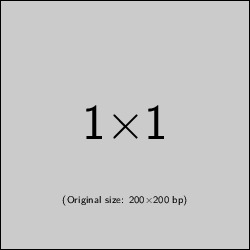
\includegraphics{example-image-1x1}%
      }%
    \end{captionbeside}
    \label{fig:maincls.captionbesidetop}
  \end{figure}
  \end{document}
\end{lstcode}
  \begin{figure}
    \KOMAoption{captions}{topbeside}
    \begin{captionbeside}[Beispiel: Bildbeschreibung daneben, oben]%
      {Eine Bildbeschreibung weder �ber noch unter der Abbildung,
        sondern oben daneben}[i][\linewidth]
      \raisebox{\dimexpr\baselineskip-\totalheight}{%
        \fbox{%
          \parbox[b][5\baselineskip][c]{.25\textwidth}{%
            \hspace*{\fill}\KOMAScript\hspace*{\fill}\par}}%
      }%
    \end{captionbeside}
    \label{fig:maincls.captionbesidetop}
  \end{figure}
\end{Example}
%
\EndIndexGroup


\begin{Declaration}
  \begin{Environment}{captionofbeside}
    \Parameter{Objekttyp}
    \OParameter{Verzeichnistitel}
    \Parameter{Titel}
    \OParameter{Anordnung}
    \OParameter{Breite}
    \OParameter{Offset}
    \begin{Body}\BodyDots\end{Body}
  \end{Environment}
  \labelsuffix[*]
  \begin{Environment}{captionofbeside}
    \Parameter{Objekttyp}
    \OParameter{Verzeichnistitel}
    \Parameter{Titel}
    \OParameter{Anordnung}
    \OParameter{Breite}
    \OParameter{Offset}\PValue{*}
    \begin{Body}\BodyDots\end{Body}
  \end{Environment}
\end{Declaration}
Wie\ChangedAt{v3.10}{\Class{scrbook}\and \Class{scrreprt}\and
  \Class{scrartcl}} zu \DescRef{\LabelBase.cmd.caption} mit
\DescRef{\LabelBase.cmd.captionof} eine Variante existiert, bei der der
\PName{Objekttyp} nicht durch die Verwendung innerhalb einer Gleitumgebung
dieses Typs bestimmt wird, so gibt es passend zur Umgebung
\DescRef{\LabelBase.env.captionbeside} mit \Environment{captionofbeside} auch
eine entsprechende Umgebung. Im Unterschied zu
\DescRef{\LabelBase.env.captionbeside} ist auch hier der \PName{Objekttyp} als
zus�tzliches, erstes Argument anzugeben.%
%
\EndIndexGroup

\begin{Declaration}
  \FloatStyle{komaabove}
  \FloatStyle{komabelow}
\end{Declaration}%
Bei\OnlyAt{\Package{float}} Verwendung des
\Package{float}-Pakets\IndexPackage{float} wird das Aussehen der damit
definierten Gleitumgebungen allein vom \emph{float}-Stil bestimmt. Dies
schlie�t auch die Frage ein, ob mit �berschriften oder Unterschriften
gearbeitet wird. Im \Package{float}-Paket gibt es keinen vordefinierten Stil,
der im Aussehen dem von \KOMAScript{} entspricht und dieselben
Einstellm�glichkeiten (siehe unten) bietet. \KOMAScript{} definiert deshalb
zus�tzlich die beiden Stile \PValue{komaabove} und \PValue{komabelow}. Diese
k�nnen bei Verwendung des \Package{float}-Pakets wie die dort definierten
Stile \PValue{plain}\IndexFloatstyle{plain},
\PValue{boxed}\IndexFloatstyle{boxed} oder
\PValue{ruled}\IndexFloatstyle{ruled} aktiviert werden. Siehe dazu
\cite{package:float}. Beim Stil \PValue{komaabove} werden \DescRef{\LabelBase.cmd.caption},
\DescRef{\LabelBase.cmd.captionabove} und \DescRef{\LabelBase.cmd.captionbelow} als �berschrift, beim Stil
\PValue{komabelow} als Unterschrift gesetzt.%
%
\EndIndexGroup


\begin{Declaration}
  \Macro{captionformat}
\end{Declaration}%
Bei {\KOMAScript} gibt es verschiedene Eingriffsm�glichkeiten, um die
Formatierung der Beschreibung zu �ndern. Die �nderung der Schriftart
wurde bereits erl�utert. Das oder die Trennzeichen zwischen dem Label
und dem eigentlichen Beschreibungstext sind im Makro
\Macro{captionformat} abgelegt.  Abweichend von allen anderen
\Macro{\dots}format-Anweisungen ist hier also nicht der Z�hler,
sondern nur die auf den Z�hler folgenden Angaben enthalten. Die
Originaldefinition lautet:
\begin{lstcode}
  \newcommand*{\captionformat}{:\ }
\end{lstcode}
Auch diese kann mit \Macro{renewcommand} ge�ndert werden.
\begin{Example}
  Aus mir unerfindlichen Gr�nden wollen Sie als Trennzeichen
  keinen Doppelpunkt gefolgt von einem Leerzeichen, sondern einen
  Gedankenstrich einschlie�lich der notwendigen Leerzeichen.
  Daher definieren Sie:
\begin{lstcode}
  \renewcommand*{\captionformat}{~--~}
\end{lstcode}
  Diese Definition sollten Sie beispielsweise in die Pr�ambel Ihres
  Dokuments stellen.
\end{Example}
%
\EndIndexGroup


\begin{Declaration}
  \Macro{figureformat}
  \Macro{tableformat}
\end{Declaration}%
Es wurde schon darauf hingewiesen, dass \DescRef{\LabelBase.cmd.captionformat}
keine Formatierung f�r das Label selbst enth�lt. Dieses sollte nun keineswegs
�ber Umdefinierung der Anweisungen f�r die Z�hlerausgabe, \Macro{thefigure}
oder \Macro{thetable}, ver�ndert werden. Eine solche Umdefinierung h�tte
n�mlich auch Auswirkungen auf die Ausgabe von \Macro{ref} oder der
Verzeichnisse. Stattdessen bietet {\KOMAScript} auch hier zwei \Macro{\dots
  format}-Anweisungen. Diese sind wie folgt vordefiniert:
% Umbruchkorrektur: listings
\begin{lstcode}
  \newcommand*{\figureformat}{\figurename~\thefigure\autodot}
  \newcommand*{\tableformat}{\tablename~\thetable\autodot}
\end{lstcode}
Sie k�nnen ebenfalls mit \Macro{renewcommand} eigenen Anforderungen
angepasst werden.
\begin{Example}
  Hin und wieder wird gew�nscht, dass die Beschreibungstexte ganz ohne
  Label und nat�rlich auch ohne Trennzeichen ausgegeben werden. Bei
  {\KOMAScript} gen�gen folgende Definitionen, um dies zu erreichen:
\begin{lstcode}
  \renewcommand*{\figureformat}{}
  \renewcommand*{\tableformat}{}
  \renewcommand*{\captionformat}{}
\end{lstcode}
  Dabei ist jedoch zu beachten, dass die Nummerierung damit zwar nicht
  ausgegeben, aber dennoch fortgez�hlt wird. Dies ist insbesondere dann
  von Bedeutung, wenn die Umdefinierungen nur auf einzelne
  \Environment{figure}- oder \Environment{table}-Umgebungen angewendet
  werden.
\end{Example}
%
\EndIndexGroup


\begin{Declaration}
  \Macro{setcapindent}\Parameter{Einzug}
  \Macro{setcapindent*}\Parameter{XEinzug}
  \Macro{setcaphanging}
\end{Declaration}%
Wie bereits erw�hnt wurde, werden in den
Standardklassen\textnote{\KOMAScript{} vs. Standardklassen} die
Beschreibungen nicht h�ngend gesetzt. Das hei�t: In mehrzeiligen
Beschreibungen beginnt die zweite Zeile direkt unter dem Labeltext.
Es gibt bei den Standardklassen auch keinen Mechanismus, dies direkt
zu beeinflussen. Bei {\KOMAScript} werden hingegen alle Zeilen ab der
zweiten so weit einger�ckt, dass diese nicht mehr unter dem Label,
�Abbildung~\dots:� oder �Tabelle~\dots:�, sondern unter dem
eigentlichen Text der ersten Zeile beginnen.

Dieses Verhalten, das der Verwendung von \Macro{setcaphanging}
entspricht, kann bei {\KOMAScript} jederzeit durch Verwendung der Anweisung
\Macro{setcapindent} oder \Macro{setcapindent*} ge�ndert werden. Dabei gibt
der Parameter \PName{Einzug} an, wie weit ab der zweiten Zeile einger�ckt
werden soll.  Soll nach dem Label und vor dem Beschreibungstext noch ein
Zeilenumbruch erfolgen, so definieren Sie die Einr�cktiefe \PName{XEinzug} der
Beschreibung stattdessen mit der Sternvariante der Anweisung:
\Macro{setcapindent*}.
Mit einem negativen \PName{Einzug} erreicht man hingegen, dass vor der
Beschreibung ebenfalls ein Umbruch erfolgt und nur die erste Zeile der
Beschreibung, nicht jedoch die folgenden, um den Betrag von \PName{Einzug}
einger�ckt werden.

Ob einzeilige Beschreibungen wie mehrzeilige Beschreibungen gesetzt werden
oder eine Sonderbehandlung erfahren, wird �ber die Option
\DescRef{\LabelBase.option.captions} gew�hlt. Siehe hierzu die Erkl�rung zu
den Werten \PValue{oneline} und \PValue{nooneline} dieser Option auf
\DescPageRef{\LabelBase.option.captions.oneline}.

\begin{Example}
  Die Abbildungen~\ref{fig:maincls.caption.first} bis
  \ref{fig:maincls.caption.last} zeigen die Auswirkungen unterschiedlicher
  Einstellungen. Dabei wird deutlich, dass bei geringer Spaltenbreite der
  komplett h�ngende Einzug unvorteilhaft ist. Der Quelltext der zweiten
  Abbildung sei hier mit abgewandelter Unterschrift beispielhaft
  wiedergegeben:
\begin{lstcode}
  \begin{figure}
    \setcapindent{1em}
    \fbox{\parbox{.95\linewidth}{%
        \centering\KOMAScript}}
    \caption{Beispiel mit teilweise h�ngendem Einzug 
      ab der zweiten Zeile}
  \end{figure}
\end{lstcode}
  Wie zu sehen ist, kann die Formatierung also auch lokal innerhalb
  der \Environment{figure}-Umgebung\IndexEnv{figure} ge�ndert werden. Die
  �nderung gilt dann nur f�r die eine Abbildung. Nachfolgende Abbildungen
  werden wieder mit den Grundeinstellungen oder den globalen Einstellungen,
  die Sie beispielsweise in der Dokumentpr�ambel vorgenommen haben,
  gesetzt. Das gilt f�r Tabellen nat�rlich genauso.
  \begin{figure}
    \typeout{^^J--- Ignore underfull and overfull \string\hbox:}
    \addtokomafont{caption}{\small}
    \addtokomafont{captionlabel}{\bfseries}
    \centering%
    \begin{minipage}{.92\linewidth}
      \begin{minipage}[t]{.48\linewidth}\sloppy
        \fbox{\parbox{.95\linewidth}{\centering{\KOMAScript}}}
        \caption[Beispiel: Bildunterschrift mit Voreinstellung]%
        {Mit der Stan\-dard\-ein\-stel\-lung, also wie bei
          Verwendung von \Macro{setcaphanging}}
        \label{fig:maincls.caption.first}
      \end{minipage}
      \hspace{.02\linewidth}
      \begin{minipage}[t]{.48\linewidth}\sloppy
        \setcapindent{1em}
        \fbox{\parbox{.95\linewidth}{\centering{\KOMAScript}}}
        \caption[Beispiel: Bildunterschrift mit teilweise h�ngendem Einzug]%
        {Mit teilweise h�ng"-endem Einzug ab der zweiten Zeile durch
          Verwendung von \Macro{setcapindent}\PParameter{1em}}
      \end{minipage}
    \end{minipage}

    \vspace*{2ex}\noindent%
    \begin{minipage}{.9\linewidth}
      \begin{minipage}[t]{.48\linewidth}\sloppy
        \setcapindent*{1em}
        \fbox{\parbox{.95\linewidth}{\centering{\KOMAScript}}}
        \caption[Beispiel: Bildunterschrift mit h�ngendem Einzug und Umbruch]%
        {Mit h�ngendem Einzug ab der zweiten Zeile und Umbruch vor
          der Beschreibung durch Verwendung von
          \Macro{setcapindent*}\PParameter{1em}}
      \end{minipage}
      \hspace{.02\linewidth}
      \begin{minipage}[t]{.48\linewidth}\sloppy
        \setcapindent{-1em}
        \fbox{\parbox{.95\linewidth}{\centering{\KOMAScript}}}
        \caption[Beispiel: Bildunterschrift mit Einzug in der zweiten Zeile]%
        {Mit Einzug lediglich in der zweiten Zeile und einem Umbruch
          vor der Beschreibung durch Verwendung von
          \Macro{setcapindent}\PParameter{-1em}}
                \label{fig:maincls.caption.last}
      \end{minipage}
    \end{minipage}
    \typeout{^^J--- Don't ignore underfull and overfull
      \string\hbox:^^J}
  \end{figure}
\end{Example}
%
\EndIndexGroup


\begin{Declaration}
  \Macro{setcapwidth}\OParameter{Ausrichtung}\Parameter{Breite}
  \Macro{setcapdynwidth}\OParameter{Ausrichtung}\Parameter{Breite}
  \Macro{setcapmargin}\OParameter{Rand \kern-.25em links}\Parameter{Rand}
  \Macro{setcapmargin*}\OParameter{Rand \kern-.25em innen}\Parameter{Rand}
\end{Declaration}
Mit \ChangedAt{v2.8q}{\Class{scrbook}\and \Class{scrreprt}\and
  \Class{scrartcl}} Hilfe dieser drei Befehle kann die Breite und Anordnung
der Beschreibung beeinflusst werden. Normalerweise steht die gesamte Text-
oder Spaltenbreite f�r den Text der Beschreibung zur Verf�gung.

Mit\important{\Macro{setcapwidth}} der Anweisung \Macro{setcapwidth} kann
diese \PName{Breite} reduziert werden. Dabei gibt das obligatorische Argument
die maximale f�r die Beschreibung verwendete \PName{Breite} an. Als optionales
Argument kann genau ein Buchstabe �bergeben werden, der die horizontale
Ausrichtung der Beschreibung angibt. Die m�glichen Ausrichtungen finden Sie in
der folgenden Liste.
\begin{labeling}[~--]{\quad\PValue{o}}\rightskip=1em
\item[\quad\PValue{l}] linksb�ndig
\item[\quad\PValue{c}] zentriert
\item[\quad\PValue{r}] rechtsb�ndig
\item[\quad\PValue{i}] innen: auf rechten Seiten linksb�ndig, auf
  linken Seiten rechtsb�ndig
\item[\quad\PValue{o}] au�en: auf rechten Seiten rechtsb�ndig, auf
  linken Seiten linksb�ndig
\end{labeling}
Die Ausrichtung innen und au�en entspricht im einseitigen Satz linksb�ndig und
rechtsb�ndig. Innerhalb\textnote{Achtung!} von
\Package{longtable}\IndexPackage{longtable}-Tabellen%
\important{\Package{longtable}} funktioniert die Ausrichtung innen und au�en
nicht korrekt. Insbesondere werden Beschreibungen von Folgeseiten bei diesen
Tabellen immer nach den Beschreibungen der ersten Teiltabelle
ausgerichtet. Dies ist ein konzeptionelles Problem des Paketes
\Package{longtable}.

Zu\ChangedAt{v3.20}{\Class{scrbook}\and \Class{scrreprt}\and
  \Class{scrartcl}}\textnote{Achtung!} beachten ist, dass die an
\Macro{setcapwidth} �bergebene \PName{Breite} wie bei \Macro{setlength} zum
Zeitpunkt der Zuweisung ausgewertet wird. Will man hingegen, dass
\PName{Breite} erst bei der Verwendung ausgewertet wird, dann sollte man
stattdessen \Macro{setcapdynwidth} verwenden. Entscheidende Unterschiede gibt
es beispielsweise, wenn L�ngen wie \Length{linewidth} oder andere Anweisungen
als Argument verwendet werden.

Mit\important{\Macro{setcapmargin}} der Anweisung \Macro{setcapmargin} kann
statt der Breite der Beschreibung ein \PName{Rand} angegeben werden, der neben
der Beschreibung zus�tzlich zum normalen Textrand eingehalten werden soll.
Sollen der Rand rechts und links nicht identisch gew�hlt werden, kann mit dem
optionalen Argument ein von \PName{Rand} abweichender \PName{Rand \kern-.25em
  links} von der Beschreibung eingestellt
werden. Bei\important{\Macro{setcapmargin*}} der Sternvariante
\Macro{setcapmargin*} wird statt \PName{Rand \kern-.25em links} im
doppelseitigen Satz \PName{Rand \kern-.25em innen} abweichend definiert.
Hier\textnote{Achtung!} ergibt sich bei
\Package{longtable}\IndexPackage{longtable}-Tabellen%
\important{\Package{longtable}} das gleiche Problem wie bei der Ausrichtung
au�en oder innen bei der Anweisung \Macro{setcapwidth}. Die Verwendung von
\Macro{setcapmargin} oder \Macro{setcapmargin*} aktiviert au�erdem
\OptionValueRef{\LabelBase}{captions}{nooneline} (siehe
\DescPageRef{\LabelBase.option.captions.nooneline}) f�r die Beschreibungen,
die mit dieser Randeinstellung gesetzt werden.

Man\textnote{Tipp!} kann �brigens auch negative Werte f�r \PName{Rand} und
\PName{Rand \kern-.25em rechts} oder \PName{Rand \kern-.25em au�en}
angeben. Dadurch erreicht man, dass die Beschreibung in den entsprechenden
Rand hineinragt.

F�r\textnote{Tipp!} Experten und versierte Anwender ist eine etwas
trickreiche Anwendung f�r \Macro{setcapwidth} in
\iffree{\cite{book:komascript}}{\autoref{cha:floattricks},
  \autopageref{cha:floattricks}} zu finden.%
%
\EndIndexGroup


\begin{Declaration}
  \Option{origlongtable}
\end{Declaration}%
\BeginIndex{Package}{longtable}%
Falls die Tabellen�berschriften des \Package{longtable}-Pakets (siehe
\cite{package:longtable}) von den \KOMAScript-Klassen nicht umdefiniert werden
sollen, kann die Option \Option{origlongtable} gesetzt werden. Diese
Option\textnote{Achtung!}  ist als optionales Argument von
\DescRef{\LabelBase.cmd.documentclass} zu verwenden. Eine Einstellung per
\DescRef{\LabelBase.cmd.KOMAoptions} oder \DescRef{\LabelBase.cmd.KOMAoption}
wird nicht unterst�tzt.
%
\EndIndexGroup
%
\EndIndexGroup


\begin{Declaration}
  \OptionVName{listof}{Einstellung}
\end{Declaration}
Normalerweise\ChangedAt{v3.00}{\Class{scrbook}\and \Class{scrreprt}\and
  \Class{scrartcl}} werden die Verzeichnisse der Gleitumgebungen -- wie das
Tabellen"~\Index{Tabellen>Verzeichnis} und das
Abbildungsverzeichnis\Index{Abbildungen>Verzeichnis} -- nicht nummeriert oder
in das Inhaltsverzeichnis aufgenommen. In \autoref{sec:\LabelBase.toc} wurde
dies bereits n�her ausgef�hrt. Alternativ zu den dort erw�hnten Einstellungen
\OptionValueRef{\LabelBase}{toc}{nolistof}%
\IndexOption{toc~=\PValue{nolistof}},
\OptionValueRef{\LabelBase}{toc}{listof}\IndexOption{toc~=\PValue{listof}} und
\OptionValueRef{\LabelBase}{toc}{listofnumbered}%
\IndexOption{toc~=\PValue{listofnumbered}}, kann dieses Verhalten auch aus
Sicht der Verzeichnisse selbst gesehen werden. Daher kann man die gleichen
Ergebnisse auch mit den Einstellungen \OptionValue{listof}{notoc},
\OptionValue{listof}{totoc} und \OptionValue{listof}{numbered} erreichen.

Dabei werden in der Voreinstellung f�r die �berschriften der Verzeichnisse die
oberste verf�gbare Gliederungsebene unterhalb von
\DescRef{\LabelBase.cmd.part} verwendet. Bei \Class{scrbook} und
\Class{scrreprt} ist das die Kapitelebene, bei \Class{scrartcl} die
Abschnittsebene. Mit\important{\OptionValue{listof}{leveldown}}%
\ChangedAt{v3.06}{\Class{scrbook}\and \Class{scrreprt}\and \Class{scrartcl}}
Hilfe der Einstellung \OptionValue{listof}{leveldown} kann hingegen die n�chst
tiefere Gliederungsebene verwendet werden.
\begin{Example}
  Sie wollen in einem Buch das Abbildungs- und das Tabellenverzeichnis als
  Unterverzeichnisse eines gemeinsamen Verzeichnisses �Abbildungen und
  Tabellen� setzen. Dazu verwenden Sie einfach:
\begin{lstcode}
  \KOMAoption{listof}{leveldown}
\end{lstcode}
  und dann an entsprechender Stelle Ihres Dokuments:
\begin{lstcode}
  \addchap*{Abbildungs- und Tabellenverzeichnis}
  \listoffigures
  \listoftables
\end{lstcode}
  N�heres zur Anweisung \DescRef{\LabelBase.cmd.addchap*} ist
  \autoref{sec:\LabelBase.structure}, \DescPageRef{\LabelBase.cmd.addchap*} zu
  entnehmen.
\end{Example}

Normalerweise\ChangedAt{v2.8q}{%
  \Class{scrbook}\and \Class{scrreprt}\and \Class{scrartcl}} werden die
Verzeichnisse\Index{Abbildungen>Verzeichnis}\Index{Tabellen>Verzeichnis}
der Gleitumgebungen so formatiert, dass f�r die Nummer ein Raum fester Breite
verwendet wird. Gleichzeitig werden alle Eintr�ge leicht eingezogen. Dies
entspricht der Verwendung der Einstellung
\OptionValue{listof}{graduated}\IndexOption{listof~=\PValue{graduated}}.

Werden die Nummern sehr breit, weil beispielsweise sehr viele Tabellen
verwendet werden, so reicht der vorgesehene Platz irgendwann nicht mehr aus.
Vergleichbar\important{\OptionValue{listof}{flat}} zur Einstellung
\OptionValueRef{\LabelBase}{toc}{flat}\IndexOption{toc~=\PValue{flat}} f�r das
Inhaltsverzeichnis bietet \KOMAScript{} daher die Einstellung
\OptionValue{listof}{flat}\IndexOption{listof~=\PValue{flat}} f�r die
Verzeichnisse der Gleitumgebungen. Dabei wird die Breite der Nummern
automatisch ermittelt und der Platz entsprechend angepasst. Bez�glich der
Nebenwirkungen und Funktionsweise gilt, was in \autoref{sec:\LabelBase.toc},
\DescPageRef{\LabelBase.option.toc.flat} f�r die Einstellung
\OptionValueRef{\LabelBase}{toc}{flat} erkl�rt wurde. Es sei an dieser Stelle
jedoch nochmals darauf hingewiesen, dass mit der Einstellung
\OptionValue{listof}{flat} mehrere \LaTeX-Durchl�ufe ben�tigt werden, bis die
Verzeichnisse ihre endg�ltige Form erhalten haben.

Die Einstellung \OptionValue{listof}{flat} wird automatisch aktiviert, falls
die Einstellung
\OptionValue{listof}{entryprefix}\ChangedAt{v3.06}{\Class{scrbook}\and
  \Class{scrreprt}\and \Class{scrartcl}} verwendet
wird. Normalerweise\important{\OptionValue{listof}{entryprefix}} ist es nicht
sinnvoll jeden Eintrag in eines der Verzeichnisse der Gleitumgebungen mit
einem Pr�fix wie �Abbildung� oder �Tabelle� zu versenden, da nat�rlich im
Abbildungsverzeichnis nur Abbildungen und im Tabellenverzeichnis nur Tabellen
zu finden sind. Damit hat ein solcher Pr�fix keinen zus�tzlichen
Informationswert und wird in der Voreinstellung auch weggelassen. Mit der
Einstellung \OptionValue{listof}{entryprefix} wird ein solcher Pr�fix jedoch
gesetzt. Dabei erhalten alle Eintr�ge eines Verzeichnisses denselben
Pr�fix. Dieser richtet sich nach dem Dateianhang der Hilfsdatei, die f�r das
Verzeichnis verwendet wird. F�r das Abbildungsverzeichnis, das den Dateianhang
�\File{lof}� besitzt, wird beispielsweise \Macro{listoflofentryname} verwendet,
w�hrend f�r das Tabellenverzeichnis, das den Dateianhang �\File{lot}� besitzt,
\Macro{listoflotentryname} verwendet wird.

Bei den Klassen \Class{scrbook} und
\Class{scrreprt}\OnlyAt{\Class{scrbook}\and \Class{scrreprt}} f�gt
\KOMAScript{} in der Voreinstellung bei jedem Kapitelanfang einen vertikalen
Abstand in die Verzeichnisse der Gleitumgebungen ein. Dieses Verhalten, das es
auch bei den Standardklassen gibt, dient dazu, diese Verzeichnisse nach
Kapiteln zu gruppieren. Es entspricht bei \KOMAScript{} der
Einstellung\ChangedAt{v3.00}{\Class{scrbook}\and \Class{scrreprt}\and
  \Class{scrartcl}} \OptionValue{listof}{chaptergapsmall}%
\IndexOption{listof~=\PValue{chaptergapsmall}}.  Dabei wird ein fester
vertikaler Abstand von 10\Unit{pt}
verwendet. Mit\important{\OptionValue{listof}{chaptergapline}} der Einstellung
\OptionValue{listof}{chaptergapline}%
\IndexOption{listof~=\PValue{chaptergapline}} kann man stattdessen einen
vertikalen Abstand von einer Zeile
erreichen. Mit\important{\OptionValue{listof}{nochaptergap}}
\OptionValue{listof}{nochaptergap}\IndexOption{listof~=\PValue{nochaptergap}}
kann man den vertikalen Abstand komplett
abschalten. Eine\important{\OptionValue{listof}{chapterentry}} Besonderheit
stellt die Einstellung
\OptionValue{listof}{chapterentry}\IndexOption{listof~=\PValue{chapterentry}}
dar. Dabei wird statt des Abstandes der Inhaltsverzeichniseintrag f�r das
Kapitel in das Verzeichnis der Gleitumgebungen
eingef�gt. Es\textnote{Achtung!} wird darauf hingewiesen, dass ein solcher
Eintrag auch dann erfolgt, wenn das Kapitel keine Gleitumgebung enth�lt. Eine
noch direktere Beeinflussung, was in den Verzeichnissen der Gleitumgebungen
bei neuen Kapiteln geschehen soll, ist mit der Option
\DescRef{\LabelBase.option.chapteratlists} zu erreichen, die in
\autoref{sec:\LabelBase.structure} auf
\DescPageRef{\LabelBase.option.chapteratlists} erl�utert wird.

Einen �berblick �ber alle m�glichen Werte f�r die \PName{Einstellung} von
\Option{listof} ist in \autoref{tab:maincls.listof} zu finden.

\begin{desclist}
  \desccaption[{M�gliche Werte f�r Option \Option{listof}}]{%
    M�gliche Werte f�r Option \Option{listof} zur Einstellung von Form und
    Inhalt der Verzeichnisse der Gleitumgebungen\label{tab:maincls.listof}%
  }{%
    M�gliche Werte f�r Option \Option{listof} (\emph{Fortsetzung})%
  }%
  \entry{\PValue{chapterentry}, \PValue{withchapterentry}}{%
    Kapitelanf�nge werden in den Verzeichnissen der Gleitumgebungen durch
    einen Inhaltsverzeichniseintrag des Kapitels markiert.%
    \IndexOption{listof~=\PValue{chapterentry}}}%
  \entry{\PValue{chaptergapline}, \PValue{onelinechaptergap}}{%
    Kapitelanf�nge werden in den Verzeichnissen der Gleitumgebungen durch
    einen Abstand von einer Zeile markiert.%
    \IndexOption{listof~=\PValue{chaptergapline}}}%
  \entry{\PValue{chaptergapsmall}, \PValue{smallchaptergap}}{%
    Kapitelanf�nge werden in den Verzeichnissen der Gleitumgebungen durch
    einen kleinen Abstand markiert.%
    \IndexOption{listof~=\PValue{chaptergapsmall}}}%
  \entry{\PValue{entryprefix}}{%
    \ChangedAt{v3.06}{\Class{scrbook}\and \Class{scrreprt}\and
      \Class{scrartcl}}%
    Jeder Verzeichniseintrag wird mit einem vom Verzeichnis abh�ngenden Pr�fix
    vor der Nummer versehen. Der Pr�fix ist normalerweise sprachabh�ngig,
    beispielsweise bei deutschen Spracheinstellungen �Abbildung� f�r das
    Abbildungsverzeichnis und �Tabelle� f�r das Tabellenverzeichnis jeweils
    gefolgt von einem Leerzeichen.%
    \IndexOption{listof~=\PValue{entryprefix}}}%
  \entry{\PValue{flat}, \PValue{left}}{%
    Die Verzeichnisse der Gleitumgebungen erhalten eine tabellarische
    Form. Die Gleitumgebungsnummern sind dabei die erste Spalte, der Titel die
    zweite Spalte, die Seitenzahlen die dritte Spalte. Der Platz, der f�r die
    Gleitumgebungsnummern reserviert wird, richtet sich nach dem ben�tigten
    Platz des vorherigen \LaTeX-Laufs.%
    \IndexOption{listof~=\PValue{flat}}}%
  \entry{\PValue{graduated}, \PValue{indent}, \PValue{indented}}{%
    Die Verzeichnisse der Gleitumgebungen erhalten eine hierarchische Form. Es
    steht nur ein begrenzter Platz f�r die Gleitumgebungsnummern zur
    Verf�gung.%
    \IndexOption{listof~=\PValue{graduated}}}%
  \entry{\PValue{indenttextentries}, \PValue{indentunnumbered},
    \PValue{numberline}}{%
    \ChangedAt{v3.12}{\Class{scrbook}\and \Class{scrreprt}\and
      \Class{scrartcl}}%
    Die Eigenschaft \PValue{numberline} (siehe \autoref{sec:tocbasic.toc},
    \DescPageRef{tocbasic.cmd.setuptoc}) wird f�r die Verzeichnisse der
    Gleitumgebungen, beispielsweise das Abbildungs"~ und das
    Tabellenverzeichnis, gesetzt. Dadurch werden nicht nummerierte Eintr�ge
    linksb�ndig mit dem Text von nummerierten Eintr�gen gleicher Ebene
    gesetzt. Allerdings bieten die \KOMAScript-Klassen selbst keine nicht
    nummerierten Eintr�ge in diese Verzeichnisse. Dies hat daher nur
    Auswirkungen auf entsprechende Eintr�ge, die nicht von den Klassen selbst,
    aber dennoch mit Hilfe von \DescRef{tocbasic.cmd.addxcontentsline} (siehe
    \autoref{sec:tocbasic.toc}, \DescPageRef{tocbasic.cmd.addxcontentsline})
    erzeugt werden.%
    \IndexOption{toc~=\PValue{numberline}}}%
  \entry{\PValue{leftaligntextentries}, \PValue{leftalignunnumbered},
    \PValue{nonumberline}}{%
    \ChangedAt{v3.12}{\Class{scrbook}\and \Class{scrreprt}\and
      \Class{scrartcl}}%
    Die Eigenschaft \PValue{numberline} (siehe \autoref{sec:tocbasic.toc},
    \DescPageRef{tocbasic.cmd.setuptoc}) wird f�r die Verzeichnisse der
    Gleitumgebungen, beispielsweise das Abbildungs"~ und das
    Tabellenverzeichnis, gesetzt. Dadurch werden nicht nummerierte Eintr�ge
    linksb�ndig mit der Nummer von nummerierten Eintr�gen gleicher Ebene
    gesetzt. Allerdings bieten die \KOMAScript-Klassen selbst keine nicht
    nummerierten Eintr�ge in diese Verzeichnisse. Dies hat daher nur
    Auswirkungen auf entsprechende Eintr�ge, die nicht von den Klassen selbst,
    aber dennoch mit Hilfe von \DescRef{tocbasic.cmd.addxcontentsline} (siehe
    \autoref{sec:tocbasic.toc}, \DescPageRef{tocbasic.cmd.addxcontentsline})
    erzeugt werden.%
    \IndexOption{toc~=\PValue{numberline}}}%
  \entry{\PValue{leveldown}}{%
    Die Verzeichnisse werden um eine Gliederungsebene nach unten verschoben.%
    \IndexOption{listof~=\PValue{leveldown}}}%
  \entry{\PValue{nochaptergap}, \PValue{ignorechapter}}{%
    Kapitelanf�nge werden in den Verzeichnissen der Gleitumgebungen nicht
    markiert.%
    \IndexOption{listof~=\PValue{nochaptergap}}}%
  \entry{\PValue{notoc}, \PValue{plainheading}}{%
    Die Verzeichnisse der Gleitumgebungen, beispielsweise das Abbildungs"~ und
    das Tabellenverzeichnis, erhalten keinen Eintrag im Inhaltsverzeichnis.%
    \IndexOption{listof~=\PValue{notoc}}}%
  \entry{\PValue{numbered}, \PValue{totocnumbered}, \PValue{tocnumbered},
    \PValue{numberedtotoc}}{%
    Die Verzeichnisse der Gleitumgebungen, beispielsweise das Abbildungs"~ und
    das Tabellenverzeichnis, erhalten einen Eintrag im Inhaltsverzeichnis und
    werden nummeriert.%
    \IndexOption{listof~=\PValue{numbered}}}%
  \entry{\PValue{totoc}, \PValue{toc}, \PValue{notnumbered}}{%
    Die Verzeichnisse der Gleitumgebungen, beispielsweise das Abbildungs"~ und
    das Tabellenverzeichnis, erhalten einen Eintrag im Inhaltsverzeichnis,
    ohne dass sie nummeriert werden.%
    \IndexOption{listof~=\PValue{totoc}}}%
\end{desclist}
%
\EndIndexGroup


\begin{Declaration}
  \Macro{listoftables}
  \Macro{listoffigures}
\end{Declaration}%
Mit diesen Anweisungen kann ein Verzeichnis der Tabellen beziehungsweise der
Abbildungen ausgegeben werden. �nderungen, die Auswirkungen auf diese
Verzeichnisse haben, werden erst nach zwei \LaTeX{}-L�ufen sichtbar. Die Form
der Verzeichnisse kann durch die Option
\DescRef{\LabelBase.option.listof}\important{\DescRef{\LabelBase.option.listof}}
mit den Werten \PValue{graduated} und \PValue{flat} beeinflusst werden (siehe
\DescPageRef{\LabelBase.option.listof}). Dar�ber hinaus wirken sich indirekt
die Werte \PValue{listof} und \PValue{listofnumbered} f�r die Option
\DescRef{\LabelBase.option.toc}\important{\DescRef{\LabelBase.option.toc}}
(siehe \autoref{sec:\LabelBase.toc}, \DescPageRef{\LabelBase.option.toc}),
sowie die Werte \PValue{totoc} und \PValue{totocnumbered} der oben erl�uterten
Option \DescRef{\LabelBase.option.listof} auf die Verzeichnisse aus.

In\textnote{Tipp!} der Regel findet man die Verzeichnisse der
Gleitumgebungen\Index{Gleitumgebungen}, also das 
\index{Tabellen>Verzeichnis}Tabellen- und das 
Abbildungsverzeichnis\index{Abbildungen>Verzeichnis}, unmittelbar nach dem
Inhaltsverzeichnis. In einigen Dokumenten wandern diese auch in den
Anhang. Der Autor bevorzugt jedoch die Platzierung unmittelbar nach dem
Inhaltsverzeichnis.%
%
\EndIndexGroup


\LoadCommonFile{marginpar}% \section{Randnotizen}


\section{Anhang}
\seclabel{appendix}
\BeginIndexGroup
\BeginIndex{}{Anhang}

Der Anhang eines Dokuments besteht im Wesentlichen aus den Anlagen zu einem
Dokument. Typische Teile eines Anhangs sind Literaturverzeichnis,
Stichwortverzeichnis und Begriffsverzeichnis. Alleine f�r diese Teile w�rde
man jedoch keinen Anhang beginnen, da diese Teile normalerweise schon von sich
aus eine Auszeichnung besitzen, die sie als Anhang erkennbar macht. Enth�lt
der Anhang aber weitere Teile wie beispielsweise zitierte Fremddokumente,
Endnoten oder Tafeln, so werden die zuvor genannten Teile ebenfalls im Anhang
gesetzt.


\begin{Declaration}
  \Macro{appendix}
\end{Declaration}%
Der Anhang wird in den Standardklassen und den {\KOMAScript}-Klassen mit der
Anweisung \Macro{appendix} eingeleitet. Diese Anweisung schaltet unter anderem
die Kapitelnummerierung auf Gro�buchstaben um und sorgt gleichzeitig daf�r,
dass die Regeln f�r die Nummerierung der Gliederungsebenen nach \cite{DUDEN}
eingehalten werden. Diese Regeln sind in der Beschreibung der Option
\DescRef{\LabelBase.option.numbers} in \autoref{sec:\LabelBase.structure},
\DescPageRef{\LabelBase.option.numbers} n�her erl�utert.

Die Form der Kapitel�berschriften\OnlyAt{\Class{scrbook}\and \Class{scrreprt}}
im Anhang wird durch die Optionen \DescRef{\LabelBase.option.chapterprefix}
und \DescRef{\LabelBase.option.appendixprefix} bestimmt. N�heres dazu ist
\autoref{sec:\LabelBase.structure},
\DescPageRef{\LabelBase.option.appendixprefix} zu entnehmen.

Bitte\textnote{Achtung!} beachten Sie, dass es sich bei \Macro{appendix} um
eine Anweisung und \emph{nicht} um eine Umgebung handelt! Die Anweisung
erwartet auch nicht etwa ein Argument. Die Kapitel beziehungsweise Abschnitte
des Anhangs werden ganz normal mit \DescRef{\LabelBase.cmd.chapter} und
\DescRef{\LabelBase.cmd.section} gesetzt.%
%
\EndIndexGroup
%
\EndIndexGroup


\section{Literaturverzeichnis}
\seclabel{bibliography}
\BeginIndexGroup
\BeginIndex{}{Literaturverzeichnis}

Das Literaturverzeichnis erschlie�t externe Quellen. In der Regel wird das
Literaturverzeichnis mit Hilfe des Programms \BibTeX{} aus einer Datei mit
datenbank�hnlicher Struktur erzeugt. Dabei kann �ber den \BibTeX-Stil sowohl
die Form der Eintr�ge als auch deren Sortierung ver�ndert werden. Wird
zus�tzlich ein Literaturpaket, beispielsweise
\Package{natbib}\IndexPackage{natbib},
\Package{babelbib}\IndexPackage{babelbib} oder
\Package{biblatex}\IndexPackage{biblatex} verwendet, so schwindet der Einfluss
von \KOMAScript{} auf das Literaturverzeichnis. In diesen F�llen ist unbedingt
die Anleitung des verwendeten Pakets zu beachten! Zur generellen Verwendung
eines Literaturverzeichnisses sei auf \cite{l2kurz} verwiesen.


\begin{Declaration}
  \OptionVName{bibliography}{Einstellung}
\end{Declaration}
Als \PName{Einstellung}\ChangedAt{v3.00}{\Class{scrbook}\and
  \Class{scrreprt}\and \Class{scrartcl}} kann zun�chst einmal jeder definierte
Formatierungsstil gew�hlt werden. Vordefiniert sind bei \KOMAScript{} zwei
solche Formatierungsstile f�r das Literaturverzeichnis. Diese sind jedoch
nicht zu verwechseln mit den unterschiedlichen Stilen f�r
\BibTeX\Index{BibTeX=\BibTeX}, die man mit \Macro{bibstyle} ausw�hlt. W�hrend
\BibTeX{} sowohl die Art der Sortierung als auch den Inhalt des
Literaturverzeichnisses bestimmt, k�nnen �ber die Einstellungen von
\KOMAScript{} nur grundlegende Eigenschaften des Literaturverzeichnisses oder
einige wenige Eigenschaften der Formatierung der Eintr�ge beeinflusst werden.

Mit\important{\OptionValue{bibliography}{oldstyle}}
\OptionValue{bibliography}{oldstyle}%
\IndexOption{bibliography~=\PValue{oldstyle}} wird
die kompakte Formatierung gew�hlt. Dabei f�hrt die Anweisung
\DescRef{maincls-experts.cmd.newblock}\IndexCmd{newblock} in den einzelnen Eintr�gen lediglich zu
einem dehnbaren horizontalen Abstand. Der Name kommt daher, dass dies die
h�ufigste klassische Form eines Literaturverzeichnisses
ist. Demgegen�ber\important[i]{\begin{tabular}[t]{@{}l@{}}
      \Option{bibliography=}\\
      \quad\PValue{openstyle}\end{tabular}} erreicht
man die etwas modernere, offene Form mit der Einstellung
\OptionValue{bibliography}{openstyle}%
\IndexOption{bibliography~=\PValue{openstyle}}. Der
Name kommt daher, dass hier die Anweisung \DescRef{maincls-experts.cmd.newblock} einen Absatz
einf�gt. Die Eintr�ge im Literaturverzeichnis werden so st�rker
gegliedert. Sie sind weniger kompakt und deutlich aufgelockerter oder
ge�ffnet.  Bez�glich der M�glichkeit, neue Formatierungsstile zu definieren,
sei auf \DescRef{maincls-experts.cmd.newbibstyle}, \autoref{sec:maincls-experts.experts},
\DescPageRef{maincls-experts.cmd.newbibstyle} verwiesen.

Neben dem Formatierungsstil gibt es eine weitere Eigenschaft, die �ber
\PName{Einstellung} ver�ndert werden kann. Das Literaturverzeichnis stellt
eine Art von Verzeichnis dar, bei der nicht der Inhalt des vorliegenden Werks
aufgelistet, sondern auf externe Inhalte verwiesen
wird. Mit dieser Begr�ndung
k�nnte man argumentieren, dass das Literaturverzeichnis ein eigenes Kapitel
bzw. einen eigenen Abschnitt darstellt und somit eine
Nummer verdiene.  Die
Einstellung \OptionValue{bibliography}{totocnumbered}%
\important[i]{\begin{tabular}[t]{@{}l@{}}
    \Option{bibliography=}\\
    \quad\PValue{totocnumbered}
  \end{tabular}}\IndexOption{bibliography~=\PValue{totocnumbered}} f�hrt genau
dazu, einschlie�lich des dann f�lligen Eintrags im Inhaltsverzeichnis.  Ich
selbst bin der Meinung, dass bei dieser Argumentation auch ein klassisches,
kommentiertes Quellenverzeichnis ein eigenes Kapitel w�re. Au�erdem ist das
Literaturverzeichnis letztlich nichts, was man selbst geschrieben
hat. Deshalb\important{\OptionValue{bibliography}{totoc}}
verdient es allenfalls einen nicht nummerierten Eintrag im
Inhaltsverzeichnis, was mit der Einstellung
\OptionValue{bibliography}{totoc}\IndexOption{bibliography~=\PValue{totoc}}
erreicht wird. Die Voreinstellung, bei der das Literaturverzeichnis als nicht
nummeriertes Kapitel ohne eigenen Inhaltsverzeichniseintrag gesetzt wird,
entspricht \OptionValue{bibliography}{nottotoc}%
\IndexOption{bibliography~=\PValue{nottotoc}}. Siehe
hierzu auch Option \DescRef{\LabelBase.option.toc} in \autoref{sec:\LabelBase.toc},
insbesondere die Werte \PValue{bibliographynumbered}, \PValue{bibliography}
und \PValue{nobibliography} ab
\DescPageRef{\LabelBase.option.toc.bibliography}.

In\ChangedAt{v3.12}{\Class{scrbook}\and \Class{scrreprt}\and \Class{scrartcl}}
einigen F�llen wird nicht das gesamte Dokumente mit einem einzigen
Literaturverzeichnis versehen, sondern jedes Kapitel eines mit \Class{scrbook}
oder \Class{scrreprt} gesetzten Dokuments erh�lt sein eigenes
Literaturverzeichnis. In diesem Fall ist es sinnvoll,
wenn\important{\OptionValue{bibliography}{leveldown}} das Literaturverzeichnis
selbst nicht auf Kapitel, sondern etwas tiefer auf Abschnittsebene angesiedelt
wird. Dies ist mit Option \OptionValue{bibliography}{leveldown}%
\IndexOption{bibliography~=\PValue{leveldown}} zu erreichen. Diese kann
beispielsweise auch verwendet werden, wenn das Literaturverzeichnis zusammen
mit anderen Verzeichnissen unter einer gemeinsamen �berschrift erscheinen
soll. Daher ist diese Option auch in \Class{scrartcl} verf�gbar.

Eine Zusammenfassung m�glicher Werte f�r \PName{Einstellung} ist
\autoref{tab:maincls.bibliography} zu entnehmen. Es ist jedoch zu beachten,
dass mit \DescRef{maincls-experts.cmd.newbibstyle}\IndexCmd{newbibstyle}
weitere Werte definiert werden k�nnen.

\begin{table}
  \caption[{M�gliche Werte f�r Option \Option{bibliography}}]{Vordefinierte
    Werte f�r Option \Option{bibliography} zur Einstellung der Form des
    Literatur\-verzeichnisses}
  \label{tab:maincls.bibliography}
  \begin{desctabular}
    \pventry{leveldown}{%
      \ChangedAt{v3.12}{\Class{scrbook}\and \Class{scrreprt}\and
        \Class{scrartcl}}%
      Das Literaturverzeichnis wird um eine Gliederungsebene nach unten
      verschoben.%
      \IndexOption{bibliography~=\PValue{leveldown}}}%
    \pventry{nottotoc}{%
      Das Literaturverzeichnis erh�lt keinen Eintrag im Inhaltsverzeichnis und
      wird auch nicht nummeriert.%
      \IndexOption{bibliography~=\PValue{nottotoc}}}%
    \pventry{oldstyle}{%
      Es wird die klassische, kompakte Formatierung gew�hlt, bei der
      \DescRef{maincls-experts.cmd.newblock}\IndexCmd{newblock} nur einen
      dehnbaren horizontalen Abstand darstellt.%
      \IndexOption{bibliography~=\PValue{oldstyle}}}%
    \pventry{openstyle}{%
      Es wird eine untergliederte, offene Formatierung gew�hlt, bei der
      \DescRef{maincls-experts.cmd.newblock}\IndexCmd{newblock} einen Absatz
      darstellt.%
      \IndexOption{bibliography~=\PValue{openstyle}}}%
    \pventry{totoc}{%
      Das Literaturverzeichnis erh�lt einen Eintrag im Inhaltsverzeichnis,
      ohne dass es nummeriert wird.%
      \IndexOption{bibliography~=\PValue{totoc}}}%
    \pventry{totocnumbered}{%
      Das Literaturverzeichnis erh�lt einen Eintrag im Inhaltsverzeichnis und
      wird nummeriert.%
      \IndexOption{bibliography~=\PValue{totocnumbered}}}%
  \end{desctabular}
\end{table}
%
\EndIndexGroup


\begin{Declaration}
  \Macro{setbibpreamble}\Parameter{Pr�ambel}
\end{Declaration}%
Mit der Anweisung \Macro{setbibpreamble} kann eine Pr�ambel f�r das
Literaturverzeichnis gesetzt werden. Bedingung daf�r ist, dass die Pr�ambel
vor der Anweisung zum Setzen des Literaturverzeichnisses gesetzt wird. Dies
muss nicht unmittelbar davor sein. Es kann also beispielsweise am Anfang des
Dokuments erfolgen. Ebenso\textnote{Achtung!} wie Option
\OptionValue{bibliography}{totoc} oder
\OptionValue{bibliography}{totocnumbered} kann die Anweisung aber nur
erfolgreich sein, wenn nicht ein Paket geladen wird, das dies durch
Umdefinierung der \Environment{thebibliography}-Umgebung verhindert. Obwohl
das \Package{natbib}-Paket\IndexPackage{natbib} nicht freigegebene interne
Makros von {\KOMAScript} verwendet, konnte erreicht werden, dass
\Macro{setbibpreamble} auch mit der aktuellen Version von \Package{natbib}
funktioniert (siehe \cite{package:natbib}).
\begin{Example}
  Sie wollen darauf hinweisen, dass das Literaturverzeichnis nicht in
  der Reihenfolge der Zitierung im Dokument, sondern alphabetisch
  sortiert ist. Daher setzen Sie folgende Anweisung:
\begin{lstcode}
  \setbibpreamble{Die Literaturangaben sind 
    alphabetisch nach den Namen der Autoren 
    sortiert. Bei mehreren Autoren wird nach dem 
    ersten Autor sortiert.\par\bigskip}
\end{lstcode}
  Die Anweisung \Macro{bigskip}\IndexCmd{bigskip} sorgt daf�r, dass
  zwischen der Pr�ambel und der ersten Literaturangabe ein gro�er
  Zwischenraum gesetzt wird.%
\end{Example}
%
\EndIndexGroup


\begin{Declaration}
  \Macro{BreakBibliography}\Parameter{Unterbrechung}
\end{Declaration}
Diese\textnote{Achtung!}\ChangedAt{v3.00}{\Class{scrbook}\and
  \Class{scrreprt}\and \Class{scrartcl}} Anweisung existiert nur, wenn
Umgebung \Environment{thebibliography} nicht durch ein Paket neu definiert
wurde. In diesem Fall ist es m�glich, mit dieser Anweisung das
Literaturverzeichnis zu unterbrechen. Die \PName{Unterbrechung} wird dann
innerhalb einer Gruppe ausgegeben. Eine solche \PName{Unterbrechung} k�nnte
beispielsweise eine �berschrift mit Hilfe von \DescRef{\LabelBase.cmd.minisec}
sein. Leider gibt es bisher keine M�glichkeit, diese Anweisung beispielsweise
mit Hilfe eines speziellen Eintrags in der Literaturdatenbank von \BibTeX{}
erzeugen zu lassen. Daher kann sie derzeit nur von Anwendern verwendet werden,
die das Literaturverzeichnis selbst editieren. Ihr Nutzen ist damit sehr
beschr�nkt.%
%
\EndIndexGroup


\begin{Declaration}
  \Macro{AfterBibliographyPreamble}\Parameter{Anweisungen}
  \Macro{AtEndBibliography}\Parameter{Anweisungen}
\end{Declaration}
In\ChangedAt{v3.00}{\Class{scrbook}\and \Class{scrreprt}\and \Class{scrartcl}}
einigen F�llen ist es n�tzlich, wenn man nach der Pr�ambel des
Literaturverzeichnisses oder unmittelbar vor dem Ende des
Literaturverzeichnisses noch \PName{Anweisungen} ausf�hren kann. Dies ist mit
Hilfe dieser beiden Anweisungen m�glich.
\begin{Example}
  Sie wollen, dass das Literaturverzeichnis nicht im Blocksatz, sondern im
  linksb�ndigen Flattersatz ausgegeben wird. Dies ist einfach mit:
\begin{lstcode}
  \AfterBibliographyPreamble{\raggedright}
\end{lstcode}
  zu erreichen. Sie k�nnen diese Anweisung an beliebiger Stelle vor dem
  Literaturverzeichnis verwenden. Es wird jedoch empfohlen, sie in die
  Pr�ambel des Dokuments oder ein eigenes Paket zu schreiben.
\end{Example}
Die\textnote{Achtung!} Realisierung dieser Anweisung bedarf bei Verwendung
eines Pakets, das die Umgebung f�r Literaturverzeichnisse umdefiniert, der
Zusammenarbeit mit dem entsprechenden Paket (siehe
\autoref{sec:maincls-experts.coexistence},
\DescPageRef{maincls-experts.cmd.AfterBibliographyPreamble}).%
%
\EndIndexGroup
%
\EndIndexGroup


\section{Stichwortverzeichnis}
\seclabel{index}
\BeginIndexGroup

Das Stichwortverzeichnis ist auch unter den Bezeichnungen Index oder Register
bekannt. Zur generellen Verwendung eines Stichwortverzeichnisses sei auf
\cite{l2kurz} sowie auf \cite{makeindex} und \cite{xindy} verwiesen. Wird ein
Paket verwendet, das selbst Anweisungen und Umgebungen f�r das
Stichwortverzeichnis zur Verf�gung stellt, so schwindet eventuell der
Einfluss, den \KOMAScript{} auf dieses Verzeichnis hat. Dies gilt
beispielsweise bei Verwendung von \Package{index}\IndexPackage{index},
nicht jedoch bei Verwendung von
\Package{splitidx}\IndexPackage{splitidx} (siehe
\cite{package:splitindex}).


\begin{Declaration}
  \OptionVName{index}{Einstellung}%
\end{Declaration}
\ChangedAt{v3.00}{\Class{scrbook}\and \Class{scrreprt}\and \Class{scrartcl}}%
In der Voreinstellung
\OptionValue{index}{default}\IndexOption{index~=\PValue{default}} ist das
Stichwortverzeichnis ein nicht nummeriertes Kapitel ohne Eintrag im
Inhaltsverzeichnis. Da\important{\OptionValue{index}{totoc}} das
Stichwortverzeichnis normalerweise in einem Buch oder �hnlichen Dokument
zuletzt steht, ben�tigt es eigentlich auch keinen
Inhaltsverzeichniseintrag. Wird dieser dennoch gew�nscht, beispielsweise weil
wie in \iffree{dieser Anleitung}{diesem Buch} mit einem mehrgliedrigen
Stichwortverzeichnis gearbeitet wird, so kann dies mit der Einstellung
\OptionValue{index}{totoc}\IndexOption{index~=\PValue{totoc}} erreicht
werden. Soll\ChangedAt{v3.18}{\Class{scrbook}\and \Class{scrreprt}\and
  \Class{scrartcl}} der Index entgegen aller Gepflogenheiten sogar nummeriert
werden, so verwendet man Option \OptionValue{index}{numbered}. Siehe hierzu
auch Option \DescRef{\LabelBase.option.toc} mit dem Wert \PValue{index} oder
\PValue{indexnumbered} in \autoref{sec:\LabelBase.toc} ab
\DescPageRef{\LabelBase.option.toc.index}.

Eine Zusammenfassung der m�glichen Werte f�r die \PName{Einstellung} von
\Option{index} ist in \autoref{tab:maincls.index} zu finden.

\begin{table}
  \caption[{M�gliche Werte f�r Option \Option{index}}]{M�gliche Werte f�r
    Option \Option{index} zur Einstellung des Stich\-wort\-verzeichnisses}
  \label{tab:maincls.index}
  \begin{desctabular}
    \entry{\PValue{default}, \PValue{nottotoc}, \PValue{plainheading}}{%
      Das Stichwortverzeichnis erh�lt keinen Eintrag im Inhaltsverzeichnis.%
      \IndexOption{index~=\PValue{default}}}%
    \entry{\PValue{numbered}, \PValue{totocnumbered}}{%
      \ChangedAt{v3.18}{\Class{scrbook}\and \Class{scrreprt}\and
        \Class{scrartcl}}%
      Das Stichwortverzeichnis erh�lt einen Eintrag im Inhaltsverzeichnis und
      wird nummeriert.%
      \IndexOption{index~=\PValue{numbered}}}%
    \entry{\PValue{totoc}, \PValue{toc}, \PValue{notnumbered}}{%
      Das Stichwortverzeichnis erh�lt einen Eintrag im Inhaltsverzeichnis,
      ohne dass er nummeriert wird.%
      \IndexOption{index~=\PValue{totoc}}}%
  \end{desctabular}
\end{table}
%
\EndIndexGroup


\begin{Declaration}
  \Macro{setindexpreamble}\Parameter{Pr�ambel}
\end{Declaration}%
Analog zur Pr�ambel des Literaturverzeichnisses k�nnen Sie auch das
Stichwortverzeichnis mit einer Pr�ambel versehen. Dies findet h�ufig
dann Anwendung, wenn es mehr als einen Index gibt oder im Index
unterschiedliche Arten der Referenzierung durch unterschiedliche
Hervorhebung der Seitenzahlen markiert werden.
\begin{Example}
  Sie haben ein Dokument, in dem Begriffe sowohl definiert als auch
  verwendet werden. Die Seitenzahlen der Begriffsdefinitionen sind
  fett dargestellt. Nat�rlich m�chten Sie gerne auf diesen Umstand
  hinweisen. Also setzen Sie eine entsprechende Pr�ambel f�r den
  Index:
\begin{lstcode}
  \setindexpreamble{Alle \textbf{fett} gedruckten
    Seitenzahlen sind Referenzen auf die Definition 
    des jeweiligen Begriffs. Demgegen�ber geben 
    normal gedruckte Seitenzahlen die Seiten der 
    Verwendung des jeweiligen Begriffs wieder.\par
    \bigskip}
\end{lstcode}
\end{Example}

Bitte\textnote{Achtung!} beachten Sie, dass f�r die erste Seite des Index der
Seitenstil umgeschaltet wird. Welcher Seitenstil hierbei Verwendung findet,
ist im Makro \DescRef{\LabelBase.cmd.indexpagestyle} abgelegt (siehe
\autoref{sec:\LabelBase.pagestyle},
\DescPageRef{\LabelBase.cmd.indexpagestyle}).

F�r die Erstellung, Sortierung und Ausgabe des Stichwortverzeichnisses
sind die �blichen Standard-\LaTeX-Pakete und Zusatzprogramme
zust�ndig.%
\iffalse % Umbruchoptimierung
  \ Von {\KOMAScript} werden genau wie von den Standardklassen
  lediglich die grundlegenden Makros und Umgebungen daf�r zur Verf�gung
  gestellt.%
\fi
%
\EndIndexGroup
%
\EndIndexGroup
%
\EndIndexGroup

\endinput

%%% Local Variables:
%%% mode: latex
%%% mode: flyspell
%%% coding: iso-latin-1
%%% ispell-local-dictionary: "de_DE"
%%% TeX-master: "../guide.tex"
%%% End:

%  LocalWords:  Teildokumenten Klassenoption Tabellenunterschrift float
%  LocalWords:  Satzspiegels Schrifteinstellung Abschnittseintr�gen
%  LocalWords:  Vakatseiten Kolumnentitel Sternformen Teiltabelle Seitenstil





% ======================================================================
% scrlttr2.tex
% Copyright (c) Markus Kohm, 2002-2017
%
% This file is part of the LaTeX2e KOMA-Script bundle.
%
% This work may be distributed and/or modified under the conditions of
% the LaTeX Project Public License, version 1.3c of the license.
% The latest version of this license is in
%   http://www.latex-project.org/lppl.txt
% and version 1.3c or later is part of all distributions of LaTeX 
% version 2005/12/01 or later and of this work.
%
% This work has the LPPL maintenance status "author-maintained".
%
% The Current Maintainer and author of this work is Markus Kohm.
%
% This work consists of all files listed in manifest.txt.
% ----------------------------------------------------------------------
% scrlttr2.tex
% Copyright (c) Markus Kohm, 2002-2017
%
% Dieses Werk darf nach den Bedingungen der LaTeX Project Public Lizenz,
% Version 1.3c, verteilt und/oder veraendert werden.
% Die neuste Version dieser Lizenz ist
%   http://www.latex-project.org/lppl.txt
% und Version 1.3c ist Teil aller Verteilungen von LaTeX
% Version 2005/12/01 oder spaeter und dieses Werks.
%
% Dieses Werk hat den LPPL-Verwaltungs-Status "author-maintained"
% (allein durch den Autor verwaltet).
%
% Der Aktuelle Verwalter und Autor dieses Werkes ist Markus Kohm.
% 
% Dieses Werk besteht aus den in manifest.txt aufgefuehrten Dateien.
% ======================================================================
%
% Chapter about scrlttr2 of the KOMA-Script guide
% Maintained by Markus Kohm
%
% ----------------------------------------------------------------------
%
% Kapitel �ber scrlttr2 in der KOMA-Script-Anleitung
% Verwaltet von Markus Kohm
%
% ============================================================================

\KOMAProvidesFile{scrlttr2.tex}%
                 [$Date: 2017-01-02 13:30:07 +0100 (Mon, 02 Jan 2017) $
                  KOMA-Script guide (chapter: scrlttr2)]

\chapter{Die Briefklasse \Class{scrlttr2}}
\labelbase{scrlttr2}

\BeginIndexGroup
\BeginIndex{Class}{scrlttr2}\BeginIndex{}{Briefe}%
\iffalse
Seit der Ausgabe vom Juni 2002 beinhaltet \KOMAScript{} eine komplett
neue Briefklasse\ChangedAt{v2.8q}{\Class{scrlttr2}}. Obwohl einige
Teile davon mit den Klassen aus \autoref{cha:maincls}
�bereinstimmen, sind Briefe doch
\else
Briefe sind in vielerlei Hinsicht
\fi
etwas ganz anderes als Artikel, Berichte, B�cher oder �hnliches. Schon allein
deshalb gibt es f�r die Briefklasse ein eigenes Kapitel. Aber auch aus einem
anderen Grund ist ein eigenes Kapitel f�r \Class{scrlttr2} gerechtfertigt. Die
Klasse wurde von Grund auf neu entwickelt. Sie hat daher auch ein komplett
anderes Bedienkonzept als alle anderen mir bekannten Klassen. Die neue
Art der Bedienung ist m�glicherweise etwas ungewohnt, bietet jedoch
nicht nur dem ge�bten Anwender einige Vorteile.


\section{Variablen}
\seclabel{variables}%
\BeginIndexGroup
\BeginIndex{}{Variablen}%

Neben Optionen, Anweisungen (oder Befehlen), Umgebungen, Z�hlern und L�ngen
wurden in \autoref{cha:maincls} f�r \KOMAScript{} bereits zus�tzlich Elemente
eingef�hrt.  Eine typische Eigenschaft eines Elements ist seine Schriftart und
die M�glichkeit, diese zu �ndern (siehe \autoref{sec:\LabelBase.textmarkup},
\DescPageRef{\LabelBase.cmd.setkomafont}).  An dieser Stelle werden nun
zus�tzlich Variablen eingef�hrt. Variablen haben einen
Namen\Index{Variablen>Name}, �ber den sie angesprochen werden und einen
Inhalt\Index{Variablen>Inhalt}. Der Inhalt einer Variablen kann zeitlich
bzw. r�umlich getrennt von ihrer Verwendung gesetzt werden, so wie der Inhalt
einer Anweisung getrennt von ihrer Ausf�hrung definiert werden kann. Ein
Hauptunterschied einer Variablen zu einer Anweisung besteht darin, dass eine
Anweisung normalerweise eine Aktion ausl�st, w�hrend der Inhalt einer
Variablen normalerweise aus einem Text besteht, der dann von einer Anweisung
ausgegeben wird. Au�erdem kann eine Variable zus�tzlich eine
Bezeichnung\Index{Variablen>Bezeichnung} besitzen, die ebenfalls gesetzt und
ausgegeben werden kann.

Dieser Abschnitt beschr�nkt sich bewusst auf die Einf�hrung des Begriffs der
Variablen. Die zur Verdeutlichung verwendeten Beispiele sind ohne tiefere
Bedeutung. Konkretere Anwendungsbeispiele gibt es bei der Erl�uterung der in
der Briefklasse bereits definierten und von ihr verwendeten Variablen in den
nachfolgenden Abschnitten. \autoref{tab:\LabelBase.variables} gibt eine
�bersicht �ber alle in \Class{scrlttr2} definierten Variablen.
%
\begin{desclist}
  \desccaption{Von der Klasse \Class{scrlttr2} unterst�tzte
    Variablen\label{tab:\LabelBase.variables}} {Von der Klasse \Class{scrlttr2}
    unterst�tzte Variablen (\emph{Fortsetzung})}
  \ventry{addresseeimage}{Anweisungen, die zum Setzen des Port-Pay�-Kopfes bei
    der Einstellung \OptionValueRef{\LabelBase}{addrfield}{backgroundimage} oder der
    Port-Pay�-Anschrift bei der Einstellung \OptionValueRef{\LabelBase}{addrfield}{image},
    verwendet werden (\autoref{sec:\LabelBase.firstpage},
    \DescPageRef{\LabelBase.variable.addresseeimage})}%
  \ventry{backaddress}{R�cksendeadresse f�r Fensterbriefumschl�ge
    (\autoref{sec:\LabelBase.firstpage},
    \DescPageRef{\LabelBase.variable.backaddress})}%
  \ventry{backaddressseparator}{Trennzeichen innerhalb der R�cksendeadresse
    (\autoref{sec:\LabelBase.firstpage},
    \DescPageRef{\LabelBase.variable.backaddressseparator})}%
  \ventry{ccseparator}{Trennzeichen zwischen Verteilertitel und Verteiler
    (\autoref{sec:\LabelBase.document},
    \DescPageRef{\LabelBase.variable.ccseparator})}%
  \ventry{customer}{Gesch�ftszeilenfeld �Kundennummer�
    (\autoref{sec:\LabelBase.firstpage},
    \DescPageRef{\LabelBase.variable.customer})}%
  \ventry{date}{Datum (\autoref{sec:\LabelBase.firstpage},
    \DescPageRef{\LabelBase.variable.date})}%
  \ventry{emailseparator}{Trennzeichen zwischen E-Mail-Bezeichnung und
    E-Mail-Adresse (\autoref{sec:\LabelBase.firstpage},
    \DescPageRef{\LabelBase.variable.emailseparator})}%
  \ventry{enclseparator}{Trennzeichen zwischen Anlagetitel und Anlagen
    (\autoref{sec:\LabelBase.document},
    \DescPageRef{\LabelBase.variable.enclseparator})}%
  \ventry{faxseparator}{Trennzeichen zwischen Faxbezeichner und Faxnummer
    (\autoref{sec:\LabelBase.firstpage},
    \DescPageRef{\LabelBase.variable.faxseparator})}%
  \ventry{firstfoot}{%
    Seitenfu�\ChangedAt{v3.08}{\Class{scrlttr2}} des Briefbogens
    (\autoref{sec:\LabelBase.firstpage},
    \DescPageRef{\LabelBase.variable.firstfoot})}%
  \ventry{firsthead}{%
    Kopf\ChangedAt{v3.08}{\Class{scrlttr2}} des Briefbogens
    (\autoref{sec:\LabelBase.firstpage},
    \DescPageRef{\LabelBase.variable.firsthead})}%
  \ventry{fromaddress}{Absenderadresse ohne Absendername
    (\autoref{sec:\LabelBase.firstpage},
    \DescPageRef{\LabelBase.variable.fromaddress})}%
  \ventry{frombank}{Bankverbindung des Absenders
    (\autoref{sec:\LabelBase.firstpage},
    \DescPageRef{\LabelBase.variable.frombank})}%
  \ventry{fromemail}{E-Mail-Adresse des Absenders
    (\autoref{sec:\LabelBase.firstpage},
    \DescPageRef{\LabelBase.variable.fromemail})}%
  \ventry{fromfax}{Faxnummer des Absenders (\autoref{sec:\LabelBase.firstpage},
    \DescPageRef{\LabelBase.variable.fromfax})}%
  \ventry{fromlogo}{Anweisungen zum Setzen des Absenderlogos
    (\autoref{sec:\LabelBase.firstpage},
    \DescPageRef{\LabelBase.variable.fromlogo})}%
  \ventry{frommobilephone}{%
    \ChangedAt{v3.12}{\Class{scrlttr2}}%
    Handynummer des Absenders (\autoref{sec:\LabelBase.firstpage},
    \DescPageRef{\LabelBase.variable.frommobilephone})}%
  \ventry{fromname}{vollst�ndiger Absendername
    (\autoref{sec:\LabelBase.firstpage},
    \DescPageRef{\LabelBase.variable.fromname})}%
  \ventry{fromphone}{Telefonnummer des Absenders
    (\autoref{sec:\LabelBase.firstpage},
    \DescPageRef{\LabelBase.variable.fromphone})}%
  \ventry{fromurl}{eine URL des Absenders (\autoref{sec:\LabelBase.firstpage},
    \DescPageRef{\LabelBase.variable.fromurl})}%
  \ventry{fromzipcode}{Postleitzahl des Absenders f�r den Port-Pay�-Kopf bei
    \OptionValueRef{\LabelBase}{addrfield}{PP} (\autoref{sec:\LabelBase.firstpage},
    \DescPageRef{\LabelBase.variable.fromzipcode})}%
  \ventry{invoice}{Gesch�ftszeilenfeld �Rechnungsnummer�
    (\autoref{sec:\LabelBase.firstpage},
    \DescPageRef{\LabelBase.variable.invoice})}%
  \ventry{location}{erweiterte Absenderangabe
    (\autoref{sec:\LabelBase.firstpage},
    \DescPageRef{\LabelBase.variable.location})}%
  \ventry{mobilephoneseparator}{Trennzeichen zwischen Handybezeichner und
    Handynummer (\autoref{sec:\LabelBase.firstpage},
    \DescPageRef{\LabelBase.variable.mobilephoneseparator})}%
  \ventry{myref}{Gesch�ftszeilenfeld �Mein Zeichen�
    (\autoref{sec:\LabelBase.firstpage},
    \DescPageRef{\LabelBase.variable.myref})}%
  \ventry{nextfoot}{Seitenfu�\ChangedAt{v3.08}{\Class{scrlttr2}} im Seitenstil
    \PageStyle{headings}\IndexPagestyle{headings} oder
    \PageStyle{myheadings}\IndexPagestyle{myheadings}
    (\autoref{sec:\LabelBase.pagestyle},
    \DescPageRef{\LabelBase.variable.nextfoot})}%
  \ventry{nexthead}{Kopf\ChangedAt{v3.08}{\Class{scrlttr2}} im Seitenstil
    \PageStyle{headings}\IndexPagestyle{headings} oder
    \PageStyle{myheadings}\IndexPagestyle{myheadings}
    (\autoref{sec:\LabelBase.pagestyle},
    \DescPageRef{\LabelBase.variable.nexthead})}%
  \ventry{phoneseparator}{Trennzeichen zwischen Telefonbezeichner und
    Telefonnummer (\autoref{sec:\LabelBase.firstpage},
    \DescPageRef{\LabelBase.variable.phoneseparator})}%
  \ventry{place}{Ort (\autoref{sec:\LabelBase.firstpage},
    \DescPageRef{\LabelBase.variable.place})}%
  \ventry{placeseparator}{Trennzeichen zwischen Ort und Datum
    (\autoref{sec:\LabelBase.firstpage},
    \DescPageRef{\LabelBase.variable.placeseparator})}%
  \ventry{PPdatamatrix}{Anweisungen zum Setzen einer Data-Matrix bei der
    Einstellung \OptionValueRef{\LabelBase}{addrfield}{PP} (\autoref{sec:\LabelBase.firstpage},
    \DescPageRef{\LabelBase.variable.PPdatamatrix})}%
  \ventry{PPcode}{Code zur Identifizierung des Absenders bei Einstellung
    \OptionValueRef{\LabelBase}{addrfield}{PP} (\autoref{sec:\LabelBase.firstpage},
    \DescPageRef{\LabelBase.variable.PPcode})}%
  \ventry{signature}{Signatur unter Unterschrift und Gru�formel
    (\autoref{sec:\LabelBase.closing},
    \DescPageRef{\LabelBase.variable.signature})}%
  \ventry{specialmail}{Versandart (\autoref{sec:\LabelBase.firstpage},
    \DescPageRef{\LabelBase.variable.specialmail})}%
  \ventry{subject}{Betreff (\autoref{sec:\LabelBase.firstpage},
    \DescPageRef{\LabelBase.variable.subject})}%
  \ventry{subjectseparator}{Trennzeichen zwischen Betreff"|titel und Betreff
    (\autoref{sec:\LabelBase.firstpage},
    \DescPageRef{\LabelBase.variable.subjectseparator})}%
  \ventry{title}{Brief"|titel (\autoref{sec:\LabelBase.firstpage},
    \DescPageRef{\LabelBase.variable.title})}%
  \ventry{toaddress}{Empf�ngeradresse ohne Empf�ngername
    (\autoref{sec:\LabelBase.firstpage},
    \DescPageRef{\LabelBase.variable.toaddress})}%
  \ventry{toname}{vollst�ndiger Empf�ngername
    (\autoref{sec:\LabelBase.firstpage},
    \DescPageRef{\LabelBase.variable.toname})}%
  \ventry{yourmail}{Gesch�ftszeilenfeld �Ihr Schreiben�
    (\autoref{sec:\LabelBase.firstpage},
    \DescPageRef{\LabelBase.variable.yourmail})}%
  \ventry{yourref}{Gesch�ftszeilenfeld �Ihr Zeichen�
    (\autoref{sec:\LabelBase.firstpage},
    \DescPageRef{\LabelBase.variable.yourref})}%
  \ventry{zipcodeseparator}{Trennzeichen zwischen der Bezeichnung und dem
    Inhalt der Variablen \DescRef{\LabelBase.variable.fromzipcode}
    (\autoref{sec:\LabelBase.firstpage},
    \DescPageRef{\LabelBase.variable.zipcodeseparator})}%
\end{desclist}


\begin{Declaration}
  \Macro{setkomavar}
    \Parameter{Name}\OParameter{Bezeichnung}\Parameter{Inhalt}
  \Macro{setkomavar*}\Parameter{Name}\Parameter{Bezeichnung}
\end{Declaration}
Mit der Anweisung \Macro{setkomavar} wird der \PName{Inhalt} der Variablen
\PName{Name} gesetzt. Dabei kann per optionalem Argument gleichzeitig auch die
\PName{Bezeichnung} der Variablen ge�ndert werden. Demgegen�ber kann mit der
Sternvariante \Macro{setkomavar*} auch nur die \PName{Bezeichnung} der
Variablen \PName{Name} gesetzt werden.
\begin{Example}
  In Briefen ist es �blich, den Absender im Briefkopf stehen zu haben. Dazu
  muss \Class{scrlttr2} den Absender aber erst einmal mit Namen kennen. F�r
  �Peter Musterfrau� ginge das einfach mit:
\begin{lstcode}
  \setkomavar{fromname}{Peter Musterfrau}
\end{lstcode}
  Die voreingestellte Bezeichnung f�r den Namen des Absenders ist
  �Von�. Angenommen, Herr Musterfrau will aber an den Stellen, an denen
  \Class{scrlttr2} diese Bezeichnung verwendet, lieber �Absender� haben, so
  m�sste er zus�tzlich
\begin{lstcode}
  \setkomavar*{fromname}{Absender}
\end{lstcode}
  setzen oder aber die beiden Angaben zu einer Anweisung zusammenfassen:
\begin{lstcode}
  \setkomavar{fromname}[Absender]{Peter Musterfrau}
\end{lstcode}
  Damit schl�gt er sozusagen zwei Fliegen mit einer Klappe.
\end{Example}
�brigens kann mit einem leeren obligatorischen Argument \PName{Inhalt}
der Inhalt der Variable gel�scht werden. Selbstverst�ndlich kann in
gleicher Weise mit einem leeren Argument \PName{Bezeichnung} auch die
Bezeichnung der Variablen gel�scht werden.
\begin{Example}
  Angenommen, Herr Musterfrau will gar keine Bezeichnung f�r den Namen des
  Absenders haben. Dann k�nnte er diese entweder f�r sich mit:
\begin{lstcode}
  \setkomavar*{fromname}{}
\end{lstcode}
  l�schen. Er k�nnte aber auch wieder zwei Fliegen mit einer Klappe
  schlagen und
\begin{lstcode}
  \setkomavar{fromname}[]{Peter Musterfrau}
\end{lstcode}
  verwenden. Dadurch wird gleichzeitig der Inhalt der Variablen gesetzt und
  ihre Bezeichnung gel�scht.
\end{Example}
%
\EndIndexGroup


\begin{Declaration}
  \Macro{usekomavar}\OParameter{Anweisung}\Parameter{Name}
  \Macro{usekomavar*}\OParameter{Anweisung}\Parameter{Name}
\end{Declaration}
In\ChangedAt{v2.9i}{\Class{scrlttr2}} manchen F�llen wird es notwendig sein,
selbst auf den Inhalt oder die Bezeichnung einer Variablen zuzugreifen, dies
also nicht allein der Klasse zu �berlassen. Das gilt insbesondere dann, wenn
Sie eigene Variablen definiert haben, die nicht zur Gesch�ftszeile
hinzugef�gt werden.  Mit der Anweisung \Macro{usekomavar} k�nnen Sie auf den
Inhalt der Variablen \PName{Name} zugreifen, w�hrend Sie mit der Sternvariante
\Macro{usekomavar*} ihre Bezeichnung erhalten. N�heres zur Definition eigener
Variablen ist \autoref{sec:scrlttr2-experts.variables},
\DescPageRef{scrlttr2-experts.cmd.newkomavar} zu entnehmen.%
\EndIndexGroup


\begin{Declaration}
  \Macro{ifkomavar}\Parameter{Name}\Parameter{Dann-Teil}\Parameter{Sonst-Teil}
\end{Declaration}
Mit\ChangedAt{v3.03}{\Class{scrlttr2}} dieser Anweisung kann man feststellen,
ob eine Variable definiert ist. Der \PName{Dann-Teil} wird nur dann
ausgef�hrt, wenn die Variable existiert. Dabei wird der Inhalt der Variablen
nicht getestet, kann also auch leer sein. Der \PName{Sonst-Teil} wird hingegen
ausgef�hrt, wenn die Variable nicht existiert. Solche Tests k�nnen
beispielsweise dann sinnvoll sein, wenn eigene Variablen in einer
\File{lco}-Datei\Index{lco-Datei=\File{lco}-Datei} (siehe
\autoref{sec:\LabelBase.lcoFile} ab \autopageref{sec:\LabelBase.lcoFile})
definiert werden und in einer anderen \File{lco}-Datei diese Variable nur dann
verwendet werden soll, wenn sie existiert.
\EndIndexGroup


\begin{Declaration}
  \Macro{ifkomavarempty}
    \Parameter{Name}\Parameter{Dann-Teil}\Parameter{Sonst-Teil}
  \Macro{ifkomavarempty*}
    \Parameter{Name}\Parameter{Dann-Teil}\Parameter{Sonst-Teil}
\end{Declaration}
Mit\ChangedAt{v2.9i}{\Class{scrlttr2}} Hilfe dieser Anweisungen kann man
feststellen, ob der Inhalt oder die Bezeichnung einer Variablen leer
ist oder nicht. Der \PName{Dann-Teil} wird nur dann ausgef�hrt,
wenn der expandierte Inhalt oder die expandierte Bezeichnung der
Variablen \PName{Name} leer ist. Anderenfalls wird der
\PName{Sonst-Teil} ausgef�hrt.  Die Sternvariante der Anweisung
bezieht sich dabei auf die Bezeichnung der Variablen, w�hrend die
normale Variante den Inhalt behandelt.%
\EndIndexGroup
%
\EndIndexGroup


\section{Pseudol�ngen}
\seclabel{pseudoLength}
\BeginIndexGroup
\BeginIndex{}{Pseudol�ngen}

L�ngen werden bei \LaTeX{} mit den drei Anweisungen
\Macro{newlength}\IndexCmd{newlength}, \Macro{setlength}\IndexCmd{setlength}
und \Macro{addtolength}\IndexCmd{addtolength} verarbeitet. Sehr viele Pakete
nutzen aber auch Makros, also Anweisungen, um L�ngen zu
speichern. \KOMAScript{} erweitert dieses Verfahren um die M�glichkeit, solche
in Makros gespeicherten L�ngen mit �hnlichen Anweisungen zu verarbeiten wie
echte L�ngen. Diese eigentlich in Makros abgelegten L�ngen hei�en bei
\KOMAScript{} daher Pseudol�ngen.

Eine Liste aller in \Class{scrlttr2} definierten Pseudol�ngen findet sich in
\autoref{tab:scrlttr2-experts.pseudoLengths},
\autopageref{tab:scrlttr2-experts.pseudoLengths}. Eine grafische Darstellung
der Bedeutungen der wichtigsten Pseudol�ngen des Briefbogens ist
\autoref{fig:scrlttr2-experts.pseudoLengths},
\autopageref{fig:scrlttr2-experts.pseudoLengths} zu entnehmen. Die verwendeten
Ma�e sind dabei an die Voreinstellungen von \Class{scrlttr2} angelehnt. N�here
Beschreibungen zu den einzelnen Pseudol�ngen finden sich in den einzelnen
Abschnitten dieses Kapitels.

Da der Anwender normalerweise keine eigenen Pseudol�ngen definieren muss, wird
dieser Teil nicht hier, sondern im Expertenteil in
\autoref{sec:scrlttr2-experts.pseudoLengths},
\DescPageRef{scrlttr2-experts.cmd.@newplength} behandelt. Ebenso ist das
Setzen von Pseudol�ngen eher dem fortgeschrittenen Anwender vorbehalten. Also
wird auch dies im Abschnitt f�r Experten ab
\DescPageRef{scrlttr2-experts.cmd.@setplength} erkl�rt.

Bitte beachten\textnote{Achtung!} Sie unbedingt, dass die Pseudol�ngen zwar
intern als Makros implementiert sind, bei den Befehlen zur Nutzung der
Pseudol�ngen jedoch nur die Namen anzugeben sind. Diese werden wie die Namen
von \LaTeX-Z�hlern und im Gegensatz zu Makros oder echten L�ngen ohne
umgekehrten Schr�gstrich geschrieben!

\begin{Declaration}
  \Macro{useplength}\Parameter{Name}
\end{Declaration}
Mit Hilfe dieser Anweisung wird auf den Wert der Pseudol�nge mit dem
angegebenen \PName{Namen} zugegriffen. Dies ist eine der wenigen
Benutzeranweisung rund um Pseudol�ngen. Nat�rlich kann diese Anweisung dennoch
auch innerhalb einer \File{lco}-Datei\Index{lco-Datei=\File{lco}-Datei} (siehe
\autoref{sec:\LabelBase.lcoFile} ab \autopageref{sec:\LabelBase.lcoFile})
verwendet werden.%
%
\EndIndexGroup


\begin{Declaration}
  \Macro{setlengthtoplength}
    \OParameter{Faktor}\Parameter{L�nge}\Parameter{Pseudol�nge}
  \Macro{addtolengthplength}
    \OParameter{Faktor}\Parameter{L�nge}\Parameter{Pseudol�nge}
\end{Declaration}
\begin{Explain}%
  W�hrend man einer L�nge einfach einen Faktor voranstellen kann, ist
  dies bei Pseudol�ngen nicht m�glich. Angenommen, eine L�nge
  \Macro{TestLength} hat den Wert 2\Unit{pt}, dann ergibt
  \texttt{3\Macro{TestLength}} den Wert 6\Unit{pt}. Verwendet man
  stattdessen eine Pseudol�nge, so w�rde aus
  \texttt{3\Macro{useplength}\PParameter{Test}} der Wert 32\Unit{pt}.
  Dies ist insbesondere dann l�stig, wenn man einer echten
  \PName{L�nge} den Wert einer \PName{Pseudol�nge} zuweisen will.
\end{Explain}
Mit der Anweisung
\Macro{setlengthtoplength}\important{\Macro{setlengthtoplength}} kann man
einer echten \PName{L�nge} das Vielfache einer \PName{Pseudol�nge} zuweisen.
Allerdings wird hier ein \PName{Faktor} nicht direkt der \PName{Pseudol�nge}
vorangestellt, sondern als optionales Argument �bergeben. Man sollte diese
Anweisung auch verwenden, wenn man einer \PName{L�nge} den negativen Wert
einer \PName{Pseudol�nge} zuweisen will. %
\iffalse % Umbruchkorrektur
  Als \PName{Faktor} kann dann wahlweise ein Minuszeichen oder \PValue{-1}
  verwendet werden. 
%
\else %
  \PName{Faktor} ist dann \PValue{-1}.
%
\fi 
%
Die Anweisung\important{\Macro{addtolengthplength}} \Macro{addtolengthplength}
arbeitet �hnlich. Nur wird die mit \PName{Faktor} multiplizierte
\PName{Pseudol�nge} zur \PName{L�nge} addiert.%
%
\EndIndexGroup
%
\EndIndexGroup

\LoadCommonFile{options} % \section{Fr�he oder sp�te Optionenwahl}

\LoadCommonFile{compatibility} % \section{Kompatibilit�t zu fr�heren Versionen von \KOMAScript}

%\iffree{}{\vfill}% Umbruchoptimierung!

\LoadCommonFile{draftmode} % \section{Entwurfsmodus}

\LoadCommonFile{typearea} % \section{Seitenauf"|teilung}

Die Unterscheidung zwischen ein- und doppelseitigem Satz ist bei Briefen
jedoch in der Regel nicht sinnvoll. Da Briefe normalerweise nicht gebunden
werden, betrachtet man bei Briefen jede Seite f�r sich. Das gilt auch dann,
wenn ausnahmsweise Vorder- oder R�ckseite bedruckt werden. Daher spielt bei
Briefen normalerweise auch der vertikale Ausgleich keine Rolle. Sollten Sie
diesen trotzdem ben�tigen oder wissen wollen, was das ist, sei auf die in
\autoref{sec:maincls.typearea}, \DescPageRef{maincls.cmd.flushbottom}
erkl�rten Anweisungen \DescRef{maincls.cmd.raggedbottom} und
\DescRef{maincls.cmd.flushbottom} verwiesen.%
%
\EndIndexGroup


\section{Genereller Aufbau eines Briefdokuments}
\seclabel{document}
\BeginIndexGroup
\BeginIndex{}{Briefe>Aufbau}

Der generelle Aufbau eines Briefdokuments weicht etwas vom Aufbau eines
normalen Dokuments ab. W�hrend ein Buchdokument normalerweise nur ein Buch
enth�lt, kann ein einzelnes Briefdokument mehrere Briefe enthalten.  Wie in
\autoref{fig:\LabelBase.document} veranschaulicht wird, besteht ein
Briefdokument aus einem Vorspann, den einzelnen Briefen und dem Abschluss.

\begin{figure}
  \KOMAoptions{captions=bottombeside}%
  \setcapindent{0pt}%
  \begin{captionbeside}[{Genereller Aufbau eines Briefdokuments mit beliebig
      vielen einzelnen Briefen}]{%
      Genereller Aufbau eines Briefdokuments mit
      beliebig vielen einzelnen Briefen (den Aufbau eines einzelnen
      Briefs zeigt \autoref{fig:\LabelBase.letter})%
      \label{fig:\LabelBase.document}}[l]
    \begin{minipage}[b]{.667\linewidth}
      \centering\small\setlength{\fboxsep}{1.5ex}%
      \addtolength{\linewidth}{-\dimexpr2\fboxrule+2\fboxsep\relax}%
      \fbox{\parbox{\linewidth}{\raggedright%
          \Macro{documentclass}\OParameter{\dots}\PParameter{scrlttr2}\\
          \dots\\
          {\centering\emph{Einstellungen f�r alle Briefe}\\}
          \dots\\
          \Macro{begin}\PParameter{document}\\
          \dots\\
          {\centering\emph{Einstellungen f�r alle Briefe}\\}
          \dots\\
        }}\\
      \fbox{\parbox{\linewidth}{\raggedright%
          \Macro{begin}\PParameter{letter}\Parameter{Empf�nger}\\
          \dots\\
          {\centering\emph{Inhalt eines einzelnen Briefes}\\}
          \dots\\
          \Macro{end}\PParameter{letter}\\
        }}\\[2pt]
      \parbox{\linewidth}{\raggedright\vspace{-.5ex}\vdots\vspace{1ex}}\\
      \fbox{\parbox{\linewidth}{\raggedright%
          \Macro{end}\PParameter{document}\\
        }}\\[\dimexpr\fboxsep+\fboxrule\relax]
    \end{minipage}
  \end{captionbeside}
\end{figure}

Der Vorspann beinhaltet dabei alle Einstellungen, die generell alle Briefe
betreffen. Diese k�nnen in den Einstellungen der einzelnen Briefe jedoch
zumindest teilweise �berschrieben werden. Die einzige Einstellung, die derzeit
nicht innerhalb eines einzelnen Briefes �berschrieben werden kann, ist die
Version von \Class{scrlttr2}, zu der Kompatibilit�t erreicht werden soll (siehe
Option \DescRef{\LabelBase.option.version} in \autoref{sec:\LabelBase.compatibilityOptions},
\DescPageRef{\LabelBase.option.version}). 

Ich empfehle, vor \Macro{begin}\PParameter{document} nur allgemeine
Einstellungen wie das Laden von Paketen und das Setzen von Optionen
vorzunehmen. Alle Einstellungen, die das Setzen einer Variablen oder sonstige
Textangaben beinhalten, sollten nach \Macro{begin}\PParameter{document}
vorgenommen werden. Dies empfiehlt\textnote{Tipp!} sich umso mehr, wenn das
Babel-Paket\IndexPackage{babel} (siehe \cite{package:babel}) verwendet wird
oder sprachabh�ngige Variablen von \Class{scrlttr2} ver�ndert werden sollen.

Der Abschluss besteht in der Regel nur aus
\Macro{end}\PParameter{document}. Nat�rlich k�nnen Sie dort aber auch
zus�tzliche Kommentare einf�gen.

\begin{figure}
  \KOMAoptions{captions=bottombeside}%
  \setcapindent{0pt}%
  \begin{captionbeside}[{Genereller Aufbau eines einzelnen Briefes innerhalb
      eines Briefdokuments}]{Genereller Aufbau eines einzelnen Briefes
      innerhalb eines Briefdokuments (siehe
      \autoref{fig:\LabelBase.document})%
      \label{fig:\LabelBase.letter}}[l]
    \begin{minipage}[b]{.667\linewidth}%
      \centering\small\setlength{\fboxsep}{1.5ex}%
      \addtolength{\linewidth}{-\dimexpr2\fboxrule+2\fboxsep\relax}%
      \fbox{\parbox{\linewidth}{\raggedright%
          \Macro{begin}\PParameter{letter}%
          \OParameter{Optionen}\Parameter{Empf�nger}\\
          \dots\\[\dp\strutbox]
          {\centering\emph{Einstellungen f�r diesen Brief}\\}
          \dots\\
          \DescRef{\LabelBase.cmd.opening}\Parameter{Anrede}\\
        }}\\[1pt]
      \fbox{\parbox{\linewidth}{\raggedright%
          \dots\\[\dp\strutbox]
          {\centering\emph{Brief"|text}\\}
          \dots\\
        }}\\[1pt]
      \fbox{\parbox{\linewidth}{\raggedright%
          \DescRef{\LabelBase.cmd.closing}\Parameter{Gru�formel}\\
          \DescRef{\LabelBase.cmd.ps}\\
          \dots\\[\dp\strutbox]
          {\centering\emph{Postscriptum}\\}
          \dots\\
          \DescRef{\LabelBase.cmd.encl}\Parameter{Anlagen}\\
          \DescRef{\LabelBase.cmd.cc}\Parameter{Verteiler}\\
          \Macro{end}\PParameter{letter}\\
        }}\\[\dimexpr\fboxsep+\fboxrule\relax]
    \end{minipage}
  \end{captionbeside}
\end{figure}

Wie in \autoref{fig:\LabelBase.letter} verdeutlicht wird, bestehen die einzelnen
Briefe wiederum aus einer Einleitung, dem eigentlichen Brief"|text und einem
Schlussteil. In der Einleitung werden alle Einstellungen vorgenommen, die nur
f�r diesen einen Brief gelten sollen. Entscheidend ist hierbei, dass diese
Einleitung immer mit \DescRef{\LabelBase.cmd.opening}\IndexCmd{opening} endet. Ebenso beginnt
der Schlussteil immer mit \DescRef{\LabelBase.cmd.closing}\IndexCmd{closing}. Gegebenenfalls
k�nnen die Argumente \PName{Anrede} und \PName{Gru�formel} der beiden
Anweisungen leer bleiben, die Anweisungen m�ssen jedoch gesetzt werden und
haben immer ein Argument.

Es soll an dieser Stelle nicht verschwiegen werden, dass zwischen den
einzelnen Briefen weitere Einstellungen getroffen werden k�nnen. Diese
gelten dann f�r alle nachfolgenden Briefe. Um Briefdokumente
�bersichtlich und wartbar zu halten, sollte man sich jedoch gut
�berlegen, ob man zwischen die Briefe tats�chlich weitere generelle
Einstellungen mit beschr�nkter G�ltigkeit setzen will. Ich kann dies
nicht empfehlen%
\iffalse
% Umbrucherg�nzungstext
, da die Suche nach Einstellungen dadurch erschwert wird%
\fi
%
.


\begin{Declaration}
  \begin{Environment}{letter}\OParameter{Optionen}\Parameter{Empf�nger}
  \end{Environment}
\end{Declaration}
\BeginIndex{}{Anschrift}%
Die Briefumgebung \Environment{letter} ist einer der zentralen Dreh- und
Angelpunkte der Briefklasse. Als Besonderheit\textnote{\KOMAScript{}
  vs. Standardklassen} kann man bei \Class{scrlttr2} der Briefumgebung
zus�tzliche \PName{Optionen} mit auf den Weg geben.  Diese werden dann intern
per \DescRef{\LabelBase.cmd.KOMAoptions}-Anweisung ausgef�hrt.

Der \PName{Empf�nger} wird als obligatorischer Parameter an die Umgebung
�bergeben. Dabei\textnote{Achtung!} dient der doppelte Backslash als
Trennzeichen zwischen einzelnen Teilen der Anschrift. Diese einzelnen Teile
werden im Anschriftfeld als einzelne Zeilen ausgegeben. Dennoch sollte der
doppelte Backslash hier nicht als fester Zeilenumbruch verstanden
werden. Abs�tze, vertikaler Leerraum und �hnliches sind in der Anschrift nicht
erlaubt. Sie k�nnen zu unerwarteten Effekten und Fehlermeldungen f�hren. Dies
ist �brigens bei der Standardbriefklasse genauso.

\begin{Example}
  \phantomsection\label{desc:\LabelBase.env.letter.example}%
  Angenommen, jemand wollte einen Brief an Petra Mustermann schreiben.
  Ein minimalistisches Briefdokument daf�r w�rde so aussehen:
\begin{lstcode}
  \documentclass[version=last]{scrlttr2}
  \usepackage[ngerman]{babel}
  \begin{document}
  \begin{letter}{Petra Mustermann\\
      Vor dem Berg 1\\
      12345 Musterhausen}
  \end{letter}
  \end{document}
\end{lstcode}
  Allerdings w�rde dabei noch keinerlei Ausgabe entstehen. Es w�rde noch nicht
  einmal die Anschrift auf dem Briefbogen ausgegeben. Warum das so ist,
  erfahren Sie bei der Erkl�rung zur Anweisung \DescRef{\LabelBase.cmd.opening} auf
  \DescPageRef{\LabelBase.cmd.opening}.
\end{Example}
%
\EndIndexGroup


\begin{Declaration}
  \Macro{AtBeginLetter}\Parameter{Anweisungen}
  \Macro{AtEndLetter}\Parameter{Anweisungen}
\end{Declaration}
Wie in \cite{latex:clsguide} erw�hnt, gibt es bei \LaTeX{} die M�glichkeit, zu
bestimmten Gelegenheiten w�hrend des \LaTeX-Laufs eines Dokuments zus�tzliche
\PName{Anweisungen} ausf�hren zu lassen. Zu diesem Zweck stellt der
\LaTeX-Kern beispielsweise die Anweisungen
\Macro{AtEndOfClass}\IndexCmd{AtEndOfClass} und
\Macro{AtBeginDocument}\IndexCmd{AtBeginDocument} zur Verf�gung. Man nennt
solche Eingriffspunkte auch \emph{hooks}\Index{hook=\emph{hook}}, also
Haken\Index{Haken}. Die Klasse \Class{scrlttr2} f�gt zwei weitere Haken hinzu,
die mit \Macro{AtBeginLetter} und
\Macro{AtEndLetter}\ChangedAt{v2.95}{\Class{scrlttr2}} mit Inhalt versehen
werden k�nnen. Wie man schon daran erkennt, dass die \LaTeX-Kern-Anweisungen
f�r Haken nicht in \cite{latex:usrguide} sondern in \cite{latex:clsguide}
dokumentiert sind, sind diese Anweisungen eigentlich eher f�r Paket- und
Klassenautoren gedacht. Bei der Briefklasse kann es jedoch sinnvolle
Anwendungen f�r die beiden neuen Haken auch auf Benutzerebene geben. Das
folgende Beispiel zeigt dies.
%
\begin{Example}
  Angenommen, Sie haben mehrere Briefe in einem Dokument. Sie verwenden
  au�erdem eine eigene Anweisung, um in den Briefen einen Fragebogen
  zu setzen. Dabei werden die Fragen automatisch mit Hilfe eines
  Z�hlers nummeriert. Da \Class{scrlttr2} dieser Z�hler nicht bekannt
  ist, w�rde er auch im Gegensatz etwa zur Seitenzahl am Anfang eines
  neuen Briefes nicht zur�ckgesetzt. Wenn jeder Brief zehn Fragen
  beinhaltet, h�tte damit die erste Frage im f�nften Brief die Nummer
  41 statt der Nummer 1. Sie l�sen das, indem Sie \Class{scrlttr2}
  mitteilen, dass am Anfang jedes Briefes der Z�hler zur�ckgesetzt
  werden soll:
\begin{lstcode}
  \newcounter{Frage}
  \newcommand{\Frage}[1]{%
    \refstepcounter{Frage}\par
    \noindent\begin{tabularx}{\textwidth}{l@{}X}
      \theFrage:~ & #1\\
    \end{tabularx}%
  }%
  \AtBeginLetter{\setcounter{Frage}{0}}
\end{lstcode}
  Damit hat dann auch die erste Frage im 1001.~Brief wieder die Nummer
  Eins. Die hier angegebene Definition ben�tigt �brigens das
  \Package{tabularx}-Paket\IndexPackage{tabularx} (siehe
  \cite{package:tabularx}).
\end{Example}
%
\EndIndexGroup


\begin{Declaration}
  \Counter{letter}
  \Macro{thisletter}
  \Macro{letterlastpage}
\end{Declaration}
F�r\ChangedAt{v3.19}{\Class{scrlttr2}\and \Package{scrletter}} den Fall, dass
sich mehrere Briefe in einem Dokument befinden, werden die Briefe intern von
\KOMAScript{} durchnummeriert. Hierf�r ist seit Version~3.19 der Z�hler
\Counter{letter} definiert, der mit jedem \Macro{begin}\PParameter{letter}
referenzierbar um eins erh�ht wird.
\begin{Example}
  Kommen wir auf das Beispiel zu \DescRef{\LabelBase.cmd.AtBeginLetter}
  zur�ck. Statt den Z�hler explizit innerhalb von
  \Macro{begin}\PParameter{letter} zur�ckzusetzen, kann dies auch implizit
  erfolgen, indem der Z�hler \Counter{Frage} abh�ngig von \Counter{letter}
  definiert wird:
\begin{lstcode}
  \newcounter{Frage}[letter]
  \newcommand{\Frage}[1]{%
    \refstepcounter{Frage}\par
    \noindent\begin{tabularx}{\textwidth}{l@{}X}
      \theFrage:~ & #1\\
    \end{tabularx}%
  }%
\end{lstcode}
  Damit wird der Z�hler automatisch zu Beginn jedes Briefs wieder auf Null
  zur�ck gesetzt, so dass die erste Frage in jedem Brief wieder mit der Nummer
  Eins beginnt.
\end{Example}

Will man sich den aktuellen Wert von \Counter{letter} ausgeben lassen, so ist
das wie gewohnt mit \Macro{theletter} m�glich. Wie bereits erw�hnt, ist der
Z�hler aber auch referenzierbar. Das bedeutet, man k�nnte am Anfang eines
Briefes mit \Macro{label}\Parameter{Labelname} ein Label
setzen und mit \Macro{ref}\Parameter{Labelname} dann an beliebiger Stelle im
Dokument darauf verweisen. Innerhalb des Briefes selbst erh�lt man dasselbe
Ergebnis auch ganz ohne Label mit \Macro{thisletter}.

F�r Label innerhalb von Serienbriefen ist es notwendig, diesen einen �ber alle
Briefe hinweg eindeutigen Namen zu geben. Auch daf�r kann \Macro{thisletter}
verwendet werden. Intern arbeitet \KOMAScript{} f�r diesen Zweck ebenfalls mit
\Macro{thisletter}, um auf der letzten Seite eines jeden Briefes ein Label zu
setzen. Dadurch ist es m�glich, mit
\Macro{letterlastpage}\IndexCmd{label}\IndexCmd{pageref} jederzeit innerhalb
des Briefes die Nummer der letzten Seite des Briefes auszugeben. Da
\Macro{letterlastpage} �ber \Macro{label} und \Macro{pageref} arbeitet, ist
die Ausgabe allerdings erst nach mehreren \LaTeX-L�ufen -- meist zwei oder
drei -- g�ltig. Achten Sie gegebenenfalls auf entsprechende
\emph{Rerun}-Meldungen in der Terminal-Ausgabe oder der \File{log}-Datei.%
\EndIndexGroup


\begin{Declaration}
  \Macro{opening}\Parameter{Anrede}
\end{Declaration}
Dies ist eine der wichtigsten Anweisungen in \Class{scrlttr2}.  Vordergr�ndig
wird damit die \PName{Anrede}\Index{Anrede} des Briefes, beispielsweise �Sehr
geehrte Frau \dots�, gesetzt. Tats�chlich\textnote{Achtung!} setzt diese
Anweisung aber auch alle Elemente des Briefbogens wie die
Faltmarken\Index{Faltmarke}, den Briefkopf\Index{Briefkopf}, die
Anschrift\Index{Anschrift}, die Absendererg�nzung, die
Gesch�ftszeile\Index{Geschaeftszeile=Gesch�ftszeile}, den Titel\Index{Titel},
den Betreff\Index{Betreff} und den Seitenfu�\Index{Kopf}\Index{Fuss=Fu�}. Kurz
gesagt: ohne Anrede kein Brief. Soll tats�chlich einmal ein Brief ohne Anrede
gesetzt werden, so muss eben das Argument von \Macro{opening} leer bleiben.

\begin{Example}
  Kommen wir auf das Beispiel von
  \DescPageRef{\LabelBase.env.letter.example} zur�ck. Wird dieses
  um eine Anrede erg�nzt, dann ergibt sich aus
  \lstinputcode[xleftmargin=1em]{letter-0.tex}
  der Briefbogen von \autoref{fig:\LabelBase.letter-0}.
  \begin{figure}
    \setcapindent{0pt}%
    \begin{captionbeside}[{Beispiel: Brief mit
        Anschrift und Anrede}]{Ergebnis eines minimalistischen Briefes nur mit
        Anschrift und Anrede (Datum und Faltmarken entstammen den
        Voreinstellungen f�r DIN-Briefe)}[l]
    \frame{\includegraphics[width=.4\textwidth]{letter-0}}
    \end{captionbeside}
    \label{fig:\LabelBase.letter-0}
  \end{figure}
\end{Example}
\iftrue % Umbruchkorrekturtext
\begin{Explain}
  Bei\textnote{Tipp!} maschinell erstellten Briefen wurde fr�her meist auf
  eine Anrede verzichtet, da individualisierte Serienbriefe kaum m�glich
  waren. Heute sind pers�nliche Anreden auch bei Massensendungen �blich.%
\end{Explain}%
\fi
\EndIndexGroup


\begin{Declaration}
  \Macro{closing}\Parameter{Gru�floskel}
\end{Declaration}
Mit der Anweisung \Macro{closing} wird in erster Linie die
\PName{Gru�floskel}\Index{Gruss=Gru�}\Index{Schlussgruss=Schlussgru�}
gesetzt. Diese kann auch mehrzeilig sein. Die einzelnen Zeilen sollten dann
mit doppeltem Backslash voneinander getrennt werden.  Abs�tze innerhalb der
\PName{Gru�floskel} sind jedoch nicht gestattet.

Dar�ber hinaus setzt diese Anweisung aber auch noch gleich den Inhalt der
Variablen \DescRef{\LabelBase.variable.signature} als Signatur. N�heres zur Signatur und deren
Konfiguration ist \autoref{sec:\LabelBase.closing} ab
\DescPageRef{\LabelBase.variable.signature} zu entnehmen.

\begin{Example}
  Erweitern wir unser Beispiel um einige Zeilen Brieftext und eine Gru�floskel
  zu:
  \lstinputcode[xleftmargin=1em]{letter-1.tex}
  Damit sieht das Ergebnis wie in \autoref{fig:\LabelBase.letter-1} aus.
  \begin{figure}
    \setcapindent{0pt}%
    \begin{captionbeside}[{Beispiel: Brief mit Anschrift,
        Anrede, Text und Gru�floskel}]{Ergebnis eines kleinen
        Briefes mit Anschrift, Anrede, Text und Gru�floskel (Datum und
        Faltmarken entstammen den Voreinstellungen f�r DIN-Briefe)}[l]
      \frame{\includegraphics[width=.4\textwidth]{letter-1}}
    \end{captionbeside}
    \label{fig:\LabelBase.letter-1}
  \end{figure}
\end{Example}
%
\EndIndexGroup


\begin{Declaration}
  \Macro{ps}
\end{Declaration}%
Diese Anweisung schaltet lediglich auf das
Postskriptum\Index{Postskriptum} um. Dazu wird ein neuer Absatz
begonnen und ein vertikaler Abstand -- in der Regel zur Signatur --
eingef�gt. Auf die Anweisung \Macro{ps} kann beliebiger Text folgen.
Dabei muss der Anwender auch selbst entscheiden, ob er den Nachsatz
etwa mit der Abk�rzung �PS:�, die �brigens ohne Punkt gesetzt wird,
beginnen will. Die Klasse \Class{scrlttr2} setzt diese Abk�rzung weder
automatisch noch optional.

\begin{Example}
  Unser Beispielbrief, um ein Postskriptum erweitert,
  \lstinputcode[xleftmargin=1em]{letter-2.tex}
  sieht dann wie in \autoref{fig:\LabelBase.letter-2} aus.
  \begin{figure}
    \setcapindent{0pt}%
    \begin{captionbeside}[{Beispiel: Brief mit Anschrift,
        Anrede, Text, Gru�floskel und Postskriptum}]{Ergebnis eines kleinen
        Briefes mit Anschrift, Anrede, Text, Gru�floskel und Postskriptum
        (Datum und Faltmarken entstammen den Voreinstellungen f�r
        DIN-Briefe)}[l]
      \frame{\includegraphics[width=.4\textwidth]{letter-2}}
    \end{captionbeside}
    \label{fig:\LabelBase.letter-2}
  \end{figure}
\end{Example}

\begin{Explain}%
  Als Briefe noch von Hand geschrieben wurden, war das Postskriptum
  sehr beliebt. Es handelte sich bei diesen Nachs�tzen urspr�nglich um
  Angaben, die im eigentlichen Brief vergessen wurden. Bei Briefen,
  die mit \LaTeX{} geschrieben werden, ist es nat�rlich einfach,
  Vergessenes nachtr�glich in den Brief einzuarbeiten. %
\iffalse % Umbruchkorrektur
  Trotzdem ist das Postskriptum noch immer sehr beliebt, kann man damit doch
  sehr sch�n noch einmal auf ganz andere �u�erst wichtige oder eigentlich
  ganz unwichtige Dinge hinweisen.%
\fi
\end{Explain}
%
\EndIndexGroup


\begin{Declaration}
  \Macro{cc}\Parameter{Verteiler}
  \Variable{ccseparator}
\end{Declaration}
Ein \PName{Verteiler}\Index{Verteiler} kann mit der Anweisung \Macro{cc}
gesetzt werden. Der \PName{Verteiler} wird der Anweisung dabei als Argument
�bergeben. Wenn der \PName{Inhalt} der Variablen
\Variable{ccseparator}\Index{Trennzeichen} nicht leer ist, wird dem
\PName{Verteiler} die \PName{Bezeichnung} und der \PName{Inhalt} dieser
Variablen vorangestellt. Der \PName{Verteiler} selbst wird dann um die
entsprechende Breite einger�ckt ausgegeben. Es empfiehlt\textnote{Tipp!}
sich, den \PName{Verteiler} \Macro{raggedright}\IndexCmd{raggedright} zu
setzen und die einzelnen Angaben durch doppelten Backslash voneinander zu
trennen.
\begin{Example}
  Der Beispielbrief soll dieses Mal nicht nur an die Vorsitzende, sondern mit
  Verteiler auch an alle Mitglieder des Vereins gehen:
  \lstinputcode[xleftmargin=1em]{letter-3.tex}%
  Das Ergebnis ist in \autoref{fig:\LabelBase.letter-3} zu sehen.
  \begin{figure}
    \setcapindent{0pt}%
    \begin{captionbeside}[{Beispiel: Brief mit Anschrift,
        Anrede, Text, Gru�floskel, Postskriptum und Verteiler}]{Ergebnis eines
        kleinen Briefes mit Anschrift, Anrede, Text, Gru�floskel, Postskriptum
        und Verteiler (Datum und Faltmarken entstammen den Voreinstellungen
        f�r DIN-Briefe)}[l]
      \frame{\includegraphics[width=.4\textwidth]{letter-3}}
    \end{captionbeside}
    \label{fig:\LabelBase.letter-3}
  \end{figure}
\end{Example}
Vor dem Verteiler wird automatisch ein Abstand eingef�gt.%
%
\EndIndexGroup


\begin{Declaration}
  \Macro{encl}\Parameter{Anlagen}
  \Variable{enclseparator}
\end{Declaration}
Die \PName{Anlagen}\Index{Anlagen} sind genauso aufgebaut wie der
Verteiler. Der einzige Unterschied besteht darin, dass die Einleitung
hier von der \PName{Bezeichnung} und dem \PName{Inhalt} der Variablen
\Variable{enclseparator}\Index{Trennzeichen} bestimmt wird.
\begin{Example}
  Dem Beispielbrief wird nun als Anlage noch ein Auszug aus der Satzung
  beigef�gt. Da es nur eine Anlage gibt, wird auch die voreingestellte
  Bezeichnung passend ge�ndert:
  \lstinputcode[xleftmargin=1em]{letter-4.tex}
  Das Ergebnis ist in \autoref{fig:\LabelBase.letter-4} zu sehen.
  \begin{figure}
    \setcapindent{0pt}%
    \begin{captionbeside}[{Beispiel: Brief mit Anschrift,
        Anrede, Text, Gru�floskel, Postskriptum, Anlagen und
        Verteiler}]{Ergebnis eines kleinen Briefes mit Anschrift, Anrede,
        Text, Gru�floskel, Postskriptum, Anlagen und Verteiler (Datum und
        Faltmarken entstammen den Voreinstellungen f�r DIN-Briefe)}[l]
      \frame{\includegraphics[width=.4\textwidth]{letter-4}}
    \end{captionbeside}
    \label{fig:\LabelBase.letter-4}
  \end{figure}
\end{Example}
%
\EndIndexGroup
%
\EndIndexGroup


\LoadCommonFile{fontsize} % \section{Wahl der Schriftgr��e f�r das Dokument}

\LoadCommonFile{textmarkup} % \section{Textauszeichnungen}

\section{Briefbogen}
\seclabel{firstpage}
\BeginIndexGroup
\BeginIndex{}{Briefbogen}

Der Briefbogen ist die erste Seite und damit das Aush�ngeschild jedes
Briefes. Im gesch�ftlichen Bereich handelt es sich dabei oft um einen
Vordruck, auf dem viele Elemente wie ein Briefkopf mit Absenderinformationen
und Logo bereits enthalten sind. Bei \KOMAScript{} sind diese Elemente frei
positionierbar. Damit ist es nicht nur m�glich, einen Briefbogen direkt
nachzubilden, sondern auch vorgesehene Felder wie die Anschrift unmittelbar
auszuf�llen. Die freie Positionierbarkeit wird �ber Pseudol�ngen (siehe
\autoref{sec:\LabelBase.pseudoLength} ab
\autopageref{sec:\LabelBase.pseudoLength}) erreicht. Eine schematische
Darstellung des Briefbogens und der daf�r verwendeten Variablen ist in
\autoref{fig:\LabelBase.variables} zu finden. Dabei sind die Namen der Variablen
zur besseren Unterscheidung von Anweisungen und deren Argumenten fett
gedruckt.

Folgeseiten\Index{Folgeseite} sind vom Briefbogen zu
unterscheiden. Folgeseiten im Sprachgebrauch dieser Anleitung sind alle
Briefseiten abgesehen von der ersten.


\begin{figure}
  \centering
  \includegraphics[scale=0.99]{varDIN}
  \caption{Schematische Darstellung des Briefbogens mit den wichtigsten
    Anweisungen und Variablen f�r die skizzierten Elemente}
  \label{fig:\LabelBase.variables}
\end{figure}


\begin{Declaration}
  \OptionVName{foldmarks}{Einstellung}
\end{Declaration}
Falt- oder Falzmarken sind kleine horizontale Striche am linken und kleine
vertikale Striche am oberen Rand. \KOMAScript{} unterst�tzt f�r den Briefbogen
derzeit drei konfigurierbare horizontale und eine konfigurierbare vertikale
Faltmarke. Dazu wird noch eine horizontale Loch- oder Seitenmittenmarke
unterst�tzt, die nicht in der Vertikalen verschoben werden kann.

Mit der Option \Option{foldmarks} k�nnen Faltmarken\Index{Faltmarke} f�r eine
vertikale Zwei"~, Drei- oder Vierteilung und eine horizontale Zweiteilung
aktiviert oder deaktiviert werden. Die einzelnen Teile m�ssen dabei nicht
�quidistant sein. Die Positionen von drei der vier horizontalen und der
vertikalen Marke sind �ber Pseudol�ngen konfigurierbar (siehe
\autoref{sec:scrlttr2-experts.foldmarks} ab
\DescPageRef{scrlttr2-experts.plength.foldmarkvpos}).

�ber die Option \Option{foldmarks} k�nnen entweder mit den Standardwerten f�r
einfache Schalter, die in \autoref{tab:truefalseswitch},
\autopageref{tab:truefalseswitch} angegeben sind, alle konfigurierten
Faltmarken am linken und oberen Rand ein- und ausgeschaltet werden,
oder\ChangedAt{v2.97e}{\Class{scrlttr2}} es kann durch die Angabe eines oder
mehrerer Buchstaben aus \autoref{tab:\LabelBase.foldmark} die Verwendung der
einzelnen Faltmarken gezielt konfiguriert werden. Auch in diesem Fall werden
die Faltmarken nur dann angezeigt, wenn die Faltmarken nicht mit
\PValue{false}, \PValue{off} oder \PValue{no} generell abgeschaltet
wurden. Die genaue Position der Faltmarken ist von den Einstellungen des
Anwenders beziehungsweise der \File{lco}-Dateien (siehe
\autoref{sec:\LabelBase.lcoFile} ab \autopageref{sec:\LabelBase.lcoFile})
abh�ngig. Voreingestellt sind \PValue{true} und \PValue{TBMPL}.
%
\begin{table}
%  \centering
  \KOMAoptions{captions=topbeside}%
  \setcapindent{0pt}%
%  \caption
  \begin{captionbeside}[{%
      Kombinierbare Werte f�r die Konfiguration der Faltmarken mit der
      Option \Option{foldmarks}%
    }]{%
      \hspace{0pt plus 1ex}%
      Kombinierbare Werte f�r die Konfiguration der Faltmarken mit der
      Option \Option{foldmarks}\label{tab:\LabelBase.foldmark}%
    }[l]
  \begin{tabular}[t]{ll}
    \toprule
    \PValue{B} & untere, horizontale Faltmarke am linken Rand aktivieren\\%
    \PValue{b} & untere, horizontale Faltmarke am linken Rand deaktivieren\\%
    \PValue{H} & alle horizontalen Faltmarken am linken Rand aktivieren\\%
    \PValue{h} & alle horizontalen Faltmarken am linken Rand deaktivieren\\%
    \PValue{L} & linke, vertikale Faltmarke am oberen Rand aktivieren\\%
    \PValue{l} & linke, vertikale Faltmarke am oberen Rand deaktivieren\\%
    \PValue{M} & mittlere, horizontale Faltmarke am linken Rand aktivieren\\%
    \PValue{m} & mittlere, horizontale Faltmarke am linken Rand deaktivieren\\%
    \PValue{P} & Locher- bzw. Seitenmittenmarke am linken Rand aktivieren\\%
    \PValue{p} & Locher- bzw. Seitenmittenmarke am linken Rand deaktivieren\\%
    \PValue{T} & obere, horizontale Faltmarke am linken Rand aktivieren\\%
    \PValue{t} & obere, horizontale Faltmarke am linken Rand deaktivieren\\%
    \PValue{V} & alle vertikalen Faltmarken am oberen Rand aktivieren\\%
    \PValue{v} & alle vertikalen Faltmarken am oberen Rand deaktivieren\\
    \bottomrule
  \end{tabular}
  \end{captionbeside}
\end{table}
\begin{Example}
  Angenommen, Sie wollen alle Faltmarken au�er der Lochermarke
  abschalten. Wenn die Voreinstellung zuvor noch nicht ge�ndert wurde, k�nnen
  Sie das Abschalten wie folgt erreichen:
\begin{lstcode}
  \KOMAoptions{foldmarks=blmt}
\end{lstcode}
  Besteht die M�glichkeit, dass die Voreinstellung bereits ge�ndert wurde, so
  sollten Sie lieber auf Nummer Sicher gehen. Unser Beispiel ist dann
  entsprechend abzu�ndern.%
  \lstinputcode[xleftmargin=1em]{letter-7}%
  Das Ergebnis ist in \autoref{fig:\LabelBase.letter-7} zu sehen.
  \begin{figure}
    \setcapindent{0pt}%
    \begin{captionbeside}[{Beispiel: Brief mit Anschrift,
        Anrede, Text, Gru�floskel, Postskriptum, Anlagen, Verteiler und
        Lochermarke}]{Ergebnis eines kleinen Briefes mit Anschrift, Anrede,
        Text, Gru�floskel, Postskriptum, Anlagen, Verteiler und Lochermarke
        (das Datum entstammt den Voreinstellungen f�r DIN-Briefe)}[l]
      \frame{\includegraphics[width=.4\textwidth]{letter-7}}
    \end{captionbeside}
    \label{fig:\LabelBase.letter-7}
  \end{figure}
\end{Example}
\BeginIndex{FontElement}{foldmark}\LabelFontElement{foldmark}%
�ber\ChangedAt{v2.97c}{\Class{scrlttr2}} das Element \FontElement{foldmark}
kann die Farbe der Faltmarken ge�ndert werden. Dazu werden die Anweisungen
\DescRef{\LabelBase.cmd.setkomafont} und \DescRef{\LabelBase.cmd.addtokomafont} (siehe
\autoref{sec:\LabelBase.textmarkup},
\DescPageRef{\LabelBase.cmd.setkomafont}) verwendet. Voreingestellt ist
keine �nderung.%
\EndIndexGroup


\begin{Declaration}
  \OptionVName{enlargefirstpage}{Ein-Aus-Wert}
\end{Declaration}
\begin{Explain}
  Die erste Seite eines Briefes f�llt %
  \iftrue % Umbruchkorrektur
    aufgrund der vielen Konsultationselemente wie dem Briefkopf oder der
    Anschrift
    % 
  \fi %
  immer aus dem normalen Satzspiegel. Von \Class{scrlttr2} werden Mechanismen
  bereitgestellt, um die H�he und vertikale Ausrichtung von Kopf und Fu� der
  ersten Seite unabh�ngig von den Folgeseiten zu bestimmen. W�rde dadurch der
  Fu� der ersten Seite in den Textbereich\Index{Text>Bereich} ragen, so wird
  der Textbereich der ersten Seite automatisch mit Hilfe von
  \Macro{enlargethispage}\IndexCmd{enlargethispage} verkleinert. 
\end{Explain}
Soll der Textbereich auch automatisch mit \Macro{enlargethispage} vergr��ert
werden, falls der Fu� der ersten Seite dies erlaubt, so kann das mit dieser
Option erreicht werden. Es passt dann bestenfalls etwas mehr Text auf die
erste Seite.  Siehe hierzu auch die Erkl�rung zur Pseudol�nge
\PLength{firstfootvpos} auf
\DescPageRef{scrlttr2-experts.plength.firstfootvpos}. Als
\PName{Ein-Aus-Wert} kann dabei einer der Standardwerte f�r einfache Schalter
aus \autoref{tab:truefalseswitch}, \autopageref{tab:truefalseswitch} verwendet
werden. Voreingestellt ist \PValue{false}.%
%
\EndIndexGroup


\begin{Declaration}
  \OptionVName{firsthead}{Ein-Aus-Wert}
\end{Declaration}
Das\ChangedAt{v2.97e}{\Class{scrlttr2}} oberste Element eines Briefbogens ist
normalerweise der Briefkopf. Bei \KOMAScript{} kann mit der Option
\Option{firsthead} gew�hlt werden, ob der Briefkopf auf dem Briefbogen
�berhaupt gesetzt werden soll. Als \PName{Ein-Aus-Wert} kann dabei einer der
Standardwerte f�r einfache Schalter aus \autoref{tab:truefalseswitch},
\autopageref{tab:truefalseswitch} verwendet werden. In der Voreinstellung ist
der Briefkopf aktiviert.%
%
\EndIndexGroup


\begin{Declaration}
  \OptionVName{fromalign}{Methode}
\end{Declaration}
\BeginIndex{}{Briefkopf}%
Die\important{\Option{fromalign}} Option \Option{fromalign} bestimmt, wo der
Absender\Index{Absender} auf der ersten Seite platziert werden soll. Neben
verschiedenen Platzierungen im Briefkopf gibt es
auch\ChangedAt{v2.97e}{\Class{scrlttr2}} die M�glichkeit, den Absender in der
Absendererg�nzung\Index{Absenderergaenzung=Absendererg�nzung}
unter zu bringen. Gleichzeitig\textnote{Achtung!} dient diese Option als
zentraler Schalter, um die Erweiterungen der Briefkopfgestaltung �berhaupt zu
aktivieren oder zu deaktivieren. Sind die Erweiterungen deaktiviert, so
bleiben die �brigen nachfolgend angegebenen Optionen ohne Wirkung. M�gliche
Werte f�r \Option{fromalign} sind \autoref{tab:\LabelBase.fromalign} zu
entnehmen. Voreingestellt ist der Wert \PValue{left}.
%
\EndIndexGroup

\begin{table}
  \Index{Briefkopf}%
  \caption[{M�gliche Werte f�r Option \Option{fromalign} bei
    \Class{scrlttr2}}]{M�gliche Werte f�r Option \Option{fromalign} zur
    Platzierung des Absenders auf dem Briefbogen von \Class{scrlttr2}}
  \label{tab:\LabelBase.fromalign}
  \begin{desctabular}
    \entry{\PValue{center}, \PValue{centered}, \PValue{middle}}{%
      Absender wird innerhalb des Briefkopfs zentriert; ein Logo wird
      gegebenenfalls am Anfang der erweiterten Absenderangabe platziert; die
      Erweiterungen der Briefkopfgestaltung werden aktiviert.}%
    \entry{\PValue{false}, \PValue{no}, \PValue{off}}{%
      Standardgestalt f�r den Absender wird verwendet; die Erweiterungen der
      Briefkopfgestaltung werden deaktiviert.}%
    \entry{\PValue{left}}{%
      Absender steht linksb�ndig im Briefkopf; ein Logo wird gegebenenfalls
      rechtsb�ndig platziert; die Erweiterungen der Briefkopfgestaltung werden
      aktiviert.}%
    \entry{\PValue{locationleft}, \PValue{leftlocation}}{%
      Absender steht linksb�ndig in der Absendererg�nzung; ein Logo wird
      gegebenenfalls dar�ber platziert; der Briefkopf wird automatisch
      deaktiviert, kann aber �ber Option \DescRef{\LabelBase.option.firsthead}
      wieder aktiviert werden.}%
    \entry{\PValue{locationright}, \PValue{rightlocation},
      \PValue{location}}{%
      Absender steht rechtsb�ndig in der Absendererg�nzung; ein Logo wird
      gegebenenfalls dar�ber platziert; der Briefkopf wird automatisch
      deaktiviert, kann aber �ber Option \DescRef{\LabelBase.option.firsthead}
      wieder aktiviert werden.}%
    \entry{\PValue{right}}{%
      Absender steht rechtsb�ndig im Briefkopf; ein Logo wird gegebenenfalls
      linksb�ndig platziert; die Erweiterungen der Briefkopfgestaltung werden
      aktiviert.}%
  \end{desctabular}
\end{table}


\begin{Declaration}
  \OptionVName{fromrule}{Position}
  \Variable{fromname}
  \Variable{fromaddress}
\end{Declaration}
Der\important{\Variable{fromname}} Name des Absenders wird �ber die Variable
\Variable{fromname} bestimmt. Im Briefkopf wird dabei die \PName{Bezeichnung}
(siehe auch \autoref{tab:\LabelBase.fromTerm},
\autopageref{tab:\LabelBase.fromTerm}) nicht gesetzt.

Optional\important{\OptionValue{fromrule}{aftername}} kann mit Einstellung
\OptionValue{fromrule}{aftername} im erweiterten Briefkopf auf den Namen eine
horizontale Linie
folgen. Alternativ\important[i]{\begin{tabular}{@{}l@{}}\KOption{fromrule}\\\quad\PValue{afteraddress}\end{tabular}} kann die
Linie mit \OptionValue{fromrule}{afteraddress} auch unterhalb des kompletten
Absenders gesetzt werden. Eine �bersicht �ber alle m�glichen Einstellungen f�r
die Linie bietet \autoref{tab:\LabelBase.fromrule}. Die L�nge der Linie wird
�ber die Pseudol�nge \PLength{fromrulewidth} bestimmt.

\begin{table}
%  \KOMAoptions{captions=topbeside}%
%  \setcapindent{0pt}%
  \caption
%  \begin{captionbeside}
    [{%
      M�gliche Werte f�r Option \Option{fromrule} bei
      \Class{scrlttr2}%
    }]{%
      M�gliche Werte f�r Option \Option{fromrule} zur
      Platzierung einer horizontalen Linie im Absender des erweiterten
      Briefkopfs von \Class{scrlttr2}%
    }
      \label{tab:\LabelBase.fromrule}%
%    [l]
%    \begin{minipage}[t]{.6\linewidth}%
      \begin{desctabular}
        \entry{%
          \PValue{afteraddress}, \PValue{below}, \PValue{on}, \PValue{true},
          \PValue{yes}}{%
          Linie unterhalb des kompletten Absenders}%
        \entry{\PValue{aftername}}{%
          Linie direkt unter dem Namen des Absenders}%
        \entry{\PValue{false}, \PValue{no}, \PValue{off}}{%
          keine Linie}%
      \end{desctabular}
%    \end{minipage}
%  \end{captionbeside}
\end{table}

In der Voreinstellung ist die Linie im erweiterten Briefkopf nicht
aktiviert. Im Standardbriefkopf wird die Linie immer nach dem Namen gesetzt.

Unter\important{\Variable{fromaddress}} dem Namen folgt die Anschrift des
Absenders. Diese wird �ber die Variable \Variable{fromaddress} bestimmt. Im
Briefkopf wird dabei die \PName{Bezeichnung} (siehe auch
\autoref{tab:\LabelBase.fromTerm}, \autopageref{tab:\LabelBase.fromTerm}) nicht
gesetzt.

\BeginIndexGroup
\BeginIndex{FontElement}{fromaddress}\LabelFontElement{fromaddress}%
\BeginIndex{FontElement}{fromname}\LabelFontElement{fromname}%
\BeginIndex{FontElement}{fromrule}\LabelFontElement{fromrule}%
Die Schrift, die f�r den kompletten Absender verwendet wird, kann �ber das
Element \FontElement{fromaddress}\IndexFontElement{fromaddress}%
\important{\FontElement{fromaddress}} eingestellt werden. Abweichungen davon
k�nnen f�r den Absendernamen �ber das Element
\FontElement{fromname}\IndexFontElement{fromname}%
\important{\FontElement{fromname}} und f�r die mit \Option{fromrule} gesetzte
Linie �ber das Element \FontElement{fromrule}\IndexFontElement{fromrule}%
\important{\FontElement{fromrule}} eingestellt werden. In der Voreinstellung
erfolgt keinerlei Schriftumschaltung. Bei der Linie ist die M�glichkeit der
Schriftumschaltung haupts�chlich dazu gedacht, die Farbe der Linie �ndern zu
k�nnen, um etwa Grau an Stelle von Schwarz zu verwenden. Siehe hierzu
\cite{package:xcolor}.%
%
\EndIndexGroup

\begin{Example}
  Geben wir nun dem Absender 
  \iffalse % Umbruchkorrektur
  aus den bisherigen Beispielen 
  \fi %
  einen Namen.
  \lstinputcode[xleftmargin=1em]{letter-8.tex}
  \begin{figure}
    \centering
    \frame{\includegraphics[width=.4\textwidth]{letter-8}}\quad
    \frame{\includegraphics[width=.4\textwidth]{letter-9}}
    \caption[{Beispiel: Brief mit Absender, Anschrift, Anrede,
      Text, Gru�floskel, Signatur, Postskriptum, Anlagen und Verteiler}]
    {Ergebnis eines kleinen Briefes mit Absender, Anschrift, Anrede, Text,
      Gru�floskel, Signatur, Postskriptum, Anlagen und Verteiler (Datum und
      Faltmarken entstammen den Voreinstellungen f�r DIN-Briefe); links der
      Standardbriefkopf mit \OptionValueRef{\LabelBase}{fromalign}{false}, rechts der
      erweiterte Briefkopf mit \OptionValueRef{\LabelBase}{fromalign}{center}}
    \label{fig:\LabelBase.letter-8-9}
  \end{figure}
  Dabei wird zun�chst einmal nicht der erweiterte Briefkopf, sondern nur der
  Standardbriefkopf verwendet. Das Ergebnis ist in
  \autoref{fig:\LabelBase.letter-8-9}, links zu sehen.  Im Vergleich dazu ist
  rechts daneben das gleiche Beispiel, jedoch mit Option
  \OptionValueRef{\LabelBase}{fromalign}{center}, also mit den aktivierten Erweiterungen f�r
  den Briefkopf, abgebildet. Wie zu sehen ist, hat diese Variante zun�chst
  einmal keine Linie. 

  In \autoref{fig:\LabelBase.letter-8-9} taucht nun auch erstmals eine Signatur
  unter dem Gru� auf. Diese wird automatisch aus dem Absendername
  gewonnen. Wie sie konfiguriert werden kann, ist in
  \autoref{sec:\LabelBase.closing} ab \autopageref{sec:\LabelBase.closing} zu
  finden.

  Nun soll der Brief mit aktivierter Erweiterung f�r den Briefkopf mit Hilfe
  der Option \Option{fromrule} auch noch eine Linie unter dem Namen erhalten:%
  \lstinputcode[xleftmargin=1em]{letter-11.tex}%
  Das Ergebnis ist in \autoref{fig:\LabelBase.letter-10-11} rechts zu sehen. %
  \iffalse % Umbruchkorrektur
  Im Vergleich dazu ist links daneben das gleiche Beispiel noch einmal mit dem
  Standardbriefkopf und ohne Reaktion auf die zus�tzliche Option.
  % 
  \else %
  Links steht zum Vergleich ein Beispiel mit Standardbriefkopf.
  %
  \fi 
  %
  \begin{figure}
    \centering
    \frame{\includegraphics[width=.4\textwidth]{letter-10}}\quad
    \frame{\includegraphics[width=.4\textwidth]{letter-11}}
    \caption[{Beispiel: Brief mit Absender, Trennlinie, Anschrift, Anrede, Text,
      Gru�floskel, Signatur, Postskriptum, Anlagen, Verteiler und
      Lochermarke}]{Ergebnis eines kleinen Briefes mit Absender, Trennlinie,
      Anschrift, Anrede, Text, Gru�floskel, Signatur, Postskriptum, Anlagen,
      Verteiler und Lochermarke (das Datum entstammt den Voreinstellungen f�r
      DIN-Briefe); links der Standardbriefkopf mit
      \OptionValueRef{\LabelBase}{fromalign}{false}, rechts der erweiterte
      Briefkopf mit \OptionValueRef{\LabelBase}{fromalign}{center}}
    \label{fig:\LabelBase.letter-10-11}
  \end{figure}
\end{Example}

Ein\textnote{Achtung!} wichtiger Hinweis betrifft \iffree{noch}{\unskip} die
Absenderadresse: Innerhalb der Absenderadresse werden einzelne Teilangaben
durch doppelten Backslash voneinander getrennt. Solche Teilangaben sind
beispielsweise Stra�e und Hausnummer, Postleitzahl und Ort oder eine
L�nderangabe. Dieser doppelte Backslash wird je nach Verwendung der
Absenderadresse unterschiedlich interpretiert und ist nicht zwangsl�ufig als
Zeilenumbruch zu verstehen.  Abs�tze, vertikale Abst�nde und �hnliches sind
innerhalb der Absenderangaben normalerweise nicht gestattet%
\iffalse % Umbruchkorrektur
. Man muss \Class{scrlttr2} schon sehr genau kennen, um solche Mittel
gegebenenfalls sinnvoll im Absender einsetzen zu k�nnen.  Au�erdem sollte man
in dem Fall unbedingt die Variablen f�r R�cksendeadresse (siehe Variable
\DescRef{\LabelBase.variable.backaddress},
\DescPageRef{\LabelBase.variable.backaddress}) und Signatur (siehe Variable
\DescRef{\LabelBase.variable.signature},
\DescPageRef{\LabelBase.variable.signature}) selbst setzen.%
\else %
\ und h�tten au�erdem gegebenenfalls Auswirkungen auf die R�cksendeadresse
(siehe Variable \DescRef{\LabelBase.variable.backaddress},
\DescPageRef{\LabelBase.variable.backaddress}) und Signatur (siehe Variable
\DescRef{\LabelBase.variable.signature},
\DescPageRef{\LabelBase.variable.signature}).%
\fi %
%
\EndIndexGroup


\begin{Declaration}
  \OptionVName{symbolicnames}{Ein-Aus-Wert}
  \OptionVName{fromphone}{Ein-Aus-Wert}
  \OptionVName{frommobilephone}{Ein-Aus-Wert}
  \OptionVName{fromfax}{Ein-Aus-Wert}
  \OptionVName{fromemail}{Ein-Aus-Wert}
  \OptionVName{fromurl}{Ein-Aus-Wert}
  \Variable{fromphone}
  \Variable{frommobilephone}
  \Variable{fromfax}
  \Variable{fromemail}
  \Variable{fromurl}
  \Variable{phoneseparator}
  \Variable{mobilephoneseparator}
  \Variable{faxseparator}
  \Variable{emailseparator}
  \Variable{urlseparator}
\end{Declaration}%
Mit Hilfe der f�nf Optionen \Option{fromphone},
\Option{frommobilephone}\ChangedAt{v3.12}{\Class{scrlttr2}}, \Option{fromfax},
\Option{fromemail} und \Option{fromurl} kann bestimmt werden, ob die
Telefonnummer\Index{Telefon}, die
Mobiltelefonnummer\Index{Mobiltelefon}\Index{Handy}, die Faxnummer\Index{Fax},
die E-Mail-Adresse und die URL im Absender\Index{Absender} gesetzt werden
soll. Als \PName{Ein-Aus-Wert} kann dabei einer der Standardwerte f�r einfache
Schalter aus \autoref{tab:truefalseswitch}, \autopageref{tab:truefalseswitch}
verwendet werden. Voreingestellt ist jeweils \PValue{false}. Die Inhalte
selbst werden �ber die gleichnamigen Variablen bestimmt. Die Voreinstellungen
f�r die dabei verwendeten Bezeichnungen sind \autoref{tab:\LabelBase.fromTerm}
zu entnehmen, die verwendeten Trennzeichen, die zwischen der
\PName{Bezeichnung} und dem \PName{Inhalt} einer Variablen eingef�gt werden,
\autoref{tab:\LabelBase.fromSeparator}.

Mit\ChangedAt{v3.12}{\Class{scrlttr2}}\important{\Option{symbolicnames}}
Option \Option{symbolicnames} kann diese Voreinstellung auf einen Schlag
ge�ndert werden. Die Option versteht die \PName{Ein-Aus-Werte} f�r einfache
Schalter, wie sie in \autoref{tab:truefalseswitch},
\autopageref{tab:truefalseswitch} angegeben sind. Durch Aktivierung der Option
werden statt der sprachabh�ngigen Bezeichner \DescRef{scrlttr2-experts.cmd.emailname},
\DescRef{scrlttr2-experts.cmd.faxname}, \DescRef{scrlttr2-experts.cmd.mobilephonename} und \DescRef{scrlttr2-experts.cmd.phonename} Symbole aus dem
\Package{marvosym}\IndexPackage{marvosym}-Paket
verwendet. Gleichzeitig entf�llt der Doppelpunkt bei der Definition der
Trennzeichen. F�r die URL entfallen in diesem Fall sowohl der sprachabh�ngige
Bezeichner als auch das Trennzeichen. Es ist zu beachten\textnote{Achtung!},
dass das Paket \Package{marvosym} gegebenenfalls selbst zu laden ist, falls
die Option erst nach \Macro{begin}\PParameter{document} aktiviert wird.

\begin{table}
  \centering
  \caption[{Vordefinierte Bezeichnungen der Variablen f�r die\newline
    Absenderangaben im Briefkopf}]{Vordefinierte Bezeichnungen der Variablen
    f�r die Absenderangaben im Briefkopf (die Bezeichnungen und Inhalte der
    verwendeten Variablen f�r Trennzeichen ist
    \autoref{tab:\LabelBase.fromSeparator} zu entnehmen)}
  \begin{desctabular}[1.8em]
    \ventry{fromemail}{\DescRef{\LabelBase.cmd.usekomavar*}\PParameter{emailseparator}%
      \DescRef{\LabelBase.cmd.usekomavar}\PParameter{emailseparator}}%
    \ventry{fromfax}{\DescRef{\LabelBase.cmd.usekomavar*}\PParameter{faxseparator}%
      \DescRef{\LabelBase.cmd.usekomavar}\PParameter{faxseparator}}%
    \ventry{frommobilephone}{%
      \DescRef{\LabelBase.cmd.usekomavar*}\PParameter{mobilephoneseparator}%
      \DescRef{\LabelBase.cmd.usekomavar}\PParameter{mobilephoneseparator}}%
    \ventry{fromname}{\DescRef{scrlttr2-experts.cmd.headfromname}}%
    \ventry{fromphone}{\DescRef{\LabelBase.cmd.usekomavar*}\PParameter{phoneseparator}%
      \DescRef{\LabelBase.cmd.usekomavar}\PParameter{phoneseparator}}%
    \ventry{fromurl}{\DescRef{\LabelBase.cmd.usekomavar*}\PParameter{urlseparator}%
      \DescRef{\LabelBase.cmd.usekomavar}\PParameter{urlseparator}}%
  \end{desctabular}
  \label{tab:\LabelBase.fromTerm}
\end{table}

\begin{table}[tp]
  \centering
%  \KOMAoptions{captions=topbeside}%
%  \setcapindent{0pt}%
  \caption
%  \begin{captionbeside}
  {Vordefinierte Bezeichnungen und Inhalte der Trennzeichen
    f�r die Absenderangaben im Briefkopf ohne Option
    \Option{symbolicnumbers}}
%    [l]
  \begin{tabularx}{\textwidth}{llX}
    \toprule
    Name                      & Bezeichnung & Inhalt \\
    \midrule
    \Variable{emailseparator} & \DescRef{scrlttr2-experts.cmd.emailname} & \texttt{:\~} \\
    \Variable{faxseparator}   & \DescRef{scrlttr2-experts.cmd.faxname}   & \texttt{:\~} \\
    \Variable{mobilephoneseparator} & \DescRef{scrlttr2-experts.cmd.mobilephonename} &
                   \DescRef{\LabelBase.cmd.usekomavar}\PParameter{phoneseparator} \\
    \Variable{phoneseparator} & \DescRef{scrlttr2-experts.cmd.phonename} & \texttt{:\~} \\
    \Variable{urlseparator}   & \DescRef{scrlttr2-experts.cmd.wwwname}   & \texttt{:\~} \\
    \bottomrule
  \end{tabularx}
%  \end{captionbeside}
  \label{tab:\LabelBase.fromSeparator}
\end{table}

\begin{Example}
  Herr Musterfrau aus unserem Beispiel hat auch Telefon und eine
  E-Mail-Adresse. Diese m�chte er ebenfalls im Briefkopf haben. Gleichzeitig
  soll die Trennlinie nun nach dem Briefkopf stehen. Also gibt er die
  entsprechenden Optionen an und setzt auch die zugeh�rigen Variablen:%
  \lstinputcode[xleftmargin=1em]{letter-12.tex}%
  Das Ergebnis aus \autoref{fig:\LabelBase.letter-12-13}, links ist jedoch
  ern�chternd. Die Optionen werden ignoriert. Das liegt daran, dass diese
  zus�tzlichen Variablen und Optionen nur im erweiterten Briefkopf verwendet
  werden. Es muss also wie in \autoref{fig:\LabelBase.letter-12-13}, rechts die
  Option \DescRef{\LabelBase.option.fromalign} verwendet werden:
  \begin{figure}
    \centering
    \frame{\includegraphics[width=.4\textwidth]{letter-12}}\quad
    \frame{\includegraphics[width=.4\textwidth]{letter-13}}
    \caption[{Beispiel: Brief mit erweitertem Absender, Trennlinie, Anschrift,
      Anrede, Text, Gru�floskel, Signatur, Postskriptum, Anlagen, Verteiler und
      Lochermarke; Standard- vs. erweiterter Briefkopf}]{Ergebnis eines
      kleinen Briefes mit erweitertem Absender, Trennlinie, Anschrift, Anrede,
      Text, Gru�floskel, Signatur, Postskriptum, Anlagen, Verteiler und
      Lochermarke (das Datum entstammt den Voreinstellungen f�r DIN-Briefe);
      links der Standardbriefkopf mit \OptionValueRef{\LabelBase}{fromalign}{false}, rechts
      der erweiterte Briefkopf mit \OptionValueRef{\LabelBase}{fromalign}{center}}
    \label{fig:\LabelBase.letter-12-13}
  \end{figure}
  \lstinputcode[xleftmargin=1em]{letter-13.tex}

  Den Vergleich zweier Alternativen mit linksb�ndigem Absender durch
  Einstellung \OptionValueRef{\LabelBase}{fromalign}{left} und rechtsb�ndigem
  Absender durch Einstellung \OptionValueRef{\LabelBase}{fromalign}{right} zeigt
  \autoref{fig:\LabelBase.letter-14-15}.
  \begin{figure}
    \centering
    \frame{\includegraphics[width=.4\textwidth]{letter-14}}\quad
    \frame{\includegraphics[width=.4\textwidth]{letter-15}}
    \caption[{Beispiel: Brief mit erweitertem Absender, Trennlinie, Anschrift,
      Anrede, Text, Gru�floskel, Signatur, Postskriptum, Anlagen, Verteiler
      und Lochermarke; links- vs. rechtsb�ndiger Briefkopf}]{Ergebnis eines
      kleinen Briefes mit erweitertem Absender, Trennlinie, Anschrift, Anrede,
      Text, Gru�floskel, Signatur, Postskriptum, Anlagen, Verteiler und
      Lochermarke (das Datum entstammt den Voreinstellungen f�r DIN-Briefe);
      links mit linksb�ndigem Kopf durch \OptionValueRef{\LabelBase}{fromalign}{left}, rechts
      mit Option \OptionValueRef{\LabelBase}{fromalign}{right} und damit rechtsb�ndigem Kopf}
    \label{fig:\LabelBase.letter-14-15}
  \end{figure}
\end{Example}
%
\EndIndexGroup


\begin{Declaration}
  \OptionVName{fromlogo}{Ein-Aus-Wert}
  \Variable{fromlogo}
\end{Declaration}
\BeginIndex{Option}{fromlogo~=\PName{Ein-Aus-Wert}}%
\BeginIndex{Variable}{fromlogo}%
Mit der Option \Option{fromlogo} kann bestimmt werden, ob ein Logo\Index{Logo}
im Briefkopf gesetzt werden soll. Als \PName{Ein-Aus-Wert} kann dabei einer
der Standardwerte f�r einfache Schalter aus \autoref{tab:truefalseswitch},
\autopageref{tab:truefalseswitch} verwendet werden. Voreingestellt ist
\PValue{false}, also kein Logo. Das Logo selbst wird �ber die Variable
\Variable{fromlogo} definiert. Die \PName{Bezeichnung} f�r das Logo ist in der
Voreinstellung leer und wird von \KOMAScript{} auch nicht verwendet (siehe
auch \autoref{tab:\LabelBase.fromTerm}, \autopageref{tab:\LabelBase.fromTerm}).%
\begin{Example}
  Herr Musterfrau findet es besonders schick, wenn er seine Briefe mit einem
  Logo versieht. Sein Logo hat er als Grafikdatei gespeichert, die er gerne
  mit Hilfe der Anweisung \Macro{includegraphics} laden w�rde. Dazu bindet er
  zus�tzlich das Paket \Package{graphics}\IndexPackage{graphics} (siehe
  \cite{package:graphics}) ein.%
  \lstinputcode[xleftmargin=1em]{letter-16}%
  Das Ergebnis ist in \autoref{fig:\LabelBase.letter-16-18},
  \autopageref{fig:\LabelBase.letter-16-18} links oben zu sehen. Die beiden
  anderen Bilder in dieser Abbildung zeigen das Ergebnis bei rechtsb�ndigem
  und bei zentriertem Absender.
  \begin{figure}
     \setcapindent{0pt}%
     {\hfill
       \frame{\includegraphics[width=.4\textwidth]{letter-16}}\quad
       \frame{\includegraphics[width=.4\textwidth]{letter-17}}\par\bigskip}
     \begin{captionbeside}[{Beispiel: Brief mit erweitertem Absender, Logo,
         Trennlinie, Anschrift, Anrede, Text, Gru�floskel, Signatur,
         Postskriptum, Anlagen, Verteiler und Lochermarke; Absender links
         vs. rechts vs. zentriert}]{Ergebnis eines kleinen Briefes mit
         erweitertem Absender, Logo, Trennlinie, Anschrift, Anrede, Text,
         Gru�floskel, Signatur, Postskriptum, Anlagen, Verteiler und
         Lochermarke (das Datum entstammt den Voreinstellungen f�r
         DIN-Briefe); links, oben mit linksb�ndigem Absender, rechts daneben
         mit zentriertem Absender und rechts mit rechtsb�ndigem Absender}[l]
       \frame{\includegraphics[width=.4\textwidth]{letter-18}}\quad
  \end{captionbeside}
  \label{fig:\LabelBase.letter-16-18}
  \end{figure}
\end{Example}%
%
\EndIndexGroup


\begin{Declaration}
  \Variable{firsthead}
\end{Declaration}
In vielen F�llen reichen die M�glichkeiten aus, die \Class{scrlttr2} �ber
Optionen und obige Variablen f�r die Gestaltung des Briefkopfes bietet. In
einigen F�llen will man jedoch den Briefkopf freier gestalten k�nnen. In
diesen F�llen muss man auf die M�glichkeiten der vordefinierten Briefk�pfe,
die �ber die oben erw�hnten Option ausgew�hlt werden k�nnen,
verzichten. Stattdessen gestaltet man sich seinen Briefkopf frei. Dazu
definiert man den gew�nschten Aufbau �ber den \PName{Inhalt} der Variablen
\Variable{firsthead}. Dabei k�nnen beispielsweise mit Hilfe der
\Macro{parbox}-Anweisung (siehe \cite{latex:usrguide}) mehrere Boxen neben-
und untereinander gesetzt werden.  Einem versierten Anwender sollte es so
m�glich sein, seinen eigenen Briefkopf zu gestalten. Nat�rlich kann und sollte
man dabei auch Zugriffe auf andere Variablen mit Hilfe von \DescRef{\LabelBase.cmd.usekomavar}
nehmen. Die \PName{Bezeichnung} der Variablen \Variable{firsthead} wird von
\KOMAScript{} nicht verwendet. 
\iffree{}{Ein ausf�hrliches Beispiel f�r
  Definition eines Briefkopfes wird in \autoref{cha:modernletters} behandelt.}

Lediglich\textnote{Achtung!} aus Gr�nden der Kompatibilit�t zu fr�heren
Versionen von \Class{scrlttr2} existiert auch noch Anweisung
\Macro{firsthead}\IndexCmd[indexmain]{firsthead}. Diese sollte jedoch nicht
mehr verwendet werden.%
%
\EndIndexGroup


\begin{Declaration}
  \OptionVName{addrfield}{Modus}
  \OptionVName{backaddress}{Wert}
  \OptionVName{priority}{Priorit�t}
  \Variable{toname}
  \Variable{toaddress}
  \Variable{backaddress}
  \Variable{backaddressseparator}
  \Variable{specialmail}
  \Variable{fromzipcode}
  \Variable{zipcodeseparator}
  \Variable{place}
  \Variable{PPcode}
  \Variable{PPdatamatrix}
  \Variable{addresseeimage}
\end{Declaration}%
\BeginIndex{}{Anschrift}%
Mit der Option \Option{addrfield} kann gew�hlt werden, ob ein Anschriftfeld
gesetzt werden soll oder nicht. Voreingestellt ist die
\iffree{}{\nopagebreak} % Umbruchoptimierung
Verwendung eines Anschriftfeldes.  Die Option versteht die in
\autoref{tab:\LabelBase.addrfield}\ChangedAt{v3.03}{\Class{scrlttr2}}
%, \autopageref{tab:\LabelBase.addrfield} 
angegebenen Werte f�r den \PName{Modus}. Voreingestellt ist \PValue{true}. Bei
den Werten \PValue{true},
\PValue{topaligned}\ChangedAt{v3.17}{\Class{scrlttr2}\and
  \Package{scrletter}}, \PValue{PP} und \PValue{backgroundimage} werden Name
und Adresse des Empf�ngers, die im Anschriftfeld gesetzt werden, �ber das
Argument der Umgebung \DescRef{\LabelBase.env.letter} (siehe
\autoref{sec:\LabelBase.document}, \DescPageRef{\LabelBase.env.letter} )
bestimmt. Diese Angaben werden au�erdem in die Variablen \Variable{toname} und
\Variable{toaddress} kopiert.
\BeginIndexGroup
\BeginIndex{FontElement}{addressee}\LabelFontElement{addressee}%
\BeginIndex{FontElement}{toname}\LabelFontElement{toname}%
\BeginIndex{FontElement}{toaddress}\LabelFontElement{toaddress}%
Die voreingestellten Schriftarten k�nnen\ChangedAt{v2.97c}{\Class{scrlttr2}}
�ber die Anweisungen \DescRef{\LabelBase.cmd.setkomafont} und
\DescRef{\LabelBase.cmd.addtokomafont} (siehe
\autoref{sec:\LabelBase.textmarkup}, ab
\DescPageRef{\LabelBase.cmd.setkomafont}) ver�ndert werden. Dabei existieren
drei Elemente. Zun�chst gibt es das Element
\FontElement{addressee}\IndexFontElement{addressee}%
\important{\FontElement{addressee}}, das generell f�r die Anschrift zust�ndig
ist. Dazu gibt es die Elemente
\FontElement{toname}\IndexFontElement{toname}\important{\FontElement{toname}}
und \FontElement{toaddress}\IndexFontElement{toaddress}%
\important{\FontElement{toaddress}}, die sich nur auf den Namen bzw. die
Adresse des Empf�ngers beziehen. F�r \FontElement{toname} und
\FontElement{toaddress} k�nnen also Abweichungen von der Einstellung f�r
\FontElement{addressee} definiert werden.%
\EndIndexGroup

\begin{table}
  \caption[{M�gliche Werte f�r Option \Option{addrfield} bei
    \Class{scrlttr2}}]{M�gliche Werte f�r Option \Option{addrfield} zur
    Auswahl der Art der Anschrift bei \Class{scrlttr2}%
    \label{tab:\LabelBase.addrfield}}%
  \begin{desctabular}
    \entry{\PValue{backgroundimage}, \PValue{PPbackgroundimage},
      \PValue{PPBackgroundImage}, \PValue{PPBackGroundImage},
      \PValue{ppbackgroundimage}, \PValue{ppBackgroundImage},
      \PValue{ppBackGroundImage}}{%
      Es wird eine Anschrift mit einer in Variable \Variable{addresseeimage}
      abgelegten Hintergrundgrafik als Port-Pay�-Kopf (P.\,P.-Kopf), aber ohne
      R�cksendeadresse und Versandart gesetzt.}%
    \entry{\PValue{false}, \PValue{off}, \PValue{no}}{%
      Es wird keine Anschrift gesetzt.}%
    \entry{\PValue{image}, \PValue{Image}, \PValue{PPimage}, \PValue{PPImage},
      \PValue{ppimage}, \PValue{ppImage}}{%
      Eine in Variable \Variable{addresseeimage} abgelegte Abbildung wird als
      Anschrift mit Port-Pay� gesetzt. Adressinformationen und Angaben f�r
      R�cksendeadresse, Versandart oder Priorit�t werden ignoriert.}%
    \entry{\PValue{PP}, \PValue{pp}, \PValue{PPexplicite},
      \PValue{PPExplicite}, \PValue{ppexplicite}, \PValue{ppExplicite}}{%
      Es wird eine Anschrift mit explizit �ber die Variablen
      \Variable{fromzipcode}, \Variable{place} und \Variable{PPcode}
      ausgef�lltem Port-Pay�-Kopf (P.\,P.-Kopf), gegebenenfalls mit Priorit�t
      und �ber Variable \Variable{PPdatamatrix} gesetzter Data-Matrix, aber
      ohne R�cksendeadresse und Versandart gesetzt.}%
    \entry{\PValue{topaligned}, \PValue{alignedtop}%
      \ChangedAt{v3.17}{\Class{scrlttr2}\and \Package{scrletter}}}{%
      Es wird eine Anschrift mit R�cksendeadresse und Versandart oder
      Priorit�t gesetzt. Die Anschrift wird dabei unter der Versandart nicht
      vertikal zentriert.}%
    \entry{\PValue{true}, \PValue{on}, \PValue{yes}}{%
      Es wird eine Anschrift mit R�cksendeadresse und Versandart oder
      Priorit�t gesetzt.}%
  \end{desctabular}
\end{table}%

Im Anschriftfeld wird in der Voreinstellung \OptionValue{addrfield}{true}
zus�tzlich noch die unterstrichene R�cksendeadresse gesetzt.  Mit
Option \Option{backaddress} kann gew�hlt werden, ob und in welcher Form die
R�cksendeadresse\Index{Ruecksendeadresse=R�cksendeadresse} f�r
Fensterbriefumschl�ge im Anschriftfeld gesetzt werden soll.  Die
Option\important{\OptionValue{backaddress}{false}} versteht dazu einerseits
die Standardwerte f�r einfache Schalter, die in \autoref{tab:truefalseswitch},
\autopageref{tab:truefalseswitch} angegeben sind. Dabei bleibt der Stil der
R�cksendeadresse unver�ndert. Beim Einschalten der R�cksendeadresse kann
andererseits\ChangedAt{v2.96}{\Class{scrlttr2}} gleichzeitig auch der Stil der
R�cksendeadresse gew�hlt werden. So aktiviert der Wert \PValue{underlined} die
unterstrichene R�cksendeadresse,
w�hrend\important{\OptionValue{backaddress}{plain}} \PValue{plain} den Stil
ohne Unterstreichung ausw�hlt. Voreingestellt ist \PValue{underlined}, also
das Setzen der unterstrichenen R�cksendeadresse. 

Die R�cksendeadresse selbst wird �ber den \PName{Inhalt} der Variable
\Variable{backaddress} bestimmt. Voreingestellt ist hier der �ber
\DescRef{\LabelBase.variable.fromname} angegebene Name und die �ber
\DescRef{\LabelBase.variable.fromaddress} angegebene Adresse, wobei der
Doppelbackslash in diesem Fall durch den Inhalt der Variablen
\Variable{backaddressseparator} ersetzt wird. F�r diese ist ein Komma gefolgt
von einem nicht umbrechbaren Leerzeichen vordefiniert. Die \PName{Bezeichnung}
der Variablen \Variable{backaddress} wird von \KOMAScript{} nicht genutzt.
\BeginIndexGroup\BeginIndex{FontElement}{backaddress}%
\LabelFontElement{backaddress}%
Die Schriftart der R�cksendeadresse ist �ber das Element
\FontElement{backaddress}\important{\FontElement{backaddress}}
konfigurierbar. Voreingestellt ist hierbei \Macro{sffamily} (siehe
\autoref{tab:\LabelBase.AddresseeElements}), wobei vor der Anwendung der
konfigurierten Schriftumschaltung noch auf \Macro{scriptsize} umgeschaltet
wird.%
\EndIndexGroup

W�hrend die Adresse in der Voreinstellung
\OptionValue{addrfield}{true}\ChangedAt{v3.17}{\Class{scrlttr2}\and
  \Package{scrletter}} im f�r die Anschrift verf�gbaren Platz vertikal
zentriert wird, entf�llt die Zentrierung mit
\OptionValue{addrfield}{topaligned}%
\important{\OptionValue{addrfield}{topaligned}}. Sie wird dann oben b�ndig im
verf�gbaren Platz gesetzt.

\begin{table}
%  \centering
  \KOMAoptions{captions=topbeside}%
  \setcapindent{0pt}%
%  \caption
  \begin{captionbeside}[{%
      Schriftvoreinstellungen f�r die Elemente des Anschriftfensters%
    }]{%
      \hspace{0pt plus 1ex}%
      Voreinstellungen f�r die Schrift der Elemente des Anschriftfensters%
      \label{tab:\LabelBase.AddresseeElements}%
    }%
    [l]
  \begin{tabular}[t]{ll}
    \toprule
    Element & Voreinstellung \\
    \midrule
    \DescRef{\LabelBase.fontelement.addressee}\IndexFontElement{addressee} & 
    \\
    \DescRef{\LabelBase.fontelement.backaddress}\IndexFontElement{backaddress} & 
    \Macro{sffamily}%
    \\
    \DescRef{\LabelBase.fontelement.PPdata}\IndexFontElement{PPdata} &
    \Macro{sffamily}%
    \\
    \DescRef{\LabelBase.fontelement.PPlogo}\IndexFontElement{PPlogo} &
    \Macro{sffamily}\Macro{bfseries}%
    \\
    \DescRef{\LabelBase.fontelement.priority}\IndexFontElement{priority} &
    \Macro{fontsize}\PParameter{10pt}\PParameter{10pt}%
    \Macro{sffamily}\Macro{bfseries}%
    \\
    \DescRef{\LabelBase.fontelement.prioritykey}\IndexFontElement{prioritykey} &
    \Macro{fontsize}\PParameter{24.88pt}\PParameter{24.88pt}%
    \Macro{selectfont}%
    \\
    \DescRef{\LabelBase.fontelement.specialmail}\IndexFontElement{specialmail} & 
    \\
    \DescRef{\LabelBase.fontelement.toaddress}\IndexFontElement{toaddress} & 
    \\
    \DescRef{\LabelBase.fontelement.toname}\IndexFontElement{toname} & 
    \\
    \bottomrule
  \end{tabular}
  \end{captionbeside}
\end{table}

\BeginIndexGroup
\BeginIndex{FontElement}{specialmail}\LabelFontElement{specialmail}
Zwischen R�cksendeadresse und Empf�ngeradresse kann bei \iffree{der
}{}Standardeinstellung \OptionValue{addrfield}{true} noch eine optionale
Versandart\Index{Versandart} gesetzt werden. Diese wird genau dann gesetzt,
wenn die Variable \Variable{specialmail} einen \PName{Inhalt} hat und
\OptionValue{priority}{manual}\ChangedAt{v3.03}{\Class{scrlttr2}} gew�hlt
wird, was der Voreinstellung entspricht. Die \PName{Bezeichnung} von
\Variable{specialmail} wird durch \Class{scrlttr2} nicht genutzt. Die
Ausrichtung wird mit Hilfe der Pseudol�ngen \PLength{specialmailindent} und
\PLength{specialmailrightindent} (siehe
\DescPageRef{scrlttr2-experts.plength.specialmailindent}) festgelegt. Die
voreingestellte Schriftart des Elements\ChangedAt{v2.97c}{\Class{scrlttr2}}
\FontElement{specialmail}\important{\FontElement{specialmail}}, die Sie
\autoref{tab:\LabelBase.AddresseeElements} entnehmen k�nnen, kann mit Hilfe der
Anweisungen \DescRef{\LabelBase.cmd.setkomafont} und \DescRef{\LabelBase.cmd.addtokomafont} (siehe
\autoref{sec:\LabelBase.textmarkup},
\DescPageRef{\LabelBase.cmd.setkomafont}) ver�ndert werden.%
\EndIndexGroup

\BeginIndexGroup
\BeginIndex{FontElement}{priority}\LabelFontElement{priority}%
\BeginIndex{FontElement}{prioritykey}\LabelFontElement{prioritykey}%
Wird\ChangedAt{v3.03}{\Class{scrlttr2}}\important[i]{\OptionValue{priority}{A}\\
  \OptionValue{priority}{B}} hingegen mit \OptionValue{priority}{A} oder
\OptionValue{priority}{B} (siehe \autoref{tab:\LabelBase.priority}) eine
internationale Priorit�t ausgew�hlt, so wird diese bei
\OptionValue{addrfield}{true} als Versandart und bei
\OptionValue{addrfield}{PP}\important{\OptionValue{addrfield}{PP}} an
entsprechender Stelle im Port-Pay�-Kopf gesetzt. Dabei wird die
Grundschrift\important[i]{\FontElement{priority}\\
  \FontElement{prioritykey}} �ber das Element
\FontElement{priority} und die davon
abweichende Schrift f�r den Priorit�tsschl�ssel, �A� oder �B�, �ber das
Element \FontElement{prioritykey}
bestimmt. Die voreingestellten Schriftarten der beiden Elemente, die Sie
\autoref{tab:\LabelBase.AddresseeElements} entnehmen k�nnen, kann mit Hilfe der
Anweisungen \DescRef{\LabelBase.cmd.setkomafont} und \DescRef{\LabelBase.cmd.addtokomafont} (siehe
\autoref{sec:\LabelBase.textmarkup},
\DescPageRef{\LabelBase.cmd.setkomafont}) ver�ndert werden.%
\EndIndexGroup

\begin{table}
  \caption[{M�gliche Werte f�r Option \Option{priority} bei
    \Class{scrlttr2}}]{M�gliche Werte f�r Option \Option{priority} zur
    Auswahl einer internationalen Priorit�t im Adressfeld von \Class{scrlttr2}}
  \label{tab:\LabelBase.priority}
  \begin{desctabular}
    \entry{\PValue{false}, \PValue{off}, \PValue{no}, \PValue{manual}}{%
      Es wird keine Priorit�t gesetzt.}%
    \entry{\PValue{B}, \PValue{b}, \PValue{economy}, \PValue{Economy},
      \PValue{ECONOMY}, \PValue{B-ECONOMY}, \PValue{B-Economy}, 
      \PValue{b-economy}}{%
      Es wird die internationale Priorit�t B-Economy gesetzt. Bei
      \OptionValue{addrfield}{true} erfolgt dies an Stelle der Versandart.}%
    \entry{\PValue{A}, \PValue{a}, \PValue{priority}, \PValue{Priority},
      \PValue{PRIORITY}, \PValue{A-PRIORITY}, \PValue{A-Priority}, 
      \PValue{a-priority}}{%
      Es wird die internationale Priorit�t A-Priority gesetzt. Bei
      \OptionValue{addrfield}{true} erfolgt dies an Stelle der Versandart.}%
  \end{desctabular}
\end{table}

Bei\ChangedAt{v3.03}{\Class{scrlttr2}}\important{\OptionValue{addrfield}{PP}}
\OptionValue{addrfield}{PP} wird im Port-Pay�-Kopf die Postleitzahl aus der
Variablen \Variable{fromzipcode} und der Ort aus der Variablen
\Variable{place} gesetzt. Dabei wird der Postleitzahl, also dem \PName{Inhalt}
von \Variable{fromzipcode}, die \PName{Bezeichnung} der Variablen
\Variable{fromzipcode} gefolgt vom \PName{Inhalt} von
\Variable{zipcodeseparator} vorangestellt. F�r diese \PName{Bezeichnung} h�ngt
die Voreinstellung von der verwendeten \File{lco}-Datei (siehe
\autoref{sec:\LabelBase.lcoFile} ab \autopageref{sec:\LabelBase.lcoFile})
ab. F�r den \PName{Inhalt} von \Variable{zipcodeseparator} ist hingegen ein
kleiner Abstand, gefolgt von einem Streckenstrich, gefolgt von einem kleinen
Abstand (\Macro{,}\texttt{-{}-}\Macro{,}) voreingestellt.

Dar�ber\ChangedAt{v3.03}{\Class{scrlttr2}} hinaus wird bei
\OptionValue{addrfield}{PP}\important{\OptionValue{addrfield}{PP}} im
Port-Pay�-Kopf auch noch ein Code gesetzt, der den Absender eindeutig
identifiziert. Dieser ist in Variable \Variable{PPcode} abgelegt. Rechts von
der Anschrift kann zus�tzlich eine Data-Matrix gesetzt werden, die in Variable
\Variable{PPdatamatrix} abgelegt ist.

\BeginIndexGroup
\BeginIndex{FontElement}{PPdata}\LabelFontElement{PPdata}
Postleitzahl\ChangedAt{v3.03}{\Class{scrlttr2}}, Ort und Code werden in der
Voreinstellung mit einer Schrift der Gr��e 8\,pt gesetzt. Dabei wird die
Schrift des Elements \FontElement{PPdata}%
\important{\FontElement{PPdata}} verwendet. Dessen Voreinstellung ist
\autoref{tab:\LabelBase.AddresseeElements} zu entnehmen und kann mit Hilfe der
Anweisungen \DescRef{\LabelBase.cmd.setkomafont} und
\DescRef{\LabelBase.cmd.addtokomafont} (siehe
\autoref{sec:\LabelBase.textmarkup}, \DescPageRef{\LabelBase.cmd.setkomafont})
ver�ndert werden.%
\EndIndexGroup

\BeginIndexGroup
\BeginIndex{FontElement}{PPlogo}\LabelFontElement{PPlogo}
F�r den Port-Pay�-Schriftzug �P.P.� kommt dagegen die Schrift des Elements
\FontElement{PPlogo}\important{\FontElement{PPlogo}} zur Anwendung. Dessen
Voreinstellung ist ebenfalls Tabelle
\autoref{tab:\LabelBase.AddresseeElements} zu entnehmen.%
\EndIndexGroup

Bei\important[i]{\begin{tabular}[t]{@{}l@{}}
    \KOption{addrfield}\\\quad\PValue{backgroundimage}\end{tabular}\strut\\
  \strut\OptionValue{addrfield}{image}} den beiden Einstellungen
\OptionValue{addrfield}{backgroundimage}\ChangedAt{v3.03}{\Class{scrlttr2}}
und \OptionValue{addrfield}{image} wird eine Abbildung in das Adressfenster
gesetzt. Diese ist im \PName{Inhalt} der Variablen \Variable{addresseeimage}
abgelegt. Die \PName{Bezeichnung} dieser Variablen wird von \KOMAScript{}
nicht genutzt. W�hrend bei Einstellung \OptionValue{addrfield}{image} au�er der
Abbildung nichts gesetzt wird, wird bei
\OptionValue{addrfield}{backgroundimage} zus�tzlich noch die Anschrift aus dem
obligatorischen Argument der \DescRef{\LabelBase.env.letter}-Umgebung
ausgegeben.

Die Anordnung des Port-Pay�-Kopfes wird ebenso wie die Anordnung der
Port-Pay�-Anschrift �ber die Pseudol�ngen \PLength{toaddrindent} (siehe
\DescPageRef{scrlttr2-experts.plength.toaddrindent}) sowie
\PLength{PPheadwidth} und \PLength{PPheadheight} (siehe
\DescPageRef{scrlttr2-experts.plength.PPheadheight}) bestimmt. F�r die
Anordnung der Data-Matrix ist die Pseudol�nge \PLength{PPdatamatrixvskip}
(siehe \DescPageRef{scrlttr2-experts.plength.PPdatamatrixvskip})
zust�ndig.

Es\textnote{Achtung!} wird an dieser Stelle ausdr�cklich darauf hingewiesen,
dass \KOMAScript{} selbst keine externen Abbildungen setzen kann, sollen also
�ber die Variablen \Variable{addresseeimage} oder \Variable{PPdatamatrix}
externe Abbildungen gesetzt werden, so ist beispielsweise das Grafikpaket
\Package{graphics}\IndexPackage{graphics} oder
\Package{graphicx}\IndexPackage{graphicx} zu laden und in den Variablen dessen
Anweisung \Macro{includegraphics} zu verwenden.%
\EndIndexGroup


\begin{Declaration}
  \OptionVName{locfield}{Einstellung}
\end{Declaration}
\BeginIndex{}{Absenderergaenzung=Absendererg�nzung}%
Neben dem Anschriftfeld setzt \Class{scrlttr2} noch ein Feld mit erweiterter
Absenderangabe. Der Inhalt ist frei w�hlbar.
Je\important[i]{\OptionValueRef{\LabelBase}{fromalign}{center}\\
  \begin{tabular}[t]{@{}l@{}}
    \KOption{fromalign}\\\quad\PValue{locationleft}\end{tabular}\\
  \begin{tabular}[t]{@{}l@{}}
    \KOption{fromalign}\\\quad\PValue{locationright}\end{tabular}} nach
Einstellung der oben erkl�rten Option \DescRef{\LabelBase.option.fromalign}
wird es au�erdem f�r das Logo des Absenders oder den Absender selbst
mitverwendet. Die Breite dieses Feldes kann beispielsweise in einer
\File{lco}-Datei (siehe \autoref{sec:\LabelBase.lcoFile}) gesetzt werden. Wird
dort die Breite 0 gesetzt, so kann �ber die Option \Option{locfield} zwischen
zwei unterschiedlichen Voreinstellungen f�r die Breite dieses Feldes gew�hlt
werden. Siehe hierzu auch die Erkl�rungen zur Pseudol�nge \PLength{locwidth}
in \autoref{sec:scrlttr2-experts.locationField},
\DescPageRef{scrlttr2-experts.plength.locwidth}. M�gliche Werte f�r die
Option sind \autoref{tab:\LabelBase.locfield} zu entnehmen. Voreingestellt ist
\PValue{narrow}.
%
\begin{table}
%  \caption
  \KOMAoptions{captions=topbeside}%
  \setcapindent{0pt}%
  \begin{captionbeside}
    [{M�gliche Werte f�r Option \Option{locfield} bei
      \Class{scrlttr2}}]
    {M�gliche Werte f�r Option \Option{locfield} zur Wahl der Breite des
      Feldes f�r die Absendererg�nzung bei \Class{scrlttr2}%
      \label{tab:\LabelBase.locfield}}%
    [l]
    \begin{minipage}[t]{.55\linewidth}
      \begin{desctabular}[t]
        \pventry{narrow}{schmales Feld f�r Absendererg�nzungen}%
        \pventry{wide}{breites Feld f�r Absendererg�nzungen}%
      \end{desctabular}
    \end{minipage}
  \end{captionbeside}
\end{table}

\begin{Declaration}
  \Variable{location}
\end{Declaration}
Der Inhalt der Absendererg�nzung, soweit er nicht durch Logo oder den Absender
selbst belegt ist, wird mit der Variablen \Variable{location} festgelegt. F�r
den \PName{Inhalt} dieser Variablen d�rfen auch Formatierungsanweisungen wie
\Macro{raggedright} verwendet werden. Die \PName{Bezeichnung} dieser Variablen
wird von \KOMAScript{} nicht genutzt.

\begin{Example}
  Herr Musterfrau m�chte ein paar zus�tzliche Informationen zu seiner
  Mitgliedschaft angeben. Er w�hlt dazu die Absendererg�nzung:%
  \lstinputcode[xleftmargin=1em]{letter-19.tex}%
  Das entsprechende Feld neben der Anschrift wird dann wie in
  \autoref{fig:\LabelBase.letter-19} gesetzt.
  \begin{figure}
    \setcapindent{0pt}%
    \begin{captionbeside}[{Beispiel: Brief mit erweitertem Absender, Logo,
        Anschrift, Absendererg�nzung, Anrede, Text, Gru�floskel,
        Signatur, Postskriptum, Anlagen, Verteiler und Lochermarke}]{Ergebnis
        eines kleinen Briefes mit erweitertem Absender, Logo, 
        Anschrift, Absendererg�nzung, Anrede, Text, Gru�floskel, Signatur,
        Postskriptum, Anlagen, Verteiler und Lochermarke (das Datum entstammt
        den Voreinstellungen f�r DIN-Briefe)}[l]
      \frame{\includegraphics[width=.4\textwidth]{letter-19}}
    \end{captionbeside}
    \label{fig:\LabelBase.letter-19}
  \end{figure}
\end{Example}
%
\EndIndexGroup
\EndIndexGroup


\begin{Declaration}
  \OptionVName{numericaldate}{Ein-Aus-Wert}
\end{Declaration}
Mit dieser Option kann zwischen der sprachabh�ngigen Standarddarstellung des
Datums\Index{Datum}\Index{Geschaeftszeile=Gesch�ftszeile} und einem ebenfalls
sprachabh�ngigen, kurzen, rein nummerischen Datum umgeschaltet werden. Die
Standarddarstellung wird nicht von \KOMAScript{} bereitgestellt. Sie kann
wahlweise von einem Paket wie \Package{ngerman}\IndexPackage{ngerman},
\Package{babel}\IndexPackage{babel} oder auch
\Package{isodate}\IndexPackage{isodate}
stammen. Das\important{\OptionValue{numericaldate}{true}} kurze nummerische
Datum wird hingegen von \Class{scrlttr2} selbst erzeugt. Die Option versteht
die Standardwerte f�r einfache Schalter, die in \autoref{tab:truefalseswitch},
\autopageref{tab:truefalseswitch} angegeben sind. Voreingestellt ist mit
\PValue{false} die Verwendung der Standarddarstellung.

\begin{Declaration}
  \Variable{date}
\end{Declaration}
Das Datum in der gew�hlten Darstellung wird in im \PName{Inhalt} der Variablen
\Variable{date} abgelegt. Die Einstellung von \DescRef{\LabelBase.option.numericaldate} hat keine
Auswirkung, wenn diese Variable �berschrieben wird. Gesetzt wird das Datum
normalerweise als Teil der Gesch�ftszeile. Wenn die Gesch�ftszeile ansonsten
leer bleibt wird allerdings nur eine Datumszeile, bestehend aus dem Ort und
dem Datum gesetzt. Trotzdem haben auch in diesem Fall die Einstellungen der
nachfolgend beschriebenen Option \DescRef{\LabelBase.option.refline} Auswirkungen auf diese
Datumszeile. Weitere Informationen zum Ort finden Sie in der Beschreibung zur
Variablen \DescRef{\LabelBase.variable.place}\IndexVariable{place} auf
\DescPageRef{\LabelBase.variable.placeseparator}.%
%
\EndIndexGroup
\EndIndexGroup


\begin{Declaration}
  \OptionVName{refline}{Einstellung}
\end{Declaration}
\BeginIndex{}{Geschaeftszeile=Gesch�ftszeile}%
Insbesondere bei Gesch�ftsbriefen findet sich h�ufig eine Zeile mit Angaben
wie Namensk�rzeln\Index{Kuerzel=K�rzel}, Durchwahl\Index{Durchwahl},
Kunden-\Index{Kundennummer} und Rechnungsnummer\Index{Rechnungsnummer} oder
zur Bezugnahme auf ein fr�heres Schreiben. Diese Zeile wird in dieser
Anleitung \emph{Gesch�ftszeile}\textnote{Gesch�ftszeile} genannt.

Bei \Class{scrlttr2} k�nnen Kopf, Fu�, Anschrift und das Feld mit der
Absendererg�nzung links und rechts aus dem normalen Satzspiegel herausragen.
�ber \OptionValue{refline}{wide}\important{\OptionValue{refline}{wide}} kann
gew�hlt werden, dass dies auch f�r die Gesch�ftszeile gelten soll. Die
Gesch�ftszeile enth�lt normalerweise zumindest das Datum, kann aber auch
weitere Angaben aufnehmen. M�gliche Werte f�r diese Option sind
\autoref{tab:\LabelBase.refline} zu entnehmen. Voreingestellt sind
\PValue{narrow} und \PValue{dateright}\ChangedAt{v3.09}{\Class{scrlttr2}}.%
%
\begin{table}
  \caption[{M�gliche Werte f�r Option \Option{refline} bei
    \Class{scrlttr2}}]{M�gliche Werte f�r Option \Option{refline} zur
    Konfiguration der Gesch�ftszeile bei \Class{scrlttr2}}
  \label{tab:\LabelBase.refline}
  \begin{desctabular}
    \pventry{dateleft}{\ChangedAt{v3.09}{\Class{scrlttr2}}%
      Das Datum steht automatisch links in der Gesch�ftszeile.}%
    \pventry{dateright}{\ChangedAt{v3.09}{\Class{scrlttr2}}%
      Das Datum steht automatisch rechts in der Gesch�ftszeile.}%
    \pventry{narrow}{Die Breite der Gesch�ftszeile richtet sich nach dem
      Satzspiegel.}%
    \pventry{nodate}{\ChangedAt{v3.09}{\Class{scrlttr2}}%
      Das Datum wird nicht automatisch in die Gesch�ftszeile gesetzt.}%
    \pventry{wide}{Die Breite der Gesch�ftszeile richtet sich nach Anschrift
      und Absendererg�nzung.}%
  \end{desctabular}
\end{table}

\begin{Declaration}
  \Variable{yourref}
  \Variable{yourmail}
  \Variable{myref}
  \Variable{customer}
  \Variable{invoice}
\end{Declaration}
Typische Felder der Gesch�ftszeile werden �ber die f�nf Variablen
\Variable{yourref}, \Variable{yourmail}, \Variable{myref}, \Variable{customer}
und \Variable{invoice} verwaltet. %
\iffalse % Umbruchkorrektur
Die Bedeutung dieser Felder %
\else %
Ihre Bedeutung %
\fi %
ist \autoref{tab:\LabelBase.variables}, \autopageref{tab:\LabelBase.variables} zu
entnehmen. Jede dieser Variablen hat auch eine vordefinierte
\PName{Bezeichnung}, die in \autoref{tab:\LabelBase.reflineTerm} zu finden
ist. Wie weitere Variablen zur Gesch�ftszeile hinzugef�gt werden k�nnen, ist
in \autoref{sec:scrlttr2-experts.variables} ab
\DescPageRef{scrlttr2-experts.cmd.newkomavar} erkl�rt.

\begin{table}
%  \centering
  \KOMAoptions{captions=topbeside}%
  \setcapindent{0pt}%
%  \caption
  \begin{captionbeside}
    [{Vordefinierte Bezeichnungen der Variablen der
      Gesch�ftszeile}]
    {Vordefinierte Bezeichnungen der typischen Variablen der
      Gesch�ftszeile unter Verwendung sprachabh�ngiger Anweisungen%
      \label{tab:\LabelBase.reflineTerm}%
    }
    [l]
    \begin{tabular}[t]{lll}
      \toprule
      Name                & Bezeichnung  & bei deutscher Sprache \\
      \midrule
      \Variable{yourref}  & \DescRef{scrlttr2-experts.cmd.yourrefname}  & Ihr Zeichen \\
      \Variable{yourmail} & \DescRef{scrlttr2-experts.cmd.yourmailname} & Ihr Schreiben vom \\
      \Variable{myref}    & \DescRef{scrlttr2-experts.cmd.myrefname}    & Unser Zeichen \\
      \Variable{customer} & \DescRef{scrlttr2-experts.cmd.customername} & Kundennummer \\
      \Variable{invoice}  & \DescRef{scrlttr2-experts.cmd.invoicename}  & Rechnungsnummer \\
      \DescRef{\LabelBase.variable.date}     & \DescRef{scrlttr2-experts.cmd.datename}     & Datum \\
      \bottomrule
    \end{tabular}
  \end{captionbeside}
\end{table}

\BeginIndexGroup
\BeginIndex{FontElement}{refname}\LabelFontElement{refname}%
\BeginIndex{FontElement}{refvalue}\LabelFontElement{refvalue}%
Schriftart und Farbe\ChangedAt{v2.97c}{\Class{scrlttr2}} der Feldbezeichnung
und des Feldinhaltes k�nnen �ber die beiden Elemente \FontElement{refname}%
\important[i]{\FontElement{refname}\\\FontElement{refvalue}} und
\FontElement{refvalue} ge�ndert werden. Dazu werden die Anweisungen
\DescRef{\LabelBase.cmd.setkomafont} und
\DescRef{\LabelBase.cmd.addtokomafont} (siehe
\autoref{sec:\LabelBase.textmarkup}, \DescPageRef{\LabelBase.cmd.setkomafont})
verwendet. Die Voreinstellungen der beiden Elemente sind
\autoref{tab:\LabelBase.refnamerefvalue} zu entnehmen.%
\begin{table}[tp]
%  \centering
  \KOMAoptions{captions=topbeside}%
  \setcapindent{0pt}%
%  \caption
  \begin{captionbeside}
    [{Schriftvoreinstellungen f�r die Elemente der Gesch�ftszeile}]
    {Voreinstellungen f�r die Schrift der Elemente der Gesch�ftszeile%
      \label{tab:\LabelBase.refnamerefvalue}}
    [l]
    \begin{tabular}[t]{ll}
      \toprule
      Element & Voreinstellung \\
      \midrule
      \FontElement{refname} & \Macro{sffamily}\Macro{scriptsize} \\
      \FontElement{refvalue} & \\
      \bottomrule
    \end{tabular}
  \end{captionbeside}
\end{table}%
%
\EndIndexGroup


\begin{Declaration}
  \Variable{placeseparator}
\end{Declaration}%
Sind bis auf \DescRef{\LabelBase.variable.date} alle Variablen der
Gesch�ftszeile leer, so wird keine eigentliche Gesch�ftszeile
gesetzt. Stattdessen werden dann nur Ort\Index{Ort} und Datum\Index{Datum}
ausgegeben. Dabei bestimmt der \PName{Inhalt} der Variablen
\DescRef{\LabelBase.variable.place} den Ort. F�r das Trennzeichen, das in
diesem Fall nach dem Ort gesetzt wird, ist der \PName{Inhalt} der Variablen
\Variable{placeseparator} zust�ndig. Der vordefinierte \PName{Inhalt} des
Trennzeichens ist dabei ein Komma gefolgt von einem nicht umbrechbaren
Leerzeichen. Ist der Ort leer, so wird auch das Trennzeichen nicht
gesetzt. Der vordefinierte \PName{Inhalt} der Variablen
\DescRef{\LabelBase.variable.date} ist \Macro{today}\IndexCmd{today} und h�ngt
von der Einstellung der Option \DescRef{\LabelBase.option.numericaldate} ab
(siehe \DescPageRef{\LabelBase.option.numericaldate}).

Seit Version~3.09\ChangedAt{v3.09}{\Class{scrlttr2}} werden Ort und Datum
nicht mehr zwingend rechtsb�ndig ausgegeben. Stattdessen findet auch im Falle
der Datumszeile die Datumseinstellung von Option
\DescRef{\LabelBase.option.refline}, wie sie in
\autoref{tab:\LabelBase.refline} angegeben ist, Anwendung.

\BeginIndexGroup
\BeginIndex{FontElement}{placeanddate}\LabelFontElement{placeanddate}%
Falls\ChangedAt{v3.12}{\Class{scrlttr2}} statt der Gesch�ftszeile eine solche
Datumszeile mit Ort gesetzt wird, so findet nicht die Schrifteinstellung des
Elements \DescRef{\LabelBase.fontelement.refvalue} Anwendung. Stattdessen wird
in diesem Fall das Element
\FontElement{placeanddate}\important[i]{\FontElement{placeanddate}} verwendet,
dessen leere Voreinstellung wie gewohnt mit Hilfe der Anweisungen
\DescRef{\LabelBase.cmd.setkomafont} und
\DescRef{\LabelBase.cmd.addtokomafont} (siehe
\autoref{sec:\LabelBase.textmarkup}, \DescPageRef{\LabelBase.cmd.setkomafont})
ge�ndert werden kann.%
\EndIndexGroup

\begin{Example}
  Herr Musterfrau setzt nun auch die Variable f�r den Ort:
  \lstinputcode[xleftmargin=1em]{letter-20.tex}%
  Damit erscheint vor dem Datum, wie in \autoref{fig:\LabelBase.letter-20},
  \autopageref{fig:\LabelBase.letter-20} zu sehen, der Ort gefolgt von den
  automatischen Trennzeichen vor dem Datum. Dieses Datum wurde im Beispielcode
  �ber Variable \DescRef{\LabelBase.variable.date} ebenfalls explizit gesetzt, damit bei einem
  sp�teren \LaTeX-Durchlauf des Briefes das urspr�ngliche Datum erhalten
  bleibt und nicht etwa automatisch das Datum des \LaTeX-Laufs verwendet wird.
  \begin{figure}
    \setcapindent{0pt}%
    \begin{captionbeside}[{Beispiel: Brief mit erweitertem Absender, Logo,
        Anschrift, Absendererg�nzung, Ort, Datum, Anrede, Text,
        Gru�floskel, Signatur, Postskriptum, Anlagen, Verteiler und
        Lochermarke}]{Ergebnis eines kleinen Briefes mit erweitertem Absender,
        Logo, Anschrift, Absendererg�nzung, Ort, Datum, Anrede,
        Text, Gru�floskel, Signatur, Postskriptum, Anlagen, Verteiler und
        Lochermarke}[l]
      \frame{\includegraphics[width=.4\textwidth]{letter-20}}
    \end{captionbeside}
    \label{fig:\LabelBase.letter-20}
  \end{figure}
\end{Example}
%
\EndIndexGroup
\EndIndexGroup
\EndIndexGroup


\begin{Declaration}
  \Variable{title}
\end{Declaration}
Bei \Class{scrlttr2} kann ein Brief zus�tzlich mit einem Titel\Index{Titel}
versehen werden. Der Titel wird zentriert in der Schriftgr��e \Macro{LARGE}
unterhalb der Gesch�ftszeile ausgegeben.
\BeginIndex{FontElement}{lettertitle}\LabelFontElement{lettertitle}%
\BeginIndex{FontElement}{title}\LabelFontElement{title}%
Die Schriftart f�r das Element\ChangedAt{v3.17}{\Class{scrlttr2}\and
  \Package{scrletter}} \FontElement{lettertitle}
\important{\FontElement{lettertitle}} kann mit den Anweisungen
\DescRef{\LabelBase.cmd.setkomafont} und
\DescRef{\LabelBase.cmd.addtokomafont} (siehe
\autoref{sec:\LabelBase.textmarkup} ab
\DescPageRef{\LabelBase.cmd.setkomafont}) ge�ndert werden. Dabei sind auch
Gr��enangaben erlaubt. Die Gr��e \Macro{LARGE} wird der Schriftauswahl dabei
immer voran gestellt und ist daher auch nicht Teil der Voreinstellung
\Macro{normalcolor}\Macro{sffamily}\Macro{bfseries}. Bei \Class{scrlttr2} kann
als Alias f�r \FontElement{lettertitle} auch
\FontElement{title}\important{\FontElement{title}} verwendet werden. Bei
Verwendung von \Package{scrletter} mit einer \KOMAScript-Klasse ist das nicht
m�glich, da bei diesen Klassen bereits ein Element \FontElement{title} mit
abweichender Einstellung f�r den Dokumenttitel existiert.%
\EndIndex{FontElement}{title}%
\EndIndex{FontElement}{lettertitle}%
\begin{Example}
  Angenommen, Sie schreiben eine Mahnung. Sie setzen einen
  entsprechenden Titel:
\begin{lstcode}
  \setkomavar{title}{Mahnung}
\end{lstcode}
  Damit sollte der Empf�nger die Mahnung als solche erkennen.
\end{Example}
W�hrend der \PName{Inhalt} der Variablen, wie im Beispiel gezeigt, den Titel
definiert, wird die \PName{Bezeichnung} der Variablen \Variable{title} von
\KOMAScript{} nicht genutzt.
%
\EndIndexGroup


\begin{Declaration}
  \OptionVName{subject}{Einstellung}
  \Variable{subject}
  \Variable{subjectseparator}
\end{Declaration}
\BeginIndex{}{Betreff}%
Um einen Betreff zu setzen, legt man den \PName{Inhalt} der Variablen
\Variable{subject} entsprechend fest. Mit Option
\OptionValue{subject}{titled}\important{\OptionValue{subject}{titled}} kann
dann zum einen gew�hlt werden, dass der Betreff mit einem Titel versehen
werden soll oder nicht. Der Titel wird �ber die Bezeichnung der Variablen
\Variable{subject} bestimmt (siehe \autoref{tab:\LabelBase.subjectTerm}).  Der
vordefinierte Inhalt des Trennzeichens\Index{Trennzeichen}
\Variable{subjectseparator} besteht aus einem Doppelpunkt, gefolgt von einem
Leerzeichen.

\begin{table}
%  \centering
  \KOMAoptions{captions=topbeside}%
  \setcapindent{0pt}%
%  \caption
  \begin{captionbeside}
    [{Vordefinierte Bezeichnungen der Variablen f�r den Betreff}]
    {\hspace{0pt plus 1ex}%
      Vordefinierte Bezeichnungen der Variablen f�r den Betreff}
    [l]
    \begin{tabular}[t]{lll}
      \toprule
      Name               & Bezeichnung \\
      \midrule
      \Variable{subject} & \DescRef{\LabelBase.cmd.usekomavar*}\PParameter{subjectseparator}%
                           \texttt{\%} \\ 
                         & \texttt{\quad}%
                           \DescRef{\LabelBase.cmd.usekomavar}\PParameter{subjectseparator} \\
      \Variable{subjectseparator} & \DescRef{scrlttr2-experts.cmd.subjectname} \\
      \bottomrule
    \end{tabular}
  \end{captionbeside}
  \label{tab:\LabelBase.subjectTerm}
\end{table}

Zum anderen kann �ber \OptionValue{subject}{afteropening}%
\important{\OptionValue{subject}{afteropening}} gew�hlt werden, dass der
Betreff abweichend von der Voreinstellung erst nach der Anrede gesetzt werden
soll. Eine andere Formatierung%
\important[i]{\OptionValue{subject}{underlined}\\
  \OptionValue{subject}{centered}\\
  \OptionValue{subject}{right}} kann mit \OptionValue{subject}{underlined} und \OptionValue{subject}{centered} oder
\OptionValue{subject}{right}\ChangedAt{v2.97c}{\Class{scrlttr2}} eingestellt
werden. M�gliche Werte f�r Option \Option{subject} sind
\autoref{tab:\LabelBase.subject} zu entnehmen. Es\textnote{Achtung!} wird
ausdr�cklich darauf hingewiesen, dass bei der Einstellung
\OptionValue{subject}{underlined} der Betreff komplett in eine Zeile passen
muss!  Voreingestellt sind \OptionValue{subject}{left},
\OptionValue{subject}{beforeopening} und \OptionValue{subject}{untitled}.%
%
\begin{table}
%  \centering
  \KOMAoptions{captions=topbeside}%
  \setcapindent{0pt}%
%  \caption
  \begin{captionbeside}
    [{M�gliche Werte f�r Option \Option{subject} bei \Class{scrlttr2}}]
    {\hspace{0pt plus 1ex}%
      M�gliche Werte f�r Option \Option{subject} zur Platzierung und
      Formatierung eines Betreffs bei \Class{scrlttr2}%
      \label{tab:\LabelBase.subject}}
    [l]
    \begin{minipage}[t]{.667\linewidth}
      \begin{desctabular}[t]
        \pventry{afteropening}{Betreff nach der Anrede setzen}%
        \pventry{beforeopening}{Betreff vor der Anrede setzen}%
        \pventry{centered}{Betreff zentrieren}%
        \pventry{left}{Betreff linksb�ndig setzen}%
        \pventry{right}{Betreff rechtsb�ndig setzen}%
        \pventry{titled}{Betreff mit Titel versehen}%
        \pventry{underlined}{Betreff unterstreichen (Hinweis im
          Text beachten!)}%
        \pventry{untitled}{Betreff nicht mit Titel versehen}%
      \end{desctabular}
    \end{minipage}
  \end{captionbeside}
\end{table}

\BeginIndexGroup
\BeginIndex{FontElement}{lettersubject}\LabelFontElement{lettersubject}%
\BeginIndex{FontElement}{subject}\LabelFontElement{subject}%
Der Betreff wird in einer eigenen Schriftart\Index{Schrift>Art} gesetzt. Um
diese zu �ndern, verwenden Sie die Anweisungen
\DescRef{\LabelBase.cmd.setkomafont} und
\DescRef{\LabelBase.cmd.addtokomafont} (siehe
\autoref{sec:\LabelBase.textmarkup} ab
\DescPageRef{\LabelBase.cmd.setkomafont}). F�r das
Element\ChangedAt{v3.17}{\Class{scrlttr2}\and \Package{scrletter}}
\FontElement{lettersubject} \important{\FontElement{lettersubject}} ist als
Schrift \Macro{normalcolor}\Macro{bfseries} voreingestellt. Bei
\Class{scrlttr2} kann als Alias f�r \FontElement{lettersubject} auch
\FontElement{subject}\important{\FontElement{subject}} verwendet werden. Bei
Verwendung von \Package{scrletter} mit einer \KOMAScript-Klasse ist das nicht
m�glich, da bei diesen Klassen bereits ein Element \FontElement{subject} mit
abweichender Einstellung f�r den Dokumenttitel existiert.
\EndIndexGroup

\begin{Example}
  Herr Musterfrau setzt nun auch den Betreff. Als eher traditioneller
  veranlagter Mensch m�chte er au�erdem, dass der Betreff mit einer
  entsprechenden Spitzmarke versehen wird und setzt deshalb auch die
  entsprechende Option:%
  \lstinputcode[xleftmargin=1em]{letter-21.tex}%
  Das Ergebnis ist in \autoref{fig:\LabelBase.letter-21} zu sehen.
  \begin{figure}
    \setcapindent{0pt}%
    \begin{captionbeside}[{Beispiel: Brief mit erweitertem Absender, Logo,
        Anschrift, Absendererg�nzung, Ort, Datum, Betreff, Anrede, Text,
        Gru�floskel, Signatur, Postskriptum, Anlagen, Verteiler und
        Lochermarke}]{Ergebnis eines kleinen Briefes mit erweitertem Absender,
        Logo, Anschrift, Absendererg�nzung, Ort, Datum, Betreff,
        Anrede, Text, Gru�floskel, Signatur, Postskriptum, Anlagen, Verteiler
        und Lochermarke}[l]
      \frame{\includegraphics[width=.4\textwidth]{letter-21}}
    \end{captionbeside}
    \label{fig:\LabelBase.letter-21}
  \end{figure}
\end{Example}
%
\EndIndexGroup


\begin{Declaration}
  \OptionVName{firstfoot}{Ein-Aus-Wert}
\end{Declaration}
\BeginIndex{}{Briefbogenfuss=Briefbogenfu�}%
Diese\ChangedAt{v2.97e}{\Class{scrlttr2}} Option bestimmt, ob der
Briefbogenfu� �berhaupt gesetzt wird. Das Abschalten mit
\OptionValue{firstfoot}{false}\important{\OptionValue{firstfoot}{false}} hat
Auswirkungen wenn gleichzeitig Option
\DescRef{\LabelBase.option.enlargefirstpage} (siehe
\DescPageRef{\LabelBase.option.enlargefirstpage}) verwendet wird, da sich
dadurch die Seite logisch nach unten verl�ngert. Zwischen dem Ende des
Satzspiegels und dem Seitenende bleibt dann nur der normale Abstand zwischen
Satzspiegel und Seitenfu�.

Die Option versteht die Standardwerte f�r einfache Schalter, die in
\autoref{tab:truefalseswitch}, \autopageref{tab:truefalseswitch} angegeben
sind. Voreingestellt ist das Setzen des Briefbogenfu�es.%
%
\EndIndexGroup


\begin{Declaration}
  \Variable{firstfoot}
\end{Declaration}%
\BeginIndex{}{Briefbogenfuss=Briefbogenfu�}%
Der Fu� der ersten Seite ist in der Voreinstellung leer. Es besteht jedoch die
M�glichkeit, �ber den \PName{Inhalt} der
Variablen\ChangedAt{v3.08}{\Class{scrlttr2}} \Variable{firstfoot} einen
neue Festlegung zu treffen. Die \PName{Bezeichnung} der Variablen wird von
\KOMAScript{} nicht genutzt.

\BeginIndex{Variable}{frombank}%
\begin{Example}
  Sie wollen den Inhalt der Variablen \DescRef{\LabelBase.variable.frombank}, also die
  Bankverbindung im Fu� der ersten Seite ausgeben. Der doppelte
  Backslash soll dabei durch ein Komma ersetzt werden:
\begin{lstcode}
  \setkomavar{firstfoot}{%
    \parbox[b]{\linewidth}{%
      \centering\def\\{, }\usekomavar{frombank}%
    }%
  }
\end{lstcode}
  Nat�rlich k�nnen Sie f�r das Trennzeichen auch eine eigene Variable
  definieren. Ich �berlasse dem Leser dies als �bung.
  
  Will man eine Art Brief"|fu� als Gegengewicht zum Briefkopf verwenden, so
  kann dieser beispielsweise wie folgt definiert werden:
\begin{lstcode}
  \setkomavar{firstfoot}{%
    \parbox[t]{\textwidth}{\footnotesize
      \begin{tabular}[t]{l@{}}%
        \multicolumn{1}{@{}l@{}}{Gesellschafter:}\\
        Hugo Mayer\\
        Bernd M�ller
      \end{tabular}%
      \hfill
      \begin{tabular}[t]{l@{}}%
        \multicolumn{1}{@{}l@{}}{Gesch�ftsf�hrung:}\\
        Liselotte Mayer\\[1ex]
        \multicolumn{1}{@{}l@{}}{Gerichtsstand:}\\
        Hinterdupfeldingen
      \end{tabular}%
      \ifkomavarempty{frombank}{}{%
        \hfill
        \begin{tabular}[t]{l@{}}%
          \multicolumn{1}{@{}l@{}}{%
            \usekomavar*{frombank}:}\\
          \usekomavar{frombank}
        \end{tabular}%
        }%
      }%
    }
\end{lstcode}
  Das Beispiel stammt urspr�nglich von Torsten Kr�ger, und mit
\begin{lstcode}
  \setkomavar{frombank}{IBAN DE21~87654321~13456789\\
                        bei der HansWurstBank\\
                        BIC GRMLDEHD000}
\end{lstcode}
  kann die Bankverbindung passend dazu gesetzt werden. 
% Abh�ngig von den
%  Voreinstellungen ist ein solch hoher Fu� nicht vorgesehen und wird deshalb
%  m�glicherweise zu tief platziert. In einem solchen Fall kann die vertikale
%  Position �ber die Pseudol�nge
%  \PLength{firstfootvpos}\IndexPLength{firstfootvpos} angepasst werden (siehe
%  \DescPageRef{scrlttr2-experts.plength.firstfootvpos}).
\end{Example}

Im\textnote{Achtung!} Beispiel wurde ein mehrzeiliger Fu� gesetzt. Bei einer
Kompatibilit�tseinstellung ab Version 2.9u (siehe
\DescRef{\LabelBase.option.version} in
\autoref{sec:\LabelBase.compatibilityOptions},
\DescPageRef{\LabelBase.option.version}) reicht der Platz daf�r in der
Regel nicht aus. Sie sollten dann \PLength{firstfootvpos} (siehe
\DescPageRef{scrlttr2-experts.plength.firstfootvpos}) entsprechend
verringern.

Lediglich\textnote{Achtung!} aus Gr�nden der Kompatibilit�t zu fr�heren
Versionen von \Class{scrlttr2} existiert auch noch Anweisung
\Macro{firstfoot}\IndexCmd[indexmain]{firstfoot}. Diese sollte jedoch nicht
mehr verwendet werden.%
%
\EndIndexGroup

\begin{Declaration}
  \Variable{frombank}
\end{Declaration}%
\BeginIndex{}{Briefbogenfuss=Briefbogenfu�}
Die im vorherigen Beispiel verwendete Variable \Variable{frombank} nimmt
derzeit eine Sonderstellung ein. Sie wird intern bisher nicht verwendet. Sie
kann jedoch vom Anwender verwendet werden, um die
Bankverbindung\Index{Bankverbindung} in das Absendererg�nzungsfeld (siehe
Variable \DescRef{\LabelBase.variable.location}, \DescPageRef{\LabelBase.variable.location})
oder wie im Beispiel in den Fu� zu setzen.%
%
\EndIndexGroup
%
\EndIndexGroup

\LoadCommonFile{parmarkup}% \section{Absatzauszeichnung}

\LoadCommonFile{oddorevenpage}% \section{Erkennung von rechten und linken Seiten}


\section{Kopf und Fu� bei vordefinierten Seitenstilen}
\seclabel{pagestyle}
\BeginIndexGroup
\BeginIndex{}{Seiten>Stil}

Eine der allgemeinen Eigenschaften eines Dokuments ist der Seitenstil. Bei
{\LaTeX} versteht man unter dem Seitenstil in erster Linie den Inhalt der
Kopf- und Fu�zeilen. Wie\textnote{Achtung!} bereits in
\autoref{sec:\LabelBase.firstpage} erw�hnt, werden Kopf und Fu� des Briefbogens
als Elemente des Briefbogens betrachtet und unterliegen damit nicht den
Einstellungen f�r den Seitenstil. Es geht also hier im Wesentlichen um den
Seitenstil der weiteren Briefseiten nach dem Briefbogen. Bei einseitigen
Briefen ist das der Seitenstil des Zweitbogens. Bei doppelseitigen Briefen ist
auch der Seitenstil aller R�ckseiten betroffen.


\begin{Declaration}
  \Macro{letterpagestyle}
\end{Declaration}
Der\ChangedAt{v3.19}{\Class{scrlttr2}\and \Package{scrletter}} f�r Briefe
voreingestellte Seitenstil wird durch den Inhalt dieser Anweisung bestimmt. In
der Voreinstellung von \Class{scrlttr2} ist die Anweisung leer definiert. Das
bedeutet, dass der Seitenstil von Briefen dem des restlichen Dokuments
entspricht. Dies ist deshalb sinnvoll, weil \Class{scrlttr2} f�r reine
Briefdokumente gedacht ist und es daf�r einfacher ist, den Seitenstil wie
gewohnt mit \DescRef{\LabelBase.cmd.pagestyle} global einzustellen.

Da der \PageStyle{plain}-Seitenstil von Briefen vom
\PageStyle{plain}-Seitenstil anderer Klassen abweicht, ist f�r das Paket
\Package{scrletter} der Seitenstil
\PageStyle{plain.letter}\IndexPagestyle{plain.letter} in der Anweisung
gespeichert. Damit werden alle Briefe mit dem zum Seitenstil
\PageStyle{letter}\IndexPagestyle{letter} geh�renden
\PageStyle{plain}-Seitenstil gesetzt unabh�ngig davon, was f�r das restliche
Dokument als Seitenstil eingestellt ist. Siehe
\autoref{sec:scrlttr2-experts.pagestyleatscrletter}
%, \DescPageRef{scrlttr2-experts.pagestyle.letter} 
f�r weitere Informationen zu den Besonderheiten der Seitenstile von Paket
\Package{scrletter}.
\begin{Example}
  Sie wollen auch bei Verwendung von Paket \Package{scrletter}, dass die
  Briefe in dem Seitenstil gesetzt werden, der f�r das Dokument selbst mit
  \DescRef{\LabelBase.cmd.pagestyle} eingestellt wurde. Dazu schreiben sie die Anweisung
\begin{lstcode}
  \renewcommand*{\letterpagestyle}{}
\end{lstcode}
  in die Dokumentpr�ambel. Dabei ist �brigens der Stern bei
  \Macro{renewcommand*} wichtig!%
\end{Example}
Nat�rlich haben die Anweisung \DescRef{\LabelBase.cmd.pagestyle} und \DescRef{\LabelBase.cmd.thispagestyle}
innerhalb eines Briefes Vorrang vor dem innerhalb von
\Macro{begin}\PParameter{letter} �ber \Macro{letterpagestyle} eingestellten
Seitenstil.%
\EndIndexGroup


\begin{Declaration}
  \OptionVName{headsepline}{Ein-Aus-Wert}
  \OptionVName{footsepline}{Ein-Aus-Wert}
\end{Declaration}%
Mit diesen Optionen kann eingestellt werden, ob eine
Trennlinie\Index{Trennlinie}\Index{Linie} unter dem Kopf\Index{Seiten>Kopf}
oder �ber dem Fu�\Index{Seiten>Fuss=Fu�} von Folgeseiten gew�nscht wird. Als
\PName{Ein-Aus-Wert} kann einer der Standardwerte f�r einfache Schalter aus
\autoref{tab:truefalseswitch}, \autopageref{tab:truefalseswitch} verwendet
werden. Ein\important{\OptionValue{headsepline}{true}} Aktivieren der Option
\Option{headsepline} schaltet die Linie unter dem Kopf
ein. Ein\important{\OptionValue{footsepline}{true}} Aktivieren der Option
\Option{footsepline} schaltet die Linie �ber dem Fu� ein. Die Deaktivierung
der Optionen schaltet die jeweilige Linie aus.

Beim Seitenstil \PValue{empty}\important{\PageStyle{empty}} (siehe sp�ter in
diesem Abschnitt) haben die Optionen \Option{headsepline} und
\Option{footsepline} selbstverst�ndlich keine Auswirkung. Bei diesem
Seitenstil soll ja auf Seitenkopf\Index{Seiten>Kopf} und
Seitenfu�\Index{Seiten>Fuss=Fu�} ausdr�cklich verzichtet werden.

Typografisch\important[i]{\PageStyle{headings}\\
  \PageStyle{myheadings}\\
  \PageStyle{plain}} betrachtet hat eine solche Linie immer die Auswirkung,
dass der Kopf oder Fu� optisch n�her an den Text heranr�ckt.  Dies bedeutet
nun nicht, dass Kopf oder Fu� r�umlich weiter vom
Textk�rper\Index{Text>Bereich} wegger�ckt werden m�ssten.  Stattdessen sollte
sie dann bei der Berechnung des Satzspiegels als zum Textk�rper geh�rend
betrachtet werden. Dies wird bei {\KOMAScript} dadurch erreicht, dass bei
Verwendung der Klassenoption \Option{headsepline} automatisch die Paketoption
\DescRef{typearea.option.headinclude}%
\important{\DescRef{typearea.option.headinclude}} mit gleichem Wert an das
\Package{typearea}-Paket weitergereicht wird. Entsprechendes gilt bei
\DescRef{\LabelBase.option.footsepline} f�r
\DescRef{typearea.option.footinclude}%
\important{\DescRef{typearea.option.footinclude}}.

Die Optionen f�hren selbst keine automatische Neuberechnung des Satzspiegels
aus. Zur Neuberechnung des Satzspiegels siehe Option
\DescRef{typearea.option.DIV} mit den Werten \PValue{last} oder
\PValue{current} (siehe \DescPageRef{typearea.option.DIV.last}) oder die
Anweisung \DescRef{typearea.cmd.recalctypearea} (siehe
\DescPageRef{typearea.cmd.recalctypearea}) in \autoref{cha:typearea}.

Das Paket \Package{scrlayer-scrpage}\IndexPackage{scrlayer-scrpage}%
\important{\Package{scrlayer-scrpage}} (siehe \autoref{cha:scrlayer-scrpage})
bietet weitere Einflussm�glichkeiten f�r Linien im Kopf und Fu� und kann auch
mit \Class{scrlttr2} kombiniert werden.%
%
\EndIndexGroup


\begin{Declaration}
  \OptionVName{pagenumber}{Position}
\end{Declaration}
Mit Hilfe dieser Option kann bestimmt werden, ob und wo eine Seitenzahl auf
Folgeseiten gesetzt werden soll.  Die Option wirkt sich auf die
Seitenstile\important[i]{\PageStyle{headings}\\
  \PageStyle{myheadings}\\
  \PageStyle{plain}} \PValue{headings}, \PValue{myheadings} und \PValue{plain}
aus. Sie beeinflusst au�erdem die Voreinstellung der Seitenstile des Pakets
\Package{scrlayer-scrpage}\important{\Package{scrlayer-scrpage}}%
\IndexPackage{scrlayer-scrpage}, soweit sie vor dem Laden des Paketes gesetzt
wird (siehe \autoref{cha:scrlayer-scrpage}). Es gibt Werte, die sich nur auf
die horizontale Position auswirken, Werte, die nur die vertikale Position
beeinflussen, und Werte, die zugleich die vertikale und die horizontale
Position festlegen. M�gliche Werte sind \autoref{tab:\LabelBase.pagenumber} zu
entnehmen. Voreingestellt ist \PValue{botcenter}.

\begin{table}[t!]% Umbruchkorrektur
  \caption[{M�gliche Werte f�r Option \Option{pagenumber} bei
    \Class{scrlttr2}}]{M�gliche Werte f�r Option \Option{pagenumber} zur
    Positionierung der Paginierung bei den Seitenstilen \PValue{headings},
    \PValue{myheadings} und \PValue{plain} von \Class{scrlttr2}}
  \label{tab:\LabelBase.pagenumber}
  \begin{desctabular}
    \entry{\PValue{bot}, \PValue{foot}}{%
      Seitenzahl im Fu� ohne �nderung der horizontalen Position}%
    \entry{\PValue{botcenter}, \PValue{botcentered}, \PValue{botmittle},
      \PValue{footcenter}, \PValue{footcentered}, \PValue{footmiddle}}{%
      Seitenzahl zentriert innerhalb des Fu�es}%
    \entry{\PValue{botleft}, \PValue{footleft}}{%
      Seitenzahl links im Fu�}%
    \entry{\PValue{botright}, \PValue{footright}}{ Seitenzahl rechts im Fu�}%
    \entry{\PValue{center}, \PValue{centered}, \PValue{middle}}{%
      Seitenzahl zentriert ohne �nderung der vertikalen Position}%
    \entry{\PValue{false}, \PValue{no}, \PValue{off}}{%
      keine Seitenzahl}%
    \entry{\PValue{head}, \PValue{top}}{%
      Seitenzahl im Kopf ohne �nderung der horizontalen Position}%
    \entry{\PValue{headcenter}, \PValue{headcentered}, \PValue{headmiddle},
      \PValue{topcenter}, \PValue{topcentered}, \PValue{topmiddle}}{%
      Seitenzahl zentriert innerhalb des Kopfes}%
    \entry{\PValue{headleft}, \PValue{topleft}}{%
      Seitenzahl links im Kopf}%
    \entry{\PValue{headright}, \PValue{topright}}{%
      Seitenzahl rechts im Kopf}%
    \entry{\PValue{left}}{%
      Seitenzahl links ohne �nderung der vertikalen Position}%
    \entry{\PValue{right}}{%
      Seitenzahl rechts ohne �nderung der vertikalen Position}%
  \end{desctabular}
\end{table}
%
\EndIndexGroup


\begin{Declaration}
  \Macro{pagestyle}\Parameter{Seitenstil}
  \Macro{thispagestyle}\Parameter{lokaler Seitenstil}
\end{Declaration}%
\BeginIndex{Pagestyle}{empty}%
\BeginIndex{Pagestyle}{plain}%
\BeginIndex{Pagestyle}{headings}%
\BeginIndex{Pagestyle}{myheadings}%
Bei Briefen mit \Class{scrlttr2} wird zwischen vier verschiedenen
Seitenstilen unterschieden.
\begin{description}
\item[{\PageStyle{empty}}] ist der Seitenstil, bei dem Kopf- und Fu�zeile von
  Folgeseiten vollst�ndig leer bleiben. Dieser Seitenstil wird auch
  automatisch f�r die erste Briefseite verwendet, da auf dieser Seite Kopf und
  Fu� �ber \DescRef{\LabelBase.cmd.opening}\IndexCmd{opening} (siehe
  \autoref{sec:\LabelBase.firstpage}, \DescPageRef{\LabelBase.cmd.opening})
  mit anderen Mitteln gesetzt werden.
\item[{\PageStyle{headings}}] ist der Seitenstil f�r automatische
  Kolumnentitel auf Folgeseiten. Dabei werden als automatisch gesetzte Marken
  der Absendername aus der Variablen
  \DescRef{\LabelBase.variable.fromname}\IndexVariable{fromname} und der
  Betreff aus der Variablen \DescRef{\LabelBase.variable.subject}\IndexVariable{subject}
  verwendet (siehe \autoref{sec:\LabelBase.firstpage},
  \DescPageRef{\LabelBase.variable.fromname} und
  \DescPageRef{\LabelBase.variable.subject}). Wo genau diese Marken und die
  Seitenangabe ausgegeben werden, h�ngt von der oben erkl�rten Option
  \DescRef{\LabelBase.option.pagenumber} und dem Inhalt der Variablen
  \DescRef{\LabelBase.variable.nexthead}\IndexVariable{nexthead} und
  \DescRef{\LabelBase.variable.nextfoot}\IndexVariable{nextfoot} ab. Der Autor kann die Marken
  aber auch noch nach \DescRef{\LabelBase.cmd.opening} manuell
  beeinflussen. Hierzu stehen wie �blich die Anweisungen
  \DescRef{\LabelBase.cmd.markboth} und \DescRef{\LabelBase.cmd.markright},
  bei Verwendung von \Package{scrlayer-scrpage}%
  \IndexPackage{scrlayer-scrpage}\important{\Package{scrlayer-scrpage}} auch
  \DescRef{scrlayer-scrpage.cmd.markleft} (siehe
  \autoref{sec:scrlayer-scrpage.pagestyle.content},
  \DescPageRef{scrlayer-scrpage.cmd.markleft}), zur Verf�gung.
\item[{\PageStyle{myheadings}}] ist der Seitenstil f�r manuelle Kolumnentitel
  auf Folgeseiten. Im Unterschied zu \PValue{headings} m�ssen die Marken vom
  Anwender gesetzt werden. Er verwendet dazu die Anweisungen
  \DescRef{\LabelBase.cmd.markboth}\IndexCmd{markboth} und
  \DescRef{\LabelBase.cmd.markright}\IndexCmd{markright}. Bei Verwendung von
  \Package{scrlayer-scrpage} steht au�erdem
  \DescRef{scrlayer-scrpage.cmd.markleft}\IndexCmd{markleft} zur Verf�gung.
\item[{\PageStyle{plain}}] ist der voreingestellte Seitenstil, bei dem auf
  Folgeseiten keinerlei Kolumnentitel verwendet, sondern nur eine Seitenangabe
  ausgegeben wird. Wo diese gesetzt wird, h�ngt von der oben erkl�rten Option
  \DescRef{\LabelBase.option.pagenumber} ab.
\end{description}

Die Form der Seitenstile wird au�erdem durch die oben erkl�rten
Optionen\important[i]{\DescRef{\LabelBase.option.headsepline}\\
  \DescRef{\LabelBase.option.footsepline}}
\DescRef{\LabelBase.option.headsepline}\IndexOption{headsepline} und
\DescRef{\LabelBase.option.footsepline}\IndexOption{footsepline}
beeinflusst. Der Seitenstil ab der aktuellen Seite wird mit \Macro{pagestyle}
umgeschaltet. Demgegen�ber ver�ndert \Macro{thispagestyle} nur den Seitenstil
der aktuellen Seite. Die\textnote{Achtung!} Briefklasse verwendet
\Macro{thispagestyle}\PParameter{empty} selbst innerhalb von
\DescRef{\LabelBase.cmd.opening}\IndexCmd{opening} f�r die erste Briefseite.

\BeginIndexGroup
\BeginIndex[indexother]{}{Schrift>Art}%
\BeginIndex{FontElement}{pageheadfoot}\LabelFontElement{pageheadfoot}%
\BeginIndex{FontElement}{pagefoot}\LabelFontElement{pagefoot}%
\BeginIndex{FontElement}{pagenumber}\LabelFontElement{pagenumber}%
Um die Schriftart von Kopf und Fu� der Seite oder der Seitenangabe zu �ndern,
verwenden Sie die Benutzerschnittstelle, die in
\autoref{sec:\LabelBase.textmarkup} beschrieben ist. F�r den Kopf und den Fu�
ist dabei das gleiche Element zust�ndig, das Sie wahlweise mit
\FontElement{pageheadfoot}\important{\FontElement{pagehead}} oder
\FontElement{pagehead} benennen k�nnen. F�r den
Fu�\ChangedAt{v3.00}{\Class{scrlttr2}} ist zus�tzlich auch noch das Element
\FontElement{pagefoot}\important{\FontElement{pagefoot}} zust�ndig, das nach
\FontElement{pageheadfoot} in mit Variable
\DescRef{\LabelBase.variable.nextfoot}\IndexVariable{nextfoot} oder per Paket
\Package{scrlayer-scrpage}\IndexPackage{scrlayer-scrpage}%
\important{\Package{scrlayer-scrpage}} (siehe \autoref{cha:scrlayer-scrpage},
\DescPageRef{scrlayer-scrpage.fontelement.pagefoot}) definierten
Seitenstilen zur Anwendung kommt. Das Element f�r die Seitenzahl innerhalb des
Kopfes oder Fu�es hei�t
\FontElement{pagenumber}\important{\FontElement{pagenumber}}. Die
Voreinstellungen sind in \autoref{tab:maincls.defaultFontsHeadFoot},
\autopageref{tab:maincls.defaultFontsHeadFoot} zu finden. Beachten Sie dazu
auch das Beispiel aus \autoref{sec:maincls.pagestyle},
\PageRefxmpl{maincls.cmd.pagestyle}.%
%
\EndIndexGroup
%
\EndIndexGroup


\begin{Declaration}
  \Macro{markboth}\Parameter{linke Marke}\Parameter{rechte Marke}
  \Macro{markright}\Parameter{rechte Marke}
\end{Declaration}
In den meisten F�llen werden die M�glichkeiten, die \Class{scrlttr2} �ber
Optionen und Variablen f�r die Gestaltung des Seitenkopfes\Index{Kopf} und
-fu�es\Index{Fuss=Fu�} auf Folgeseiten\Index{Folgeseite} zur Verf�gung stellt,
vollkommen ausreichen.  Dies umso mehr, als man zus�tzlich mit
\Macro{markboth} und \Macro{markright} die M�glichkeit hat, die Angaben zu
�ndern, die \Class{scrlttr2} in den Kopf setzt.  Die Anweisungen
\Macro{markboth}\IndexCmd{markboth} und \Macro{markright}\IndexCmd{markright}
k�nnen insbesondere mit dem Seitenstil \PageStyle{myheadings}%
\IndexPagestyle{myheadings}\important{\PageStyle{myheadings}} verwendet
werden. Bei Verwendung des Pakets \Package{scrlayer-scrpage}%
\IndexPackage{scrlayer-scrpage}\important{\Package{scrlayer-scrpage}} gilt
dies nat�rlich auch f�r den Seitenstil \PageStyle{scrheadings}%
\IndexPagestyle{scrheadings}\important{\PageStyle{scrheadings}}.  Dort steht
au�erdem die Anweisung \DescRef{scrlayer-scrpage.cmd.markleft}%
\IndexCmd{markleft}\important{\DescRef{scrlayer-scrpage.cmd.markleft}} zur
Verf�gung (siehe \autoref{sec:scrlayer-scrpage.pagestyle.content},
\DescPageRef{scrlayer-scrpage.cmd.markleft}).

\begin{Declaration}
  \Variable{nexthead}
  \Variable{nextfoot}
\end{Declaration}
In einigen wenigen F�llen will man jedoch den Kopf oder Fu� der Folgeseiten
�hnlich dem Briefbogen freier gestalten. In\textnote{Achtung!} diesen F�llen
muss auf die vordefinierten M�glichkeiten, die per oben erkl�rter Option
\DescRef{\LabelBase.option.pagenumber}\IndexOption{pagenumber} ausw�hlbar
sind, verzichtet werden. Stattdessen gestaltet man sich den Kopf und Fu� der
Folgeseiten im Seitenstil
\PageStyle{headings}\IndexPagestyle{headings}\important{\PageStyle{headings},
  \PageStyle{myheadings}} oder
\PageStyle{myheadings}\IndexPagestyle{myheadings} frei. Dazu setzt man den
gew�nschten Aufbau als \PName{Inhalt} der
Variablen\ChangedAt{v3.08}{\Class{scrlttr2}} \Variable{nexthead}
beziehungsweise \Variable{nextfoot}. Innerhalb des Inhalts von
\Variable{nexthead} und \Variable{nextfoot} k�nnen beispielsweise mit Hilfe
der \Macro{parbox}-Anweisung (siehe \cite{latex:usrguide}) mehrere Boxen
neben- und untereinander gesetzt werden.  Einem versierten Anwender sollte es
so m�glich sein, eigene Seitenk�pfe und "~f��e zu gestalten. Nat�rlich kann
und sollte im Wert mit Hilfe von \DescRef{\LabelBase.cmd.usekomavar} auch auf
weitere Variablen zugegriffen werden. Die \PName{Bezeichnung} wird von
\KOMAScript{} bei beiden Variablen nicht genutzt.

Lediglich\textnote{Achtung!} aus Gr�nden der Kompatibilit�t zu fr�heren
Versionen von \Class{scrlttr2} existieren auch noch die Anweisungen
\Macro{nexthead}\IndexCmd[indexmain]{nexthead} und
\Macro{nextfoot}\IndexCmd[indexmain]{nextfoot}. Diese sollten jedoch nicht
mehr verwendet werden.%
%
\EndIndexGroup
\EndIndexGroup
%
\EndIndexGroup


\LoadCommonFile{interleafpage}% \section{Vakatseiten}

\LoadCommonFile{footnotes}% \section{Fu�noten}

\LoadCommonFile{lists}% \section{Listen}


\section{Mathematik}
\seclabel{math}%
\BeginIndexGroup
\BeginIndex{}{Mathematik}%
\BeginIndex{}{Formeln}%
\BeginIndex{}{Gleichungen}%

Die \KOMAScript-Klassen stellen keine eigenen Umgebungen f�r mathematische
Formeln, Gleichungssysteme oder �hnliche Elemente der Mathematik
bereit. Stattdessen st�tzt sich \KOMAScript{} im Bereich der Mathematik voll
und ganz auf den \LaTeX-Kern. Da\textnote{Achtung!} jedoch Mathematik in Form
von nummerierten Gleichungen und Formeln in Briefen eher ungew�hnlich ist,
unterst�tzt \Class{scrlttr2} dies nicht aktiv. Daher gibt es bei
\Class{scrlttr2} auch nicht die Optionen \DescRef{maincls.option.leqno} und
\DescRef{maincls.option.fleqn}, die in \autoref{sec:maincls.math} f�r
\Class{scrbook}, \Class{scrreprt} und \Class{scrartcl} dokumentiert sind.

Auf eine Beschreibung der Mathematikumgebungen des \LaTeX-Kerns, also
\Environment{displaymath}\IndexEnv{displaymath},
\Environment{equation}\IndexEnv{equation} und
\Environment{eqnarray}\IndexEnv{eqnarray}, wird an dieser Stelle
verzichtet. Wer diese verwenden m�chte, sei auf \cite{l2kurz} verwiesen. F�r
mehr als nur einfachste mathematische Formeln und Gleichungen sei jedoch die
Verwendung von \Package{amsmath} empfohlen (siehe \cite{package:amsmath}).%
%
\EndIndexGroup


\section{Gleitumgebungen f�r Tabellen und Abbildungen}
\seclabel{floats}

Gleitumgebungen f�r Tabellen und Abbildungen sind in Briefen normalerweise
fehl am Platz. Daher\textnote{Achtung!} werden sie von \Class{scrlttr2} auch
nicht unterst�tzt. Wenn solche dennoch ben�tigt werden, deutet dies h�ufig auf
einen Missbrauch der Briefklasse hin. In solchen F�llen m�ssen Sie versuchen,
die Gleitumgebungen mit Hilfe von Zusatzpaketen wie
\Package{tocbasic}\important{\Package{tocbasic}} (siehe
\autoref{cha:tocbasic}) nachzur�sten. Tabellen und Abbildungen ohne
Gleitumgebungen und ohne Titel sind hingegen nat�rlich auch mit der
Briefklasse \Class{scrlttr2} in gewohnter Weise m�glich (siehe beispielsweise
\cite[Abschnitt~3.9.6 und Abschnitt~5]{l2kurz}).

\LoadCommonFile{marginpar}% \section{Randnotizen}


\section{Schlussgru�}
\seclabel{closing}
\BeginIndexGroup
\BeginIndex{}{Schlussgruss=Schlussgru�}

Dass der Schlussgru� mit \DescRef{\LabelBase.cmd.closing}\IndexCmd{closing}
gesetzt wird, wurde bereits in \autoref{sec:\LabelBase.document},
\DescPageRef{\LabelBase.cmd.closing} erkl�rt. Unter dem Schlussgru� wird h�ufig
noch eine Signatur, eine Art Erl�uterung zur Unterschrift, gesetzt. Die
Unterschrift wiederum findet Platz zwischen dem Schlussgru� und der Signatur.

\begin{Declaration}
  \Variable{signature}
\end{Declaration}
Die Variable \Variable{signature}\Index{Signatur} nimmt eine Art Erl�uterung
zur Unterschrift\Index{Unterschrift} auf. Ihr \PName{Inhalt} ist mit
\DescRef{\LabelBase.cmd.usekomavar}\PParameter{fromname} vordefiniert. Eine
solche Erl�uterung kann auch mehrzeilig sein. Die einzelnen Zeilen sollten
dann mit doppeltem Backslash voneinander getrennt
werden. Abs�tze\textnote{Achtung!} innerhalb der Erl�uterung sind jedoch nicht
gestattet.%
%
\EndIndexGroup


\begin{Declaration}
  \Macro{raggedsignature}
\end{Declaration}
Gru�floskel\Index{Gruss=Gru�}\Index{Signatur} und Erl�uterung der
Unterschrift\Index{Unterschrift} werden innerhalb einer Box gesetzt.  Die
Breite dieser Box wird durch die l�ngste Zeile innerhalb von Gru�floskel und
Erl�uterung bestimmt.

Wo genau diese Box platziert wird, ist durch die Pseudol�ngen
\PLength{sigindent}\IndexPLength{sigindent} und
\PLength{sigbeforevskip}\IndexPLength{sigbeforevskip} (siehe
\autoref{sec:scrlttr2-experts.closing},
\DescPageRef{scrlttr2-experts.plength.sigindent}) bestimmt.  Durch den Befehl
\Macro{raggedsignature} wird die Ausrichtung innerhalb der Box bestimmt. In
den vordefinierten \File{lco}-Dateien ist die Anweisung entweder auf
\Macro{centering} (alle au�er \Option{KOMAold}) oder auf \Macro{raggedright}
(\Option{KOMAold}) gesetzt. Um innerhalb der Box beispielsweise eine
linksb�ndige oder rechtsb�ndige Ausrichtung zu erhalten, kann der Befehl in
gleicher Weise umdefiniert werden wie \DescRef{maincls.cmd.raggedsection}
(siehe das entsprechende Beispiel in \autoref{sec:maincls.structure},
\DescPageRef{maincls.cmd.raggedsection}).

\begin{Example}
  Herr Musterfrau will sich nun wirklich wichtig machen und deshalb in der
  Signatur nochmals darauf hinweisen, dass er selbst auch mal
  Vereinsvorsitzender war. Deshalb �ndert er die Variable
  \DescRef{\LabelBase.variable.signature}. Au�erdem will er, dass die Signatur
  linksb�ndig unter dem Schlussgru� steht und definiert daher auch noch
  \Macro{raggedsignature} um:%
  \lstinputcode[xleftmargin=1em]{letter-22}%
  Das Ergebnis ist in \autoref{fig:\LabelBase.letter-22} zu sehen.
  \begin{figure}
    \setcapindent{0pt}%
    \begin{captionbeside}[{Beispiel: Brief mit erweitertem Absender, Logo,
        Anschrift, Absendererg�nzung, Ort, Datum, Betreff, Anrede, Text,
        Gru�floskel, ge�nderter Signatur, Postskriptum, Anlagen, Verteiler und
        Lochermarke}]{Ergebnis eines kleinen Briefes mit erweitertem Absender,
        Logo, Anschrift, Absendererg�nzung, Ort, Datum, Betreff,
        Anrede, Text, Gru�floskel, ge�nderter Signatur, Postskriptum, Anlagen,
        Verteiler und Lochermarke}[l]
      \frame{\includegraphics[width=.4\textwidth]{letter-22}}
    \end{captionbeside}
    \label{fig:\LabelBase.letter-22}
  \end{figure}
\end{Example}
%
\EndIndexGroup
%
\EndIndexGroup

\section{\emph{Letter-Class-Option}-Dateien}
\seclabel{lcoFile}%
\BeginIndexGroup
\BeginIndex{}{lco-Datei=\File{lco}-Datei}%
\BeginIndex{}{Letter-Class-Option}%

Normalerweise wird man Einstellungen wie den Absender nicht in jedem Brief neu
w�hlen, sondern diverse Parameter f�r bestimmte Gelegenheiten immer wieder
verwenden. Ganz �hnliches gilt f�r die verwendeten Briefk�pfe und den
Fu�bereich der ersten Seite. Es ist deshalb sinnvoll, diese Einstellungen in
einer eigenen Datei zu speichern. Die Klasse \Class{scrlttr2} bietet
hierf�r die \File{lco}-Dateien an. Die Endung \File{lco} steht
f�r \emph{\emph{l}etter \emph{c}lass \emph{o}ption}, also Briefklassenoption.

In \File{lco}-Dateien k�nnen alle Anweisungen verwendet werden, die auch an
der Stelle im Dokument verwendet werden k�nnten, an der die \File{lco}-Datei
geladen wird. Au�erdem k�nnen interne Anweisungen verwendet werden, die f�r
Paketautoren freigegeben sind. Bei \Class{scrlttr2} sind dies inbesondere die
Anweisungen \DescRef{scrlttr2-experts.cmd.@newplength}\IndexCmd{@newplength},
\DescRef{scrlttr2-experts.cmd.@setplength}\IndexCmd{@setplength} und
\DescRef{scrlttr2-experts.cmd.@setplength}\IndexCmd{@addtoplength} (siehe
\autoref{sec:scrlttr2-experts.pseudoLengths}).

\KOMAScript{} liegen bereits einige \File{lco}-Dateien bei. Die Dateien
\File{DIN.lco}, \File{DINmtext.lco}, \File{SNleft.lco}, \File{SN.lco},
\File{UScommercial9}, \File{UScommercial9DW} und
\File{NF.lco}\ChangedAt{v3.04}{\Class{scrlttr2}} dienen dazu, \Class{scrlttr2}
an verschiedene Normen\Index{Norm} anzupassen. Sie k�nnen von angehenden
Experten sehr gut als Vorlage f�r eigene Parameters�tze verwendet werden. Die
Datei \File{KOMAold.lco} dient hingegen dazu, die Kompatibilit�t zu
\Class{scrlettr}, der alten Briefklasse, zu verbessern. Da hierbei auch auf
Anweisungen zur�ckgegriffen wird, die nicht f�r Paketautoren freigegeben sind,
sollte man sie nicht als Vorlage f�r eigene \File{lco}-Dateien verwenden. Eine
Liste aller vordefinierten \File{lco}-Dateien ist in \autoref{tab:lcoFiles},
\autopageref{tab:lcoFiles} zu finden.

Wenn Sie einen Parametersatz f�r eine Briefnorm, die bisher nicht von
\KOMAScript{} unterst�tzt wird, erstellt haben, so sind Sie ausdr�cklich
gebeten, diesen Parametersatz an die Supportadresse von \KOMAScript{} zu
schicken. Bitte geben Sie dabei auch die Erlaubnis zur Weiterverbreitung unter
den Lizenzbedingungen von \KOMAScript{} (siehe dazu die Datei
\File{lppl-de.txt} im \KOMAScript-Paket). Wenn Sie zwar �ber die notwendigen
Ma�e aus einer bisher nicht unterst�tzen Briefnorm verf�gen, sich jedoch nicht
in der Lage sehen, selbst eine passende \File{lco}-Datei zu erstellen, so
k�nnen Sie sich ebenfalls mit dem \KOMAScript-Autor, Markus Kohm, in
Verbindung setzen. Beispiele f�r teilweise sehr komplexe \File{lco}-Dateien
finden sich unter anderem unter \cite{homepage} und in
\cite{DANTE:TK0203:MJK}.


\begin{Declaration}
  \Macro{LoadLetterOption}\Parameter{Name}
  \Macro{LoadLetterOptions}\Parameter{Liste von Namen}
\end{Declaration}
\File{lco}-Dateien k�nnen bei \Class{scrlttr2} direkt �ber
\Macro{documentclass} geladen werden. Dazu gibt man den Namen der
\File{lco}-Datei ohne die Endung als Option\Index{Optionen} an. Das Laden der
\File{lco}-Datei erfolgt dann direkt nach der Klasse.

Empfohlen wird jedoch, eine \File{lco}-Datei �ber \Macro{LoadLetterOption}
oder \Macro{LoadLetterOptions}\ChangedAt{v3.14}{\Class{scrlttr2}} erst danach
zu laden. Dies ist auch zu einem sp�teren Zeitpunkt und sogar innerhalb einer
anderen \File{lco}-Datei m�glich.  Der \PName{Name} der \File{lco}-Datei wird
in diesen F�llen ebenfalls ohne Endung �bergeben. W�hrend als Argument von
\Macro{LoadLetterOption} der \Parameter{Name} von genau einer \File{lco}-Datei
erwartet wird, versteht \Macro{LoadLetterOptions} eine durch Komma separierte
\PName{Liste von Namen}. Die zu den Namen geh�renden \File{lco}-Dateien werden
dann in der Reihenfolge der Angabe in der Liste geladen.
\begin{Example}
  Peter Musterfrau erstellt auch ein Dokument, in dem mehrere Briefe enthalten
  sind. Die Mehrzahl der Briefe soll nach DIN erstellt werden. Also
  beginnt er (siehe auch den Tipp auf \autopageref{tipp:\LabelBase.DIN}):
\begin{lstcode}
  \documentclass{scrlttr2}
\end{lstcode}
  Allerdings soll bei einem Brief stattdessen die Variante
  \File{DINmtext} verwendet werden. Bei dieser steht das Adressfeld
  weiter oben, damit mehr Text auf die erste Seite passt. Daf�r ist
  die Faltung so angepasst, dass das Adressfeld bei
  DIN~C6/5-Umschl�gen trotzdem in das Adressfenster passt. Sie
  erreichen das so:
\begin{lstcode}
  \begin{letter}{%
      Petra Mustermann\\
      Vor dem Berg 1\\
      12345 Musterhausen}
    \LoadLetterOption{DINmtext}
    \opening{Hallo,}
\end{lstcode}
  Da der Aufbau der ersten Seite erst mit
  \DescRef{\LabelBase.cmd.opening}\IndexCmd{opening} wirklich beginnt, gen�gt
  es, wenn die \File{lco}-Datei vor \DescRef{\LabelBase.cmd.opening} geladen
  wird. Dies muss also nicht vor \Macro{begin}\PParameter{letter}
  erfolgen. Die �nderungen durch das Laden der \File{lco}-Datei sind dann auch
  lokal zu dem entsprechenden Brief.
\end{Example}

Wird\ChangedAt{v2.97}{\Class{scrlttr2}} eine \File{lco}-Datei �ber
\Macro{documentclass} geladen, so darf sie nicht den Namen einer Option
haben.

\begin{Example}
  Da Herr Musterfrau regelm��ig Briefe mit immer gleichen Einstellungen
  schreibt, findet er es ziemlich l�stig, diese Angaben immer wieder in jeden
  neuen Brief kopieren zu m�ssen. Zu seiner Erleichterung schreibt er deshalb
  eine \File{lco}-Datei, die ihm die Arbeit erleichtert:%
  \lstinputcode[xleftmargin=1em]{ich.lco}%
  Damit schrumpft sein Brief aus dem letzten Beispiel erheblich zusammen:
  \lstinputcode[xleftmargin=1em]{letter-23.tex}%
  Das Ergebnis �ndert sich jedoch nicht, wie \autoref{fig:\LabelBase.letter-23}
  zeigt.
  \begin{figure}
    \setcapindent{0pt}%
    \begin{captionbeside}[{Beispiel: Brief mit erweitertem Absender, Logo,
        Anschrift, Absendererg�nzung, Ort, Datum, Betreff, Anrede,
        Text, Gru�floskel, ge�nderter Signatur, Postskriptum, Anlagen,
        Verteiler und Lochermarke mit \File{lco}-Datei}]{Ergebnis eines
        kleinen Briefes mit erweitertem Absender, Logo, Anschrift,
        Absendererg�nzung, Ort, Datum, Betreff, Anrede, Text, Gru�floskel,
        ge�nderter Signatur, Postskriptum, Anlagen, Verteiler und Lochermarke
        bei Verwendung einer \File{lco}-Datei}[l]
      \frame{\includegraphics[width=.4\textwidth]{letter-23}}
    \end{captionbeside}
    \label{fig:\LabelBase.letter-23}
  \end{figure}
\end{Example}

Bitte\textnote{Achtung!} beachten Sie, dass im Beispiel in der Bankverbindung
der Datei \File{ich.lco} f�r �߫ die \TeX-Schreibweise �\Macro{ss}� verwendet
wurde. Dies hat seinen Grund darin, dass w�hrend des Ladens der Klasse 
weder ein Paket f�r die Eingabecodierung, beispielsweise mit 
\Macro{usepackage}\POParameter{utf8}\PParameter{inputenc} f�r moderne
Editoren, noch ein Paket zur Sprachumschaltung, beispielsweise f�r die neue,
deutsche Rechtschreibung mit
\Macro{usepackage}\POParameter{ngerman}\PParameter{babel}, geladen ist.

In \autoref{tab:lcoFiles} finden Sie eine Liste aller vordefinierten
\File{lco}-Dateien. Falls\textnote{Achtung!} Sie einen Drucker verwenden, der
einen sehr gro�en unbedruckbaren Rand links oder rechts besitzt, werden Sie
mit der Option \Option{SN}\IndexOption{SN} m�glicherweise Probleme
bekommen. Da die Schweizer Norm SN~101\,130 vorsieht, dass das Adressfeld
8\Unit{mm} vom rechten Papierrand gesetzt wird, werden bei Schweizer Briefen
auch die Kopfzeile und die Absendererg�nzung mit einem entsprechend geringen
Abstand zum Papierrand gesetzt. Dies betrifft ebenfalls die Gesch�ftszeile bei
der Einstellung \OptionValueRef{\LabelBase}{refline}{wide} (siehe
\autoref{sec:\LabelBase.firstpage},
\DescPageRef{\LabelBase.option.refline}). Sollten\textnote{Tipp!} Sie
damit ein Problem haben, erstellen Sie sich eine eigene \File{lco}-Datei, die
zun�chst \Option{SN} l�dt und in der \PLength{toaddrhpos} (siehe
\autoref{sec:scrlttr2-experts.addressee},
\DescPageRef{scrlttr2-experts.plength.toaddrvpos}) dann auf einen
kleineren Wert gesetzt wird.  Verringern Sie dann au�erdem
\PLength{toaddrwidth} entsprechend.%

Die\textnote{Tipp!}\phantomsection\label{tipp:\LabelBase.DIN} \File{lco}-Datei
\File{DIN}\important{\Option{DIN}} wird �brigens immer als erste
\File{lco}-Datei automatisch geladen, damit alle Pseudol�ngen mehr oder
weniger sinnvoll vordefiniert sind. Es ist daher nicht notwendig diese
voreingestellte Datei selbst zu laden.

\begin{desclist}
  \renewcommand*{\abovecaptionskipcorrection}{-\normalbaselineskip}%
  \desccaption{%
    Vordefinierte \File{lco}-Dateien\label{tab:lcoFiles}%
  }{%
    Vordefinierte \File{lco}-Dateien (\emph{Fortsetzung})%
  }%
  \oentry{DIN}{%
    Parametersatz f�r Briefe im Format A4 nach DIN~676; geeignet f�r
    Fensterbriefumschl�ge in den Formaten C4, C5, C6 und C6/5 (C6 lang)}%
  \oentry{DINmtext}{%
    Parametersatz f�r Briefe im Format A4 nach DIN~676, wobei die Alternative
    f�r mehr Text auf der ersten Briefseite verwendet wird; nur geeignet f�r
    Fensterbriefumschl�ge in den Formaten C6 und C6/5 (C6 lang)}%
  \oentry{KakuLL}{%
    Parametersatz f�r japanische Briefe im Format A4; geeignet f�r japanische
    Fensterbriefumschl�ge des Typs Kaku A4, bei denen das Fenster in etwa
    90\Unit{mm} breit, 45\Unit{mm} hoch, 25\Unit{mm} vom linken und
    24\Unit{mm} vom oberen Rand entfernt ist (siehe dazu auch \iffree{den
      Anhang der englischen \KOMAScript-Anleitung}{\autoref{cha:japanlco}})}%
  \oentry{KOMAold}{%
    Parametersatz f�r Briefe im Format A4 mit Ann�herung an das Aussehen von
    Briefen der obsoleten Briefklasse \Class{scrlettr}; geeignet f�r
    Fensterbriefumschl�ge in den Formaten C4, C5, C6 und C6/5 (C6 lang); es
    werden einige zus�tzliche Anweisungen zur Verbesserung der Kompatibilit�t
    mit der obsoleten Briefklasse \Class{scrlettr}\IndexClass{scrlettr}
    definiert; \Class{scrlttr2} verh�lt sich mit dieser \File{lco}-Datei
    m�glicherweise nicht genau wie bei Verwendung der �brigen
    \File{lco}-Dateien}%
  \oentry{NF}{%
    Parametersatz f�r franz�sische Briefe nach NF~Z~11-001; geeignet f�r
    Fensterbriefumschl�ge im Format DL (110\Unit{mm} auf 220\Unit{mm}) mit
    einem Fenster von 45\Unit{mm} Breite und 100\Unit{mm} H�he ca. jeweils
    20\Unit{mm} entfernt vom rechten unteren Rand; diese Datei wurde
    urspr�nglich von Jean-Marie Pacquet entwickelt, der auf \cite{www:NF.lco}
    neben einer Erweiterung auch eine LyX-Einbindung bereit stellt.}%
  \oentry{NipponEH}{%
    Parametersatz f�r japanische Briefe im Format A4; geeignet f�r japanische
    Fensterbriefumschl�ge der Typen Chou oder You 3 oder 4, bei denen das
    Fenster in etwa 90\Unit{mm} breit, 55\Unit{mm} hoch, 22\Unit{mm} vom
    linken und 12\Unit{mm} vom oberen Rand entfernt ist (siehe dazu auch
    \iffree{den Anhang der englischen
      \KOMAScript-Anleitung}{\autoref{cha:japanlco}})}%
  \oentry{NipponEL}{%
    Parametersatz f�r japanische Briefe im Format A4; geeignet f�r japanische
    Fensterbriefumschl�ge der Typen Chou oder You 3 oder 4, bei denen das
    Fenster in etwa 90\Unit{mm} breit, 45\Unit{mm} hoch, 22\Unit{mm} vom
    linken und 12\Unit{mm} vom oberen Rand entfernt ist (siehe dazu auch
    \iffree{den Anhang der englischen
      \KOMAScript-Anleitung}{\autoref{cha:japanlco}})}%
  \oentry{NipponLH}{%
    Parametersatz f�r japanische Briefe im Format A4; geeignet f�r japanische
    Fensterbriefumschl�ge der Typen Chou oder You 3 oder 4, bei denen das
    Fenster in etwa 90\Unit{mm} breit, 55\Unit{mm} hoch, 25\Unit{mm} vom
    linken und 12\Unit{mm} vom oberen Rand entfernt ist (siehe dazu auch
    \iffree{den Anhang der englischen
      \KOMAScript-Anleitung}{\autoref{cha:japanlco}})}%
  \oentry{NipponLL}{%
    Parametersatz f�r japanische Briefe im Format A4; geeignet f�r japanische
    Fensterbriefumschl�ge der Typen Chou oder You 3 oder 4, bei denen das
    Fenster in etwa 90\Unit{mm} breit, 45\Unit{mm} hoch, 25\Unit{mm} vom
    linken und 12\Unit{mm} vom oberen Rand entfernt ist (siehe dazu auch
    \iffree{den Anhang der englischen
      \KOMAScript-Anleitung}{\autoref{cha:japanlco}})}%
  \oentry{NipponRL}{%
    Parametersatz f�r japanische Briefe im Format A4; geeignet f�r japanische
    Fensterbriefumschl�ge der Typen Chou oder You 3 oder 4, bei denen das
    Fenster in etwa 90\Unit{mm} breit, 45\Unit{mm} hoch, 22\Unit{mm} vom
    rechten und 28\Unit{mm} vom oberen Rand entfernt ist (siehe dazu auch
    \iffree{den Anhang der englischen
      \KOMAScript-Anleitung}{\autoref{cha:japanlco}})}%
  \oentry{SN}{%
    Parametersatz f�r Schweizer Briefe nach SN~010\,130 mit Anschrift rechts;
    geeignet f�r Schweizer Fensterbriefumschl�ge in den Formaten C4, C5, C6
    und C6/5 (C6 lang)}%
  \oentry{SNleft}{%
    Parametersatz f�r Schweizer Briefe mit Anschrift links; geeignet f�r
    Schweizer Fensterbriefumschl�ge mit dem Fenster links in den Formaten C4,
    C5, C6 und C6/5 (C6 lang)}%
  \oentry{UScommercial9}{%
    Parametersatz f�r US-amerikanische Briefe im Format letter;
    geeignet f�r US-amerikanische Fensterbriefumschl�ge der Gr��e
    \emph{commercial~No.\,9} mit einem
    Anschriftfenster der Breite 4\,1/2\Unit{in} und H�he 1\,1/8\Unit{in} an
    einer Position 7/8\Unit{in} von links und 1/2\Unit{in} von unten ohne
    R�cksendeadresse im Fenster; bei Faltung zun�chst an der Mittelmarke und
    dann an der oberen Faltmarke kann auch Papier im Format legal verwendet
    werden, f�hrt dann jedoch zu einer Papiergr��en-Warnung}%
  \oentry{UScommercial9DW}{%
    Parametersatz f�r US-amerikanische Briefe im Format letter;
    geeignet f�r US-amerikanische Fensterbriefumschl�ge der Gr��e
    \emph{commercial~No.\,9} mit einem
    Anschriftfenster der Breite 3\,5/8\Unit{in} und H�he 1\,1/8\Unit{in} an
    einer Position 3/4\Unit{in} von links und 1/2\Unit{in} von unten mit
    einem Absenderfenster der Breite 3\,1/2\Unit{in} und H�he 7/8\Unit{in} an
    einer Position 5/16\Unit{in} von links und 2\,1/2\Unit{in} von unten,
    jedoch ohne R�cksendeadresse im Fenster; bei Faltung zun�chst an der
    Mittelmarke und dann an der oberen Faltmarke kann auch Papier im Format
    legal verwendet werden, f�hrt dann jedoch zu einer Papiergr��en-Warnung}%
\end{desclist}

Beachten\textnote{Achtung!} Sie bitte noch, dass es nicht m�glich ist,
innerhalb einer \File{lco}-Datei mittels \Macro{PassOptionsToPackage} Optionen
an Pakete zu �bergeben, die von der Klasse bereits geladen sind. Normalerweise
betrifft dies nur die Pakete \Package{typearea}, \Package{scrlfile},
\Package{scrbase} und \Package{keyval}.%
%
\EndIndexGroup
%
\EndIndexGroup


\section{Adressdateien und Serienbriefe}
\seclabel{addressFile}%
\BeginIndexGroup
\BeginIndex{}{Adressdatei}\BeginIndex{}{Serienbriefe}%

Als besonders l�stig wird bei Briefen immer das Eintippen der Adressen und das
Erstellen von Serienbriefen betrachtet. Die Klasse \Class{scrlttr2} bietet
hierf�r 
\iffalse% Umbruchkorrekturtext
  wie schon die obsolete Klasse \Class{scrlettr}
\fi%
eine gewisse Unterst�tzung.%
\iffalse% Umbruchkorrekturtext
  \ Eine stark verbesserte Serienbrief"|funktion ist bereits seit l�ngerem in
  Planung.%
\fi

\begin{Declaration}
  \Macro{adrentry}\Parameter{Name}\Parameter{Vorname}\Parameter{Adresse}
    \Parameter{Tel.}\Parameter{F1}\Parameter{F2}\Parameter{Kommentar}
    \Parameter{K�rzel}
\end{Declaration}
Mit der \Class{scrlttr2}-Klasse k�nnen
Adressdateien\Index[indexmain]{Adressdatei} ausgewertet werden. Dies ist
beispielsweise f�r Serienbriefe sehr n�tzlich. Eine Adressdatei muss
die Endung \File{.adr} haben und besteht aus einer Reihe von
\Macro{adrentry}-Eintr�gen. Ein solcher Eintrag besteht aus acht
Elementen und kann beispielsweise wie folgt aussehen:
\begin{lstcode}
  \adrentry{Maier}
           {Herbert}
           {Wiesenweg 37\\ 09091 Blumental}
           {0\,23\,34 / 91\,12\,74}
           {Bauunternehmer}
           {}
           {kauft alles}
           {MAIER}
\end{lstcode}
Die Elemente f�nf und sechs, \PName{F1} und \PName{F2}, k�nnen frei
bestimmt werden. Denkbar w�ren neben Hinweisen auf das Geschlecht oder
akademische Grade auch der Geburtstag oder das Eintrittsdatum in einen
Verein.  Um das �berschreiben von \TeX- oder \LaTeX-Anweisungen zu
vermeiden, ist es empfehlenswert, f�r \PName{K�rzel} ausschlie�lich
Gro�buchstaben zu verwenden.

\begin{Example}
  Herr Maier geh�rt zu Ihren engeren Gesch�ftspartnern. Da Sie eine
  rege Korrespondenz mit ihm pflegen, ist es Ihnen auf Dauer zu
  m�hsam, jedesmal alle Empf�ngerdaten aufs Neue einzugeben.
  \Class{scrlttr2} nimmt Ihnen diese Arbeit ab. Angenommen, Sie haben
  Ihre Kundenkontakte in der Datei \File{partner.adr} gespeichert und
  Sie m�chten Herrn Maier einen Brief schreiben, dann sparen Sie sich
  viel Tipparbeit, wenn Sie folgendes eingeben:
\begin{lstcode}
  \input{partner.adr}
  \begin{letter}{\MAIER}
    Der Brief ...
  \end{letter}
\end{lstcode}
  Achten Sie bitte darauf, dass Ihr \TeX-System auch auf die
  \File{.adr}-Dateien zugreifen kann, da sonst eine Fehlermeldung 
  von \Macro{input} verursacht wird. Entweder Sie legen die Brief-
  und Adressdateien im selben Verzeichnis an, oder Sie binden ein
  Adressverzeichnis fest in Ihr \TeX-System ein.
\end{Example}
%
\EndIndexGroup


\begin{Declaration}
  \Macro{addrentry}\Parameter{Name}\Parameter{Vorname}\Parameter{Adresse}
    \Parameter{Telefon}\Parameter{F1}\Parameter{F2}\Parameter{F3}
    \Parameter{F4}\Parameter{K�rzel}
\end{Declaration}
Da �ber die Jahre hinweg immer wieder Klagen aufkamen, dass insgesamt
nur zwei freie Felder zu wenig seien, verf�gt \Class{scrlttr2} nun
alternativ �ber die Anweisung \Macro{addrentry}. Mit dem zus�tzlichen
�\texttt{d}� im Namen sind hier auch zwei weitere freie Felder
hinzugekommen, daf�r ist jedoch der Kommentar entfallen. Ansonsten
kann die Anweisung genau wie \DescRef{\LabelBase.cmd.adrentry} verwendet werden. 

In einer \File{adr}-Datei k�nnen die beiden Anweisungen \DescRef{\LabelBase.cmd.adrentry} und
\Macro{addrentry} nebeneinander verwendet werden. Ich\textnote{Achtung!}
weise jedoch darauf hin, dass Zusatzpakete wie das \Package{adrconv}-Paket von
Axel Kielhorn eventuell nicht auf die Verwendung von \Macro{addrentry}
ausgelegt sind.  Hier muss der Anwender gegebenenfalls selbst entsprechende
Erweiterungen vornehmen.%
%
\EndIndexGroup


Neben dem vereinfachten Zugriff auf Kundendaten k�nnen die
\File{.adr}-Dateien auch f�r Serienbriefe\Index[indexmain]{Serienbriefe}
genutzt werden. So ist es ohne die komplizierte Anbindung an
Datenbanksysteme m�glich, solche Massenpostsendungen zu erstellen.
%
\begin{Example}
  Sie wollen einen Serienbrief an alle Mitglieder Ihres
  Anglervereins schicken, um zur n�chsten Mitgliederversammlung
  einzuladen.
\begin{lstcode}
  \documentclass{scrlttr2}
  \usepackage[ngerman]{babel}
  \usepackage[utf8]{inputenc}

  \begin{document}
  \renewcommand*{\adrentry}[8]{%
    \begin{letter}{#2 #1\\#3}
      \opening{Liebe Vereinsmitglieder,}
      unsere n�chste Mitgliederversammlung findet am 
      Montag, dem 12.~August 2002, statt.
      
      Folgende Punkte m�ssen besprochen werden...
      \closing{Petri Heil,}
    \end{letter}
  }
  
  \input{mitglieder.adr}
  \end{document}
\end{lstcode}
  Sind in Ihrer \File{adr}-Datei auch \DescRef{\LabelBase.cmd.addrentry}-Anweisungen
  enthalten, m�ssen Sie daf�r eine entsprechende Definition vor dem
  Einladen der Adressdatei erg�nzen:
\begin{lstcode}
  \renewcommand*{\addrentry}[9]{%
    \adrentry{#1}{#2}{#3}{#4}{#5}{#6}{#7}{#9}%
  }
\end{lstcode}
  Bei diesem Beispiel wird kein Gebrauch von dem zus�tzlichen freien
  Feld gemacht und deshalb \DescRef{\LabelBase.cmd.addrentry} mit Hilfe von \DescRef{\LabelBase.cmd.adrentry}
  definiert.
\end{Example}

Nat�rlich kann der Brief"|inhalt auch von den Adressatenmerkmalen
abh�ngig gemacht werden. Als Bedingungsfelder k�nnen die frei
bestimmbaren Elemente f�nf oder sechs eines \DescRef{\LabelBase.cmd.adrentry}-Eintrages oder
die frei bestimmbaren Elemente f�nf bis acht eines \DescRef{\LabelBase.cmd.addrentry}-Eintrags 
genutzt werden.
\begin{Example}
  Angenommen, Sie verwenden das Element f�nf, um das Geschlecht eines
  Vereinsmitgliedes zu hinterlegen (\PValue{m/w}) und das sechste
  Element weist auf einen R�ckstand der Mitgliedsbeitr�ge hin. Wollen
  Sie nun alle s�umigen Mitglieder anschreiben und pers�nlich anreden,
  so hilft Ihnen folgendes Beispiel weiter:
\begin{lstcode}
  \renewcommand*{\adrentry}[8]{
    \ifdim #6pt>0pt\relax
      % #6 ist ein Betrag (Gleitkommazahl) gr��er 0.
      % Es werden also die S�umigen erfasst.
      \begin{letter}{#2 #1\\#3}
        \if #5m \opening{Lieber #2,} \fi
        \if #5w \opening{Liebe #2,} \fi

        Leider mussten wir feststellen, dass du mit 
        der Zahlung deiner Mitgliedsbeitr�ge im 
        R�ckstand bist.

        Wir m�chten Dich bitten, den offenen Betrag 
        von #6~EUR auf das Vereinskonto einzuzahlen.
        \closing{Petri Heil,}
      \end{letter}
    \fi
  }
\end{lstcode}
\end{Example}
Es ist also m�glich, den Brieftext auf bestimmte Empf�ngermerkmale
gezielt abzustimmen und so den Eindruck eines pers�nlichen
Schreibens zu erwecken. Die Anwendungsbreite ist lediglich durch
die maximale Anzahl von zwei freien \DescRef{\LabelBase.cmd.adrentry}-Elementen
beziehungsweise vier freien \DescRef{\LabelBase.cmd.addrentry}-Elementen begrenzt.


\begin{Declaration}
  \Macro{adrchar}\Parameter{Anfangsbuchstaben}
  \Macro{addrchar}\Parameter{Anfangsbuchstaben}
\end{Declaration}
\Index[indexmain]{Adressverzeichnis}\Index[indexmain]{Telefonliste}%
Es ist auch m�glich, die Informationen einer \File{.adr}-Datei in
Adressverzeichnisse oder Telefonlisten umzuwandeln. Sie ben�tigen dazu
zus�tzlich das \Package{adrconv}-Paket von Axel Kielhorn (siehe
\cite{package:adrconv}). In diesem Paket sind interaktive
\LaTeX-Dokumente enthalten, mit deren Hilfe sehr einfach entsprechende
Listen erstellt werden k�nnen.

Damit die Listen alphabetisch sortiert ausgegeben werden, muss bereits
die Adressdatei sortiert gewesen sein. Es empfiehlt sich dabei, vor
jedem neuen Anfangsbuchstaben eine Anweisung \Macro{adrchar} mit
diesem Buchstaben als Argument einzuf�gen.  \Class{scrlttr2} selbst
ignoriert diese Anweisung ebenso wie \Macro{addrchar}.
%
\begin{Example}
  Angenommen Sie haben folgende, eher winzige Adressdatei f�r die ein
  Adressbuch erstellt werden soll:
% In der folgenden lstcode-Umgebung je nach Umbruchbedarf einzelne
% Elemente l�schen oder hinzuf�gen. MICHAEL und GABRIEL sollten jedoch
% erhalten bleiben.
% Umbruchkorrektur: Dies kann noch dazu:
\begin{lstcode}
  \adrchar{E}
  \adrentry{Engel}{Gabriel}
           {Wolke 3\\12345 Himmelreich}
           {000\,01\,02\,03}{}{}{Erzengel}
           {GABRIEL}
  \adrentry{Engel}{Michael}
           {Wolke 3a\\12345 Himmelreich}
           {000\,01\,02\,04}{}{}{Erzengel}
           {MICHAEL}
  \adrentry{Engel}{Raphael}
           {Wolke 3b\\12345 Himmelreich}
           {000\,01\,02\,05}{}{}{Erzengel}
           {RAPHAEL}
  \adrchar{K}
  \adrentry{Kohm}{Markus}
           {Freiherr-von-Drais-Stra\ss e 66\\
             68535 Edingen-Neckarhausen}
           {+49~62\,03~1\,??\,??}{}{}
           {\"Uberhaupt kein Engel}
           {KOMA}
  \adrchar{T}
  \adrentry{Teufel}{Luzifer}
           {Hinter der Flamme 1\\
             66666 H\"ollenschlund}
           {}{}{}{Gefallener Engel ohne Telefon}
           {LUZIFER}
\end{lstcode}
  Diese verarbeiten Sie nun unter Verwendung des Dokuments \File{adrdir.tex}
  aus \cite{package:adrconv}. Eine Seite des Ergebnisses sieht dann etwa so aus:
  \begin{center}
    \setlength{\unitlength}{1mm}
    \begin{picture}(80,58)
      \put(0,58){\line(1,0){80}}
      \put(0,3){\line(0,1){55}}
      \put(80,3){\line(0,1){55}}
      \thicklines
      \put(10,43){\line(1,0){60}}
      \put(70,46){\makebox(0,0)[r]{\textsf{\textbf{E}}}}
      \put(10,23){\makebox(0,20)[l]{\parbox{5cm}{\raggedright
            \textbf{Engel}, Gabriel\\\quad\small Wolke 3\\
            \quad 12345 Himmelreich\\
            \quad (Erzengel)}}}
      \put(70,23){\makebox(0,20)[r]{\parbox{2cm}{\raggedright~\\
            \small~\\{\footnotesize GABRIEL}\\000\,01\,02\,03}}}
      \put(10,4){\makebox(0,20)[l]{\parbox{5cm}{\raggedright
            \textbf{Engel}, Michael\\\quad\small Wolke 3a\\
            \quad 12345 Himmelreich\\
            \quad (Erzengel)}}}
      \put(70,4){\makebox(0,20)[r]{\parbox{2cm}{\raggedright~\\
            \small~\\{\footnotesize MICHAEL}\\000\,01\,02\,04}}}
      \qbezier(0,3)(10,6)(40,3)\qbezier(40,3)(60,0)(80,3)
    \end{picture}
  \end{center}
  Dabei wird der Buchstabe in der Kopfzeile von \Macro{adrchar}
  erzeugt. Siehe dazu die Definition in \File{adrdir.tex}.
\end{Example}
N�heres zum \Package{adrconv}-Paket ist der zugeh�rigen Anleitung zu
entnehmen. Dort finden Sie auch Angaben dar�ber, ob die aktuelle Version von
\Package{adrconv} bereits mit \DescRef{\LabelBase.cmd.addrentry} und
\Macro{addrchar} umgehen kann. Fr�here Versionen kannten nur
\DescRef{\LabelBase.cmd.adrentry} und \Macro{adrchar}.%
%
\EndIndexGroup
%
\EndIndexGroup
%
\EndIndexGroup

\endinput

%%% Local Variables: 
%%% mode: latex
%%% mode: flyspell
%%% coding: iso-latin-1
%%% ispell-local-dictionary: "de_DE"
%%% TeX-master: "../guide.tex"
%%% End: 

%  LocalWords:  Paketoption Satzspiegels Briefklasse Seitenkopf Seitenfu�

%  LocalWords:  Versandart Zentrierung Dokumenttitel Serienbriefen Seitenstil
%  LocalWords:  Dokumentpr�ambel Grafikpaket Briefbogenfu� Briefbogenfu�es


% ======================================================================
% scrlayer-scrpage.tex
% Copyright (c) Markus Kohm, 2014-2017
%
% This file is part of the LaTeX2e KOMA-Script bundle.
%
% This work may be distributed and/or modified under the conditions of
% the LaTeX Project Public License, version 1.3c of the license.
% The latest version of this license is in
%   http://www.latex-project.org/lppl.txt
% and version 1.3c or later is part of all distributions of LaTeX 
% version 2005/12/01 or later and of this work.
%
% This work has the LPPL maintenance status "author-maintained".
%
% The Current Maintainer and author of this work is Markus Kohm.
%
% This work consists of all files listed in manifest.txt.
% ----------------------------------------------------------------------
% scrlayer-scrpage.tex
% Copyright (c) Markus Kohm, 2014-2017
%
% Dieses Werk darf nach den Bedingungen der LaTeX Project Public Lizenz,
% Version 1.3c, verteilt und/oder veraendert werden.
% Die neuste Version dieser Lizenz ist
%   http://www.latex-project.org/lppl.txt
% und Version 1.3c ist Teil aller Verteilungen von LaTeX
% Version 2005/12/01 oder spaeter und dieses Werks.
%
% Dieses Werk hat den LPPL-Verwaltungs-Status "author-maintained"
% (allein durch den Autor verwaltet).
%
% Der Aktuelle Verwalter und Autor dieses Werkes ist Markus Kohm.
% 
% Dieses Werk besteht aus den in manifest.txt aufgefuehrten Dateien.
% ======================================================================
%
% Chapter about scrlayer-scrpage of the KOMA-Script guide
%
% ----------------------------------------------------------------------
%
% Kapitel �ber scrlayer-scrpage in der KOMA-Script-Anleitung
%
% ============================================================================

\KOMAProvidesFile{scrlayer-scrpage.tex}%
                 [$Date: 2017-01-02 13:30:07 +0100 (Mon, 02 Jan 2017) $
                  KOMA-Script guide (chapter:scrlayer-scrpage)]

\chapter[{Kopf- und Fu�zeilen mit \Package{scrlayer-scrpage}}]
  {Kopf-\ChangedAt{v3.12}{\Package{scrlayer-scrpage}} und Fu�zeilen mit
    \Package{scrlayer-scrpage}}
\labelbase{scrlayer-scrpage}
%
\BeginIndexGroup
\BeginIndex{Package}{scrlayer-scrpage}%
\begin{Explain}
  Bis \KOMAScript~3.11b war das Paket
  \Package{scrpage2}\IndexPackage{scrpage2} das Mittel der Wahl, wenn es darum
  ging, den Kopf und den Fu� der Seite �ber das hinaus zu ver�ndern, was die
  \KOMAScript-Klassen mit den Seitenstilen \PageStyle{headings},
  \PageStyle{myheadings}, \PageStyle{plain} und \PageStyle{empty} boten. Bis
  2001 gab es daf�r auch noch das Paket
  \Package{scrpage}\IndexPackage{scrpage}, das aber seit 2013 nicht mehr mit
  \KOMAScript{} zusammen verteilt wird.

  Seit 2013 ist das Paket \Package{scrlayer}\IndexPackage{scrlayer} als neuer,
  grundlegender Baustein in \KOMAScript{} enthalten. Dieses Paket bietet ein
  Ebenenmodell sowie ein darauf basierendes Seitenstil-Modell an. F�r die
  direkte Verwendung durch den durchschnittlichen Anwender ist die
  Schnittstelle dieses Pakets jedoch fast schon zu flexibel und damit
  einhergehend auch nicht leicht zu durchschauen. N�heres zu dieser
  Schnittstelle ist \autoref{cha:scrlayer} in \autoref{part:forExperts} zu
  entnehmen. Einige wenige M�glichkeiten, die eigentlich zu \Package{scrlayer}
  geh�ren und deshalb in jenem Kapitel noch einmal aufgegriffen werden, sind
  jedoch auch in diesem Kapitel dokumentiert, da sie f�r die Verwendung von
  \Package{scrlayer-scrpage} ebenfalls ben�tigt werden.

  Viele Anwender sind bereits mit den Anweisungen aus \Package{scrpage2}
  vertraut. Deshalb wurde mit \Package{scrlayer-scrpage} ein Paket geschaffen,
  das basierend auf \Package{scrlayer} eine mit \Package{scrpage2} weitgehend
  kompatible und gleichzeitig stark erweiterte Anwender-Schnittstelle
  bereitstellt. Wer bereits mit \Package{scrpage2} vertraut ist und dort keine
  unsauberen R�ckgriffe auf interne Anweisungen get�tigt hat, kann daher in
  der Regel \Package{scrpage2} recht einfach durch \Package{scrlayer-scrpage}
  ersetzen. Das gilt mit der genannten Einschr�nkung auch f�r die meisten
  Beispiele in \LaTeX-B�chern oder im Internet.

\iffree{}{Mit Erscheinen dieses Buches wird \Package{scrlayer-scrpage} f�r
  \KOMAScript{} das empfohlene Mittel der Wahl, wenn es um �nderungen der
  vordefinierten Seitenstile geht. Die Verwendung des als veraltet
  anzusehenden Pakets \Package{scrpage2}\IndexPackage[indexmain]{scrpage2}%
  \important{\Package{scrpage2}} wird hingegen nicht mehr empfohlen. Daher ist
  die Anleitung zu diesem veralteten Paket auch nicht mehr Bestandteil dieses
  Buches. Wenn Sie auf �ltere Dokumente sto�en, die noch \Package{scrpage2}
  verwenden, sollten Sie eine Umstellung auf \Package{scrlayer-scrpage}
  erw�gen. F�r alle F�lle finden Sie in diesem Kapitel auch einige Hinweise
  zur Verwendung von \Package{scrpage2}.}
\end{Explain}

Neben \Package{scrlayer-scrpage}\iffree{ oder \Package{scrpage2}}{} w�re auch
\Package{fancyhdr} (siehe \cite{package:fancyhdr}) grunds�tzlich geeignet, um
Kopf und Fu� der Seiten zu konfigurieren. Allerdings unterst�tzt dieses Paket
diverse M�glichkeiten von \KOMAScript{}, angefangen von �nderungen der Schrift
�ber das Elemente-Modell (siehe \DescRef{\LabelBase.cmd.setkomafont},
\DescRef{\LabelBase.cmd.addtokomafont} und
\DescRef{\LabelBase.cmd.usekomafont} in
\autoref{sec:scrlayer-scrpage.textmarkup}, ab
\DescPageRef{\LabelBase.cmd.setkomafont}) bis hin zum konfigurierbaren Format
der Gliederungsnummern in Kolumnentiteln (siehe Option
\DescRef{maincls.option.numbers} und beispielsweise Anweisung
\DescRef{\LabelBase.cmd.chaptermarkformat} in \autoref{sec:maincls.structure},
\DescPageRef{maincls.option.numbers} und
\DescPageRef{maincls.cmd.chaptermarkformat}), nicht. Daher wird f�r die
Verwendung mit den \KOMAScript-Klassen das neue Paket
\Package{scrlayer-scrpage} empfohlen. \iffree{Bei Problemen damit kann auch
  auf \Package{scrpage2} zur�ckgegriffen werden.}{\ignorespaces} Nat�rlich
kann \Package{scrlayer-scrpage} auch mit anderen Klassen, beispielsweise den
Standardklassen verwendet werden.

�ber die in diesem Kapitel erkl�rten M�glichkeiten hinaus bietet das Paket
\Package{scrlayer-scrpage} weiteres, das jedoch nur f�r einige, wenige
Anwender von Interesse sein d�rfte und daher in
\autoref{cha:scrlayer-scrpage-experts} von \autoref{part:forExperts} ab
\autopageref{cha:scrlayer-scrpage-experts} ausgef�hrt wird. Dennoch: Falls die
hier in \autoref{part:forAuthors} dokumentierten M�glichkeiten f�r Sie nicht
ausreichen, sei Ihnen auch jenes Kapitel nahe gelegt.

\LoadCommonFile{options} % \section{Fr�he oder sp�te Optionenwahl}

\LoadCommonFile{headfootheight} % \section{H�he von Kopf und Fu�}

\LoadCommonFile{textmarkup} % \section{Textauszeichnung}

\section{Verwendung vordefinierter Seitenstile}
\seclabel{predefined.pagestyles}

Die einfachste M�glichkeit, mit \Package{scrlayer-scrpage} zu seinem
Wunschdesign f�r Kopf und Fu� der Seite zu gelangen, ist die Verwendung eines
vorgefertigten Seitenstils.
%
\iffalse % Umbruchoptimierung
  In diesem Abschnitt werden die vom Paket \Package{scrlayer-scrpage} bereits
  beim Laden definierten Seitenstile vorgestellt. Dar�ber hinaus werden
  diejenigen Befehle erkl�rt, mit denen grundlegende Einstellungen bei diesen
  Seitenstilen vorgenommen werden k�nnen. Weitere Optionen, Befehle und
  Hintergr�nde sind in den nachfolgenden Abschnitten, aber auch in
  \autoref{sec:scrlayer-scrpage-experts.pagestyle.pairs} in
  \autoref{part:forExperts} zu finden.%
\fi

\begin{Declaration}
  \PageStyle{scrheadings}
  \PageStyle{plain.scrheadings}
\end{Declaration}
Das Paket \Package{scrlayer-scrpage} stellt zwei Seitenstile zur Verf�gung,
die nach eigenen W�nschen umgestaltet werden k�nnen. Als erstes w�re der
Seitenstil \PageStyle{scrheadings}\important{\PageStyle{scrheadings}} zu
nennen. Dieser ist als Seitenstil mit Kolumnentitel vorgesehen. Er �hnelt in
der Voreinstellung dem Seitenstil
\PageStyle{headings}\IndexPagestyle{headings} der Standard- oder der
\KOMAScript-Klassen. Was genau im Kopf und Fu� ausgegeben wird, ist �ber die
nachfolgend beschriebenen Befehle und Optionen einstellbar.

Als zweites ist der Seitenstil
\PageStyle{plain.scrheadings}\important{\PageStyle{plain.scrheadings}} zu
nennen. Dieser ist als Seitenstil ohne Kolumnentitel vorgesehen. Er �hnelt in
der Voreinstellung dem Seitenstil \PageStyle{plain}\IndexPagestyle{plain} der
Standard- oder der \KOMAScript-Klassen. Was genau im Kopf und Fu� ausgegeben
wird, ist auch hier �ber die nachfolgend beschriebenen Befehle und Optionen
einstellbar.

Nat�rlich kann auch \PageStyle{scrheadings} als Seitenstil ohne Kolumnentitel
und \PageStyle{plain.scrheadings} als Seitenstil mit Kolumnentitel
konfiguriert werden. Es ist jedoch zweckm��ig, sich an die vorgenannte
Konvention zu halten. Die beiden Seitenstile beeinflussen sich n�mlich in
gewisser Weise gegenseitig. Sobald einer der Seitenstile einmal ausgew�hlt
wurde, ist \PageStyle{scrheadings} auch unter dem Namen
\PageStyle{headings}\important{\PageStyle{headings}}\IndexPagestyle{headings}
und der Seitenstil \PageStyle{plain.scrheadings} auch unter dem Namen
\PageStyle{plain}\important{\PageStyle{plain}}\IndexPagestyle{plain}
aktivierbar. Das hat den Vorteil, dass bei Klassen, die automatisch zwischen
\PageStyle{headings} und \PageStyle{plain} umschalten, durch einmalige Auswahl
von \PageStyle{scrheadings} oder \PageStyle{plain.scrheadings} nun zwischen
diesen beiden Stilen umgeschaltet wird. Direkte Anpassungen der entsprechenden
Klassen sind nicht erforderlich. Die beiden Seitenstile stellen also quasi ein
Paar dar, das als Ersatz f�r \PageStyle{headings} und \PageStyle{plain}
verwendet werden kann. Sollten weitere solche Paare ben�tigt werden, so sei
auf \autoref{sec:scrlayer-scrpage-experts.pagestyle.pairs} in
\autoref{part:forExperts} verwiesen.

F�r\important{\Package{scrpage2}} fr�here Benutzer des alten
\KOMAScript-Pakets \Package{scrpage2} sei ausdr�cklich noch darauf
hingewiesen, dass \PageStyle{plain.scrheadings} aus Gr�nden der Kompatibilit�t
mit jenem Paket auch unter dem Alias-Namen
\PageStyle{scrplain}\IndexPagestyle[indexmain]{scrplain} angesprochen werden
kann.\iffree{}{ Bei Verwendung von \Package{scrpage2}\IndexPackage{scrpage2}
  existiert hingegen \PageStyle{plain.scrheadings} nicht. Dessen Funktion wird
  dann vollst�ndig vom Seitenstil \PageStyle{scrplain} �bernommen.}
\EndIndexGroup


\begin{Declaration}
  \Macro{lehead}\OParameter{Inhalt plain.scrheadings}%
                \Parameter{Inhalt scrheadings}
  \Macro{cehead}\OParameter{Inhalt plain.scrheadings}%
                \Parameter{Inhalt scrheadings}
  \Macro{rehead}\OParameter{Inhalt plain.scrheadings}%
                \Parameter{Inhalt scrheadings}
  \Macro{lohead}\OParameter{Inhalt plain.scrheadings}%
                \Parameter{Inhalt scrheadings}
  \Macro{cohead}\OParameter{Inhalt plain.scrheadings}%
                \Parameter{Inhalt scrheadings}
  \Macro{rohead}\OParameter{Inhalt plain.scrheadings}%
                \Parameter{Inhalt scrheadings}
\end{Declaration}
Was in den Kopf der Seitenstile \PageStyle{plain.scrheadings}\iffree{}{ --
  beim veralteten Paket
  \Package{scrpage2}\IndexPackage{scrpage2}\important{\Package{scrpage2}}
  entsprechend in den Kopf von \PageStyle{scrplain} --} und
\PageStyle{scrheadings} geschrieben wird, ist mit Hilfe dieser Befehle
einstellbar. Dabei setzt das optionale Argument jeweils den Inhalt eines
Elements in \PageStyle{plain.scrheadings}\iffree{}{ beziehungsweise
  \PageStyle{scrplain}}, w�hrend das obligatorische Argument jeweils einen
Inhalt in \PageStyle{scrheadings} setzt.

Die Inhalte f�r gerade, also linke Seiten\textnote{linke Seite} werden mit den
Befehlen \Macro{lehead}, \Macro{cehead} und \Macro{rehead} gesetzt. Das
�\texttt{e}� an zweiter Stelle des Befehlsnamens steht dabei f�r �\emph{even}�
(engl. f�r �gerade�).

Die Inhalte f�r ungerade, also rechte Seiten\textnote{rechte Seite} werden mit
den Befehlen \Macro{lohead}, \Macro{cohead} und \Macro{rohead} gesetzt. Das
�\texttt{o}� an zweiter Stelle des Befehlsnamens steht dabei f�r �\emph{odd}�
(engl. f�r �ungerade�).

Es\textnote{Achtung!} sei an dieser Stelle noch einmal darauf hingewiesen,
dass im einseitigen Satz nur rechte Seiten existieren und diese von \LaTeX{}
unabh�ngig von ihrer Nummer als ungerade Seiten bezeichnet werden.

Jeder Kopf eines Seitenstils besitzt ein linksb�ndiges\textnote{linksb�ndig}
Element, das mit \Macro{lehead} respektive \Macro{lohead} gesetzt werden
kann. Das �\texttt{l}� am Anfang des Befehlsnamens steht hier f�r �\emph{left
  aligned}� (engl. f�r �linksb�ndig�).

Ebenso besitzt jeder Kopf eines Seitenstils ein zentriert\textnote{zentriert}
gesetztes Element, das mit \Macro{cehead} respektive \Macro{cohead} gesetzt
werden kann. Das �\texttt{c}� am Anfang des Befehlsnamens steht hier f�r
�\emph{centered}� (engl. f�r �zentriert�).

Entsprechend besitzt jeder Kopf eines Seitenstil auch ein
rechtsb�ndiges\textnote{rechtsb�ndig} Element, das mit \Macro{rehead}
respektive \Macro{rohead} gesetzt werden kann. Das �\texttt{r}� am Anfang des
Befehlsnamens steht hier f�r �\emph{right aligned}� (engl. f�r
�rechtsb�ndig�).

\BeginIndexGroup
\BeginIndex{FontElement}{pagehead}\LabelFontElement{pagehead}%
\BeginIndex{FontElement}{pageheadfoot}\LabelFontElement{pageheadfoot}%
Diese Elemente besitzen jedoch nicht jedes f�r sich eine Schriftzuordnung mit
Hilfe der Befehle \DescRef{\LabelBase.cmd.setkomafont} und \DescRef{\LabelBase.cmd.addtokomafont} (siehe
\autoref{sec:scrlayer-scrpage.textmarkup},
\DescPageRef{\LabelBase.cmd.setkomafont}), sondern alle zusammen
�ber das Element \FontElement{pagehead}\important{\FontElement{pagehead}}. Vor
diesem wird au�erdem noch das Element
\FontElement{pageheadfoot}\important{\FontElement{pageheadfoot}}
angewandt. Die Voreinstellungen f�r diese beiden Elemente sind
\autoref{tab:scrlayer-scrpage.fontelements},
\autopageref{tab:scrlayer-scrpage.fontelements} zu entnehmen.%
\EndIndexGroup

In \autoref{fig:scrlayer-scrpage.head} ist die Bedeutung der einzelnen Befehle
f�r den Kopf der Seiten im doppelseitigen Modus noch einmal skizziert.%
%
\begin{figure}[tp]
  \centering
  \begin{picture}(\textwidth,30mm)(0,-10mm)
    \thinlines
    \small\ttfamily
    % linke Seite
    \put(0,20mm){\line(1,0){.49\textwidth}}%
    \put(0,0){\line(0,1){20mm}}%
    \multiput(0,0)(0,-1mm){10}{\line(0,-1){.5mm}}%
    \put(.49\textwidth,5mm){\line(0,1){15mm}}%
    \put(.05\textwidth,10mm){%
      \iffree{\color{red}}{}%
      \put(-.5em,0){\line(1,0){4em}}%
      \multiput(3.5em,0)(.25em,0){5}{\line(1,0){.125em}}%
      \put(-.5em,0){\line(0,1){\baselineskip}}%
      \put(-.5em,\baselineskip){\line(1,0){4em}}%
      \multiput(3.5em,\baselineskip)(.25em,0){5}{\line(1,0){.125em}}%
      \makebox(4em,5mm)[l]{\Macro{lehead}}%
    }%
    \put(.465\textwidth,10mm){%
      \iffree{\color{blue}}{}%
      \put(-4em,0){\line(1,0){4em}}%
      \multiput(-4em,0)(-.25em,0){5}{\line(1,0){.125em}}%
      \put(0,0){\line(0,1){\baselineskip}}%
      \put(-4em,\baselineskip){\line(1,0){4em}}%
      \multiput(-4em,\baselineskip)(-.25em,0){5}{\line(1,0){.125em}}%
      \put(-4.5em,0){\makebox(4em,5mm)[r]{\Macro{rehead}}}%
    }%
    \put(.2525\textwidth,10mm){%
      \iffree{\color{green}}{}%
      \put(-2em,0){\line(1,0){4em}}%
      \multiput(2em,0)(.25em,0){5}{\line(1,0){.125em}}%
      \multiput(-2em,0)(-.25em,0){5}{\line(1,0){.125em}}%
      \put(-2em,\baselineskip){\line(1,0){4em}}%
      \multiput(2em,\baselineskip)(.25em,0){5}{\line(1,0){.125em}}%
      \multiput(-2em,\baselineskip)(-.25em,0){5}{\line(1,0){.125em}}%
      \put(-2em,0){\makebox(4em,5mm)[c]{\Macro{cehead}}}%
    }%
    % rechte Seite
    \put(.51\textwidth,20mm){\line(1,0){.49\textwidth}}%
    \put(.51\textwidth,5mm){\line(0,1){15mm}}%
    \put(\textwidth,0){\line(0,1){20mm}}%
    \multiput(\textwidth,0)(0,-1mm){10}{\line(0,-1){.5mm}}%
    \put(.5325\textwidth,10mm){%
      \iffree{\color{blue}}{}%
      \put(0,0){\line(1,0){4em}}%
      \multiput(4em,0)(.25em,0){5}{\line(1,0){.125em}}%
      \put(0,0){\line(0,1){\baselineskip}}%
      \put(0em,\baselineskip){\line(1,0){4em}}%
      \multiput(4em,\baselineskip)(.25em,0){5}{\line(1,0){.125em}}%
      \put(.5em,0){\makebox(4em,5mm)[l]{\Macro{lohead}}}%
    }%
    \put(.965\textwidth,10mm){%
      \iffree{\color{red}}{}%
      \put(-4em,0){\line(1,0){4em}}%
      \multiput(-4em,0)(-.25em,0){5}{\line(1,0){.125em}}%
      \put(0,0){\line(0,1){\baselineskip}}%
      \put(-4em,\baselineskip){\line(1,0){4em}}%
      \multiput(-4em,\baselineskip)(-.25em,0){5}{\line(1,0){.125em}}%
      \put(-4.5em,0){\makebox(4em,5mm)[r]{\Macro{rohead}}}%
    }%
    \put(.75\textwidth,10mm){%
      \iffree{\color{green}}{}%
      \put(-2em,0){\line(1,0){4em}}%
      \multiput(2em,0)(.25em,0){5}{\line(1,0){.125em}}%
      \multiput(-2em,0)(-.25em,0){5}{\line(1,0){.125em}}%
      \put(-2em,\baselineskip){\line(1,0){4em}}%
      \multiput(2em,\baselineskip)(.25em,0){5}{\line(1,0){.125em}}%
      \multiput(-2em,\baselineskip)(-.25em,0){5}{\line(1,0){.125em}}%
      \put(-2em,0){\makebox(4em,5mm)[c]{\Macro{cohead}}}%
    }%
    % Befehle f�r beide Seiten
    \iffree{\color{blue}}{}%
    \put(.5\textwidth,0){\makebox(0,\baselineskip)[c]{\Macro{ihead}}}%
    \iffree{\color{green}}{}%
    \put(.5\textwidth,-5mm){\makebox(0,\baselineskip)[c]{\Macro{chead}}}
    \iffree{\color{red}}{}%
    \put(.5\textwidth,-10mm){\makebox(0,\baselineskip)[c]{\Macro{ohead}}}
    \put(\dimexpr.5\textwidth-2em,.5\baselineskip){%
      \iffree{\color{blue}}{}%
      \put(0,0){\line(-1,0){1.5em}}%
      \put(-1.5em,0){\vector(0,1){5mm}}%
      \iffree{\color{green}}{}%
      \put(0,-1.25\baselineskip){\line(-1,0){\dimexpr .25\textwidth-2em\relax}}%
      \put(-\dimexpr
      .25\textwidth-2em\relax,-1.25\baselineskip){\vector(0,1){\dimexpr
          5mm+1.25\baselineskip\relax}}
      \iffree{\color{red}}{}%
      \put(0,-2.5\baselineskip){\line(-1,0){\dimexpr .45\textwidth-4em\relax}}%
      \put(-\dimexpr
      .45\textwidth-4em\relax,-2.5\baselineskip){\vector(0,1){\dimexpr
          5mm+2.5\baselineskip\relax}}
    }%
    \put(\dimexpr.5\textwidth+2em,.5\baselineskip){%
      \iffree{\color{blue}}{}%
      \put(0,0){\line(1,0){1.5em}}%
      \put(1.5em,0){\vector(0,1){5mm}}%
      \iffree{\color{green}}{}%
      \put(0,-1.25\baselineskip){\line(1,0){\dimexpr .25\textwidth-2em\relax}}
      \put(\dimexpr
      .25\textwidth-2em\relax,-1.25\baselineskip){\vector(0,1){\dimexpr
          5mm+1.25\baselineskip\relax}}
      \iffree{\color{red}}{}%
      \put(0,-2.5\baselineskip){\line(1,0){\dimexpr .45\textwidth-4em\relax}}
      \put(\dimexpr
      .45\textwidth-4em\relax,-2.5\baselineskip){\vector(0,1){\dimexpr
          5mm+2.5\baselineskip\relax}}
   }%
  \end{picture}
  \caption[Befehle zum Setzen des Seitenkopfes]%
          {Die Bedeutung der Befehle zum Setzen der Inhalte des Kopfs eines
            Seitenstils f�r die Seitenk�pfe einer schematischen Doppelseite}
  \label{fig:scrlayer-scrpage.head}
\end{figure}
%
\begin{Example}
  Angenommen, Sie verfassen einen kurzen Artikel und wollen, dass im Kopf der
  Seiten links der Name des Autors und rechts der Titel des Artikels
  steht. Sie schreiben daher beispielsweise:
\begin{lstcode}
  \documentclass{scrartcl}
  \usepackage{scrlayer-scrpage}
  \lohead{Peter Musterheinzel}
  \rohead{Seitenstile mit \KOMAScript}
  \pagestyle{scrheadings}
  \begin{document}
  \title{Seitenstile mit \KOMAScript}
  \author{Peter Musterheinzel}
  \maketitle
  \end{document}
\end{lstcode}
  Doch, was ist das? Auf der ersten Seite erscheint nur eine Seitenzahl im
  Fu�, der Kopf hingegen bleibt leer!

  Die Erkl�rung daf�r ist einfach: Die Klasse \Class{scrartcl} schaltet wie
  auch die Standardklasse \Class{article} f�r die Seite mit dem Titelkopf in
  der Voreinstellung auf den Seitenstil \PageStyle{plain}. Nach der Anweisung
  \DescRef{maincls.cmd.pagestyle}\PParameter{scrheadings} in der Pr�ambel
  unseres Beispiels f�hrt dies tats�chlich zur Verwendung des Seitenstils
  \PageStyle{plain.scrheadings} f�r die Seite mit dem Titelkopf. Dieser
  Seitenstil ist bei Verwendung einer \KOMAScript-Klasse mit leerem Kopf und
  Seitenzahl im Fu� vorkonfiguriert. Da im Beispiel das optionale Argument von
  \Macro{lohead} und \Macro{rohead} gar nicht verwendet wird, bleibt der
  Seitenstil \PageStyle{plain.scrheadings} unver�ndert. Das Ergebnis ist f�r
  die erste Seite also tats�chlich korrekt.

  F�gen Sie jetzt im Beispiel nach \DescRef{maincls.cmd.maketitle} so viel
  Text ein, dass eine zweite Seite ausgegeben wird. Sie k�nnen dazu auch
  einfach \Macro{usepackage}\PParameter{lipsum}\IndexPackage{lipsum} in der
  Dokumentpr�ambel und \Macro{lipsum}\IndexCmd{lipsum} nach
  \DescRef{maincls.cmd.maketitle} erg�nzen. Wie Sie sehen werden, enth�lt der
  Kopf der zweiten Seite nun, genau wie gew�nscht, den Namen des Autors und
  den Titel des Dokuments.

  Zum Vergleich sollten Sie zus�tzlich das optionale Argument der Anweisungen
  \Macro{lohead} und \Macro{rohead} mit einem Inhalt versehen. �ndern Sie das
  Beispiel dazu wie folgt ab:
\begin{lstcode}
  \documentclass{scrartcl}
  \usepackage{scrlayer-scrpage}
  \lohead[Peter Musterheinzel]
         {Peter Musterheinzel}
  \rohead[Seitenstile mit \KOMAScript]
         {Seitenstile mit \KOMAScript}
  \pagestyle{scrheadings}
  \usepackage{lipsum}
  \begin{document}
  \title{Seitenstile mit \KOMAScript}
  \author{Peter Musterheinzel}
  \maketitle
  \lipsum
  \end{document}
\end{lstcode}
  Jetzt haben Sie den Kopf auch auf der ersten Seite direkt �ber dem Titelkopf
  selbst. Das kommt daher, dass Sie mit den beiden optionalen Argumenten den
  Seitenstil \PageStyle{plain.scrheadings} nun ebenfalls entsprechend
  konfiguriert haben. Wie Sie am Ergebnis vermutlich auch erkennen, ist es
  jedoch besser, diesen Seitenstil unver�ndert zu lassen, da der Kolumnentitel
  �ber dem Titelkopf doch eher st�rend ist.

  Alternativ zur Konfigurierung von \PageStyle{plain.scrheadings} h�tte man
  bei Verwendung einer \KOMAScript-Klasse �brigens auch den Seitenstil f�r
  Seiten mit Titelkopf �ndern k�nnen. Siehe dazu
  \DescRef{maincls.cmd.titlepagestyle}%
  \important{\DescRef{maincls.cmd.titlepagestyle}}%
  \IndexCmd{titlepagestyle} in \autoref{sec:maincls.pagestyle},
  \DescPageRef{maincls.cmd.titlepagestyle}.
\end{Example}
%
\iffree{}{Der Code aus dem Beispiel funktioniert �brigens unver�ndert auch
  mit dem veralteten Paket
  \Package{scrpage2}\IndexPackage{scrpage2}\important{\Package{scrpage2}}.}%

Erlauben Sie mir einen wichtigen Hinweis:\textnote{Achtung!} Sie sollten
niemals die �berschrift oder die Nummer einer Gliederungsebene mit Hilfe einer
dieser Anweisungen als Kolumnentitel in den Kopf der Seite setzen. Aufgrund
der Asynchronizit�t von Seitenaufbau und Seitenausgabe kann es sonst leicht
geschehen, dass die falsche Nummer oder die falsche �berschrift im
Kolumnentitel ausgegeben wird. Stattdessen ist der Mark-Mechanismus idealer
Weise in Verbindung mit den Automatismen, die im n�chsten Abschnitt erkl�rt
werden, zu verwenden.%
\EndIndexGroup


\begin{Declaration}
  \Macro{lehead*}\OParameter{Inhalt plain.scrheadings}
                \Parameter{Inhalt scrheadings}
  \Macro{cehead*}\OParameter{Inhalt plain.scrheadings}
                \Parameter{Inhalt scrheadings}
  \Macro{rehead*}\OParameter{Inhalt plain.scrheadings}
                \Parameter{Inhalt scrheadings}
  \Macro{lohead*}\OParameter{Inhalt plain.scrheadings}
                \Parameter{Inhalt scrheadings}
  \Macro{cohead*}\OParameter{Inhalt plain.scrheadings}
                \Parameter{Inhalt scrheadings}
  \Macro{rohead*}\OParameter{Inhalt plain.scrheadings}
                \Parameter{Inhalt scrheadings}
\end{Declaration}
Die Sternvarianten\ChangedAt{v3.14}{\Package{scrlayer-scrpage}} der zuvor
erkl�rten Befehle unterscheiden sich lediglich bei Weglassen des optionalen
Arguments \PName{Inhalt plain.scrheadings} von der Form ohne Stern. W�hrend
die Form ohne Stern in diesem Fall den Inhalt von
\PageStyle{plain.scrheadings} unangetastet l�sst, wird bei der Sternvariante
dann das obligatorische Argument \PName{Inhalt scrheadings} auch f�r
\PageStyle{plain.scrheadings} verwendet. Sollen also beide Argumente gleich
sein, so kann man einfach die Sternvariante mit nur einem Argument verwenden.%
%
\begin{Example}
  Mit der Sternform von \DescRef{\LabelBase.cmd.lohead} und \DescRef{\LabelBase.cmd.rohead} l�sst sich das
  Beispiel aus der vorherigen Erkl�rung etwas verk�rzen:
\begin{lstcode}
  \documentclass{scrartcl}
  \usepackage{scrlayer-scrpage}
  \lohead*{Peter Musterheinzel}
  \rohead*{Seitenstile mit \KOMAScript}
  \pagestyle{scrheadings}
  \usepackage{lipsum}
  \begin{document}
  \title{Seitenstile mit \KOMAScript}
  \author{Peter Musterheinzel}
  \maketitle
  \lipsum
  \end{document}
\end{lstcode}
\end{Example}

Das veraltete Paket \Package{scrpage2}\important{\Package{scrpage2}} verf�gt
nicht �ber diese M�glichkeit.%
%
\EndIndexGroup


\begin{Declaration}
  \Macro{lefoot}\OParameter{Inhalt plain.scrheadings}
                \Parameter{Inhalt scrheadings}
  \Macro{cefoot}\OParameter{Inhalt plain.scrheadings}
                \Parameter{Inhalt scrheadings}
  \Macro{refoot}\OParameter{Inhalt plain.scrheadings}
                \Parameter{Inhalt scrheadings}
  \Macro{lofoot}\OParameter{Inhalt plain.scrheadings}
                \Parameter{Inhalt scrheadings}
  \Macro{cofoot}\OParameter{Inhalt plain.scrheadings}
                \Parameter{Inhalt scrheadings}
  \Macro{rofoot}\OParameter{Inhalt plain.scrheadings}
                \Parameter{Inhalt scrheadings}
\end{Declaration}
Was in den Fu� der Seitenstile \PageStyle{plain.scrheadings}\iffree{}{ --
  beim veralteten Paket
  \Package{scrpage2}\IndexPackage{scrpage2}\important{\Package{scrpage2}}
  entsprechend in den Fu� von \PageStyle{scrplain} --} und
\PageStyle{scrheadings} geschrieben wird, ist mit Hilfe dieser Befehle
einstellbar. Dabei setzt das optionale Argument jeweils den Inhalt eines
Elements in \PageStyle{plain.scrheadings}, w�hrend das obligatorische Argument
jeweils einen Inhalt in \PageStyle{scrheadings} setzt.

Die Inhalte f�r gerade, also linke Seiten\textnote{linke Seite} werden mit den
Befehlen \Macro{lefoot}, \Macro{cefoot} und \Macro{refoot} gesetzt. Das
�\texttt{e}� an zweiter Stelle des Befehlsnamens steht dabei f�r �\emph{even}�
(engl. f�r �gerade�).

Die Inhalte f�r ungerade, also rechte Seiten\textnote{rechte Seite} werden mit
den Befehlen \Macro{lofoot}, \Macro{cofoot} und \Macro{rofoot} gesetzt. Das
�\texttt{o}� an zweiter Stelle des Befehlsnamens steht dabei f�r �\emph{odd}�
(engl. f�r �ungerade�).

Es\textnote{Achtung!} sei an dieser Stelle noch einmal darauf hingewiesen,
dass im einseitigen Satz nur rechte Seiten existieren und diese von \LaTeX{}
unabh�ngig von ihrer Nummer als ungerade Seiten gezeichnet werden.

Jeder Fu� eines Seitenstils besitzt ein linksb�ndiges\textnote{linksb�ndig}
Element, das mit \Macro{lefoot} respektive \Macro{lofoot} gesetzt werden
kann. Das �\texttt{l}� am Anfang des Befehlsnamens steht hier f�r �\emph{left
  aligned}� (engl. f�r �linksb�ndig�).

Ebenso besitzt jeder Fu� eines Seitenstils ein zentriert\textnote{zentriert}
gesetztes Element, das mit \Macro{cefoot} respektive \Macro{cofoot} gesetzt
werden kann. Das �\texttt{c}� am Anfang des Befehlsnamens steht hier f�r
�\emph{centered}� (engl. f�r �zentriert�).

Entsprechend besitzt jeder Fu� eines Seitenstil auch ein
rechtsb�ndiges\textnote{rechtsb�ndig} Element, das mit \Macro{refoot}
respektive \Macro{rofoot} gesetzt werden kann. Das �\texttt{r}� am Anfang des
Befehlsnamens steht hier f�r �\emph{right aligned}� (engl. f�r
�rechtsb�ndig�).

\BeginIndexGroup
\BeginIndex{FontElement}{pagefoot}\LabelFontElement{pagefoot}%
\BeginIndex{FontElement}{pageheadfoot}\LabelFontElement[.foot]{pageheadfoot}%
Diese Elemente besitzen jedoch nicht jedes f�r sich eine Schriftzuordnung mit
Hilfe der Befehle \DescRef{\LabelBase.cmd.setkomafont} und \DescRef{\LabelBase.cmd.addtokomafont} (siehe
\autoref{sec:scrlayer-scrpage.textmarkup},
\DescPageRef{\LabelBase.cmd.setkomafont}), sondern alle zusammen
�ber das Element \FontElement{pagefoot}\important{\FontElement{pagefoot}}. Vor
diesem wird au�erdem noch das Element
\FontElement{pageheadfoot}\important{\FontElement{pageheadfoot}}
angewandt. Die Voreinstellungen f�r diese beiden Elemente sind
\autoref{tab:scrlayer-scrpage.fontelements},
\autopageref{tab:scrlayer-scrpage.fontelements} zu entnehmen.%
\EndIndexGroup

In \autoref{fig:scrlayer-scrpage.foot} ist die Bedeutung der einzelnen Befehle
f�r den Fu� der Seiten im doppelseitigen Modus noch einmal skizziert.
%
\begin{figure}[bp]
  \centering
  \begin{picture}(\textwidth,30mm)
    \thinlines
    \small\ttfamily
    % linke Seite
    \put(0,0){\line(1,0){.49\textwidth}}%
    \put(0,0){\line(0,1){20mm}}%
    \multiput(0,20mm)(0,1mm){10}{\line(0,1){.5mm}}%
    \put(.49\textwidth,0){\line(0,1){15mm}}%
    \put(.05\textwidth,5mm){%
      \iffree{\color{red}}{}%
      \put(-.5em,0){\line(1,0){4em}}%
      \multiput(3.5em,0)(.25em,0){5}{\line(1,0){.125em}}%
      \put(-.5em,0){\line(0,1){\baselineskip}}%
      \put(-.5em,\baselineskip){\line(1,0){4em}}%
      \multiput(3.5em,\baselineskip)(.25em,0){5}{\line(1,0){.125em}}%
      \makebox(4em,5mm)[l]{\Macro{lefoot}}%
    }%
    \put(.465\textwidth,5mm){%
      \iffree{\color{blue}}{}%
      \put(-4em,0){\line(1,0){4em}}%
      \multiput(-4em,0)(-.25em,0){5}{\line(1,0){.125em}}%
      \put(0,0){\line(0,1){\baselineskip}}%
      \put(-4em,\baselineskip){\line(1,0){4em}}%
      \multiput(-4em,\baselineskip)(-.25em,0){5}{\line(1,0){.125em}}%
      \put(-4.5em,0){\makebox(4em,5mm)[r]{\Macro{refoot}}}%
    }%
    \put(.2525\textwidth,5mm){%
      \iffree{\color{green}}{}%
      \put(-2em,0){\line(1,0){4em}}%
      \multiput(2em,0)(.25em,0){5}{\line(1,0){.125em}}%
      \multiput(-2em,0)(-.25em,0){5}{\line(1,0){.125em}}%
      \put(-2em,\baselineskip){\line(1,0){4em}}%
      \multiput(2em,\baselineskip)(.25em,0){5}{\line(1,0){.125em}}%
      \multiput(-2em,\baselineskip)(-.25em,0){5}{\line(1,0){.125em}}%
      \put(-2em,0){\makebox(4em,5mm)[c]{\Macro{cefoot}}}%
    }%
    % rechte Seite
    \put(.51\textwidth,0){\line(1,0){.49\textwidth}}%
    \put(.51\textwidth,0){\line(0,1){15mm}}%
    \put(\textwidth,0){\line(0,1){20mm}}%
    \multiput(\textwidth,20mm)(0,1mm){10}{\line(0,1){.5mm}}%
    \put(.5325\textwidth,5mm){%
      \iffree{\color{blue}}{}%
      \put(0,0){\line(1,0){4em}}%
      \multiput(4em,0)(.25em,0){5}{\line(1,0){.125em}}%
      \put(0,0){\line(0,1){\baselineskip}}%
      \put(0em,\baselineskip){\line(1,0){4em}}%
      \multiput(4em,\baselineskip)(.25em,0){5}{\line(1,0){.125em}}%
      \put(.5em,0){\makebox(4em,5mm)[l]{\Macro{lofoot}}}%
    }%
    \put(.965\textwidth,5mm){%
      \iffree{\color{red}}{}%
      \put(-4em,0){\line(1,0){4em}}%
      \multiput(-4em,0)(-.25em,0){5}{\line(1,0){.125em}}%
      \put(0,0){\line(0,1){\baselineskip}}%
      \put(-4em,\baselineskip){\line(1,0){4em}}%
      \multiput(-4em,\baselineskip)(-.25em,0){5}{\line(1,0){.125em}}%
      \put(-4.5em,0){\makebox(4em,5mm)[r]{\Macro{rofoot}}}%
    }%
    \put(.75\textwidth,5mm){%
      \iffree{\color{green}}{}%
      \put(-2em,0){\line(1,0){4em}}%
      \multiput(2em,0)(.25em,0){5}{\line(1,0){.125em}}%
      \multiput(-2em,0)(-.25em,0){5}{\line(1,0){.125em}}%
      \put(-2em,\baselineskip){\line(1,0){4em}}%
      \multiput(2em,\baselineskip)(.25em,0){5}{\line(1,0){.125em}}%
      \multiput(-2em,\baselineskip)(-.25em,0){5}{\line(1,0){.125em}}%
      \put(-2em,0){\makebox(4em,5mm)[c]{\Macro{cofoot}}}%
    }%
    % Befehle f�r beide Seiten
    \iffree{\color{blue}}{}%
    \put(.5\textwidth,15mm){\makebox(0,\baselineskip)[c]{\Macro{ifoot}}}%
    \iffree{\color{green}}{}%
    \put(.5\textwidth,20mm){\makebox(0,\baselineskip)[c]{\Macro{cfoot}}}
    \iffree{\color{red}}{}%
    \put(.5\textwidth,25mm){\makebox(0,\baselineskip)[c]{\Macro{ofoot}}}
    \put(\dimexpr.5\textwidth-2em,.5\baselineskip){%
      \iffree{\color{blue}}{}%
      \put(0,15mm){\line(-1,0){1.5em}}%
      \put(-1.5em,15mm){\vector(0,-1){5mm}}%
      \iffree{\color{green}}{}%
      \put(0,20mm){\line(-1,0){\dimexpr .25\textwidth-2em\relax}}%
      \put(-\dimexpr .25\textwidth-2em\relax,20mm){\vector(0,-1){10mm}}%
      \iffree{\color{red}}{}%
      \put(0,25mm){\line(-1,0){\dimexpr .45\textwidth-4em\relax}}%
      \put(-\dimexpr .45\textwidth-4em\relax,25mm){\vector(0,-1){15mm}}%
    }%
    \put(\dimexpr.5\textwidth+2em,.5\baselineskip){%
      \iffree{\color{blue}}{}%
      \put(0,15mm){\line(1,0){1.5em}}%
      \put(1.5em,15mm){\vector(0,-1){5mm}}%
      \iffree{\color{green}}{}%
      \put(0,20mm){\line(1,0){\dimexpr .25\textwidth-2em\relax}}%
      \put(\dimexpr .25\textwidth-2em\relax,20mm){\vector(0,-1){10mm}}%
      \iffree{\color{red}}{}%
      \put(0,25mm){\line(1,0){\dimexpr .45\textwidth-4em\relax}}%
      \put(\dimexpr .45\textwidth-4em\relax,25mm){\vector(0,-1){15mm}}%
    }%
  \end{picture}
  \caption[Befehle zum Setzen des Seitenfu�es]%
          {Die Bedeutung der Befehle zum Setzen der Inhalte des Fu�es eines
            Seitenstils f�r die Seitenf��e einer schematischen Doppelseite.}
  \label{fig:scrlayer-scrpage.foot}
\end{figure}
%
\begin{Example}
  Kommen wir zu dem Beispiel des kurzen Artikels zur�ck. Angenommen Sie wollen
  nun links im Fu� zus�tzlich den Verlag angegeben haben. Daher erg�nzen Sie
  das Beispiel zu
\begin{lstcode}
  \documentclass{scrartcl}
  \usepackage{scrlayer-scrpage}
  \lohead{Peter Musterheinzel}
  \rohead{Seitenstile mit \KOMAScript}
  \lofoot{Verlag Naseblau, Irgendwo}
  \pagestyle{scrheadings}
  \usepackage{lipsum}
  \begin{document}
  \title{Seitenstile mit \KOMAScript}
  \author{Peter Musterheinzel}
  \maketitle
  \lipsum
  \end{document}
\end{lstcode}
  Der Verlag wird Ihnen nun aber wiederum nicht auf der Seite mit dem
  Titelkopf ausgegeben. Die Begr�ndung ist dieselbe wie beim Beispiel zu
  \DescRef{\LabelBase.cmd.lohead}. Ebenso ist die L�sung, um den Verlag auch auf diese Seite
  zu bekommen, entsprechend:
\begin{lstcode}
  \lofoot[Verlag Naseblau, Irgendwo]
         {Verlag Naseblau, Irgendwo}
\end{lstcode}
  Nun entscheiden Sie noch, dass
  statt\textnote{Font�nderung}\important{\FontElement{pageheadfoot}}%
  \IndexFontElement{pageheadfoot} der schr�gen Schrift in Kopf und Fu� eine
  aufrechte, aber kleinere Schrift verwendet werden soll%
  % Umbruchoptimierung:
  \iffree{}{. Dies erreichen
  Sie, indem Sie in der Dokumentpr�ambel die folgende Codezeile erg�nzen}%
  :
\begin{lstcode}
  \setkomafont{pageheadfoot}{\small}
\end{lstcode}

  Dar�ber hinaus, soll der
  Kopf\important{\FontElement{pagehead}}\IndexFontElement{pagefoot}, nicht
  jedoch der Fu� fett gesetzt werden:
\begin{lstcode}
  \setkomafont{pagehead}{\bfseries}
\end{lstcode}
  Bei dieser Anweisung ist es wichtig, dass sie erst nach dem Laden von
  \Package{scrpage-scrlayer} erfolgt, weil davor zwar bereits sowohl
  \FontElement{pagehead} als auch \FontElement{pageheadfoot} vorhanden sind,
  aber dasselbe Element, n�mlich \FontElement{pageheadfoot}, bezeichnen. Erst
  durch Laden von \Package{scrpage-scrlayer} werden daraus zwei unabh�ngige
  Elemente.

  Erg�nzen Sie nun das Beispiel einmal durch ein weiteres \Macro{lipsum} und
  f�gen Sie gleichzeitig Option
  \Option{twoside}\IndexOption{twoside}\important{\Option{twoside}} beim Laden
  von \Class{scrartcl} hinzu. Zum einen wandert die Seitenzahl im Fu� nun von
  der Mitte nach au�en. Das liegt an der ge�nderten Voreinstellung f�r
  \PageStyle{scrheadings} und \PageStyle{plain.scrheadings} f�r doppelseitige
  Dokumente mit einer \KOMAScript-Klasse.

  Gleichzeitig verschwinden aber auch Autor, Dokumenttitel und Verlag von
  Seite~2. Diese finden sich erst auf Seite~3 wieder. Das liegt daran, dass
  wir bisher nur Befehle f�r ungerade Seiten\textnote{rechte Seite}
  verwendet haben. Zu erkennen ist das am �\texttt{o}� f�r \emph{odd} an der
  zweiten Stelle der Befehlsnamen.

  Nun k�nnten wir die Befehle einfach kopieren und in der Kopie dieses
  �\texttt{o}� durch ein �\texttt{e}� f�r \emph{even}\textnote{linke Seite}
  ersetzen. Allerdings ist es bei doppelseitigen Dokumenten meist sinnvoller,
  wenn die Elemente spiegelverkehrt verwendet werden, dass also Elemente, die
  auf linken Seiten links stehen, auf rechten Seiten rechts platziert werden
  und umgekehrt. Daher vertauschen wir auch noch beim ersten Buchstaben
  �\texttt{l}� mit �\texttt{r}� und umgekehrt:
\begin{lstcode}
  \documentclass[twoside]{scrartcl}
  \usepackage{scrlayer-scrpage}
  \lohead{Peter Musterheinzel}
  \rohead{Seitenstile mit \KOMAScript}
  \lofoot[Verlag Naseblau, Irgendwo]
         {Verlag Naseblau, Irgendwo}
  \rehead{Peter Musterheinzel}
  \lehead{Seitenstile mit \KOMAScript}
  \refoot[Verlag Naseblau, Irgendwo]
         {Verlag Naseblau, Irgendwo}
  \pagestyle{scrheadings}
  \setkomafont{pageheadfoot}{\small}
  \setkomafont{pagehead}{\bfseries}
  \usepackage{lipsum}
  \begin{document}
  \title{Seitenstile mit \KOMAScript}
  \author{Peter Musterheinzel}
  \maketitle
  \lipsum\lipsum
  \end{document}
\end{lstcode}
\end{Example}%
\iffree{}{Der Code dieses Beispiels funktioniert ebenfalls mit dem veralteten
  Paket
  \Package{scrpage2}\IndexPackage{scrpage2}\important{\Package{scrpage2}}. Wegen
  der Verwendung von \DescRef{\LabelBase.cmd.setkomafont} gilt das aber nur, solange eine
  \KOMAScript-Klasse wie \Class{scrartcl} verwendet wird.}%

Da es etwas umst�ndlich ist, die Angaben bei doppelseitigen Dokumenten wie im
letzten Beispiel immer getrennt f�r linke und rechte Seiten zu machen, wird
nachfolgend eine sch�nere L�sung f�r diesen Standardfall eingef�hrt.

Erlauben Sie mir zuvor noch einen wichtigen Hinweis:\textnote{Achtung!} Sie
sollten niemals die �berschrift oder die Nummer einer Gliederungsebene mit
Hilfe einer dieser Anweisungen als Kolumnentitel in den Fu� der
Seite setzen. Aufgrund der Asynchronizit�t von Seitenaufbau und Seitenausgabe
kann es sonst leicht geschehen, dass die falsche Nummer oder die falsche
�berschrift im Kolumnentitel ausgegeben wird. Stattdessen ist der
Mark-Mechanismus idealer Weise in Verbindung mit den Automatismen, die im
n�chsten Abschnitt erkl�rt werden, zu verwenden.%
%
\EndIndexGroup


\begin{Declaration}
  \Macro{lefoot*}\OParameter{Inhalt plain.scrheadings}
                \Parameter{Inhalt scrheadings}
  \Macro{cefoot*}\OParameter{Inhalt plain.scrheadings}
                \Parameter{Inhalt scrheadings}
  \Macro{refoot*}\OParameter{Inhalt plain.scrheadings}
                \Parameter{Inhalt scrheadings}
  \Macro{lofoot*}\OParameter{Inhalt plain.scrheadings}
                \Parameter{Inhalt scrheadings}
  \Macro{cofoot*}\OParameter{Inhalt plain.scrheadings}
                \Parameter{Inhalt scrheadings}
  \Macro{rofoot*}\OParameter{Inhalt plain.scrheadings}
                \Parameter{Inhalt scrheadings}
\end{Declaration}
Die Sternvarianten\ChangedAt{v3.14}{\Package{scrlayer-scrpage}} der zuvor
erkl�rten Befehle unterscheiden sich lediglich bei Weglassen des optionalen
Arguments \PName{Inhalt plain.scrheadings} von der Form ohne Stern. W�hrend
die Form ohne Stern in diesem Fall den Inhalt von
\PageStyle{plain.scrheadings} unangetastet l�sst, wird bei der Sternvariante
dann das obligatorische Argument \PName{Inhalt scrheadings} auch f�r
\PageStyle{plain.scrheadings} verwendet. Sollen also beide Argumente gleich
sein, so kann man einfach die Sternvariante mit nur einem Argument verwenden.%
%
\begin{Example}
  Mit der Sternform von \DescRef{\LabelBase.cmd.lofoot} und \DescRef{\LabelBase.cmd.rofoot} l�sst sich das
  Beispiel aus der vorherigen Erkl�rung etwas verk�rzen:
%
\begin{lstcode}
  \documentclass[twoside]{scrartcl}
  \usepackage{scrlayer-scrpage}
  \lohead{Peter Musterheinzel}
  \rohead{Seitenstile mit \KOMAScript}
  \lofoot*{Verlag Naseblau, Irgendwo}
  \rehead{Peter Musterheinzel}
  \lehead{Seitenstile mit \KOMAScript}
  \refoot*{Verlag Naseblau, Irgendwo}
  \pagestyle{scrheadings}
  \setkomafont{pageheadfoot}{\small}
  \setkomafont{pagehead}{\bfseries}
  \usepackage{lipsum}
  \begin{document}
  \title{Seitenstile mit \KOMAScript}
  \author{Peter Musterheinzel}
  \maketitle
  \lipsum\lipsum
  \end{document}
\end{lstcode}
\end{Example}%

Das veraltete Paket \Package{scrpage2}\important{\Package{scrpage2}} verf�gt
nicht �ber diese M�glichkeit.%
%
\EndIndexGroup


\begin{Declaration}
  \Macro{ohead}\OParameter{Inhalt plain.scrheadings}
                \Parameter{Inhalt scrheadings}
  \Macro{chead}\OParameter{Inhalt plain.scrheadings}
                \Parameter{Inhalt scrheadings}
  \Macro{ihead}\OParameter{Inhalt plain.scrheadings}
                \Parameter{Inhalt scrheadings}
  \Macro{ofoot}\OParameter{Inhalt plain.scrheadings}
                \Parameter{Inhalt scrheadings}
  \Macro{cfoot}\OParameter{Inhalt plain.scrheadings}
                \Parameter{Inhalt scrheadings}
  \Macro{ifoot}\OParameter{Inhalt plain.scrheadings}
                \Parameter{Inhalt scrheadings}
\end{Declaration}
Um Kopf und Fu� im doppelseitigen Layout zu konfigurieren, m�sste man mit den
zuvor erkl�rten Befehlen die linken und die rechten Seiten getrennt
voneinander konfigurieren. Meist ist es jedoch so, dass linke und rechte Seite
mehr oder weniger symmetrisch zueinander sind. Ein Element das auf linken
Seiten links steht, steht auf rechten Seiten rechts. Ein Element, das auf
linken Seiten rechts steht, steht auf rechten Seiten links. Mittig angeordnete
Elemente sind normalerweise auf beiden Seiten mittig angeordnet.

Zur Vereinfachung der Einstellungen f�r diesen Standardfall gibt es bei
\Package{scrlayer-scrpage} sozusagen Abk�rzungen. Der Befehl \Macro{ohead}
entspricht einem Aufruf sowohl von \DescRef{\LabelBase.cmd.lehead} als auch \DescRef{\LabelBase.cmd.rohead}. Der
Befehl \Macro{chead} entspricht sowohl \DescRef{\LabelBase.cmd.cehead} als auch
\DescRef{\LabelBase.cmd.cohead}. Und Befehl \Macro{ihead} entspricht \DescRef{\LabelBase.cmd.rehead} und
\DescRef{\LabelBase.cmd.lohead}. Entsprechendes gilt f�r die Anweisungen des Fu�es. In
\autoref{fig:scrlayer-scrpage.head} auf
\autopageref{fig:scrlayer-scrpage.head} und
\autoref{fig:scrlayer-scrpage.foot} auf
\autopageref{fig:scrlayer-scrpage.foot} werden auch diese Beziehungen
skizziert.
%
\begin{Example}
  Mit Hilfe der neuen Befehle, l�sst sich das letzte Beispiel wie folgt
  vereinfachen:
\begin{lstcode}
  \documentclass[twoside]{scrartcl}
  \usepackage{scrlayer-scrpage}
  \ihead{Peter Musterheinzel}
  \ohead{Seitenstile mit \KOMAScript}
  \ifoot[Verlag Naseblau, Irgendwo]
        {Verlag Naseblau, Irgendwo}
  \pagestyle{scrheadings}
  \setkomafont{pageheadfoot}{\small}
  \setkomafont{pagehead}{\bfseries}
  \usepackage{lipsum}
  \begin{document}
  \title{Seitenstile mit \KOMAScript}
  \author{Peter Musterheinzel}
  \maketitle
  \lipsum\lipsum
  \end{document}
\end{lstcode}
  Wie zusehen ist, konnte die H�lfte der Befehle eingespart und trotzdem
  dasselbe Ergebnis erzielt werden.
\end{Example}%
\iffree{}{Der Code dieses Beispiels funktioniert wiederum ohne �nderung auch
  mit dem veralteten Paket
  \Package{scrpage2}\IndexPackage{scrpage2}\important{\Package{scrpage2}},
  solange eine \KOMAScript-Klasse wie \Class{scrartcl} verwendet wird.}%

Da im einseitigen Layout alle Seiten als ungerade oder rechte Seiten behandelt
werden, k�nnen im einseitigen Layout diese Befehle auch als Synonyme f�r die
entsprechenden Befehle f�r rechte Seiten verwendet werden. In den meisten
F�llen wird man daher eher diese sechs als die zw�lf zuvor vorgestellten
Befehle verwenden.

Erlauben Sie mir noch einmal einen wichtigen Hinweis:\textnote{Achtung!} Sie
sollten niemals die �berschrift oder die Nummer einer Gliederungsebene mit
Hilfe einer dieser Anweisungen als Kolumnentitel in den Kopf oder Fu� der
Seite setzen. Aufgrund der Asynchronizit�t von Seitenaufbau und Seitenausgabe
kann es sonst leicht geschehen, dass die falsche Nummer oder die falsche
�berschrift im Kolumnentitel ausgegeben wird. Stattdessen ist der
Mark-Mechanismus idealer Weise in Verbindung mit den Automatismen, die im
n�chsten Abschnitt erkl�rt werden, zu verwenden.%
\EndIndexGroup


\begin{Declaration}
  \Macro{ohead*}\OParameter{Inhalt plain.scrheadings}
                \Parameter{Inhalt scrheadings}
  \Macro{chead*}\OParameter{Inhalt plain.scrheadings}
                \Parameter{Inhalt scrheadings}
  \Macro{ihead*}\OParameter{Inhalt plain.scrheadings}
                \Parameter{Inhalt scrheadings}
  \Macro{ofoot*}\OParameter{Inhalt plain.scrheadings}
                \Parameter{Inhalt scrheadings}
  \Macro{cfoot*}\OParameter{Inhalt plain.scrheadings}
                \Parameter{Inhalt scrheadings}
  \Macro{ifoot*}\OParameter{Inhalt plain.scrheadings}
                \Parameter{Inhalt scrheadings}
\end{Declaration}
Die Sternvarianten\ChangedAt{v3.14}{\Package{scrlayer-scrpage}} der zuvor
erkl�rten Befehle unterscheiden sich lediglich bei Weglassen des optionalen
Arguments \PName{Inhalt plain.scrheadings} von der Form ohne Stern. W�hrend
die Form ohne Stern in diesem Fall den Inhalt von
\PageStyle{plain.scrheadings} unangetastet l�sst, wird bei der Sternvariante
dann das obligatorische Argument \PName{Inhalt scrheadings} auch f�r
\PageStyle{plain.scrheadings} verwendet. Sollen also beide Argumente gleich
sein, so kann man einfach die Sternvariante mit nur einem Argument verwenden.%
%
\begin{Example}
  Mit der Sternform von \DescRef{\LabelBase.cmd.ifoot} l�sst sich das
  Beispiel aus der vorherigen Erkl�rung weiter verk�rzen:
\begin{lstcode}
  \documentclass[twoside]{scrartcl}
  \usepackage{scrlayer-scrpage}
  \ihead{Peter Musterheinzel}
  \ohead{Seitenstile mit \KOMAScript}
  \ifoot*{Verlag Naseblau, Irgendwo}
  \pagestyle{scrheadings}
  \setkomafont{pageheadfoot}{\small}
  \setkomafont{pagehead}{\bfseries}
  \usepackage{lipsum}
  \begin{document}
  \title{Seitenstile mit \KOMAScript}
  \author{Peter Musterheinzel}
  \maketitle
  \lipsum\lipsum
  \end{document}
\end{lstcode}
\end{Example}

Das veraltete Paket \Package{scrpage2}\important{\Package{scrpage2}} verf�gt
nicht �ber diese M�glichkeit.%
%
\EndIndexGroup


\begin{Declaration}
  \OptionVName{pagestyleset}{Einstellung}
\end{Declaration}
\BeginIndex{Option}{pagestyleset~=KOMA-Script}%
\BeginIndex{Option}{pagestyleset~=standard}%
In den zur�ckliegenden Beispielen wurde bereits mehrfach auf die
Voreinstellung der Seitenstile
\PageStyle{scrheadings}\IndexPagestyle{scrheadings} und
\PageStyle{plain.scrheadings}\IndexPagestyle{plain.scrheadings}
hingewiesen. Tats�chlich unterst�tzt \Package{scrlayer-scrpage} derzeit zwei
unterschiedliche Voreinstellungen. Diese sind von Hand �ber Option
\Option{pagestyleset} ausw�hlbar. 

Mit der \PName{Einstellung} \PValue{KOMA-Script}%
\important{\KOption{pagestyleset}\quad\\\quad\PValue{KOMA-Script}} wird die
Voreinstellung gew�hlt, die auch automatisch eingestellt wird, falls die
Option nicht angegeben ist und eine \KOMAScript-Klasse erkannt wurde. Dabei
werden f�r \PageStyle{scrheadings} im doppelseitigen Satz Kolumnentitel au�en
im Kopf und Seitenzahlen au�en im Fu� gesetzt. Im einseitigen Satz wird der
Kolumnentitel stattdessen mittig im Kopf und die Seitenzahl mittig im Fu�
platziert. F�r die automatischen Kolumnentitel werden Gro�- und
Kleinbuchstaben verwendet, wie diese vorgefunden werden. Dies entspricht der
gleichzeitigen Verwendung von Option
\OptionValueRef{\LabelBase}{markcase}{used}\IndexOption{markcase~=used}%
\important{\OptionValueRef{\LabelBase}{markcase}{used}}. F�r
\PageStyle{plain.scrheadings} entfallen die Kolumnentitel. Die Seitenzahlen
werden jedoch identisch platziert.

Wird allerdings
\Class{scrlttr2}\important{\Class{scrlttr2}}\IndexClass{scrlttr2} als Klasse
erkannt, so werden die Voreinstellungen an die Seitenstile jener Klasse
angelehnt. Siehe dazu \autoref{sec:scrlttr2.pagestyle}, ab
\autopageref{sec:scrlttr2.pagestyle}.

Mit der \PName{Einstellung} \PValue{standard}%
\important{\KOption{pagestyleset}\quad\\\quad\PValue{standard}} wird die
Voreinstellung gew�hlt, die den Standard-Klassen entspricht. Diese wird auch
automatisch eingestellt, falls die Option nicht angegeben ist und keine
\KOMAScript-Klasse erkannt wurde. Dabei wird f�r \PageStyle{scrheadings} im
doppelseitigen Satz der Kolumnentitel im Kopf innen und die Seitenzahl --
ebenfalls im Kopf -- au�en ausgerichtet platziert. Im einseitigen Satz werden
dieselben Einstellungen verwendet. Da hierbei nur rechte Seiten existieren,
steht der Kolumnentitel dann immer linksb�ndig im Kopf, die Seitenzahl
entsprechend rechtsb�ndig. Die automatischen Kolumnentitel werden -- trotz
erheblicher typografischer Bedenken -- entsprechend
\OptionValueRef{\LabelBase}{markcase}{upper}\IndexOption{markcase~=upper}%
\important{\OptionValueRef{\LabelBase}{markcase}{upper}} in Gro�buchstaben
umgewandelt. Von \PageStyle{scrheadings} deutlich abweichend hat
\PageStyle{plain.scrheadings} die Seitenzahl im einseitigen Satz mittig im
Fu�. Abweichend vom Seitenstil \PageStyle{plain} der Standardklassen entf�llt
die Seitenzahl im doppelseitigen Modus. Die Standardklassen setzen die
Seitenzahl stattdessen mittig im Fu�, was im doppelseitigen Satz nicht zum
�brigen Stil der Seiten passt. Der Kolumnentitel entf�llt bei
\PageStyle{plain.scrheadings} nat�rlich in jedem Fall.

Es ist zu beachten\textnote{Achtung!}, dass mit der Verwendung dieser Option
gleichzeitig der Seitenstil
\PageStyle{scrheadings}\IndexPagestyle{scrheadings}%
\important{\PageStyle{scrheadings}} aktiviert wird. Dies gilt auch, wenn die
Option innerhalb eines Dokuments verwendet wird.

\BeginIndex{Option}{komastyle}%
\BeginIndex{Option}{standardstyle}%
Die f�r \Package{scrpage2}\IndexPackage{scrpage2} dokumentierten Paketoptionen
\Option{komastyle}\important{\Option{komastyle}\\ \Option{standardstyle}} und
\Option{standardstyle} existieren in \Package{scrlayer-scrpage} nur aus
Gr�nden der Kompatibilit�t. Sie werden jedoch auf Option \Option{pagestyleset}
abgebildet, gelten als �berholt und sollten nicht mehr verwendet
werden.\iffree{}{ Bei Verwendung des veralteten Pakets
  \Package{scrpage2}\IndexPackage{scrpage2}\important{\Package{scrpage2}} sind
  sie hingegen die einzige M�glichkeit zwischen den beiden unterschiedlichen
  Voreinstellungen umzuschalten, da dort Option \Option{pagestyleset} nicht
  existiert.}%
\EndIndexGroup


\LoadCommonFile{pagestylemanipulation}% \section{Beeinflussung von definierten Seitenstilen}


\begin{Declaration}
  \OptionVName{headwidth}{Breite\textup{:}Offset\textup{:}Offset}
  \OptionVName{footwidth}{Breite\textup{:}Offset\textup{:}Offset}
\end{Declaration}
In der Voreinstellung sind Kopf\Index{Kopf>Breite} und
Fu�\Index{Fuss=Fu�>Breite} genauso breit wie der Satzspiegel. Mit Hilfe dieser
beiden \KOMAScript-Optionen l�sst sich das jedoch �ndern. Die \PName{Breite}
ist dabei die gew�nschte Breite des Kopfes beziehungsweise Fu�es. Der
\PName{Offset} gibt an, wie weit der Kopf respektive Fu� in Richtung des
�u�eren Randes -- im einseitigen Satz entsprechend in Richtung des rechten
Randes -- verschoben werden soll. Dabei sind alle
drei\ChangedAt{v3.14}{\Package{scrlayer-scrpage}} Werte optional, k�nnen also
auch weggelassen werden. Falls ein Wert weggelassen wird, kann auch ein
zugeh�riger Doppelpunkt links davon entfallen. Ist nur ein \PName{Offset}
angegeben, so wird dieser sowohl f�r linke als auch f�r rechte Seiten
verwendet. Ansonsten wird im doppelseitigen Satz der erste \PName{Offset} f�r
ungerade, also rechte Seiten und der zweite f�r gerade, also linke Seiten
verwendet. Ist insgesamt nur ein Wert und kein Doppelpunkt angegeben, so
handelt es sich um die \PName{Breite}.

Sowohl f�r \PName{Breite} als auch f�r \PName{Offset} kann jeder g�ltige
L�ngenwert aber auch jede \LaTeX-L�nge oder \TeX-L�nge oder \TeX-Abstand
eingesetzt werden. Dar�ber hinaus sind f�r beides auch \eTeX-L�ngen\-ausdr�cke
mit den Grundrechenarten \texttt{+}, \texttt{-}, \texttt{*}, \texttt{/} und
runden Klammern erlaubt. N�heres zu solchen L�ngenausdr�cken ist
\cite[Abschnitt~3.5]{manual:eTeX} zu entnehmen. F�r \PName{Breite} sind
au�erdem einige symbolische Werte zul�ssig. Diese sind
\autoref{tab:scrlayer-scrpage.symbolic.values} zu entnehmen.

Die Voreinstellung f�r \PName{Breite} ist die Breite des Textbereichs. Die
Voreinstellung f�r \PName{Offset} h�ngt von der gew�hlten \PName{Breite}
ab. In der Regel wird im einseitigen Satz die H�lfte des Unterschieds zwischen
\PName{Breite} und der Breite des Textbereichs verwendet. Damit wird der Kopf
�ber dem Textbereich zentriert. Im doppelseitigen Satz wird hingegen nur ein
Drittel des Unterschieds zwischen \PName{Breite} und der Breite des
Textbereichs verwendet. Ist \PName{Breite} jedoch die Breite des Textbereichs
zuz�glich der Marginalienspalte, so ist die Voreinstellung von \PName{Offset}
immer Null. Falls Ihnen das zu kompliziert ist, sollten Sie den gew�nschten
\PName{Offset} einfach selbst angeben.%
%
\begin{table}[t!]% Umbruchoptimierung
  \centering
  \caption[Symbolische Werte f�r Option \Option{headwidth} und
  \Option{footwidth}]{Erlaubte symbolische Werte f�r \PName{Breite} bei den
    Optionen \Option{headwidth} und \Option{footwidth}}
  \label{tab:scrlayer-scrpage.symbolic.values}
  \begin{desctabular}
    \ventry{foot}{%
      die aktuelle Breite des Fu�es%
    }%
    \ventry{footbotline}{%
      die aktuelle L�nge der horizontalen Linie unterhalb des Fu�es%
    }%
    \ventry{footsepline}{ die aktuelle L�nge der horizontalen Linie zwischen
      dem Textbereich und dem Fu�%
    } \ventry{head}{%
      die aktuelle Breite des Kopfes%
    }%
    \ventry{headsepline}{%
      die aktuelle L�nge der horizontalen Linie zwischen dem Kopf und dem
      Textbereich%
    }%
    \ventry{headtopline}{%
      die aktuelle L�nge der horizontalen Linie �ber dem Kopf%
    }%
    \ventry{marginpar}{%
      die Breite der Marginalienspalte einschlie�lich des Abstandes zwischen
      dem Textbereich und der Marginalienspalte%
    }%
    \ventry{page}{%
      die Breite der Seite unter Ber�cksichtigung einer eventuell mit Hilfe
      des Pakets \Package{typearea} definierten Bindekorrektur (siehe Option
      \DescRef{typearea.option.BCOR} in \autoref{sec:typearea.typearea},
      \DescPageRef{typearea.option.BCOR})%
    }%
    \ventry{paper}{%
      die Breite des Papiers ohne Ber�cksichtigung einer etwaigen
      Bindekorrektur%
    }%
    \ventry{text}{%
      die Breite des Textbereichs%
    }%
    \ventry{textwithmarginpar}{%
      die Breite des Textbereichs einschlie�lich der Marginalienspalte und
      nat�rlich des Abstandes zwischen den beiden (Achtung: Nur in diesem Fall
      ist die Voreinstellung f�r \PName{Offset} Null)%
    }%
  \end{desctabular}
\end{table}
%
\EndIndexGroup


\begin{Declaration}
  \OptionVName{headtopline}{Dicke\textup{:}L�nge}
  \OptionVName{headsepline}{Dicke\textup{:}L�nge}
  \OptionVName{footsepline}{Dicke\textup{:}L�nge}
  \OptionVName{footbotline}{Dicke\textup{:}L�nge}
\end{Declaration}
\BeginIndex{Option}{headtopline~=\PName{Dicke\textup{:}L�nge}}%
\BeginIndex{Option}{headsepline~=\PName{Dicke\textup{:}L�nge}}%
\BeginIndex{Option}{footsepline~=\PName{Dicke\textup{:}L�nge}}%
\BeginIndex{Option}{footbotline~=\PName{Dicke\textup{:}L�nge}}%
W�hrend die \KOMAScript-Klassen nur eine Trennlinie unter dem Kopf und eine
weitere �ber dem Fu� unterst�tzen und man diese nur wahlweise ein- und
ausschalten kann, erlaubt das Paket \Package{scrlayer-scrpage} auch noch eine
Linie �ber dem Kopf und unter dem Fu�, und man kann bei diesen beiden sowohl
die \PName{L�nge} als auch die \PName{Dicke} konfigurieren.

Beide Werte sind optional. L�sst man die \PName{Dicke} weg, so wird
0,4\Unit{pt} angenommen, also eine Haarlinie produziert. Verzichtet man auf
eine Angabe der \PName{L�nge}, so wird die Breite des Kopfes respektive des
Fu�es als gew�nschter Wert angenommen. Wird beides weggelassen, so kann auch
der Doppelpunkt entfallen. Wird nur ein Wert ohne Doppelpunkt angegeben, so
ist dies die \PName{Dicke}.

Nat�rlich darf die \PName{L�nge} nicht nur k�rzer als die aktuelle Breite des
Kopfes respektive des Fu�es sein. Sie darf auch l�nger sein. Siehe dazu auch
die Optionen \DescRef{\LabelBase.option.ilines}\IndexOption{ilines}%
\important{\DescRef{\LabelBase.option.ilines},
  \DescRef{\LabelBase.option.clines}, \DescRef{\LabelBase.option.olines}},
\DescRef{\LabelBase.option.clines}\IndexOption{clines} und
\DescRef{\LabelBase.option.olines}\IndexOption{olines}, die sp�ter in diesem
Abschnitt erkl�rt werden.

\BeginIndexGroup
\BeginIndex{FontElement}{headtopline}\LabelFontElement{headtopline}%
\BeginIndex{FontElement}{headsepline}\LabelFontElement{headsepline}%
\BeginIndex{FontElement}{footsepline}\LabelFontElement{footsepline}%
\BeginIndex{FontElement}{footbotline}\LabelFontElement{footbotline}%
Neben der Dicke und der L�nge kann man auch die Farben der Linien
�ndern. Zun�chst richtet sich diese nat�rlich nach der Farbe, die f�r den Kopf
und den Fu� eingestellt ist. Davon unabh�ngig werden aber auch noch die
Einstellungen f�r die gleich benannten Elemente
\FontElement{headtopline}\important[i]{\FontElement{headtopline}\\
  \FontElement{headsepline}\\
  \FontElement{footsepline}\\
  \FontElement{footbotline}}, \FontElement{headsepline},
\FontElement{footsepline} und \FontElement{footbotline} angewendet. Diese
k�nnen mit den Anweisungen \DescRef{\LabelBase.cmd.setkomafont} und
\DescRef{\LabelBase.cmd.addtokomafont} ge�ndert werden (siehe
\autoref{sec:scrlayer-scrpage.textmarkup}, ab
\DescPageRef{\LabelBase.cmd.setkomafont}). In der Voreinstellung sind die
Einstellungen f�r diese Elemente leer, so dass sie zu keiner �nderung der
Schrift oder Farbe f�hren. �nderungen der Schrift sind im Gegensatz zu
Farb�nderungen an dieser Stelle ohnehin nicht sinnvoll und werden daher nicht
empfohlen.%
\EndIndexGroup

\BeginIndexGroup
\BeginIndex{Cmd}{setheadtopline}%
\BeginIndex{Cmd}{setheadsepline}%
\BeginIndex{Cmd}{setfootsepline}%
\BeginIndex{Cmd}{setfootbotline}%
\iffree{Neben den Optionen }{Das veraltete Paket
  \Package{scrpage2}\important{\Package{scrpage2}}\IndexPackage{scrpage2}
  kannte gleich benannte Paketoptionen, denen jedoch kein Wert zugewiesen
  werden konnte. Man aktivierte Haarlinien in der Breite des Kopfes respektive
  Fu�es. Daneben }%
gab es bei \Package{scrpage2} auch noch die nahezu
gleichbedeutenden Befehle
\Macro{setheadtopline}\IndexCmd[indexmain]{setheadtopline}%
\important[i]{\Macro{setheadtopline}\\
  \Macro{setheadsepline}\\
  \Macro{setfootsepline}\\
  \Macro{setfootbotline}},
\Macro{setheadsepline}\IndexCmd[indexmain]{setheadsepline},
\Macro{setfootsepline}\IndexCmd[indexmain]{setfootsepline} und
\Macro{setfootbotline}\IndexCmd[indexmain]{setfootbotline}. Diese Befehle
hatten als erstes, optionales Argument ebenfalls die \PName{L�nge} der
entsprechende Linie, als zweites, obligatorisches Argument die \PName{Dicke}
und als zus�tzliches drittes, optionales Argument Einstellungen, die direkt
f�r die Schrift oder Farbe des entsprechenden Elements verwendet wurden. Diese
Anweisungen existieren in \Package{scrlayer-scrpage} aus
Kompatibilit�tsgr�nden ebenfalls, wobei die ersten beiden Argumente
entsprechend der Werte f�r die Optionen erweitert wurden. Allerdings sind die
Befehle gleichzeitig als �berholt anzusehen und sollten nicht mehr verwendet
werden. Es sei an dieser Stelle auch darauf hingewiesen, dass diese Befehle
nie dazu gedacht waren, die entsprechenden Linien einzuschalten. Vielmehr
waren sie ausschlie�lich zur Einstellung von \PName{L�nge} und \PName{Dicke}
der Linien gedacht, wenn diese �ber die Optionen eingeschaltet wurden. Dies
wurde von den Anwendern aber leider h�ufig nicht beachtet!%
\EndIndexGroup
%
\EndIndexGroup


\begin{Declaration}
  \OptionVName{plainheadtopline}{Ein-Aus-Wert}
  \OptionVName{plainheadsepline}{Ein-Aus-Wert}
  \OptionVName{plainfootsepline}{Ein-Aus-Wert}
  \OptionVName{plainfootbotline}{Ein-Aus-Wert}
\end{Declaration}
Mit diesen Optionen k�nnen die Einstellungen f�r die Linien auch f�r den
\PageStyle{plain}-Seitenstil �bernommen werden. Als \PName{Ein-Aus-Wert}
stehen die Standardwerte f�r einfache Schalter, die in
\autoref{tab:truefalseswitch} auf \autopageref{tab:truefalseswitch} angegeben
sind, zur Verf�gung. Bei aktivierter Option werden die entsprechenden
Linieneinstellungen �bernommen. Bei deaktivierter Option wird die
entsprechende Linie im \PageStyle{plain}-Seitenstil hingegen nicht angezeigt.
%
\EndIndexGroup


\begin{Declaration}
  \Option{ilines}
  \Option{clines}
  \Option{olines}
\end{Declaration}
Wie bereits zuvor erkl�rt wurde, k�nnen Trennlinien f�r den Kopf oder Fu�
konfiguriert werden, die l�nger oder k�rzer als die Breite des Kopfes
beziehungsweise des Fu�es sind. Bisher blieb die Frage offen, wie diese Linien
dann ausgerichtet werden. In der Voreinstellung sind sie im einseitigen Satz
linksb�ndig und im doppelseitigen Satz b�ndig mit dem Anfang des inneren
Randes. Dies entspricht Option \Option{ilines}. Alternativ k�nnen sie jedoch
mit Option \Option{clines} auch horizontal bez�glich der Breite des Kopfes
beziehungsweise Fu�es zentriert werden. Ebenso ist mit Hilfe von Option
\Option{olines} eine Ausrichtung am �u�eren beziehungsweise rechten Rand
m�glich.%
\EndIndexGroup
%
\EndIndexGroup

%%% Local Variables:
%%% mode: latex
%%% mode: flyspell
%%% coding: iso-latin-1
%%% ispell-local-dictionary: "de_DE"
%%% TeX-master: "../guide"
%%% End: 

%  LocalWords:  Paketoptionen Ebenenmodell Sternvariante Sternform L�ngenwert



% ======================================================================
% scrdatetime.tex
% Copyright (c) Markus Kohm, 2001-2017
%
% This file is part of the LaTeX2e KOMA-Script bundle.
%
% This work may be distributed and/or modified under the conditions of
% the LaTeX Project Public License, version 1.3c of the license.
% The latest version of this license is in
%   http://www.latex-project.org/lppl.txt
% and version 1.3c or later is part of all distributions of LaTeX 
% version 2005/12/01 or later and of this work.
%
% This work has the LPPL maintenance status "author-maintained".
%
% The Current Maintainer and author of this work is Markus Kohm.
%
% This work consists of all files listed in manifest.txt.
% ----------------------------------------------------------------------
% scrdatetime.tex
% Copyright (c) Markus Kohm, 2001-2017
%
% Dieses Werk darf nach den Bedingungen der LaTeX Project Public Lizenz,
% Version 1.3c, verteilt und/oder veraendert werden.
% Die neuste Version dieser Lizenz ist
%   http://www.latex-project.org/lppl.txt
% und Version 1.3c ist Teil aller Verteilungen von LaTeX
% Version 2005/12/01 oder spaeter und dieses Werks.
%
% Dieses Werk hat den LPPL-Verwaltungs-Status "author-maintained"
% (allein durch den Autor verwaltet).
%
% Der Aktuelle Verwalter und Autor dieses Werkes ist Markus Kohm.
% 
% Dieses Werk besteht aus den in manifest.txt aufgefuehrten Dateien.
% ======================================================================
%
% Chapter about scrpage2 of the KOMA-Script guide
% Maintained by Markus Kohm
%
% ----------------------------------------------------------------------
%
% Kapitel �ber scrpage2 in der KOMA-Script-Anleitung
% Verwaltet von Markus Kohm
%
% ======================================================================

\KOMAProvidesFile{scrdatetime.tex}
                 [$Date: 2017-01-02 13:30:07 +0100 (Mon, 02 Jan 2017) $
                  KOMA-Script guide (chapter: scrdate, scrtime)]

\chapter{Der Wochentag mit \Package{scrdate}}
\labelbase{scrdate}
\BeginIndexGroup
\BeginIndex{Package}{scrdate}

Mit Version~3.05a wurde der Funktionsumfang dieses Pakets erheblich
erweitert. Neben dem aktuellen Wochentag\Index{Wochentag} kann es nun auch den
Wochentag jedes beliebigen Datums nach dem Gregorianischen Kalender bestimmen.

\begin{Declaration}
  \Macro{CenturyPart}\Parameter{Jahr}
  \Macro{DecadePart}\Parameter{Jahr}
\end{Declaration}%
Die\ChangedAt{v3.05a}{\Package{scrdate}} Anweisung \Macro{CenturyPart} ergibt
den Wert der Jahrhundert-Stellen eines Jahres. Die Anweisung
\Macro{DecadePart} ergibt hingegen den Wert der �brigen Stellen, also der
Einer und Zehner. Dabei darf die Jahreszahl beliebig viele Stellen aufweisen.
Der Wert kann direkt zur Zuweisung an einen Z�hler oder f�r Berechnungen mit
Hilfe von \Macro{numexpr}\IndexCmd{numexpr} verwendet werden. F�r die
Ausgabe\textnote{Achtung!}  als arabische Zahl ist \Macro{the}\IndexCmd{the}
voran zu stellen.

\begin{Example}
  Sie wollen berechnen, in welchem Jahrhundert das aktuelle Jahr liegt und
  dies ausgeben.
\begin{lstcode}
  Das Jahr \the\year\ ist das Jahr 
  \the\DecadePart{\year} des 
  \the\numexpr \CenturyPart{\year}+1\relax. 
  Jahrhunderts.
\end{lstcode}
  Als Ergebnis erhalten Sie:
  \begin{quote}
    Das Jahr \the\year\ ist das Jahr \the\DecadePart{\year} des \the\numexpr
    \CenturyPart{\year}+1\relax.  Jahrhunderts.
  \end{quote}
\end{Example}%

Bitte\textnote{Achtung!} beachten Sie, dass hier die Z�hlweise verwendet
wird, bei der das Jahr 2000 das Jahr~0 -- also das erste Jahr -- des
21.~Jahrhunderts ist.%
\EndIndexGroup


\begin{Declaration}
  \Macro{DayNumber}\Parameter{Jahr}\Parameter{Monat}\Parameter{Tag}
  \Macro{ISODayNumber}\Parameter{ISO-Datum}
\end{Declaration}%
Diese\ChangedAt{v3.05a}{\Package{scrdate}} beiden Anweisungen geben den Wert
der Nummer des Wochentags\Index{Wochentag} zu einem Datum zur�ck. Sie
unterscheiden sich nur in der Art der Angabe des Datums. W�hrend bei
\Macro{DayNumber} Jahr, Monat und Tag des gew�nschten Datums eigene Parameter
sind, wird bei \Macro{ISODayNumber} das Datum in ISO-Schreibweise,
\PName{Jahr}\texttt{-}\PName{Monat}\texttt{-}\PName{Tag} angegeben. Dabei
spielt es keine Rolle, ob Monat und Tag ein- oder zweistellig angegeben
werden. Der Wert kann direkt zur Zuweisung an einen Z�hler oder f�r
Berechnungen mit Hilfe von \Macro{numexpr}\IndexCmd{numexpr} verwendet
werden. F�r die Ausgabe\textnote{Achtung!} als arabische Zahl ist
\Macro{the}\IndexCmd{the} voran zu stellen.

\begin{Example}
  Sie wollen die Nummer des Wochentags des 1.~Mai~2027 wissen.
\begin{lstcode}
  Der 1.~Mai~2027 hat die Wochentagsnummer 
  \the\ISODayNumber{2027-5-1}.
\end{lstcode}
  Als Ergebnis erhalten Sie:
  \begin{quote}
    Der 1.~Mai~2027 hat die Wochentagsnummer 
    \the\ISODayNumber{2027-5-1}.
  \end{quote}
\end{Example}

Als Besonderheit ist es sogar m�glich, von einem vorgegebenen Datum eine
gew�nschte Anzahl an Tagen in die Zukunft oder Vergangenheit zu gehen.
\begin{Example}
  Sie wollen die Nummer des Wochentags wissen, den wir in 12~Tagen haben und
  den wir 24~Tage vor dem 24.~Dezember~2027 gehabt haben werden.
\begin{lstcode}
  In 12~Tagen haben wir die Wochentagsnummer
  \the\DayNumber{\year}{\month}{\day+12} und
  24~Tage vor dem 24.~Dezember~2027 wird es
  die Nummer \the\ISODayNumber{2027-12-24-24}
  gewesen sein.
\end{lstcode}
  Als Ergebnis erhalten Sie beispielsweise:
  \begin{quote}
  In 12~Tagen haben wir die Wochentagsnummer
  \the\DayNumber{\year}{\month}{\day+12} und
  24~Tage vor dem 24.~Dezember~2027 wird es
  die Nummer \the\ISODayNumber{2027-12-24-24}
  gewesen sein.
  \end{quote}
\end{Example}

Die Wochentage werden dabei wie folgt nummeriert: Sonntag\,=\,0, Montag\,=\,1,
Dienstag\,=\,2, Mittwoch\,=\,3, Donnerstag\,=\,4, Freitag\,=\,5 und
Samstag\,=\,6.%
%
\EndIndexGroup


\begin{Declaration}
  \Macro{DayNameByNumber}\Parameter{Wochentagsnummer}
  \Macro{DayName}\Parameter{Jahr}\Parameter{Monat}\Parameter{Tag}
  \Macro{ISODayName}\Parameter{ISO-Datum}
\end{Declaration}%
�blicherweise\ChangedAt{v3.05a}{\Package{scrdate}} ist man weniger an der
Nummer eines Wochentags als dem Namen des Wochentags interessiert. Daher
liefert die Anweisung \Macro{DayNameByNumber} den Namen des Wochentags zu
einer Wochentagsnummer zur�ck, die man beispielsweise mit einer der beiden
zuvor erkl�rten Anweisungen \Macro{DayNumber} oder \Macro{ISODayNumber}
bestimmt hat. Die beiden Anweisungen \Macro{DayName} und \Macro{ISODayName}
liefern entsprechend den Wochentag zu einem bestimmten Datum.

\begin{Example}
   Sie wollen den Wochentag des 24.~Dezembers~2027 wissen.
\begin{lstcode}
  Bitte zahlen Sie bis zum \ISODayName{2027-12-24}, 
  den 24.\,12.~2027, die Summe von \dots
\end{lstcode}
  Als Ergebnis erhalten Sie:
  \begin{quote}
  Bitte zahlen Sie bis zum 
  \ISODayName{2027-12-24}, den 
  24.\,12.~2027, die Summe von \dots
  \end{quote}
\end{Example}
 
Als Besonderheit ist es auch hier m�glich, in gewissem Umfang Berechnungen
anzustellen:
\begin{Example}
  Sie wollen den Wochentag wissen, den wir in 12~Tagen haben und
  den wir 24~Tage vor dem 24.~Dezember~2027 hatten.
\begin{lstcode}
  In 12~Tagen haben wir einen 
  \DayName{\year}{\month}{\day+12} und
  24~Tage vor dem 24.~Dezember~2027 ist ein
  \ISODayName{2027-12-24-24}, w�hrend zwei Wochen 
  und drei Tage nach einem Mittwoch ein 
  \DayNameByNumber{3+2*7+3} folgt.
\end{lstcode}
  Als Ergebnis erhalten Sie beispielsweise:
  \begin{quote}
  In 12~Tagen haben wir einen 
  \DayName{\year}{\month}{\day+12} und
  24~Tage vor dem 24.~Dezember~2027 ist ein
  \ISODayName{2027-12-24-24}, w�hrend
  zwei Wochen und drei Tage nach
  einem Mittwoch ein \DayNameByNumber{3+2*7+3}
  folgt.
  \end{quote}
\end{Example}%
%
\EndIndexGroup


\begin{Declaration}
  \Macro{ISOToday}
  \Macro{IsoToday}
  \Macro{todaysname}
  \Macro{todaysnumber}
\end{Declaration}%
In den bisherigen Beispielen dieses Abschnitts wurde das aktuelle Datum immer
recht umst�ndlich �ber die \TeX-Register \Macro{year}\IndexCmd{year},
\Macro{month}\IndexCmd{month}, \Macro{day}\IndexCmd{day} bestimmt. Die
Anweisungen \Macro{ISOToday}\ChangedAt{v3.05a}{\Package{scrdate}} und
\Macro{IsoToday} liefern direkt das aktuelle Datum in ISO-Schreibweise. Sie
unterscheiden sich lediglich darin, dass \Macro{ISOToday} Monat und Tag immer
zweistellig ausgibt, w�hrend \Macro{IsoToday} Monat und Tag bei Werten kleiner
10 einstellig ausgibt. Die Anweisung \Macro{todaysname} bietet direkt den
aktuellen Wochentag, w�hrend \Macro{todaysnumber} den Wert des aktuellen
Wochentags liefert. N�heres zur Verwendung dieses Wertes ist den obigen
Erkl�rungen zu den Anweisungen \DescRef{scrdate.cmd.DayNumber} und \DescRef{scrdate.cmd.ISODayNumber} zu
entnehmen.

\begin{Example}
  Ich will Ihnen zeigen, an was f�r einem Wochentag dieses Dokument gesetzt
  wurde. Dazu schreibe ich:
\begin{lstcode}
  Dieses Dokument entstand an einem \todaysname.
\end{lstcode}
  Das Ergebnis lautet:
  \begin{quote}
  Dieses Dokument entstand an einem \todaysname.
  \end{quote}
\end{Example}

\begin{Explain}
  Wenn\textnote{Tipp!} Sie den Namen des Tages in Kleinbuchstaben ben�tigen,
  weil das in der entsprechenden Sprache innerhalb des Satzes so �blich ist,
  k�nnen Sie das erreichen, obwohl die Namen der Wochentage in
  \Package{scrdate} alle gro� geschrieben sind. Greifen Sie mit
  % Umbruchkorrektur: listings
\begin{lstcode}
  \MakeLowercase{\todaysname}
\end{lstcode}
  einfach auf die \LaTeX-Anweisung
  \Macro{MakeLowercase}\IndexCmd{MakeLowercase}%
  \important{\Macro{MakeLowercase}} zur�ck. Diese wandelt ihr Argument
  komplett in Kleinbuchstaben. Nat�rlich funktioniert dieser Tipp auch f�r
  obige Anweisungen \DescRef{scrdate.cmd.DayNameByNumber}\IndexCmd{DayNameByNumber},
  \DescRef{scrdate.cmd.DayName}\IndexCmd{DayName} und
  \DescRef{scrdate.cmd.ISODayName}\IndexCmd{ISODayName}.%
\end{Explain}%
\EndIndexGroup


\begin{Declaration}
  \Macro{nameday}\Parameter{Name}
\end{Declaration}%
So wie mit \DescRef{maincls.cmd.date}\IndexCmd{date} die Ausgabe von
\Macro{today} direkt ge�ndert werden kann, setzt \Macro{nameday} die Ausgabe
von \DescRef{scrdate.cmd.todaysname} auf den Wert \PName{Name}.
\begin{Example}
  Sie setzen mit \DescRef{maincls.cmd.date} das aktuelle Datum auf einen
  festen Wert. F�r die Ausgabe des zugeh�rigen Wochentags interessiert es nur,
  dass dieser Tag ein Werktag war. Daher schreiben Sie
\begin{lstcode}
  \nameday{Werktag}
\end{lstcode}
  und erhalten so mit dem Satz aus dem vorherigen Beispiel zu
  \DescRef{scrdate.cmd.todaysname}:
  \begin{quote}\nameday{Werktag}
    Dieses Dokument entstand an einem {\todaysname}.
  \end{quote}
\end{Example}
F�r \DescRef{scrdate.cmd.ISOToday}\IndexCmd{ISOToday} und
\DescRef{scrdate.cmd.IsoToday}\IndexCmd{IsoToday} existieren keine entsprechenden
Anweisungen.%
\EndIndexGroup


\begin{Declaration}
  \Macro{newdaylanguage}\Parameter{Sprache}
                        \Parameter{Montag}\Parameter{Dienstag}
                        \Parameter{Mittwoch}\Parameter{Donnerstag}
                        \Parameter{Freitag}\Parameter{Samstag}
                        \Parameter{Sonntag}
\end{Declaration}
Das \Package{scrdate}-Paket beherrscht derzeit die folgenden Sprachen:
\begin{itemize}\raggedright\setlength{\itemsep}{.5\itemsep}
\item D�nisch (\PValue{danish}),
\item Deutsch (\PValue{austrian}\ChangedAt{v3.08b}{\Package{scrdate}},
  \PValue{german}, \PValue{naustrian}, \PValue{ngerman}, \PValue{nswissgerman},
  \PValue{swissgerman}\ChangedAt{v3.13}{\Package{scrdate}}),
\item Englisch (\PValue{american}\ChangedAt{v3.13}{\Package{scrdate}},
  \PValue{australian}, \PValue{british}, \PValue{canadian}, \PValue{english},
  \PValue{UKenglish}, \PValue{USenglish}),
\item Finnisch (\PValue{finnish}),
\item Franz�sisch (\PValue{acadian}, \PValue{canadien},
  \PValue{francais}\ChangedAt{v3.13}{\Package{scrdate}}, \PValue{french}),
\item Italienisch (\PValue{italian}),
\item Kroatisch (\PValue{croatian}),
\item Niederl�ndisch (\PValue{dutch}),
\item Norwegisch (\PValue{norsk}),
\item Polnisch (\PValue{polish}\ChangedAt{v3.13}{\Package{scrdate}}),
\item Schwedisch (\PValue{swedish}),
\item Slowakisch (\PValue{slovak}),
\item Spanisch (\PValue{spanish}),
\item Tschechisch (\PValue{czech}\ChangedAt{v3.13}{\Package{scrdate}}).
\end{itemize}
Es kann aber auch f�r andere Sprachen konfiguriert werden. Dazu gibt man als
erstes Argument von \Macro{newdaylanguage} den Namen der Sprache an und als
weitere Parameter die Namen der entsprechenden Wochentage.

Bei der aktuellen Version ist es auch egal, ob \Package{scrdate} vor oder nach
\Package{ngerman}\IndexPackage{ngerman}, \Package{babel}\IndexPackage{babel}
oder �hnlichen Paketen geladen wird, in jedem Falle wird die korrekte Sprache
gew�hlt, vorausgesetzt diese wird unterst�tzt.

\begin{Explain}
  Etwas genauer ausgedr�ckt: Solange die Sprachauswahl in einer zu
  \Package{babel}\IndexPackage{babel} kompatiblen Form erfolgt und die Sprache
  \Package{scrdate} bekannt ist, wird die Sprache korrekt gew�hlt. Ist dies
  nicht der Fall, werden (US-)englische Ausdr�cke verwendet.
\end{Explain}

Nat�rlich ist es sinnvoll Definitionen f�r bisher nicht unterst�tzte Sprachen
an den \KOMAScript-Autor zu melden. In diesem Fall stehen die Chancen gut,
dass k�nftige \KOMAScript-Versionen die Sprache ebenfalls unterst�tzen
werden.%
\EndIndexGroup
%
\EndIndexGroup


\chapter{Die aktuelle Zeit mit \Package{scrtime}}
\labelbase{scrtime}
\BeginIndexGroup
\BeginIndex{Package}{scrtime}

Mit Hilfe dieses Pakets kann die Frage nach der aktuellen Zeit beantwortet
werden. Seit Version~3.05 unterst�tzt das Paket auch die von den
\KOMAScript-Klassen und diversen anderen \KOMAScript-Paketen bekannten
M�glichkeiten zur Angabe von Optionen. Siehe dazu beispielsweise
\autoref{sec:typearea.options}.

\begin{Declaration}%
  \Macro{thistime}\OParameter{Trennung}
  \Macro{thistime*}\OParameter{Trennung}
\end{Declaration}%
\Macro{thistime} liefert die aktuelle Zeit\Index{Zeit} in Stunden und
Minuten. In der Ausgabe wird zwischen den Stunden und Minuten das optionale
Argument \PName{Trennung} gesetzt. Voreingestellt ist das Zeichen
�\PValue{:}�.

\Macro{thistime*} funktioniert fast genau wie \Macro{thistime}. Der
einzige Unterschied besteht darin, dass im Gegensatz zu
\Macro{thistime} bei \Macro{thistime*} die Minutenangaben bei Werten
kleiner 10 nicht durch eine vorangestellte Null auf zwei Stellen
erweitert wird.
\begin{Example}
  Die Zeile
\begin{lstcode}
  Ihr Zug geht um \thistime\ Uhr.
\end{lstcode}
  liefert als Ergebnis beispielsweise eine Zeile wie
  \begin{quote}
    Ihr Zug geht um \thistime\ Uhr.
  \end{quote}
  oder
  \begin{quote}
    Ihr Zug geht um 23:09 Uhr.
  \end{quote}
  \bigskip
  Demgegen�ber liefert die Zeile
\begin{lstcode}
  Beim n�chsten Ton ist es \thistime*[\ Uhr,\ ] 
  Minuten und 42 Sekunden.
\end{lstcode}
  als m�gliches Ergebnis etwas wie:
  \begin{quote}
    Beim n�chsten Ton ist es 8\ Uhr,\ 41 Minuten und 42 Sekunden.
  \end{quote}
  oder
  \begin{quote}
    Beim n�chsten Ton ist es 23\ Uhr,\ 9 Minuten und 42 Sekunden.
  \end{quote}
\end{Example}
\EndIndexGroup


\begin{Declaration}%
 \Macro{settime}\Parameter{Wert}
\end{Declaration}%
\DescRef{scrtime.cmd.settime} setzt die Ausgabe von \DescRef{scrtime.cmd.thistime} und
\DescRef{scrtime.cmd.thistime*} auf einen festen \PName{Wert}%
%\footnote{Allerdings darf man nicht erwarten, dass nun die Zeit
%  stillsteht!}
. %
Anschlie�end wird das optionale Argument von \DescRef{scrtime.cmd.thistime} bzw.
\DescRef{scrtime.cmd.thistime*} ignoriert, da ja die komplette Zeichenkette, die
\DescRef{scrtime.cmd.thistime} bzw. \DescRef{scrtime.cmd.thistime*} nun liefert, hiermit explizit
festgelegt wurde.%
\EndIndexGroup


\begin{Declaration}
  \OptionVName{12h}{Ein-Aus-Wert}
\end{Declaration}%
\BeginIndex{Option}{24h}%
Mit der Option \Option{12h}\ChangedAt{v3.05a}{\Package{scrtime}} kann gew�hlt
werden, ob die Zeit bei \DescRef{scrtime.cmd.thistime} und \DescRef{scrtime.cmd.thistime*} im 12-Stunden-
oder 24-Stunden-Format ausgegeben werden soll. Als \PName{Ein-Aus-Wert} kann
dabei einer der Standardwerte f�r einfache Schalter aus
\autoref{tab:truefalseswitch}, \autopageref{tab:truefalseswitch} verwendet
werden. Wird die Option ohne Wert-Angabe verwendet, so wird der Wert
\PValue{true} angenommen, also auf das 12-Stunden-Format geschaltet.
Voreingestellt ist hingegen das 24-Stunden-Format.%
%\footnote{Leider beherrscht das \Package{scrtime}-Paket noch nicht die
%  Sternzeit nach \textsc{StarTrek}\Index{StarTrek}, ein echter
%  Mangel!}

Die Option kann wahlweise als Klassenoption bei
\DescRef{typearea.cmd.documentclass}, als Paketoption bei
\DescRef{typearea.cmd.usepackage} oder auch nach dem Laden von
\Package{scrtime} per \DescRef{typearea.cmd.KOMAoptions} oder
\DescRef{typearea.cmd.KOMAoption} (siehe beispielsweise
\autoref{sec:typearea.options}, \DescPageRef{typearea.cmd.KOMAoptions})
gesetzt werden. Sie verliert jedoch bei einem Aufruf von
\DescRef{scrtime.cmd.settime} ihre G�ltigkeit. Die Uhrzeit wird nach
Verwendung dieser Anweisung nur noch mit dem dort angegebenen Wert im dort
verwendeten Format ausgegeben.

Rein\textnote{Achtung!} aus Gr�nden der Kompatibilit�t zu fr�heren Versionen
von \Package{scrtime} wird bei \DescRef{typearea.cmd.documentclass} und
\DescRef{typearea.cmd.usepackage} auch noch die Option \Option{24h} zur
Umschaltung auf das 24-Stunden-Format unterst�tzt. Deren Verwendung wird
jedoch nicht mehr empfohlen.%
\EndIndexGroup
%
\EndIndexGroup

%%% Local Variables:
%%% mode: latex
%%% mode: flyspell
%%% coding: iso-latin-1
%%% ispell-local-dictionary: "de_DE"
%%% TeX-master: "scrlayer-de.tex"
%%% TeX-PDF-mode: t
%%% End: 

%  LocalWords:  Gregorianischen

% ======================================================================
% scraddr.tex
% Copyright (c) Markus Kohm, 2001-2017
%
% This file is part of the LaTeX2e KOMA-Script bundle.
%
% This work may be distributed and/or modified under the conditions of
% the LaTeX Project Public License, version 1.3c of the license.
% The latest version of this license is in
%   http://www.latex-project.org/lppl.txt
% and version 1.3c or later is part of all distributions of LaTeX 
% version 2005/12/01 or later and of this work.
%
% This work has the LPPL maintenance status "author-maintained".
%
% The Current Maintainer and author of this work is Markus Kohm.
%
% This work consists of all files listed in manifest.txt.
% ----------------------------------------------------------------------
% scraddr.tex
% Copyright (c) Markus Kohm, 2001-2017
%
% Dieses Werk darf nach den Bedingungen der LaTeX Project Public Lizenz,
% Version 1.3c, verteilt und/oder veraendert werden.
% Die neuste Version dieser Lizenz ist
%   http://www.latex-project.org/lppl.txt
% und Version 1.3c ist Teil aller Verteilungen von LaTeX
% Version 2005/12/01 oder spaeter und dieses Werks.
%
% Dieses Werk hat den LPPL-Verwaltungs-Status "author-maintained"
% (allein durch den Autor verwaltet).
%
% Der Aktuelle Verwalter und Autor dieses Werkes ist Markus Kohm.
% 
% Dieses Werk besteht aus den in manifest.txt aufgefuehrten Dateien.
% ======================================================================
%
% Chapter about scraddr of the KOMA-Script guide
% Maintained by Jens-Uwe Morawski (with help from Markus Kohm)
%
% ----------------------------------------------------------------------
%
% Kapitel ueber scraddr in der KOMA-Script-Anleitung
% Verwaltet von Jens-Uwe Morawski (mit Unterstuetzung von Markus Kohm)
%
% ======================================================================

\KOMAProvidesFile{scraddr.tex}
                 [$Date: 2017-01-02 13:30:07 +0100 (Mon, 02 Jan 2017) $
                  KOMA-Script guide (chapter: scraddr)]
\translator{Jens-Uwe Morawski\and Gernot Hassenpflug\and Markus Kohm}

% Date of the translated German file: 2017-01-02

\chapter{Access to Address Files with \Package{scraddr}}%
\labelbase{scraddr}%
\BeginIndexGroup
\BeginIndex{Package}{scraddr}

\section{Overview}\seclabel{overview}
The package \Package{scraddr} is a small extension to the {\KOMAScript} letter
class.  Its aim is to make access to the data of address files more flexible
and easier.  Basically, the package implements a new loading mechanism for
address files which contain address entries in the form of \DescRef{\LabelBase.cmd.adrentry}
and newer \DescRef{\LabelBase.cmd.addrentry} commands, as described in \autoref{cha:scrlttr2}
from \DescPageRef{scrlttr2.cmd.adrentry}.

\begin{Declaration}
\Macro{InputAddressFile}\Parameter{file name}
\end{Declaration}%
The command \Macro{InputAddressFile} is the main command of the
\Package{scraddr}, and reads the content of the address
file\Index{address>file} given as its parameter.  If the file does not
exist the command returns an error message.

For every entry in the address file the command generates a set of
macros for accessing the data. For large address files this will take
a lot of {\TeX} memory.

\begin{Declaration}%
  \Macro{adrentry}\Parameter{Lastname}\Parameter{Firstname}%
  \Parameter{Address}\Parameter{Phone}\Parameter{F1}\Parameter{F2}%
  \Parameter{Comment}\Parameter{Key}%
  %
  \Macro{addrentry}\Parameter{Lastname}\Parameter{Firstname}%
  \Parameter{Address}\Parameter{Phone}\Parameter{F1}\Parameter{F2}%
  \Parameter{F3}\Parameter{F4}\Parameter{Key}%
  %
  \Macro{adrchar}\Parameter{initial}%
  \Macro{addrchar}\Parameter{initial}%
\end{Declaration}%
The structure of the address entries in the address file was discussed
in detail in \autoref{sec:scrlttr2.addressFile} from
\DescPageRef{scrlttr2.cmd.adrentry} onwards.  The division of
the address file with the help of \Macro{adrchar} or \Macro{addrchar},
also discussed therein, has no meaning for \Package{scraddr} and is
simply ignored.

The commands for accessing the data are given by the name of the data
field they are intended for.

\begin{Declaration}
  \Macro{Name}\Parameter{key}%
  \Macro{FirstName}\Parameter{key}%
  \Macro{LastName}\Parameter{key}%
  \Macro{Address}\Parameter{key}%
  \Macro{Telephone}\Parameter{key}%
  \Macro{FreeI}\Parameter{key}%
  \Macro{FreeII}\Parameter{key}%
  \Macro{Comment}\Parameter{key}%
  \Macro{FreeIII}\Parameter{key}%
  \Macro{FreeIV}\Parameter{key}
\end{Declaration}%
These commands give access to data of your address file.  The last
parameter, i.\,e., parameter 8 for the \DescRef{\LabelBase.cmd.adrentry} entry and
parameter 9 for the \DescRef{\LabelBase.cmd.addrentry} entry, is the identifier of an
entry, thus the \PName{key} has to be unique and non-blank. The
\PName{key} should only be composed of multiple uppercase letters out of the
namespace of \TeX{} macro names.

If the file contains more than one entry with the same \PName{key}
value, the last occurrence will be used.%
%
\EndIndexGroup
%
\EndIndexGroup
%
\EndIndexGroup


\section{Usage}\seclabel{usage}

First of all, we need an address file with valid address entries.  In
this example the file has the name \File{lotr.adr} and contains the
following entries.
\begin{lstcode}
  \addrentry{Baggins}{Frodo}%
            {The Hill\\ Bag End/Hobbiton in the Shire}{}%
            {Bilbo Baggins}{pipe-weed}%
            {the Ring-bearer}{Bilbo's heir}{FRODO}
  \adrentry{Gamgee}{Samwise}%
            {Bagshot Row 3\\Hobbiton in the Shire}{}%
            {Rosie Cotton}{taters}%
            {the Ring-bearer's faithful servant}{SAM}
  \adrentry{Bombadil}{Tom}%
            {The Old Forest}{}%
            {Goldberry}{trill queer songs}%
            {The Master of Wood, Water and Hill}{TOM}
\end{lstcode}

The 4th parameter, the telephone number, has been
left blank. If you know the story behind these addresses you will
agree that a telephone number makes no sense here, and besides, it
should simply be possible to leave them out. 

The command
\Macro{InputAddressFile} is used to load the address file shown above:
\begin{lstcode}
  \InputAddressFile{lotr}
\end{lstcode}


With the help of the commands introduced in this chapter we can now
write a letter to old \textsc{Tom Bombadil}.  In this letter we ask
him if he can remember two fellow-travelers from Elder Days.
\begin{lstcode}
  \begin{letter}{\Name{TOM}\\\Address{TOM}}
     \opening{Dear \FirstName{TOM} \LastName{TOM},}
     
     or \FreeIII{TOM}, how your delightful \FreeI{TOM} calls you.  Can
     you remember Mr.\,\LastName{FRODO}, strictly speaking
     \Name{FRODO}, since there was Mr.\,\FreeI{FRODO} too.  He was
     \Comment{FRODO} in the Third Age and \FreeIV{FRODO} \Name{SAM},
     \Comment{SAM}, has attended him.
      
      Their passions were very worldly.  \FirstName{FRODO} enjoyed
      smoking \FreeII{FRODO}, his attendant appreciated a good meal with
      \FreeII{SAM}.

      Do you remember? Certainly Mithrandir has told you much
      about their deeds and adventures .
    \closing{``O spring-time and summer-time
                and spring again after!\\
               O wind on the waterfall,
                and the leaves' laughter!''}
  \end{letter}
\end{lstcode}
In the address of letters often both firstname and lastname are required, als
shown above in \DescRef{scrlttr2.cmd.opening}.  Thus, the command
\Macro{Name}\PParameter{key} is an abridgement for
\Macro{FirstName}\PParameter{key} \Macro{LastName}\PParameter{key}.

The 5th and 6th parameters of the \DescRef{\LabelBase.cmd.adrentry} or \DescRef{\LabelBase.cmd.adrentry}
commands are for free use.  They are accessible with the commands
\Macro{FreeI} and \Macro{FreeII}.  In this example, the 5th parameter contains
the name of a person who is the most important in the life of the entry's
person, the 6th contains the person's passion.  The 7th parameter is a comment
or in general also a free parameter. The commands \Macro{Comment} or
\Macro{FreeIII} give access to this data. Use of \Macro{FreeIV} is only valid
for \DescRef{\LabelBase.cmd.addrentry} entries; for \DescRef{\LabelBase.cmd.adrentry} entries
it results in an error. More on this is covered in the next section.


\section{Package Warning Options}

As mentioned above, the command \Macro{FreeIV} leads to an error if it is used
for \DescRef{\LabelBase.cmd.adrentry} entries. How \Package{scraddr} reacts in
such a situation is decide by package options.

\begin{Declaration}
  \Option{adrFreeIVempty}%
  \Option{adrFreeIVshow}%
  \Option{adrFreeIVwarn}%
  \Option{adrFreeIVstop}%
\end{Declaration}%
These four options allow the user to choose between \emph{ignore} and
\emph{rupture} during the {\LaTeX} run if \Macro{FreeIV} has been used
with an \DescRef{\LabelBase.cmd.adrentry} entry.

\begin{labeling}[~--]{\Option{adrFreeIVempty}}
\item[\Option{adrFreeIVempty}] 
        the command \Macro{FreeIV} will be ignored
\item[\Option{adrFreeIVshow}] 
        ``(entry FreeIV undefined at \PName{key})'' will be
        written as warning in the text
\item[\Option{adrFreeIVwarn}]
        writes a warning in the logfile
\item[\Option{adrFreeIVstop}]
        the {\LaTeX} run will be interrupted with an error message
\end{labeling}
To choose the desired reaction, one of these options can be given in
the optional argument of the \Macro{usepackage} command. The default
setting is \Option{adrFreeIVshow}.%
%
\EndIndexGroup
%
\EndIndexGroup

\endinput

%%% Local Variables: 
%%% mode: latex
%%% coding: us-ascii
%%% TeX-master: "../guide"
%%% End: 

% ======================================================================
% adrconvnote.tex
% Copyright (c) Markus Kohm, 2001-2017
%
% This file is part of the LaTeX2e KOMA-Script bundle.
%
% This work may be distributed and/or modified under the conditions of
% the LaTeX Project Public License, version 1.3c of the license.
% The latest version of this license is in
%   http://www.latex-project.org/lppl.txt
% and version 1.3c or later is part of all distributions of LaTeX 
% version 2005/12/01 or later and of this work.
%
% This work has the LPPL maintenance status "author-maintained".
%
% The Current Maintainer and author of this work is Markus Kohm.
%
% This work consists of all files listed in manifest.txt.
% ----------------------------------------------------------------------
% adrconvnote.tex
% Copyright (c) Markus Kohm, 2001-2017
%
% Dieses Werk darf nach den Bedingungen der LaTeX Project Public Lizenz,
% Version 1.3c, verteilt und/oder veraendert werden.
% Die neuste Version dieser Lizenz ist
%   http://www.latex-project.org/lppl.txt
% und Version 1.3c ist Teil aller Verteilungen von LaTeX
% Version 2005/12/01 oder spaeter und dieses Werks.
%
% Dieses Werk hat den LPPL-Verwaltungs-Status "author-maintained"
% (allein durch den Autor verwaltet).
%
% Der Aktuelle Verwalter und Autor dieses Werkes ist Markus Kohm.
% 
% Dieses Werk besteht aus den in manifest.txt aufgefuehrten Dateien.
% ======================================================================
%
% Chapter about adrconv of the KOMA-Script guide
% Maintained by Jens-Uwe Morawski (with help from Markus Kohm)
%
% ----------------------------------------------------------------------
%
% Kapitel �ber adrconv in der KOMA-Script-Anleitung
% Verwaltet von Jens-Uwe Morawski (mit Unterst�tzung von Markus Kohm)
%
% ======================================================================

\KOMAProvidesFile{adrconvnote.tex}
                 [$Date: 2017-01-02 13:30:07 +0100 (Mon, 02 Jan 2017) $
                  KOMA-Script guide (chapter: adrconv)]

\chapter{Adressdateien aus Adressdatenbanken}%
\labelbase{addrconv}%
\index{Adressdatei}%
\index{Adressdatenbank}%
\IndexPackage{addrconv}

In fr�heren Versionen von \KOMAScript{} war das Paket
\Package{addrconv} ein fester Bestandteil des
\KOMAScript{}-Systems.
Die haupts�chliche Verflechtung mit \KOMAScript{}
bestand darin, dass mit Hilfe dieses Paketes aus
Adressdatenbanken im \BibTeX-Format Adressdateien
f�r die \KOMAScript-Briefklasse oder f�r das
\Package{scraddr}-Paket erstellt werden konnten.

\begin{lstlisting}[morekeywords={@address}]
  @address{HMUS,
     name =      {Hans Mustermann},
     title =     {Mag. art.},
     city =      {Heimstatt},
     zip =       01234,
     country =   {Germany},
     street =    {Mauerstra{\ss}e 1},
     phone =     {01234 / 5 67 89},
     note =      {Alles nur Erfindung},
     key =       {HMUS},
  }
\end{lstlisting}

Aus Eintr�gen wie dem oben stehenden k�nnen mit Hilfe
von \BibTeX{} und verschiedenen \BibTeX-Stilen die
Adressdateien erstellt werden.
Weiterhin gibt es spezielle \LaTeX-Dateien, die es erm�glichen,
aus den Adressdateien Telefon- und Adressverzeichnisse
zu erstellen.

Das Paket \Package{addrconv} war aber eigentlich ein eigenst�ndiger Teil, der
auch noch �ber die Belange von \KOMAScript{} hinaus M�glichkeiten bietet.
Deshalb ist \Package{addrconv} bereits seit einiger Zeit nicht mehr in
\KOMAScript{} enthalten.  Das Paket \Package{adrconv}, nur ein �\Package{d}�,
ersetzt \Package{addrconv} vollst�ndig. Es muss, falls nicht bereits in Ihrer
\TeX-Distribution enthalten, von \cite{package:adrconv} separat bezogen und
installiert werden.

%%% Local Variables: 
%%% mode: latex
%%% coding: latin-1
%%% TeX-master: "../guide"
%%% End: 

% ======================================================================
% scrextend.tex
% Copyright (c) Markus Kohm, 2002-2017
%
% This file is part of the LaTeX2e KOMA-Script bundle.
%
% This work may be distributed and/or modified under the conditions of
% the LaTeX Project Public License, version 1.3c of the license.
% The latest version of this license is in
%   http://www.latex-project.org/lppl.txt
% and version 1.3c or later is part of all distributions of LaTeX 
% version 2005/12/01 or later and of this work.
%
% This work has the LPPL maintenance status "author-maintained".
%
% The Current Maintainer and author of this work is Markus Kohm.
%
% This work consists of all files listed in manifest.txt.
% ----------------------------------------------------------------------
% scrextend.tex
% Copyright (c) Markus Kohm, 2002-2017
%
% Dieses Werk darf nach den Bedingungen der LaTeX Project Public Lizenz,
% Version 1.3c, verteilt und/oder veraendert werden.
% Die neuste Version dieser Lizenz ist
%   http://www.latex-project.org/lppl.txt
% und Version 1.3c ist Teil aller Verteilungen von LaTeX
% Version 2005/12/01 oder spaeter und dieses Werks.
%
% Dieses Werk hat den LPPL-Verwaltungs-Status "author-maintained"
% (allein durch den Autor verwaltet).
%
% Der Aktuelle Verwalter und Autor dieses Werkes ist Markus Kohm.
% 
% Dieses Werk besteht aus den in manifest.txt aufgefuehrten Dateien.
% ======================================================================
%
% Package scrextend for Document Writers
% Maintained by Markus Kohm
%
% ----------------------------------------------------------------------
%
% Paket scrextend f�r Dokument-Autoren
% Verwaltet von Markus Kohm
%
% ======================================================================

\KOMAProvidesFile{scrextend.tex}
                 [$Date: 2017-01-02 13:30:07 +0100 (Mon, 02 Jan 2017) $
                  KOMA-Script package scrextend]

\chapter[tocentry={Grundlegende F�higkeiten der
  \KOMAScript-Klassen\protect\linebreak
  mit Hilfe des Pakets \Package{scrextend} anderen Klassen erschlie�en},
  head={F�higkeiten von \KOMAScript-Klassen mit \Package{scrextend}}]
{Grundlegende F�higkeiten der \KOMAScript-Klassen mit Hilfe des Pakets
  \Package{scrextend} anderen Klassen erschlie�en}
\labelbase{scrextend}
\BeginIndexGroup
\BeginIndex{Package}{scrextend}%

Es gibt einige M�glichkeiten, die allen \KOMAScript-Klassen gemeinsam
sind. Dies betrifft in der Regel nicht nur die Klassen \Class{scrbook},
\Class{scrreprt} und \Class{scrartcl}, die als Ersatz f�r die Standardklassen
\Class{book}, \Class{report} und \Class{article} f�r B�cher, Berichte und
Artikel gedacht sind, sondern in weiten Teilen auch die \KOMAScript-Klasse
\Class{scrlttr2}, die als Nachfolger von \Class{scrlettr} f�r Briefe gedacht
ist. Diese grundlegenden M�glichkeiten, die in den genannten Klassen zu finden
sind, werden von \KOMAScript{} ab Version~3.00 auch von dem Paket
\Package{scrextend} bereitgestellt. Dieses Paket kann nicht mit
\KOMAScript-Klassen, wohl aber mit vielen anderen Klassen verwendet
werden. Der Versuch, das Paket mit einer \KOMAScript-Klasse zu laden, wird von
\Package{scrextend} erkannt und mit einer Warnung abgelehnt.

Es gibt nat�rlich keine Garantie, dass \Package{scrextend} mit jeder
beliebigen Klasse zusammenarbeitet. Es ist prim�r f�r die Erweiterung der
Standardklassen und davon abgeleiteten Klassen gedacht. In jedem Fall sollten
Benutzer zun�chst pr�fen, ob die verwendete Klasse nicht selbst entsprechende
M�glichkeiten bereitstellt.

Neben den in diesem Kapitel beschriebenen M�glichkeiten gibt es einige weitere
M�glichkeiten, die jedoch haupts�chlich f�r Klassen- und Paketautoren gedacht
sind. Diese sind in \autoref{cha:scrbase}, ab \autopageref{cha:scrbase} zu
finden. Das dort dokumentierte Paket
\Package{scrbase}\important{\Package{scrbase}} wird von allen
\KOMAScript-Klassen und dem Paket \Package{scrextend} verwendet.

Auch das Paket \Package{scrlfile}\important{\Package{scrlfile}} aus
\autoref{cha:scrlfile} ab \autopageref{cha:scrlfile} wird von allen
\KOMAScript-Klassen und dem Paket \Package{scrextend} geladen. Daher stehen
auch dessen M�glichkeiten bei Verwendung von \Package{scrextend} zur
Verf�gung.

\iftrue % Umbruchkorrekturtext
Im Unterschied dazu wird das ebenfalls f�r Klassen- und Paketautoren gedachte
Paket \Package{tocbasic} (siehe \autoref{cha:tocbasic} ab
\autopageref{cha:tocbasic}) nur von den Klassen \Class{scrbook},
\Class{scrreprt} und \Class{scrartcl} geladen, so dass die dort definierten
M�glichkeiten auch nur in diesen Klassen und nicht in \Package{scrextend} zu
finden sind. Nat�rlich kann \Package{tocbasic} aber auch zusammen mit
\Package{scrextend} verwendet werden.
\fi

\LoadCommonFile{options}% \section{Fr�he oder sp�te Optionenwahl bei \KOMAScript}

\LoadCommonFile{compatibility}% \section{Kompatibilit�t zu fr�heren Versionen von \KOMAScript}


\section{Optionale, erweiterte M�glichkeiten}
\seclabel{optionalFeatures}

Das Paket \Package{scrextend} kennt optional verf�gbare, erweiterte
M�glichkeiten. Das sind M�glichkeiten, die in der Grundeinstellung nicht
vorhanden sind, aber zus�tzlich ausgew�hlt werden k�nnen. Diese M�glichkeiten
sind beispielsweise deshalb optional, weil sie in Konflikt mit den
M�glichkeiten der Standardklassen oder h�ufig benutzter Pakete stehen.

\begin{Declaration}
  \OptionVName{extendedfeature}{M�glichkeit}
\end{Declaration}
Mit dieser Option kann eine optionale M�glichkeit von \Package{scrextend}
ausgew�hlt werden. Diese Option steht nur w�hrend des Ladens von
\Package{scrextend} zur Verf�gung. Anwender geben diese Option daher als
optionales Argument von
\DescRef{\LabelBase.cmd.usepackage}\PParameter{scrextend} an. %
\iffree{%
  Eine �bersicht �ber die verf�gbaren optionalen M�glichkeiten bietet
  \autoref{tab:scrextend.optionalFeatures}.

  \begin{table}
    \caption[{Optional verf�gbare, erweiterte M�glichkeiten
      von \Package{scrextend}}]{�bersicht �ber die optional verf�gbaren,
      erweiterten M�glichkeiten von \Package{scrextend}}
    \label{tab:scrextend.optionalFeatures}
    \begin{desctabular}
      \entry{\PName{title}}{%
        die Titelseiten werden auf die M�glichkeiten der \KOMAScript-Klassen
        erweitert; dies betrifft neben den Anweisungen f�r die Titelseiten
        auch die Option \DescRef{\LabelBase.option.titlepage} (siehe
        \autoref{sec:scrextend.titlepage}, ab
        \autopageref{sec:scrextend.titlepage})%
      }
    \end{desctabular}
  \end{table}%
}{%
  \par%
  Die derzeit einzige optionale M�glichkeit ist
  \PValue{title}\IndexOption[indexmain]{extendedfeature~=\PValue{title}}%
  \important[i]{\begin{tabular}[t]{@{}r@{}}
      \KOption{extendedfeature}\hspace*{1em}\\\PValue{title}\end{tabular}}.
  Damit werden die Titelseiten auf die M�glichkeiten der \KOMAScript-Klassen
  erweitert, wie sie in \autoref{sec:scrextend.titlepage} ab
  \autopageref{sec:scrextend.titlepage} beschrieben sind.%
}%
%
\EndIndexGroup


\LoadCommonFile{draftmode}% \section{Entwurfsmodus}

\LoadCommonFile{fontsize} % \section{Wahl der Schriftgr��e f�r das Dokument}

\LoadCommonFile{textmarkup}% \section{Textauszeichnungen}

\LoadCommonFile{titles}% \section{Dokumenttitel}

\LoadCommonFile{oddorevenpage}% \section{Erkennung von rechten und linken Seiten}


\section{Wahl eines vordefinierten Seitenstils}
\seclabel{pagestyle}

Eine der allgemeinen Eigenschaften eines Dokuments ist der
Seitenstil\Index[indexmain]{Seiten>Stil}. Bei {\LaTeX} versteht man unter dem
Seitenstil in erster Linie den Inhalt der Kopf- und Fu�zeilen. Das Paket
\Package{scrextend} definiert selbst keine Seitenstile, nutzt aber
Seitenstile des \LaTeX-Kerns.


\begin{Declaration}
  \Macro{titlepagestyle}
\end{Declaration}%
\BeginIndex{}{Titel>Seitenstil}%
Auf einigen Seiten wird mit Hilfe von \DescRef{maincls.cmd.thispagestyle}
automatisch ein anderer Seitenstil gew�hlt. Bei \Package{scrextend} betrifft
dies bisher nur die Titelseiten und auch dies nur, wenn mit
\OptionValueRef{\LabelBase}{extendedfeature}{title} gearbeitet wird (siehe
\autoref{sec:scrextend.optionalFeatures},
\DescPageRef{scrextend.option.extendedfeature}). Welcher Seitenstil dies ist,
wird dem Makro \Macro{titlepagestyle} entnommen. In der Voreinstellung ist der
Seitenstil \PValue{plain}\IndexPagestyle{plain}. Dieser Seitenstil wird
bereits im \LaTeX-Kern vordefiniert und sollte daher immer verf�gbar sein.%
\EndIndexGroup

\LoadCommonFile{interleafpage}% \section{Vakatseiten}

\LoadCommonFile{footnotes}% \section{Fu�noten}

\LoadCommonFile{dictum}% \section{Schlauer Spruch}

\LoadCommonFile{lists}% \section{Listen}

\LoadCommonFile{marginpar}% \section{Randnotizen}
%
\EndIndexGroup

\endinput

%%% Local Variables:
%%% mode: latex
%%% coding: iso-latin-1
%%% TeX-master: "guide.tex"
%%% End:

% \CheckSum{1934}
% \iffalse meta-comment
% ======================================================================
% scrjura.dtx
% Copyright (c) Markus Kohm, 2007-2017
%
% This file is part of the LaTeX2e KOMA-Script bundle.
%
% This work may be distributed and/or modified under the conditions of
% the LaTeX Project Public License, version 1.3c of the license.
% The latest version of this license is in
%   http://www.latex-project.org/lppl.txt
% and version 1.3c or later is part of all distributions of LaTeX
% version 2005/12/01 or later and of this work.
%
% This work has the LPPL maintenance status "author-maintained".
%
% The Current Maintainer and author of this work is Markus Kohm.
%
% The KOMA-Script bundle consists of all files listed in manifest.txt.
% This work `scrjura' consists of the files `scrjura.dtx' and 
% `scrlogo.dtx'.
% ----------------------------------------------------------------------
% scrjura.dtx
% Copyright (c) Markus Kohm, 2007-2017
%
% Dieses Werk darf nach den Bedingungen der LaTeX Project Public Lizenz,
% Version 1.3c, verteilt und/oder veraendert werden.
% Die neuste Version dieser Lizenz ist
%   http://www.latex-project.org/lppl.txt
% und Version 1.3c ist Teil aller Verteilungen von LaTeX
% Version 2005/12/01 oder spaeter und dieses Werks.
%
% Dieses Werk hat den LPPL-Verwaltungs-Status "author-maintained"
% (allein durch den Autor verwaltet).
%
% Der Aktuelle Verwalter und Autor dieses Werkes ist Markus Kohm.
%
% Das KOMA-Script-Paket besteht aus allen Dateien, die in manifest.txt
% genannt sind.
% Das Werk `scrjura' besteht aus den Dateien `scrjura.dtx' und
% `scrlogo.dtx'.
% ======================================================================
% \fi
%
% \CharacterTable
%  {Upper-case    \A\B\C\D\E\F\G\H\I\J\K\L\M\N\O\P\Q\R\S\T\U\V\W\X\Y\Z
%   Lower-case    \a\b\c\d\e\f\g\h\i\j\k\l\m\n\o\p\q\r\s\t\u\v\w\x\y\z
%   Digits        \0\1\2\3\4\5\6\7\8\9
%   Exclamation   \!     Double quote  \"     Hash (number) \#
%   Dollar        \$     Percent       \%     Ampersand     \&
%   Acute accent  \'     Left paren    \(     Right paren   \)
%   Asterisk      \*     Plus          \+     Comma         \,
%   Minus         \-     Point         \.     Solidus       \/
%   Colon         \:     Semicolon     \;     Less than     \<
%   Equals        \=     Greater than  \>     Question mark \?
%   Commercial at \@     Left bracket  \[     Backslash     \\
%   Right bracket \]     Circumflex    \^     Underscore    \_
%   Grave accent  \`     Left brace    \{     Vertical bar  \|
%   Right brace   \}     Tilde         \~}
%
% \iffalse
%%% From File: $Id: scrjura.dtx 2600 2017-02-23 12:07:58Z kohm $
%<*dtx>
\begingroup
  \def\filedate$#1: #2-#3-#4 #5${\gdef\filedate{#2/#3/#4}}
  \filedate$Date: 2017-02-23 13:07:58 +0100 (Thu, 23 Feb 2017) $
% Note: In future the following line should be replaced by SVN revision
  \gdef\filerevision{v0.9i}%
\endgroup
\def\LaTeXformat{LaTeX2e}
\ifx\fmtname\LaTeXformat\def\MainBodyWork{%
\ProvidesFile{scrjura.dtx}[%
%</dtx>
%<package>\NeedsTeXFormat{LaTeX2e}[1995/06/01]
%<package>\ProvidesPackage{scrjura}[%
%<*dtx|package>
% Note: In future the following line should use KOMASCRIPTVERSION
%!SCRJURAVERSION
%<*dtx>
  \filedate\space\filerevision\space
%</dtx>
  for jurists
%</dtx|package>
%<package>  (package)%
%<*dtx>
  (dtx)%
%</dtx>
%<*dtx|package>
]
%</dtx|package>
%<*dtx>
\IfFileExists{scrdoc.cls}{%
  \documentclass[parskip=half-]{scrdoc}
}{%
  \documentclass{ltxdoc}
}
\providecommand*{\DescribeOption}{\DescribeMacro}
\providecommand*{\DescribeCounter}{\DescribeMacro}
\usepackage[latin1]{inputenc}
\usepackage[ngerman]{babel}
\usepackage[T1]{fontenc}
\usepackage{lmodern}
\IfFileExists{scrjura.sty}{%
  \usepackage{scrjura}
}{}
\CodelineIndex
\RecordChanges
\GetFileInfo{scrjura.dtx}
\DocInput{\filename}
\end{document}
%</dtx>
%<*dtx>
}\else\let\MainBodyWork\relax\fi

\MainBodyWork

\def\batchfile{scrjura.dtx}
%</dtx>
%<ins>\def\batchfile{scrjura.ins}
%<*dtx|ins>
\input scrdocstrip.tex
\@@input scrkernel-version.dtx
\@@input scrstrip.inc
\KOMAdefVariable{COPYRIGHTFROM}{2007}
% Note: Some time in future the follow three lines will be removed
\KOMAdefVariable{SCRJURAVERSION}{%
  \space\space\filedate\space\filerevision\space KOMA-Script
}%

% ---------- File generation -------------------------------------------

\generate{\usepreamble\defaultpreamble
  \file{scrjura.ins}{%
    \from{scrjura.dtx}{ins}%
  }%
  \file{scrjura.sty}{%
    \from{scrjura.dtx}{package}%
    \from{scrlogo.dtx}{logo}%
  }%
}%

% ---------- end of docstrip process -----------------------------------

\@@input scrstrop.inc

\bye
%</dtx|ins>
% \fi
%
% \title{\KOMAScript{} \partname\ \texttt{\filename}%
%   \thanks{Diese Datei ist Version \fileversion\ von \texttt{\filename}.}}
% \date{\filedate}
% \author{Markus Kohm\thanks{Paketautor, mailto:komascript(at)gmx.info}\and
%   Dr.\,Alexander
% Willand\thanks{Autor der Anleitung, mailto:alexander.willand(klammeraffe)t-online.de}}
% \begin{document}
% \maketitle
% \begin{abstract}
%   Das scrjura-Paket ist f�r die Kautelarjurisprudenz gedacht.  Es soll f�r
%   Anw�lte und Notare eine flexible Hilfe bei der Abfassung von Vertr�gen,
%   Satzungen und juristischen Kommentaren bieten.  Es ist in Zusammenarbeit
%   mit Dr.\,Alexander Willand entstanden, bzw. noch immer in Entstehung
%   begriffen.
% \end{abstract}
%
%
% \StopEventually{\PrintIndex\PrintChanges}
%
% \section{Implementierung}
%
% \iffalse
%<*package>
% \fi
%
% \changes{v0.7b}{2014/11/11}{Generelle Umbenennung von "`Paragraph"' in
%   "`Clause"' f�r alle Befehle, Z�hler und Optionen}^^A
%
%    \begin{macrocode}
\@ifpackageloaded{hyperref}{%
  \PackageError{scrjura}{Package hyperref already loaded}{%
    If you want to use package scrjura with package hyperref, you have to
    use\MessageBreak
    package scrjura before package hyperref.\MessageBreak
    To solve the problem, you just should move the loading of package
    hyperref\MessageBreak
    behind the loading of package scrjura.}%
}
%    \end{macrocode}
%
% Es wird das Paket \textsf{scrkbase} ben�tigt, weil alles weitere darauf
% aufbaut.
%    \begin{macrocode}
\RequirePackage{scrkbase}[2013/03/26]
%    \end{macrocode}
%
% Au�erdem wird \textsf{tocbasic} ben�tigt, weil einige wenige Befehle davon
% verwendet werden.
%    \begin{macrocode}
\RequirePackage{tocbasic}
%    \end{macrocode}
%
% \begin{option}{contract}
%   Mit der Option |contract| wird das gesamte Dokument zu einem Vertrag. Man
%   darf dann keine der von diesem Paket bereit gestellten Umgebungen mehr
%   innerhalb des Dokuments verwenden! Realisiert wird dies, indem ganz am
%   Ende von |\begin{document}| noch |\contract| ausgef�hrt wird.
%    \begin{macrocode}
\DeclareOption{contract}{%
  \g@addto@macro\document\contract%
}
%    \end{macrocode}
% \end{option}
%
% \begin{option}{juratotoc}
%   Mit dieser Option wird der Z�hler \Counter{juratoclevel} auf einen
%   gew�nschten Wert oder 2 oder 10000 gesetzt.
%   \changes{v0.7}{2013/11/04}{Verwendung der renovierten Schnittstelle mit
%     \cs{FamilyKeyState}}^^A
%   \changes{v0.9a}{2015/03/09}{Wert wird in der internen Liste erfasst}^^A
% \begin{macro}{\if@juratotoc}
%   \changes{v0.6}{2011/09/29}{Schalter durch Z�hler �berfl�ssig}
% \begin{Counter}{juratoclevel}
%   \changes{v0.6}{2011/09/29}{Z�hlerdefinition verschoben}
%   Mit dem Z�hler wiederum wird erreicht, dass Paragraphen in das
%   Inhaltsverzeichnis aufgenommen werden.
% \begin{macro}{\toclevel@cpar}
%   \changes{v0.7}{2013/06/09}{neue f�r \textsf{hyperref}}
%    \begin{macrocode}
\newcounter{juratoclevel}\setcounter{juratoclevel}{\@M}
\KOMA@key{juratotoc}[true]{%
  \begingroup
    \KOMA@set@ifkey{juratoclevel}{@tempswa}{#1}%
    \ifx\FamilyKeyState\FamilyKeyStateProcessed
      \if@tempswa
        \setcounter{juratoclevel}{2}%
      \else
        \setcounter{juratoclevel}{\@M}%
      \fi
    \else
      \setcounter{juratoclevel}{#1}%
    \fi
  \endgroup
  \FamilyKeyStateProcessed
  \KOMA@kav@xreplacevalue{.scrjura.sty}{juratotoc}{\value{juratoclevel}}%
}
\KOMA@kav@xadd{.scrjura.sty}{juratotoc}{\value{juratoclevel}}%
\providecommand*{\toclevel@cpar}{\arabic{juratoclevel}}
%    \end{macrocode}
% \end{macro}
% \end{Counter}
% \end{macro}
% \end{option}
%
% \begin{option}{juratocnumberwidth}
%   \changes{v0.6}{2011/09/29}{neu}%^^A
%   \changes{v0.7}{2013/11/04}{Verwendung der renovierten Schnittstelle mit
%     \cs{FamilyKeyStateProcessed}}%^^A
%   \changes{v0.9a}{2015/03/09}{Wert wird in der internen Liste erfasst}^^A
% \begin{option}{juratocindent}
%   \changes{v0.6}{2011/09/29}{neu}%^^A
%   \changes{v0.7}{2013/11/04}{Verwendung der renovierten Schnittstelle mit
%     \cs{FamilyKeyStateProcessed}}%^^A
%   \changes{v0.9a}{2015/03/09}{Wert wird in der internen Liste erfasst}^^A
% \begin{macro}{\cpar@numberwidth}
%   \changes{v0.6}{2011/09/29}{neu (intern)}
% \begin{macro}{\cpar@indent}
%   \changes{v0.6}{2011/09/29}{neu (intern)}
% Der Einzug und die Breite der Nummer f�r Inhaltsverzeichniseintr�ge kann
% �ber diese beiden Optionen bzw. Makros bestimmt werden.
%    \begin{macrocode}
\newcommand*{\cpar@numberwidth}{2em}
\newcommand*{\cpar@indent}{1.5em}
\KOMA@key{juratocnumberwidth}{%
  \begingroup\setlength{\@tempdima}{#1}\endgroup
  \renewcommand*{\cpar@numberwidth}{#1}%
  \FamilyKeyStateProcessed
  \KOMA@kav@replacevalue{.scrjura.sty}{juratocnumberwidth}{\cpar@numberwidth}%
}
\KOMA@kav@add{.scrjura.sty}{juratocnumberwidth}{\cpar@numberwidth}
\KOMA@key{juratocindent}{%
  \begingroup\setlength{\@tempdima}{#1}\endgroup
  \renewcommand*{\cpar@indent}{#1}%
  \FamilyKeyStateProcessed
  \KOMA@kav@replacevalue{.scrjura.sty}{juratocindent}{\cpar@indent}%
}
\KOMA@kav@add{.scrjura.sty}{juratocindent}{\cpar@indent}%
%    \end{macrocode}
% \end{macro}
% \end{macro}
% \end{option}
% \end{option}
%
% \begin{option}{juratitlepagebreak}
%   \changes{v0.5b}{2010/04/05}{neue Option}
%   Mit dieser Option wird der Schalter |\if@juratitlepagebreak| auf |\iftrue|
%   gesetzt.
% \begin{macro}{\if@juratitlepagebreak}
%   Mit diesem Schalter wiederum wird erreicht, dass in den �berschriften von
%   Paragraphen ein Seitenumbruch erlaubt wird.
%    \begin{macrocode}
\KOMA@ifkey{juratitlepagebreak}{@juratitlepagebreak}
%    \end{macrocode}
% \end{macro}
% \end{option}
%
% \begin{option}{parnumber}
%   \changes{v0.6}{2011/09/29}{neue Option}%^^A
%   \changes{v0.6a}{2012/10/15}{Meldung bei falschen Werten korrigiert}%^^A
%   \changes{v0.7}{2013/11/04}{Verwendung der renovierten Schnittstelle mit
%     \cs{FamilyKeyStateProcessed}}%^^A
%   \changes{v0.9a}{2015/03/09}{Wert wird in der internen Liste erfasst}^^A
% Die (automatische) Absatznummerierung l�sst sich nun auch per Option ein-
% und ausschalten.
%    \begin{macrocode}
\newif\ifparnumber
\KOMA@key{parnumber}[true]{%
  \ifstr{#1}{auto}{%
    \AutoPar
    \FamilyKeyStateProcessed
    \KOMA@kav@remove{.scrjura.sty}{parnumber}{manual}%
    \KOMA@kav@remove{.scrjura.sty}{parnumber}{auto}%
    \KOMA@kav@add{.scrjura.sty}{parnumber}{auto}%
  }{%
    \ifstr{#1}{manual}{%
      \ManualPar
      \FamilyKeyStateProcessed
      \KOMA@kav@remove{.scrjura.sty}{parnumber}{manual}%
      \KOMA@kav@remove{.scrjura.sty}{parnumber}{auto}%
      \KOMA@kav@add{.scrjura.sty}{parnumber}{manual}%
    }{%
      \KOMA@set@ifkey{parnumber}{parnumber}{#1}%
      \KOMA@kav@replacebool{.scrjura.sty}{parnumber}{parnumber}%
    }%
  }%
}
\KOMA@kav@add{.scrjura.sty}{parnumber}{true}
\KOMA@kav@add{.scrjura.sty}{parnumber}{auto}
%    \end{macrocode}
% \end{option}
%
% \begin{option}{clausemark}
%   \changes{v0.9h}{2016/04/11}{\texttt{paragraphmark} umbenannt in
%     \texttt{clausemark}}^^A
% \begin{option}{paragraphmark}
%   \changes{v0.7}{2013/11/04}{Verwendung der renovierten Schnittstelle mit
%     \cs{FamilyKeyStateProcessed}}%^^A
%   \changes{v0.9a}{2015/03/09}{Wert wird in der internen Liste erfasst}^^A
% \begin{option}{markright}
% \begin{option}{markboth}
% \begin{macro}{\Clausemark}
%   \changes{v0.5e}{2011/08/31}{Beachtung von \cs{MakeMarkcase}}
% Mit diesen Optionen wird |\Clausemark| so umdefiniert, dass es entweder
% ein |\markright| oder ein |\markboth| ausf�hrt. Im Gegensatz zu
% |\chaptermark| etc. erwartet |\Clausemark| neben dem Titel auch noch
% die zu verwendende Nummer (das k�nnte bei Bedarf noch ge�ndert werden!)
%    \begin{macrocode}
\newcommand*{\Clausemark}[1]{}
\KOMA@key{clausemark}{%
  \begingroup
    \KOMA@set@ncmdkey{clausemark}{@tempa}{%
      {false}{0},{off}{0},{no}{0},%
      {forceright}{1},%
      {forceboth}{2},%
      {right}{3},%
      {both}{4}%
    }{#1}%
  \ifx\FamilyKeyState\FamilyKeyStateProcessed
    \ifcase\number\@tempa
      \endgroup
      \let\Clausemark\@gobble
    \or
      \endgroup
      \renewcommand*{\Clausemark}[1]{%
        \markright{\csname MakeMarkcase\endcsname{##1}}}%
    \or
      \endgroup
      \renewcommand*{\Clausemark}[1]{%
        \markboth{\csname MakeMarkcase\endcsname{##1}}%
                 {\csname MakeMarkcase\endcsname{##1}}}%
    \or
      \endgroup
      \renewcommand*{\Clausemark}[1]{%
        \ifx
          \@mkboth\@gobbletwo
        \else
          \markright{\csname MakeMarkcase\endcsname{##1}}%
        \fi}%
    \or
      \endgroup
      \renewcommand*{\Clausemark}[1]{%
        \@mkboth{\csname MakeMarkcase\endcsname{##1}}%
                {\csname MakeMarkcase\endcsname{##1}}}%
    \else
      \endgroup
    \fi
    \FamilyKeyStateProcessed
  \else
    \endgroup
    \FamilyKeyStateUnknownValue
  \fi
  \KOMA@kav@xreplacevalue{.scrjura.sty}{clausemark}{#1}%
}
\KOMA@kav@add{.scrjura.sty}{clausemark}{false}
\KOMA@DeclareDeprecatedOption[scrjura]{markright}{clausemark=forceright}
\KOMA@DeclareDeprecatedOption[scrjura]{markboth}{clausemark=forceboth}
\KOMA@key{paragraphmark}{%
  \PackageWarningNoLine{scrjura}{%
    You've used obsolete option `paragraphmark'.\MessageBreak
    Usage of this option is deprecated.\MessageBreak
    You should simply replace `paragraphmark'\MessageBreak
    by `clausemark'%
  }%
  \KOMAExecuteOptions[.scrjura.sty]{clausemark=#1}%
}
%    \end{macrocode}
% \end{macro}
% \end{option}
% \end{option}
% \end{option}
% \end{option}
%
% \begin{option}{ref}
%   \changes{v0.5d}{2010/06/07}{neue Einstellungen \texttt{nopar},
%     \texttt{nosentence}, \texttt{OnlyParagraph}}%^^A
%   \changes{v0.7}{2013/11/04}{Verwendung der renovierten Schnittstelle mit
%     \cs{FamilyKeyStateProcessed}}%^^A
%   \changes{v0.9a}{2015/03/09}{Wert wird in der internen Liste erfasst}^^A
% \begin{option}{parcitename}
% \begin{option}{sentencecitename}
% Die Form, in der Abs�tze und S�tze referenziert werden. Es gibt eine lange,
% eine abgek�rzte und eine nummerische Form.
%
% \begin{macro}{\parcite@fromat}
% \begin{macro}{\sentencecite@fromat}
% In der Voreinstellung wird das lange Format verwendet. Es gilt:
% 0 = lang, 1 = kurz, 2 = numerisch, -1 = gar nicht
%    \begin{macrocode}
\newcommand*{\parcite@format}{0}
\newcommand*{\sentencecite@format}{0}
%    \end{macrocode}
% \end{macro}
% \end{macro}
%
% Per Option kann die Voreinstellung ver�ndert werden.
%    \begin{macrocode}
\KOMA@key{ref}{%
  \begingroup
    \KOMA@set@ncmdkey{ref}{@tempa}{%
      {parlong}{1},{longpar}{1},{ParL}{1},%
      {parshort}{2},{shortpar}{2},{ParS}{2},%
      {parnumeric}{3},{numericpar}{3},{ParN}{3},%
      {paroff}{4},{nopar}{4},%
      {sentencelong}{10},{longsentence}{10},{SentenceL}{10},%
      {sentenceshort}{20},{shortsentence}{20},{SentenceS}{20},%
      {sentencenumeric}{30},{numericsentence}{30},{SentenceN}{30},%
      {sentenceoff}{40},{nosentence}{40},%
      {long}{11},%
      {short}{22},%
      {numeric}{33},%
      {paragraphonly}{44},{onlyparagraph}{44},%
      {ParagraphOnly}{44},{OnlyParagraph}{44}%
    }{#1}%
    \ifx\FamilyKeyState\FamilyKeyStateProcessed
      \aftergroup\FamilyKeyStateProcessed
      \@tempcnta=\@tempa\relax
      \@tempcntb=\z@
      \@whilenum \@tempcnta>9 \do{%
        \advance\@tempcnta -10\relax
        \advance\@tempcntb \@ne\relax
      }%
      \ifcase \@tempcnta
      \or
        \aftergroup\def\aftergroup\parcite@format
        \aftergroup{\aftergroup0\aftergroup}%
      \or
        \aftergroup\def\aftergroup\parcite@format
        \aftergroup{\aftergroup1\aftergroup}%
      \or
        \aftergroup\def\aftergroup\parcite@format
        \aftergroup{\aftergroup2\aftergroup}%
      \or
        \aftergroup\def\aftergroup\parcite@format
        \aftergroup{\aftergroup-\aftergroup1\aftergroup}%
      \fi
      \ifcase \@tempcntb
      \or
        \aftergroup\def\aftergroup\sentencecite@format
        \aftergroup{\aftergroup0\aftergroup}%
      \or
        \aftergroup\def\aftergroup\sentencecite@format
        \aftergroup{\aftergroup1\aftergroup}%
      \or
        \aftergroup\def\aftergroup\sentencecite@format
        \aftergroup{\aftergroup2\aftergroup}%
      \or
        \aftergroup\def\aftergroup\sentencecite@format
        \aftergroup{\aftergroup-\aftergroup1\aftergroup}%
      \fi
    \else
      \aftergroup\FamilyKeyStateUnknownValue
    \fi
  \endgroup
  \ifx\FamilyKeyState\FamilyKeyStateProcessed
    \KOMA@kav@removekey{.scrjura.sty}{ref}%
    \ifcase\parcite@format
      \KOMA@kav@add{.scrjura.sty}{ref}{parlong}%
    \or
      \KOMA@kav@add{.scrjura.sty}{ref}{parshort}%
    \or
      \KOMA@kav@add{.scrjura.sty}{ref}{parnumeric}%
    \or
      \KOMAQkav@add{.scrjura.sty}{ref}{paroff}%
    \fi
    \ifcase\sentencecite@format
      \KOMA@kav@add{.scrjura.sty}{ref}{sentencelong}%
    \or
      \KOMA@kav@add{.scrjura.sty}{ref}{sentenceshort}%
    \or
      \KOMA@kav@add{.scrjura.sty}{ref}{sentencenumeric}%
    \or
      \KOMA@kav@add{.scrjura.sty}{ref}{sentenceoff}%
    \fi
  \fi
}
\KOMA@kav@add{.scrjura.sty}{ref}{parlong}%
\KOMA@kav@add{.scrjura.sty}{ref}{sentencelong}%
\KOMA@DeclareDeprecatedOption[scrjura]{parcitename}{ref=parlong}
\KOMA@DeclareDeprecatedOption[scrjura]{sentencecitename}{ref=sentencelong}
%    \end{macrocode}
% \end{option}
% \end{option}
% \end{option}
%
% Optionen ausf�hren.
%    \begin{macrocode}
\KOMAProcessOptions\relax
%    \end{macrocode}
%
% \begin{macro}{\Paragraph}
%   \changes{1.0}{2014/11/22}{wird noch ein paar Versionen einen Fehler
%     melden}^^A
% \begin{macro}{\SubParagraph}
%   \changes{1.0}{2014/11/22}{wird noch ein paar Versionen einen Fehler
%     melden}^^A
% \begin{macro}{\refParagraph}
%   \changes{1.0}{2014/11/22}{wird noch ein paar Versionen einen Fehler
%     melden}^^A
% \begin{macro}{\refParagraphN}
%   \changes{1.0}{2014/11/22}{wird noch ein paar Versionen einen Fehler
%     melden}^^A
% \begin{macro}{\DeprecatedParagraph}
%   \changes{1.0}{2014/11/22}{wird noch ein paar Versionen einen Fehler
%     melden}^^A
% \begin{macro}{\ParagraphCompatibilityHacks}
%   \changes{1.0}{2014/11/22}{wird noch ein paar Versionen verbleiben}^^A
%    \begin{macrocode}
\providecommand*{\DeprecatedParagraph}{%
  \PackageError{scrjura}{modification of old document needed}{%
    It seem that this document was made for scrjura up to version
    0.7a.\MessageBreak
    Since scrjura version 0.9 \string\Paragraph, \string\SubParagraph, and all
    depending\MessageBreak
    commands, options, and counters have been renamed.\MessageBreak
    You should replace the terms `Paragraph' and `paragraph` by `Clause`
    and\MessageBreak
    `clause` if they are part of the name of a scrjura feature, otherwise
    this\MessageBreak
    document may produce severall additional error messages and maybe the
    wrong\MessageBreak
    result. Sorry for the inconvenience.%
  }%
  \ParagraphCompatibilityHacks
}
\newcommand*{\ParagraphCompatibilityHacks}{%
  \PackageWarning{scrjura}{compatibility hacks for `\string\Paragraph'
    executed.\MessageBreak
    There is no support for documents using these hacks!\MessageBreak
    There is no warranty for real compatibility!\MessageBreak
    Even if the LaTeX run of the document doesn't report\MessageBreak
    any error, the result may be completely wrong.\MessageBreak
    Therefore it is recommended to solve the problem,\MessageBreak
    instead of trying to work around using the\MessageBreak
    compatibility hacks%
  }%
  \gdef\Paragraph{\Clause}%
  \gdef\SubParagraph{\SubClause}%
  \gdef\c@Paragraph{\c@Clause}%
  \gdef\cl@Paragraph{\cl@Clause}%
  \gdef\c@SubParagraph{\c@SubClause}%
  \gdef\cl@SubParagraph{\cl@SubClause}%
  \gdef\theParagraph{\theClause}%
  \gdef\theSubParagraph{\theSubClause}%
  \gdef\refParagraph{\refClause}%
  \gdef\refParagraphN{\refClauseN}%
  \aliaskomafont{Paragraph}{Clause}%
  \scr@ifundefinedorrelax{Paragraphmark}{}{%
    \global\let\Clausemark\Paragraphmark
  }%
}
\providecommand*{\Paragraph}{\DeprecatedParagraph\Paragraph}
\providecommand*{\SubParagraph}{\DeprecatedParagraph\SubParagraph}
\providecommand*{\refParagraph}{\DeprecatedParagraph\refParagraph}
\providecommand*{\refParagraphN}{\DeprecatedParagraph\refParagraphN}
%    \end{macrocode}
% \end{macro}^^A \ParagraphCompatibilityHacks
% \end{macro}^^A \DeprecatedParagraph
% \end{macro}^^A \refParagraphN
% \end{macro}^^A \refParagraph
% \end{macro}^^A \SubParagraph
% \end{macro}^^A \Paragraph
%
% \begin{macro}{\scrjura@env@type}
%   \changes{v0.5d}{2010/04/28}{neu (intern)}^^A
%   \changes{v0.7b}{2014/11/03}{\cs{jura@env@type} umbenannt}^^A
% Dieses Makro wird in Abh�ngigkeit der gerade aktiven
% \textsf{scrjura}-Umgebung definiert.
%    \begin{macrocode}
\newcommand*{\scrjura@env@type}{}
%    \end{macrocode}
% \end{macro}
%
% \begin{macro}{\ellipsispar}
%   \changes{v0.7}{2013/05/02}{neu}^^A
%   \changes{v0.7b}{2014/11/03}{\cs{thecontractAbsoluteClause}
%     flexibilisiert}^^A
% \begin{macro}{\parellipsis}
%   \changes{v0.7}{2013/05/02}{neu}^^A
%   \changes{v0.9g}{2016/03/25}{in die \texttt{aux}-Datei nur bei
%     \cs{if@filesw} schreiben}^^A
% Paragraphen auslassen aber mit z�hlen.
%    \begin{macrocode}
\newcommand*{\ellipsispar}[1][1]{%
  \begingroup
    \KOMAoptions{parnumber=manual}\parellipsis\par
    \addtocounter{par}{#1}%
    \if@filesw
      \protected@write\@auxout{}{%
        \string\newmaxpar{\scrjura@env@type}%
                         {\csname the\scrjura@env@type 
                           AbsoluteClause\endcsname}%
                         {\thepar}%
      }%
    \fi
  \endgroup
  \addtocounter{par}{-1}\refstepcounter{par}%
  \ignorespaces
}
\newcommand*{\parellipsis}{%
  \scr@ifundefinedorrelax{textellipsis}{\dots}{\textellipsis}%
}
%    \end{macrocode}
% \end{macro}
% \end{macro}
%
% \begin{environment}{contract}
% \begin{macro}{\contract}
%   \changes{v0.5d}{2010/04/28}{fehlende Fehlermeldung erg�nzt}^^A
%   \changes{v0.5d}{2010/04/28}{Umgebung definiert sich nicht mehr selbst
%     um}^^A
%   \changes{v0.5d}{2010/04/28}{\cs{jura@env@type} wird gesetzt}^^A
% \begin{Counter}{contractClause}
% \begin{macro}{\thecontractClause}
%   \changes{v0.9b}{2015/05/01}{muss unbedingt den Z�hler \texttt{Clause}
%     statt \texttt{contractClause} verwenden}^^A
% \begin{macro}{\contract@Clauseformat}
% \begin{macro}{\Clauseformat}
%   \changes{v0.6b}{2013/04/16}{\cs{paragraphformat} umdefiniert}^^A
% \begin{Counter}{contractSubClause}
%   \changes{v0.9b}{2015/05/01}{muss unbedingt den Z�hler \texttt{SubClause}
%     statt \texttt{contractSubClause} verwenden}^^A
% \begin{macro}{\thecontractSubClause}
% \begin{Counter}{contractAbsoluteClause}
%   \changes{v0.7}{2013/04/18}{neuer (interner) Z�hler �ber alle Paragraphen,
%     um ggf. die Z�hlung neu beginnen zu k�nnen}^^A
% Die Umgebung \texttt{contract} wird als Anweisung \cs{contract}
% definiert. Nichts desto trotz handelt es sich dabei um eine Umgebung und
% sollte sie immer als Umgebung verwendet werden!
% Die Umgebung kann nicht geschachtelt werden. Sie darf aber enden und dann
% erneut verwendet werden. Die Paragraphen werden jedoch �ber alle Vertr�ge
% hinweg nummeriert. Das Ende eines Vertrags ist also genau genommen nur eine
% Unterbrechung.
%    \begin{macrocode}
\newcommand*{\contract}{%
  \ifx\scrjura@env@type\@empty
    \let\@doendpe\scrjura@doendpe
    \let\Clause\contract@paragraph
    \let\c@Clause\c@contractClause
    \edef\cl@Clause{\cl@Clause\cl@contractClause}%
    \let\SubClause\contract@subparagraph
    \let\c@SubClause\c@contractSubClause
    \edef\cl@SubClause{\cl@SubClause\cl@contractSubClause}%
    \let\Sentence\contract@sentence
    \renewcommand*{\scrjura@env@type}{contract}%
    \aliaskomafont{Clause}{contract.Clause}%
  \else
    \PackageError{scrjura}{nested `contract` detected}{%
      You may not use a `contract' environment inside\MessageBreak
      a `\scrjura@env@type' environment or after loading\MessageBreak
      package `scrjura' with option `\scrjura@env@type'!}%
  \fi
}
\let\if@scrjura@skiphyperref\iftrue
\let\cl@Clause\@empty
\let\cl@SubClause\@empty
\newcounter{contractClause}
\renewcommand*{\thecontractClause}{%
  {\contract@Clauseformat{\arabic{Clause}}}}
\DeclareRobustCommand*{\contract@Clauseformat}[1]{\Clauseformat{#1}}
\newcommand*{\Clauseformat}[1]{\S~#1}
\newcounter{contractSubClause}
\@addtoreset{SubClause}{Clause}
\renewcommand*{\thecontractSubClause}{%
  {\theClause\alph{SubClause}}}
\newcounter{contractAbsoluteClause}
%    \end{macrocode}
% \end{Counter}
% \end{macro}
% \end{Counter}
% \end{macro}
% \end{macro}
% \end{macro}
% \end{Counter}
% \end{macro}
% \end{environment}
%
% \begin{macro}{\DeclareNewJuraEnvironment}
%   \changes{v0.9}{2014/11/12}{Neue Anweisung}
%   \changes{v0.9h}{2016/04/12}{\cs{@ifnextchar} replaced by
%     \cs{kernel@ifnextchar}}^^A
% Verwendet \cs{@defjuraenvironment} um eine neue juristische Umgebung zu
% definieren.
%    \begin{macrocode}
\newcommand*{\DeclareNewJuraEnvironment}[1]{%
  \@ifundefined{#1}{\expandafter\let\csname #1\expandafter\endcsname
    \csname end#1\endcsname}{}%
  \@ifundefined{#1}{\let\reserved@defjuraenvironment\@defjuraenvironment}{%
    \PackageError{scrjura}{ignorring declaration of `#1'}{%
      You've tried to declare jura environment `#1', but
      environment\MessageBreak
      `#1' or command
      \expandafter\string\csname #1\endcsname\space or
      \expandafter\string\csname end#1\endcsname\MessageBreak
      already exists.\MessageBreak
      Declaration will be ignored}%
    \long\def\reserved@defjuraenvironment##1[##2]##3##4{}%
  }%
  \kernel@ifnextchar [%]
    {\reserved@defjuraenvironment{#1}}{\reserved@defjuraenvironment{#1}[]}%
}
\@onlypreamble\DeclareNewJuraEnvironment
%    \end{macrocode}
% \begin{macro}{\@defjuraenvironment}
%   \changes{v0.9}{2014/11/04}{Neue (interne) Anweisung}
% Diese Anweisunge soll irgendwann einmal dazu dienen, weitere
% Umgebungen einfach definieren zu k�nnen. Allerdings wird das vor Version 1.0
% offiziell nichts werden. Bis dahin funktioniert die Anweisung bzw. die damit
% definierten Umgebungen nicht korrekt und sollten nicht verwendet werden!
%    \begin{macrocode}
\DefineFamily{KOMAarg}
\DefineFamilyMember{KOMAarg}
\DefineFamilyKey{KOMAarg}{Clause}{%
  \expandafter\gdef\csname \scrjura@env@type @Clause\endcsname{#1}%
}
\DefineFamilyKey{KOMAarg}{SubClause}{%
  \expandafter\gdef\csname \scrjura@env@type @SubClause\endcsname{#1}%
}
\DefineFamilyKey{KOMAarg}{Sentence}{%
  \expandafter\gdef\csname \scrjura@env@type @Sentence\endcsname{#1}%
}
\DefineFamilyKey{KOMAarg}{ClauseNumberFormat}{%
  \expandafter\gdef\csname \scrjura@env@type @Clauseformat \endcsname
  ##1{#1{##1}}
  \expandafter\xdef\csname \scrjura@env@type @Clauseformat\endcsname{%
    \noexpand\protect\expandafter\noexpand
    \csname \scrjura@env@type @Clauseformat \endcsname
  }%
}
\newcommand{\@defjuraenvironment}{}
\long\def\@defjuraenvironment#1[#2]#3#4{%
%    \end{macrocode}
% Die Z�hler definieren:
%    \begin{macrocode}
  \newcounter{#1Clause}%
  \newcounter{#1AbsoluteClause}%
  \newcounter{#1SubClause}%
  \begingroup
    \edef\scrjura@env@type{#1}%
    \FamilyExecuteOptions[.scrjura.sty]{KOMAarg}{#2}%
  \endgroup
  \@ifundefined{#1@Clauseformat}{%
    \expandafter\DeclareRobustCommand\expandafter*%
    \csname #1@Clauseformat\endcsname[1]{\Clauseformat{##1}}%
  }{}%
%    \end{macrocode}
%   \changes{v0.9c}{2015/05/13}{\cs{the\dots Clause} definiert}^^A
%   \changes{v0.9f}{2016/02/24}{\cs{protect}\cs{\@nameuse} statt
%     \cs{csname}\dots\cs{endcsname}}^^A
%    \begin{macrocode}
  \expandafter\renewcommand\expandafter*\csname the#1Clause\endcsname{%
    \protect\@nameuse{#1@Clauseformat}{\arabic{#1Clause}}}%
%    \end{macrocode}
% Umgebung:
%    \begin{macrocode}
  \newenvironment{#1}{%
    \par
    \ifx\scrjura@env@type\@empty
      \edef\scrjura@env@type{#1}%
      \let\@doendpe\scrjura@doendpe
      \expandafter\let\expandafter\c@Clause\csname c@#1Clause\endcsname
      \edef\cl@Clause{\cl@Clause\csname cl@#1Clause\endcsname}%
      \expandafter\let\expandafter\c@SubClause
        \csname c@#1SubClause\endcsname
      \edef\cl@SubClause{\cl@SubClause
        \csname cl@#1SubClause\endcsname}%
      \@ifundefined{#1@Clause}{%
        \let\Clause\contract@paragraph
      }{%
        \expandafter\let\expandafter\Clause
        \csname #1@Clause\endcsname
      }%
      \@ifundefined{#1@SubClause}{%
        \let\SubClause\contract@subparagraph
      }{%
        \expandafter\let\expandafter\SubClause
        \csname #1@SubClause\endcsname
      }%
      \@ifundefined{#1@Sentence}{%
        \let\Sentence\contract@sentence
      }{%
        \expandafter\let\expandafter\Sentence\csname #1@Sentence\endcsname
      }%
      \@ifundefined{\scrjura@env@type @everypar}{%
        \expandafter\let
        \csname \scrjura@env@type @everypar\endcsname
        \contract@everypar
      }{}%
      \@ifundefined{scr@fnt@#1}{%
        \@ifundefined{scr@fnt@instead@#1}{%
          \aliaskomafont{Clause}{contract.Clause}%
        }{%
          \aliaskomafont{Clause}{\csname scr@fnt@instead@#1\endcsname}%
        }%
      }{%
        \aliaskomafont{Clause}{contract.Clause}%
      }%
      #3%
    \else
      \PackageError{scrjura}{nested scrjura environments detected}{%
        You must not use a `#1' environment inside\MessageBreak
        a `\scrjura@env@type' environment or after loading\MessageBreak
        package `scrjura' with option `\scrjura@env@type'!}%
    \fi
  }{%
    #4%
    \par
  }%
}
%    \end{macrocode}
% \end{macro}^^A \@dewjuraenvironment
% \end{macro}^^A \DeclareNewJuraEnvironment
%
% \begin{macro}{\contract@paragraph}
%   Das ist das Macro, das in Vertr�gen |\Clause| zur Verf�gung stellt.
%   Ein Vertrag besteht aus mehreren Paragraphen. Jeder Paragraph hat einige
%   optionale Elemente, die (auf dem Umweg �ber scrkbase) �ber das
%   keyval-Paket geregelt werden.
% \begin{option}{title}
% \begin{option}{head}
% \begin{option}{entry}
%   \changes{v0.6}{2011/09/30}{Option veraltet}
% \begin{option}{tocentry}
%   \changes{v0.6}{2011/09/30}{neue Option}
% \begin{option}{nohead}
% \begin{option}{noentry}
%   \changes{v0.6}{2011/09/30}{Option veraltet}
% \begin{option}{notocentry}
%   \changes{v0.6}{2011/09/30}{neue Option}
%   Der Titel, der Kolumnentitel und der Verzeichniseintrag des
%   Paragraphen. Der Titel setzt dabei zun�chst auch die anderen beiden. Man
%   kann die beiden aber auf leer setzen. Insbesondere aber kann man sie mit
%   den |no|-Optionen auch abschalten.
%    \begin{macrocode}
\define@key{contract}{title}{%
  \def\contract@title{#1}%
  \ifx\contract@entry\relax\def\contract@entry{\contract@title}\fi
  \ifx\contract@head\relax\def\contract@head{\contract@title}\fi
}
\define@key{contract}{entry}{%
  \PackageWarning{scrjura}{deprecated option `entry'.\MessageBreak
    You should use option `tocentry' instead of\MessageBreak
    option `entry'%
  }%
  \def\contract@entry{#1}}
\define@key{contract}{tocentry}{\def\contract@entry{#1}}
\define@key{contract}{noentry}[]{%
  \PackageWarning{scrjura}{deprecated option `noentry'.\MessageBreak
    You should use option `notocentry' instead of\MessageBreak
    option `noentry'%
  }%
  \let\contract@entry\relax}
\define@key{contract}{notocentry}[]{\let\contract@entry\relax}
\define@key{contract}{head}{\def\contract@head{#1}}
\define@key{contract}{nohead}[]{\let\contract@head\relax}
%    \end{macrocode}
% \end{option}
% \end{option}
% \end{option}
% \end{option}
% \end{option}
% \end{option}
% \end{option}
% \begin{option}{number}
%   Die Nummer kann mit dieser Option frei gestaltet werden. Es sind jedoch
%   keine Paragraphen ohne Nummer erlaubt. Wird keine Nummer angegeben, so
%   wird die Nummer automatisch gesetzt.
%    \begin{macrocode}
\define@key{contract}{number}{\def\contract@number{#1}}
%    \end{macrocode}
% \end{option}
% \begin{macro}{\contract@preskip}
% \begin{macro}{\contract@postskip}
% \begin{option}{preskip}
% \begin{option}{postskip}
%   �ber diese beiden Optionen kann der Abstand vor und nach einem Pragraphen
%   gesetzt werden. Wird nichts angegeben, so wird die globale Voreinstellung
%   verwendet, die �brigens mit |\setkeys{contract}{...}| gesetzt werden
%   kann.
%    \begin{macrocode}
\newcommand*{\contract@preskip}{2\baselineskip}
\newcommand*{\contract@postskip}{\baselineskip}
\define@key{contract}{preskip}{\def\contract@preskip{#1}}
\define@key{contract}{postskip}{\def\contract@postskip{#1}}
%    \end{macrocode}
% \end{option}
% \end{option}
% \end{macro}
% \end{macro}
% \begin{option}{dummy}
%   �ber dies Option wird der Schalter |\ifcontract@dummy| auf |\iftrue|
%   gesetzt.
% \begin{macro}{\ifcontract@dummy}
%   Ist der Schalter |\iftrue|, dann wird der Paragraph nicht gesetzt. Es ist
%   jedoch darauf zu achten, dass Abs�tze und S�tze des Paragraphen auf diese
%   Weise nicht entfernt werden k�nnen. Werden jedoch Paragraphen gel�scht, so
%   kann man damit das Loch in der Nummerierung erzeugen.
%    \begin{macrocode}
\newif\ifcontract@dummy
\define@key{contract}{dummy}[true]{\csname contract@dummy#1\endcsname}
%    \end{macrocode}
% \end{macro}
% \end{option}
% \begin{macro}{\contract@paragraph@font}
%   Das muss noch auf die Element-Schnittstelle von \KOMAScript{} umgestellt
%   werden!
%    \begin{macrocode}
\newkomafont{contract.Clause}{\sffamily\bfseries\large}
\newcommand*{\contract@paragraph@font}{\usekomafont{contract.Clause}%
  \@hangfrom}
%    \end{macrocode}
% \end{macro}
% \begin{Counter}{@AbsClause}
% \begin{macro}{\theH@AbsClause}
% \begin{macro}{\theHClause}
% \begin{macro}{\theHSubClause}
%    \begin{macrocode}
%   \textsf{hyperref}-Code, der noch nicht getestet ist!
\newcounter{@AbsClause}
\newcommand*{\theH@AbsClause}{P-\arabic{@AbsClause}}
\newcommand*{\theHClause}{\theH@AbsClause}
\newcommand*{\theHSubClause}{\theH@AbsClause}
%    \end{macrocode}
% \end{macro}
% \end{macro}
% \end{macro}
% \end{Counter}
% Zun�chst wird vor�bergehend auf manuelle Absatznummern umgeschaltet, weil
% nat�rlich innerhalb der �berschrift keine Nummer gesetzt werden
% soll. Trotzdem werden generell die Absatznummern eingeschaltet. Dann werden
% die Optionen initialisiert und ausgef�hrt.
%   \changes{v0.7}{2013/04/18}{Z�hler \texttt{contractAbsoluteClause} wird
%     erh�ht}^^A
%   \changes{v0.7b}{2014/11/03}{\texttt{contractAbsoluteClause}
%     flexibilisiert}^^A
%    \begin{macrocode}
\newcommand*{\contract@paragraph}[1]{%
  \stepcounter{\scrjura@env@type AbsoluteClause}%
  \ManualPar\parnumbertrue
  \let\contract@title\relax
  \let\contract@entry\relax
  \let\contract@head\relax
  \let\contract@number\relax
  \contract@dummyfalse
  \ifx\relax#1\relax\else\setkeys{contract}{#1}\fi
%    \end{macrocode}
% Wenn es kein Blindparagraph ist, werden Vorbereitung f�r nach der
% �berschrift getroffen und der vertikale Abstand eingef�gt.
% \changes{v0.6a}{2012/10/08}{fehlendes \cs{par} erg�nzt}
%    \begin{macrocode}
  \ifcontract@dummy\else
    \par
    \@afterindentfalse
    \addvspace{\contract@preskip}%
  \fi
%    \end{macrocode}
% Wenn die Nummer nicht manuell gesetzt wurde, wird die n�chste Nummer
% verwendet. Im anderen Fall muss die Nummer gesetzt und auch daf�r gesorgt
% werden, dass sowohl ein Label als auch hyperref diese Nummer verwenden.
%   \changes{v0.6b}{2013/04/16}{Verwendung von \cs{contract@Clauseformat}
%     auch bei manueller Nummerierung der Paragraphen.}^^A
%   \changes{v0.9c}{2015/05/13}{\cs{thecontractClause} durch
%     umgebungsabh�ngiges Macro ersetzt.}^^A
%    \begin{macrocode}
  \ifx\contract@number\relax
    \let\p@Clause\@empty
    \expandafter\let\expandafter\theClause
      \csname the\scrjura@env@type Clause\endcsname
    \refstepcounter{Clause}%
  \else
    \begingroup
      \let\@elt\@stpelt
      \cl@Clause
    \endgroup
%    \end{macrocode}
%   \changes{v0.9f}{2016/02/24}{\cs{protect}\cs{\@nameuse} statt
%     \cs{csname}\dots\cs{endcsname}}^^A
%    \begin{macrocode}
    \protected@edef\theClause{%
      \protect\@nameuse{\scrjura@env@type @Clauseformat}{\contract@number}%
    }%
    \protected@edef\@currentlabel{\theClause}%
  \fi
  \stepcounter{@AbsClause}%
  \begingroup\expandafter\expandafter\expandafter\endgroup
  \expandafter\ifx\csname if@skiphyperref\endcsname\relax
  \else
    \expandafter\let\csname if@scrjura@skiphyperref\expandafter\endcsname
    \csname if@skiphyperref\endcsname
  \fi
  \if@scrjura@skiphyperref\else
    \hyper@refstepcounter{@AbsClause}%
    \typeout{absolute Nummer: \the@AbsClause^^JLabel: `\@currentHref'}%
  \fi
%    \end{macrocode}
% Zwecks Vereinfachung wird ab hier so getan, als w�re es ein Unterabschnitt.
%    \begin{macrocode}
  \let\theSubClause\theClause
%    \end{macrocode}
% Au�er f�r Blindparagraphen wird dann die �berschrift gesetzt, die
% Verzeichniseintr�ge vorgenommen und der Kolumnentitel angepasst.
%   \changes{v0.7}{2013/04/28}{Abstand nach der Nummer als Bestandteil der
%     Nummer setzen}^^A
%   \changes{v0.9i}{2017/02/23}{Verwendung von \cs{ext@toc}}^^A
%    \begin{macrocode}
  \ifcontract@dummy\else
    \begingroup
      \if@juratitlepagebreak\else\interlinepenalty\@M\fi
      \contract@paragraph@font{\theClause
        \ifx\contract@title\relax\else\enskip\fi}%
      \contract@title
      \ifx\contract@entry\relax\else
        \expandafter\addxcontentsline\expandafter{\ext@toc}%
        {cpar}[\theClause]\contract@entry
        \addxcontentsline{cpa}{cpar}[\theClause]\contract@entry
      \fi
      \ifx\contract@head\relax\else
        \expandafter\Clausemark\expandafter{%
          \expandafter\theSubClause\expandafter\enskip\contract@head}%
      \fi
      \par
    \endgroup\nobreak\vskip\contract@postskip
%    \end{macrocode}
% Zum Schluss wird noch daf�r gesorgt, dass auch die Abs�tze korrekt
% nummeriert werden k�nnen etc.
%    \begin{macrocode}
    \scrjura@afterheading
  \fi
}
%    \end{macrocode}
% \end{macro}
%
% \begin{macro}{\contract@subparagraph}
%   \changes{v0.6a}{2012/10/08}{fehlendes \cs{par} erg�nzt}%^^A
%   \changes{v0.7}{2013/04/18}{Z�hler \texttt{contractAbsoluteClause} wird
%     erh�ht}^^A
%   \changes{v0.7}{2013/04/28}{Abstand nach der Nummer als Bestandteil der
%     Nummer setzen}^^A
%   \changes{v0.9i}{2017/02/23}{Verwendung von \cs{ext@toc}}^^A
% Das entspricht bis auf wenige Kleinigkeiten, die Unterparagraphen betreffen,
% |\contract@paragraph|
%    \begin{macrocode}
\newcommand*{\contract@subparagraph}[1]{%
  \stepcounter{\scrjura@env@type AbsoluteClause}%
  \ManualPar\parnumbertrue
  \let\contract@title\relax
  \let\contract@entry\relax
  \let\contract@head\relax
  \let\contract@number\relax
  \contract@dummyfalse
  \ifx\relax#1\relax\else\setkeys{contract}{#1}\fi
  \ifcontract@dummy\else
    \par
    \@afterindentfalse
    \vskip\contract@preskip
  \fi
  \ifx\contract@number\relax
    \let\p@SubClause\@empty
    \let\theSubClause\thecontractSubClause
    \refstepcounter{SubClause}%
  \else
    \begingroup
      \let\@elt\@stpelt
      \cl@SubClause
    \endgroup
    \protected@edef\theSubClause{\theClause\contract@number}%
    \protected@edef\@currentlabel{\theSubClause}%
  \fi
  \stepcounter{@AbsClause}%
  \begingroup\expandafter\expandafter\expandafter\endgroup
  \expandafter\ifx\csname if@skiphyperref\endcsname\relax
  \else
    \expandafter\let\csname if@scrjura@skiphyperref\expandafter\endcsname
    \csname if@skiphyperref\endcsname
  \fi
  \if@scrjura@skiphyperref\else
    \hyper@refstepcounter{@AbsClause}%
    \typeout{absolute Nummer: \the@AbsClause^^JLabel: `\@currentHref'}%
  \fi
  \ifcontract@dummy\else
    \begingroup
      \if@juratitlepagebreak\else\interlinepenalty\@M\fi
      \contract@paragraph@font{\theSubClause
        \ifx\contract@title\relax\else\enskip\fi}%
      \contract@title
      \ifx\contract@entry\relax\else
        \expandafter\addxcontentsline\expandafter{\ext@toc}%
        {cpar}[\theSubClause]\contract@entry
        \addxcontentsline{cpa}{cpar}[\theSubClause]\contract@entry
      \fi
      \ifx\contract@head\relax\else
        \expandafter\Clausemark\expandafter{%
          \expandafter\theSubClause\expandafter\enskip\contract@head}%
      \fi
      \par
    \endgroup
    \nobreak\vskip\contract@postskip
    \scrjura@afterheading
  \fi
}
%    \end{macrocode}
% \end{macro}
%
% \begin{macro}{\AutoPar}
% \begin{macro}{\ManualPar}
% Automatische oder manuelle Absatznummern f�r alle Umgebungen aktivieren.
%    \begin{macrocode}
\newcommand*{\AutoPar}{%
  \expandafter\let\expandafter\scrjura@everypar
  \csname \scrjura@env@type @everypar\endcsname
}
\newcommand*{\ManualPar}{%
  \let\scrjura@everypar\relax
}
%    \end{macrocode}
% \end{macro}
% \end{macro}
%
% \begin{macro}{\scrjura@afterheading}
%   \changes{v0.7b}{2014/11/03}{\cs{jura@afterheading} umbenannt}^^A
%   \changes{v0.7b}{2014/11/03}{ben�tigt kein Argument mehr}^^A
% Entspricht |\afterheading| mit Erweiterungen f�r automatischen
% Absatznummern.
%    \begin{macrocode}
\newcommand*{\scrjura@afterheading}{%
  \@nobreaktrue
  \everypar{%
    \if@nobreak
      \@nobreakfalse
      \clubpenalty \@M
      \if@afterindent \else
        {\setbox\z@\lastbox}%
      \fi
    \else
      \clubpenalty \@clubpenalty
      \everypar{%
        \scrjura@everypar
      }%
    \fi
    \scrjura@everypar
  }%
  \AutoPar
}
%    \end{macrocode}
% \begin{macro}{\scrjura@everypar}
%   \changes{v0.7b}{2014/11/03}{\cs{jura@everypar} umbenannt}^^A
% Die Anweisung, die am Anfang von jedem Absatz auszuf�hren ist, um die
% Nummer zu setzen. Au�erhalb der Umgebungen ist das nichts.
%    \begin{macrocode}
\newcommand*{\scrjura@everypar}{}
%    \end{macrocode}
% \end{macro}
% \begin{macro}{\@doendpe}
% Diese Anweisung wird von \LaTeX{} verwendet, um am Ende von Umgebungen die
% kurz-, mittel- und langwirkenden Absatzaktionen zur�ckzusetzen. Damit hier
% nicht die automatische Absatznummerierung abgeschaltet wird, wird sie neu
% eingef�gt.
% \begin{macro}{\scrjura@doendpe}
% \begin{macro}{\IncludeInRelease}
%   \changes{v0.9e}{2015/11/03}{wird tempor�r ben�tigt}^^A
% \begin{macro}{\@gobble@IncludeInRelease}
%   \changes{v0.9e}{2015/11/03}{wird tempor�r ben�tigt}^^A
% \begin{macro}{\EndIncludeInRelease}
%   \changes{v0.9e}{2015/11/03}{wird tempor�r ben�tigt}^^A
% Seit \LaTeX{} 2015/01/01 ist \cs{@doendpe} abh�ngig von
% \textsf{latexrelease} etwas anders definiert. Das wird hier
% ber�cksichtigt. Damit das auch noch mit �lteren Versionen von \LaTeX{}
% funktioniert, ohne dass man extra \textsf{latexrelease} nachinstalliert,
% wird hier ein wenig getrickst. Die �nderungen werden aber so tempor�r wie
% m�glich gehalten.
%    \begin{macrocode}
\providecommand*{\IncludeInRelease}[3]{%
  \PackageInfo{scrjura}{temporary definition of \string\IncludeInRelease}%
  \ifstr{#1}{0000/00/00}{%
    \let\IncludeInRelease\@undefined
    \def\EndIncludeInRelease{\let\EndIncludeInRelease\@undefined}%
  }{%
    \let\EndIncludeInRelease\relax
    \long\def\@gobble@IncludeInRelease##1\EndIncludeInRelease{%
      \let\@gobble@IncludeInRelease\@undefined
    }%
    \expandafter\@gobble@IncludeInRelease
  }%
}
\IncludeInRelease{2015/01/01}{\@doendpe}{clubpenalty fix}
\CheckCommand*\@doendpe{\@endpetrue
     \def\par{\@restorepar
              \clubpenalty\@clubpenalty
              \everypar{}\par\@endpefalse}\everypar
               {{\setbox\z@\lastbox}%
                \everypar{}\@endpefalse}}
\newcommand*{\scrjura@doendpe}{%
  \@endpetrue
  \def\par{%
    \@restorepar
    \clubpenalty\@clubpenalty
    \everypar{%
      \csname scrjura@everypar\endcsname
    }%
    \par\@endpefalse
  }%
  \everypar{%
    {\setbox\z@\lastbox}\everypar{%
      \csname scrjura@everypar\endcsname
    }%
    \@endpefalse
  }%
}
\EndIncludeInRelease
\IncludeInRelease{0000/00/00}{\@doendpe}{clubpenalty fix}
\CheckCommand*\@doendpe{\@endpetrue
  \def\par{\@restorepar\everypar{}\par\@endpefalse}\everypar
  {{\setbox\z@\lastbox}\everypar{}\@endpefalse}}
\newcommand*{\scrjura@doendpe}{%
  \@endpetrue
  \def\par{%
    \@restorepar\everypar{%
      \csname scrjura@everypar\endcsname
    }%
    \par\@endpefalse
  }%
  \everypar{%
    {\setbox\z@\lastbox}\everypar{%
      \csname scrjura@everypar\endcsname
    }%
    \@endpefalse
  }%
}
\EndIncludeInRelease
%    \end{macrocode}
% \end{macro}^^A \EndIncludeInRelease
% \end{macro}^^A \@gobble@IncludeInRelease
% \end{macro}^^A \IncludeInRelease
% \end{macro}^^A \scrjura@doendpe
% \end{macro}^^A \doendpe
% \end{macro}^^A \scrjura@everypar
%
% \begin{macro}{\l@cpar}
% Verzeichnis-Eintrag f�r einen Vertrags-Paragraphen.
%    \begin{macrocode}
\newcommand*{\l@cpar}[2]{%
  \ifnum\value{juratoclevel}>\value{tocdepth}\else
    \scr@ifundefinedorrelax{bprot@dottedtocline}{%
      \@dottedtocline
    }{%
      \bprot@dottedtocline
    }{\value{juratoclevel}}{\cpar@indent}{\cpar@numberwidth}{#1}{#2}%
  \fi
}
%    \end{macrocode}
% \end{macro}
%
% \begin{macro}{\scrjura@separator}
%   \changes{v0.7b}{2014/11/03}{\cs{jura@separator} umbenannt}^^A
% Wird verwendet, damit Leerzeichen am Anfang oder Ende entfernt werden k�nnen.
%    \begin{macrocode}
\DeclareRobustCommand*{\scrjura@separator}[1]{#1}
%    \end{macrocode}
% \end{macro}
%
% \begin{macro}{\scrjura@usetype}
%   \changes{v0.5d}{2010/04/28}{neu (intern)}^^A
%   \changes{v0.7b}{2014/11/03}{\cs{jura@usetype} umbenannt}^^A
% In der Voreinstellung macht das erst einmal gar nichts, au�er dass es robust
% ist und \cs{jura@@usetype} aufruft.
% \begin{macro}{\scrjura@@usetype}
%   \changes{v0.5d}{2010/04/28}{neu (intern)}^^A
%   \changes{v0.7b}{2014/11/03}{\cs{jura@@usetype} umbenannt}^^A
% Das wiederum ist nicht robust und kann dadurch einfacher umdefiniert
% werden. In der Voreinstellung macht das dann wirklich nichts, au�er das
% Argument zu fressen.
%    \begin{macrocode}
\DeclareRobustCommand*{\scrjura@usetype}[1]{\scrjura@@usetype{#1}}
\newcommand*{\scrjura@@usetype}[1]{}
%    \end{macrocode}
% \end{macro}
% \end{macro}
%
% \begin{macro}{\contract@everypar}
% |\scrjura@everpar| f�r Vertr�ge.
% \begin{macro}{\ifparnumber}
%   \changes{v0.6}{2011/09/29}{Definition des Schalters in die Definition der
%     Option verschoben}
% \begin{Counter}{par}
% \begin{macro}{\thepar}
% \begin{macro}{\theHpar}
% \begin{macro}{\parformat}
%   \changes{v0.7}{2013/06/07}{neues Font-Element \texttt{parnumber}}
% \begin{macro}{\parformatseparation}
%   \changes{v0.9f}{2016/02/06}{neue Anweisung}
% \begin{macro}{\p@par}
%   \changes{v0.5d}{2010/04/28}{\cs{jura@usetype} mit Argument
%     \cs{jura@env@type} eingef�gt}
% Der Schalter gibt an, ob �berhaupt mit Absatznummern gearbeitet werden
% soll. Sind Absatznummern deaktiviert, werden auch keine manuellen
% Absatznummern gesetzt. Die Abs�tze werden dann auch nicht gez�hlt. Ansonsten
% werden die Abs�tze mit |\thepar| nummeriert. Wichtig ist, dass der
% Absatzz�hler mit den Paragraphen und den Unterparagraphen zur�ckgesetzt
% wird. Au�erdem muss beim Zitieren als Elternobjekt der Paragraph mit
% ausgegeben werden.
%    \begin{macrocode}
\newcounter{par}
\renewcommand*{\thepar}{\arabic{par}}
\newcommand*{\theHpar}{\theH@AbsClause-\Roman{par}}
\newcommand*{\parformat}{(\thepar)}
\newcommand*{\parformatseparation}{\nobreakspace}
\newkomafont{parnumber}{}
\renewcommand*\p@par{{\scrjura@usetype{\scrjura@env@type}\theSubClause\scrjura@separator{\nobreakspace}}}
\@addtoreset{par}{Clause}
\@addtoreset{par}{SubClause}
%    \end{macrocode}
% \end{macro}
% \end{macro}
% \end{macro}
% \end{macro}
% \end{macro}
% \end{Counter}
% \end{macro}
%   \changes{v0.5c}{2010/04/26}{erstes Argument von \cs{newmaxpar} und zweites
%     Argument von \cs{getmaxpar} ist \texttt{contract} nicht
%     \texttt{contractpars}}
%   \changes{v0.5c}{2010/04/26}{\cs{contract@Clauseformat} expandiert beim
%     Schreiben zu seinem Argument}
%   \changes{v0.7}{2013/04/18}{Z�hler \texttt{contractAbsoluteClause} wird
%     verwendet}
%   \changes{v0.7}{2013/05/23}{Satznummer bei manuell nummerierten Abs�tzen
%     auf 0 statt 1 initialisiert, weil \cs{Sentence} die Nummer als erstes
%     hochz�hlt.}
%   \changes{v0.7}{2013/05/23}{Absatznummer von \cs{thisparnumber} beachtet}
%   \changes{v0.7}{2013/06/06}{Im Fall von nicht rein nummerischen
%     Absatznummern die Abs�tze auf jeden Fall nummerieren}
%   \changes{v0.7b}{2014/11/03}{\texttt{contractAbsoluteClause}
%     flexibilisiert}^^A
%   \changes{v0.9f}{2016/02/06}{\cs{nobreakspace} durch
%     \cs{parformatseparation} ersetzt}^^A
%   \changes{v0.9g}{2016/03/25}{in die \texttt{aux}-Datei nur bei
%     \cs{if@filesw} schreiben}^^A
%    \begin{macrocode}
\newcommand*{\contract@everypar}{%
  \ifparnumber
    \ifx\scrjura@special@par\relax
      \ifx\scrjura@special@reset@par\relax\else
        \global\let\thepar\scrjura@special@reset@par
        \global\let\scrjura@special@reset@par\relax
      \fi
      \refstepcounter{par}%
      \refstepcounter{sentence}%
    \else
      \ifx\scrjura@special@reset@par\relax
        \global\let\scrjura@special@reset@par\thepar
      \fi
      \global\let\thepar\scrjura@special@par
      \global\let\scrjura@special@par\relax
      \setcounter{sentence}{0}\refstepcounter{sentence}%
    \fi
    \begingroup
      \if@filesw
        \protected@write\@auxout{%
          \expandafter\let\csname \scrjura@env@type @Clauseformat\endcsname
          \@firstofone
        }{%
          \string\newmaxpar{\scrjura@env@type}%
                           {\csname the\scrjura@env@type 
                             AbsoluteClause\endcsname}%
                           {\thepar}%
        }%
      \fi
      \getmaxpar\@tempa{\scrjura@env@type}%
                       {\csname the\scrjura@env@type AbsoluteClause\endcsname}%
      \typeout{Stored max is \@tempa}%
      \def\reserved@a##1\@nnil{\def\@tempa{##1}}%
      \afterassignment\reserved@a\@tempcnta=0\@tempa\relax\@nnil
      \ifnum \@tempcnta>\@ne
        {\usekomafont{parnumber}{\parformat\parformatseparation}}%
      \else
        \def\reserved@a{\relax}%
        \ifx\@tempa\reserved@a
        \else
          {\usekomafont{parnumber}{\parformat\parformatseparation}}%
        \fi
      \fi
    \endgroup
  \else
    \setcounter{sentence}{-1}\refstepcounter{sentence}%
  \fi
}
%    \end{macrocode}
% \end{macro}
%
% \begin{macro}{\thisparnumber}
%   \changes{v0.7}{2013/05/23}{neue Anweisung}
% \begin{macro}{\scrjura@special@par}
%   \changes{v0.7}{2013/05/23}{neue Anweisung (intern)}
% \begin{macro}{\scrjura@special@reset@par}
%   \changes{v0.7}{2013/05/23}{neue Anweisung (intern)}
% Mit dieser Anweisung kann man eine Absatznummer manuell vergeben. Allerdings
% muss die Nummer voll expandierbar sein!
%    \begin{macrocode}
\newcommand*{\thisparnumber}[1]{%
  \def\scrjura@special@par{#1}%
}
\newcommand*{\scrjura@special@par}{}
\let\scrjura@special@par\relax
\newcommand*{\scrjura@special@reset@par}{}
\let\scrjura@special@reset@par\relax
%    \end{macrocode}
% \end{macro}^^A \scrjura@special@reset@par
% \end{macro}^^A \scrjura@special@par
% \end{macro}^^A\thisparnumber
%
%
% \begin{macro}{\refL}
%   \changes{v0.9h}{2016/04/12}{\cs{@ifstar} durch \cs{kernel@ifstar}
%     ersetzt}^^A
% \begin{macro}{\ref@L}
% Das gleiche wie |\ref| aber zwingend mit der Langform.
%    \begin{macrocode}
\newcommand*{\refL}{\kernel@ifstar {\ref@L*}{\ref@L{}}}
\newcommand*{\ref@L}[2]{%
  \begingroup
    \def\parcite@format{0}%
    \let\sentencecite@format\parcite@format
    \ref#1{#2}%
  \endgroup
}
%    \end{macrocode}
% \end{macro}
% \end{macro}
%
% \begin{macro}{\refS}
%   \changes{v0.9h}{2016/04/12}{\cs{@ifstar} durch \cs{kernel@ifstar}
%     ersetzt}^^A
% \begin{macro}{\ref@S}
% Das gleiche wie |\ref| aber zwingend mit der Kurzform.
%    \begin{macrocode}
\newcommand*{\refS}{\kernel@ifstar {\ref@S*}{\ref@S{}}}
\newcommand*{\ref@S}[2]{%
  \begingroup
    \def\parcite@format{1}%
    \let\sentencecite@format\parcite@format
    \ref#1{#2}%
  \endgroup
}
%    \end{macrocode}
% \end{macro}
% \end{macro}
%
% \begin{macro}{\refN}
%   \changes{v0.9h}{2016/04/12}{\cs{@ifstar} durch \cs{kernel@ifstar}
%     ersetzt}^^A
% \begin{macro}{\ref@N}
% Das gleiche wie |\ref| aber zwingend mit der numerischen Form.
%    \begin{macrocode}
\newcommand*{\refN}{\kernel@ifstar {\ref@N*}{\ref@N{}}}
\newcommand*{\ref@N}[2]{%
  \begingroup
    \def\parcite@format{2}%
    \let\sentencecite@format\parcite@format
    \ref#1{#2}%
  \endgroup
}
%    \end{macrocode}
% \end{macro}
% \end{macro}
%
% \begin{macro}{\refClause}
%   \changes{v0.9h}{2016/04/12}{\cs{@ifstar} durch \cs{kernel@ifstar}
%     ersetzt}^^A
% \begin{macro}{\ref@Clause}
% Zitiert nur den Paragraphen eines Paragraphen, eines Absatzes oder eines
% Satzes. F�r mehr Kompatibilit�t mit hyperref gibt es mit hyperref auch eine
% Sternform. Ohne hyperref produziert diese nur Unsinn.
%    \begin{macrocode}
\newcommand*{\refClause}{%
  \kernel@ifstar {\ref@Clause*}{\ref@Clause{}}
}
\newcommand*{\ref@Clause}[2]{%
  \expandafter\ifx\csname r@#2\endcsname\relax
    \ref#1{#2}%
  \else
    \begingroup
%    \end{macrocode}
% Alle Teile der Referenz bis auf den ersten in |\@tempb| ablegen.
%    \begin{macrocode}
      \expandafter\expandafter\expandafter\expandafter
      \expandafter\expandafter\expandafter\def
      \expandafter\expandafter\expandafter\expandafter
      \expandafter\expandafter\expandafter\@tempb
      \expandafter\expandafter\expandafter\expandafter
      \expandafter\expandafter\expandafter{%
        \expandafter\expandafter\expandafter\@gobble\csname r@#2\endcsname}%
%    \end{macrocode}
% Den ersten Teil der Referenz in |\@tempa| ablegen.
%    \begin{macrocode}
      \def\@tempc##1##2\@nil{##1}%
      \let\scrjura@separator\@gobble
      \protected@edef\@tempa{\expandafter\expandafter\expandafter\@tempc
        \csname r@#2\endcsname\noexpand\@nil}%
%    \end{macrocode}
% Den ersten Teil von |\@tempa| in |\@tempa| ablegen.
%    \begin{macrocode}
      \protected@edef\@tempa{\expandafter\expandafter\expandafter\@tempc
        \@tempa\@nil}%
      \let\@@protect\protect
      \let\protect\noexpand
      \expandafter\edef\csname r@#2\endcsname{{\@tempa}\@tempb}%
      \let\protect\@@protect
      \ref#1{#2}%
    \endgroup
  \fi
}
%    \end{macrocode}
% \end{macro}
% \end{macro}
%
% \begin{macro}{\refClauseN}
%   \changes{v0.9h}{2016/04/12}{\cs{@ifstar} durch \cs{kernel@ifstar}
%     ersetzt}^^A
% \begin{macro}{\ref@ClauseN}
% Zitiert nur den Paragraphen eines Paragraphen, eines Absatzes oder eines
% Satzes. F�r mehr Kompatibilit�t mit hyperref gibt es mit hyperref auch eine
% Sternform. Ohne hyperref produziert diese nur Unsinn.
%    \begin{macrocode}
\newcommand*{\refClauseN}{%
  \kernel@ifstar {\ref@ClauseN*}{\ref@ClauseN{}}
}
\newcommand*{\ref@ClauseN}[2]{%
  \begingroup
    \let\Clauseformat\relax
    \ref@Clause{#1}{#2}%
  \endgroup
}
%    \end{macrocode}
% \end{macro}
% \end{macro}
%
% \begin{macro}{\refPar}
%   \changes{v0.9h}{2016/04/12}{\cs{@ifstar} durch \cs{kernel@ifstar}
%     ersetzt}^^A
% \begin{macro}{\ref@Par}
% Zitiert nur den Absatz eines Absatzes oder eines Satzes. F�r mehr
% Kompatibilit�t mit hyperref gibt es mit hyperref auch eine Sternform. Ohne
% hyperref produziert diese nur Unsinn.
%    \begin{macrocode}
\newcommand*{\refPar}{%
  \kernel@ifstar {\ref@Par*}{\ref@Par{}}
}
\newcommand*{\ref@Par}[2]{%
  \expandafter\ifx\csname r@#2\endcsname\relax
    \ref#1{#2}%
  \else
    \begingroup
%    \end{macrocode}
% Alle Teile der Referenz bis auf den ersten in |\@tempb| ablegen.
%    \begin{macrocode}
      \expandafter\expandafter\expandafter\expandafter
      \expandafter\expandafter\expandafter\def
      \expandafter\expandafter\expandafter\expandafter
      \expandafter\expandafter\expandafter\@tempb
      \expandafter\expandafter\expandafter\expandafter
      \expandafter\expandafter\expandafter{%
        \expandafter\expandafter\expandafter\@gobble\csname r@#2\endcsname}%
%    \end{macrocode}
% Den ersten Teil der Referenz in |\@tempa| ablegen.
%    \begin{macrocode}
      \def\@tempc##1##2\@nil{##1}%
      \let\scrjura@separator\@gobble
      \protected@edef\@tempa{\expandafter\expandafter\expandafter\@tempc
        \csname r@#2\endcsname\noexpand\@nil}%
%    \end{macrocode}
% Den zweiten Teil von |\@tempa| in |\@tempa| ablegen.
%    \begin{macrocode}
      \def\@tempc##1##2##3\@nil{##2}%
      \protected@edef\@tempa{\expandafter\expandafter\expandafter\@tempc
        \@tempa{%
          \protect\G@refundefinedtrue
          \nfss@text{\reset@font\bfseries ??}%
          \@latex@warning{Reference `#2' on page \thepage \space
            with undefined par number}%
        }\noexpand\@nil}%
      \let\@@protect\protect
      \let\protect\noexpand
      \expandafter\edef\csname r@#2\endcsname{{\@tempa}\@tempb}%
      \let\protect\@@protect
      \ref#1{#2}%
    \endgroup
  \fi
}
%    \end{macrocode}
% \end{macro}
% \end{macro}
%
% \begin{macro}{\refParL}
%   \changes{v0.9h}{2016/04/12}{\cs{@ifstar} durch \cs{kernel@ifstar}
%     ersetzt}^^A
% \begin{macro}{\ref@ParX}
%    \begin{macrocode}
% Das Gleiche zwingend lang.
\newcommand*{\refParL}{%
  \kernel@ifstar {\ref@ParX0*}{\ref@ParX0{}}
}
\newcommand*{\ref@ParX}[3]{%
  \begingroup
    \def\parcite@format{#1}%
    \let\sentencecite@format\parcite@format
    \ref@Par{#2}{#3}%
  \endgroup
}
%    \end{macrocode}
% \end{macro}
% \end{macro}
%
% \begin{macro}{\refParS}
%   \changes{v0.9h}{2016/04/12}{\cs{@ifstar} durch \cs{kernel@ifstar}
%     ersetzt}^^A
% Das Gleiche zwingend kurz.
%    \begin{macrocode}
\newcommand*{\refParS}{%
  \kernel@ifstar {\ref@ParX1*}{\ref@ParX1{}}
}
%    \end{macrocode}
% \end{macro}
%
% \begin{macro}{\refParN}
% \begin{macro}{\ref@ParN}
%   \changes{v0.9h}{2016/04/12}{\cs{@ifnextchar} replaced by
%     \cs{kernel@ifnextchar}}^^A
%   \changes{v0.9h}{2016/04/12}{\cs{@ifstar} durch \cs{kernel@ifstar}
%     ersetzt}^^A
% \begin{macro}{\ref@@ParN}
% Das Gleiche zwingend nummerisch.
%    \begin{macrocode}
\newcommand*{\refParN}{%
  \kernel@ifstar {\ref@ParN2*}{\ref@ParN2{}}
}
\newcommand*{\ref@ParN}[2]{%
  \kernel@ifnextchar [%]
    {\ref@@ParN{#1}{#2}}%
    {\ref@ParX{#1}{#2}}%
}
\newcommand*{\ref@@ParN}{}
\def\ref@@ParN#1#2[#3]#4{%
  \begingroup
    \renewcommand*{\parnumericformat}[1]{%
      \csname @#3\endcsname{\number ##1\relax}%
    }%
    \ref@ParX{#1}{#2}{#4}%
  \endgroup
}
%    \end{macrocode}
% \end{macro}
% \end{macro}
% \end{macro}
%
% \begin{macro}{\refSentence}
%   \changes{v0.9h}{2016/04/12}{\cs{@ifstar} durch \cs{kernel@ifstar}
%     ersetzt}^^A
% \begin{macro}{\ref@Sentence}
% Zitiert nur den Satz eines Satzes. F�r mehr
% Kompatibilit�t mit hyperref gibt es mit hyperref auch eine Sternform. Ohne
% hyperref produziert diese nur Unsinn.
%    \begin{macrocode}
\newcommand*{\refSentence}{%
  \kernel@ifstar {\ref@Sentence*}{\ref@Sentence{}}
}
\newcommand*{\ref@Sentence}[2]{%
  \expandafter\ifx\csname r@#2\endcsname\relax
    \ref#1{#2}%
  \else
    \begingroup
%    \end{macrocode}
% Alle Teile der Referenz bis auf den ersten in |\@tempb| ablegen.
%    \begin{macrocode}
      \expandafter\expandafter\expandafter\expandafter
      \expandafter\expandafter\expandafter\def
      \expandafter\expandafter\expandafter\expandafter
      \expandafter\expandafter\expandafter\@tempb
      \expandafter\expandafter\expandafter\expandafter
      \expandafter\expandafter\expandafter{%
        \expandafter\expandafter\expandafter\@gobble\csname r@#2\endcsname}%
%    \end{macrocode}
% Den ersten Teil der Referenz in |\@tempa| ablegen.
%    \begin{macrocode}
      \def\@tempc##1##2\@nil{##1}%
      \let\scrjura@separator\@gobble
      \protected@edef\@tempa{\expandafter\expandafter\expandafter\@tempc
        \csname r@#2\endcsname\noexpand\@nil}%
%    \end{macrocode}
% Den dritten Teil von |\@tempa| in |\@tempa| ablegen.
%    \begin{macrocode}
      \def\@tempc##1##2##3##4\@nil{##3}%
      \protected@edef\@tempa{\expandafter\expandafter\expandafter\@tempc
        \@tempa{}{%
          \protect\G@refundefinedtrue
          \nfss@text{\reset@font\bfseries ??}%
          \@latex@warning{Reference `#2' on page \thepage \space
            with undefined sentence number}%
        }\noexpand\@nil}%
      \let\@@protect\protect
      \let\protect\noexpand
      \expandafter\edef\csname r@#2\endcsname{{\@tempa}\@tempb}%
      \let\protect\@@protect
      \ref#1{#2}%
    \endgroup
  \fi
}
%    \end{macrocode}
% \end{macro}
% \end{macro}
%
% \begin{macro}{\refSentenceL}
%   \changes{v0.9h}{2016/04/12}{\cs{@ifstar} durch \cs{kernel@ifstar}
%     ersetzt}^^A
% \begin{macro}{\ref@SentenceX}
%    \begin{macrocode}
% Das Gleiche zwingend lang.
\newcommand*{\refSentenceL}{%
  \kernel@ifstar {\ref@SentenceX0*}{\ref@SentenceX0{}}
}
\newcommand*{\ref@SentenceX}[3]{%
  \begingroup
    \def\parcite@format{#1}%
    \let\sentencecite@format\parcite@format
    \ref@Sentence{#2}{#3}%
  \endgroup
}
%    \end{macrocode}
% \end{macro}
% \end{macro}
%
% \begin{macro}{\refSentenceS}
%   \changes{v0.9h}{2016/04/12}{\cs{@ifstar} durch \cs{kernel@ifstar}
%     ersetzt}^^A
% Das Gleiche zwingend kurz.
%    \begin{macrocode}
\newcommand*{\refSentenceS}{%
  \kernel@ifstar {\ref@SentenceX1*}{\ref@SentenceX1{}}
}
%    \end{macrocode}
% \end{macro}
%
% \begin{macro}{\refSentenceN}
%   \changes{v0.9h}{2016/04/12}{\cs{@ifstar} durch \cs{kernel@ifstar}
%     ersetzt}^^A
% Das Gleiche zwingend nummerisch.
%    \begin{macrocode}
\newcommand*{\refSentenceN}{%
  \kernel@ifstar {\ref@SentenceX2*}{\ref@SentenceX2{}}
}
%    \end{macrocode}
% \end{macro}
%
% \begin{macro}{\contract@sentence}
%   \changes{v0.7a}{2014/01/28}{auf \cs{textsuperscript} umgestellt}^^A
%   \changes{v0.7a}{2014/01/28}{\cs{nobreak}\cs{hskip}\cs{z@} eingef�gt, um
%     die Trennung des ersten Worts nach der Satzmarkierung zu erm�glichen}^^A
% S�tze nummerieren.
% \begin{Counter}{sentence}
% \begin{macro}{\thesentence}
% \begin{macro}{\theHsentence}
% \begin{macro}{\p@sentence}
% Der Z�hler wird f�r die Nummerierung der S�tze verwendet. Dabei ist wichtig,
% dass beim Zitieren der S�tze als Elternobjekt der Absatz mit ausgegeben wird.
% \begin{macrocode}
\newcounter{sentence}[par]
\renewcommand*{\thesentence}{\arabic{sentence}}
\newcommand*{\theHsentence}{\theHpar-\arabic{sentence}}
\renewcommand*{\p@sentence}{\expandafter\p@@sentence}
\newcommand*{\p@@sentence}[1]{\p@par{{\par@cite{\thepar}}%
    \scrjura@separator{\nobreakspace}}{\sentence@cite{#1}}}
\newcommand*{\contract@sentence}{%
%    \end{macrocode}
%   \changes{v0.9e}{2015/11/04}{erst den Absatz beginnen, dann die Nummer
%     setzen}^^A 
% Bei der Nummerierung ist wichtig, dass am Anfang des Absatzes die
% Satznummer nicht erh�ht wird, weil das der Absatz bereits erledigt. Damit
% das funktioniert muss aber vor der Ausgabe erst einmal der Absatz begonnen
% werden. Befinden wir uns allerdings unmittelbar hinter einer
% \texttt{minipage}, einer Liste oder einer \cs{parbox} tun wir so, als w�ren
% wir nicht am Anfang des Absatzes.
%    \begin{macrocode}
  \ifvmode
    \if@endpe
      \refstepcounter{sentence}%
    \else
      \leavevmode
    \fi
  \else
    \refstepcounter{sentence}%
  \fi
  \textsuperscript{\thesentence}\nobreak\hskip\z@
}
%    \end{macrocode}
% \end{macro}
% \end{macro}
% \end{macro}
% \end{Counter}
% \end{macro}
%
% \begin{macro}{\parciteformat}
%   \changes{v0.5d}{2010/04/28}{Argument verschoben}
% Zitierstil f�r Abs�tze.
%    \begin{macrocode}
\DeclareRobustCommand*{\par@cite}[1]{\parciteformat{#1}}
\newcommand*{\parciteformat}[1]{%
  \ifcase \parcite@format
    \expandafter\parlongformat
  \or
    \expandafter\parshortformat
  \or
    \expandafter\parnumericformat
  \else
    \unskip\expandafter\@gobble
  \fi
  {#1}%
}
%    \end{macrocode}
% \end{macro}
%
% \begin{macro}{\sentenceciteformat}
%   \changes{v0.5d}{2010/04/28}{Argument verschoben}
% Zitierstil f�r S�tze. In der Voreinstellung ist das |\@arabic|.
%    \begin{macrocode}
\DeclareRobustCommand*{\sentence@cite}[1]{\sentenceciteformat{#1}}
\newcommand*{\sentenceciteformat}[1]{%
  \ifcase \sentencecite@format
    \expandafter\sentencelongformat
  \or
    \expandafter\sentenceshortformat
  \or
    \expandafter\sentencenumericformat
  \else
    \unskip\expandafter\@gobble
  \fi
  {#1}%
}
%    \end{macrocode}
% \end{macro}
%
% \begin{macro}{\parlongformat}
% \begin{macro}{\parshortformat}
% \begin{macro}{\parnumericformat}
% \begin{macro}{\sentencelongformat}
% \begin{macro}{\sentenceshortformat}
% \begin{macro}{\sentencenumericformat}
% Formatierung in den sechs Formen.
%    \begin{macrocode}
\newcommand*{\parlongformat}[1]{\parname~#1}
\newcommand*{\parshortformat}[1]{\parshortname~#1}
\newcommand*{\parnumericformat}[1]{\@Roman{\number #1\relax}}
\newcommand*{\sentencelongformat}[1]{\sentencename~#1}
\newcommand*{\sentenceshortformat}[1]{\sentenceshortname~#1}
\newcommand*{\sentencenumericformat}[1]{\@arabic{\number #1\relax}.}
%    \end{macrocode}
% \end{macro}
% \end{macro}
% \end{macro}
% \end{macro}
% \end{macro}
% \end{macro}
%
% \begin{macro}{\parname}
% \begin{macro}{\parshortname}
% \begin{macro}{\sentencename}
% \begin{macro}{\sentenceshortname}
% \begin{macro}{\scrjura@lang@error}
%   \changes{v0.7}{2013/09/19}{Verwendung von \cs{PackageError} an Stelle von
%     \cs{PackageErrorNoLine}}
% Der Name eines Absatzes und eines Satzes. Die englischen Namen wurden von
% �m.eik� beigesteuert.
%    \begin{macrocode}
\newcommand*{\parname}{Paragraph}
\AtBeginDocument{%
  \providecaptionname{german,ngerman,austrian,naustrian}\parname{Absatz}%
  \providecaptionname{german,ngerman,austrian,naustrian}\parshortname{Abs.}%
  \providecaptionname{german,ngerman,austrian,naustrian}\sentencename{Satz}%
  \providecaptionname{german,ngerman,austrian,naustrian}\sentenceshortname{S.}%
  \providecaptionname{english,american,british,canadian,USenglish,UKenglish}\parname{paragraph}%
  \providecaptionname{english,american,british,canadian,USenglish,UKenglish}\parshortname{par.}%
  \providecaptionname{english,american,british,canadian,USenglish,UKenglish}\sentencename{sentence}%
  \providecaptionname{english,american,british,canadian,USenglish,UKenglish}\sentenceshortname{sent.}%
}
\providecommand*{\parname}{\scrjura@lang@error{\parname}}
\providecommand*{\parshortname}{\scrjura@lang@error{\parshortname}}
\providecommand*{\sentencename}{\scrjura@lang@error{\sentencename}}
\providecommand*{\sentenceshortname}{\scrjura@lang@error{\sentenceshortname}}
\newcommand*{\scrjura@lang@error}[1]{%
  \PackageError{scrjura}{%
    current language not supported%
  }{%
    Currently scrjura only supports languages `german', `ngerman',
    `austrian',\MessageBreak
    `naustrian', `english', `american', `british', `canadian', `USenglish',
    and\MessageBreak
    `UKenglish'.\MessageBreak
    It seems, that you are using another language (maybe `\languagename') or
    that\MessageBreak
    your language selection isn't compatible to package `babel'.\MessageBreak
    Because of this you have to define `\string#1' by yourself!\MessageBreak
    It would be nice if you'll send your definitions to the author.%
  }%
  \textbf{??}%
}
%    \end{macrocode}
% \end{macro}
% \end{macro}
% \end{macro}
% \end{macro}
% \end{macro}
%
% \begin{macro}{\newmaxpar}
%   \changes{v0.6b}{2013/04/16}{\cs{\#1@Clauseformat} expandiert zu seinem
%     Argument}^^A
% \begin{macro}{\getmaxpar}
%   \changes{v0.6}{2011/09/30}{Argument 3 muss mit \cs{protected@edef}
%     expandiert werden}^^A
%   \changes{v0.5c}{2010/04/26}{\cs{protected@edef} durch \cs{edef}
%     ersetzt}^^A
%   \changes{v0.5c}{2010/04/26}{\cs{\#2@Clauseformat} expandiert zu seinem
%     Argument}^^A
% Noch zwei Hilfsmakros, um Z�hler in der aux-Datei zwischenzuspeichern und
% auch dann Werte zu holen, wenn sie nicht in der aux-Datei stehen.
%    \begin{macrocode}
\newcommand*{\newmaxpar}[3]{%
  \begingroup
    \expandafter\let\csname #1@Clauseformat\endcsname\@firstofone
    \protected@edef\@tempa{#2}\@onelevel@sanitize\@tempa
    \expandafter\xdef\csname max@#1@\@tempa\endcsname{#3}%
  \endgroup
}
\newcommand*{\getmaxpar}[3]{%
  \begingroup
    \expandafter\let\csname #2@Clauseformat\endcsname\@firstofone
    \protected@edef\@tempa{#3}%
    \@onelevel@sanitize\@tempa
    \expandafter\ifx \csname max@#2@\@tempa\endcsname\relax
      \edef\@tempa{\endgroup\edef\noexpand#1{\expandafter\the\value{par}}}%
    \else
      \edef\@tempa{\endgroup
        \edef\noexpand#1{\csname max@#2@\@tempa\endcsname}}%
    \fi
  \@tempa
}
%    \end{macrocode}
%   \changes{v0.7b}{2014/11/10}{Notfallcode in die \texttt{aux}-Datei}^^A
%   \changes{v0.9g}{2015/03/25}{in die \texttt{aux}-Datei nur bei
%     \cs{if@filesw} schreiben}^^A
% Da manche Anwender \texttt{scrjura} aus einem Dokument entfernen, ohne die
% \texttt{aux}-Dateien zu l�schen, sehen wir eine Notl�sung vor, um
% Fehlermeldungen wegen nicht definiertem \cs{newmaxpar} zu vermeiden.
%    \begin{macrocode}
\AtBeginDocument{%
  \if@filesw
    \immediate\write\@auxout{%
      \string\providecommand*\string\newmaxpar[3]{}
    }%
  \fi
}
%    \end{macrocode}
% \end{macro}
% \end{macro}
%
% \iffalse
%</package>
% \fi
%
% \Finale
%
\endinput
%
% end of file `scrjura.dtx'
%%% Local Variables:
%%% mode: doctex
%%% coding: iso-latin-1
%%% TeX-master: t
%%% End:


% ======================================================================
% expertpart.tex
% Copyright (c) Markus Kohm, 2002-2017
%
% This file is part of the LaTeX2e KOMA-Script bundle.
%
% This work may be distributed and/or modified under the conditions of
% the LaTeX Project Public License, version 1.3c of the license.
% The latest version of this license is in
%   http://www.latex-project.org/lppl.txt
% and version 1.3c or later is part of all distributions of LaTeX 
% version 2005/12/01 or later and of this work.
%
% This work has the LPPL maintenance status "author-maintained".
%
% The Current Maintainer and author of this work is Markus Kohm.
%
% This work consists of all files listed in manifest.txt.
% ----------------------------------------------------------------------
% expertpart.tex
% Copyright (c) Markus Kohm, 2002-2017
%
% Dieses Werk darf nach den Bedingungen der LaTeX Project Public Lizenz,
% Version 1.3c, verteilt und/oder veraendert werden.
% Die neuste Version dieser Lizenz ist
%   http://www.latex-project.org/lppl.txt
% und Version 1.3c ist Teil aller Verteilungen von LaTeX
% Version 2005/12/01 oder spaeter und dieses Werks.
%
% Dieses Werk hat den LPPL-Verwaltungs-Status "author-maintained"
% (allein durch den Autor verwaltet).
%
% Der Aktuelle Verwalter und Autor dieses Werkes ist Markus Kohm.
% 
% Dieses Werk besteht aus den in manifest.txt aufgefuehrten Dateien.
% ======================================================================
%
% First part: KOMA-Script for Authors
% Maintained by Markus Kohm
%
% ----------------------------------------------------------------------
%
% Erster Teil: KOMA-Script fuer Autoren
% Verwaltet von Markus Kohm
%
% ======================================================================

\KOMAProvidesFile{expertpart.tex}
                 [$Date: 2017-01-02 13:30:07 +0100 (Mon, 02 Jan 2017) $
                  Part KOMA-Script for Experts]
\translator{Markus Kohm}

\setpartpreamble{%
  \vspace*{2\baselineskip}%
  \setlength{\parindent}{1em}%

  \noindent In this part information for the authors of LaTeX packages and
  classes can be found. This applies not only instructions that are useful for
  implementation of new packages and classes, but also interfaces to allow
  further intervention in \KOMAScript. Moreover, in this part, information on
  obsolete options and instructions are provided as well as background
  information on the implementation of KOMAScript.

  This part is intended to supplement the information for authors of articles,
  reports, books and letters in \autoref{part:forAuthors}. More information
  and examples for those users can be found in that part.
}

\part{\KOMAScript{} for Advanced Users and Experts}
\label{part:forExperts}

\endinput

%%% Local Variables:
%%% mode: latex
%%% coding: us-ascii
%%% TeX-master: "guide.tex"
%%% End:

% ======================================================================
% scrbase.tex
% Copyright (c) Markus Kohm, 2002-2017
%
% This file is part of the LaTeX2e KOMA-Script bundle.
%
% This work may be distributed and/or modified under the conditions of
% the LaTeX Project Public License, version 1.3c of the license.
% The latest version of this license is in
%   http://www.latex-project.org/lppl.txt
% and version 1.3c or later is part of all distributions of LaTeX 
% version 2005/12/01 or later and of this work.
%
% This work has the LPPL maintenance status "author-maintained".
%
% The Current Maintainer and author of this work is Markus Kohm.
%
% This work consists of all files listed in manifest.txt.
% ----------------------------------------------------------------------
% scrbase.tex
% Copyright (c) Markus Kohm, 2002-2017
%
% Dieses Werk darf nach den Bedingungen der LaTeX Project Public Lizenz,
% Version 1.3c, verteilt und/oder veraendert werden.
% Die neuste Version dieser Lizenz ist
%   http://www.latex-project.org/lppl.txt
% und Version 1.3c ist Teil aller Verteilungen von LaTeX
% Version 2005/12/01 oder spaeter und dieses Werks.
%
% Dieses Werk hat den LPPL-Verwaltungs-Status "author-maintained"
% (allein durch den Autor verwaltet).
%
% Der Aktuelle Verwalter und Autor dieses Werkes ist Markus Kohm.
% 
% Dieses Werk besteht aus den in manifest.txt aufgefuehrten Dateien.
% ======================================================================
%
% Package scrbase for Package and Class Authors
% Maintained by Markus Kohm
%
% ----------------------------------------------------------------------
%
% Paket scrbase f�r Paket- und Klassenautoren
% Verwaltet von Markus Kohm
%
% ======================================================================

\KOMAProvidesFile{scrbase.tex}
                 [$Date: 2017-01-02 13:30:07 +0100 (Mon, 02 Jan 2017) $
                  KOMA-Script package scrbase]

\chapter{Grundlegende Funktionen im Paket \Package{scrbase}}
\labelbase{scrbase}
\BeginIndexGroup
\BeginIndex{Package}{scrbase}%

Das Paket \Package{scrbase} stellt einige grundlegende Funktionen bereit, die
sich an Autoren von Paketen und Klassen richten. Dabei kann es nicht nur f�r
Wrapper-Klassen genutzt werden, die ihrerseits eine \KOMAScript-Klasse
laden. Auch Autoren von Klassen, die ansonsten nichts mit \KOMAScript{} zu tun
haben, k�nnen von der Funktionalit�t von \Package{scrbase} profitieren.

\section{Laden des Pakets}
\seclabel{loadit}

W�hrend Anwender ein Paket mit Hilfe von \Macro{usepackage} laden, verwenden
Paket- und Klassenautoren \Macro{RequirePackage}. Autoren von Wrapper-Paketen
nutzen auch \Macro{RequirePackageWithOptions}. Bei Verwendung von
\Macro{RequirePackage} k�nnen wie bei \Macro{usepackage} Optionen angegeben
werden. Demgegen�ber erh�lt das Paket bei \Macro{RequirePackageWithOptions}
alle Optionen, mit denen zuvor das Wrapper-Paket geladen wurde. N�heres zu
diesen Anweisungen ist \cite{latex:clsguide} zu entnehmen.

Das Paket \Package{scrbase} ben�tigt intern die Funktionalit�t des Pakets
\Package{keyval}\IndexPackage{keyval}. Diese kann auch vom Paket
\Package{xkeyval} zur Verf�gung gestellt werden. Bei Bedarf l�dt
\Package{scrbase} selbst \Package{keyval}. 

Das Paket \Package{keyval} erlaubt es, Schl�ssel zu definieren und diesen
Werten zuzuweisen.  Auch die Optionen, die \Package{scrbase} bereitstellt,
verwenden die \Package{keyval}-Syntax: \PName{Schl�ssel}\texttt{=}\PName{Wert}.

\begin{Declaration}
  \OptionVName{internalonly}{Wert}
\end{Declaration}
Von \Package{scrbase} werden einige Verzweigungsanweisungen
bereitgestellt. Dabei verwendet es prim�r die Bezeichnungen
\Macro{scr@\PName{Name}}. Es handelt sich somit um interne
Anweisungen. Diese werden auch intern von \KOMAScript{} verwendet. Paket- und
Klassenautoren k�nnen diese Anweisungen ebenfalls verwenden, sollten sie aber
nicht umdefinieren. Da einige dieser Anweisungen auch f�r Benutzer n�tzlich
sein k�nnen, werden die gleichen Anweisungen normalerweise auch als
\Macro{\PName{Name}} bereitgestellt. Da eventuell andere Pakete
gleichnamige Anweisungen mit anderer Syntax bereitstellen k�nnten und es so zu
Konflikten kommen k�nnte, kann der Anwender die Definition von
\Macro{\PName{Name}} verhindern. Dazu gibt er entweder die Option
ohne Wertangabe an. In diesem Fall werden nur die internen
Verzweigungsanweisungen definiert. Oder er gibt genau die Anweisungen, die
nicht definiert werden sollen, als Wert an, wobei er �\Macro{}� durch
�\texttt{/}� ersetzt.

Paket- und Klassenautoren sollten diese Option normalerweise nicht verwenden.
Anwender k�nnen sie mit oder ohne Wertangabe entweder als globale Option bei
\Macro{documentclass} oder per \Macro{PassOptionsToPackage} angeben.
\begin{Example}
  Der Anwender will nicht, dass die Anweisungen \Macro{ifVTeX} und
  \DescRef{\LabelBase.cmd.ifundefinedorrelax} von \Package{scrbase} definiert werden. Also
  verwendet er beim Laden der Klasse:
\begin{lstcode}
  \documentclass%
    [internalonly=/ifVTeX/ifundefinedorrelax]%
    {foo}
\end{lstcode}
  Der Klassenname \Class{foo} wird hier als Platzhalter f�r irgendeine Klasse
  verwendet.  Die Bedeutungen der Anweisungen \Macro{ifVTeX} und
  \DescRef{\LabelBase.cmd.ifundefinedorrelax} sowie weitere Verzweigungsanweisungen sind
  \autoref{sec:scrbase.if}, %\DescPageRef{scrbase.cmd.ifVTeX} und
  %\DescPageRef{scrbase.cmd.ifundefinedorrelax} 
  ab \autopageref{sec:scrbase.if} zu entnehmen.
\end{Example}
%
\EndIndexGroup


\section{Schl�ssel als Eigenschaften von Familien und deren Mitgliedern}
\seclabel{keyvalue}

Wie bereits in \autoref{sec:scrbase.loadit} erw�hnt, setzt \Package{scrbase}
bei Schl�sseln und deren Werten auf das Paket \Package{keyval}. Allerdings
erweitert es dessen Funktionalit�t. W�hrend bei \Package{keyval} ein Schl�ssel
einer Familie geh�rt, kennt \Package{scrbase} zu jeder Familie auch noch
Familienmitglieder. Ein Schl�ssel kann dann sowohl einer Familie als auch
einem oder mehreren Familienmitgliedern geh�ren. Au�erdem kann ein Wert einem
Schl�ssel eines Familienmitglieds, einem Schl�ssel einer Familie oder einem
Schl�ssel aller Familienmitglieder zugewiesen werden.

\begin{Declaration}
  \Macro{DefineFamily}\Parameter{Familienname}
  \Macro{DefineFamilyMember}\OParameter{Mitglied}\Parameter{Familienname}
\end{Declaration}
\Package{scrbase} muss aus verschiedenen Gr�nden die Mitglieder einer Familie
kennen. Daher ist es notwendig, eine neue Familie zun�chst mit
\Macro{DefineFamily} zu definieren und so eine leere Mitgliederliste zu
erzeugen. Ist die Familie bereits definiert, so geschieht schlicht nichts. Es
wird also auch nicht eine bereits existierende Mitgliederliste �berschrieben.

Ein neues Mitglied wird der Familie dann mit der Anweisung
\Macro{DefineFamilyMember} bekannt gegeben. Existiert die Familie nicht, so
f�hrt dies zu einer Fehlermeldung. Existiert das Mitglied bereits, so
geschieht nichts. Wird kein Mitglied angegeben, so bleibt das Mitglied nicht
etwa leer, sondern es wird
�\texttt{.}\Macro{@currname}\texttt{.}\Macro{@currext}� angenommen. W�hrend
des Ladens einer Klasse oder eines Pakets sind \Macro{@currname} und
\Macro{@currext} zusammen der Dateiname.

Theoretisch w�re es m�glich, mit einem leeren optionalen Argument
\PName{Mitglied} auch ein Mitglied ohne Name zu definieren. Dies w�rde jedoch
der Familie selbst entsprechen. Es wird empfohlen als \PName{Familienname} nur
Buchstaben und Ziffern zu verwenden und das \PName{Mitglied} immer mit einem
anderen Zeichen, vorzugsweise einem Punkt, zu beginnen. Anderenfalls k�nnte
es passieren, dass sich Mitglieder einer Familie mit Mitgliedern anderer
Familien �berdecken.

\Package{scrbase} definiert selbst bereits die Familie �\PValue{KOMA}� und
f�gt ihr das Mitglied �\PValue{.scrbase.sty}� hinzu. Grunds�tzlich ist die
Familie �\PValue{KOMA}� \KOMAScript{} vorbehalten. Es wird empfohlen f�r
eigene Pakete den Namen des Gesamtpakets als Familie und den Namen einzelner
Pakete im Gesamtpaket als Mitglied zu verwenden.
%
\begin{Example}
  Angenommen Sie schreiben ein neues Gesamtpaket �Fleischermeister�. Darin
  befinden sich die Pakete \File{Salami.sty}, \File{Mettwurst.sty} und
  \File{Krakauer.sty}. Daher entscheiden Sie sich f�r den Familienname
  �\PValue{Fleischermeister}� und f�gen in jedem der Pakete die Zeilen
% Umbruchoptimierung: listings
\begin{lstcode}[aboveskip=0pt plus \dp\strutbox]
  \DefineFamily{Fleischermeister}
  \DefineFamilyMember{Fleischermeister}
\end{lstcode}
  ein. Dadurch wird beim Laden der drei genannten Pakete der Familie
  �\PValue{Fleischermeister}� je nach Paket eines der drei Mitglieder
  �\PValue{.Salami.sty}�, �\PValue{.Mettwurst.sty}� und
  �\PValue{.Krakauer.sty}� zugef�gt. Am Ende sind dann alle drei Mitglieder
  definiert.
\end{Example}
%
\EndIndexGroup


\begin{Declaration}
  \Macro{DefineFamilyKey}\OParameter{Mitglied}\Parameter{Familie}%
                         \Parameter{Schl�ssel}
                         \OParameter{S�umniswert}\Parameter{Aktion}
  \Macro{FamilyKeyState}
  \Macro{FamilyKeyStateUnknown}
  \Macro{FamilyKeyStateProcessed}
  \Macro{FamilyKeyStateUnknownValue}
  \Macro{FamilyKeyStateNeedValue}
\end{Declaration}
Mit dieser Anweisung wird ein \PName{Schl�ssel} definiert. Ist ein
\PName{Mitglied} angegeben, so ist der \PName{Schl�ssel} eine Eigenschaft
dieses Mitglieds der angegebenen \PName{Familie}. Ist kein Mitglied
angegeben, so wird wieder das Mitglied
�\texttt{.}\Macro{@currname}\texttt{.}\Macro{@currext}� angenommen. Wird
sp�ter dem \PName{Schl�ssel} ein Wert zugewiesen, so wird \PName{Aktion}
ausgef�hrt, wobei der Wert als Parameter �bergeben wird. Innerhalb von
\PName{Aktion} steht also �\lstinline{#1}� f�r den �bergebenen Wert. Wurde
kein Wert �bergeben, so wird stattdessen der \PName{S�umniswert}
eingesetzt. Falls kein \PName{S�umniswert} angegeben wird, kann sp�ter der
\PName{Schl�ssel} nur mit Wert�bergabe verwendet werden.

\begin{Explain}
  \phantomsection\label{explain:scrbase.macro.DefineFamilyKey}%
  Letztlich f�hrt
\begin{lstcode}[escapeinside=��]
  \DefineFamilyKey[�\PName{Mitglied}�]{�\PName{Familie}�}{�\PName{Schl�ssel}�}
                  [�\PName{S�umniswert}�]{�\PName{Aktion}�}
\end{lstcode}
  zu dem Aufruf
\begin{lstcode}[moretexcs={define@key},escapeinside=��]
  \define@key{�\PName{Familie\,Mitglied}�}{�\PName{Schl�ssel}�}
             [�\PName{S�umniswert}�]{�\PName{erweiterte Aktion}�}
\end{lstcode}
  wobei \Macro{define@key} im \Package{keyval}-Paket\IndexPackage{keyval}
  definiert ist (siehe \cite{package:keyval}). Allerdings kommen zu dem Aufruf
  von \Macro{define@key} noch einige zus�tzliche Vorkehrungen und auch die
  \PName{Aktion} wird um zus�tzliche Vorkehrungen erweitert.
\end{Explain}

Erfolg\ChangedAt{v3.12}{\Package{scrbase}} oder Misserfolg der Ausf�hrung der
\PName{Aktion} werden �ber
\Macro{FamilyKeyState} %\important{\Macro{FamilyKeyState}} % einige davon sind
                                                           % schlicht zu breit!
an \Package{scrbase} zur�ck gemeldet, damit dieses je nach Bedarf und
Verwendung des Schl�ssels weitere Ma�nahmen ergreifen kann. In der
Voreinstellung ist \Macro{FamilyKeyState} identisch mit
\Macro{FamilyKeyStateUnknown}. Das bedeutet, dass es nicht sicher ist, ob der
Schl�ssel korrekt verarbeitet werden konnte. Findet \Package{scrbase} nach
Ausf�hrung der \PName{Aktion} noch immer diesen Zustand vor, so wird ein
Hinweis in die \File{log}-Datei geschrieben und im weiteren der Zustand
\Macro{FamilyKeyStateProcessed} angenommen.

Der Zustand
\Macro{FamilyKeyStateProcessed} %\important{\Macro{FamilyKeyStateProcessed}}
signalisiert, dass der Schl�ssel und die Wertzuweisung an den Schl�ssel
vollst�ndig abgeschlossen wurde und alles in Ordnung ist. Auf den Zustand kann
einfach durch Aufruf von \Macro{FamilyKeyStateProcessed} selbst umgeschaltet
werden.

Der Zustand
\Macro{FamilyKeyStateUnknownValue} %\important{\Macro{FamilyKeyStateUnknownValue}}
signalisiert, dass der Schl�ssel zwar verarbeitet wurde, ihm jedoch ein Wert
zugewiesen werden sollte, der nicht erlaubt ist. Diesen Zustand meldet
beispielsweise \Package{typearea}, wenn versucht wird, an Option
\Option{twoside} den Wert \PValue{unbekannt} zuzuweisen. Die Umschaltung auf
den Zustand erfolgt einfach durch Aufruf von
\Macro{FamilyKeyStateUnknownValue} selbst.

Der Zustand
\Macro{FamilyKeyStateNeedValue} %\important{\Macro{FamilyKeyStateNeedValue}}
signalisiert, dass der Schl�ssel nicht verarbeitet werden konnte, weil er
zwingend einen Wert erwartet, er aber ohne Wertzuweisung aufgerufen
wurde. Dieser Zustand wird automatisch gesetzt, wenn ein Schl�ssel, der keinen
\PName{S�umniswert} besitzt, ohne Wertzuweisung verwendet wird. Theoretisch
w�re aber auch eine explizite Umschaltung darauf durch Aufruf von
\Macro{FamilyKeyStateNeedValue} selbst m�glich.

Desweiteren k�nnen zus�tzliche Fehlerzust�nde definiert werden, indem man
\Macro{FamilyKeyState} auf eine kurze Meldung umdefiniert. In der Regel
sollten jedoch die vier vordefinierten Zust�nde verwendet werden.

\begin{Example}
  Nehmen wir an, jedes der drei Pakete aus dem letzten Beispiel soll einen
  Schl�ssel \PValue{Aufschnitt} erhalten. Wird dieser aufgerufen, so soll in
  jedem der Pakete entsprechend dem Aufrufwert ein Schalter gesetzt
  werden. F�r das Paket \Package{Salami} k�nnte das beispielsweise so
  aussehen:
\begin{lstcode}
  \newif\if@Salami@Aufschnitt
  \DefineFamilyKey{Fleischermeister}%
                  {Aufschnitt}[true]{%
    \expandafter\let\expandafter\if@Salami@Aufschnitt
    \csname if#1\endcsname
    \FamilyKeyStateProcessed
  }
\end{lstcode}
  Als Wert ist daher beim Aufruf \PValue{true} oder \PValue{false}
  erlaubt. Ein Test auf unerlaubte Werte existiert in diesem Beispiel
  nicht. Stattdessen wird immer zur�ckgemeldet, dass der Schl�ssel vollst�ndig
  und korrekt verarbeitet wurde. Wird der Schl�ssel sp�ter verwendet, so muss
  entweder einer der erlaubten Werte zugewiesen oder ein Aufruf ohne
  Wertzuweisung verwendet werden. In letzterem Fall wird der S�umniswert
  \PName{true} zugewiesen.

  F�r die anderen beiden Pakete kann das fast identisch definiert
  werden. Lediglich die Zeichenfolge �\texttt{Salami}� ist jeweils zu
  ersetzen.
\end{Example}
%
\EndIndexGroup


\begin{Declaration}
  \Macro{RelaxFamilyKey}\OParameter{Mitglied}\Parameter{Familie}
                        \Parameter{Schl�ssel}
\end{Declaration}
Wurde\ChangedAt{v3.15}{\Package{scrbase}} \PName{Schl�ssel} zuvor als
\PName{Mitglied} der \PName{Familie} definiert, so wird diese Definition
quasi aufgehoben. Der \PName{Schl�ssel} ist dann f�r dieses \PName{Mitglied}
der \PName{Familie} nicht mehr definiert. Die Verwendung f�r einen
\PName{Schl�ssel}, der f�r dieses \PName{Mitglied} der \PName{Familie} gar
nicht definiert ist, ist ebenfalls zul�ssig.%
\EndIndexGroup


\begin{Declaration}
  \Macro{FamilyProcessOptions}\OParameter{Mitglied}\Parameter{Familie}
\end{Declaration}
Grunds�tzlich ist die Erweiterung der Schl�ssel von Familien auf Familien
und Familienmitglieder dazu gedacht, dass Schl�ssel beziehungsweise die
Wertzuweisung an Schl�ssel als ganz normale Klassen- oder Paketoptionen
verwendet werden k�nnen. Diese Anweisung stellt daher eine Erweiterung von
\Macro{ProcessOptions*} aus dem \LaTeX-Kern dar (siehe
\cite{latex:clsguide}). Dabei verarbeitet die Anweisung nicht nur Optionen,
die mit \Macro{DeclareOption} definiert wurden. Es werden auch alle Schl�ssel
eines angegebenen Familienmitglieds abgearbeitet. Wird das optionale Argument
\PName{Mitglied} nicht angegeben, so wird wieder das Mitglied
�\texttt{.}\Macro{@currname}\texttt{.}\Macro{@currext}� verwendet.

Eine Besonderheit sind Schl�ssel, die nicht einem Familienmitglied, sondern
der Familie selbst zugeordnet sind, bei der also das Mitglied leer geblieben
ist. Diese werden ebenfalls gesetzt und zwar noch bevor der Schl�ssel des
Mitglieds gesetzt wird.
\begin{Example}
  Wenn in den Paketen aus den zur�ckliegenden Beispielen die Zeile
\begin{lstcode}
  \FamilyProcessOptions{Fleischermeister}
\end{lstcode}
  erg�nzt wird, so kann der Anwender bereits beim Laden der Pakete die
  Eigenschaft \Option{Aufschnitt} w�hlen. Wird die Option global, also bei
  \Macro{documentclass} angegeben, so wird die Eigenschaft automatisch bei
  allen drei Paketen gesetzt, wenn alle drei Pakete geladen werden.
\end{Example}
Es\textnote{Achtung!} wird darauf hingewiesen, dass bei Paketen globale
Optionen vor den lokal dem Paket zugewiesenen Optionen ausgef�hrt
werden. W�hrend bei der Abarbeitung der globalen Optionen unbekannte Werte f�r
Optionen dazu f�hren, dass dar�ber lediglich in der \File{log}-Datei
informiert und die Option ansonsten ignoriert wird, f�hrt dies bei lokalen
Optionen zu einer Fehlermeldung.

Man kann \Macro{FamilyProcessOptions} wahlweise als Erweiterung von
\Macro{ProcessOption*} oder als Erweiterung des
\PName{Schl�ssel=Wert}-Mechanismus von \Package{keyval} verstehen. Letztlich
werden mit Hilfe von \Macro{FamilyProcessOptions} aus
\PName{Schl�ssel=Wert}-Paaren Optionen.

Wie\textnote{Achtung!} auch \Macro{ProcessOptions} darf
\Macro{FamilyProcessOptions} nicht w�hrend der Ausf�hrung von Optionen
verwendet werden. Es ist also insbesondere auch nicht erlaubt, innerhalb der
Ausf�hrung von Optionen Pakete zu laden.%, die selbst
%\Macro{FamilyProcessOptions} verwenden.%
%
\EndIndexGroup


\begin{Declaration}
  \Macro{BeforeFamilyProcessOptions}\OParameter{Mitglied}\Parameter{Familie}%
                                    \Parameter{Code}%
\end{Declaration}
Insbesondere\ChangedAt{v3.18}{\Package{scrbase}} Autoren von Wrapper-Klassen
w�nschen manchmal, in ein Paket oder eine Klasse noch vor der Verarbeitung der
Optionen eines zuk�nftig geladenen Pakets oder einer zuk�nftig geladenen
Klasse mit \DescRef{\LabelBase.cmd.FamilyProcessOptions} eingreifen zu k�nnen. Dies ist mit
\Macro{BeforeFamilyProcessOptions} m�glich. Das Paket \Package{scrbase} bietet
daf�r einen sogenannten Haken (engl. \emph{hook}). Diesem kann man mit
\Macro{BeforeFamilyProcessOptions} neuen \PName{Code} hinzuf�gen. Die
Parameter \PName{Mitglied} und \PName{Familie} entsprechen dabei denen von
\Macro{FammilyProcessOptions}. Allerdings kann man auch den Haken von
Familien-Mitgliedern \PName{Code} hinzuf�gen, wenn bisher die \PName{Familie}
oder das \PName{Mitglied} noch gar nicht definiert ist.

Der Haken eines Familien-Mitglieds wird �brigens nach dessen Ausf�hrung
automatisch gel�scht. Verwendet man hingegen ein leeres \PName{Mitglied}, so
wird dieser Haken f�r alle Mitglieder der \PName{Familie} ausgef�hrt und
bleibt auch �ber die Ausf�hrung hinaus erhalten.

\begin{Example}
  Sie schreiben ein Paket, das selbst \Package{Mettwurst} l�dt. Allerdings
  wollen Sie nicht, dass f�r dieses Paket die Option \Option{Aufschnitt}
  gesetzt werden kann. Daher deaktivieren sie die Option vor dem Laden des
  Pakets �ber \Macro{BeforeFamilyProcessOptions}.
\begin{lstcode}
  \RequirePackage{scrbase}
  \BeforeFamilyProcessOptions[.Mettwurst.sty]{Fleischermeister}{%
    \RelaxFamilyKey[.Mettwurst.sty]{Fleischermeister}{Aufschnitt}%
  }
  \RequirePackageWithOptions{Mettwurst}
\end{lstcode}
  Versucht nun jemand Ihr Paket mit Option \Option{Aufschnitt} zu laden, so
  meldet das Paket \Package{Mettwurst}, dass diese Option nicht bekannt
  ist. Wird die Option \Option{Aufschnitt} als globale Option angegeben, so
  ignoriert Paket \Package{Mettwurst} diese. Voreinstellungen innerhalb des
  Pakets beispielsweise mit \DescRef{\LabelBase.cmd.FamilyExecuteOptions} noch vor
  \DescRef{\LabelBase.cmd.FamilyProcessOptions} sind allerdings davon
  unabh�ngig.
\end{Example}
\EndIndexGroup


\begin{Declaration}
  \Macro{FamilyExecuteOptions}\OParameter{Mitglied}\Parameter{Familie}%
                              \Parameter{Optionenliste}
\end{Declaration}
Diese Anweisung stellt eine Erweiterung von
\Macro{ExecuteOptions} aus dem \LaTeX-Kern dar (siehe
\cite{latex:clsguide}). Dabei verarbeitet die Anweisung nicht nur Optionen,
die mit \Macro{DeclareOption} definiert wurden. Es werden auch alle Schl�ssel
eines angegebenen Familienmitglieds abgearbeitet. Wird das optionale Argument
\PName{Mitglied} nicht angegeben, so wird wieder das Mitglied
�\texttt{.}\Macro{@currname}\texttt{.}\Macro{@currext}� verwendet.

Eine Besonderheit sind Schl�ssel, die nicht einem Familienmitglied, sondern
der Familie selbst zugeordnet sind, bei der also das Mitglied leer geblieben
ist. Diese werden ebenfalls gesetzt und zwar noch bevor der Schl�ssel des
Mitglieds gesetzt wird.
\begin{Example}
  Angenommen, die Option \Option{Aufschnitt} soll in den zur�ckliegenden
  Beispielen bereits als Voreinstellung gesetzt werden, so m�ssen die Pakete
  nur um die Zeile
\begin{lstcode}
  \FamilyExecuteOptions{Fleischermeister}{Aufschnitt}
\end{lstcode}
  erg�nzt werden.
\end{Example}

Wird\ChangedAt{v3.20}{\Package{scrbase}} \Macro{FamilyExecuteOptions} mit
einer nicht definierten Option in der \PName{Optionenliste} aufgerufen, so
wird normalerweise ein Fehler ausgegeben. Eine Ausnahme von dieser Regel ist,
wenn f�r das \PName{Mitglied} eine Option namens \Option{@else@} definiert
wurde. In diesem Fall wird statt der unbekannten Option eben diese Option
\Option{@else@} verwendet. Innerhalb von \KOMAScript{} wird das
beispielsweise verwendet, um die Stil-Option bei der Definition von
Gliederungsbefehlen vor allen anderen auszuwerten.

Diese Anweisung darf auch innerhalb der Ausf�hrung von Optionen verwendet
werden.%
%
\EndIndexGroup


\begin{Declaration}
  \Macro{FamilyOptions}\Parameter{Familie}\Parameter{Optionenliste}%
\end{Declaration}
Die \PName{Optionenliste} hat dabei die Form:
\begin{flushleft}\begin{tabular}{l}
    \PName{Schl�ssel}\texttt{=}\PName{Wert}\texttt{,}%
    \PName{Schl�ssel}\texttt{=}\PName{Wert} \dots
\end{tabular}\vskip\dp\strutbox\end{flushleft}
wobei f�r \PName{Schl�ssel}, f�r die ein S�umniswert definiert ist, die
Wertzuweisung nat�rlich auch entfallen kann.

Im Gegensatz zu normalen Optionen, die mit \Macro{DeclareOption} definiert
wurden, k�nnen die \PName{Schl�ssel} auch noch nach dem Laden der Klasse oder
des Pakets gesetzt werden. Dazu verwendet der Anwender
\Macro{FamilyOptions}. Dabei werden die \PName{Schl�ssel} aller Mitglieder der
angegebenen \PName{Familie} gesetzt. Existiert ein \PName{Schl�ssel} auch als
Eigenschaft der Familie selbst, so wird dieser Familien-Schl�ssel zuerst
gesetzt. Danach folgen die Mitglieder-Schl�ssel in der Reihenfolge, in der die
Mitglieder definiert wurden. Existiert ein angegebener \PName{Schl�ssel} weder
f�r die Familie noch f�r ein Mitglied der Familie, so wird von
\Macro{FamilyOptions} ein Fehler ausgegeben. Dies geschieht ebenfalls, wenn
zwar f�r einige Mitglieder ein Schl�ssel existiert, jedoch jedes dieser
Mitglieder �ber \DescRef{\LabelBase.cmd.FamilyKeyState} einen Fehler zur�ckmeldet.
\begin{Example}
  Sie erg�nzen das Fleischermeister-Projekt um ein weiteres Paket
  \Package{Wurstsalat}. Wird dieses Paket verwendet, so sollen alle
  Wurstpakete zun�chst einmal Aufschnitt produzieren:
\begin{lstcode}
  \ProvidesPackage{Wurstsalat}%
                  [2008/05/06 nonsense package]
  \RequirePackage{scrbase}
  \DefineFamily{Fleischermeister}
  \DefineFamilyMember{Fleischermeister}
  \FamilyProcessOptions{Fleischermeister}\relax
  \FamilyOptions{Fleischermeister}{Aufschnitt}
\end{lstcode}
  Sollte noch kein Wurstpaket geladen sein, so w�rde nun eine Fehlermeldung
  wegen der nicht definierten Option �\Option{Aufschnitt}� ausgegeben. Das
  kann vermieden werden, indem vor der letzten Zeile f�r das Paket selbst
  ebenfalls ein entsprechender Schl�ssel definiert wird:
\begin{lstcode}
  \DefineFamilyKey{Fleischermeister}%
                  {Aufschnitt}[true]{}%
\end{lstcode}
  Allerdings produzieren so Wurstpakete, die nach
  \Package{Wurstsalat} geladen werden, keinen Aufschnitt. Dies kann man
  ebenfalls �ndern:
\begin{lstcode}
  \AtBeginDocument{%
    \DefineFamilyKey[.Wurstsalat.sty]%
                    {Fleischermeister}%
                    {Aufschnitt}[true]{}%
  }
  \DefineFamilyKey{Fleischermeister}%
                  {Aufschnitt}[true]{%
    \AtBeginDocument{\FamilyOptions{Fleischermeister}%
                                   {Aufschnitt=#1}}%
  }%
\end{lstcode}
  Somit wird zun�chst w�hrend \Macro{begin}\PParameter{document} die Option so
  definiert, dass sie f�r das Paket \Package{Wurstsalat} keine Funktion mehr
  aus�bt. Da zu diesem Zeitpunkt \Macro{@currname} und \Macro{@currext} nicht
  mehr g�ltig sind, muss dabei das optionale Argument von
  \DescRef{\LabelBase.cmd.DefineFamilyKey} verwendet werden. Bis zu dieser Umdefinierung der
  Option wird jedoch eine Definition verwendet, die w�hrend
  \Macro{begin}\PParameter{document} die Option erneut f�r die gesamte Familie
  ausf�hrt und damit auch f�r andere Wurstpakete setzt.
\end{Example}
%
\EndIndexGroup


\begin{Declaration}
  \Macro{FamilyOption}\Parameter{Familie}%
                      \Parameter{Option}\Parameter{Werteliste}%
\end{Declaration}
Neben Optionen, die sich gegenseitig ausschlie�ende Werte besitzen, kann es
auch Optionen geben, die gleichzeitig mehrere Werte annehmen k�nnen. F�r diese
w�re es bei Verwendung von \DescRef{\LabelBase.cmd.FamilyOptions} notwendig, der Option mehrfach
einen Wert zuzuweisen und dabei die Option selbst mehrfach
anzugeben. Stattdessen kann man einfach mit \Macro{FamilyOption} einer
einzigen \PName{Option} eine ganze \PName{Werteliste} zuweisen. Die
\PName{Werteliste} ist dabei eine durch Komma separierte Liste von Werten:
\begin{flushleft}\begin{tabular}{l}
    \PName{Wert}\texttt{,}\PName{Wert} \dots
\end{tabular}\end{flushleft}
In diesem Zusammenhang sei darauf hingewiesen, dass die Verwendung eines
Kommas in einem Wert m�glich ist, wenn man den Wert in geschweifte Klammern
setzt. Die weitere Funktionsweise ist der vorhergehenden Erkl�rung zu
\DescRef{\LabelBase.cmd.FamilyOptions} zu entnehmen.
\begin{Example}
  Das Paket \Package{Wurstsalat} soll eine Option bekommen, �ber die man
  weitere Zutaten bestimmen kann. F�r jede Zutat wird dabei wieder ein
  Schalter gesetzt.
\begin{lstcode}
  \newif\if@salatmit@Zwiebeln
  \newif\if@salatmit@Gurken
  \newif\if@salatmit@Peperoni
  \DefineFamilyKey{Fleischermeister}{SalatZusatz}{%
    \csname @salatmit@#1true\endcsname
  }
\end{lstcode}
  Es wurden hier die drei Zutaten �Zwiebeln�, �Gurken� und �Peperoni�
  definiert. Eine Fehlerbehandlung f�r den Fall, dass der Anwender unbekannte
  Zutaten fordert, existiert nicht.

  F�r einen Salat mit Zwiebeln und Gurken, kann der Anwender
\begin{lstcode}
  \FamilyOptions{Fleischermeister}{%
    SalatZusatz=Zwiebeln,SalatZusatz=Gurken}
\end{lstcode}
  oder einfach
\begin{lstcode}
  \FamilyOption{Fleischermeister}%
               {SalatZusatz}{Zwiebeln,Gurken}
\end{lstcode}
  verwenden.
\end{Example}
%
\EndIndexGroup


\begin{Declaration}
  \Macro{AtEndOfFamilyOptions}\Parameter{Aktion}%
\end{Declaration}
Manchmal\ChangedAt{v3.12}{\Package{scrbase}} ist es vorteilhafter, wenn nicht
jede Wertzuweisung an eine Option unmittelbar eine \PName{Aktion} ausl�st,
sondern dies erst geschieht, wenn alle Wertzuweisungen innerhalb eines Aufrufs
von
\DescRef{\LabelBase.cmd.FamilyProcessOptions}\IndexCmd{FamilyProcessOptions}
oder
\DescRef{\LabelBase.cmd.FamilyExecuteOptions}\IndexCmd{FamilyExecuteOptions}
beziehungsweise \DescRef{\LabelBase.cmd.FamilyOptions}\IndexCmd{FamilyOptions}
oder \DescRef{\LabelBase.cmd.FamilyOption}\IndexCmd{FamilyOptions}
abgeschlossen sind. Genau das ist mit Hilfe von \Macro{AtEndOfFamilyOptions}
m�glich. Die R�ckmeldung von Fehlerzust�nden ist �ber diese Anweisung jedoch
ebenso wenig m�glich, wie die Verwendung dieser Anweisung au�erhalb der
Ausf�hrung von Optionen.
%
\EndIndexGroup


\begin{Declaration}
  \Macro{FamilyBoolKey}\OParameter{Mitglied}\Parameter{Familie}
                       \Parameter{Schl�ssel}\Parameter{Schaltername}
  \Macro{FamilySetBool}\Parameter{Familie}
                       \Parameter{Schl�ssel}\Parameter{Schaltername}
                       \Parameter{Wert}
\end{Declaration}
In den vorherigen Beispielen wurden schon mehrfach Schalter gesetzt. Im
Beispiel der Option \Option{Aufschnitt} war es dabei notwendig, dass der
Anwender als Wert \PValue{true} oder \PValue{false} angibt. Es existierte
keine Fehlerbehandlung, falls der Anwender einen falschen Wert verwendet. Da
solche booleschen Schalter ein h�ufiger Anwendungsfall sind, kann man sie bei
\Package{scrbase} einfach mit \Macro{FamilyBoolKey} definieren. Dabei sind die
Argumente \PName{Mitglied}, \PName{Familie} und \PName{Schl�ssel} die gleichen
wie bei \DescRef{\LabelBase.cmd.DefineFamilyKey} (siehe
\DescPageRef{scrbase.cmd.DefineFamilyKey}). Das Argument
\PName{Schaltername} ist der Name eines Schalter ohne den Pr�fix
\Macro{if}. Existiert dieser Schalter noch nicht, so wird er automatisch
definiert und mit \PName{false} voreingestellt. Intern verwendet
\Macro{FamilyBoolKey} dann \Macro{FamilySetBool} als \PName{Aktion} f�r
\DescRef{\LabelBase.cmd.DefineFamilyKey}. Der S�umniswert f�r eine solche Option ist immer
\PValue{true}.

\Macro{FamilySetBool} wiederum versteht als \PName{Wert} neben \PValue{true}
auch die Werte \PValue{on} und \PValue{yes} zum Einschalten und neben
\PValue{false} auch die Werte \PValue{off} und \PValue{no} zum
Ausschalten. Wird ein unbekannter Wert �bergeben, so wird die Anweisung
\DescRef{\LabelBase.cmd.FamilyUnknownKeyValue} mit den Argumenten
\PName{Familie}, \PName{Schl�ssel} und \PName{Wert} aufgerufen und so
\DescRef{\LabelBase.cmd.FamilyKeyState} entsprechend gesetzt. Dadurch wird
dann gegebenenfalls eine Meldung �ber eine unbekannte Wertzuweisung ausgegeben
(siehe auch \DescPageRef{\LabelBase.cmd.FamilyUnknownKeyValue} und
\DescPageRef{\LabelBase.cmd.FamilyKeyState}).
\begin{Example}
  Der Schl�ssel \Option{Aufschnitt} soll in den Wurstpaketen etwas robuster
  definiert werden. Au�erdem sollen alle Wurstpakete denselben Schalter
  verwenden, so dass entweder alle Wurstpakete Aufschnitt produzieren oder
  keines.
\begin{lstcode}
  \FamilyBoolKey{Fleischermeister}{Aufschnitt}%
                                  {@Aufschnitt}
\end{lstcode}
  Ein Test, ob Aufschnitt produziert wird, s�he dann so aus:
\begin{lstcode}
  \if@Aufschnitt
     ...
  \else
     ...
  \fi
\end{lstcode}
  Dies w�re dann in allen drei Wurstpaketen identisch. Damit k�nnte man
  prinzipiell die Eigenschaft �Aufschnitt� auch als Eigenschaft der Familie
  definieren:
\begin{lstcode}[moretexcs={define@key}]
  \@ifundefined{if@Aufschnitt}{%
    \expandafter\newif\csname if@Aufschnitt\endcsname
  }{}%
  \DefineFamilyKey[]{Fleischermeister}
                    {Aufschnitt}[true]{%
    \FamilySetBool{Fleischermeister}{Aufschnitt}%
                                    {@Aufschnitt}%
                                    {#1}%
  }
\end{lstcode}
  oder einfacher
\begin{lstcode}
  \FamilyBoolKey[]{Fleischermeister}{Aufschnitt}%
                                    {@Aufschnitt}
\end{lstcode}
  unter Ausnutzung des weiterf�hrenden Hinweises auf
  \autopageref{explain:scrbase.macro.DefineFamilyKey}, der nicht nur f�r
  \DescRef{\LabelBase.cmd.DefineFamilyKey}, sondern entsprechend auch f�r \Macro{FamilyBoolKey}
  gilt.

  Da \DescRef{\LabelBase.cmd.FamilyKeyState} bereits von \Macro{FamilySetBool} gesetzt wird,
  kann innerhalb der Definition der Option mit Hilfe von
  \DescRef{\LabelBase.cmd.DefineFamilyKey} der Status gegebenenfalls auch abgefragt werden. So
  k�nnte man im ersten Fall beispielsweise nach \Macro{FamilySetBool} einen
  Test der Art:
\begin{lstcode}
  \ifx\FamilyKeyState\FamilyKeyStateProcessed
      ...
  \else
      ...
  \fi   
\end{lstcode}
  erg�nzen, um zus�tzliche Aktionen in Abh�ngigkeit davon, ob
  \Macro{FamilySetBool} erfolgreich war oder nicht, auszuf�hren. Es ist zu
  beachten, dass an dieser Stelle unbedingt ein Test mit Hilfe von \Macro{ifx}
  vorzunehmen ist. Expandierende Tests wie \Macro{ifstr} sind hier zu
  vermeiden.
\end{Example}
%
\EndIndexGroup


\begin{Declaration}
  \Macro{FamilyNumericalKey}\OParameter{Mitglied}\Parameter{Familie}
                            \Parameter{Schl�ssel}
                            \OParameter{S�umniswert}\Parameter{Makroname}%
                            \Parameter{Werteliste}
  \Macro{FamilySetNumerical}\Parameter{Familie}\Parameter{Schl�ssel}
                            \Parameter{Makroname}\Parameter{Werteliste}%
                            \Parameter{Wert}
\end{Declaration}
W�hrend Schalter nur zwei Werte annehmen k�nnen, gibt es auch Schl�ssel, die
mehrere Werte kennen. So kann beispielsweise eine Ausrichtung nicht nur links
oder nicht links, sondern beispielsweise links, mittig oder rechts
sein. Intern unterscheidet man solche Einstellungen dann gerne mit Hilfe von
\Macro{ifcase}. Diese \TeX-Anweisung erwartet wiederum einen nummerischen
Wert. Daher hei�t bei \Package{scrbase} die Anweisung, mit der man via
\PName{Schl�ssel} einem Makro eine Definition zuweisen kann, entsprechend
\Macro{FamilyNumericalKey}. Die \PName{Werteliste} hat dabei die Form
\begin{flushleft}\vskip\dp\strutbox\begin{tabular}{l}
    \Parameter{Wert}\Parameter{Definition}\texttt{,}%
    \Parameter{Wert}\Parameter{Definition} %
    \dots
\end{tabular}\vskip\dp\strutbox\end{flushleft}
�ber diese \PName{Werteliste} werden so nicht nur die erlaubten Werte f�r den
\PName{Schl�ssels} angegeben. F�r jeden erlaubten \PName{Wert} wird auch
gleich angegeben, wie bei Verwendung desselben das Makro
\Macro{\PName{Makroname}} definiert werden soll. �blicherweise werden als
\PName{Definition} schlicht Zahlenwerte angegeben. Es sind aber auch andere
Angaben m�glich. Derzeit gibt es aber die Einschr�nkung, dass
\PName{Definition} voll expandierbar sein muss und bei der Zuweisung auch
expandiert wird.
\begin{Example}
  Die Wurst f�r den Wurstsalat kann unterschiedlich geschnitten werden. So
  w�re es denkbar, dass der Aufschnitt einfach ungeschnitten bleibt oder in
  grobe oder feine Streifen geschnitten werden soll. Diese Information soll in
  der Anweisung \Macro{Schnitt} gespeichert werden.
\begin{lstcode}
  \FamilyNumericalKey{Fleischermeister}%
                     {SalatSchnitt}{Schnitt}{%
                       {Kein}{Kein},{Nein}{Kein},%
                       {Grob}{Grob},%
                       {Fein}{Fein}%
                     }
\end{lstcode}
  Dass nicht geschnitten werden soll, kann in diesem Fall vom Anwender sowohl
  mit
\begin{lstcode}
  \FamilyOptions{Fleischermeister}{SalatSchnitt=Kein}
\end{lstcode}
  als auch mit
\begin{lstcode}
  \FamilyOptions{Fleischermeister}{SalatSchnitt=Nein}
\end{lstcode}
  angegeben werden. In beiden F�llen w�rde \Macro{Schnitt} mit dem Inhalt
  \PValue{Kein} definiert. Es kann durchaus sinnvoll sein, dem Anwender wie in
  diesem Beispiel mehrere Werte f�r denselben Zweck anzubieten.

  Nun ist es sehr wahrscheinlich, dass die Schnittart nicht ausgegeben,
  sondern sp�ter ausgewertet werden soll. In diesem Fall sind die textuellen
  Definitionen aber eher unpraktisch. Definiert man den Schl�ssel hingegen als
\begin{lstcode}
  \FamilyNumericalKey{Fleischermeister}%
                     {SalatSchnitt}{Schnitt}{%
                       {Kein}{0},{Nein}{0},%
                       {Grob}{1},%
                       {Fein}{2}%
                     }
\end{lstcode}
  so kann sp�ter einfach in der Form
\begin{lstcode}
  \ifcase\Schnitt
    % ungeschnitten
  \or
    % grob geschnitten
  \else
    % fein geschnitten
  \fi
\end{lstcode}
  unterschieden werden.
\end{Example}
%
Intern wird von \Macro{FamilyNumericalKey} dann
\DescRef{\LabelBase.cmd.DefineFamilyKey} mit der Anweisung
\Macro{FamilySetNumerical} verwendet. Wird an einen solchen Schl�ssel ein
unbekannter Wert �bergeben, so wird von \Macro{FamilySetNumerical} Anweisung
\DescRef{\LabelBase.cmd.FamilyUnknownKeyValue} mit den Argumenten
\PName{Familie}, \PName{Schl�ssel} und \PName{Wert} aufgerufen. Dies f�hrt zu
einer Fehlersignalisierung in \DescRef{\LabelBase.cmd.FamilyKeyState} mit
Hilfe des Status \DescRef{\LabelBase.cmd.FamilyKeyStateUnknownValue} und
beispielsweise bei der Verwendung als lokale Option zu einer
Fehlermeldung. Ebenso wird beim Aufruf von \Macro{FamilySetNumerical} auch der
Erfolg via \DescRef{\LabelBase.cmd.FamilyKeyStateProcessed} in
\DescRef{\LabelBase.cmd.FamilyKeyState} signalisiert.%
%
\EndIndexGroup


\begin{Declaration}
  \Macro{FamilyCounterKey}\OParameter{Mitglied}\Parameter{Familie}
                          \Parameter{Schl�ssel}
                          \OParameter{S�umniswert}\Parameter{\LaTeX-Z�hler}
  \Macro{FamilySetCounter}\Parameter{Familie}
                          \Parameter{Schl�ssel}\Parameter{\LaTeX-Z�hler}
                          \Parameter{Wert}
\end{Declaration}
W�hrend\ChangedAt{v3.12}{\Package{scrbase}} bei
\DescRef{\LabelBase.cmd.FamilyNumericalKey} ein Makro aufgrund eines
symbolischen \PName{Wert}s auf einen korrespondierenden nummerischen Wert
gesetzt wurde, gibt es nat�rlich auch F�lle, in denen ein \PName{Schl�ssel}
direkt einen \PName{\LaTeX-Z�hler} rerp�sentiert, dem unmittelbar ein
nummerischer \PName{Wert} zugewiesen werden soll. Dazu dient die Anweisung
\Macro{FamilyCounterKey}, von der intern dann \Macro{FamilySetCounter}
aufgerufen wird. Dabei finden einige grundlegende Pr�fungen des
\PName{Wert}-Arguments statt um festzustellen, ob dieses Argument f�r eine
Zuweisung an einen Z�hler in Frage kommt. Die Zuweisung findet nur statt, wenn
diese Pr�fungen gelingen. Allerdings k�nnen hier nicht alle Fehler erkannt
werden, so dass eine falsche Zuweisung auch zu einer Fehlermeldung von \TeX{}
selbst f�hren kann. Erkannte Fehler werden hingegen �ber
\DescRef{\LabelBase.cmd.FamilyKeyStateUnknownValue} signalisiert.

Wurde\ChangedAt{v3.15}{\Package{scrbase}} kein Wert �bergeben, so wird
stattdessen der \PName{S�umniswert} eingesetzt. Falls kein \PName{S�umniswert}
angegeben wird, kann sp�ter der \PName{Schl�ssel} nur mit Wert�bergabe
verwendet werden.%
\EndIndexGroup


\begin{Declaration}
  \Macro{FamilyCounterMacroKey}\OParameter{Mitglied}\Parameter{Familie}
                               \Parameter{Schl�ssel}
                               \OParameter{S�umniswert}\Parameter{Makro}
  \Macro{FamilySetCounterMacro}\Parameter{Familie}
                               \Parameter{Schl�ssel}\Parameter{Makro}
                               \Parameter{Wert}
\end{Declaration}
Diese\ChangedAt{v3.12}{\Package{scrbase}} beiden Anweisungen unterscheiden
sich von den zuvor erkl�rten \DescRef{\LabelBase.cmd.FamilyCounterKey} und
\DescRef{\LabelBase.cmd.FamilySetCounter} nur dadurch, dass nicht ein \LaTeX-Z�hler auf einen
Wert gesetzt wird, sondern ein \PName{Makro} mit diesem Wert definiert
wird.%
\EndIndexGroup


\begin{Declaration}
  \Macro{FamilyLengthKey}\OParameter{Mitglied}\Parameter{Familie}
                         \Parameter{Schl�ssel}
                         \OParameter{S�umniswert}\Parameter{L�nge}
  \Macro{FamilySetLength}\Parameter{Familie}%
                         \Parameter{Schl�ssel}\Parameter{L�nge}
                         \Parameter{Wert}
  \Macro{FamilyLengthMacroKey}\OParameter{Mitglied}\Parameter{Familie}
                              \Parameter{Schl�ssel}
                              \OParameter{S�umniswert}\Parameter{Makro}
  \Macro{FamilySetLengthMacro}\Parameter{Familie}
                              \Parameter{Schl�ssel}\Parameter{Makro}
                              \Parameter{Wert}%
\end{Declaration}
�ber\ChangedAt{v3.12}{\Package{scrbase}} \Macro{FamilyLengthKey} kann ein
\PName{Schl�ssel} definiert werden, der eine \PName{L�nge}
repr�sentiert. Dabei spielt es keine Rolle, ob eine \LaTeX-L�nge, ein
\TeX-Abstand oder eine \TeX-Ausdehnung als \PName{L�nge} verwendet
wird. Intern wird die \PName{L�nge} �ber \Macro{FamilySetLength} gesetzt.
Dabei finden einige grundlegende Pr�fungen des \PName{Wert}-Arguments statt um
festzustellen, ob dieses Argument f�r eine Zuweisung an eine \PName{L�nge} in
Frage kommt. Die Zuweisung findet nur statt, wenn diese Pr�fungen
gelingen. Allerdings k�nnen hier nicht alle Fehler erkannt werden, so dass
eine falsche Zuweisung auch zu einer Fehlermeldung von \TeX{} selbst f�hren
kann. Erkannte Fehler werden hingegen �ber \DescRef{\LabelBase.cmd.FamilyKeyStateUnknownValue}
signalisiert.

Wurde\ChangedAt{v3.15}{\Package{scrbase}} kein Wert �bergeben, so wird
stattdessen der \PName{S�umniswert} eingesetzt. Falls kein \PName{S�umniswert}
angegeben wird, kann sp�ter der \PName{Schl�ssel} nur mit Wert�bergabe
verwendet werden.

Bei Verwendung der Anweisungen \Macro{FamilyLengthMacroKey} und
\Macro{FamilySetLengthMacro} findet die Speicherung des Werts nicht in einer
\Macro{L�nge}, sondern in einem \Macro{Makro}
statt.%
\EndIndexGroup


\begin{Declaration}
  \Macro{FamilyStringKey}\OParameter{Mitglied}\Parameter{Familie}
                         \Parameter{Schl�ssel}
                         \OParameter{S�umniswert}\Parameter{Makro}
\end{Declaration}
Hier wird nun\ChangedAt{v3.08}{\Package{scrbase}} ein Schl�ssel definiert, der
jeden beliebigen Wert annehmen kann. Der Wert wird in dem angegebenen
\PName{Makro} gespeichert. Wird das optionale Argument f�r den
\PName{S�umniswert} weggelassen, so entspricht die Anweisung:
\begin{lstcode}[escapeinside=��]
  \DefineFamilyKey[�\PName{Mitglied}�]{�\PName{Familie}�}{�\PName{Schl�ssel}�}
                  {\def�\PName{Makro}�{#1}}
\end{lstcode}
Existiert
das optionale Argument f�r den \PName{S�umniswert} so entspricht die Anweisung:
\begin{lstcode}[escapeinside=��]
  \DefineFamilyKey[�\PName{Mitglied}�]{�\PName{Familie}�}{�\PName{Schl�ssel}�}
                  [�\PName{S�umniswert}�]
                  {\def�\PName{Makro}�{#1}\FamilyKeyStateProcessed}
\end{lstcode}

Ist
\PName{Makro} noch nicht definiert, so wird es als leeres Makro definiert.
\begin{Example}
  In der Voreinstellung sollen 250\,g Wurstsalat erzeugt werden. Die Menge
  soll jedoch einfach per Option ge�ndert werden k�nnen. Dazu wird die zu
  erstellende Menge im Makro \Macro{Salatgewicht} gespeichert. Die Option,
  �ber die das Gewicht ge�ndert werden kann, soll ebenfalls
  \PValue{Salatgewicht} hei�en:
\begin{lstcode}
  \newcommand*{\Salatgewicht}{250g}
  \FamilyStringKey{Fleischermeister}%
                  {Salatgewicht}[250g]{\Salatgewicht}
\end{lstcode}
  Soll nach einer vorherigen �nderung wieder die Standardmenge hergestellt
  werden, so kann der Anwender die Option einfach ohne Gewichtsangabe
  aufrufen:
\begin{lstcode}
  \FamilyOptions{Fleischermeister}{Salatgewicht}
\end{lstcode}
  Das ist m�glich, weil die Standardmenge bei der Definition auch als
  S�umniswert angegeben wurde.
\end{Example}
In diesem Fall existieren keine unbekannten Werte, da alle Werte schlicht f�r
eine Makrodefinition verwendet werden. Es ist jedoch zu beachten, dass in der
Wertzuweisung an den Schl�ssel keine Abs�tze enthalten sein d�rfen.
%
\EndIndexGroup


\begin{Declaration}
  \Macro{FamilyUnknownKeyValue}\Parameter{Familie}\Parameter{Schl�ssel}
                               \Parameter{Wert}\Parameter{Werteliste}
\end{Declaration}
Diese Anweisung signalisiert �ber \DescRef{\LabelBase.cmd.FamilyKeyState}
einen Fehler aufgrund eines unbekannten oder unerlaubten Werts. Dabei wird als
\PName{Werteliste} eine durch Komma separierte Liste von erlaubten Werten der
Form
\begin{flushleft}\vskip\dp\strutbox\begin{tabular}{l}
    `\PName{Wert}'\texttt{,} `\PName{Wert}' \dots
\end{tabular}\vskip\dp\strutbox\end{flushleft}
erwartet. Allerdings\ChangedAt{v3.12}{\Package{scrbase}} wird die
\PName{Werteliste} derzeit nicht ausgewertet.
\begin{Example}
  F�r den Aufschnitt soll nun zus�tzlich w�hlbar sein, ob er grob oder
  fein geschnitten werden soll. Dabei ist grob die Voreinstellung, die auch
  dann verwendet werden soll, wenn nicht angegeben wird, wie der Aufschnitt zu
  schneiden ist.
\begin{lstcode}
  \@ifundefined{if@Feinschnitt}{%
    \expandafter
    \newif\csname if@Feinschnitt\endcsname}{}%
  \@ifundefined{if@Aufschnitt}{%
    \expandafter
    \newif\csname if@Aufschnitt\endcsname}{}
  \DefineFamilyKey{Fleischermeister}%
                  {Aufschnitt}[true]{%
    \FamilySetBool{Fleischermeister}{Aufschnitt}%
                                    {@Aufschnitt}%
                                    {#1}%
    \ifx\FamilyKeyState\FamilyKeyStateProcessed
      \@Feinschnittfalse
    \else      
      \ifstr{#1}{fein}{%
        \@Aufschnitttrue
        \@Feinschnittrue
        \FamilyKeyStateProcessed
      }{}%
    \fi
  }%
\end{lstcode}
  Zun�chst wird versucht, den booleschen Schalter f�r Aufschnitt �ber
  \DescRef{\LabelBase.cmd.FamilySetBool} zu setzen. Gelingt dies, wurde also
  \DescRef{\LabelBase.cmd.FamilyKeyState} zu \DescRef{\LabelBase.cmd.FamilyKeyStateProcessed} definiert, wird
  der Feinschnitt abgeschaltet. Anderenfalls wird �berpr�ft, ob an
  Stelle eines g�ltigen Werts f�r einen booleschen Schalter %der Wert
  \PValue{fein} �bergeben wurde. In diesem Fall wird sowohl der Feinschnitt,
  als auch Aufschnitt aktiviert und mit Hilfe von
  \DescRef{\LabelBase.cmd.FamilyKeyStateProcessed} der Erfolgs-Status gesetzt. Ist auch das
  nicht der Fall, bleibt der von \DescRef{\LabelBase.cmd.FamilySetBool} signalisierte
  Fehler-Zustand bestehen.

  Die bei den Tests verwendete Anweisung \Macro{ifstr}\IndexCmd{ifstr} ist auf
  \DescPageRef{scrbase.cmd.ifstr} in \autoref{sec:scrbase.if} erkl�rt.
\end{Example}
%
\EndIndexGroup


\begin{Declaration}
  \Macro{FamilyElseValues}
\end{Declaration}
In\ChangedAt{v3.12}{\Package{scrbase}} fr�heren Versionen von
\Package{scrbase} konnte man �ber die Anweisung \Macro{FamilyElseValues}
weitere erlaubte Werte f�r die Bearbeitung durch
\DescRef{\LabelBase.cmd.FamilyUnknownKeyValue} in der Form
\begin{flushleft}\vskip\dp\strutbox\begin{tabular}{l}
    \texttt{,} `\PName{Wert}'\texttt{,} `\PName{Wert}' \dots
\end{tabular}\vskip\dp\strutbox\end{flushleft}
ablegen, die dann ebenfalls in einer Fehlermeldung mit ausgegeben wurden. Seit
Version~3.12 gibt \DescRef{\LabelBase.cmd.FamilyUnknownKeyValue} keine
Fehlermeldungen mehr aus, sondern setzt nur noch
\DescRef{\LabelBase.cmd.FamilyKeyState} entsprechend. Damit ist die Verwendung
von \Macro{FamilyElseValue} ebenfalls �berholt. Ihre Verwendung wird jedoch
erkannt und f�hrt dann zu einer Aufforderung, den Code entsprechend
anzupassen.%
\EndIndexGroup


\section{Verzweigungen}
\seclabel{if}

Das Paket \Package{scrbase} stellt eine ganze Reihe von
Verzweigungsanweisungen zur Verf�gung. Dabei wird nicht auf die \TeX-Syntax
von Verzweigungen, wie beispielsweise
\begin{lstcode}
  \iftrue
    ...
  \else
    ...
  \fi
\end{lstcode}
gebaut, sondern es wird die \LaTeX-Syntax mit Argumenten eingesetzt, wie man
sie auch von \LaTeX-Anweisungen wie \Macro{IfFileExists},
\Macro{@ifundefined}, \Macro{@ifpackageloaded} und vielen weiteren
kennt. Einige Paketautoren ziehen es allerdings vor, die \TeX-Syntax auch f�r
Anwender in die \LaTeX-Ebene zu bringen. Da es sich bei den Verzweigungen von
\Package{scrbase} um recht grundlegende M�glichkeiten handelt, ist die
Wahrscheinlichkeit gegeben, dass dabei gleichnamige Anwenderanweisungen
verwendet w�rden. Dies w�rde selbst bei eigentlich gleicher Semantik
zwangsl�ufig zu einem Problem aufgrund der unterschiedlichen Syntax
f�hren. Deshalb definiert \Package{scrbase} einige dieser Anweisungen zun�chst
als interne Anweisungen mit dem Pr�fix \Macro{scr@}. F�r den Anwender werden
dann gleichbedeutende Anweisungen ohne diesen Pr�fix bereit
gestellt. Letzteres kann jedoch mit Hilfe der Option
\DescRef{\LabelBase.option.internalonly} (siehe \autoref{sec:scrbase.loadit},
\DescPageRef{scrbase.option.internalonly}) verhindert werden.

Paket- und Klassenautoren sollten wie \KOMAScript{} selbst auch die internen
Namen verwenden. Zur Vollst�ndigkeit sind aber auch die Anwenderanweisungen
angegeben.

\begin{Declaration}
  \Macro{scr@ifundefinedorrelax}
  \Parameter{Name}\Parameter{Dann-Teil}\Parameter{Sonst-Teil}
  \Macro{ifundefinedorrelax}
  \Parameter{Name}\Parameter{Dann-Teil}\Parameter{Sonst-Teil}
\end{Declaration}
Diese Anweisung funktioniert prinzipiell wie 
\Macro{@ifundefined} aus dem \LaTeX-Kern (siehe \cite{latex:source2e}). Es
wird also der \PName{Dann-Teil} ausgef�hrt, wenn \PName{Name} der
Name einer undefinierten Anweisung oder \Macro{\PName{Name}} derzeit
\Macro{relax} ist. Im Unterschied zu \Macro{@ifundefined} wird
allerdings \Macro{\PName{Name}} nicht als \Macro{relax} definiert,
wenn es zuvor undefiniert war. Unter Verwendung von \eTeX{} wird in diesem Fall
noch nicht einmal Hash-Speicher belegt.
%
\EndIndexGroup


\begin{Declaration}
  \Macro{scr@ifpdftex}
  \Parameter{Dann-Teil}\Parameter{Sonst-Teil}
  \Macro{ifpdftex}
  \Parameter{Dann-Teil}\Parameter{Sonst-Teil}
\end{Declaration}
Wird mit pdf\TeX{} gearbeitet, so wird der \PName{Dann-Teil} ausgef�hrt,
anderenfalls der \PName{Sonst-Teil}. Dabei ist es unerheblich, ob tats�chlich
eine PDF-Datei ausgegeben werden soll, oder nicht. Diese Unterscheidung ist
nur sehr selten wirklich von Nutzen. In der Regel sollte man eher auf die
gew�nschte Anweisung testen.
%
\EndIndexGroup


\begin{Declaration}
  \Macro{scr@ifVTeX}
  \Parameter{Dann-Teil}\Parameter{Sonst-Teil}
  \Macro{ifVTeX}
  \Parameter{Dann-Teil}\Parameter{Sonst-Teil}
\end{Declaration}
Wird mit V\TeX{} gearbeitet, so wird der \PName{Dann-Teil} ausgef�hrt,
anderenfalls der \PName{Sonst-Teil}. Diese Unterscheidung ist nur sehr selten
wirklich von Nutzen. In der Regel sollte man eher auf die gew�nschte Anweisung
testen.
%
\EndIndexGroup


\begin{Declaration}
  \Macro{scr@ifpdfoutput}
  \Parameter{Dann-Teil}\Parameter{Sonst-Teil}
  \Macro{ifpdfoutput}
  \Parameter{Dann-Teil}\Parameter{Sonst-Teil}
\end{Declaration}
Wird eine PDF-Datei erzeugt, so wird der \PName{Dann-Teil} ausgef�hrt,
anderenfalls der \PName{Sonst-Teil}. Dabei ist es unerheblich, ob die
PDF-Datei mit Hilfe von pdf\TeX{} oder mit Hilfe von V\TeX{} erzeugt wird.
%
\EndIndexGroup


\begin{Declaration}
  \Macro{scr@ifpsoutput}
  \Parameter{Dann-Teil}\Parameter{Sonst-Teil}
  \Macro{ifpsoutput}
  \Parameter{Dann-Teil}\Parameter{Sonst-Teil}
\end{Declaration}
Wird eine PostScript-Datei erzeugt, so wird der \PName{Dann-Teil} ausgef�hrt,
anderenfalls der \PName{Sonst-Teil}. V\TeX{} kann PostScript direkt erzeugen,
was hier auch erkannt wird. Wird hingegen kein V\TeX{} verwendet, ist aber ein
Schalter \Macro{if@dvips} definiert, so wird die Entscheidung dar�ber
getroffen. \KOMAScript{} stellt \Macro{if@dvips} in \Package{typearea} bereit.
%
\EndIndexGroup


\begin{Declaration}
  \Macro{scr@ifdvioutput}
  \Parameter{Dann-Teil}\Parameter{Sonst-Teil}
  \Macro{ifdvioutput}
  \Parameter{Dann-Teil}\Parameter{Sonst-Teil}
\end{Declaration}
Wird eine DVI-Datei erzeugt, so wird der \PName{Dann-Teil} ausgef�hrt,
anderenfalls der \PName{Sonst-Teil}. Es wird immer dann davon ausgegangen,
dass eine DVI-Datei erzeugt wird, wenn keine direkte Ausgabe einer PDF- oder
Postscript-Datei erkannt werden kann.
%
\EndIndexGroup


\begin{Declaration}
  \Macro{ifnotundefined}\Parameter{Name}%
  \Parameter{Dann-Teil}\Parameter{Sonst-Teil}
\end{Declaration}
Unter Verwendung von \eTeX{} wird hier tats�chlich getestet, ob die Anweisung
mit dem angegebenen \PName{Name} noch undefiniert ist. Von dieser Anweisung
gibt es keine interne Variante.
%
\EndIndexGroup


\begin{Declaration}
  \Macro{ifstr}\Parameter{Zeichenfolge}\Parameter{Zeichenfolge}%
  \Parameter{Dann-Teil}\Parameter{Sonst-Teil}
\end{Declaration}
Die beiden Argumente \PName{Zeichenfolge} werden expandiert und dann
verglichen. Sind sie dabei gleich, so wird der \PName{Dann-Teil} ausgef�hrt,
anderenfalls der \PName{Sonst-Teil}. Von dieser Anweisung gibt es keine
interne Variante.
%
\EndIndexGroup


\begin{Declaration}
  \Macro{ifstrstart}\Parameter{Zeichenfolge}\Parameter{Zeichenfolge}
                    \Parameter{Dann-Teil}\Parameter{Sonst-Teil}
\end{Declaration}
Die\ChangedAt{v3.12}{\Package{scrbase}} beiden Argumente \PName{Zeichenfolge}
werden expandiert und dann verglichen. Beginnt die erste Zeichenfolge von
Leerzeichen abgesehen mit der zweiten Zeichenfolge, so wird der
\PName{Dann-Teil} ausgef�hrt, anderenfalls der \PName{Sonst-Teil}. Von dieser
Anweisung gibt es keine interne Variante.%
%
\EndIndexGroup


\begin{Declaration}
  \Macro{ifisdimen}\Parameter{Code}\Parameter{Dann-Teil}\Parameter{Sonst-Teil}
\end{Declaration}
Wenn\ChangedAt{v3.12}{\Package{scrbase}} die Expansion von \PName{Code} in
einem \Macro{dimen}, also einem \TeX-L�ngenregister, resultiert, wird der
\PName{Dann-Teil} ausgef�hrt, anderenfalls der \PName{Sonst-Teil}. Die
Anweisung ist nicht voll expandierbar. Von dieser
Anweisung gibt es keine interne Variante.%
\EndIndexGroup


\begin{Declaration}
  \Macro{ifisdimension}\Parameter{Code}%
  \Parameter{Dann-Teil}\Parameter{Sonst-Teil}
\end{Declaration}
Wenn\ChangedAt{v3.12}{\Package{scrbase}} die Expansion von \PName{Code} in
etwas resultiert, das syntaktisch dem Wert einer L�nge entspricht, wird der
\PName{Dann-Teil} ausgef�hrt, anderenfalls der \PName{Sonst-Teil}. Es ist zu
beachten,\textnote{Achtung!} dass derzeit unbekannte Einheiten zu einer
Fehlermeldung f�hren. Die Anweisung ist nicht voll expandierbar. Von dieser
Anweisung gibt es keine interne Variante.%
\EndIndexGroup


\begin{Declaration}
  \Macro{ifisdimexpr}\Parameter{Code}
  \Parameter{Dann-Teil}\Parameter{Sonst-Teil}
\end{Declaration}
Wenn\ChangedAt{v3.12}{\Package{scrbase}} die Expansion von \PName{Code} in
einer \Macro{dimexpr}, also einem \TeX-L�ngenausdruck resultiert, wird der
\PName{Dann-Teil} ausgef�hrt, anderenfalls der \PName{Sonst-Teil}. Es ist zu
beachten,\textnote{Achtung!} dass fehlerhafte Ausdr�cke zu Fehlermeldungen
f�hren! Die Anweisung ist nicht voll expandierbar. Von dieser
Anweisung gibt es keine interne Variante.%
\EndIndexGroup


\begin{Declaration}
  \Macro{ifisskip}\Parameter{Code}\Parameter{Dann-Teil}\Parameter{Sonst-Teil}
\end{Declaration}
Wenn\ChangedAt{v3.12}{\Package{scrbase}} die Expansion von \PName{Code} in
einem \Macro{skip}, also einem \TeX-Abstand, resultiert, wird der
\PName{Dann-Teil} ausgef�hrt, anderenfalls der \PName{Sonst-Teil}. Die
Anweisung ist nicht voll expandierbar. Von dieser
Anweisung gibt es keine interne Variante.%
\EndIndexGroup


\begin{Declaration}
  \Macro{ifisglue}\Parameter{Code}%
  \Parameter{Dann-Teil}\Parameter{Sonst-Teil}
\end{Declaration}
Wenn\ChangedAt{v3.12}{\Package{scrbase}} die Expansion von \PName{Code} in
etwas resultiert, das syntaktisch dem Wert eines Abstandes entspricht, wird der
\PName{Dann-Teil} ausgef�hrt, anderenfalls der \PName{Sonst-Teil}. Es ist zu
beachten,\textnote{Achtung!} dass derzeit unbekannte Einheiten zu einer
Fehlermeldung f�hren. Die Anweisung ist nicht voll expandierbar. Von dieser
Anweisung gibt es keine interne Variante.%
\EndIndexGroup


\begin{Declaration}
  \Macro{ifisglueexpr}\Parameter{Code}%
  \Parameter{Dann-Teil}\Parameter{Sonst-Teil}
\end{Declaration}
Wenn\ChangedAt{v3.12}{\Package{scrbase}} die Expansion von \PName{Code} in
einer \Macro{glueexpr}, also einem \TeX-Abstandsausdruck resultiert, wird der
\PName{Dann-Teil} ausgef�hrt, anderenfalls der \PName{Sonst-Teil}. Es ist zu
beachten,\textnote{Achtung!} dass fehlerhafte Ausdr�cke zu Fehlermeldungen
f�hren! Die Anweisung ist nicht voll expandierbar. Von dieser
Anweisung gibt es keine interne Variante.%
\EndIndexGroup


\begin{Declaration}
  \Macro{ifiscount}\Parameter{Code}\Parameter{Dann-Teil}\Parameter{Sonst-Teil}
\end{Declaration}
Wenn\ChangedAt{v3.12}{\Package{scrbase}} die Expansion von \PName{Code} in
einem \Macro{count}, also einem \TeX-Z�hler, resultiert, wird der
\PName{Dann-Teil} ausgef�hrt, anderenfalls der \PName{Sonst-Teil}. Die
Anweisung ist nicht voll expandierbar. F�r einen Test auf einen \LaTeX-Z�hler
siehe \DescRef{\LabelBase.cmd.ifiscounter}. Von dieser
Anweisung gibt es keine interne Variante.%
\EndIndexGroup


\begin{Declaration}
  \Macro{ifisinteger}\Parameter{Code}%
  \Parameter{Dann-Teil}\Parameter{Sonst-Teil}
\end{Declaration}
Wenn\ChangedAt{v3.12}{\Package{scrbase}} die Expansion von \PName{Code} in
etwas resultiert, das syntaktisch dem Wert eines Z�hlers entspricht, also eine
negative oder positive ganze Zahl ist, wird der \PName{Dann-Teil} ausgef�hrt,
anderenfalls der \PName{Sonst-Teil}. Die Anweisung ist nicht voll
expandierbar. Von dieser Anweisung gibt es keine interne Variante.%
\EndIndexGroup


\begin{Declaration}
  \Macro{ifisnumexpr}\Parameter{Code}%
  \Parameter{Dann-Teil}\Parameter{Sonst-Teil}
\end{Declaration}
Wenn\ChangedAt{v3.12}{\Package{scrbase}} die Expansion von \PName{Code} in
einer \Macro{numexpr}, also einem \TeX-Zahlenausdruck resultiert, wird der
\PName{Dann-Teil} ausgef�hrt, anderenfalls der \PName{Sonst-Teil}. Es ist zu
beachten,\textnote{Achtung!} dass fehlerhafte Ausdr�cke zu Fehlermeldungen
f�hren! Die Anweisung ist nicht voll expandierbar. Von dieser
Anweisung gibt es keine interne Variante.%
\EndIndexGroup


\begin{Declaration}
  \Macro{ifiscounter}\Parameter{Z�hler}%
  \Parameter{Dann-Teil}\Parameter{Sonst-Teil}
\end{Declaration}
Wenn\ChangedAt{v3.12}{\Package{scrbase}} \PName{Z�hler} ein definierter
\LaTeX-Z�hler ist, wird der \PName{Dann-Teil} ausgef�hrt, anderenfalls der
\PName{Sonst-Teil}. Die Anweisung ist nicht voll expandierbar. Von dieser
Anweisung gibt es keine interne Variante.%
\EndIndexGroup


\begin{Declaration}
  \Macro{ifnumber}\Parameter{Zeichenfolge}%
  \Parameter{Dann-Teil}\Parameter{Sonst-Teil}
\end{Declaration}
Hier werden keine Zahlen verglichen. Der \PName{Dann-Teil} wird vielmehr
ausgef�hrt, wenn die einfache Expansion der \PName{Zeichenfolge} nur aus
Ziffern besteht. Anderenfalls wird der \PName{Sonst-Teil} verwendet. Von
dieser Anweisung gibt es keine interne Variante.%
\EndIndexGroup


\begin{Declaration}
  \Macro{ifdimen}\Parameter{Zeichenfolge}%
  \Parameter{Dann-Teil}\Parameter{Sonst-Teil}
\end{Declaration}
Hier werden keine L�ngen verglichen. Der \PName{Dann-Teil} wird vielmehr
ausgef�hrt, wenn die einfache Expansion der \PName{Zeichenfolge} eine g�ltige
L�nge mit einer g�ltigen L�ngeneinheit ist. Anderenfalls wird der
\PName{Sonst-Teil} verwendet. Von dieser Anweisung gibt es keine interne
Variante.
%
\EndIndexGroup


\begin{Declaration}
  \Macro{if@atdocument}\ \PName{Dann-Teil}\ %
  \textMacro{else}\ \PName{Sonst-Teil} \textMacro{fi}
\end{Declaration}
Diese Verzweigung existiert ganz bewusst nur als interne Anweisung. Dabei
entspricht \Macro{if@atdocument} in der Dokumentpr�ambel \Macro{iffalse}, nach
\Macro{begin}\PParameter{document} entspricht \Macro{if@atdocument} hingegen
\Macro{iftrue}. Klassen und Paketautoren k�nnen dieses Anweisung manchmal
sinnvoll nutzen, wenn sich Anweisungen in der Dokumentpr�ambel anders
verhalten sollen als innerhalb des Dokuments. Es\textnote{Achtung!} ist zu
beachten, dass es sich bei dieser Anweisung um eine Verzweigung in \TeX-Syntax
und nicht in \LaTeX-Syntax handelt!
%
\EndIndexGroup


\section{Definition sprachabh�ngiger Bezeichner}
\seclabel{languageSupport}
\BeginIndexGroup
\BeginIndex{}{Sprachdefinition}

Normalerweise muss man zur Definition oder zur �nderung sprachabh�ngiger
Begriffe Anweisungen wie \Macro{captionsngerman} so umdefinieren, dass
zus�tzlich zu den bisherigen Begriffen auch die neuen oder ge�nderten
definiert werden. Erschwert wird dieses Vorhaben dadurch, dass beim Laden
eines Paketes wie \Package{german}\IndexPackage{german} oder
\Package{ngerman}\IndexPackage{ngerman} diese Anweisungen von den Paketen
erneut definiert werden. Bei den genannten Paketen geschieht dies leider in
einer Form, die alle zuvor gemachten �nderungen zunichte macht. Aus diesem
Grund ist es sinnvoll die �nderungen mit Hilfe von \Macro{AtBeginDocument} bis
\Macro{begin}\PParameter{document}, also bis nach dem Laden aller Pakete, zu
verz�gern. Auch der Anwender muss entweder von \Macro{AtBeginDocument}
Gebrauch machen oder aber seine �nderungen nicht in die Dokumentpr�ambel,
sondern hinter \Macro{begin}\PParameter{document} einf�gen.

Dar�ber hinaus kommt erschwerend hinzu, dass einige Pakete zus�tzliche,
sprachabh�ngige Begriffe in \Macro{captions\PName{Sprache}} definieren,
w�hrend andere daf�r \Macro{extras\PName{Sprache}} verwenden. So muss der
Anwender sich schon sehr genau auskennen, um die richtige Anweisung auf die
richtige Weise zu erg�nzen.

Das Paket \Package{scrbase} bietet dem Anwender daher f�r die Definition
selbst einige zus�tzliche Anweisungen, die ihn von vielen dieser �berlegungen
entlasten.

\begin{Declaration}
  \Macro{defcaptionname}
    \Parameter{Sprachliste}\Parameter{Begriff}\Parameter{Inhalt}
  \Macro{providecaptionname}
    \Parameter{Sprachliste}\Parameter{Begriff}\Parameter{Inhalt}
  \Macro{newcaptionname}
    \Parameter{Sprachliste}\Parameter{Begriff}\Parameter{Inhalt}
  \Macro{renewcaptionname}
    \Parameter{Sprachliste}\Parameter{Begriff}\Parameter{Inhalt}
  \Macro{defcaptionname*}
    \Parameter{Sprachliste}\Parameter{Begriff}\Parameter{Inhalt}
  \Macro{providecaptionname*}
    \Parameter{Sprachliste}\Parameter{Begriff}\Parameter{Inhalt}
  \Macro{newcaptionname*}
    \Parameter{Sprachliste}\Parameter{Begriff}\Parameter{Inhalt}
  \Macro{renewcaptionname*}%
    \Parameter{Sprachliste}\Parameter{Begriff}\Parameter{Inhalt}
\end{Declaration}
Mit Hilfe dieser vier Anweisungen und ihrer Sternvarianten ist es m�glich,
einem \PName{Begriff} in Abh�ngigkeit der Sprache einen \PName{Inhalt}
zuzuweisen. Mehrere Sprachen k�nnen durch Komma voneinander getrennt als
\PName{Sprachliste}\ChangedAt{v3.12}{\Package{scrbase}} angegeben werden.

Der \PName{Begriff} ist immer ein Makro. Die Arbeitsweise der Anweisungen
unterscheidet sich je nachdem, ob eine Sprache und ein \PName{Begriff}
innerhalb dieser Sprache zum Zeitpunkt des Aufrufs bereits definiert ist.

Ist eine Sprache nicht definiert, so tut \Macro{providecaptionname}
nichts weiter, als dies in der \File{log}-Datei zu vermerken. Dabei wird f�r
jede Sprache nur einmal eine entsprechende Information in die \File{log}-Datei
geschrieben. Ist die Sprache definiert, enth�lt aber bisher keinen
entsprechenden \PName{Begriff}, so wird er mit dem angegebenen \PName{Inhalt}
definiert. Ist der \PName{Begriff} hingegen in der Sprache bereits
definiert, so wird er nicht umdefiniert, sondern ein entsprechender Hinweis in
die \File{log}-Datei geschrieben.

Die Anweisung \Macro{newcaptionname} verh�lt sich etwas anders. Ist bei ihr
eine Sprache nicht definiert, dann wird diese neu definiert, indem eine
entsprechende Anweisung definiert wird. F�r die Sprache
\PValue{ngerman} w�re das beispielsweise \Macro{captionsngerman}. Au�erdem
wird dar�ber auch in der \File{log}-Datei informiert. Ist die Sprache
definiert, der \PName{Begriff} in dieser Sprache aber noch nicht
vorhanden, so wird er mit dem gew�nschten \PName{Inhalt} definiert. Ist der
\PName{Begriff} in der Sprache bereits vorhanden, so wird eine
Fehlermeldung ausgegeben.

Die Anweisung \Macro{renewcaptionname} verh�lt sich noch einmal anders. Ist
eine Sprache nicht definiert, so wird eine Fehlermeldung
ausgegeben. Ist die Sprache definiert, der \PName{Begriff} in dieser
Sprache jedoch nicht, so wird ebenfalls eine Fehlermeldung
ausgegeben. Ist der \PName{Begriff} in der Sprache definiert, so wird
er auf den gew�nschten \PName{Inhalt} umdefiniert.

Die\ChangedAt{v3.12}{\Package{scrbase}} Anweisung \Macro{defcaptionname}
definiert einen \PName{Begriff} immer, �berschreibt also eventuell vorhandene
Definitionen. Wie bei \Macro{providecaptionname} braucht eine angegebene
Sprache nicht definiert zu sein.

\KOMAScript{} selbst verwendet \Macro{providecaptionname} um die Begriffe aus
\autoref{sec:scrlttr2-experts.languages},
\DescPageRef{scrlttr2-experts.cmd.yourrefname} zu definieren.

\begin{Example}
  M�chten Sie �Abb.� statt �Abbildung� in den Abbildungsunterschriften, so
  erreichen Sie dies mit:
\begin{lstcode}
  \renewcaptionname{ngerman}{\figurename}{Abb.}
\end{lstcode}

  Soll dieselbe �nderung nicht nur f�r \PValue{ngerman}, sondern
  auch f�r die Sprachen \PValue{naustrian} und \PValue{nswissgerman}, also f�r
  �sterreichisch und Schweizer Deutsch gelten, so ist
  es nicht notwendig zwei weitere Anweisungen:
\begin{lstcode}
  \renewcaptionname{naustrian}{\figurename}{Abb.}
  \renewcaptionname{nswissgerman}{\figurename}{Abb.}
\end{lstcode}
  hinzuzuf�gen. Stattdessen kann einfach, die \PName{Sprachliste} erweitert
  werden:
\begin{lstcode}
  \renewcaptionname{ngerman,naustrian,nswissgerman}%
                   {\figurename}{Abb.}
\end{lstcode}
  In gleicher Weise k�nnen auch \PValue{german}, \PValue{austrian} und
  \PValue{swissgerman}, also Deutsch, �sterreichisch und Schweizer Deutsch
  nach der veralteten Rechtschreibung, hinzugef�gt werden.
\end{Example}
\begin{Explain}
  Die Sprachen \PValue{swissgerman} und \PValue{nswissgerman} werden �brigens
  von �lteren Versionen von \Package{babel} noch nicht unterst�tzt. Sie sind
  erst seit Dezember~2013 Bestandteil des deutschen Sprachpakets f�r
  \Package{babel}. F�r die Anweisungen \Macro{defcaptionname},
  \Macro{newcaptionname} und \Macro{providecaptionname} spielt dies kaum eine
  Rolle, da diese auch Begriffe f�r nicht existierende Sprachen definieren
  k�nnen. Da mit \Macro{renewcaptionname} jedoch nur existierende Begriffe von
  existierenden Sprachen umdefiniert werden k�nnen, resultiert die
  Umdefinierung f�r \Option{nswissgerman} und \Option{swissgerman} bei
  Verwendung einer �lteren Version von \Package{babel} in einer entsprechenden
  Fehlermeldung.
\end{Explain}

Seit \KOMAScript~3.12\ChangedAt{v3.12}{\Package{scrbase}} ist es auch nicht
mehr erforderlich, die Definierung oder Umdefinierung mit Hilfe von
\Macro{AtBeginDocument} bis \Macro{begin}\PParameter{document} zu
verz�gern. Stattdessen erledigt \Package{scrbase} dies selbst, falls die
Anweisungen in der Dokumentpr�ambel aufgerufen werden. Au�erdem pr�ft
\Package{scrbase} nun auch, ob ein umzudefinierender Begriff statt in
\Macro{captions\PName{Sprache}} in \Macro{extras\PName{Sprache}} zu definieren
ist. Die neuen Sternvarianten der Befehle verwenden grunds�tzlich
\Macro{extras\PName{Sprache}}, da dessen Definitionen in der Regel nach
\Macro{captions\PName{Sprache}} Anwendung finden. Damit funktioniert nun in
der Regel auch das Umdefinieren von sprachabh�ngigen Bezeichnern von Paketen
wie \Package{hyperref}, die daf�r \Macro{extras\PName{Sprache}} verwenden.

In \autoref{tab:scrbase.commonNames} ist ein �berblick �ber die �blicherweise
von Klassen und Sprachpaketen definierten Begriffe und deren Verwendung zu
finden.

\begin{desclist}
  \renewcommand*{\abovecaptionskipcorrection}{-\normalbaselineskip}%
  \desccaption[{%
    �berblick �ber �bliche sprachabh�ngige Begriffe%
  }]{%
    �berblick �ber sprachabh�ngige Begriffe in den �blichen
    Sprachpaketen\label{tab:scrbase.commonNames}%
  }{%
    �berblick �ber �bliche sprachabh�ngige Begriffe
    (\emph{Fortsetzung})%
  }%
  \entry{\Macro{abstractname}}{%
    �berschrift f�r die Zusammenfassung%
    \IndexCmd{abstractname}%
  }%
  \entry{\Macro{alsoname}}{%
    �Siehe auch� bei erg�nzenden Verweisen im Stichwortverzeichnis%
    \IndexCmd{alsoname}%
  }%
  \entry{\Macro{appendixname}}{%
    �Anhang� in der Kapitel�berschrift eines Anhangs%
    \IndexCmd{appendixname}%
  }%
  \entry{\Macro{bibname}}{%
    �berschrift f�r das Literaturverzeichnis%
    \IndexCmd{bibname}%
  }%
  \entry{\Macro{ccname}}{%
    Spitzmarke f�r den Verteiler in Briefen%
    \IndexCmd{ccname}%
  }%
  \entry{\Macro{chaptername}}{%
    �Kapitel� in der Kapitel�berschrift%
    \IndexCmd{chaptername}%
  }%
  \entry{\Macro{contentsname}}{%
    �berschrift f�r das Inhaltsverzeichnis%
    \IndexCmd{contentsname}%
  }%
  \entry{\Macro{enclname}}{%
    Spitzmarke f�r die Anlagen bei Briefen%
    \IndexCmd{enclname}%
  }%
  \entry{\Macro{figurename}}{%
    Spitzmarke in der Abbildungsunterschrift%
    \IndexCmd{figurename}%
  }%
  \entry{\Macro{glossaryname}}{%
    �berschrift f�r das Glossar%
    \IndexCmd{glossaryname}%
  }%
  \entry{\Macro{headtoname}}{%
    �An� im Briefkopf%
    \IndexCmd{headtoname}%
  }%
  \entry{\Macro{indexname}}{%
    �berschrift f�r das Stichwortverzeichnis%
    \IndexCmd{indexname}%
  }%
  \entry{\Macro{listfigurename}}{%
    �berschrift f�r das Abbildungsverzeichnis%
    \IndexCmd{listfigurename}%
  }%
  \entry{\Macro{listtablename}}{%
    �berschrift f�r das Tabellenverzeichnis%
    \IndexCmd{listtablename}%
  }%
  \entry{\Macro{pagename}}{%
    �Seite� in der Seitennummer von Briefen%
    \IndexCmd{pagename}%
  }%
  \entry{\Macro{partname}}{%
    �Teil� in der Teile�berschrift%
    \IndexCmd{partname}%
  }%
  \entry{\Macro{prefacename}}{%
    �berschrift f�r das Vorwort%
    \IndexCmd{prefacename}%
  }%
  \entry{\Macro{proofname}}{%
    Spitzmarke bei Beweisen%
    \IndexCmd{proofname}%
  }%
  \entry{\Macro{refname}}{%
    �berschrift f�r das Quellenverzeichnis%
    \IndexCmd{refname}%
  }%
  \entry{\Macro{seename}}{%
    �Siehe� bei Verweisen im Stichwortverzeichnis%
    \IndexCmd{seename}%
  }%
  \entry{\Macro{tablename}}{%
    Spitzmarke in der Tabellenunter- bzw. "~�berschrift%
    \IndexCmd{tablename}%
  }%
\end{desclist}
%
\EndIndexGroup
%
\EndIndexGroup


\section{Identifikation von \KOMAScript}
\seclabel{identify}

Obwohl \Package{scrbase} unabh�ngig von \KOMAScript{} auch f�r andere
Pakete und Klassen verwendet werden kann, so ist es dennoch ein
\KOMAScript-Paket. Als solches enth�lt es auch Anweisungen, die es als
\KOMAScript-Paket identifizieren.


\begin{Declaration}
  \Macro{KOMAScript}
\end{Declaration}
Diese Anweisung setzt schlicht die Wortmarke �\KOMAScript� in serifenloser
Schrift und mit leichter Sperrung des in Versalien gesetzten
Teils. \Macro{KOMAScript} wird �brigens bei Bedarf von allen
\KOMAScript-Klassen und "~Paketen definiert. Die Definition erfolgt mit
\Macro{DeclareRobustCommand}.
%
\EndIndexGroup


\begin{Declaration}
  \Macro{KOMAScriptVersion}
\end{Declaration}
Bei \KOMAScript{} ist in dieser Anweisung die Hauptversion von \KOMAScript{}
in der Form �\PName{Datum} \PName{Version} \texttt{KOMA-Script}�
abgelegt. Diese Hauptversion ist f�r alle \KOMAScript-Klassen und alle
\KOMAScript-Pakete, die von den Klassen verwendet werden, gleich. Daher kann
sie auch nach dem Laden von \Package{scrbase} abgefragt werden. Diese
Anleitung wurde beispielsweise mit der \KOMAScript-Version
�\KOMAScriptVersion� erstellt.
%
\EndIndexGroup


\section{Erweiterungen des \LaTeX-Kerns}
\seclabel{latexkernel}

In einigen F�llen stellt der \LaTeX-Kern selbst Anweisungen zur Verf�gung,
l�sst aber ganz �hnliche Anweisungen, die ebenfalls h�ufiger ben�tigt werden
oder eigentlich nahe liegen, vermissen. Einige wenige solcher Anweisungen
f�r Klassen- und Paketautoren stellt \Package{scrbase} zur Verf�gung.

\begin{Declaration}
  \Macro{ClassInfoNoLine}\Parameter{Klassenname}\Parameter{Information}
  \Macro{PackageInfoNoLine}\Parameter{Paketname}\Parameter{Information}
\end{Declaration}%
Der \LaTeX-Kern bietet dem Klassen- und Paketautor zwar Anweisungen wie
\Macro{PackageInfo} und \Macro{ClassInfo}, um Informationen mit aktueller
Zeilennummer in die Log-Datei zu schreiben. Er bietet neben
\Macro{PackageWarning} und \Macro{ClassWarning}, die Warnungen mit aktueller
Zeilennummer ausgeben, auch die beiden Anweisungen
\Macro{PackageWarningNoLine} und \Macro{ClassWarningNoLine}, um Warnungen ohne
Zeilennummer auszugeben. Die nahe liegenden Anweisungen
\Macro{ClassInfoNoLine} und \Macro{PackageInfoNoLine}, um auch Informationen
ohne Zeilennummer in die Log-Datei zu schreiben, fehlen jedoch. Diese werden
von \Package{scrbase} bereit gestellt.
%
\EndIndexGroup


\begin{Declaration}
  \Macro{l@addto@macro}\Parameter{Anweisung}\Parameter{Erweiterung}%
\end{Declaration}%
Der \LaTeX-Kern bietet mit \Macro{g@addto@macro} eine interne Anweisung, um
die Definition eines Makro \PName{Anweisung} global um den Code
\PName{Erweiterung} zu erweitern. Das funktioniert in dieser Form nur f�r
Makros ohne Argumente. Dennoch k�nnte man diese Anweisung in einigen F�llen
auch in einer Form ben�tigen, die lokal zur aktuellen Gruppe arbeitet. Diese
wird mit \Macro{l@addto@macro} von \Package{scrbase} bereit gestellt. Eine
Alternative stellt hier die Verwendung des Pakets
\Package{etoolbox}\IndexPackage{etoolbox} oder
\Package{xpatch}\IndexPackage{xpatch} dar, das eine ganze Reihe solcher
Anweisungen f�r unterschiedliche Zwecke bietet (siehe
\cite{package:etoolbox} beziehungsweise \cite{package:xpatch}).
%
\EndIndexGroup


\section{Erweiterungen der mathematischen F�higkeiten von \eTeX}
\seclabel{etex}

Das f�r \LaTeX{} inzwischen verwendete und von \KOMAScript{} vorausgesetzte
\eTeX{} besitzt mit \Macro{numexpr}\IndexCmd{numexpr} erweiterte M�glichkeiten
zur Berechnung einfacher Ausdr�cke mit \TeX-Z�hlern und ganzen Zahlen. Als
Operationen werden dabei die vier Grundrechenarten und Klammern
unterst�tzt. Bei der Division wird korrekt gerundet. Manchmal sind weitere
Operationen n�tzlich.

\begin{Declaration}
  \Macro{XdivY}\Parameter{Dividend}\Parameter{Divisor}
  \Macro{XmodY}\Parameter{Dividend}\Parameter{Divisor}
\end{Declaration}%
\BeginIndex{Cmd}{XdivY}%
\BeginIndex{Cmd}{XmodY}%
Die\ChangedAt{v3.05a}{\Package{scrbase}} Anweisung \Macro{XdivY} liefert den
Wert des ganzzahligen Quotienten, die Anweisung \Macro{XmodY} den Wert des
Rests der Division mit Rest. Diese Art der Division ist nach der Gleichung
\[
\textit{Dividend} = \textit{Divisor} \cdot
\textit{Quotient} + \textit{Rest}
\]
%
definiert, wobei \textit{Dividend}, \textit{Divisor} und \textit{Rest} ganze
Zahlen und \textit{Rest} au�erdem gr��er oder gleich 0 und kleiner als
\textit{Divisor} ist. Der \textit{Divisor} ist eine nat�rliche Zahl (ohne die
0).

Der Wert kann jeweils zur Zuweisung an einen Z�hler oder direkt innerhalb
eines Ausdrucks mit \Macro{numexpr} verwendet werden. Zur Ausgabe als
arabische Zahl ist \Macro{the} voran zu stellen.%
%
\EndIndexGroup
%
\EndIndexGroup

\endinput

%%% Local Variables:
%%% mode: latex
%%% mode: flyspell
%%% coding: iso-latin-1
%%% ispell-local-dictionary: "de_DE"
%%% TeX-master: "../guide.tex"
%%% End:

% LocalWords:  Paketoptionen Familienmitglieder Familienmitglieds S�umniswert
% LocalWords:  Fleischermeister FamilyProcessOptions ProcessOption keyval Cmd
% LocalWords:  documentclass ProcessOptions FamilyExecuteOptions currname
% LocalWords:  Optionenliste ExecuteOptions DeclareOption currext Wurstsalat
% LocalWords:  FamilyOptions FamilyKeyState Wurstpakete nonsense package true
% LocalWords:  Wurstpaket FamilyOption salatmit SalatZusatz scrbase false
% LocalWords:  AtEndOfFamilyOptions FamilyBoolKey FamilySetBool Schaltername
% LocalWords:  FamilyLengthKey FamilySetLength FamilyLengthMacroKey
% LocalWords:  FamilySetLengthMacro Wert�bergabe Gliederungsbefehlen


% ======================================================================
% scrlfile.tex
% Copyright (c) Markus Kohm, 2001-2017
%
% This file is part of the LaTeX2e KOMA-Script bundle.
%
% This work may be distributed and/or modified under the conditions of
% the LaTeX Project Public License, version 1.3c of the license.
% The latest version of this license is in
%   http://www.latex-project.org/lppl.txt
% and version 1.3c or later is part of all distributions of LaTeX 
% version 2005/12/01 or later and of this work.
%
% This work has the LPPL maintenance status "author-maintained".
%
% The Current Maintainer and author of this work is Markus Kohm.
%
% This work consists of all files listed in manifest.txt.
% ----------------------------------------------------------------------
% scrlfile.tex
% Copyright (c) Markus Kohm, 2001-2017
%
% Dieses Werk darf nach den Bedingungen der LaTeX Project Public Lizenz,
% Version 1.3c, verteilt und/oder veraendert werden.
% Die neuste Version dieser Lizenz ist
%   http://www.latex-project.org/lppl.txt
% und Version 1.3c ist Teil aller Verteilungen von LaTeX
% Version 2005/12/01 oder spaeter und dieses Werks.
%
% Dieses Werk hat den LPPL-Verwaltungs-Status "author-maintained"
% (allein durch den Autor verwaltet).
%
% Der Aktuelle Verwalter und Autor dieses Werkes ist Markus Kohm.
% 
% Dieses Werk besteht aus den in manifest.txt aufgefuehrten Dateien.
% ======================================================================
%
% Chapter about scrlfile of the KOMA-Script guide
% Maintained by Markus Kohm
%
% ----------------------------------------------------------------------------
%
% Kapitel �ber scrlfile in der KOMA-Script-Anleitung
% Verwaltet von Markus Kohm
%
% ============================================================================

\KOMAProvidesFile{scrlfile.tex}%
                 [$Date: 2017-01-02 13:30:07 +0100 (Mon, 02 Jan 2017) $
                  KOMA-Script guide (chapter: scrlfile)]

\chapter{Paketabh�ngigkeiten mit \Package{scrlfile} 
  beherrschen}
\labelbase{scrlfile}

\BeginIndexGroup
\BeginIndex{Package}{scrlfile}

Die Einf�hrung von \LaTeXe{} brachte 1994 eine Menge Neuerungen im Umgang mit
\LaTeX-Erweiterungen. So stehen dem Paketautor heute eine ganze Reihe von
Befehlen zur Verf�gung, um festzustellen, ob ein anderes Paket oder eine
bestimmte Klasse verwendet wird und ob dabei bestimmte Optionen zur Anwendung
kommen. Der Paketautor kann selbst andere Pakete laden oder diesen Optionen
mit auf den Weg geben f�r den Fall, dass sie sp�ter noch geladen werden. Es
bestand daher die Hoffnung, dass es k�nftig unerheblich w�re, in welcher
Reihenfolge Pakete geladen werden. Diese Hoffnung hat sich leider nicht
erf�llt.

\section{Die Sache mit den Paketabh�ngigkeiten}
\seclabel{dependency}
%\begin{Explain}
  \iffree{}{\looseness=1\relax}% Umbruchkorrektur
  Immer h�ufiger definieren unterschiedliche Pakete den gleichen
  Befehl neu oder um. Dabei ist es dann sehr entscheidend, in welcher
  Reihenfolge die Pakete geladen werden. Manchmal ist das f�r den
  Anwender kaum zu �berschauen. In manchen F�llen ist es auch
  notwendig, einfach nur in irgendeiner Form auf das Laden eines
  anderen Paketes zu reagieren. Auch das ist nicht immer ganz einfach.

  Nehmen wir als einfaches Beispiel das Laden des
  \Package{longtable}-Paketes bei Verwendung von \KOMAScript{}. Das
  \Package{longtable}-Paket definiert seine eigene Form von
  Tabellen�berschriften. Diese passen perfekt zu den
  Standardklassen. Sie passen aber �berhaupt
  nicht zu den Voreinstellungen f�r die Tabellen�berschriften von
  \KOMAScript{} und reagieren auch nicht auf die entsprechenden
  M�glichkeiten der Konfiguration. Um dieses Problem zu l�sen, m�ssen
  die Befehle von \Package{longtable}, die f�r die
  Tabellen�berschriften zust�ndig sind, von \KOMAScript{} umdefiniert
  werden. Allerdings sind die \KOMAScript{}-Klassen bereits
  abgearbeitet, wenn das Paket geladen wird.

  Bisher bestand die einzige M�glichkeit, dieses Problem zu l�sen
  darin, die Umdefinierung mit Hilfe von \Macro{AtBeginDocument} auf
  einen sp�teren Zeitpunkt zu verschieben. Will der Anwender die
  entsprechende Anweisung jedoch selbst umdefinieren, so sollte er
  dies eigentlich ebenfalls in der Pr�ambel tun. Das kann er jedoch
  nicht, weil \KOMAScript{} ihm dabei in die Quere kommt. Er m�sste
  die Umdefinierung also ebenfalls mit Hilfe von
  \Macro{AtBeginDocument} durchf�hren.

  Aber eigentlich m�sste \KOMAScript{} die Abarbeitung gar nicht auf
  den Zeitpunkt von \Macro{begin}\PParameter{document} verschieben. Es
  w�rde gen�gen, wenn sie bis unmittelbar nach dem Laden von
  \Package{longtable} verz�gert werden k�nnte. Leider fehlen
  entsprechende Anweisungen im \LaTeX-Kern. Das Paket
  \Package{scrlfile} bringt hier Abhilfe.

  Ebenso w�re es denkbar, dass man vor dem Laden eines bestimmten
  Paketes gerne die Bedeutung eines Makros in einem Hilfsmakro retten
  und nach dem Laden des Paketes wieder restaurieren will. Auch das
  geht mit \Package{scrlfile}.

  Die Anwendung von \Package{scrlfile} ist nicht auf die Abh�ngigkeit
  von Paketen beschr�nkt. Auch Abh�ngigkeiten von anderen Dateien
  k�nnen ber�cksichtigt werden. So kann beispielsweise daf�r gesorgt
  werden, dass das nicht unkritische Laden einer Datei wie
  \File{french.ldf} automatisch zu einer Warnung f�hrt.

  Obwohl das Paket in erster Linie f�r andere Paketautoren interessant
  sein d�rfte, gibt es durchaus auch Anwendungen f�r normale
  \LaTeX-Benutzer. Deshalb sind in diesem Kapitel auch f�r beide
  Gruppen Beispiele aufgef�hrt.
%\end{Explain}


\section{Aktionen vor und nach dem Laden}
\seclabel{macros}

Mit \Package{scrlfile} k�nnen vor und nach dem Laden von Dateien Aktionen
ausgel�st werden. Bei den dazu verwendeten Befehlen wird zwischen allgemeinen
Dateien, Klassen und Paketen unterschieden.


\begin{Declaration}
  \Macro{BeforeFile}\Parameter{Datei}\Parameter{Anweisungen}
  \Macro{AfterFile}\Parameter{Datei}\Parameter{Anweisungen}
\end{Declaration}%
Mit Hilfe von \Macro{BeforeFile} kann daf�r gesorgt werden, dass die
\PName{Anweisungen} vor dem n�chsten Laden einer bestimmten \PName{Datei}
ausgef�hrt werden. Vergleichbar arbeitet \Macro{AfterFile}. Nur werden die
\PName{Anweisungen} hier erst nach dem Laden der \PName{Datei}
ausgef�hrt. Wird die Datei nie geladen, so werden die \PName{Anweisungen} in
beiden F�llen nat�rlich auch nie ausgef�hrt. Bei \PName{Datei} sind etwaige
Dateiendungen wie bei \Macro{input} als Teil des Dateinamens anzugeben.

Um die Funktionalit�t bereitstellen zu k�nnen, bedient sich \Package{scrlfile}
der bekannten \LaTeX-Anweisung
\Macro{InputIfFileExists}. Diese\textnote{Achtung!} wird hierzu umdefiniert.
Falls die Anweisung nicht die erwartete Definition hat, gibt
\Package{scrlfile} eine Warnung aus.  Dies geschieht f�r den Fall, dass die
Anweisung in sp�teren \LaTeX-Versionen ge�ndert wird oder bereits von einem
anderen Paket umdefiniert wurde.
  
Die Anweisung \Macro{InputIfFileExists} wird von \LaTeX{} immer verwendet,
wenn eine Datei geladen werden soll. Dies geschieht unabh�ngig davon, ob die
Datei mit \Macro{LoadClass}, \Macro{documentclass}, \Macro{usepackage},
\Macro{RequirePackage}, \Macro{include} oder vergleichbaren Anweisungen
geladen wird. Lediglich
% Umbruchkorrektur: listings korrigieren
\begin{lstcode}
  \input foo
\end{lstcode}
l�dt die Datei \texttt{foo} ohne Verwendung von \Macro{InputIfFileExists}. Sie
sollten daher stattdessen immer
% Umbruchkorrektur: listings korrigieren
\begin{lstcode}
  \input{foo}
\end{lstcode}
verwenden. Beachten Sie die Klammern um den Dateinamen!%
%
\EndIndexGroup


\begin{Declaration}
  \Macro{BeforeClass}\Parameter{Klasse}\Parameter{Anweisungen}
  \Macro{BeforePackage}\Parameter{Paket}\Parameter{Anweisungen}
\end{Declaration}%
Diese beiden Befehle arbeiten vergleichbar zu \DescRef{\LabelBase.cmd.BeforeFile} mit dem einen
Unterschied, dass die \PName{Klasse} beziehungsweise das \PName{Paket} mit
seinem Namen und nicht mit seinem Dateinamen angegeben wird. Die Endungen
�\File{.cls}� und �\File{.sty}� entfallen hier also.%
%
\EndIndexGroup


\begin{Declaration}
  \Macro{AfterClass}\Parameter{Klasse}\Parameter{Anweisungen}
  \Macro{AfterClass*}\Parameter{Klasse}\Parameter{Anweisungen}
  \Macro{AfterClass+}\Parameter{Klasse}\Parameter{Anweisungen}
  \Macro{AfterClass!}\Parameter{Klasse}\Parameter{Anweisungen}
  \Macro{AfterAtEndOfClass}\Parameter{Klasse}\Parameter{Anweisungen}
  \Macro{AfterPackage}\Parameter{Paket}\Parameter{Anweisungen}
  \Macro{AfterPackage*}\Parameter{Paket}\Parameter{Anweisungen}
  \Macro{AfterPackage+}\Parameter{Paket}\Parameter{Anweisungen}
  \Macro{AfterPackage!}\Parameter{Paket}\Parameter{Anweisungen}
  \Macro{AfterAtEndOfPackage}\Parameter{Paket}\Parameter{Anweisungen}
\end{Declaration}%
Die Anweisungen \Macro{AfterClass} und \Macro{AfterPackage} arbeiten
weitgehend wie \DescRef{\LabelBase.cmd.AfterFile} mit dem winzigen
Unterschied, dass die \PName{Klasse} beziehungsweise das \PName{Paket} mit
seinem Namen und nicht mit seinem Dateinamen angegeben wird. Die Endungen
�\File{.cls}� und �\File{.sty}� entfallen hier also.

Bei\important[i]{\Macro{AfterClass*}\\\Macro{AfterPackage*}} den
Sternvarianten gibt es eine zus�tzliche Funktionalit�t. Wurde oder wird die
entsprechende Klasse oder das entsprechende Paket bereits geladen, so werden
die \PName{Anweisungen} nicht nach dem n�chsten Laden, sondern unmittelbar
ausgef�hrt.

Bei\important[i]{\Macro{AfterClass+}\\\Macro{AfterPackage+}} der
Plusvariante\ChangedAt{v3.09}{\Package{scrlfile}} werden die
\PName{Anweisungen} sicher erst dann ausgef�hrt, wenn die Klasse oder das
Paket vollst�ndig geladen wurde. Der Unterschied zwischen der Stern- und der
Plusvariante kommt nur zum Tragen, falls die Anweisung verwendet wird, w�hrend
das Laden der Klassen bzw. des Pakets zwar bereits begonnen hat, aber noch
nicht beendet wurde. Wenn das Laden der Klasse bzw. des Pakets noch nicht
abgeschlossen wurde, werden die \PName{Anweisungen} in allen F�llen vor den in
der Klasse bzw. dem Paket mit \Macro{AtEndOfClass} oder \Macro{AtEndOfPackage}
verz�gerten Anweisungen ausgef�hrt.

Um\important[i]{\Macro{AfterClass!}\\\Macro{AfterPackage!}} eine Ausf�hrung
nach den in der Klasse oder dem Paket selbst mit \Macro{AtEndOfClass} oder
\Macro{AtEndOfPackage} verz�gerten Anweisungen sicher zu stellen, ist die
Variante mit Ausrufezeichen\ChangedAt{v3.09}{\Package{scrlfile}} zu
verwenden. In diesem Fall werden die \PName{Anweisungen} nicht mehr im Kontext
der angegebenen Klasse bzw. des angegebenen Pakets ausgef�hrt.

Will\important[i]{\Macro{AfterAtEndOfClass}\\\Macro{AfterAtEndOfPackage}} man
nur f�r den Fall, dass die Klasse bzw. das Paket noch nicht geladen wurde,
erreichen, dass \PName{Anweisungen} nach der Klasse bzw. dem Paket und
au�erhalb des Kontextes der angegebenen Klasse bzw. des angegebenen Pakets
ausgef�hrt werden, so verwendet man f�r Klassen die Anweisung
\Macro{AfterAtEndOfClass}\ChangedAt{v3.09}{\Package{scrlfile}}
und f�r Pakete \Macro{AfterAtEndOfPackage}.%
%
\begin{Example}
  Als Beispiel f�r Paket- oder Klassenautoren will ich zun�chst
  erkl�ren, wie \KOMAScript{} selbst Gebrauch von den neuen
  Anweisungen macht. Dazu findet sich in \Class{scrbook}
  beispielsweise Folgendes:
\begin{lstcode}
  \AfterPackage{hyperref}{%
    \@ifpackagelater{hyperref}{2001/02/19}{}{%
      \ClassWarningNoLine{scrbook}{%
        You are using an old version of hyperref 
        package!\MessageBreak%
        This version has a buggy hack at many 
        drivers\MessageBreak%
        causing \string\addchap\space to behave 
        strange.\MessageBreak%
        Please update hyperref to at least version
        6.71b}%
    }%
  }
\end{lstcode}
  Alte Versionen von \Package{hyperref} definierten ein Makro von
  \Class{scrbook} in einer Weise um, die mit neueren Versionen
  von \KOMAScript{} nicht mehr funktioniert. Neuere Versionen von
  \Package{hyperref} unterlassen dies, wenn sie eine neuere Version
  von \KOMAScript{} erkennen. F�r den Fall, dass \Package{hyperref}
  zu einem sp�teren Zeitpunkt geladen wird, sorgt also \Class{scrbook}
  daf�r, dass unmittelbar nach dem Laden des Paketes �berpr�ft wird, ob
  es sich um eine vertr�gliche Version handelt. Falls dies nicht der
  Fall ist, wird eine Warnung ausgegeben.

  An anderer Stelle findet sich in drei der \KOMAScript-Klassen Folgendes:
\begin{lstcode}
  \AfterPackage{caption2}{%
    \renewcommand*{\setcapindent}{%
\end{lstcode}% }}
  Nach dem Laden von \Package{caption2} und nur falls das Paket
  geladen wird, wird hier die \KOMAScript{} eigene Anweisung
  \DescRef{maincls.cmd.setcapindent} umdefiniert. Der Inhalt der Umdefinierung
  ist f�r dieses Beispiel unerheblich. Es sei nur erw�hnt, dass
  \Package{caption2} die Kontrolle �ber die
  \DescRef{maincls.cmd.caption}-Anweisung �bernimmt und daher die normale
  Definition von \DescRef{maincls.cmd.setcapindent} keinerlei Wirkung mehr
  h�tte. Die Umdefinierung verbessert dann die Zusammenarbeit mit
  \Package{caption2}.

  Es gibt aber auch Beispiele f�r den sinnvollen Einsatz der neuen
  Anweisungen durch normale Anwender. Angenommen, Sie erstellen ein
  Dokument, aus dem sowohl eine PS-Datei mit \LaTeX{} und dvips als auch
  eine PDF-Datei mit \mbox{pdf\LaTeX} erstellt werden soll. Das Dokument soll
  au�erdem Hyperlinks aufweisen. Im Tabellenverzeichnis haben Sie
  Eintr�ge, die �ber mehrere Zeilen gehen. Nun gibt es zwar mit
  \mbox{pdf\LaTeX} bei der PDF-Ausgabe keine Probleme, da dort Links
  umbrochen werden k�nnen. Bei Verwendung des
  \Package{hyperref}-Treibers f�r dvips oder
  \mbox{hyper\TeX} ist dies jedoch nicht
  m�glich. In diesem Fall h�tten Sie gerne, dass bei
  \Package{hyperref} die Einstellung \Option{linktocpage} verwendet
  wird. Die Entscheidung, welcher Treiber geladen wird, wird bei Ihnen
  automatisch von \File{hyperref.cfg} erledigt. Dazu sieht die Datei
  beispielsweise wie folgt aus:
\begin{lstcode}
  \ProvidesFile{hyperref.cfg}
  \@ifundefined{pdfoutput}{\ExecuteOptions{dvips}}
                          {\ExecuteOptions{pdftex}}
  \endinput
\end{lstcode}

  Alles weitere kann nun \DescRef{\LabelBase.cmd.AfterFile} �berlassen werden:
\begin{lstcode}[moretexcs={hypersetup}]
  \documentclass{article}
  \usepackage{scrlfile,ngerman}
  \AfterFile{hdvips.def}{\hypersetup{linktocpage}}
  \AfterFile{hypertex.def}{\hypersetup{linktocpage}}
  \usepackage{hyperref}
  \begin{document}
  \listoffigures
  \clearpage
  \begin{figure}
    \caption{Dies ist ein Beispiel mit einer
      Abbildungsunterschrift, die etwas l�nglich ist
      und bei der trotzdem auf die Verwendung des 
      optionalen Arguments verzichtet wurde.}
  \end{figure}
  \end{document}
\end{lstcode}
  Egal, ob nun der \Package{hyperref}-Treiber \Option{hypertex} oder
  \Option{dvips} zu Anwendung kommt, wird die dann n�tzliche Einstellung
  \Option{linktocpage} verwendet. Wenn Sie jedoch mit \mbox{pdf\LaTeX} eine
  PDF-Datei erstellen, wird darauf verzichtet, da dann der
  \Package{hyperref}-Treiber \File{hpdftex.def} verwendet wird. Das bedeutet,
  dass weder die Treiberdatei \File{hdvips.def} noch \File{hypertex.def}
  geladen wird.
\end{Example}

�brigens\textnote{Tipp!} k�nnen Sie das Laden von \Package{scrlfile} und die
obigen Anweisungen \DescRef{\LabelBase.cmd.AfterFile} auch in Ihre private \File{hyperref.cfg}
(siehe oben) einf�gen. Verwenden Sie dabei jedoch zum Laden des Paketes besser
\Macro{RequirePackage} an Stelle von \Macro{usepackage} (siehe
\cite{latex:clsguide}). Die neuen Zeilen m�ssen in obigem Beispiel unmittelbar
nach der \Macro{ProvidesFile}-Zeile, also unbedingt vor der Ausf�hrung der
Optionen \Option{dvips} oder \Option{pdftex}, eingef�gt werden.%
%
\EndIndexGroup


\begin{Declaration}
  \Macro{BeforeClosingMainAux}\Parameter{Anweisungen}
  \Macro{AfterReadingMainAux}\Parameter{Anweisungen}
\end{Declaration}
Diese Anweisungen unterscheiden sich in einem Detail von den zuvor erkl�rten
Anweisungen. Jene erm�glichen Aktionen vor und nach dem Laden von
Dateien. Das ist hier nicht der Fall. Paketautoren haben des �fteren das
Problem, dass sie Anweisungen in die \File{aux}-Datei schreiben wollen,
nachdem die letzte Seite des Dokuments ausgegeben wurde. Dazu wird -- in
Unkenntnis der dadurch verursachten Probleme -- h�ufig Code
wie der folgende eingesetzt:
\begin{lstcode}
  \AtEndDocument{%
    \if@filesw
      \write\@auxout{%
        \protect\writethistoaux%
      }%
    \fi
  } 
\end{lstcode}
Dies ist jedoch keine wirkliche L�sung. Wurde die letzte
Seite vor \Macro{end}\PParameter{document} bereits ausgegeben, so f�hrt obiges
zu keiner Ausgabe in die \File{aux}-Datei. W�rde man zur L�sung dieses
Problems nun ein \Macro{immediate} vor \Macro{write} setzen, so h�tte man das
umgekehrte Problem: wurde die letzte Seite bei
\Macro{end}\PParameter{document} noch nicht ausgegeben, so wird
\Macro{writethistoaux} zu fr�h in die \File{aux}-Datei geschrieben. Man sieht
daher h�ufig auch L�sungsversuche wie:
\begin{lstcode}
  \AtEndDocument{%
    \if@filesw
      \clearpage
      \immediate\write\@auxout{%
        \protect\writethistoaux%
      }%
    \fi
  } 
\end{lstcode}
Diese L�sung hat jedoch den Nachteil, dass damit die Ausgabe der letzten Seite
erzwungen wird. Eine Anweisung wie:
\begin{lstcode}
  \AtEndDocument{%
    \par\vspace*{\fill}%
    Hinweis am Ende des Dokuments.\par
  }
\end{lstcode}
f�hrt dann nicht mehr dazu, dass der Hinweis am Ende der letzten Seite des
Dokuments ausgegeben wird, sie w�rde stattdessen am Ende der n�chsten Seite
ausgegeben. Gleichzeitig w�rde \Macro{writethistoaux} wieder eine Seite zu
fr�h in die \File{aux}-Datei geschrieben.

Die beste L�sung des Problems w�re nun, wenn man unmittelbar in die
\File{aux}-Datei schreiben k�nnte, nachdem das finale
\DescRef{maincls.cmd.clearpage} innerhalb von \Macro{end}\PParameter{document}
ausgef�hrt, aber bevor die \File{aux}-Datei geschlossen wird. Dies ist das
Ziel von \Macro{BeforeClosingMainAux}:
\begin{lstcode}
  \BeforeClosingMainAux{%
    \if@filesw
      \immediate\write\@auxout{%
        \protect\writethistoaux%
      }%
    \fi
  }
\end{lstcode}
Das ist auch dann erfolgreich, wenn das finale \DescRef{maincls.cmd.clearpage}
innerhalb von \Macro{end}\PParameter{document} tats�chlich zu keiner Ausgabe
einer Seite mehr f�hrt oder wenn -- sei es korrekt verwendet oder in
Unkenntnis der oben erl�uterten Probleme -- \DescRef{maincls.cmd.clearpage}
innerhalb einer \Macro{AtEndDocument}-Anweisung zum Einsatz kam.

Es gibt jedoch f�r \Macro{BeforeClosingMainAux} eine Einschr�nkung: Im
Argument \Macro{Anweisungen} sollte keine Satzanweisung verwendet
werden. Es darf also mit \Macro{BeforeClosingMainAux} kein zus�tzliches
Material gesetzt werden! Wird diese Einschr�nkung nicht beachtet, so ist das
Ergebnis ebenso unvorhersehbarer wie bei den gezeigten Problemen mit
\Macro{AtEndDocument}.

Die Anweisung \Macro{AfterReadingMainAux}\ChangedAt{v3.03}{\Package{scrlfile}}
f�hrt sogar \PName{Anweisungen} nach dem Schlie�en und Einlesen der
\File{aux}-Datei innerhalb von \Macro{end}\PParameter{document} aus. Dies ist
nur in einigen wenigen, sehr seltenen F�llen sinnvoll, beispielsweise, wenn
man statistische Informationen in die \File{log}-Datei schreiben will, die
erst nach dem Einlesen der \File{aux}-Datei g�ltig sind oder zur
Implementierung zus�tzlicher \emph{Rerun}-Aufforderungen. Satzanweisungen sind
an dieser Stelle noch kritischer zu betrachten als bei
\Macro{BeforeClosingMainAux}.%
%
\EndIndexGroup


\section{Dateien beim Einlesen ersetzen}
\seclabel{replace}

In den bisherigen Abschnitten wurden Anweisungen erkl�rt, mit denen es m�glich
ist, vor oder nach dem Einlesen einer bestimmten Datei, eines bestimmten
Pakets oder einer Klasse Aktionen auszuf�hren. Es ist mit \Package{scrlfile}
aber auch m�glich, eine ganz andere Datei als die angeforderte einzulesen.

\begin{Declaration}
  \Macro{ReplaceInput}\Parameter{Dateiname}\Parameter{Ersatzdatei}
\end{Declaration}
Mit\ChangedAt{v2.96}{\Package{scrlfile}} dieser Anweisung wird eine Ersetzung
der Datei mit dem als erstes angegebenen \PName{Dateiname} definiert. Wenn
\LaTeX{} anschlie�end angewiesen wird, diese Datei zu laden, wird stattdessen
\PName{Ersatzdatei} geladen. Die Definition der Ersatzdatei wirkt sich auf
alle Dateien aus, die vom Anwender oder intern von \LaTeX{} mit Hilfe von
\Macro{InputIfFileExists} geladen werden. Dazu ist es allerdings erforderlich,
dass \Package{scrlfile} diese Anweisung umdefiniert.

\begin{Example}
  Sie wollen, dass an Stelle der Datei \File{\Macro{jobname}.aux}, die Datei
  \File{\Macro{jobname}.xua} geladen wird. Dazu verwenden Sie:
\begin{lstcode}
  \ReplaceInput{\jobname.aux}{\jobname.xua}
\end{lstcode}
  Wenn Sie nun zus�tzlich \File{\Macro{jobname}.xua} auch noch durch
  \File{\Macro{jobname}.uxa} ersetzen:
\begin{lstcode}
  \ReplaceInput{\jobname.xua}{\jobname.uxa}
\end{lstcode}
  dann wird \File{\Macro{jobname}.aux} am Ende durch
  \File{\Macro{jobname}.uxa} ersetzt. Es wird also die komplette
  Ersetzungskette abgearbeitet.

  Einer Ersetzung im Kreis:
\begin{lstcode}
  \ReplaceInput{\jobname.aux}{\jobname.xua}
  \ReplaceInput{\jobname.xua}{\jobname.aux}
\end{lstcode}
  w�rde jedoch zu einem \emph{stack size error} f�hren. Es ist also nicht
  m�glich, eine einmal ersetzte Datei wieder durch ihren Ursprung zu ersetzen.
\end{Example}

Theoretisch w�re es auch m�glich, auf diesem Wege ein Paket durch ein anderes
oder eine Klasse durch eine andere zu ersetzen. Dabei w�rde \LaTeX{} aber
erkennen, dass die angeforderten Dateinamen nicht zum Namen des Pakets oder
der Klasse passen. Eine L�sung dieses Problems finden Sie nachfolgend.
%
\EndIndexGroup


\begin{Declaration}
  \Macro{ReplaceClass}\Parameter{Klasse}\Parameter{Ersatzklasse}
  \Macro{ReplacePackage}\Parameter{Paket}\Parameter{Ersatzpaket}
\end{Declaration}
Eine\ChangedAt{v2.96}{\Package{scrlfile}}\textnote{Achtung!} Klasse oder ein
Paket sollte niemals mit Hilfe der oben erkl�rten Anweisung
\DescRef{\LabelBase.cmd.ReplaceInput} ersetzt werden. In diesem Fall w�rde \LaTeX{} eine
Warnung �ber nicht �bereinstimmende Klassen- oder Paketnamen melden.
\begin{Example}
  Sie ersetzen das Paket \Package{fancyhdr} leichtfertig durch das nicht
  kompatible Paket \Package{scrpage2}, indem Sie
\begin{lstcode}
  \ReplaceInput{fancyhdr.sty}{scrpage2.sty}
\end{lstcode}
  verwenden. Dies wird beim Laden von \Package{fancyhdr} zu der Warnung
\begin{lstcode}
  LaTeX warning: You have requested `scrpage2',
                 but the package provides `fancyhdr'.
\end{lstcode}
  f�hren. F�r den Anwender w�re diese Warnung mehr als verwirrend, hat er doch
  gar nicht \Package{scrpage2}, sondern tats�chlich \Package{fancyhdr}
  angefordert, das jedoch durch \Package{scrpage2} ersetzt wurde.
\end{Example}
Eine L�sung dieses Problems besteht nun darin, statt \DescRef{\LabelBase.cmd.ReplaceInput} eine
der Anweisungen \Macro{ReplaceClass} oder \Macro{ReplacePackage} zu
verwenden. Es ist zu beachten, dass wie bei \Macro{documentclass} und
\Macro{usepackage} der Name der Klasse oder des Pakets und nicht deren
kompletter Dateiname anzugeben ist.

Die Ersetzung funktioniert f�r Klassen, die mit
\Macro{documentclass}, \Macro{LoadClassWithOptions} oder \Macro{LoadClass}
geladen werden. F�r Pakete funktioniert die Ersetzung beim Laden mit
\Macro{usepackage}, \Macro{RequirePackageWithOptions} und
\Macro{RequirePackage}.

Es\textnote{Achtung!} ist zu beachten, dass die \PName{Ersatzklasse} oder das
\PName{Ersatzpaket} mit denselben Optionen geladen wird, mit denen die
urspr�nglich geforderte Klasse oder das urspr�nglich geforderte Paket geladen
w�rden. Wird ein Paket oder eine Klasse durch ein Paket oder eine Klasse
ersetzt, das eine geforderte Option nicht unterst�tzt, w�rde dies zu den
�blichen Warnungen und Fehlern f�hren. Es ist jedoch m�glich, solche in der
\PName{Ersatzklasse} oder dem \PName{Ersatzpaket} fehlenden Optionen per
\DescRef{\LabelBase.cmd.BeforeClass} oder
\DescRef{\LabelBase.cmd.BeforePackage} neu zu definieren.

\begin{Example}
  Angenommen, das Paket \Package{oldfoo} soll beim Laden durch das
  Paket \Package{newfoo} ersetzt werden. Dies wird mit:
\begin{lstcode}
  \ReplacePackage{oldfoo}{newfoo}
\end{lstcode}
  erreicht. Das alte Paket hat eine Option \Option{oldopt}, die das neue Paket
  jedoch nicht hat. Mit
\begin{lstcode}
  \BeforePackage{newfoo}{%
    \DeclareOption{oldopt}{%
      \PackageInfo{newfoo}%
                  {option `oldopt' not supported}%
    }}%
\end{lstcode}
  wird diese Option nun f�r das Paket \Package{newfoo} nachdefiniert. Dadurch
  wird vermieden, dass beim Laden des Pakets \Package{oldfoo} ein Fehler �ber
  die im Paket \Package{newfoo} nicht unterst�tzte Option gemeldet wird.

  Existiert hingegen eine Option \Option{newopt}, die an Stelle der Option
  \Option{oldopt} verwendet werden soll, so kann dies ebenfalls erreicht
  werden:
\begin{lstcode}
  \BeforePackage{newfoo}{%
    \DeclareOption{oldopt}{%
      \ExecuteOptions{newopt}%
    }}%
\end{lstcode}
  Es ist sogar m�glich, festzulegen, dass beim Laden des neuen Pakets
  andere Voreinstellung gelten sollen:
\begin{lstcode}
  \BeforePackage{newfoo}{%
    \DeclareOption{oldopt}{%
      \ExecuteOptions{newopt}%
    }%
    \PassOptionsToPackage{newdefoptA,newdefoptB}%
                         {newfoo}%
  }
\end{lstcode}
  oder auch direkt:
\begin{lstcode}
  \BeforePackage{newfoo}{%
    \DeclareOption{oldopt}{%
      \ExecuteOptions{newopt}%
    }%
  }%
  \PassOptionsToPackage{newdefoptA,newdefoptB}%
                       {newfoo}%
\end{lstcode}
\end{Example}

Damit Klassen ersetzt werden k�nnen, ist es erforderlich \Package{scrlfile}
mit Hilfe von \Macro{RequirePackage} vor der Klasse zu laden.
%
\EndIndexGroup


\begin{Declaration}
  \Macro{UnReplaceInput}\Parameter{Dateinamen}
  \Macro{UnReplacePackage}\Parameter{Paket}
  \Macro{UnReplaceClass}\Parameter{Klasse}
\end{Declaration}
Eine\ChangedAt{v3.12}{\Package{scrlfile}} Ersetzung kann auch wieder
aufgehoben werden. Dabei sollten Ersetzungen von Dateien immer mit
\Macro{UnReplaceInput}, Ersetzungen von Paketen mit \Macro{UnReplacePackage}
und Ersetzungen von Klassen mit \Macro{UnReplaceClass} aufgehoben werden. Nach
der Aufhebung der Ersetzung f�hren Ladebefehle f�r den entsprechenden
\PName{Dateiname}, das entsprechende \PName{Paket} oder die entsprechende
\PName{Klasse} dann wieder dazu, dass die Datei, das Paket oder die Klasse
selbst an Stelle der Ersatzdatei, des Ersatzpakets oder der Ersatzklasse
geladen wird.%
\EndIndexGroup


\section{Dateien gar nicht erst einlesen}
\seclabel{prevent}

Gerade\ChangedAt{v3.08}{\Package{scrlfile}} in Klassen und Paketen, die
innerhalb von Firmen oder Instituten verwendet werden, findet man h�ufig, dass
sehr viele Pakete nur deshalb geladen werden, weil die Anwender diese Pakete
oft verwenden. Wenn es dann mit einem dieser automatisch geladenen Paketen
zu einem Problem kommt, muss man irgendwie das Laden des problematischen Paketes
verhindern. Auch hier bietet \Package{scrlfile} eine einfache L�sung.

\begin{Declaration}
  \Macro{PreventPackageFromLoading}\OParameter{Stattdessencode}
                                   \Parameter{Paketliste}
  \Macro{PreventPackageFromLoading*}\OParameter{Stattdessencode}
                                    \Parameter{Paketliste}
\end{Declaration}
Wird diese Anweisung\ChangedAt{v3.08}{\Package{scrlfile}} vor dem
Laden eines Paket mit \Macro{usepackage}\IndexCmd{usepackage},
\Macro{RequirePackage}\IndexCmd{RequirePackage} oder
\Macro{RequirePackageWithOptions}\IndexCmd{RequirePackageWithOptions}
aufgerufen, so wird das Laden des Pakets effektiv verhindert, falls es in
der \PName{Paketliste} zu finden ist.
%
\begin{Example}
  Angenommen Sie arbeiten in einer Firma, in der alle Dokumente mit
  Latin~Modern erzeugt werden. In der Firmenklasse, \Class{firmenci}, befinden
  sich daher die Zeilen:
\begin{lstcode}
  \RequirePackage[T1]{fontenc}
  \RequirePackage{lmodern}
\end{lstcode}
  Nun wollen Sie zum ersten Mal ein Dokument mit
  X\kern-.125em\lower.5ex\hbox{\reflectbox{E}}\LaTeX{} oder Lua\LaTeX{}
  setzen. Da beim hierbei empfohlenen Paket \Package{fontspec} ohnehin
  Latin-Modern voreingestellt ist und das Laden von \Package{fontenc} eher
  st�rend w�re, wollen Sie das Laden beider Pakete verhindern. Sie laden die
  Klasse deshalb nun in Ihrem eigenen Dokument wie folgt:
\begin{lstcode}
  \RequirePackage{scrlfile}
  \PreventPackageFromLoading{fontenc,lmodern}
  \documentclass{firmenci}
\end{lstcode}
\end{Example}
Wie im Beispiel zu sehen ist, kann man das Paket \Package{scrlfile} auch
bereits vor der Klasse laden. In diesem Fall muss das Laden dann aber mit
Hilfe von \Macro{RequirePackage}\IndexCmd{RequirePackage} erfolgen, da
\Macro{usepackage} vor \Macro{documentclass} verboten ist.

Wird eine leere \PName{Paketliste} angegeben, oder wird ein Paket angegeben,
das bereits geladen ist, so gibt \Macro{PreventPackageFromLoading} eine
Warnung aus, w�hrend
\Macro{PreventPackageFromLoading*}\ChangedAt{v3.12}{\Package{scrlfile}}
lediglich einen entsprechenden Hinweis in die Log-Datei schreibt.

Das optionale Argument\ChangedAt{v3.12}{\Package{scrlfile}} kann verwendet
werden, wenn an Stelle des Ladens des Pakets etwas anderes getan werden
soll. Innerhalb des \PName{Stattdessencode}s d�rfen jedoch keine anderen
Pakete und keine Dateien geladen werden. Zum Laden eines anderen Pakets siehe
\DescRef{\LabelBase.cmd.ReplacePackage} in \autoref{sec:scrlfile.replace} auf
\DescPageRef{\LabelBase.cmd.ReplacePackage}. Beachten Sie bitte auch, dass der
\PName{Stattdessencode} mehrfach ausgef�hrt wird, falls Sie versuchen, das
Paket mehrfach zu laden!%
\EndIndexGroup


\begin{Declaration}
  \Macro{StorePreventPackageFromLoading}\Parameter{\textMacro{Anweisung}}
  \Macro{ResetPreventPackageFromLoading}
\end{Declaration}
\Macro{Anweisung} wird mit
\Macro{StorePreventPackageFromLoading}\ChangedAt{v3.08}{\Package{scrlfile}}
als die aktuelle Liste der Pakete definiert, f�r die das Laden verhindert
werden soll. Dagegen setzt
\Macro{ResetPreventPackageFromLoading}\ChangedAt{v3.08}{\Package{scrlfile}}
die Liste der Pakete, f�r die das Laden verhindert werden soll, zur�ck. Danach
k�nnen wieder alle Pakete geladen werden.
\begin{Example}
  Angenommen, Sie sind innerhalb eines Pakets unbedingt auf das Laden eines
  anderen Pakets angewiesen und wollen nicht, dass der Anwender das Laden
  dieses Pakets mit
  \DescRef{\LabelBase.cmd.PreventPackageFromLoading}%
  \IndexCmd{PreventPackageFromLoading}
  verhindern kann. Also setzen Sie die Paketliste f�r die Ausnahmen zuvor
  zur�ck:
\begin{lstcode}
  \ResetPreventPackageFromLoading
  \RequirePackage{foo}
\end{lstcode}
  Allerdings hat dies den Nachteil, dass ab diesem Zeitpunkt die komplette
  Ausnahmeliste des Anwenders verloren ist. Also speichern Sie die Liste
  zun�chst zwischen und reaktivieren Sie sp�ter wieder:
\begin{lstcode}
  \newcommand*{\Users@PreventList}{}%
  \StorePreventPackageFromLoading\Users@PreventList
  \ResetPreventPackageFromLoading
  \RequirePackage{foo}
  \PreventPackageFromLoading{\Users@PreventList}
\end{lstcode}
  Es ist zu beachten, dass\textnote{Achtung!} \Macro{Users@PreventList} durch 
  die Anweisung \Macro{StorePreventPackageFromLoading} auch definiert
  werden w�rde, wenn diese bereits anderweitig definiert w�re. Eine vorhandene
  Definition w�rde also ohne R�cksicht �berschrieben werden. In diesem
  Beispiel wurde deshalb mit einem vorherigen \Macro{newcommand*}
  sichergestellt, dass in dem Fall zur Sicherheit eine Fehlermeldung
  ausgegeben wird.
\end{Example}
An dieser Stelle sei darauf hingewiesen, dass Sie bei Manipulationen an der mit
\Macro{StorePreventPackageFromLoading} zwischengespeicherten Liste selbst die
Verantwortung f�r eine korrekte Wiederherstellbarkeit tragen. So muss die
Liste unbedingt mit Komma separiert sein, sollte keine Leerzeichen oder
Gruppenklammern enthalten und muss voll expandierbar sein.%

Beachten\textnote{Achtung!} Sie bitte auch, dass
\Macro{ResetPreventPackageFromLoading} den \PName{Stattdessencode} f�r ein
Paket nicht l�scht, sondern nur vor�bergehend dessen Ausf�hrung nicht mehr
erfolgt.%
\EndIndexGroup


\begin{Declaration}
  \Macro{UnPreventPackageFromLoading}\Parameter{Paketliste}
  \Macro{UnPreventPackageFromLoading*}\Parameter{Paketliste}
\end{Declaration}
Statt\ChangedAt{v3.12}{\Package{scrlfile}} die Liste der Pakete, f�r die das
Laden verhindert werden soll, komplett zur�ck zu setzen, kann man auch
einzelne oder mehrere Pakete gezielt von dieser Liste entfernen. Die
Sternvariante des Befehls l�scht au�erdem den \PName{Stattdessencode}, der f�r
das Paket gespeichert ist. Falls die Verhinderungsliste beispielsweise aus
einer gespeicherten Liste wiederhergestellt wird, wird dann der
\PName{Stattdessencode} trotzdem nicht mehr ausgef�hrt.%
%
\begin{Example}
  Angenommen, Sie wollen zwar verhindern, dass ein Paket \Package{foo}
  geladen wird, wollen aber nicht, dass ein eventuell bereits gespeicherter
  \PName{Stattdessencode} ausgef�hrt wird. Stattdessen soll nur Ihr neuer
  \PName{Stattdessencode} ausgef�hrt werden. Dies ist wie folgt m�glich:
\begin{lstcode}
  \UnPreventPackageFromLoading*{foo}
  \PreventPackageFromLoading[%
    \typeout{Stattdessencode}%
  ]{foo}
\end{lstcode}
  F�r die Anweisung \Macro{UnPreventPackageFromLoading*} ist es unerheblich,
  ob das Paket zuvor �berhaupt vom Laden ausgenommen war.

  Nat�rlich k�nnen Sie die Anweisung indirekt auch nutzen, um den
  \PName{Stattdessencode} aller Pakete zu l�schen:
\begin{lstcode}
  \StorePreventPackageFromLoading\TheWholePreventList
  \UnPreventPackageFromLoading*{\TheWholePreventList}
  \PreventPackageFromLoading{\TheWholePreventList}
\end{lstcode}
  Die Pakete werden dann zwar noch immer nicht geladen, ihr
  \PName{Stattdessencode} existiert aber nicht mehr und wird nicht mehr
  ausgef�hrt.%
\end{Example}%
\EndIndexGroup
%
\EndIndexGroup

%%% Local Variables: 
%%% mode: latex
%%% coding: iso-latin-1
%%% TeX-master: "../guide"
%%% End: 

% ======================================================================
% scrwfile.tex
% Copyright (c) Markus Kohm, 2001-2017
%
% This file is part of the LaTeX2e KOMA-Script bundle.
%
% This work may be distributed and/or modified under the conditions of
% the LaTeX Project Public License, version 1.3c of the license.
% The latest version of this license is in
%   http://www.latex-project.org/lppl.txt
% and version 1.3c or later is part of all distributions of LaTeX 
% version 2005/12/01 or later and of this work.
%
% This work has the LPPL maintenance status "author-maintained".
%
% The Current Maintainer and author of this work is Markus Kohm.
%
% This work consists of all files listed in manifest.txt.
% ----------------------------------------------------------------------
% scrwfile.tex
% Copyright (c) Markus Kohm, 2001-2017
%
% Dieses Werk darf nach den Bedingungen der LaTeX Project Public Lizenz,
% Version 1.3c, verteilt und/oder veraendert werden.
% Die neuste Version dieser Lizenz ist
%   http://www.latex-project.org/lppl.txt
% und Version 1.3c ist Teil aller Verteilungen von LaTeX
% Version 2005/12/01 oder spaeter und dieses Werks.
%
% Dieses Werk hat den LPPL-Verwaltungs-Status "author-maintained"
% (allein durch den Autor verwaltet).
%
% Der Aktuelle Verwalter und Autor dieses Werkes ist Markus Kohm.
% 
% Dieses Werk besteht aus den in manifest.txt aufgefuehrten Dateien.
% ======================================================================
%
% Chapter about scrwfile of the KOMA-Script guide
% Maintained by Markus Kohm
%
% ----------------------------------------------------------------------------
%
% Kapitel �ber scrwfile in der KOMA-Script-Anleitung
% Verwaltet von Markus Kohm
%
% ============================================================================

\KOMAProvidesFile{scrwfile.tex}
                 [$Date: 2017-01-02 13:30:07 +0100 (Mon, 02 Jan 2017) $
                  KOMA-Script guide (chapter: scrwfile)]

\chapter{Dateien mit \Package{scrwfile} sparen und ersetzen}
\labelbase{scrwfile}

\BeginIndexGroup
\BeginIndex{Package}{scrwfile}
Eines der Probleme, die auch durch die Einf�hrung von \eTeX{} nicht gel�st
wurden, ist die Tatsache, dass \TeX{} nur 18 Dateien gleichzeitig zum Schreiben
ge�ffnet haben kann. Diese Zahl erscheint zun�chst recht gro�. Allerdings ist
zu ber�cksichtigen, dass bereits \LaTeX{} selbst einige dieser Dateien
belegt. Inhaltsverzeichnis, Tabellenverzeichnis, Abbildungsverzeichnis, Index,
Glossar und jedes weitere Verzeichnis, das von \LaTeX{} aus erzeugt wird,
belegt in der Regel eine weitere Datei. Dazu kommen Hilfsdateien von Paketen
wie \Package{hyperref} oder \Package{minitoc}.

Im Endeffekt kann es daher geschehen, dass irgendwann die Meldung
\begin{lstcode}
  ! No room for a new \write .
  \ch@ck ...\else \errmessage {No room for a new #3}
                                                    \fi 
\end{lstcode}
erscheint.

Dass \LaTeX{} bei Verzeichnissen wie dem Inhaltsverzeichnis, dem
Tabellenverzeichnis und dem Abbildungsverzeichnis immer sofort eine neue Datei
zum Schreiben �ffnet, hat aber auch noch einen weiteren Nachteil. Solche
Verzeichnisse werden durch deren Befehle nicht nur direkt gesetzt, sie k�nnen
auch kein weiteres Mal gesetzt werden, da die zugeh�rige Hilfsdatei nach dem
jeweiligen Befehl bis zum Ende des Dokuments leer ist.

Das Paket \Package{scrwfile} bietet hier eine grunds�tzliche �nderung im
\LaTeX-Kern, durch die beide Probleme gel�st werden k�nnen.


\section{Grunds�tzliche �nderungen am \LaTeX-Kern}
\seclabel{kernelpatches}

\LaTeX-Klassen verwenden zum �ffnen eines Verzeichnisses beispielsweise mit
\Macro{tableofcontents} oder \Macro{listoffigure} die \LaTeX-Kern-Anweisung
\Macro{@starttoc}\IndexCmd{@starttoc}. \LaTeX{} selbst l�dt bei dieser
Anweisung nicht nur die zugeh�rige Hilfsdatei, sondern �ffnet diese Hilfsdatei
auch neu zum Schreiben. Werden anschlie�end mit \Macro{addtocontents} oder
\Macro{addcontentsline} Eintr�ge in dieses Verzeichnis vorgenommen, so wird
jedoch nicht direkt in die ge�ffnete Hilfsdatei geschrieben. Stattdessen
schreibt \LaTeX{} \Macro{@writefile}-Anweisungen\IndexCmd{@writefile} in die
\File{aux}-Datei. Erst beim Einlesen der \File{aux}-Dateien am Ende des
Dokuments wird dann �ber diese \Macro{@writefile}-Anweisungen in die
tats�chlichen Hilfsdateien geschrieben. Die Hilfsdateien werden von \LaTeX{}
auch nicht explizit geschlossen. Stattdessen verl�sst sich \LaTeX{} hier
darauf, dass \TeX{} die Dateien am Ende ohnehin schlie�t.

Dieses Vorgehen sorgt daf�r, dass die Hilfsdateien zwar erst innerhalb von
\Macro{end}\PParameter{document} tats�chlich beschrieben werden, aber trotzdem
w�hrend des gesamten \LaTeX-Laufs gleichzeitig offen sind. \Package{scrwfile}
hat nun genau hier einen Ansatzpunkt: die Umdefinierung von \Macro{@starttoc}
und \Macro{@writefile}.

Nat�rlich\textnote{Achtung!} besitzen �nderungen am \LaTeX-Kern immer das
Potential, dass es zu Unvertr�glichkeiten mit anderen Paketen kommen
kann. Betroffen k�nnen in erster Linie Pakete sein, die ebenfalls
\Macro{@starttoc} oder \Macro{@writefile} umdefinieren. In einigen F�llen kann
es helfen, die Reihenfolge der Pakete zu �ndern.

Tats�chlich sind bisher keine solchen Probleme im Zusammenhang mit
\Package{scrwfile} bekannt, obwohl das Paket vor der Ver�ffentlichung von
verschiedenen Anwendern �ber ein Jahr lang getestet wurde. Wenn Sie jedoch auf
ein solches Problem sto�en, sollten Sie sich an den \KOMAScript-Autor wenden.


\section{Das Eindateiensystem}
\seclabel{singlefilefeature}

Bereits beim Laden des Pakets mit
% Umbruchoptimierung: listings
\begin{lstcode}
  \usepackage{scrwfile}
\end{lstcode}
wird \Macro{@starttoc}\IndexCmd{@starttoc} von \Package{scrwfile} so
umdefiniert, dass davon selbst keine Datei mehr zum Schreiben angefordert und
ge�ffnet wird. Unmittelbar vor dem Schlie�en der \File{aux}-Datei in
\Macro{end}\PParameter{document} wird dann \Macro{@writefile} so umdefiniert,
dass diese Anweisung statt in die eigentlichen Hilfsdateien in eine neue
Hilfsdatei mit der Endung \File{wrt} schreibt. Nach dem Einlesen der
\File{aux}-Dateien wird dann noch die \File{wrt}-Datei abgearbeitet und zwar
ein Mal f�r jede der Hilfsdateien, in die mit \Macro{@writefile} geschrieben
wird. Dabei muss dann aber nicht jede dieser Hilfsdateien gleichzeitig
ge�ffnet sein. Stattdessen ist immer nur eine zum Schreiben ge�ffnet und wird
auch wieder explizit geschlossen. Da dabei eine interne Schreibdatei von
\LaTeX{} wiederverwendet wird, ben�tigt \Package{scrwfile} keine einzige
eigene Schreibdatei f�r diese Art von Verzeichnissen.

Selbst, wenn bisher nur mit einem Inhaltsverzeichnis gearbeitet wird, steht
nach dem Laden des Pakets bereits eine Schreibdatei mehr f�r
Literaturverzeichnisse, Stichwortverzeichnisse, Glossare und �hnliche
Verzeichnisse, die nicht mit \Macro{@starttoc} arbeiten, zur
Verf�gung. Dar�ber hinaus k�nnen beliebig viele Verzeichnisse, die mit
\Macro{@starttoc}\IndexCmd{@starttoc} arbeiten, angelegt werden.%
%

\section{Das Klonen von Dateieintr�gen}
\seclabel{clonefilefeature}

Nachdem \Macro{@writefile}\IndexCmd{@writefile} f�r das Eindateiensystem aus
dem vorherigen Abschnitt bereits so ge�ndert wurde, dass es nicht direkt in
die entsprechende Hilfsdatei schreibt, lag eine weitere Idee nahe. Beim
Kopieren der \Macro{@writefile}-Anweisungen in die \File{wrt}-Datei k�nnen
diese auch f�r andere Zielendungen �bernommen werden.

\begin{Declaration}
  \Macro{TOCclone}\OParameter{Verzeichnis�berschrift}
                  \Parameter{Quellendung}\Parameter{Zielendung}
  \Macro{listof\PName{Zielendung}}
\end{Declaration}%
Durch dieses Klonen von Dateieintr�gen werden so ganze Verzeichnisse
geklont. Dazu muss man nur die Endung der Hilfsdatei des Verzeichnisses
kennen, dessen Eintr�ge kopiert werden sollen. Zus�tzlich muss man die Endung
einer Zieldatei angeben. In diese werden die Eintr�ge dann kopiert. Nat�rlich
kann man in dieses geklonte Verzeichnis auch zus�tzliche Eintr�ge
schreiben.

Die \PName{Zielendung} der Zieldatei wird mit Hilfe von
\Package{tocbasic}\important{\Package{tocbasic}} (siehe
\autoref{cha:tocbasic}) verwaltet. Steht eine solche Datei bereits unter
Kontrolle von \Package{tocbasic} wird eine Warnung ausgegeben. Anderenfalls
wird mit Hilfe von \Package{tocbasic} ein neues Verzeichnis f�r diese Endung
angelegt. Die �berschrift dieses Verzeichnisses kann man �ber das optionale
Argument \PName{Verzeichnis�berschrift} bestimmen.

Ausgeben kann man dieses neue Verzeichnis dann beispielsweise �ber die
Anweisung \Macro{listof\PName{Zielendung}}. Die
Verzeichniseigenschaften\important{\Package{tocbasic}} \PValue{leveldown},
\PValue{numbered}, \PValue{onecolumn} und \PValue{totoc} (siehe Anweisung
\DescRef{tocbasic.cmd.setuptoc} in \autoref{sec:tocbasic.toc},
\DescPageRef{tocbasic.cmd.setuptoc}) werden automatisch in das
Zielverzeichnis �bernommen, falls sie f�r das Quellverzeichnis bereits gesetzt
waren. Die Eigenschaft \PValue{nobabel} wird f�r geklonte Verzeichnisse immer
gesetzt, da die entsprechenden \Package{babel}-Eintr�ge in das
Quellverzeichnis ohnehin bereits kopiert werden.

\begin{Example}
  Angenommen, Sie wollen zus�tzlich zum normalen Inhaltsverzeichnis eine
  Gliederungs�bersicht, in der nur die Kapitel angezeigt werden.
\begin{lstcode}
  \usepackage{scrwfile}
  \TOCclone[Gliederungs�bersicht]{toc}{stoc}
\end{lstcode}
  Hierdurch wird zun�chst ein neues Verzeichnis mit der �berschrift
  �Gliederungs�bersicht� angelegt. Das neue Verzeichnis verwendet die
  Dateiendung \File{stoc}. Alle Eintr�ge in die Datei mit der Endung
  \File{toc} werden auch in dieses Verzeichnis kopiert.

  Damit dieses neue Verzeichnis nun nur die Kapitelebene ausgibt, verwenden
  wir: 
\begin{lstcode}
  \addtocontents{stoc}{\protect\value{tocdepth}=0}
\end{lstcode}
  W�hrend\textnote{Achtung!} normalerweise erst ab
  \Macro{begin}\PParameter{document} Eintr�ge in ein Verzeichnis vorgenommen
  werden k�nnen, funktioniert dies nach Laden von \Package{scrwfile} bereits
  in der Dokumentpr�ambel. Durch die hier gezeigte unkonventionelle Art, den
  Z�hler \DescRef{maincls.counter.tocdepth} innerhalb der Verzeichnisdatei zu
  �ndern, bleibt diese �nderung nur f�r dieses Verzeichnis wirksam.

  Sp�ter im Dokument wird das Verzeichnis mit der Endung \File{stoc} dann
  durch
\begin{lstcode}[moretexcs={listofstoc}]
  \listofstoc
\end{lstcode}
  ausgegeben und zeigt nur die Teile und Kapitel des Dokuments.

  Etwas schwieriger wird es, wenn das Inhaltsverzeichnis in der
  Gliederungs�bersicht angezeigt werden soll. Dies w�re zwar mit
\begin{lstcode}
  \addtocontents{toc}{%
    \protect\addcontentsline
      {stoc}{chapter}{\protect\contentsname}%
  }
\end{lstcode}
  m�glich. Da jedoch alle Eintr�ge in \File{toc} auch nach \File{stoc} kopiert
  werden, w�rde so von der Gliederungs�bersicht dieser Eintrag ebenfalls
  �bernommen. Also darf der Eintrag nicht aus der Verzeichnisdatei heraus
  erzeugt werden. Da das Paket \Package{tocbasic}\important{\Package{tocbasic}}
  zum Einsatz kommt, kann aber
  \phantomsection\xmpllabel{cmd.BeforeStartingTOC}
\begin{lstcode}
  \BeforeStartingTOC[toc]{%
    \addcontentsline{stoc}{chapter}
                    {\protect\contentsname}}
\end{lstcode}
  verwendet werden. Nat�rlich\textnote{Achtung!} setzt dies voraus, dass die
  Datei mit Endung \File{toc} auch unter der Kontrolle von \Package{tocbasic}
  steht. Dies ist bei allen \KOMAScript-Klassen der Fall. N�heres zur
  Anweisung \DescPageRef{tocbasic.cmd.BeforeStartingTOC} ist in
  \autoref{sec:tocbasic.toc} auf \DescPageRef{tocbasic.cmd.BeforeStartingTOC}
  zu finden.
\end{Example}
%
\EndIndexGroup


\section{Hinweis zum Entwicklungsstand}
\seclabel{draft}

Obwohl das Paket bereits von mehreren Anwendern getestet wurde und vielfach im
Einsatz ist, ist seine Entwicklung noch nicht abgeschlossen. Deshalb ist es
theoretisch m�glich, dass insbesondere an der internen Funktionsweise des
Pakets noch �nderungen vorgenommen werden. Sehr wahrscheinlich sind auch
k�nftige Erweiterungen. Teilweise befindet sich bereits Code f�r solche
Erweiterungen im Paket. Da jedoch noch keine Benutzeranweisungen existieren,
mit denen diese M�glichkeiten genutzt werden k�nnten, wurde hier auf eine
Dokumentation derselben verzichtet.


\section{Bekannte Paketunvertr�glichkeiten}
\seclabel{incompatible}

Wie in \autoref{sec:scrwfile.kernelpatches} bereits erw�hnt, muss
\Package{scrwfile} einige wenige Anweisungen des \LaTeX-Kerns
umdefinieren. Dies geschieht nicht allein w�hrend des Ladens des Pakets,
sondern vielmehr zu verschiedenen Zeitpunkten w�hrend der Abarbeitung eines
Dokuments, beispielsweise vor dem Einlesen der
\File{aux}-Datei. Dies\textnote{Achtung!} f�hrt dazu, dass \Package{scrwfile}
sich nicht mit anderen Paketen vertr�gt, die diese Anweisungen ebenfalls zur
Laufzeit umdefinieren.

Ein Beispiel f�r eine solche Unvertr�glichkeit ist
\Package{titletoc}\important{\Package{titletoc}}\IndexPackage{titletoc}. Das
Paket definiert unter gewissen Umst�nden \Macro{@writefile} zur Laufzeit
um. Werden \Package{scrwfile} und \Package{titletoc} zusammen verwendet, ist
die Funktion beider Paket nicht mehr gew�hrleistet. Dies ist weder ein Fehler
in \Package{titletoc} noch in \Package{scrwfile}.%
%
\EndIndexGroup

%%% Local Variables: 
%%% mode: latex
%%% mode: flyspell
%%% coding: iso-latin-1
%%% ispell-local-dictionary: "de_DE"
%%% TeX-master: "../guide"
%%% End: 

% LocalWords:  Eindateiensystem Schreibdatei Zieldatei Zielendung Quellendung
% LocalWords:  Verzeichnis�berschrift Dateiendung Zielendungen Verzeichnisdatei
% LocalWords:  Benutzeranweisungen Dokumentpr�ambel Kapitelebene
% LocalWords:  Paketunvertr�glichkeiten


% ======================================================================
% tocbasic.tex
% Copyright (c) Markus Kohm, 2002-2017
%
% This file is part of the LaTeX2e KOMA-Script bundle.
%
% This work may be distributed and/or modified under the conditions of
% the LaTeX Project Public License, version 1.3c of the license.
% The latest version of this license is in
%   http://www.latex-project.org/lppl.txt
% and version 1.3c or later is part of all distributions of LaTeX 
% version 2005/12/01 or later and of this work.
%
% This work has the LPPL maintenance status "author-maintained".
%
% The Current Maintainer and author of this work is Markus Kohm.
%
% This work consists of all files listed in manifest.txt.
% ----------------------------------------------------------------------
% tocbasic.tex
% Copyright (c) Markus Kohm, 2002-2017
%
% Dieses Werk darf nach den Bedingungen der LaTeX Project Public Lizenz,
% Version 1.3c, verteilt und/oder veraendert werden.
% Die neuste Version dieser Lizenz ist
%   http://www.latex-project.org/lppl.txt
% und Version 1.3c ist Teil aller Verteilungen von LaTeX
% Version 2005/12/01 oder spaeter und dieses Werks.
%
% Dieses Werk hat den LPPL-Verwaltungs-Status "author-maintained"
% (allein durch den Autor verwaltet).
%
% Der Aktuelle Verwalter und Autor dieses Werkes ist Markus Kohm.
% 
% Dieses Werk besteht aus den in manifest.txt aufgefuehrten Dateien.
% ======================================================================
%
% Package tocbasic for Package and Class Authors
% Maintained by Markus Kohm
%
% ----------------------------------------------------------------------
%
% Paket tocbasic fuer Paket- und Klassenautoren
% Verwaltet von Markus Kohm
%
% ======================================================================

\KOMAProvidesFile{tocbasic.tex}
                 [$Date: 2017-04-03 09:04:10 +0200 (Mon, 03 Apr 2017) $
                  KOMA-Script guide (package tocbasic)]

% Date of the translated German file: 2017-04-03

\translator{Markus Kohm\and Arndt Schubert}

\chapter[{Management of Tables and Lists of Contents Using
  \Package{tocbasic}}]
  {Management of Tables and Lists of Contents Using
  \Package{tocbasic}\protect\footnote{Translation of this chapter has been
    made by the package author and needs editing!}}
\labelbase{tocbasic}
\BeginIndexGroup%
\BeginIndex{Package}{tocbasic}%
\BeginIndex{}{table of contents}%
\BeginIndex{}{list>of contents}%
\BeginIndex{}{file>extension}%
The main purpose of package \Package{tocbasic} is to provide features for
authors of classes and packages to create own tables or lists of contents like
the list of figures and the list of tables and thereby allow other classes or
packages some types of control over these. For examples package
\Package{tocbasic} delegates language control of all these tables and lists of
contents to package \Package{babel}\IndexPackage{babel} (see
\cite{package:babel}). So automatic change of language will be provided
inside all these tables and lists of contents. Using \Package{tocbasic} will
exculpate authors of classes and packages from implementation of such
features.

\KOMAScript{} itself uses \Package{tocbasic} not only for the table of
contents but also for the already mentioned lists of figures and
tables. In\textnote{TOC} this chapter we call all kinds of tables of contents
or lists of contents simply TOC\Index[indexmain]{TOC}.

\section{Basic Commands}
\label{sec:tocbasic.basics}

Basic commands are used to handle a list of all file name
extensions\textnote{file name extension, table or list of contents} known for
files representing a table or list of contents. We call these auxiliary
files\Index{auxiliary file}\footnote{Here we do not talk about the
  \File{aux}-file but the auxiliary files used indirect via the
  \File{aux}-file, e.\,g., the \File{toc}-file, the \File{lof}-file, or the
  \File{lot}-file.}  TOC-files\textnote{TOC-file}\Index[indexmain]{TOC-file}
independent from the file name extension that is used. Entries to such files
are typically written using
\Macro{addtocontents}\important{\Macro{addtocontents},
  \Macro{addcontentsline}} or \Macro{addcontentsline}. Later in this chapter
you will learn to know recommended, additional commands.  There are also
commands to do something for all known extensions. Additionally, there are
commands to set or unset features of a file name extension or the file
represented by the extension.  Typically an extension also has an
owner\textnote{file owner}.  This owner may be a class or package or a term
decided by the author of the class or package using \Package{tocbasic},
e.\,g., \KOMAScript{} uses the owner \texttt{float} for list of figures and
list of tables, and the file name of the class file as owner for the table of
contents.

\begin{Declaration}
  \Macro{ifattoclist}\Parameter{extension}\Parameter{true
    part}\Parameter{false part}
\end{Declaration}
This command may be used to ask, whether or not a file name \PName{extension}
is already a known extension.  If the \PName{extension} is already known the
\PName{true instructions} will be used, otherwise the \PName{false
  instructions} will be used.
\begin{Example}
  Maybe you want to know if the file name extension ``\File{foo}'' is already
  in use to report an error, if you can not use it:
\begin{lstcode}
  \ifattoclist{foo}{%
    \PackageError{bar}{%
      extension `foo' already in use%
    }{%
      Each extension may be used only
      once.\MessageBreak
      The class or another package already
      uses extension `foo'.\MessageBreak
      This error is fatal!\MessageBreak
      You should not continue!}%
  }{%
    \PackageInfo{bar}{using extension `foo'}%
  }
\end{lstcode}
\end{Example}
\EndIndexGroup


\begin{Declaration}
  \Macro{addtotoclist}\OParameter{owner}\Parameter{extension}
\end{Declaration}
This command adds the \PName{extension} to the list of known extensions. But
if the \PName{extension} is a known one already, then an error will be
reported to avoid double usage of the same \PName{extension}.

If the optional argument, \OParameter{owner}, was given, this \PName{owner}
will be stored to be the owner of the \PName{extension}.  If the optional
argument has been omitted, \Package{tocbasic} tries to find out the file name
of the current processed class or package and stores this as owner.
This\textnote{Attention!} will fail if \Macro{addtotoclist} was not used,
loading a class or package but using a command of a class or package after
loading this class or package.  In this case the owner will be set to
``\PValue{.}''.

Please note\textnote{Attention!} that an empty \PName{owner} is not the same
like omitting the optional argument with the braces. An empty argument would
result in an empty owner.
\begin{Example}
  You want to add the extension ``\File{foo}'' to the list of known extension,
  while loading your package with file name ``\File{bar.sty}'':
\begin{lstcode}
  \addtotoclist{foo}
\end{lstcode}%
  This will add the extension ``\PValue{foo}'' with owner ``\PValue{bar.sty}''
  to the list of known extensions, if it was not already in the list of known
  extensions. If the class or another package already added the extension you
  will get the error:
\begin{lstoutput}
  Package tocbasic Error: file extension `foo' cannot be used twice

  See the tocbasic package documentation for explanation.
  Type  H <return>  for immediate help.
\end{lstoutput}
  and after typing \texttt{h} and pressing the return key you will get the
  help:
\begin{lstoutput}
  File extension `foo' is already used by a toc-file, while bar.sty
  tried to use it again for a toc-file.
  This may be either an incompatibility of packages, an error at a package,
  or a mistake by the user.
\end{lstoutput}

  Maybe your package has a command, that creates list of files dynamically. In 
  this case you should use the optional argument of \Macro{addtotoclist} to
  set the owner.
\begin{lstcode}
  \newcommand*{\createnewlistofsomething}[1]{%
    \addtotoclist[bar.sty]{#1}%
    % Do something more to make this list of something available
  }
\end{lstcode}
  If the user calls now, e.\,g.,
\begin{lstcode}
  \createnewlistofsomething{foo}
\end{lstcode}
  this would add the extension ``\PValue{foo}'' with the owner
  ``\PValue{bar.sty}'' to the list of known extension or report an error, if
  the extension is already in use.
\end{Example}
You may use any owner you want.  But it should be unique!  So, if you would
be, e.\,g., the author of package \Package{float} you could use for example
owner ``\PValue{float}'' instead of owner ``\PValue{float.sty}'', so the
\KOMAScript{} options for the list of figures and the list of tables will also
handle the lists of this package. Those are already added to the known
extensions when the option is used. This is because \KOMAScript{} already
registers file name extension ``\PValue{lof}'' for the list of figures and
file name extension ``\PValue{lot}'' for the list of tables with owner
``\PValue{float}'' and sets options for this owner. Package \Package{scrhack}
redefines some of package \Package{float}'s commands to do this.%
\EndIndexGroup


\begin{Declaration}
  \Macro{AtAddToTocList}\OParameter{owner}\Parameter{instructions}
\end{Declaration}
This command adds the \PName{instructions} to an internal list of instructions
that will be processed whenever a file name extension with the given
\PName{owner} will be added to the list of known extensions using
\DescRef{\LabelBase.cmd.addtotoclist}.  The optional argument is handled in the same way as
with the command \DescRef{\LabelBase.cmd.addtotoclist}. With an empty \PName{owner} you may
add \Parameter{instructions}, that will be processed at every successful
\DescRef{\LabelBase.cmd.addtotoclist}, after processing the instructions for the individual
owner.  While processing the \PValue{instructions},
\Macro{@currext}\IndexCmd{@currext}\important{\Macro{@currext}} will be set to
the extension of the currently added extension.
\begin{Example}
  \Package{tocbasic} itself uses
\begin{lstcode}
  \AtAddToTocList[]{%
    \expandafter\tocbasic@extend@babel
    \expandafter{\@currext}%
  }
\end{lstcode}
  to add every extension to the \Package{tocbasic}-internal babel handling of
  files.
\end{Example}

The two \Macro{expandafter} commands are needed, because the argument of
\DescRef{\LabelBase.cmd.tocbasic@extend@babel} has to be expanded!  See the description of
\DescRef{\LabelBase.cmd.tocbasic@extend@babel} at \autoref{sec:tocbasic.internals}%
, \DescPageRef{\LabelBase.cmd.tocbasic@extend@babel} for more information.%
\EndIndexGroup


\begin{Declaration}
  \Macro{removefromtoclist}\OParameter{owner}\Parameter{extension}
\end{Declaration}
This command removes the \PName{extension} from the list of known extensions.
If the optional argument, \OParameter{owner}, was given, the \PName{extension}
will only be removed if it was added by this \PName{owner}. See description of
\DescRef{\LabelBase.cmd.addtotoclist} for information of omitting optional argument. Note that
an empty \PName{owner} is not the same like omitting the optional argument,
but removes the \PName{extension} without any owner test.%
\EndIndexGroup


\begin{Declaration}
  \Macro{doforeachtocfile}\OParameter{owner}\Parameter{instructions}
\end{Declaration}
Until now you've learned to know commands that result in more safety in
handling file name extensions, but also needs some additional effort. With
\Macro{doforeachtocfile} you will win for this. The command provides to
processes \PName{instructions} for every known file name extension of the
given \PName{owner}.  While processing the \PName{instructions}
\Macro{@currext} is the extension of the current file.  If you omit the
optional argument, \OParameter{owner}, every known file name extension
independent from the owner will be used. If the optional argument is empty,
only file name extensions with an empty owner will be processed.
\begin{Example}
  If you want to type out all known extensions, you may simply write:
\begin{lstcode}
  \doforeachtocfile{\typeout{\@currext}}
\end{lstcode}
  and if only the extensions of owner ``\PValue{foo}'' should be typed out:
\begin{lstcode}
  \doforeachtocfile[foo]{\typeout{\@currext}}
\end{lstcode}
\end{Example}
\EndIndexGroup


\begin{Declaration}
  \Macro{tocbasicautomode}
\end{Declaration}
This command redefines \LaTeX{} kernel macro \Macro{@starttoc} to add all not
yet added extensions to the list of known extensions and use
\DescRef{\LabelBase.cmd.tocbasic@starttoc} instead of \Macro{@starttoc}. See
\autoref{sec:tocbasic.internals},
\DescPageRef{\LabelBase.cmd.tocbasic@starttoc} for more information about
\DescRef{\LabelBase.cmd.tocbasic@starttoc} and \Macro{@starttoc}.

This means that after using \Macro{tocbasicautomode} every table of contents
or list of something, that will be generated using \Macro{@starttoc} will be
at least partially under control of \Package{tocbasic}. Whether or not this
will make the wanted result, depends on the individual TOC. At least the
\Package{babel} control extension for all those TOCs will work. Nevertheless,
it would be better if the author of the corresponding class or package will
use \Package{tocbasic} explicitly. In that case additional advantages of
\Package{tocbasic} may be used that will be described at the following
sections.%
\EndIndexGroup


\section{Creating a Table or List of Contents}
\label{sec:tocbasic.toc}

In the previous section you've seen commands to handle a list of known file
name extensions and to trigger commands while adding a new extension to this
list. You've also seen a command to do something for all known extensions or
all known extensions of one owner. In this section you will learn to know
commands to handle the file corresponding with an extension or the list of
known extensions.

\begin{Declaration}
  \Macro{addtoeachtocfile}\OParameter{owner}\Parameter{content}
\end{Declaration}
This command writes \PName{content} to the TOC-files\Index{TOC} of every known
file name extension of \PName{owner} using \LaTeX{} kernel command
\Macro{addtocontents}. If you omit the optional argument, \PName{content} is
written to the files of every known file name extension. Furthermore, the
practical file name is built from \Macro{jobname} and the file name
extension. While writing the \PName{content},
\Macro{@currext}\IndexCmd{@currext}\important{\Macro{@currext}} is the
extension of the currently handled file.
\begin{Example}
  You may add a vertical space of one text line to all toc-files.
\begin{lstcode}
    \addtoeachtocfile{%
      \protect\addvspace{\protect\baselineskip}%
    }
\end{lstcode}
  And if you want to do this, only for the TOC-files of owner
  ``\PValue{foo}'':
\begin{lstcode}
    \addtoeachtocfile[foo]{%
      \protect\addvspace{\protect\baselineskip}%
    }
\end{lstcode}
\end{Example}
Commands, that shouldn't be expanded while writing, should be prefixed by
\Macro{protect} in the same way like they should be in the argument of
\Macro{addtocontents}.
\EndIndexGroup


\begin{Declaration}
  \Macro{addxcontentsline}%
  \Parameter{extension}\Parameter{level}\OParameter{number}%
  \Parameter{text}
\end{Declaration}
The command \Macro{addxcontentsline} adds an entry of given \PName{level} to
TOC-file with file name \PName{extension}. If the \Parameter{number} is empty
or omitted the entry will not have number for the entry with the given
\PName{text}. Entries without number may be left aligned to the number of the
numbered entries of the same \PName{level} or indented like the text of the
numbered entries of the same \PName{level}, depending on the
\PValue{numberline} feature.

\begin{Example}
  Maybe you are not using a \KOMAScript{} class but need a not numbered
  chapter with entry to the table of contents. This may be done using
\begin{lstcode}
  \cleardoublepage
  \csname phantomsection\endcsname
  \addxcontentsline{toc}{chapter}
             {Chapters without Numbers}
  \chapter*{Chapters without Numbers}
  \markboth{Chapters without Numbers}{}
\end{lstcode}
  As you can see, you simply have to replace usual \Macro{addcontentsline} by
  \Macro{addxcontentsline} to support the \Package{tocbasic} feature
  \PValue{numberline}.
\end{Example}

Note that \Macro{addxcontentsline} uses
\Macro{add\PName{level}\PName{extension}entry} if such a macro exists and
\DescRef{\LabelBase.cmd.tocbasic@addxcontentsline} otherwise. Therefore you cannot define
a macro \Macro{add\PName{level}\PName{extension}entry} using
\Macro{addxcontentsline} but \DescRef{\LabelBase.cmd.tocbasic@addxcontentsline}.

It is recommended to use \Macro{addxcontentsline} instead of
\Macro{addcontentsline} whenever possible.%
\EndIndexGroup


\begin{Declaration}
  \Macro{addcontentslinetoeachtocfile}\OParameter{owner}\Parameter{level}%
  \Parameter{contentsline}%
  \Macro{addxcontentslinetoeachtocfile}\OParameter{owner}%
  \Parameter{level}\OParameter{number}\Parameter{text}
\end{Declaration}
The first command is something like \Macro{addcontentsline} from \LaTeX{}
kernel. In difference to that it writes the \PName{contentsline} not only into
one file, but into all files of all known file name extensions or of all known
file name extensions of a given owner.

The command \Macro{addxcontentslinetoeachtocfile} is similar but uses
\DescRef{\LabelBase.cmd.addxcontentsline} instead of \Macro{addcontentsline} and
therefore supports \Package{tocbasic} feature \PValue{numberline}.
\begin{Example}
  You are a class author and want to write the chapter entry not only to the
  table of contents TOC-file but to all TOC-files, while \texttt{\#1} is the
  title, that should be written to the files.
\begin{lstcode}
    \addxcontentslinetoeachtocfile
              {chapter}[\thechapter]{#1}%
\end{lstcode}
  In this case the current chapter number should be expanded while writing
  into the file. So it isn't protected from expansion using \Macro{protect}.
\end{Example}
While writing \Macro{@currext}\IndexCmd{@currext}\important{\Macro{@currext}}
is the file name extension of the file into which \PName{contentsline} will be
written.

It is recommended to use \Macro{addxcontentslinetoeachtocfile} instead
of \Macro{addcontentslinetoeachtocfile} whenever possible.
\EndIndexGroup


\begin{Declaration}
  \Macro{listoftoc}\OParameter{list of title}\Parameter{extension}%
  \Macro{listoftoc*}\Parameter{extension}%
  \Macro{listofeachtoc}\OParameter{owner}%
  \Macro{listof\PName{extension}name}
\end{Declaration}
These commands may be used to print the TOC corresponding to file name
\PName{extension}. The\important{\Macro{listoftoc*}} star version
\Macro{listoftoc*} needs only one argument, the \PName{extension} of the
file. It does setup the vertical and horizontal spacing of paragraphs, calls
before hooks, reads the file, and last but not least calls the after hooks.
You may interpret it as direct replacement of the \LaTeX{} kernel macro
\Macro{@starttoc}\IndexCmd{@starttoc}\important{\Macro{@starttoc}}.

The\important{\Macro{listoftoc}} version without star, prints the whole file
with title, optional table of contents entry, and running heads. If the
optional argument \OParameter{list of title} was given, it will be used as
title term, optional table of contents entry and running head. Please
note\textnote{Attention!}: If the optional argument is empty, this term will
be empty, too! If you omit the optional argument, but
\Macro{listof\PName{extension}name} was defined, that will be used. If that is
also not defined, a standard replacement name will be used and reported by a
warning message.

The\important{\Macro{listofeachtoc}} command \Macro{listofeachtoc} outputs all
lists of something of the given \PName{owner} or of all known file
extensions. Thereby\textnote{Attention!}
\Macro{listof\PName{extension}name} should be defined to get the correct
titles.

It\textnote{Hint!} is recommended to define
\Macro{listof\PName{extension}name} for all used file name extensions, because
the user itself may use \Macro{listofeachtoc}.
\begin{Example}
  Assumed, you have a new ``list of algorithms'' with extension \PValue{loa}
  and want to show it:
\begin{lstcode}
  \listoftoc[List of Algorithms]{loa}
\end{lstcode}
  will do it for you. But maybe the ``list of algorithms'' should not be set
  with a title. So you may use
\begin{lstcode}
  \listof*{loa}
\end{lstcode}
  Note that in this case no entry at the table of contents will be created,
  even if you'd used the setup command above.
  See command \DescRef{\LabelBase.cmd.setuptoc}
  at \DescPageRef{\LabelBase.cmd.setuptoc}
  for more information about the
  attribute of generating entries into the table of contents using
  \DescRef{\LabelBase.cmd.setuptoc}.

  If you've defined
\begin{lstcode}
  \newcommand*{\listofloaname}{%
    List of Algorithms%
  }
\end{lstcode}
  before, then
\begin{lstcode}
  \listoftoc{loa}
\end{lstcode}
  would be enough to print the list of algorithms with the wanted heading. For
  the user it may be easier to operate, if you'd define
\begin{lstcode}
  \newcommand*{\listofalgorithms}{\listoftoc{loa}}
\end{lstcode}
  additionally.
\end{Example}

Because\textnote{Attention!} \LaTeX{} normally opens a new file for each of
those lists of something immediately, the call of each of those commands may
result in an error like:
\begin{lstoutput}
  ! No room for a new \write .
  \ch@ck ...\else \errmessage {No room for a new #3}
                                                    \fi
\end{lstoutput}
if there are no more write handles left. Loading package
\Package{scrwfile}\important{\Package{scrwfile}}\IndexPackage{scrwfile}
(see \autoref{cha:scrwfile})
may solve this problem.
\EndIndexGroup


\begin{Declaration}
  \Macro{BeforeStartingTOC}\OParameter{extension}\Parameter{instructions}%
  \Macro{AfterStartingTOC}\OParameter{extension}\Parameter{instructions}
\end{Declaration}
Sometimes it's useful, to process \PName{instructions} immediately before
reading the auxiliary file of a TOC.  These commands may be used to process
\PName{instructions} before or after loading the file with given
\PName{extension} using \DescRef{\LabelBase.cmd.listoftoc*}, \DescRef{\LabelBase.cmd.listoftoc}, or
\DescRef{\LabelBase.cmd.listofeachtoc}.  If you omit the optional argument (or set an empty
one) the general hooks will be set. The general before hook will be called
before the individuel one and the general after hook will be called after the
individuel one. While calling the hooks
\Macro{@currext}\IndexCmd{@currext}\important{\Macro{@currext}} is the
extension of the TOC-file and should not be changed.

An example\textnote{Example} for usage of \Macro{BeforeStartingTOC} may be
found in \autoref{sec:scrwfile.clonefilefeature} at
\PageRefxmpl{scrwfile.cmd.BeforeStartingTOC}.
\EndIndexGroup


\begin{Declaration}
  \Macro{BeforeTOCHead}\OParameter{extension}\Parameter{instructions}%
  \Macro{AfterTOCHead}\OParameter{extension}\Parameter{instructions}
\end{Declaration}
This commands may be used to process \PName{instructions} before or after
setting the title of a TOC corresponding to given file name \PName{extension}
using \DescRef{\LabelBase.cmd.listoftoc*} or
\DescRef{\LabelBase.cmd.listoftoc}. If you omit the optional argument (or set
an empty one) the general hooks will be set. The general before hook will be
called before the individuel one and the general after hook will be called
after the individuel one. While calling the hooks
\Macro{@currext}IndexCmd{@currext}\important{\Macro{@currext}} is the
extension of the corresponding file and should not be changed.
\EndIndexGroup


\begin{Declaration}
  \Macro{MakeMarkcase}\Parameter{text}
\end{Declaration}
Whenever \Package{tocbasic} sets a mark for a running head, The text of the
mark will be an argument of \Macro{MakeMarkcase}. This command may be used, to
change the case of the letters at the running head if wanted. The default is,
to use
\Macro{@firstofone}\IndexCmd{@firstofone}\important{\Macro{@firstofone}} for
\KOMAScript{} classes. This means the text of the running head will be set
without change of case.
\Macro{MakeUppercase}\IndexCmd{MakeUppercase}\important{\Macro{MakeUppercase}}
will be used for all other classes. If you are the class author you may define
\Macro{MakeMarkcase} on your own. If \Package{scrlayer} or another package,
that defines \Macro{MakeMarkcase} will be used, \Package{tocbasic} will not
overwrite that definition.
\begin{Example}
  For incomprehensible reasons, you want to set the running heads in lower
  case letters only. To make this automatically for all running heads, that
  will be set by \Package{tocbasic}, you define:
\begin{lstcode}
  \let\MakeMarkcase\MakeLowercase
\end{lstcode}
\end{Example}
Please\textnote{Hint!} allow me some words about
\Macro{MakeUppercase}\IndexCmd{MakeUppercase}, First of all this command isn't
fully expandable. This means, that problems may occur using it in the context
of other commands. Beyond that typographers accord, that whenever setting
whole words or phrases in capitals, letter spacing is absolutely
necessary. But correct letter spacing of capitals should not be done with a
fix white space between all letters. Different pairs of letters need different
space between each other. Additional some letters build holes in the text,
that have to be taken into account. Packages like \Package{ulem} or
\Package{soul} doesn't provide this and \Macro{MakeUppercase} does not do
anything like this. Also automatic letter spacing using package
\Package{microtype} is only one step to a less-than-ideal solution, because it
cannot recognize and take into account the glyphs of the letters. Because of
this\textnote{Attention!} typesetting whole words and phrases is expert work
and almost ever must be hand made. So average users are recommended to not do
that or to use it only spare and not at exposed places like running heads.%
\EndIndexGroup


\begin{Declaration}
  \Macro{deftocheading}\Parameter{extension}\Parameter{definition}
\end{Declaration}
The package \Package{tocbasic} contains a standard definition for typesetting
headings of TOCs. This standard definition is configurable by several
features, described at \DescRef{\LabelBase.cmd.setuptoc} next. But if all those features are
not enough, an alternative heading command may be defined using
\Macro{deftocheading}. Thereby \PName{extension} is the file name extension of
the corresponding TOC-file. The \PName{definition} of the heading command may
use one single parameter \PValue{\#1}. While calling the newly defined command
inside of \DescRef{\LabelBase.cmd.listoftoc} or \DescRef{\LabelBase.cmd.listofeachtoc} that \PValue{\#1} will be
replaced by the corresponding heading term.%
\EndIndexGroup


\begin{Declaration}
  \Macro{setuptoc}\Parameter{extension}\Parameter{feature list}%
  \Macro{unsettoc}\Parameter{extension}\Parameter{feature list}
\end{Declaration}
This commands set up and unset features bound to a file name
\PName{extension}. The \PName{feature list} is a comma separated list of
single features. \Package{tocbasic} does know following features:
\begin{description}
\item[\texttt{leveldown}] uses not the top level heading below
  \DescRef{maincls.cmd.part}\,---\,\DescRef{maincls.cmd.chapter} if available,
  \DescRef{maincls.cmd.section} otherwise\,---\,but the first sub level. This
  feature will be evaluated by the internal heading command. On the other
  hand, if an user defined heading command has been made with
  \DescRef{\LabelBase.cmd.deftocheading}, that user is responsible for the evaluation of the
  feature. The \KOMAScript{} classes set this feature using option
  \OptionValueRef{maincls}{listof}{leveldown}%
  important{\OptionValueRef{maincls}{listof}{leveldown}}%
  \IndexOption{listof~=\PValue{leveldown}} for all file name extensions of the
  owner \PValue{float}.
\item[\texttt{nobabel}] prevents usage of the language switch of
  \Package{babel}\IndexPackage{babel} at the TOC-file with the corresponding
  file name \PName{extension}. This feature should be used only for auxiliary
  files, that contain text in one language only. Changes of the language
  inside of the document will not longer regarded at the TOC-file. Package
  \Package{scrwfile}\important{\Package{scrwfile}}\IndexPackage{scrwfile} uses
  this feature also for clone destinations, because those will get the
  language change from the clone source already.

  Please note\textnote{Attention!}, the feature is executed while adding a
  file extension to the list of known file extension. Changing the feature
  afterwards would not have any effect.
\item[\texttt{noparskipfake}] prevents\ChangedAt{v3.17}{\Package{tocbasic}}
  usage of an extra \Length{parskip} before switching \Length{parskip} off. In
  general, the consequence of this feature for documents using paragraph
  distance is less vertical space between heading and first entry than between
  normal headings and normal text.
\item[\texttt{noprotrusion}] prevents\ChangedAt{v3.10}{\Package{tocbasic}}
  disabling character protrusion at the TOC. Character protrusion at the TOCs
  will be disabled by default if package
  \Package{microtype}\IndexPackage{microtype} or another package, that
  supports \Macro{microtypesetup}\IndexCmd{microtypesetup}, was loaded. So if
  you want protrusion at a TOC, you have to set this feature. But
  note\textnote{Attention!}, with character protrusion TOC-entries may be
  printed wrong. This is a known issue of character protrusion.
\item[\texttt{numbered}] uses a numbered heading for the TOC and because of
  this also generates an entry to the table of contents. This feature will be
  evaluated by the internal heading command. On the other hand, if an user
  defined heading command has been made with \DescRef{\LabelBase.cmd.deftocheading}, that user
  is responsible for the evaluation of the feature. The \KOMAScript{} classes
  set this feature using option \OptionValueRef{maincls}{listof}{numbered}%
  \important{\OptionValueRef{maincls}{listof}{numbered}}%
  \IndexOption{listof~=\PValue{numbered}} for all file name extensions of the
  owner \PValue{float}.
\item[\texttt{numberline}] \leavevmode\ChangedAt{v3.12}{\Package{tocbasic}}%
  redefines \Macro{nonumberline} to use \DescRef{\LabelBase.cmd.numberline}. With this the not
  numbered entries generated by \KOMAScript{} or using \Macro{nonumberline} at
  the very beginning of the last argument of \Macro{addcontentline} will also
  be indented like numbered entries of the same
  type. Using\ChangedAt{v3.20}{\Package{tocbasic}} \DescRef{\LabelBase.cmd.numberline} for
  entries without number\ChangedAt{v3.20}{\Package{tocbasic}} can have
  additional side effects if you use entry style \PValue{tocline}. See style
  attribute \Option{breakafternumber} and \Option{entrynumberformat} in
  \autoref{tab:tocbasic.tocstyle.attributes} from
  \autopageref{tab:tocbasic.tocstyle.attributes} downwards.

  \KOMAScript{} classes set this feature for the file name extensions of the
  owner \PValue{float} if you use option
  \OptionValueRef{maincls}{listof}{numberline}%
  \important{\OptionValueRef{maincls}{listof}{numberline}}%
  \IndexOption{listof~=\PValue{numberline}} and for file name extension
  \PValue{toc} if you use option \OptionValueRef{maincls}{toc}{numberline}%
  \important{\OptionValueRef{maincls}{toc}{numberline}}%
  \IndexOption{toc~=\PValue{numberline}}. Analogous they reset this feature if
  you use \OptionValueRef{maincls}{listof}{nonumberline}%
  \important{\OptionValueRef{maincls}{listof}{nonumberline}}%
  \IndexOption{listof~=\PValue{nonumberline}} or
  \OptionValueRef{maincls}{toc}{nonumberline}%
  \important{\OptionValueRef{maincls}{toc}{nonumberline}}%
  \IndexOption{toc~=\PValue{nonumberline}}.
\item[\texttt{onecolumn}] \leavevmode\ChangedAt{v3.01}{\Package{tocbasic}}%
  typesets the corresponding TOC with internal one column mode of
  \Macro{onecolumn}\IndexCmd{onecolumn}. This\textnote{Attention!} will be
  done only, if the corresponding table of contents or list of something does
  not use feature \PValue{leveldown}\important{\PValue{leveldown}}. The
  \KOMAScript{} classes \Class{scrbook} and \Class{scrreprt} activate this
  feature with \DescRef{\LabelBase.cmd.AtAddToTocList} (see
  \autoref{sec:tocbasic.basics}, \DescPageRef{\LabelBase.cmd.AtAddToTocList})
  for all TOCs with owner \PValue{float} or with themselves as owner. With
  this, e.\,g., the table of contents, the list of figures and the list of
  tables of both classes will be single columned automatically. The
  multiple-column-mode of package \Package{multicol}\IndexPackage{multicol}
  will not be recognised or changed by this option.
\item[\texttt{totoc}] writes the title of the corresponding TOC to the table
  of contents. This feature will be evaluated by the internal heading
  command. On the other hand, if an user defined heading command has been made
  with \DescRef{\LabelBase.cmd.deftocheading}, that user is responsible for the evaluation of
  the feature. The \KOMAScript{} classes set this feature using option
  \OptionValueRef{maincls}{listof}{totoc}%
  \important{\OptionValueRef{maincls}{listof}{totoc}}%
  \IndexOption{listof~=\PValue{totoc}} for all file name extensions of the
  owner \PValue{float}.
\end{description}
Classes and packages may know features, too, e.\,g, the \KOMAScript{} classes
know following additional features:
\begin{description}
\item[\texttt{chapteratlist}] activates special code to be put into the TOC at
  start of a new chapter. This code may either be vertical space or the
  heading of the chapter.  See \DescRef{maincls.option.listof}%
  \IndexOption{listof}\important{\DescRef{maincls.option.listof}} in
  \autoref{sec:maincls.floats}, \DescPageRef{maincls.option.listof} for more
  information about such features.
\end{description}
\begin{Example}
  Because \KOMAScript{} classes use \Package{tocbasic} for the list of figures
  and list of tables, there's one more way to remove chapter structuring at
  those:
\begin{lstcode}
  \unsettoc{lof}{chapteratlist}
  \unsettoc{lot}{chapteratlist}
\end{lstcode}

  And if you want to have the chapter structuring of the \KOMAScript{} classes
  at your own list of algorithms with file name \PName{extension}
  ``\PValue{loa}'' from the previous examples, you may use
\begin{lstcode}
  \setuptoc{loa}{chapteratlist}
\end{lstcode}
  And if classes with \DescRef{maincls.cmd.chapter} should also force single
  column mode for the list of algorithms you may use
\begin{lstcode}
  \ifundefinedorrelax{chapter}{}{%
    \setuptoc{loa}{onecolumn}%
  }
\end{lstcode}
  Usage of \DescRef{scrbase.cmd.ifundefinedorrelax} presumes package
  \Package{scrbase} (see \autoref{sec:scrbase.if},
  \DescPageRef{scrbase.cmd.ifundefinedorrelax}).

  It\textnote{Hint!} doesn't matter if you're package would be used with
  another class. You should never the less set this feature. And if the other
  class would also recognise the feature your package would automatically use
  the feature of that class.
\end{Example}
As you may see, packages that use \Package{tocbasic}, already provide several
interesting features, without the need of a lot of implementation effort. Such
an effort would be needed only without \Package{tocbasic} and because of this,
most packages currently lack of such features.%
\EndIndexGroup


\begin{Declaration}
  \Macro{iftocfeature}\Parameter{extension}\Parameter{feature}%
  \Parameter{true-instructions}\Parameter{false-instructions}
\end{Declaration}
This command may be used, to test, if a \PName{feature} was set for file name
\PName{extension}. If so the \PName{true-instructions} will be processed,
otherwise the \PName{false-instruction} will be. This may be useful, e.\,g.,
if you define your own heading command using
\DescRef{\LabelBase.cmd.deftocheading} but want to support the features
\PValue{totoc}, \PValue{numbered} or \PValue{leveldown}.%
\EndIndexGroup


\section{Configuration of Entries to a Table or List of Contents}
\seclabel{tocstyle}%
\BeginIndexGroup
\BeginIndex{}{table of contents>entry}%
\Index{list of contents|\see{table of contents}}


Since\ChangedAt[2016/03]{v3.20}{\Package{tocbasic}} version~3.20 package
\Package{tocbasic} can not only configure the tables or lists of contents and
their auxiliary files but also influence their entries. To do so, you can
define new styles or you can use and configure one of the predefined
styles. In the medium term \Package{tocbasic} will replace the experimental
package \Package{tocstyle} that never became an official part of the
\KOMAScript{} bundle. The \KOMAScript{} classes intensively use the TOC-entry
styles of \Package{tocbasic} since version~3.20.


\begin{Declaration}
  \Counter{tocdepth}
\end{Declaration}
Entries to tables or lists of contents are in hierarchical order. Therefore
each entry level has a numerical value. Higher values correspond with deeper
levels. Within the standard classes, e.\,g., parts have the numerical entry
level -1 in the table of contents and chapter entries have value 0. Counter
\Counter{tocdepth} defines the deepest level that should be shown in the
tables and lists of any contents.

Class \Class{book} sets \Counter{tocdepth} to 2, so entries of the levels
\PValue{part}, \PValue{chapter}, \PValue{section}, and \PValue{subsection} are
printed. Deeper levels like \PValue{subsubsection}, which has the numerical
value 3, are not printed. Nevertheless the entries are part of the auxiliary
file for the table of contents.

Most entry styles of \Package{tocbasic} also cares about
\Counter{tocdepth}. Only style \PValue{gobble} (see
\DescRef{\LabelBase.cmd.DeclareTOCStyleEntry}\iffree{}{, later in this
  section}) ignores \Counter{tocdepth}.
%
\EndIndexGroup


\begin{Declaration}
  \Macro{numberline}\Parameter{entry number}%
  \Macro{usetocbasicnumberline}\OParameter{code}
\end{Declaration}
Though\ChangedAt[2016/03]{v3.20}{\Package{tocbasic}} the \LaTeX{} kernel
already defines command \Macro{numberline}, the kernel definition is not
sufficient for \Package{tocbasic}. Therefore \Package{tocbasic} has its own
definition of \Macro{numberline}. The package uses
\Macro{usetocbasicnumberline} to activate this definition whenever a TOC-entry
needs it. Because of this, re-defining \Macro{numberline} often does not work
and even may result in warnings if you use \Package{tocbasic}.

You can use the definition of \Package{tocbasic} putting
\Macro{usetocbasicnumberline} into your document's preamble. The command first
of all checks, whether or not the current definition of \Macro{numberline}
uses essential, internal commands of \Package{tocbasic}. Only if this is not
the case \Macro{usetocbasicnumberline} redefines \Macro{numberline} and
executes \PName{code}. If you omit the optional argument, a
\Macro{PackageInfo} outputs a message about the successful re-definition. If
you just do not want such a message, use an empty optional argument.

Please note\textnote{Attention!}, as a side effect
\Macro{usetocbasicnumberline} can globally change the internal switch
\Macro{@tempswa}!%
\EndIndexGroup


\begin{Declaration}
  \Macro{DeclareTOCStyleEntry}\OParameter{option list}\Parameter{style}%
                              \Parameter{entry level}
\end{Declaration}
This\ChangedAt[2016/03]{v3.20}{\Package{tocbasic}} command is used to define
or configure the TOC-entries of a given \PName{entry level}. Argument
\PName{entry level} is a symbolic name, e.\,g., \PValue{section} for the entry
to the table of contents of the section level with the same name or
\PValue{figure} for an entry of a figure to the list of figures. A
\PName{style} is assigned to each \PName{entry level}. The \PName{style} has
to be defined before using it as an argument of
\Macro{DeclareTOCStyleEntry}. The \PName{option list} is used to configure
several \PName{style}-dependent attributes of the \PName{entry level}.

Currently, \Package{tocbasic} defines the following entry styles:
\begin{description}
\item[\PValue{default}] defaults to a clone of style
  \PValue{dottedtocline}. It is recommended to class authors, who use
  \Package{tocbasic}, to change this style into the default style of the class
  using \Macro{CloneTOCStyle}. For example the \KOMAScript{} classes change
  \PValue{default} into a clone of \PValue{tocline}.
\item[\PValue{dottedtocline}] is similar to the style used by the standard
  classes \Class{book} and \Class{report} for the \PValue{section} down to
  \PValue{subparagraph} entry levels of the table of contents and for the
  entries at the list of figures or list of tables. It supports the attributes
  \PValue{level}, \PValue{indent}, and \PValue{numwidth}. The entries will be
  indented by the value of \PValue{indent} from the left. The width of the
  entry number is given by the value of \PValue{numwidth}. For multiline
  entries the indent will be increased by the value of \PValue{numwidth} for
  the second and following lines. The page number is printed using
  \Macro{normalfont}\IndexCmd{normalfont}. Entry text and page number are
  connected by a dotted line. \hyperref[fig:tocbasic.dottedtocline]%
  {Figure~\ref*{fig:tocbasic.dottedtocline}} illustrates the attributes of
  this style.
  \begin{figure}
    \centering
    \resizebox{.8\linewidth}{!}{%
      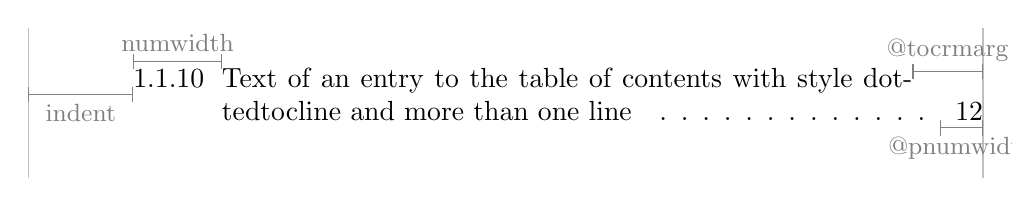
\begin{tikzpicture}
        \draw[color=lightgray] (0,2\baselineskip) -- (0,-2.5\baselineskip);
        \draw[color=lightgray] (\linewidth,2\baselineskip) --
                               (\linewidth,-2.5\baselineskip);
        \node (dottedtocline) at (0,0) [anchor=west,inner sep=0,outer sep=0]
        {%
          \hspace*{7em}%
          \parbox[t]{\dimexpr\linewidth-9.55em}{%
            \setlength{\parindent}{-3.2em}%
            \addtolength{\parfillskip}{-2.55em}%
            \makebox[3.2em][l]{1.1.10}%
            Text of an entry to the table of contents with style
            \PValue{dottedtocline} and more than one line%
            \leaders\hbox{$\csname m@th\endcsname
              \mkern 4.5mu\hbox{.}\mkern 4.5mu$}\hfill\nobreak
            \makebox[1.55em][r]{12}%
          }%
        };
        \draw[|-|,color=gray,overlay] (0,0) --
                              node [anchor=north,font=\small] {
                                \PValue{indent}
                              }
                              (3.8em,0);
        \draw[|-|,color=gray,overlay] (3.8em,\baselineskip) -- 
                              node [anchor=south,font=\small] {
                                \PValue{numwidth}
                              }
                              (7em,\baselineskip);
        \draw[|-|,color=gray,overlay] (\linewidth,\ht\strutbox) -- 
                              node [anchor=south,font=\small] { 
                                \Macro{@tocrmarg} 
                              }
                              (\linewidth-2.55em,\ht\strutbox);
        \draw[|-|,color=gray,overlay] (\linewidth,-\baselineskip) -- 
                              node [anchor=north,font=\small] { 
                                \Macro{@pnumwidth} 
                              } 
                              (\linewidth-1.55em,-\baselineskip);
      \end{tikzpicture}%
    }
    \caption{Illustrations of some attributes of a TOC-entry with style 
      \PValue{dottedtocline}}
    \label{fig:tocbasic.dottedtocline}
  \end{figure}
\item[\PValue{gobble}] is the most ordinary style. Independently from the
  setting of \DescRef{\LabelBase.counter.tocdepth}%
  \IndexCounter{tocdepth}\important{\DescRef{\LabelBase.counter.tocdepth}},
  entries with this style will never be printed.  The style simply gobbles the
  entries. Nevertheless, it supports the standard attribute \PValue{level} but
  does ignore it.
\item[\PValue{largetocline}] is similar to the style used by the standard
  classes for the level \PValue{part}. It supports attributes \PValue{level}
  and \PValue{indent} only. The last one is already a variation of the
  standard classes that do not support an indent of the \PValue{part} entries.

  Before an entry a page break will be made easier. The entries will be
  indented by the value of \PValue{indent} from the left. They are printed
  using \Macro{large}\Macro{bfseries}. If \DescRef{\LabelBase.cmd.numberline}
  is used, the number width is 3\Unit{em}. \DescRef{\LabelBase.cmd.numberline}
  is not redefined. The standard classes do not use
  \DescRef{\LabelBase.cmd.numberline} for \PName{part} entries. The value of
  \PName{indent} even does not influence the indent from the second line of an
  entry.

  \hyperref[fig:tocbasic.largetocline]%
  {Figure~\ref*{fig:tocbasic.largetocline}} illustrates the attributes of this
  style. There you can also see that the style copies inconsistencies of the
  standard classes, e.\,g. the missing indent of the second and following
  lines of an entry or the different values of \Macro{@pnumwidth} that results
  from the font size dependency. This can even result in a to small distance
  between the entry text and the page number. Please note, the entry number
  width shown in the figure is only valid if
  \DescRef{\LabelBase.cmd.numberline} has been used. In contrast, the standard
  classes use a distance of 1\Unit{em} after the number.
  \begin{figure}
    \centering
    \resizebox{.8\linewidth}{!}{%
      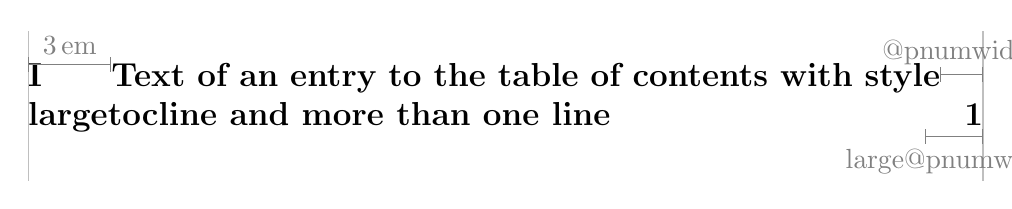
\begin{tikzpicture}
        \draw[color=lightgray] (0,2\baselineskip) -- (0,-2.5\baselineskip);
        \draw[color=lightgray] (\linewidth,2\baselineskip) --
                               (\linewidth,-2.5\baselineskip);
        \node (largetocline) at (0,0) [anchor=west,inner sep=0,outer sep=0] {%
          \parbox[t]{\dimexpr \linewidth-1.55em\relax}{%
            \makebox[3em][l]{\large\bfseries I}%
            \large\bfseries
            Text of an entry to the table of contents with style
            \PValue{largetocline} and more than one line%
            \hfill
            \makebox[0pt][l]{\normalsize\normalfont
              \makebox[1.55em][r]{\large\bfseries 1}}%
          }%
        };
        \draw[|-|,color=gray] (0,\baselineskip) -- 
                              node [anchor=south] { 3\,em } 
                              (3em,\baselineskip);
        \draw[|-|,color=gray,overlay] (\linewidth,\ht\strutbox) -- 
                              node [anchor=south] { \Macro{@pnumwidth} }
                              (\linewidth-1.55em,\ht\strutbox);
        \large\bfseries
        \draw[|-|,color=gray,overlay] (\linewidth,-\baselineskip) -- 
                              node [anchor=north,font=\normalfont\normalsize] { 
                                \Macro{large}\Macro{@pnumwidth} 
                              }
                              (\linewidth-1.55em,-\baselineskip);
      \end{tikzpicture}%
    }
    \caption{Illustrations of some attributes of a TOC-entry with style 
      \PValue{largetocline}}
    \label{fig:tocbasic.largetocline}
  \end{figure}
\item[\PValue{tocline}] is a very flexible style. The \KOMAScript{} classes
  use this style by default for all kinds of entries. Classes \Class{scrbook}
  and \Class{scrreprt} respectively \Class{scrartcl} also define
  clones \PValue{part}, \PValue{chapter} and \PValue{section} respectively
  \PValue{section} and \PValue{subsection}, but add extra
  \PName{initial code} to the clones to change their defaults.

  The style supports attributes \PValue{level}, \PValue{beforeskip},
  \PValue{dynnumwidth}, \PValue{entryformat}, \PValue{entrynumberformat},
  \PValue{breakafternumber}, \PValue{indent}, \PValue{linefill},
  \PValue{numsep}, \PValue{numwidth}, \PValue{onstarthigherlevel},
  \PValue{onstartlowerlevel}, \PValue{onstartsamelevel},
  \PValue{pagenumberbox}, \PValue{pagenumberformat}, \PValue{raggedentrytext},
  and \PValue{raggedpagenumber}. The defaults of all these attributes depend
  on the name of the \PName{entry level}. They correspond to the results of
  the standard classes. So after loading \Package{tocbasic}, you can change
  the style of the standard classes entries to the table of contents into
  \PValue{tocline} using \DescRef{\LabelBase.cmd.DeclareTOCEntryStyle} without obvious visual
  changes unless you change exactly these attributes that should induce such
  changes. Same is valid for list of figures or list of tables of the standard
  classes.

  Because of the flexibility of this style it even could be used instead of
  the styles \PValue{dottedtocline}, \PValue{undottedtocline} or
  \PValue{largetocline}. However it needs more effort for configuration.

  {Figure~\ref*{fig:tocbasic.tocline}} illustrates some of the length
  attributes of this style. All attributes are described in
  \autoref{tab:tocbasic.tocstyle.attributes} from
  \autopageref{tab:tocbasic.tocstyle.attributes}.
  \begin{figure}
    \centering
    \resizebox{.8\linewidth}{!}{%
      \begin{tikzpicture}
        \coordinate (subsection) at (0,0);
        \coordinate (section) at ($(subsection)+(0,2\baselineskip)$);
        \coordinate (chapter) at ($(section)+(0,2\baselineskip)$);
        \coordinate (part)    at ($(chapter)+(0,2.4\baselineskip+1em)$);

        \draw[color=lightgray] 
          ($(part)+(0,2\baselineskip)$) -- 
          (0,-2.5\baselineskip);
        \draw[color=lightgray] 
          ($(part)+(\linewidth,2\baselineskip)$) --
          (\linewidth,-2.5\baselineskip);

        \coordinate (subsection) at (0,0);

        \node at (part) [anchor=west,inner sep=0,outer sep=0]
        {%
          \hspace*{3em}%
          \parbox[t]{\dimexpr\linewidth-5.55em}{%
            \setlength{\parindent}{-3em}%
            \addtolength{\parfillskip}{-2.55em}%
            \makebox[3em][l]{\large\bfseries I.}%
            \textbf{\large Text of a part entry with style
            \PValue{tocline} and with at least two lines of text}%
            \hfill
            \makebox[1.55em][r]{\bfseries 12}\large
          }%
        };
        \draw[|-|,color=gray,overlay] 
          (part) --
          ($(part)+(3em,0)$)
          node [anchor=north east,font=\small] {
            \PValue{numwidth}
          };
        \draw[|-|,color=gray,overlay] 
          ($(part)+(\linewidth,\ht\strutbox)$)
          node [anchor=north,font=\small] { 
            \Macro{@tocrmarg} 
          } --
          ($(part)+(\linewidth-2.55em,\ht\strutbox)$);
        \draw[|-|,color=gray,overlay] 
          ($(part)+(\linewidth,-\baselineskip)$) -- 
          node [anchor=north,font=\small] { 
            \Macro{@pnumwidth} 
          } 
          ($(part)+(\linewidth-1.55em,-\baselineskip)$);
        \node at (chapter) [anchor=west,inner sep=0,outer sep=0]
        {%
          \hspace*{1.5em}%
          \parbox[t]{\dimexpr\linewidth-4.05em}{%
            \setlength{\parindent}{-1.5em}%
            \addtolength{\parfillskip}{-2.55em}%
            \makebox[1.5em][l]{\bfseries 1.}%
            \textbf{Text of a chapter entry with style
            \PValue{tocline} and for demonstration purpose with more than one
            line of text}%
            \hfill
            \makebox[1.55em][r]{\bfseries 12}%
          }%
        };
        \draw[|-|,color=gray,overlay]
          ($(chapter)+(3em,\baselineskip)$) --
          node [anchor=west,font=\small] {
            \PValue{beforeskip}
          }
          ($(part)+(3em,-\baselineskip)$);
        \draw[|-|,color=gray,overlay] 
          (chapter) --
          ($(chapter)+(1.5em,0)$)
          node [anchor=north east,font=\small] {
            \PValue{numwidth}
          };
        \draw[|-|,color=gray,overlay] 
          ($(chapter)+(\linewidth,\ht\strutbox)$)
          node [anchor=north,font=\small] { 
            \Macro{@tocrmarg} 
          } --
          ($(chapter)+(\linewidth-2.55em,\ht\strutbox)$);
        \draw[|-|,color=gray,overlay] 
          ($(chapter)+(\linewidth,-\baselineskip)$)
          node [anchor=north,font=\small] { 
            \Macro{@pnumwidth} 
          } --
          ($(chapter)+(\linewidth-1.55em,-\baselineskip)$);
        \node at (section) [anchor=west,inner sep=0,outer sep=0]
        {
          \hspace*{3.8em}%
          \parbox[t]{\dimexpr\linewidth-6.35em}{%
            \setlength{\parindent}{-2.3em}%
            \addtolength{\parfillskip}{-2.55em}%
            \makebox[2.3em][l]{1.1.}%
            Text of a section entry with style
            \PValue{tocline} and for demonstration purpose with more than one
            line of text%
            \leaders\hbox{$\csname m@th\endcsname
              \mkern 4.5mu\hbox{.}\mkern 4.5mu$}\hfill\nobreak
            \makebox[1.55em][r]{3}%
          }%
        };
        \node at (subsection) [anchor=west,inner sep=0,outer sep=0]
        {%
          \hspace*{7em}%
          \parbox[t]{\dimexpr\linewidth-9.55em}{%
            \setlength{\parindent}{-3.2em}%
            \addtolength{\parfillskip}{-2.55em}%
            \makebox[3.2em][l]{1.1.10.}%
            Text of a subsection entry with style
            \PValue{tocline} and for demonstration purpose with more than one
            line of text%
            \leaders\hbox{$\csname m@th\endcsname
              \mkern 4.5mu\hbox{.}\mkern 4.5mu$}\hfill\nobreak
            \makebox[1.55em][r]{12}%
          }%
        };
        \draw[|-|,color=gray,overlay] 
          ($(subsection)+(0,\ht\strutbox)$) -- 
          node [anchor=north,font=\small] {
            \PValue{indent}
          }
          ($(subsection)+(3.8em,\ht\strutbox)$);
        \draw[|-|,color=gray,overlay] 
          ($(subsection)+(3.8em,0)$) --
          ($(subsection)+(7em,0)$)
          node [anchor=north east,font=\small] {
            \PValue{numwidth}
          };
        \draw[|-|,color=gray,overlay] 
          ($(subsection)+(\linewidth,\ht\strutbox)$)
          node [anchor=north,font=\small] { 
            \Macro{@tocrmarg} 
          } --
          ($(subsection)+(\linewidth-2.55em,\ht\strutbox)$);
        \draw[|-|,color=gray,overlay] 
          ($(subsection)+(\linewidth,-\baselineskip)$) -- 
          node [anchor=north,font=\small] { 
            \Macro{@pnumwidth} 
          } 
          ($(subsection)+(\linewidth-1.55em,-\baselineskip)$);
      \end{tikzpicture}%
    }
    \caption{Illustrations of some attributes of a TOC-entry with style 
      \PValue{tocline}}
    \label{fig:tocbasic.tocline}
  \end{figure}
\item[\PValue{undottedtocline}] is similar to the style used by the standard
  classes \Class{book} and \Class{report} for the \PValue{chapter} entry level
  or by \Class{article} for the \PValue{section} entry level of the table of
  contents. It supports the attributes \PValue{level}, \PValue{indent}, and
  \PValue{numwidth}. The last one is already a variation of the standard
  classes that do not support an indent of these entry levels.

  Before an entry, a page break will be made easier. The entries will be
  indented by the value of \PValue{indent} from the left. They are printed
  using \Macro{bfseries}. \DescRef{\LabelBase.cmd.numberline} is used
  unchanged. The width of the entry number is given by the value of
  \PValue{numwidth}. For multiline entries the indent will be increased by the
  value of \PValue{numwidth} for the second and following
  lines. \hyperref[fig:tocbasic.undottedtocline]%
  {Figure~\ref*{fig:tocbasic.undottedtocline}} illustrates the attributes of
  this style.
  \begin{figure}
    \centering
    \resizebox{.8\linewidth}{!}{%
      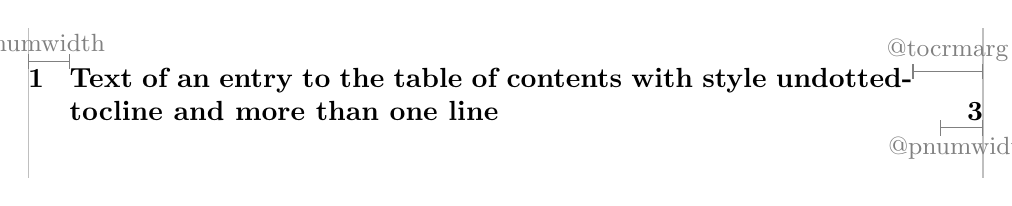
\begin{tikzpicture}
        \draw[color=lightgray] (0,2\baselineskip) -- (0,-2.5\baselineskip);
        \draw[color=lightgray] (\linewidth,2\baselineskip) --
                               (\linewidth,-2.5\baselineskip);
        \node (undottedtocline) at (0,0) [anchor=west,inner sep=0,outer sep=0]
        {%
          \makebox[1.5em][l]{\bfseries 1}%
          \parbox[t]{\dimexpr \linewidth-4.05em\relax}{%
            \bfseries
            Text of an entry to the table of contents with style
            \PValue{undottedtocline} and more than one line%
          }%
          \raisebox{-\baselineskip}{\makebox[2.55em][r]{\bfseries 3}}%
        };
        \draw[|-|,color=gray,overlay] (0,\baselineskip) -- 
                              node [anchor=south,font=\small] {
                                \PValue{numwidth}
                              }
                              (1.5em,\baselineskip);
        \draw[|-|,color=gray,overlay] (\linewidth,\ht\strutbox) -- 
                              node [anchor=south,font=\small] { 
                                \Macro{@tocrmarg} 
                              }
                              (\linewidth-2.55em,\ht\strutbox);
        \draw[|-|,color=gray,overlay] (\linewidth,-\baselineskip) -- 
                              node [anchor=north,font=\small] { 
                                \Macro{@pnumwidth} 
                              } 
                              (\linewidth-1.55em,-\baselineskip);
      \end{tikzpicture}%
    }
    \caption{Illustration of some attributes of style \PValue{undottedtocline}
      by the example of a chapter title}%
    \label{fig:tocbasic.undottedtocline}
  \end{figure}
\end{description}
\hyperref[tab:tocbasic.tocstyle.attributes]%
{Table~\ref*{tab:tocbasic.tocstyle.attributes}} describes all attributes of
all styles defined by
\Package{tocbasic}. If\ChangedAt[2016/06]{v3.21}{\Package{tocbasic}} you want
to use these attributes as options to \DescRef{\LabelBase.cmd.DeclareNewTOC}
(see \DescPageRef{\LabelBase.cmd.DeclareNewTOC}) you have to prefix the names
of the attribute by \PValue{tocentry}, e\,g., attribute \PValue{level} becomes
option \Option{tocentrylevel}.
If\ChangedAt[2015/12]{v3.20}{\Package{tocbasic}} you want to use these
attributes as options to \DescRef{maincls-experts.cmd.DeclareSectionCommand}
(see \DescPageRef{maincls-experts.cmd.DeclareSectionCommand}) and similar
commands you have to prefix the names of the attributes by \PValue{toc},
e\,g., attribute \PValue{level} becomes option \Option{toclevel}.

Last but not least using \Macro{DeclareTOCStyleEntry} will define internal
command \Macro{l@\PName{entry level}}.

\begin{desclist}
  \desccaption{%
    Attributes of the predefined TOC-entry styles of \Package{tocbasic}%
    \label{tab:tocbasic.tocstyle.attributes}%
  }{%
    Attributes of the TOC-entry styles (\emph{continuation})%
  }%
  \entry{\OptionVName{beforeskip}{length}}{%
    vertical distance, inserted before an entry of this level using style
    \PValue{tocline} (see \autoref{fig:tocbasic.tocline}). The distance is
    made using either \Macro{vskip} or \Macro{addvspace} depending on the
    \PName{entry level} to adapt the differences of the standard classes and
    former versions of \KOMAScript.

    At \PName{entry level} \PValue{part} the attribute will be initialised
    with \texttt{2.25em plus 1pt}, at \PValue{chapter} with \texttt{1em plus
      1pt}. If \PName{entry level} currently is unknown, rather
    \PValue{section} is initialised with \texttt{1em plus 1pt}. The initial
    value for all other levels is \texttt{0pt plus .2pt}.%
  }%
  \entry{\OptionVName{breakafternumber}{switch}}{%
    \PName{switch} is one of the values for simple switches from
    \autoref{tab:truefalseswitch}, \autopageref{tab:truefalseswitch}. If the
    switch is active with style \PValue{tocline}, there will be a line break
    after the entry number of
    \DescRef{\LabelBase.cmd.numberline}\IndexCmd{numberline}. The line after
    the entry number again starts left aligned with the number.

    This switch is not active by default at style \PValue{tocline}.

    If\textnote{Attention!} the feature \Option{numberline} of a list of
    something has been activated (see \DescRef{\LabelBase.cmd.setuptoc},
    \autoref{sec:tocbasic.toc}, \DescPageRef{\LabelBase.cmd.setuptoc}), i.\,e.,
    if a \KOMAScript{} class with option
    \OptionValueRef{maincls}{toc}{numberline}%
    \IndexOption{toc~=\PValue{numberline}} is used, then the not numbered
    entries will nevertheless have a (by default empty) number line using the
    format code of \Option{entrynumberformat}.%
  }%
  \entry{\OptionVName{dynnumwidth}{switch}}{%
    \PName{switch} is one of the values for simple switches from
    \autoref{tab:truefalseswitch}, \autopageref{tab:truefalseswitch}. If the
    switch is active with style \PValue{tocline}, attribute \PValue{numwidth}
    is ignored. Instead of that the maximum number width detected at the
    previous \LaTeX{} run increased by the value of \PValue{numsep} is used.%
  }%
  \entry{\OptionVName{entryformat}{command}}{%
    This attributes makes the format of the entry. The value should be a
    \PName{command} with exactly one argument. The \PName{command} should not
    expect the argument to be fully expandable. Commands like
    \Macro{MakeUppercase}, that need a fully expandable argument, must no be
    used here. Font changes are allowed and are relative to
    \Macro{normalfont}\Macro{normalsize}. Please note that the output of
    \Option{linefill} and the page number are independent from
    \Option{entryformat}. See also attribute \Option{pagenumberformat}.

    The initial value of the attribute for \PName{entry level} \PValue{part}
    is printing the argument in \Macro{large}\Macro{bfseries} and for
    \PValue{chapter} printing the argument in \Macro{bfseries}. If currently
    no level \PValue{chapter} exists, \PValue{section} used
    \Macro{bfseries}. All other levels print the argument unchanged.%
  }%
  \entry{\OptionVName{entrynumberformat}{command}}{%
    This attribute makes the format of the entry number within
    \DescRef{\LabelBase.cmd.numberline}. The value should be a \PName{command}
    with exactly one argument. Font changes are relative to the one of
    attribute \Option{entryformat}.

    The initial \PName{command} prints the argument unchanged. This means the
    entry number will be printed as it is.

    If\textnote{Attention!} the feature \Option{numberline} of a list of
    something has been activated (see \DescRef{\LabelBase.cmd.setuptoc},
    \autoref{sec:tocbasic.toc}, \DescPageRef{\LabelBase.cmd.setuptoc}), i.\,e.,
    if a \KOMAScript{} class with option
    \OptionValueRef{maincls}{toc}{numberline}%
    \IndexOption{toc~=\PValue{numberline}}
    is used, then the not numbered entries will nevertheless execute the
    \PName{command}.%
  }%
  \entry{\OptionVName{indent}{length}}{%
    Horizontal distance of the entry relative to the left margin (siehe
    \autoref{fig:tocbasic.dottedtocline} and \autoref{fig:tocbasic.tocline}).

    At style \PValue{tocline} all entry levels with a name that starts with
    ``\texttt{sub}'' are initialised with the sum of the values of
    \PValue{indent} and \PValue{numwidth} of the entry level without this
    prefix. At styles \PValue{dottedtocline}, \PValue{undottedtocline} and
    \PValue{tocline} the initial values of levels \PValue{part} down to
    \PValue{subparagraph} and the levels \PValue{figure} and \PValue{table}
    are compatible with the standard classes. All other levels do not have an
    initial value. Therefore you have to set an explicit value for such levels
    when they are defined first time.%
  }%
  \entry{\OptionVName{level}{integer}}{%
    The numerical value of the \PName{entry level}. Only those entries are
    printed that have a numerical value less or equal to counter
    \DescRef{\LabelBase.counter.tocdepth}%
    \important{\DescRef{\LabelBase.counter.tocdepth}}\IndexCounter{tocdepth}.

    This attribute is mandatory for all styles and will be defined
    automatically at the declaration of the style.

    At style \PValue{tocline} all entry levels with a name starting with
    ``\texttt{sub}'', the initial value is the level value of the entry level
    without this prefix increased by one. At the styles
    \PValue{dottedtocline}, \PValue{largetocline}, \PValue{tocline}, and
    \PValue{undottedtocline} entry levels \PValue{part} down to
    \PValue{subparagraph}, \PValue{figure}, and \PValue{table} are initialised
    compatible with the standard classes. For all other levels the
    initialisation is done with the value of \Macro{\PName{entry
        level}numdepth} if this is defined.%
  }%
  \entry{\OptionVName{linefill}{code}}{%
    At style \PValue{tocline} there can be a filler between the end of the
    entry text and the page number. The value of attribute \PName{linefill} is
    a \PName{code} that prints this filler. For \PName{entry level}
    \PValue{part} and \PValue{chapter} the attribute is initialised with
    \Macro{hfill}. If currently no \PName{entry level} \PValue{chapter} has
    been defined, \PValue{section} also uses \Macro{hfill}. All other entry
    levels are initialised with \DescRef{\LabelBase.cmd.TOCLineLeaderFill} (see
    \DescPageRef{\LabelBase.cmd.TOCLineLeaderFill}).

    If \PName{code} does not result in filling the distance, you should also
    activate attribute \PValue{raggedpagenumber}, to avoid ``\texttt{underfull
      \Macro{hbox}}'' messages.%
  }%
  \entry{\OptionVName{numsep}{length}}{%
    Style \PValue{tocline} tries to ensure a minimum distance of
    \PName{length} between the entry number and the entry text. If
    \PValue{dynnumwidth} is active, it will correct the number width to achieve
    this. Otherwise it simply throws a warning, if the condition is missed.

    The initial \PName{length} is 0.4\Unit{em}.%
  }%
  \entry{\OptionVName{numwidth}{length}}{%
    The reserved width for the entry number (see
    \autoref{fig:tocbasic.dottedtocline} until
    \autoref{fig:tocbasic.undottedtocline}). At the styles
    \PValue{dottedtocline}, \PValue{tocline}, and \PValue{undottedtocline}
    this \PName{length} will be added to the \PName{length} of attribute
    \PValue{indent} for the second and each following entry text line.

    At style \PValue{tocline} the initial \PName{length} of all entries with
    a name starting with ``\texttt{sub}'' is the value of the level without
    this prefix plus 0.9\Unit{em}. At the styles \PValue{dottedtocline},
    \PValue{undottedtocline} and \PValue{tocline} the initial \PName{length}
    of levels \PValue{part} down to \PValue{subparagraph} and levels
    \PName{figure} and \PName{table} is compatible to the standard
    classes. All other levels do not have an initial value. Therefore you
    have to explicitly set \PValue{numwidth} at the first definition of the
    entry.%
  }%
  \entry{\OptionVName{onstarthigherlevel}{code}}{%
    Style \PValue{tocline} can execute \PName{code} at the start of an entry,
    if the numerical level is greater than the numerical level of the previous
    entry. Remember: The numerical level of, e.\,g., \PValue{section} is
    greater than the numerical level of \PValue{part}. Nevertheless
    \PValue{part} has the highest position in the entry hierarchy.

    Please note that the detection of the level of the previous entry depends
    on a valid unchanged value of \Macro{lastpenalty}.

    The initial \PName{code} is \DescRef{\LabelBase.cmd.LastTOCLevelWasLower} (see
    \DescPageRef{\LabelBase.cmd.LastTOCLevelWasLower}).%
  }%
  \entry{\OptionVName{onstartlowerlevel}{code}}{%
    Style \PValue{tocline} can execute \PName{code} at the start of an entry,
    if the numerical level is lower than the numerical level of the previous
    entry. Remember: The numerical level of, e.\,g., \PValue{part} is
    lower than the numerical level of \PValue{section}. Nevertheless
    \PValue{part} has the highest position in the entry hierarchy.

    Please note that the detection of the level of the previous entry depends
    on a valid unchanged value of \Macro{lastpenalty}.

    The initial \PName{code} is \DescRef{\LabelBase.cmd.LastTOCLevelWasHigher} (see
    \DescPageRef{\LabelBase.cmd.LastTOCLevelWasHigher}).%
  }%
  \entry{\OptionVName{onstartsamelevel}{code}}{%
    Style \PValue{tocline} can execute \PName{code} at the start of an entry,
    if the level is same like the level of the previous entry.

    Please note that the detection of the level of the previous entry depends
    on a valid unchanged value of \Macro{lastpenalty}.

    The initial \PName{code} is \DescRef{\LabelBase.cmd.LastTOCLevelWasSame} (see
    \DescPageRef{\LabelBase.cmd.LastTOCLevelWasSame}).%
  }%
  \entry{\OptionVName{pagenumberbox}{command}}{%
    By default the page number of an entry is printed right aligned in a box
    of width \Macro{@pnumwidth}. At style \PValue{tocline} the \PName{command}
    to print the number can be changed using this attribute. The
    \PName{command} should have exactly one argument, the page number.%
  }%
  \entry{\OptionVName{pagenumberformat}{command}}{%
    This attribute is the format of the page number of an entry. The
    \PName{command} should have exactly one argument, the page number. Font
    changes are relative to the font of \Option{entryformat} followed by
    \Macro{normalfont}\Macro{normalsize}.

    The initial \PName{command} of entry level \PValue{part} prints the
    argument in \Macro{large}\Macro{bfseries}. The initial \PName{command} of
    all other levels prints the argument in
    \Macro{normalfont}\Macro{normalcolor}.%
  }%
  \entry{\OptionVName{raggedentrytext}{switch}}{%
    \ChangedAt{v3.21}{\Package{tocbasic}}%
     \PName{switch} is one of the values for simple switches from
    \autoref{tab:truefalseswitch}, \autopageref{tab:truefalseswitch}. If the
    switch is active, style \PValue{tocline} does print the text of an entry
    left-aligned instead of justified and only word, that are longer than a
    text line, are automatically hyphenated.

    This switch is not active by default.%
  }%
 \entry{\OptionVName{raggedpagenumber}{switch}}{%
    \PName{switch} is one of the values for simple switches from
    \autoref{tab:truefalseswitch}, \autopageref{tab:truefalseswitch}. If the
    switch is active, style \PValue{tocline} does not force the page number to
    be right aligned.

    Depending on the value of \PValue{linefill}, the setting of this attribute
    could be needed for the wanted printing of the number, or only to avoid
    unwanted warning messages. So both attributes should correspond.

    By default the switch is not activated and therefore corresponds with an
    initial value \Macro{hfill} or \DescRef{\LabelBase.cmd.TOCLineLeaderFill} of attribute
    \PValue{linefill}.%
  }%
\end{desclist}%
%
\EndIndexGroup


\begin{Declaration}
  \Macro{DeclareTOCEntryStyle}\Parameter{style}%
                              \OParameter{initial code}%
                              \Parameter{command code}%
  \Macro{DefineTOCEntryOption}\Parameter{option}\OParameter{default value}%
                              \Parameter{code}%
  \Macro{DefineTOCEntryBooleanOption}\Parameter{option}%
                                     \OParameter{default value}%
                                     \Parameter{prefix}%
                                     \Parameter{postfix}%
                                     \Parameter{description}%%
                                     %\OParameter{initial code}%
  \Macro{DefineTOCEntryCommandOption}\Parameter{option}%
                                     \OParameter{default value}%
                                     \Parameter{prefix}%
                                     \Parameter{postfix}%
                                     \Parameter{description}%%
                                     %\OParameter{initial code}%
  \Macro{DefineTOCEntryIfOption}\Parameter{option}%
                                     \OParameter{default value}%
                                     \Parameter{prefix}%
                                     \Parameter{postfix}%
                                     \Parameter{description}%%
                                     %\OParameter{initial code}%
  \Macro{DefineTOCEntryLengthOption}\Parameter{option}%
                                     \OParameter{default value}%
                                     \Parameter{prefix}%
                                     \Parameter{postfix}%
                                     \Parameter{description}%%
                                     %\OParameter{initial code}%
  \Macro{DefineTOCEntryNumberOption}\Parameter{option}%
                                     \OParameter{default value}%
                                     \Parameter{prefix}%
                                     \Parameter{postfix}%
                                     \Parameter{description}%
                                     %\OParameter{initial code}%
\end{Declaration}
\Macro{DeclareTOCEntryStyle}\ChangedAt[2016/03]{v3.20}{\Package{tocbasic}} is
one of the most complex commands in \KOMAScript. It is addressed to \LaTeX{}
developers not the \LaTeX{} users. It provides the definition of a new
TOC-entry \PName{style}. Usually TOC-entries are made using
\Macro{addcontentsline}\IndexCmd{addcontentsline}, or, if you use
\Package{tocbasic}, with recommended
\DescRef{\LabelBase.cmd.addxcontentsline}\IndexCmd{addxcontentsline} (see
\autoref{sec:tocbasic.basics},
\DescPageRef{\LabelBase.cmd.addxcontentsline}). In both cases \LaTeX{}
writes a corresponding \Macro{contentsline}\IndexCmd{contentsline} into the
given auxiliary file. Reading this auxiliary file each \Macro{contentsline}
results in execution of a command \Macro{l@\PName{entry level}}.

Whenever you assign a \PName{style} to a TOC-entry level using
\DescRef{\LabelBase.cmd.DeclareTOCStyleEntry}, first of all the \PName{initial
  code} is executed and then \Macro{l@\PName{entry level}} is defined to be
\PName{command code}. So \PName{command code} is the code that will be
expanded and executed by \Macro{l@\PName{entry level}}. Inside \PName{command
  code} \texttt{\#1} is the name of the TOC-entry level and \texttt{\#\#1} and
\texttt{\#\#2} are the arguments of \Macro{l@\PName{entry level}}.

The \PName{initial code} should initialise all attributes of the
\PName{style}. Developers are recommended to use \PName{initial code} to
initialise all internal macros of the \PName{style} without the need of
using an \PName{option list}. The second task of the \PName{initial code} is
the definition of options to setup the attributes of the \PName{style}. Option
\Option{level} is always defined automatically. The value of \Option{level}
can be got in \PName{command code} using
\Macro{@nameuse}\PParameter{\#1tocdepth}%
\important{\Macro{\PName{entry level}tocdepth}}, e.\,g., to compare it with
the counter \DescRef{\LabelBase.counter.tocdepth}\IndexCounter{tocdepth}.

Commands \Macro{DefineTOCEntryBooleanOption},
\Macro{DefineTOCEntryCommandOption}, \Macro{DefineTOCEntryIfOption},
\Macro{DefineTOCEntryLengthOption}, and \Macro{DefineTOCEntryNumberOption}
should be used to define options for the attributes of the
\PName{style} inside \PName{initial code} only. If you use an \PName{option}
defined by one of these commands, a macro \Macro{\PName{prefix}\PName{entry
    level}\PName{postfix}} will be defined to be the assigned value or the
\PName{default value} of the option. Somehow special is
\Macro{DefineTOCEntryIfOption}. It defines \Macro{\PName{prefix}\PName{entry
    level}\PName{postfix}} as a command with two arguments. If the value to
the option is an activation value of \autoref{tab:truefalseswitch},
\autopageref{tab:truefalseswitch} the command expands to the first
argument. If the value to the option is a deactivation value, the command
expands to the second argument.

The \PName{description} should be a real short text that describes the sense
of the option with some catchwords. Package \Package{tocbasic} uses this text
in error messages, warnings or information output on the terminal and into the
\File{log}-file.

The most simple style of \Package{tocbasic}, \PValue{gobble}, is defined
using:
\begin{lstcode}
  \DeclareTOCEntryStyle{gobble}{}%
\end{lstcode}
If you would define a entry level \PValue{dummy} using:
\begin{lstcode}
  \DeclareTOCStyleEntry[level=1]{gobble}{dummy}
\end{lstcode}
among others this would do something like:
\begin{lstcode}
  \def\dummytocdepth{1}
  \def\l@dummy#1#2{}
\end{lstcode}

Inside style \PValue{tocline} for example
\begin{lstcode}
  \DefineTOCEntryCommandOption{linefill}[\TOCLineLeaderFill]%
  {scr@tso@}{@linefill}{filling between text and page number}%
\end{lstcode}
is used to define option \Option{linefill} with \PName{default value}
\DescRef{\LabelBase.cmd.TOCLineLeaderFill}. A call like:
\begin{lstcode}
  \RedeclareTOCStyleEntry[linefill]{tocline}{part}
\end{lstcode}
would therefore result in a definition like:
\begin{lstcode}
  \def\scr@tso@part@linefill{\TOCLineLeaderFill}
\end{lstcode}

Whoever likes to define his own styles is recommended to first study the
definition of style \PValue{dottedtocline}. If this definition is understood,
the much more complex definition of style \PValue{tocline} gives a lot of
hints of the correct usage of the described commands.

In many cases it will be enough to clone an existing style using
\DescRef{\LabelBase.cmd.CloneTOCEntryStyle} and to change the initial code of
the new style using \DescRef{\LabelBase.cmd.TOCEntryStyleInitCode} or
\DescRef{\LabelBase.cmd.TOCEntryStyleStartInitCode}.

\Macro{DefineTOCEntryOption} is merely used to define the other
commands. It is not recommended to define options directly using
\Macro{DefineTOCEntryOption}. Normally this is even not needed. It is
alluded only for completeness.%
\EndIndexGroup


\begin{Declaration}
  \Macro{CloneTOCEntryStyle}\Parameter{style}\Parameter{new style}%
\end{Declaration}
With\ChangedAt[2016/03]{v3.20}{\Package{tocbasic}} this command you can clone
an existing \PName{style}. This defines a \PName{new style} with the same
attributes and settings like the existing \PName{style}. The package itself
uses \Macro{CloneTOCEntryStyle} to declare style \PValue{default} as a clone
of \PValue{dottedtocline}. The \KOMAScript{} classes use the command to
declare the styles \PValue{part}, \PValue{section}, and \PValue{chapter} or
\PValue{subsection} as a clone of \PValue{tocline} and the style
\PValue{default} new as a clone of \PValue{section} or \PValue{subsection}.%
\EndIndexGroup


\begin{Declaration}
  \Macro{TOCEntryStyleInitCode}\Parameter{style}%
                               \Parameter{initial code}%
  \Macro{TOCEntryStyleStartInitCode}\Parameter{style}%
                                    \Parameter{initial code}
\end{Declaration}
Every\ChangedAt[2016/03]{v3.20}{\Package{tocbasic}} TOC-entry style has an
initialisation code. This is used whenever a \PName{style} is assigned to an
TOC-entry using \DescRef{\LabelBase.cmd.DeclareTOCEntryStyle}. This
\PName{initial code} should never do anything global, because it is also used
for local initialisation inside other commands like
\DescRef{\LabelBase.cmd.DeclareNewTOC}\IndexCmd{DeclareNewTOC}. The \PName{initial code} not
only defines all attributes of a \PName{style}. It also should set the
defaults for those attributes.

You can use \Macro{TOCEntryStyleStartInitCode} and
\Macro{TOCEntryStyleInitCode} to extend the already existing initialisation
code by \PName{initial code}. \Macro{TOCEntryStyleStartInitCode} adds
\PName{initial code} in front of the existing initialisation
code. \Macro{TOCEntryStyleInitCode} adds the \PName{initial code} at the end
of the existing initialisation code. The \KOMAScript{} classes, e.\,g., are
using \Macro{TOCEntryStyleStartInitCode} to change the filling, font and
vertical distances of style \PValue{part} that is a clone of
\PValue{tocline}. Class \Class{scrbook} and \Class{scrreprt} use
\begin{lstcode}
  \CloneTOCEntryStyle{tocline}{section}
  \TOCEntryStyleStartInitCode{section}{%
    \expandafter\providecommand%
    \csname scr@tso@#1@linefill\endcsname
    {\TOCLineLeaderFill\relax}%
  }
\end{lstcode}
to declare \PValue{section} as a modified clone of \PValue{tocline}.%
\EndIndexGroup


\begin{Declaration}
  \Macro{LastTOCLevelWasHigher}%
  \Macro{LastTOCLevelWasSame}%
  \Macro{LastTOCLevelWasLower}
\end{Declaration}
At\ChangedAt[2016/03]{v3.20}{\Package{tocbasic}} the very beginning entries
with style \PValue{tocline} \Package{tocbasic} executes one of these three
commands depending on \Macro{lastpenalty}. \Macro{LastTOCLevelWasHigher} and
\Macro{LastTOCLevelWasSame} used in vertical mode add
\Macro{addpenalty}\PParameter{\Macro{@lowpenalty}} and therefore permit a
page break before an entry with same or higher hierarchical
position. \Macro{LastTOCLevelWasLower} is an empty command. Therefore page
break between an entry and its sub-entry is not permitted.

Users should not redefine these commands. Instead of a redefinition you should
change the behaviour of single entry levels using attributes
\PValue{onstartlowerlevel}, \PValue{onstartsamelevel}, and
\PValue{onstarthigherlevel}.%
\EndIndexGroup


\begin{Declaration}
  \Macro{TOCLineLeaderFill}\OParameter{filling code}
\end{Declaration}
Command\ChangedAt[2016/03]{v3.20}{\Package{tocbasic}} has been made to be used
as value of option \Option{linefill} of assigning style \PName{tocline} to a
TOC-entry. It is a line filler between the end of the entry text and the entry
page number. The \PName{filling code} will be repeated with constant
distance. The default for this optional argument is a dot.

As implied by the name of the command it uses \Macro{leaders} to put the
\PName{filling code}. The distance is defined analogous to the \LaTeX{} kernel
command \Macro{@dottedtocline} by
\Macro{mkern}\Macro{@dotsep}\Unit{\texttt{mu}}.%
\EndIndexGroup
\EndIndexGroup


\section{Internal Commands for Class and Package Authors}
\label{sec:tocbasic.internals}

Commands with prefix \Macro{tocbasic@} are internal but class and package
authors may use them. But even if you are a class or package author you
should not change them!

\begin{Declaration}
  \Macro{tocbasic@extend@babel}\Parameter{extension}
\end{Declaration}
The Package \Package{babel}\IndexPackage{babel} (see \cite{package:babel}),
or more specifically a \LaTeX{} kernel that has been extended by the language
management of \Package{babel} writes instructions to change the language
inside of the files with the file name extensions \File{toc}, \File{lof}, and
\File{lot} into those files at every change of the current language either at
the begin of the document or inside the document. Package \Package{tocbasic}
extends this mechanism with \Macro{tocbasic@extend@babel} to be used for other
file name extensions too. Argument \PName{extension} has to be expandable!
Otherwise the meaning of the argument may change until it will be used really.

Normally this command will be used by default for every file name
\PName{extension} that will be added to the list of known extensions using
\DescRef{\LabelBase.cmd.addtotoclist}. This may be suppressed using feature
\PValue{nobabel}\important{\PValue{nobabel}} (see \DescRef{\LabelBase.cmd.setuptoc},
\autoref{sec:tocbasic.toc}, \DescPageRef{\LabelBase.cmd.setuptoc}). For the file
name extensions \File{toc}, \File{lof}, and \File{lot} this will be done
automatically by \Package{tocbasic} to avoid double language switching in the
corresponding files.

Normally there isn't any reason to call this command yourself. But there may
by lists of something, that should not be under control of \Package{tocbasic},
and so are not in \Package{tocbasic}'s list of known file name extensions, but
nevertheless should be handled by the language change mechanism of
\Package{babel}. The command may be used explicitly for those files. But please
note that this should be done only once per file name extension!%
\EndIndexGroup


\begin{Declaration}
  \Macro{tocbasic@starttoc}\Parameter{extension}
\end{Declaration}
This command is something like the \LaTeX{} kernel macro
\Macro{@starttoc}\IndexCmd{@starttoc}\important{\Macro{@starttoc}}.  It is the
command behind \DescRef{\LabelBase.cmd.listoftoc*} (see \autoref{sec:tocbasic.toc},
\DescPageRef{\LabelBase.cmd.listoftoc*}). Authors of classes or packages
who want to participate from the advantages of \Package{tocbasic} should at
least use this command. Nevertheless it is recommended to use
\DescRef{\LabelBase.cmd.listoftoc}. Command \Macro{tocbasic@starttoc} internally uses
\Macro{\@starttoc}, but sets
\Length{parskip}\IndexLength{parskip}\important{\Length{parskip}\\
  \Length{parindent}\\
  \Length{parfillskip}} and \Length {parindent}\IndexLength{parindent} to 0
and \Length{parfillskip} to 0 until infinite before. Moreover,
\Macro{@currext}\important{\Macro{@currext}}\IndexCmd{@currext} will be set to
the file name extension of the current TOC-file, so this will be available
while the execution of the hooks, that will be done before and after reading
the auxiliary files.

Because\textnote{Attention!} of \LaTeX{} will immediately open a new TOC-file
for writing after reading that file, the usage of \Macro{tocbasic@starttoc}
may result in an error message like
\begin{lstoutput}
  ! No room for a new \write .
  \ch@ck ...\else \errmessage {No room for a new #3}
                                                    \fi
\end{lstoutput}
if there are no more unused write handles. This may be solved, e.\,g., using
package
\Package{scrwfile}\important{\Package{scrwfile}}\IndexPackage{scrwfile}.
See \autoref{cha:scrwfile} for more information about that package.%
\EndIndexGroup


\begin{Declaration}
  \Macro{tocbasic@@before@hook}%
  \Macro{tocbasic@@after@hook}
\end{Declaration}
The hook \Macro{tocbasic@@before@hook} will be executed immediately before
reading a auxiliary file for a TOC even before execution of the instructions
of a \DescRef{\LabelBase.cmd.BeforeStartingTOC} command. It is permitted to
extend this hook using \Macro{g@addto@macro}\IndexCmd{g@addto@macro}.

Similarly \Macro{tocbasic@@after@hook} will be executed immediately after
reading such an auxiliary file and before execution of instructions of
\DescRef{\LabelBase.cmd.AfterStartingTOC}. It is permitted to extend this hook
using \Macro{g@addto@macro}\IndexCmd{g@addto@macro}.

\KOMAScript{} uses these hooks, to provide the automatic width calculation of
the place needed by heading numbers. Only classes and packages should use
these hooks. Users\textnote{Attention!} should really use
\DescRef{\LabelBase.cmd.BeforeStartingTOC} and
\DescRef{\LabelBase.cmd.AfterStartingTOC} instead. Authors of packages should
also favour those commands! These hooks should not be used to generate any
output!

If neither\textnote{Attention!} \DescRef{\LabelBase.cmd.listofeachtoc} nor
\DescRef{\LabelBase.cmd.listoftoc} nor \DescRef{\LabelBase.cmd.listoftoc*} are
used for the output of a TOC, the hooks should be executed explicitly.%
\EndIndexGroup


\begin{Declaration}
  \Macro{tocbasic@\PName{extension}@before@hook}%
  \Macro{tocbasic@\PName{extension}@after@hook}
\end{Declaration}
These hooks are processed after \DescRef{\LabelBase.cmd.tocbasic@@before@hook}, respectively
before \DescRef{\LabelBase.cmd.tocbasic@@after@hook} before and after loading the TOC-file with
the corresponding file \PName{extension}. Authors\textnote{Attention!}  of
classes and packages should never manipulate them! But if
neither\textnote{Attention!} \DescRef{\LabelBase.cmd.listofeachtoc} nor
\DescRef{\LabelBase.cmd.listoftoc} nor \DescRef{\LabelBase.cmd.listoftoc*} are
used for the output of a TOC, the hooks should be executed explicitly, if they
are defined. Please note that they even can be undefined.%
\EndIndexGroup


\begin{Declaration}
  \Macro{tocbasic@listhead}\Parameter{title}
\end{Declaration}
This command is used by \DescRef{\LabelBase.cmd.listoftoc} to set the heading of the TOC,
either the default heading or the individually defined heading. If you define
your own TOC-command not using \DescRef{\LabelBase.cmd.listoftoc} you may use
\Macro{tocbasic@listhead}. In this case you should define
\Macro{@currext}\important{\Macro{@currext}}\IndexCmd{@currext} to be the file
extension of the corresponding TOC-file before using
\Macro{tocbasic@listhead}.%
\EndIndexGroup


\begin{Declaration}
  \Macro{tocbasic@listhead@\PName{extension}}\Parameter{title}
\end{Declaration}
This command is used in \DescRef{\LabelBase.cmd.tocbasic@listhead} to set the individual
headings, optional table of contents entry, and running head, if it was
defined. If it was not defined it will be defined and used in
\DescRef{\LabelBase.cmd.tocbasic@listhead} automatically.
\EndIndexGroup


\begin{Declaration}
  \Macro{tocbasic@addxcontentsline}%
  \Parameter{extension}\Parameter{level}\Parameter{number}\Parameter{text}%
  \Macro{nonumberline}
\end{Declaration}
Command\ChangedAt{v3.12}{\Package{tocbasic}} \Macro{tocbasic@addxcontentsline}
uses \Macro{addcontentsline} to either create a numbered or not numbered text
entry to the TOC-file with the given \PName{extension}. Note, all parameters
of \Macro{tocbasic@addxcontentsline} are mandatory. But you may use an empty
\PName{number} argument, if you do not want a number. In this case the
\PName{text} will be prefixed by \Macro{nonumberline} without any argument. In
the other case, if \PName{number} is not empty,
\DescRef{\LabelBase.cmd.numberline} with argument \PName{number} will used as
usual.

Command \Macro{nonumberline} is redefined inside
\DescRef{\LabelBase.cmd.listoftoc} (see \autoref{sec:tocbasic.toc},
\DescPageRef{\LabelBase.cmd.listoftoc}) depending on feature \PValue{numberline}
(see \autoref{sec:tocbasic.toc}, \DescPageRef{\LabelBase.cmd.setuptoc}). This
guarantees that changes of the feature results in changes of the corresponding
TOC immediately at the next \LaTeX{} run.%
\EndIndexGroup


\begin{Declaration}
  \Macro{tocbasic@DependOnPenaltyAndTOCLevel}\Parameter{entry level}%
  \Macro{tocbasic@SetPenaltyByTOCLevel}\Parameter{entry level}
\end{Declaration}
At\ChangedAt[2016/03]{v3.20}{\Package{tocbasic}} the end of TOC-entry style
\PValue{tocline} (see \autoref{sec:tocbasic.tocstyle}) \Macro{penalty} is set
to prohibit page breaks. The used penalty value depends on the \PName{entry
  level}. This is done by \Macro{tocbasic@SetPenaltyByTOCLevel}. At the very
beginning of an entry \Macro{tocbasic@DependOnPenaltyAndTOCLevel} is used to
execute the value of either style option \Option{onstartlowerlevel},
\Option{onstartsamelevel}, or \Option{onstarthigherlevel} depending on
\Macro{lastpenalty} and the current \PName{entry level}. The default of the
first and second option would be to permit a page break, if used in vertical
mode.

Developers of \PValue{tocline}-compatible styles should adapt this. To do so,
they are even allowed to copy the style option declarations of
\Option{onstartlowerlevel}, \Option{onstartsamelevel}, and
\Option{onstarthigherlevel}. These options should even use the same internal
macros \Macro{scr@tso@\PName{entry level}@LastTOCLevelWasHigher},
\Macro{scr@tso@\PName{entry level}@LastTOCLevelWasSame} and
\Macro{scr@tso@\PName{entry level}@LastTOCLevelWasLower} to store the current
values of the options.%
\EndIndexGroup


\section{A Complete Example}
\seclabel{example}

This section will show you a complete example of a user defined floating
environment with list of that kind of floats and \KOMAScript{} integration
using \Package{tocbasic}. This example uses internal commands, that have a
``\texttt{@}'' in their name. This means\textnote{Attention}, that the code
has to be put into a package or class, or has to be placed between
\Macro{makeatletter}\important[i]{\Macro{makeatletter}\\\Macro{makeatother}}%
\IndexCmd{makeatletter} and \Macro{makeatother}\IndexCmd{makeatother}.

First\textnote{environment} of all, a new floating environment will be
needed. This could simply be done using:
\begin{lstcode}
  \newenvironment{remarkbox}{%
    \@float{remarkbox}%
  }{%
    \end@float
  }
\end{lstcode}
To the new environment is named \Environment{remarkbox}.

Each\textnote{placement} floating environment has a default
placement. This is build by some of the well known placement options:
\begin{lstcode}
  \newcommand*{\fps@remarkbox}{tbp}
\end{lstcode}
So, the new floating environment should be placed by default only either at
the top of a page, at the bottom of a page, or on a page on its own.

Floating\textnote{type} environments have a numerical floating
type. Environments with the same active bit at the floating type cannot change
their order. Figures and table normally use type~1 and 2. So a figure that
comes later at the source code than a table, may be output earlier than the
table and vica versa.
\begin{lstcode}
  \newcommand*{\ftype@remarkbox}{4}
\end{lstcode}
The new environment has floating type~4, so it may pass figures and floats and
may be passed by those.

The\textnote{number} captions of floating environment also have numbers.
\begin{lstcode}
  \newcounter{remarkbox}
  \newcommand*{\remarkboxformat}{%
    Remark~\theremarkbox\csname autodot\endcsname}
  \newcommand*{\fnum@remarkbox}{\remarkboxformat}
\end{lstcode}
Here first a new counter has been defined, that is independent from chapters
or the counters of other structural levels. \LaTeX{} itself also defines
\Macro{theremarkbox} with the default Arabic representation of the counter's
value. Afterwards this has been used defining the formatted output of the
counter. Last this formatted output has been used for the output of the
environment number of the \DescRef{maincls.cmd.caption} command.

Floating\textnote{file name extension} environments have lists of themselves
and those need a auxiliary file with name \Macro{jobname} and a file name
extension, the TOC-file\Index{TOC-file}:
\begin{lstcode}
  \newcommand*{\ext@remarkbox}{lor}
\end{lstcode}
The file name extension of the TOC-file for the list of
\Environment{remarkbox}es is ``\File{lor}''.

This was the definition of the floating environment. But the list of this new
environment's captions is still missing. To reduce the implementation effort
package \Package{tocbasic} will be used for this. This will be loaded using
\begin{lstcode}
  \usepackage{tocbasic}
\end{lstcode}
inside of document preambles. Authors of classes or packages would use
\begin{lstcode}
  \RequirePackage{tocbasic}
\end{lstcode}
instead.

Now\textnote{extension} we register the file name extension for package
\Package{tocbasic}:
\begin{lstcode}
  \addtotoclist[float]{lor}
\end{lstcode}
Thereby the owner \PValue{float} has been used, to allude all further
\KOMAScript{} options for list of figures and list of tables also to the new
one.

Next\textnote{title} we define a title or heading for the list of
\Environment{remarkbox}es:
\begin{lstcode}
  \newcommand*{\listoflorname}{List of Remarks}
\end{lstcode}
You may use package \Package{scrbase} to additionally support titles in other
languages than English.

Also\textnote{entry} a command is needed to define the layout of the entries
to the list of remarks:
\begin{lstcode}
  \newcommand*{\l@remarkbox}{\l@figure}
\end{lstcode}
Here simply the entries to the list of remarks get the same layout like the
entries to the list of figures. This would be the easiest solution. A more
explicit would be, e.\,g.,
\begin{lstcode}
  \DeclareTOCStyleEntry[level=1,indent=1em,numwidth=1.5em]%
                       {tocline}{remarkbox}
\end{lstcode}

Additionally\textnote{chapter entry} you may want structure the list of
remarks depending on chapters.
\begin{lstcode}
  \setuptoc{lor}{chapteratlist}
\end{lstcode}
The \KOMAScript{} classes provide that feature and maybe other classes do so
too. Unfortunately the standard classes do not.

This\textnote{list of remarks} would already be enough. Now, users may already
select different kinds of headings either using the corresponding options of
the \KOMAScript{} classes, or \DescRef{\LabelBase.cmd.setuptoc}, e.\,g., with
or without entry in the table of contents, with or without number. But a
simple
\begin{lstcode}
  \newcommand*{\listofremarkboxes}{\listoftoc{lor}}
\end{lstcode}
may make the usage a little bit easier again.

As you've seen only five commands refers to the list of remarks. Only three of
them are necessary. Nevertheless the new list of remarks already provides
optional numbering of the heading and optional not numbered entry into the
table of contents. Optional even a lower document structure level may be used
for the heading. Running headers are provides with the \KOMAScript{} classes,
the standard classes, and all classes that explicitly support
\Package{tocbasic}. Supporting classes even pay attention to this new list of
remarks at every new \DescRef{maincls.cmd.chapter}. Even changes of the
current language are handled inside the list of remarks like they will inside
the list of figures or inside the list of tables.

Moreover,\textnote{additional features} an author of a package may add more
features. For example, options to hide \DescRef{\LabelBase.cmd.setuptoc} from
the users may be added. On the other hand, the \Package{tocbasic} manual may
be referenced to describe the corresponding features. The advantage of this
would be that user would get information about new features provides by
\Package{tocbasic}. But if the user should be able to set the features of the
remarks even without knowledge about the file name extension \File{lor} a
simple
\begin{lstcode}
  \newcommand*{\setupremarkboxes}{\setuptoc{lor}}
\end{lstcode}
would be enough to use a list of features argument to
\Macro{setupremarkboxes} as list of features of file name extension \File{lor}.

\section{Everything with One Command Only}
\label{sec:tocbasic.highlevel}

The example from the previous section shows, that using \Package{tocbasic} to
define floating environments and lists with the captions of those floating
environments is easy. The following example will show, that it may be even
easier.

\begin{Declaration}
  \Macro{DeclareNewTOC}\OParameter{options}\Parameter{extension}
\end{Declaration}
This command declares\ChangedAt{v3.06}{\Package{tocbasic}} in one step only a
new TOC, the heading of that TOC, the term used for the TOC-entries, and to
manage the file name \PName{extension}. Additionally optional floating and
non-floating environments may be defined, and inside of both such environments
\DescRef{maincls.cmd.caption}%
\important{\DescRef{maincls.cmd.caption}}\IndexCmd{caption} may be used. The
additional features \DescRef{maincls.cmd.captionabove}\important[i]{%
  \DescRef{maincls.cmd.captionabove}\\
  \DescRef{maincls.cmd.captionbelow}}, \DescRef{maincls.cmd.captionbelow}, and
\DescRef{maincls.env.captionbeside} of the \KOMAScript{} classes (see
\autoref{sec:maincls.floats}) may also be used inside of those environments.

Argument \PName{extension} is the file name extension of the TOC-file, that
represents the list of something. See \autoref{sec:tocbasic.basics} for more
information about this. This argument is mandatory and must not be empty!

Argument \PName{options} is a comma separated list, like you know it from,
e.\,g., \DescRef{maincls.cmd.KOMAoptions} (see
\autoref{sec:typearea.options}). Nevertheless\textnote{Attention!}, those
options cannot be set using
\DescRef{maincls.cmd.KOMAoptions}\IndexCmd{KOMAoptions}! An overview of all
available options may be found in
\autoref{tab:tocbasic.DeclareNewTOC-options}.

If\ChangedAt[2015/12]{v3.20}{\Package{tocbasic}} option \Option{tocentrystyle}
is not used, style \PValue{default} will be used. For information about this
style see \autoref{sec:tocbasic.tocstyle}. If you do not want to define a
command for entries to the list of something, you can use an empty argument,
i.\,e., \OptionValue{tocentrystyle}{} or
\OptionValue{tocentrystyle}{\PParameter{}}. Nevertheless, this would contain
the risk to get a lot of errors while printing that list.

Depending\ChangedAt[2015/12]{v3.20}{\Package{tocbasic}}%
\ChangedAt[2016/06]{v3.21}{\Package{tocbasic}} on the style of the entries to
the list of something, you can setup all valid attributes of the selected
style as part of the \PName{options}. To do so you have to prefix the names of
the attributes given in \autoref{tab:tocbasic.tocstyle.attributes} from
\autopageref{tab:tocbasic.tocstyle.attributes} by prefix
\PValue{tocentry}. Later changes of the style of the entries can be made using
\DescRef{\LabelBase.cmd.DeclareTOCStyleEntry}%
\IndexCmd{DeclareTOCStyleEntry}%
\important{\DescRef{\LabelBase.cmd.DeclareTOCStyleEntry}}. See
\autoref{sec:tocbasic.tocstyle},
\DescPageRef{\LabelBase.cmd.DeclareTOCStyleEntry} for more information about
the styles.%
%
\begin{desclist}
  \renewcommand*{\abovecaptionskipcorrection}{-\normalbaselineskip}%
  \desccaption[{Options for command \Macro{DeclareNewTOC}}]{%
    Options for command
    \Macro{DeclareNewTOC}\ChangedAt{v3.06}{\Package{tocbasic}}%
    \label{tab:tocbasic.DeclareNewTOC-options}%
  }{%
    Options for command \Macro{DeclareNewTOC} (\emph{continuation})%
  }%
  \entry{\OptionVName{atbegin}{instructions}%
    \ChangedAt{v3.09}{\Package{tocbasic}}}{%
    The \PName{instructions} will be executed at the begin of the floating or
    non-floating environment.%
  }%
  \entry{\OptionVName{atend}{instructions}%
    \ChangedAt{v3.09}{\Package{tocbasic}}}{%
    The \PName{instructions} will be executed at the end of the floating or
    non-floating environment.%
  }%
  \entry{\OptionVName{counterwithin}{\LaTeX{} counter}}{%
    If you define a float or non-float, the captions will be numbered and a
    counter \PName{type} (see option \Option{type}) will be defined. You may
    declare another counter to be the parent \LaTeX{} counter. In this case,
    the parent counter will be set before the float counter and the float
    counter will be reset whenever the parent counter is increased using
    \Macro{stepcounter} or \Macro{refstepcounter}.%
  }%
  \entry{\Option{float}}{%
    If set, float environments for that type will be defined. The names of the
    environments are the value of \PName{type} and for double column floats
    the value of \PName{type} with addendum ``\PValue{*}''.%
  }%
  \entry{\OptionVName{floatpos}{float positions}}{%
    The default floating position of the float. If no float position was
    given, ``tbp'' will be used like the standard classes do for figures and
    tables.%
  }%
  \entry{\OptionVName{floattype}{number}}{%
    The numerical float type of the defined floats. Float types with common
    bits cannot be reordered. At the standard classes figures has float type 1
    and tables has float type 2. If no float type was given, 16 will be used.%
  }%
  \entry{\Option{forcenames}}{%
    If set, the names will be even defined, if they where already defined
    before.%
  }%
  \entry{\OptionVName{hang}{length}}{%
    \ChangedAt[2015/12]{v3.20}{\Package{tocbasic}}%
    \ChangedAt[2015/12]{v3.21}{\Package{tocbasic}}%
    This option is deprecated since \KOMAScript~3.20.  Now, the amount of the
    hanging indent of the entries for that list\index{table of contents>entry}
    depend on attributes of the TOC-entry style given by option
    \Option{tocentrystyle}. The styles of \KOMAScript{} provide an attribute
    \PValue{numwidth}. If the used style has such an attribute,
    \Macro{DeclareNewTOC} will initialise it with 1.5\Unit{em}. You can change
    the real \PName{value} using \OptionVName{tocentrynumwidth}{value}. The
    \KOMAScript{} classed for example use
    \OptionValue{tocentrynumwidth}{2.3em}.%
  }%
  \entry{\OptionVName{indent}{length}}{%
    \ChangedAt[2015/12]{v3.20}{\Package{tocbasic}}%
    \ChangedAt[2015/12]{v3.21}{\Package{tocbasic}}%
    This option is deprecated since \KOMAScript~3.20.  Now, the amount of
    indenting the entries of that list\index{table of contents>entry} depend
    on attributes of the TOC-entry style given by option
    \Option{tocentrystyle}. The styles of \KOMAScript{} provide an attribute
    \PValue{indent}.  If the used style has such an attribute,
    \Macro{DeclareNewTOC} will initialise it with 1\Unit{em}. You can change
    the real \PName{value} using \OptionVName{tocentryindent}{value}. The
    \KOMAScript{} classed for example use
    \OptionValue{tocentrynumwidth}{1.5em}.%
  }%
  \entry{\OptionVName{level}{number}}{%
    \ChangedAt[2015/12]{v3.20}{\Package{tocbasic}}%
    \ChangedAt[2015/12]{v3.21}{\Package{tocbasic}}%
    This option is deprecated since \KOMAScript~3.20.  Now, the level of the
    entries of that list\index{table of contents>entry} depend on attributes
    of the TOC-entry style given by option
    \Option{tocentrystyle}. Nevertheless all styles have an attribute
    \PValue{level} and \Macro{DeclareNewTOC} initialises it with 1. You can
    change the real \PName{value} using \OptionVName{tocentrylevel}{value}.%
  }%
  \entry{\OptionVName{listname}{string}}{%
    The name of the TOC. If not given the value of \PValue{types} with upper
    case first char using \Macro{MakeUppercase}\IndexCmd{MakeUppercase}
    prefixed by ``List of '' will be used.%
  }%
  \entry{\OptionVName{name}{string}}{%
    The name of an element. If no name is given, the value of \PValue{type}
    with upper case first char will be used.%
  }%
  \entry{\Option{nonfloat}}{%
    If set, a non floating environment will be defined. The name of the
    environment is the value of \PName{type} with attached ``\PValue{-}''.%
  }%
  \entry{\OptionVName{owner}{string}}{%
    The owner as described in the sections before. If no owner was given owner
    \PValue{float} will be used.%
  }%
  \entry{\OptionVName{tocentrystyle}{TOC-entry style}}{%
    \ChangedAt[2015/12]{v3.20}{\Package{tocbasic}}%
    \PName{TOC-entry style} is the style that should be used for all entries
    into the TOC corresponding to the \PName{extension}. The name of the entry
    level is given by option \Option{type}. Additional to the options of this
    table all attributes of the \PName{TOC-entry style} can be used as
    options. To do so, you have to prefix the name of such an attribute by
    \PValue{toc}. For example, you can change the numerical level of the
    entries using option \Option{tocentrylevel}. For more information about
    the styles and their attributes see \autoref{sec:tocbasic.tocstyle} from
    \autopageref{sec:tocbasic.tocstyle}.%
  }%
  \entry{\OptionVName{tocentry\PName{style-option}}{value}}{%
    \ChangedAt[2015/12]{v3.20}{\Package{tocbasic}}%
    Additional options depending on the \PName{TOC-entry style} given by
    \Option{tocentrystyle}. See \autoref{sec:tocbasic.tocstyle},
    \autopageref{sec:tocbasic.tocstyle} for additional information about
    TOC-entry styles. See \autoref{tab:tocbasic.tocstyle.attributes},
    \autopageref{tab:tocbasic.tocstyle.attributes} for information about the
    attributes of the predefined TOC-entry styles of package
    \Package{tocbasic}, that can be used as \PName{style-option}.%
  }%
  \entry{\OptionVName{type}{string}}{%
    sets the type of the new declared TOC. The type will be used e.\,g. to
    defined a \Macro{listof}\PName{string}. If no type is set up the extension
    from the mandatory argument will be used.%
  }%
  \entry{\OptionVName{types}{string}}{%
    the plural of the type. If no plural was given the value of \PValue{type}
    with attached ``s'' will be used.%
  }%
\end{desclist}

\begin{Example}
  Using \Macro{DeclareNewTOC} reduces the example from
  \autoref{sec:tocbasic.example} to:
\begin{lstcode}
  \DeclareNewTOC[%
    type=remarkbox,%
    types=remarkboxes,%
    float,% define a floating environment
    floattype=4,%
    name=Remark,%
    listname={List of Remarks}%
  ]{lor}
  \setuptoc{lor}{chapteratlist}
\end{lstcode}
  Beside environments \Environment{remarkbox} and \Environment{remarkbox*} the
  counter \Counter{remarkbox}, the commands \Macro{theremarkbox},
  \Macro{remarkboxname}, and \Macro{remarkboxformat} that are used for
  captions; the commands \Macro{listremarkboxnames} and
  \Macro{listofremarkboxes} that are used at the list of remarks; and some
  internal commands that depends on the file name extension \File{lor} are
  defined. If the package should use a default for the floating type, option
  Option{floattype} may be omitted. If option \Option{nonfloat} will be used
  additionally, then a non-floating environment \Environment{remarkbox-} will
  be also defined. You may use \DescRef{maincls.cmd.caption}\IndexCmd{caption} inside of
  that non-floating environment as usual for floating environments.
  \hyperref[tab:tocbasic.comparison]{Figure~\ref*{tab:tocbasic.comparison}}
  shows a comparison of the commands, counters and environments of the
  example environment \Environment{remarkbox} and of the commands, counters
  and environments for figures.%
  \begin{table}
    \centering
    \caption{Comparison of example environment \Environment{remarkbox}
      and environment \Environment{figure}}
    \label{tab:tocbasic.comparison}
    \begin{tabularx}{\textwidth}{ll>{\raggedright}p{6em}X}
      \toprule
      \Environment{remarkbox} & \Environment{figure}
      & options of \Macro{DeclareNewTOC} & short description \\[1ex]
      \midrule
      \Environment{remarkbox} & \Environment{figure}
      & \Option{type}, \Option{float}
      & floating environments of the respective types\\[1ex]
      \Environment{remarkbox*} & \Environment{figure*}
      & \Option{type}, \Option{float}
      & columns spanning floating environments of the respective types\\[1ex]
      \Counter{remarkbox} & \Counter{figure}
      & \Option{type}, \Option{float}
      & counter used by \DescRef{maincls.cmd.caption}\\[1ex]
      \Macro{theremarkbox} & \Macro{thefigure}
      & \Option{type}, \Option{float}
      & output command to the respective counters\\[1ex]
      \Macro{remarkboxformat} & \DescRef{maincls.cmd.figureformat}
      & \Option{type}, \Option{float}
      & formatting command to the respective counters used by
        \DescRef{maincls.cmd.caption}\\[1ex]
      \Macro{remarkboxname} & \Macro{figurename}
      & \Option{type}, \Option{float}, \Option{name}
      & names used in the label of \DescRef{maincls.cmd.caption}\\[1ex]
      \Macro{listofremarkboxes} & \DescRef{maincls.cmd.listoffigures}
      & \Option{types}, \Option{float}
      & command to show the list of the respective environments\\[1ex]
      \Macro{listremarboxname} & \Macro{listfigurename}
      & \Option{type}, \Option{float}, \Option{listname}
      & heading text of the respective list \\[1ex]
      \Macro{fps@remarkbox} & \Macro{fps@figure}
      & \Option{type}, \Option{float}, \Option{floattype}
      & numeric float type for order perpetuation\\[1ex]
      \File{lor} & \File{lof}
      &
      & file name extension of the TOC-file of the respective list \\
      \bottomrule
    \end{tabularx}
  \end{table}

  And now a possible usage of the example environment:
\begin{lstcode}
  \begin{remarkbox}
    \centering
    Equal should be typeset equally
    and with equal formatting.
    \caption{First theorem of typography}
    \label{rem:typo1}
  \end{remarkbox}
\end{lstcode}
  A segment of an example page with this environment could be:
  \begin{center}\footnotesize
    \begin{tabular}
      {|!{\hspace{.1\linewidth}}p{.55\linewidth}!{\hspace{.1\linewidth}}|}
      \\
      \centering
      Equal should be typeset equally
      and with equal formatting.\\[\abovecaptionskip]
      {%
        \usekomafont{caption}\footnotesize{\usekomafont{captionlabel}%
          Remark 1: }First theorem of typography
      }\\
    \end{tabular}%
  \end{center}%
\end{Example}

Users of \Package{hyperref} should always use option
\Option{listname}. Otherwise they may get an error message, because
\Package{hyperref} usually has a problem with the
\Macro{MakeUppercase}\IndexCmd{MakeUppercase} command that is used to change
the case of the first letter of \Option{types} in the name of the list.%
\EndIndexGroup
%
\EndIndexGroup
%
\endinput

%%% Local Variables:
%%% mode: latex
%%% mode: flyspell
%%% coding: us-ascii
%%% ispell-local-dictionary: "en_GB"
%%% TeX-master: "../guide"
%%% End:


%  LocalWords:  Multiline multiline

% ======================================================================
% scrhack.tex
% Copyright (c) Markus Kohm, 2001-2017
%
% This file is part of the LaTeX2e KOMA-Script bundle.
%
% This work may be distributed and/or modified under the conditions of
% the LaTeX Project Public License, version 1.3c of the license.
% The latest version of this license is in
%   http://www.latex-project.org/lppl.txt
% and version 1.3c or later is part of all distributions of LaTeX 
% version 2005/12/01 or later and of this work.
%
% This work has the LPPL maintenance status "author-maintained".
%
% The Current Maintainer and author of this work is Markus Kohm.
%
% This work consists of all files listed in manifest.txt.
% ----------------------------------------------------------------------
% scrhack.tex
% Copyright (c) Markus Kohm, 2001-2017
%
% Dieses Werk darf nach den Bedingungen der LaTeX Project Public Lizenz,
% Version 1.3c, verteilt und/oder veraendert werden.
% Die neuste Version dieser Lizenz ist
%   http://www.latex-project.org/lppl.txt
% und Version 1.3c ist Teil aller Verteilungen von LaTeX
% Version 2005/12/01 oder spaeter und dieses Werks.
%
% Dieses Werk hat den LPPL-Verwaltungs-Status "author-maintained"
% (allein durch den Autor verwaltet).
%
% Der Aktuelle Verwalter und Autor dieses Werkes ist Markus Kohm.
% 
% Dieses Werk besteht aus den in manifest.txt aufgefuehrten Dateien.
% ======================================================================
%
% Chapter about scrhack of the KOMA-Script guide
% Maintained by Markus Kohm
%
% ----------------------------------------------------------------------------
%
% Kapitel ueber scrhack in der KOMA-Script-Anleitung
% Verwaltet von Markus Kohm
%
% ============================================================================

\KOMAProvidesFile{scrhack.tex}
                 [$Date: 2017-03-31 12:00:24 +0200 (Fri, 31 Mar 2017) $
                  KOMA-Script guide (chapter: scrhack)]
\translator{Markus Kohm}

% Date of the translated German file: 2017-01-02
\chapter{Hacks for Third-Party Packages by Package \Package{scrhack}}
\labelbase{scrhack}

\BeginIndexGroup
\BeginIndex{Package}{scrhack}
Some packages from other authors could have problems with \KOMAScript{}.  In my
opinion some packages could be improved. With some packages this makes only
sense, if \KOMAScript{} was used. With some other packages the package author
has another opinion. Sometimes proposals was never answered. Package
\Package{scrhack} contains all those improvement proposals for other
packages. This means, \Package{scrhack} redefines macros of packages from
other authors! The redefinitions are only activated, if those packages were
loaded. Users can prevent \Package{scrhack} from redefining macros of
individual packages.

\section{State of Development Note}
\label{scr:scrhack.draft}

Though this package is part of \KOMAScript{} for long time and though it has
been used by lot of users, there's one problem with it. While redefinition of
macros of foreign packages, it depend on the exact definition an usage of
those macros. This means additionally, that it depends on dedicated releases
of those packages. If a unknown release of such a package will be used,
\Package{scrhack} eventually could not do the needed patch. Contrary, in
extreme cases the patch can cause errors and fault.

So \Package{scrhack} has to be continuously modified to fit new releases of
foreign packages and will never be finished. Because of this \Package{scrhack}
will stay in beta state forever. Though the usage will generally be a
benefit, the correct function could not be guaranteed forever.

\LoadCommonFile{options}% \section{Early or late Selection of Options}

\section{Usage of \Package{tocbasic}}
\seclabel{improvement}

In the early days of \KOMAScript{} users asked for handling lists of floats,
that will be generated using package
\Package{float}\IndexPackage{float}\important{\Package{float}}, like list of
figures and list of tables, that are generated by \KOMAScript{} itself. At
that time the \KOMAScript{} author contacted the author of \Package{float}, to
submit a proposal of an interface with support for such an extention. A
somehow modified version of that interface has been implemented with commands
\Macro{float@listhead}\IndexCmd[indexmain]{float@listhead} and
\Macro{float@addtolists}\IndexCmd[indexmain]{float@addtolists}.

Sometimes later it has appeared, that those two commands were not flexible
enough to support all of the comprehensive features supported by
\KOMAScript. Unfortunately the author of \Package{float} has finalized the
development already, so nobody should expect furthor changes of this package.

Other package authors have also inherited these commands. Thereby it appeared,
that the implementation in some packages, even in package \Package{float},
will need a certain package loading order, though all these packages are not
related to each other. Wrong loading order could result in an error or break the
functionality of the commands.

To clear all these disadvantages and problems, \KOMAScript{} officially does not
support this old interface any more. Instead, \KOMAScript{} warns if the old
interface is used. At the same time package
\Package{tocbasic}\IndexPackage{tocbasic}\important{\Package{tocbasic}} (see
\autoref{cha:tocbasic}) has been designed and implemented as a central
interface for management of table of contents, lists of floats and similar
lists. Usage of this package provides much more advantages and features than
the two old commands that have been mentioned above.

Though the effort using that package is very small, the authors of most of the
packages, that are using the old interface, have not done so
currently. Because of this \Package{scrhack} contains appropriate
modifications of packages
\Package{float}\IndexPackage{float}\important{\Package{float},
  \Package{floatrow}, \Package{listings}},
\Package{floatrow}\IndexPackage{floatrow}, and
\Package{listings}\IndexPackage{listings}. Loading \Package{scrhack} is enough
to make these packages recognize not only setting of \KOMAScript{} option
\DescRef{maincls.option.listof}\IndexOption{listof~=\PName{setting}}, but also
language switching of package \Package{babel}\IndexPackage{babel}. More
information about the features provided by the changeover to package
\Package{tocbasic} can be found in \autoref{sec:tocbasic.toc}.

If the modification for any of the packages is not wanted or causes problems,
then it can be deactivated selectively with option
\OptionValue{float}{false}\IndexOption[indexmain]{float~=\PValue{false}},
\OptionValue{floatrow}{false}\IndexOption[indexmain]{floatrow~=\PValue{false}},
or
\OptionValue{listings}{false}\IndexOption[indexmain]{listings~=\PValue{false}}.
Please note\textnote{Attention!} that changing these options after loading the
corresponding package would not do it!


\section{Incorrect Expectations to \Macro{@ptsize}}
\seclabel{ptsize}

Some packages always expect that the class-internal macro
\Macro{@ptsize}\IndexCmd{@ptsize} is not only defined but also expands to an
integer. For compatibility, \KOMAScript{} defines \Macro{@ptsize} even if the
basic font size is neither 10\Unit{pt} nor 11\Unit{pt} nor
12\Unit{pt}. \KOMAScript{} also provides non-integer font sizes. So
\Macro{@ptsize} can expand to a non-integer number, too.

Package\ChangedAt{v3.17}{\Package{scrhack}}
\Package{setspace}\IndexPackage[indexmain]{setspace} is one of the packages
that fail with non-integer number expansion of \Macro{@ptsize}. Additionally
the line stretching of that package always depends on the basic font size even
if setting is made in the context of another font size. Package
\Package{scrhack} solves both problems by redefining \Macro{onehalfspacing}
and \Macro{doublespacing} using always the current font size while setting the
stretch.

If the modification for the package is not wanted or causes problems,
then it can be deactivated selectively with option
\OptionValue{setspace}{false}\IndexOption[indexmain]{setspace~=\PValue{false}}.
Please note\textnote{Attention!} that changing these option after loading
\Package{setspace} would not do it! If you use \Package{setspace} with
either option \Option{onehalfspacing} or \Option{doublespacing} you have to
load \Package{scrhack} before it.


\section{Special Case \Package{hyperref}}
\seclabel{hyperref}

Before version~6.79h package \Package{hyperref} set the link anchors after
instead of before the heading of star version commands like
\DescRef{maincls.cmd.part*}, \DescRef{maincls.cmd.chapter*}, and so on. In
the meantime this problem have been solved at the \KOMAScript{} author's
suggestion. But because the \KOMAScript{} author was not patient enough to
wait more than a year for the change of \Package{hyperref}, a corresponding
patch has been added to \Package{scrhack}. This can be deactivated by
\OptionValue{hyperref}{false}. Nevertheless, it is recommended to use the
current \Package{hyperref} release. In this case \Package{scrhack} does
automatically deactivate the not longer needed patch.%


\section{Inconsistent Handling of \Length{textwidth} and \Length{textheight}}
\seclabel{lscape}

Package\ChangedAt{v3.18}{\Package{scrhack}}
\Package{lscape}\IndexPackage[indexmain]{lscape} defines an environment
\Environment{landscape}\IndexEnv{landscape} to set the page contents but not
head and foot landscape. Inside this environment it changes
\Length{textheight}\IndexLength{textheight} to the value of
\Length{textwidth}, but it does not change \Length{textwidth} to the former
value of \Length{textheight}.  This is inconsistent. As far as I know,
\Length{textwidth} is unchanged because setting it to \Length{textheight}
could blame other packages or user commands. But changing \Length{textheight}
could also blame other packages or user commands and indeed it breaks, e.\,g.,
\Package{showframe}\IndexPackage{showframe} and
\Package{scrlayer}\IndexPackage{scrlayer}. So best would be, not to change
\Length{textheight}, too. \Package{scrhack} uses package \Package{xpatch} (see
\cite{package:xpatch}) to modify the environment start macro \Macro{landscape}
appropriately.

If the modification for the package is not wanted or causes problems,
then it can be deactivated selectively with option
\OptionValue{lscape}{false}\IndexOption[indexmain]{lscape~=\PValue{false}}.
Please note\textnote{Attention!} that changing this option after loading
\Package{lscape} has an effect only, if it is not \PValue{false} while
loading \Package{lscape} respectively \Package{scrhack}, if
\Package{scrhack} is loaded after \Package{lscape}.

Please note\textnote{Attention!},
\Package{pdflscape}\IndexPackage[indexmain]{pdflscape} also uses
\Package{lscape} and therefore is influenced by \Package{scrhack}, too.%


\section{Special Case \Package{nomencl}}
\label{sec:nomencl}

The\ChangedAt{v3.23}{\Package{scrhack}} hack for package
\Package{nomencl}\IndexPackage[indexmain]{nomencl} is a somehow special
case. First of all it extends \Package{nomencl}'s option \Option{intoc} to
respect \KOMAScript's option
\OptionValueRef{maincls}{toc}{indentunnumbered}. As a sidestep it also
reserves the file extensions \File{nlo} and \File{nls} for package
\Package{tocbasic} (see \DescRef{tocbasic.cmd.addtotoclist},
\autoref{sec:tocbasic.basics},
\DescPageRef{tocbasic.cmd.addtotoclist}). Furthermore, you can use several
features for the file extension \File{nls} using
\DescRef{tocbasic.cmd.setuptoc}. For example, you can use
\DescRef{tocbasic.cmd.setuptoc}\PParameter{nls}\PParameter{numbered} to not
only add an entry to the table of contents but also number the headings of the
nomenclature. As an side effect the nomenclature also gets a running head if
automatic running heads are activated, e.\,g., using page style
\DescRef{maincls.pagestyle.headings}. All these extension are done by a small
patch of environment \Environment{thenomenclature}.
%
\EndIndexGroup

\endinput

%%% Local Variables: 
%%% mode: latex
%%% mode: flyspell
%%% ispell-local-dictionary: "english"
%%% coding: us-ascii
%%% TeX-master: "../guide"
%%% End: 

% ======================================================================
% scrlayer.tex
% Copyright (c) Markus Kohm, 2013-2017
%
% This file is part of the LaTeX2e KOMA-Script bundle.
%
% This work may be distributed and/or modified under the conditions of
% the LaTeX Project Public License, version 1.3c of the license.
% The latest version of this license is in
%   http://www.latex-project.org/lppl.txt
% and version 1.3c or later is part of all distributions of LaTeX 
% version 2005/12/01 or later and of this work.
%
% This work has the LPPL maintenance status "author-maintained".
%
% The Current Maintainer and author of this work is Markus Kohm.
%
% This work consists of all files listed in manifest.txt.
% ----------------------------------------------------------------------
% scrlayer.tex
% Copyright (c) Markus Kohm, 2013-2017
%
% Dieses Werk darf nach den Bedingungen der LaTeX Project Public Lizenz,
% Version 1.3c, verteilt und/oder veraendert werden.
% Die neuste Version dieser Lizenz ist
%   http://www.latex-project.org/lppl.txt
% und Version 1.3c ist Teil aller Verteilungen von LaTeX
% Version 2005/12/01 oder spaeter und dieses Werks.
%
% Dieses Werk hat den LPPL-Verwaltungs-Status "author-maintained"
% (allein durch den Autor verwaltet).
%
% Der Aktuelle Verwalter und Autor dieses Werkes ist Markus Kohm.
% 
% Dieses Werk besteht aus den in manifest.txt aufgefuehrten Dateien.
% ======================================================================
%
% Chapter about scrlayer of the KOMA-Script guide
% Maintained by Markus Kohm
%
% ----------------------------------------------------------------------
%
% Kapitel �ber scrlayer in der KOMA-Script-Anleitung
% Verwaltet von Markus Kohm
%
% ============================================================================

\KOMAProvidesFile{scrlayer.tex}%
                 [$Date: 2017-01-02 13:30:07 +0100 (Mon, 02 Jan 2017) $
                  KOMA-Script guide (chapter:scrlayer)]

\chapter[{Definition von Ebenen und Seitenstilen mit \Package{scrlayer}}]
  {Definition\ChangedAt{v3.12}{\Package{scrlayer}} von Ebenen und Seitenstilen
    mit \Package{scrlayer}}
\labelbase{scrlayer}

\BeginIndexGroup
\BeginIndex{Package}{scrlayer}%
\BeginIndex{}{Ebenen}%
Anwender von Grafikprogrammen sind mit dem Modell der Ebenen f�r eine Seite
bereits vertraut. \LaTeX{} selbst ist ein solches Modell jedoch eher
fremd. Dennoch gibt es bereits einige Pakete wie \Package{eso-pic} oder
\Package{textpos}, mit denen bereits eine Art Hintergrund- oder
Vor\-der\-grund\-ebe\-ne in \LaTeX{} verf�gbar gemacht wurden. Das Paket
\Package{scrlayer} ist ein weiteres Paket, das solche Hintergrund- und
Vordergrundebenen zur Verf�gung stellt. Im Unterschied zu den anderen
genannten Paketen sind die Ebenen bei \Package{scrlayer} jedoch Teil des
Seitenstils. Dadurch ist eine einfache Umschaltung zwischen der Verwendung
unterschiedlicher Ebenen durch die Umschaltung des Seitenstils m�glich.

Um dies zu erreichen, stellt das Paket auf unterer Stufe zus�tzlich eine
Schnittstelle zur Definition von Seitenstilen, die auf einem Stapel oder einer
Liste von Ebenen beruhen, zum Hinzuf�gen von Ebenen wahlweise am Anfang oder
Ende einer solchen Liste von Ebenen oder unmittelbar vor oder hinter einer
anderen Ebene in einer solchen Liste, zum L�schen einer Ebene aus einer
solchen Liste und zum L�schen aller Dubletten einer Ebene aus einer solchen
Liste bereit. Oder kurz und verst�ndlich gesagt: Die Seitenstil-Schnittstelle
von \Package{scrlayer} stellt Befehle bereit, um einen Seitenstil, der auf
einer Liste von Ebenen basiert, zu definieren und diese Ebenenliste zu
verwalten.

Nichtsdestoweniger wird die direkte Verwendung der Ebenen nur erfahrenen
Anwendern empfohlen. Schnittstellen f�r Anf�nger und durchschnittliche
Anwender werden als zus�tzliche Pakete angeboten, die dann ihrerseits
\Package{scrlayer} laden. Siehe hierzu \autoref{cha:scrlayer-scrpage} in
\autoref{part:forAuthors} diese\iffree{r Anleitung}{s Buches}.


\section{Hinweis zum Entwicklungsstand}
\seclabel{draft}

Die Entwicklung dieses Pakets ist noch nicht abgeschlossen. Teile des Pakets
sind auch noch als experimentell einzustufen. Daher k�nnen sich in Zukunft
insbesondere die internen Funktionalit�ten und Funktionsweisen noch �ndern. Es
ist auch noch mit Erweiterungen zu rechnen. Wegen dieses noch nicht
abgeschlossenen Entwicklungsstandes sollte der Leser auch keine abgeschlossene
Anleitung erwarten. Dennoch gibt diese Anleitung, die sich vor allem an
erfahrene Anwender und Entwickler richtet, den aktuellen Entwicklungsstand der
Teile von \Package{scrlayer} wieder, die als zur Verwendung freigegeben
eingestuft sind. Dinge, die hier nicht dokumentiert sind, sollten allenfalls
zu Testzwecken Verwendung finden.

\LoadCommonFile{options} % \section{Fr�he oder sp�te Optionenwahl}

\section{Einige grundlegende Informationen}
\seclabel{generic.information}

Das Paket ben�tigt einige grundlegende Informationen �ber die
verwendete Klasse. Autoren von Klassen k�nnen \Package{scrlayer} helfen, indem
sie entsprechende Angaben machen. Anderenfalls versucht das Paket diese
Informationen selbst zu ermitteln. Das funktioniert beispielsweise f�r die
Standardklassen oder f�r die \KOMAScript-Klassen. Mit anderen Klassen kann es
funktionieren oder auch ganz oder teilweise fehlschlagen.

Dieser Abschnitt beschreibt einige der Informationen, die Autoren von Klassen
bereitstellen k�nnen. Anwender sollten sich im Normalfall nicht darum zu
k�mmern brauchen.

\begin{Declaration}
  \Macro{if@chapter}\ \PName{Dann-Code}\ %
  \textMacro{else}\ \PName{Sonst-Code}\ \textMacro{fi}
\end{Declaration}
Wenn \Macro{if@chapter} definiert ist und \Macro{iftrue}\IndexCmd{iftrue}
entspricht, ber�cksichtigt \Package{scrlayer} bei seiner Arbeit die
Kapitel-Ebene beispielsweise bei Verwendung von Option
\DescRef{\LabelBase.option.automark}. Wenn es definiert ist, aber nicht
\Macro{iftrue} entspricht, behandelt \Package{scrlayer} nur die Ebenen der
Befehle \DescRef{maincls.cmd.part}, \DescRef{maincls.cmd.section},
\DescRef{maincls.cmd.subsection}, \Macro{sub\dots subsection},
\DescRef{maincls.cmd.paragraph}, \DescRef{maincls.cmd.subparagraph},
\Macro{sub\dots subparagraph}. Wenn das Makro nicht definiert ist, macht
\Package{scrlayer} die Frage, ob auch die Kapitel-Ebene zu behandeln ist, an
der Anweisung \DescRef{maincls.cmd.chapter} fest. Ist diese Anweisung
definiert und entspricht sie nicht \Macro{relax}, dann definiert
\Package{scrlayer} das Makro \Macro{if@chapter} selbst als Synonym f�r
\Macro{iftrue}. Anderenfalls definiert es \Macro{if@chapter} als Synonym f�r
\Macro{iffalse}\IndexCmd{iffalse}.%
%
\EndIndexGroup


\begin{Declaration}
  \Macro{if@mainmatter}\ \PName{Dann-Code}\ %
  \textMacro{else}\ \PName{Sonst-Code}\ \textMacro{fi}
\end{Declaration}
Klassen wie \Class{book} oder \Class{scrbook} bieten
\DescRef{maincls.cmd.frontmatter}\IndexCmd{frontmatter},
\DescRef{maincls.cmd.mainmatter}\IndexCmd{mainmatter} und
\DescRef{maincls.cmd.backmatter}\IndexCmd{backmatter}, um zwischen Vorderteil,
Hauptteil und Endteil eines Buches umschalten zu k�nnen. In der Regel
verwenden diese Klassen intern \Macro{if@mainmatter}, um entscheiden zu
k�nnen, ob gerade im Hauptteil des Dokuments gearbeitet wird oder
nicht. Klassen wie \Class{report} oder \Class{article} haben kein
\DescRef{maincls.cmd.frontmatter}, \DescRef{maincls.cmd.mainmatter} oder
\DescRef{maincls.cmd.backmatter} und deshalb auch kein
\Macro{if@mainmatter}. Stattdessen gehen sie davon aus, dass es nur einen
Hauptteil gibt.

F�r \Package{scrlayer} ist es aber einfacher, nicht st�ndig erneut die
Existenz und Verwendung der Umschaltanweisungen zu erkennen und damit zu
entscheiden, ob nun gerade im Hauptteil gearbeitet wird oder nicht, sondern
stattdessen auch bei Klassen wie \Class{report} oder \Class{article} mit
\Macro{if@mainmatter} zu arbeiten. Das sollte bei den genannten Klassen dann
schlicht \Macro{iftrue}\IndexCmd{iftrue} entsprechen. Wenn also
\Macro{if@mainmatter} nicht definiert ist, dann definiert \Package{scrlayer}
es als Synonym f�r \Macro{iftrue}.

Einige Klassen definieren jedoch \DescRef{maincls.cmd.frontmatter},
\DescRef{maincls.cmd.mainmatter} oder \DescRef{maincls.cmd.backmatter} und
trotzdem kein \Macro{if@mainmatter}. In diesem Fall definiert
\Package{scrlayer} \Macro{if@mainmatter} ebenfalls als Synonym f�r
\Macro{iftrue} und erweitert dar�ber hinaus die gefundenen Definitionen von
\DescRef{maincls.cmd.frontmatter}, \DescRef{maincls.cmd.mainmatter} und
\DescRef{maincls.cmd.backmatter} so, dass diese \Macro{if@mainmatter} passend
umdefinieren. Falls es jedoch weitere, vergleichbare Befehle zur Umschaltung
zwischen unterschiedlichen Dokumentteilen gibt, so kennt \Package{scrlayer}
diese nicht, testet nicht auf diese und erweitert sie daher auch nicht
passend. In diesem Fall ist \Package{scrlayer} also auf die Mitarbeit des
Klassenautors angewiesen.%
\EndIndexGroup


\begin{Declaration}
  \Macro{DeclareSectionNumberDepth}\Parameter{Name der Gliederungsebene}
                                   \Parameter{Tiefe der Gliederungsebene}
\end{Declaration}
Jeder Gliederungsebene ist normalerweise eine nummerische Tiefe
zugeordnet. Das ist notwendig, damit \LaTeX{} die Hierarchie der
Gliederungsebenen verwalten kann. Allerdings sind die Werte normalerweise nur
der jeweiligen Klasse bekannt, in der die Gliederungsbefehle definiert
sind. Diese setzt dann in den entsprechenden \LaTeX-Befehlen selbst die
zugeh�rigen Nummern ein.

{\setlength{\emergencystretch}{1em}%
Das Paket \Package{scrlayer} ben�tigt ebenfalls Informationen �ber die
Hierarchie. Mit Hilfe von \Macro{DeclareSectionNumberDepth} kann
\Package{scrlayer} zum Namen einer Gliederungsebene die zugeh�rige nummerische
Tiefe bekannt gemacht werden. F�r die Standardklassen w�re \PName{Name der
  Gliederungsebene} beispielsweise \PValue{part}, \PValue{chapter},
\PValue{section}, \PValue{subsection}, \PValue{subsubsection},
\PValue{paragraph} oder \PValue{subparagraph} und die jeweils zugeh�rige
\PName{Tiefe der Gliederungsebene} w�re -1, 0, 1, 2, 3, 4 oder 5.\par}

Das Paket \Package{scrlayer} versucht diese nummerischen Werte zun�chst beim
Laden des Pakets und noch einmal w�hrend \Macro{begin}\PParameter{document}
selbst zu ermitteln. Aber f�r den Fall, dass dies einmal nicht zu einem
korrekten Ergebnis f�hrt, beispielsweise falls es vollkommen andere
Gliederungsbefehle gibt, kann man die Zuordnung eben mit
\Macro{DeclareSectionNumberDepth} auch explizit vornehmen.%
%
\EndIndexGroup


\section{Deklaration von Ebenen}
\seclabel{layers}

Eine Ebene (engl. \emph{layer}) ist ein Denkmodell f�r eine Seite. Im
Gegensatz zu echtem, physischem Papier ist diese Seite vollst�ndig
transparent. �blicherweise werden mehrere Ebenen �bereinander gestapelt und
undurchsichtiges Material auf einer Ebene �berdeckt Material auf den Ebenen
darunter. Ein solcher Stapel von Ebenen wird dann auf eine reale Seite Papier
abgebildet. Das Paket \Package{scrlayer} stellt zwei solche Stapel f�r jede
Seite zur Verf�gung: einen Hintergrundstapel und einen Vordergrundstapel. Der
Hintergrundstapel befindet sich unter oder hinter dem normalen Seiteninhalt,
w�hrend der Vordergrundstapel �ber oder vor dem normalen Seiteninhalt
ausgegeben wird. Der normale Seiteninhalt ist daher eine Art von Trennebene
zwischen den beiden Ebenenstapeln.

Eine Ebene hat mehrere Eigenschaften, die als Antworten auf grundlegende
Fragen verstanden werden k�nnen:
\begin{description}
\item[Geh�rt die Ebene zum Vordergrund oder zum Hintergrund?\textnote{Vorder-
    oder Hintergrund}]%
  Hintergrundebenen werden ausgegeben, bevor der normale Inhalt der Seite
  gedruckt wird. Optisch erscheinen sie daher \emph{hinter} oder \emph{unter}
  dem normalen Inhalt der Seite.  Vordergrundebenen werden an den normalen
  Inhalt anschlie�end ausgegeben. Optisch erscheinen sie daher \emph{vor},
  \emph{auf} oder \emph{�ber} dem normalen Inhalt der Seite. In der
  Voreinstellung ist eine Ebene sowohl eine Hintergrundebene als auch eine
  Vordergrundebene und wird daher zweimal ausgegeben. Normalerweise ist es
  daher sinnvoll, dies explizit einzuschr�nken.
\item[An welcher Position soll die Ebene ausgegeben
  werden?\textnote{horizontale und vertikale Position}]%
  Zur Beantwortung dieser Frage dienen Eigenschaften zur Festlegung der
  horizontalen und der vertikalen Position.
\item[Wie gro� ist die Ebene?\textnote{horizontale und vertikale Gr��e}]%
  Ebenso wie f�r die Position gibt es auch f�r die horizontale und vertikale
  Ausdehnung der Ebene Eigenschaften. Damit kann eine Ebene auch kleiner oder
  gr��er als das Papier sein und an unterschiedlichen Positionen auf dem
  Papier liegen.
\item[Wie werden die horizontale und die vertikale Position
  gemessen?\textnote{Ausrichtung}]%
  Die Antwort auf diese Frage ist die Eigenschaft der Ausrichtung. Man kann
  von der linken Papierkante zur linken Kante der Ebene, zur Mitte der Ebene
  oder zur rechten Kante der Ebene messen. Entsprechend kann man von der
  oberen Kante des Papiers zur oberen Kante der Ebene, zur Mitte der Ebene
  oder zur unteren Kante der Ebene messen.
\item[Ist die Ebene f�r Textausgabe oder f�r Grafik vorgesehen?\textnote{Text
    oder Grafik}]%
  Auch diese Frage ist eng mit der Position verkn�pft. W�hrend der Anwender
  bei der Grafikausgabe beispielsweise davon ausgeht, dass der Ursprung in der
  linken unteren Ecke der Ebene liegt, w�re dies bei der Textausgabe eher
  ung�nstig.  Daher liegt der Ursprung f�r Textebenen um die H�he einer
  Standardtextzeile unterhalb der oberen, linken Ecke der Ebene. Grafikebenen
  wiederum spannen von sich aus bereits eine
  \Environment{picture}-Umgebung\IndexEnv{picture} auf, in der zus�tzliche
  Befehle zur Positionierung zur Verf�gung stehen.
\item[Soll die Ebene auf linken oder rechten Seiten eines Dokuments gedruckt
  werden?\textnote{linke oder rechte Seite}]%
  In der Voreinstellung wird eine Ebene auf allen Seiten gedruckt. Es ist zu
  beachten, dass \LaTeX{} Seiten mit geraden Seitenzahlen als linke Seiten und
  Seiten mit ungeraden Seitenzahlen als rechte Seiten behandelt, dass es
  jedoch im einseitigen Modus unabh�ngig von der Nummer nur rechte Seiten
  gibt. \LaTeX{} bezeichnet den Gepflogenheiten in der englischen Sprache
  entsprechend linke Seiten auch als gerade Seiten und rechte Seiten als
  ungerade Seiten.
\item[Soll die Ebene in einseitigen oder in doppelseitigen Dokumenten
  verwendet werden?\textnote{einseitig oder doppelseitig}]%
  In der Voreinstellung ist die Ebene diesbez�glich unbeschr�nkt, wird also
  sowohl im einseitigen als auch im doppelseitigen Modus
  ausgegeben. Nichtsdestotrotz wird eine Ebene, die auf gerade Seiten
  beschr�nkt ist, im einseitigen Modus niemals ausgegeben werden und ist daher
  auch keine einseitige Ebene.
\item[Soll die Ebene auf Gleitseiten oder auf Normalseiten ausgegeben
  werden?\textnote{Gleitseiten oder Normalseiten}]%
  \LaTeX{} erzeugt Gleitseiten f�r Objekte aus Umgebungen wie
  \Environment{table} oder \Environment{figure}, wenn diesen erlaubt wurde,
  auf eigenen Seiten ohne Teile des normalen Dokumentinhalts ausgegeben zu
  werden (siehe Option \PValue{p} f�r \Environment{table} oder
  \Environment{figure}). In gewisser Weise ist es so der gesamten Seite
  erlaubt, im Dokument zu gleiten. Normalseiten in diesem Sinne sind alle
  Seiten, die keine Gleitseiten sind. Normalseiten k�nnen ebenfalls
  Gleitumgebungen am Anfang, im Inneren oder am Ende enthalten. Sehr gro�e
  Gleitumgebungen k�nnen auch den Eindruck einer Gleitseite erzeugen, obwohl
  es sich bei ihnen in Wirklichkeit um oben auf einer Normalseite platzierte
  Gleitumgebungen handelt.
\item[Welchen Inhalt hat die Ebene?\textnote{Inhalt}]%
  Die zugeh�rige Eigenschaft gibt schlicht an, was gedruckt werden soll, wann
  immer die Ebene ausgegeben wird.
\end{description}
Damit haben wir derzeit acht Fragen an die Ebenen, aus denen sich unmittelbar
eine Reihe von Eigenschaften ergeben. Sp�ter in dieser Anleitung werden wir
weitere Eigenschaften kennen lernen, die jedoch auf diese prim�ren
Eigenschaften abgebildet werden k�nnen.

\begin{Declaration}
  \Macro{DeclareLayer}\OParameter{Optionenliste}\Parameter{Name der Ebene}
  \Macro{DeclareNewLayer}\OParameter{Optionenliste}\Parameter{Name der Ebene}
  \Macro{ProvideLayer}\OParameter{Optionenliste}\Parameter{Name der Ebene}
  \Macro{RedeclareLayer}\OParameter{Optionenliste}\Parameter{Name der Ebene}
  \Macro{ModifyLayer}\OParameter{Optionenliste}\Parameter{Name der Ebene}
\end{Declaration}
Diese Anweisungen k�nnen verwendet werden, um Ebenen zu definieren. Der
\PName{Name der Ebene} muss voll expandierbar sein. Die Expansion sollte in
ASCII-Buchstaben resultieren. Einige zus�tzliche Zeichen werden ebenfalls
akzeptiert, ihre Verwendung wird jedoch nicht empfohlen.

Dabei spielt es bei Verwendung von
\Macro{DeclareLayer}\important{\Macro{DeclareLayer}} keine Rolle, ob eine
Ebene \PName{Name der Ebene} bereits existiert oder nicht. Sie wird in jedem
Fall mit den �ber die \PName{Optionenliste} angegebenen Eigenschaften
definiert. Einzelne Optionen bestehen entweder nur aus einem Schl�ssel oder
aus einem Schl�ssel, gefolgt von einem Gleichheitszeichen und einem Wert. Die
Optionen sind durch Komma voneinander getrennt. Um innerhalb der Werte einer
Option ein Komma oder ein Leerzeichen verwenden zu k�nnen, muss der
entsprechende Wert in geschweifte Klammern gesetzt werden.  Eine �bersicht
�ber die Optionen und die Eigenschaften, die sie repr�sentieren, findet sich
in \autoref{tab:scrlayer.layerkeys}.

Im Unterschied zu \Macro{DeclareLayer} meldet
\Macro{DeclareNewLayer}\important{\Macro{DeclareNewLayer}} einen Fehler, falls
eine Ebene mit dem angegebenen Namen bereits existiert. Damit wird der
Anwender davor bewahrt, versehentlich mehrmals denselben Namen zu
verwenden. Dies ist insbesondere auch dann n�tzlich, wenn Klassen oder Pakete
intern ebenfalls Ebenen definieren.

Dagegen definiert \Macro{ProvideLayer}\important{\Macro{ProvideLayer}} die
Ebene nur, wenn nicht bereits eine Ebene mit dem angegebenen Namen
existiert. Wird der Name hingegen bereits f�r eine andere Ebene verwendet, so
wird die neuerliche Definition ignoriert. Die Anweisung hat also die
Bedeutung: \emph{Definiere die Ebene, falls sie noch nicht existiert.}

Soll eine bereits existierende Ebene umdefiniert werden, so kann wahlweise
\Macro{RedeclareLayer} oder \Macro{ModifyLayer} verwendet werden. W�hrend mit
\Macro{RedeclareLayer}\important{\Macro{RedeclareLayer}} die Ebene zun�chst
auf die Grundeinstellungen zur�ckgesetzt und damit �ber die angegebene
\PName{Optionenliste} komplett neu definiert wird, unterbleibt bei
\Macro{ModifyLayer}\important{\Macro{ModifyLayer}} das Zur�cksetzen. Es werden
dann nur die Eigenschaften ge�ndert, f�r die in der \PName{Optionenliste} auch
Angaben vorhanden sind. Die Anwendung auf eine zuvor noch nicht definierte
Ebene stellt bei beiden Anweisungen einen Fehler dar.

\begin{desclist}
  \desccaption{%
    Optionen f�r die Definition von Seiten-Ebenen mit ihrer jeweiligen
    Bedeutung als Ebenen-Eigenschaft\label{tab:scrlayer.layerkeys}%
  }{%
    Optionen f�r die Definition von Ebenen (\emph{Fortsetzung})%
  }%
  \entry{%
    \ChangedAt{v3.16}{\Package{scrlayer}}%
    \OptionVName{addcontents}{Code}}{%
    Der angegebene Wert wird an den aktuellen Wert des Attributs
    \Option{contents} angeh�ngt. Es wird also ein zus�tzlicher Inhalt
    generiert. Zu n�heren Informationen �ber die Behandlung von \PName{Code}
    siehe Option \Option{contents}.%
  }%
  \entry{%
    \ChangedAt{v3.16}{\Package{scrlayer}}%
    \OptionVName{addheight}{zus�tzliche H�he}}{%
    Der aktuelle Wert von Attribut \Option{height} wird um den Wert dieser
    Option erh�ht. Als Wert sind die gleichen Angaben wie bei
    \Option{height} m�glich.%
  }%
  \entry{%
    \ChangedAt{v3.16}{\Package{scrlayer}}%
    \OptionVName{addhoffset}{zus�tzlicher horizontaler Abstand}}{%
    Der aktuelle Wert von Attribut \Option{hoffset} wird um den Wert dieser
    Option erh�ht. Als Wert sind die gleichen Angaben wie bei
    \Option{hoffset} m�glich.%
  }%
  \entry{%
    \ChangedAt{v3.16}{\Package{scrlayer}}%
    \OptionVName{addvoffset}{zus�tzlicher vertikaler Abstand}}{%
    Der aktuelle Wert von Attribut \Option{voffset} wird um den Wert dieser
    Option erh�ht. Als Wert sind die gleichen Angaben wie bei
    \Option{voffset} m�glich.%
  }%
  \entry{%
    \ChangedAt{v3.16}{\Package{scrlayer}}%
    \OptionVName{addwidth}{zus�tzliche Breite}}{%
    Der aktuelle Wert von Attribut \Option{width} wird um den Wert dieser
    Option erh�ht. Als Wert sind die gleichen Angaben wie bei
    \Option{width} m�glich.%
  }%
  \nentry{\OptionVName{align}{Ausrichtungszeichen}}{%
    �ber die \PName{Ausrichtungszeichen} wird die gew�nschte Ausrichtung der
    Ebene bestimmt. Dabei steht jedes einzelne \PName{Ausrichtungszeichen} f�r
    eine m�gliche Anwendung der Werte \PName{Abstand} der Optionen
    \Option{hoffset} oder \Option{voffset}. Mehrere
    \PName{Ausrichtungszeichen} k�nnen ohne Leerzeichen oder Komma direkt
    hintereinander geschrieben werden und werden in der Reihenfolge ihres
    Auftretens ausgewertet. Makros sind im Wert der Option jedoch
    nicht zul�ssig. Zul�ssige \PName{Ausrichtungszeichen} sind:
    \begin{description}
    \item[\PValue{b} --] der Wert der Option \Option{voffset} ist der Abstand
      der Unterkante der Ebene von der Oberkante des Papiers.
    \item[\PValue{c} --] die Werte der Optionen \Option{hoffset} und
      \Option{voffset} sind die Abst�nde des Zentrums der Ebene von der linken
      und der oberen Kante des Papiers.
    \item[\PValue{l} --] der Wert der Option \Option{hoffset} ist der Abstand
      der linken Kante der Ebene von der linken Kante des Papiers.
    \item[\PValue{r} --] der Wert der Option \Option{hoffset} ist der Abstand
      der rechten Kante der Ebene von der linken Kante des Papiers.
    \item[\PValue{t} --] der Wert der Option \Option{voffset} ist der Abstand
      der Oberkante der Ebene von der Oberkante des Papiers.
    \end{description}
  }%
  \entry{\KOption{area}\Parameter{horizontaler Abstand}\Parameter{vertikaler
      Abstand}\Parameter{Breite}\Parameter{H�he}}{%
    Die zusammengesetzte Eigenschaft resultiert in den prim�ren Eigenschaften
    \OptionVName{hoffset}{horizontaler Abstand},
    \OptionVName{voffset}{vertikaler Abstand},
    \OptionVName{width}\PName{Breite}, \KOption{height}{H�he}.%
  }%
  \entry{\ChangedAt{v3.18}{\Package{scrlayer}}%
    \Option{backandforeground}}{%
    Mit dieser Option wird die Einschr�nkung der Ebene auf den Vorder- oder
    Hintergrund wieder aufgehoben und diesbez�glich die Grundeinstellung
    wieder hergestellt. In der Regel ist dies wenig sinnvoll, daher existiert
    die Option nur aus Gr�nden der Vollst�ndigkeit. Diese Option erwartet und
    erlaubt keinen Wert.%
  }%
  \entry{\Option{background}}{%
    Mit dieser Option wird die Ebene zu einer reinen Hintergrundebene. Sie
    wird also im Gegensatz zur Grundeinstellung nicht mehr gleichzeitig im
    Hintergrund und im Vordergrund, sondern nur noch im Hintergrund
    ausgegeben. Diese Option erwartet und erlaubt keinen Wert.%
  }%
  \entry{\Option{bottommargin}}{%
    Die zusammengesetzte Eigenschaft setzt die prim�ren Eigenschaften
    \Option{hoffset}, \Option{voffset}, \Option{width}, \Option{height} und
    \Option{align} so, dass die Ebene horizontal von der linken Kante bis zur
    rechten Kante des Papiers reicht und vertikal den gesamten Bereich unter
    dem Seitenfu� bis zur unteren Papierkante abdeckt. Diese Option erwartet
    und erlaubt keinen Wert.%
  }%
  \entry{\OptionVName{clone}{Name einer Ebene}}{%
    Die zusammengesetzte Eigenschaft setzt alle prim�ren Eigenschaften
    entsprechend der aktuellen, prim�ren Eigenschaften der Ebene mit dem
    angegebenen \PName{Name einer Ebene}. Es ist zu beachten, dass \PName{Name
      einer Ebene} voll expandierbar sein muss und zu Buchstaben expandieren
    sollte. Einige weitere Zeichen werden toleriert, ihre Verwendung wird
    jedoch nicht empfohlen! Die Ebene mit dem angegebenen \PName{Name einer
      Ebene} muss au�erdem bereits existieren.%
  }%
  \entry{\OptionVName{contents}{Code}}{%
    Der angegebene \PName{Code} wird immer dann expandiert und ausgef�hrt,
    wenn die Ebene ausgegeben wird. Damit definiert \PName{Code} das, was auf
    der Ebene zu sehen ist. Es werden keine Tests durchgef�hrt, ob
    \PName{Code} g�ltig und korrekt ist. Fehler in \PName{Code} k�nnen daher
    zu verschiedenen Fehlermeldungen auf jeder Seite f�hren, auf der die Ebene
    ausgegeben wird.%
  }%
  \entry{\Option{evenpage}}{%
    Mit dieser Option wird die Ebene zu einer Ebene f�r linke Seiten. Sie wird
    also im Gegensatz zur Grundeinstellung nicht mehr sowohl auf linken als
    auch auf rechten Seiten ausgegeben. Da es linke Seiten nur im
    doppelseitigen Satz gibt, schlie�t diese Eigenschaft quasi
    \Option{twoside} mit ein. Diese Option erwartet und erlaubt keinen Wert.%
  }%
  \entry{\ChangedAt{v3.18}{\Package{scrlayer}}%
    \Option{everypage}}{%
    Dies ist eine Kombination von \Option{oddorevenpage} und
    \Option{floatornonfloatpage}. Diese Option erwartet und erlaubt keinen
    Wert.%
  }%
  \entry{\ChangedAt{v3.18}{\Package{scrlayer}}%
    \Option{everyside}}{%
    Mit dieser Option wird die Einschr�nkung der Ebene auf den einseitigen
    oder den doppelseitigen Satz aufgehoben. Sie wird damit wie in der
    Voreinstellung wieder sowohl im einseitigen als auch im doppelseitigen
    Satz ausgegeben. Diese Option erwartet und erlaubt keinen Wert.%
  }%
  \entry{\ChangedAt{v3.18}{\Package{scrlayer}}%
    \Option{floatornonfloatpage}}{%
    Mit dieser Option wird die Einschr�nkung der Ebene auf Gleitseiten oder
    Seiten, die keine Gleitseiten sind, aufgehoben und diesbez�glich die
    Voreinstellung wieder hergestellt. Diese Option erwartet und erlaubt
    keinen Wert.%
  }%
  \entry{\Option{floatpage}}{%
    Mit dieser Option wird die Ebene zu einer Gleitseitenebene. Sie wird also
    im Gegensatz zur Grundeinstellung nicht mehr auf allen Seiten, sondern nur
    noch auf Gleitseiten ausgegeben. N�heres zu Gleitseiten ist der Einleitung
    zu diesem Abschnitt zu entnehmen. Diese Option erwartet und erlaubt keinen
    Wert.%
  }%
  \entry{\Option{foot}}{%
    Die zusammengesetzte Eigenschaft setzt die prim�ren Eigenschaften
    \Option{hoffset}, \Option{voffset}, \Option{width}, \Option{height} und
    \Option{align} so, dass die Ebene den Seitenfu� in der Breite des
    Textbereichs �berdeckt. Diese Option erwartet und erlaubt keinen Wert.%
  }%
  \entry{\Option{footskip}}{%
    Die zusammengesetzte Eigenschaft setzt die prim�ren Eigenschaften
    \Option{hoffset}, \Option{voffset}, \Option{width}, \Option{height} und
    \Option{align} so, dass die Ebene vertikal den Bereich zwischen dem
    Textbereich und dem Seitenfu� in Breite des Textbereichs �berdeckt. Es ist
    zu beachten, dass die H�he dieses Bereichs zwar von der L�nge
    \Length{footskip} abh�ngt, dieser jedoch nicht entspricht. Diese Option
    erwartet und erlaubt keinen Wert.%
  }%
  \entry{\Option{foreground}}{%
    Mit dieser Option wird die Ebene zu einer reinen Vordergrundebene. Sie
    wird also im Gegensatz zur Grundeinstellung nicht mehr gleichzeitig im
    Hintergrund und im Vordergrund, sondern nur noch im Vordergrund
    ausgegeben. Diese Option erwartet und erlaubt keinen Wert.%
  }%
  \entry{\Option{head}}{%
    Die zusammengesetzte Eigenschaft setzt die prim�ren Eigenschaften
    \Option{hoffset}, \Option{voffset}, \Option{width}, \Option{height} und
    \Option{align} so, dass die Ebene den Seitenkopf in der Breite des
    Textbereichs �berdeckt. Diese Option erwartet und erlaubt keinen Wert.%
  }%
  \entry{\Option{headsep}}{%
    Die zusammengesetzte Eigenschaft setzt die prim�ren Eigenschaften
    \Option{hoffset}, \Option{voffset}, \Option{width}, \Option{height} und
    \Option{align} so, dass die Ebene den Abstand zwischen dem Seitenkopf und
    dem Textbereich in der Breite des Textbereichs �berdeckt. Ihre H�he
    entspricht damit der L�nge \Length{headsep}. Diese Option erwartet und
    erlaubt keinen Wert.%
  }%
  \entry{\OptionVName{height}{H�he}}{%
    Setzt die \PName{H�he} der Ebene. Beachten Sie, dass \PName{H�he}
    wahlweise eine \LaTeX-L�nge sein kann, die mit \Macro{newlength} definiert
    wurde, eine \TeX-L�nge, die mit \Macro{newdimen} oder \Macro{newskip}
    definiert wurde, ein L�ngenwert wie 10\Unit{pt} oder ein L�ngenausdruck
    unter Verwendung von +, -, /, *, (, und ). Die genaue Syntax eines
    L�ngenausdrucks ist \cite[Abschnitt~3.5]{manual:eTeX} zu entnehmen.%
  }%
  \entry{\OptionVName{hoffset}{Abstand}}{%
    Setzt den \PName{Abstand} der Ebene von der linken Kante des Papiers. Wie
    der \PName{Abstand} gemessen wird, h�ngt von Eigenschaft \Option{align}
    ab. Beachten Sie, dass \PName{Abstand} wahlweise eine \LaTeX-L�nge sein
    kann, die mit \Macro{newlength} definiert wurde, eine \TeX-L�nge, die mit
    \Macro{newdimen} oder \Macro{newskip} definiert wurde, ein L�ngenwert wie
    10\Unit{pt} oder ein L�ngenausdruck unter Verwendung von +, -, /, *, (,
    und ). Die genaue Syntax eines L�ngenausdrucks ist
    \cite[Abschnitt~3.5]{manual:eTeX} zu entnehmen.%
  }%
  \entry{\Option{innermargin}}{%
    Die zusammengesetzte Eigenschaft setzt die prim�ren Eigenschaften
    \Option{hoffset}, \Option{voffset}, \Option{width}, \Option{height} und
    \Option{align} so, dass die Ebene den inneren Rand der Seite von der
    Papieroberkante bis zur Papierunterkante �berdeckt. Der innere Rand
    entspricht im einseitigen Satz dem linken Rand. Diese Option erwartet und
    erlaubt keinen Wert.%
  }%
  \entry{\Option{leftmargin}}{%
    Die zusammengesetzte Eigenschaft setzt die prim�ren Eigenschaften
    \Option{hoffset}, \Option{voffset}, \Option{width}, \Option{height} und
    \Option{align} so, dass die Ebene den linken Rand der Seite von der
    Papieroberkante bis zur Papierunterkante �berdeckt. Diese Option erwartet
    und erlaubt keinen Wert.%
  }%
  \entry{\ChangedAt{v3.19}{\Package{scrlayer}}%
    \OptionVName{mode}{Modus}}{%
    Diese prim�re Eigenschaft bestimmt in welchem \PName{Modus} der Inhalt der
    Ebene ausgegeben wird. Die Voreinstellung ist \PValue{text}. Dabei wird
    die oberste Grundlinie um die H�he einer Standardtextzeile unterhalb der
    Oberkante der Ebene platziert. Damit ist Text normalerweise sauber am
    oberen Rand der Ebene ausgerichtet. Im \PValue{picture}-\PName{Modus} wird
    hingegen eine \Environment{picture}-Umgebung mit dem Ursprung in der
    linken, unteren Ecke der Ebene aufgespannt. Der ebenfalls vordefinierte
    \PName{Modus} \PValue{raw} entspricht in der Voreinstellung \PValue{text}.

    Die\textnote{Achtung!} �nderung des \PName{Modus} einer Ebene f�hrt in der
    Regel zu einer Verschiebung des Inhalts. Au�erdem stehen beispielsweise im
    \PName{Modus} \PValue{picture} zus�tzliche Platzierungsbefehle zur
    Verf�gung, die in einem anderen \PName{Modus} zu Fehlermeldungen f�hren.
    Daher ist es normalerweise nicht sinnvoll, den \PName{Modus} einer Ebene
    nachtr�glich zu �ndern!%
  }%
  \entry{\Option{nonfloatpage}}{%
    Mit dieser Option wird die Ebene auf Seiten beschr�nkt, die keine
    Gleitseiten sind. Sie wird also im Gegensatz zur Grundeinstellung nicht
    mehr auf allen Seiten, sondern nur noch auf Nichtgleitseiten
    ausgegeben. N�heres zu Gleitseiten und Nichtgleitseiten ist der Einleitung
    zu diesem Abschnitt zu entnehmen. Diese Option erwartet und erlaubt keinen
    Wert.%
  }%
  \entry{\ChangedAt{v3.18}{\Package{scrlayer}}%
    \Option{oddorevenpage}}{%
    Mit dieser Option werden Beschr�nkungen der Ebene auf rechte oder linke
    Seiten aufgehoben. Damit wird die Ebene wie in der Voreinstellung sowohl
    auf linken als auch rechten Seiten ausgegeben. Diese Option erwartet und
    erlaubt keinen Wert.%
  }%
  \entry{\Option{oddpage}}{%
    Mit dieser Option wird die Ebene zu einer Ebene f�r rechte Seiten. Sie
    wird also im Gegensatz zur Grundeinstellung nicht mehr sowohl auf linken
    als auch auf rechten Seiten ausgegeben. Es ist zu beachten, dass im
    einseitigen Satz alle Seiten unabh�ngig von der Seitenzahl rechte Seiten
    sind. Diese Option erwartet und erlaubt keinen Wert.%
  }%
  \entry{\Option{oneside}}{%
    Mit dieser Option wird die Ebene zu einer Ebene f�r den einseitigen
    Satz. Sie wird also im Gegensatz zur Grundeinstellung nicht mehr sowohl im
    einseitigen als auch im doppelseitigen Satz ausgegeben. Diese Option
    erwartet und erlaubt keinen Wert.%
  }%
  \entry{\Option{outermargin}}{%
    Die zusammengesetzte Eigenschaft setzt die prim�ren Eigenschaften
    \Option{hoffset}, \Option{voffset}, \Option{width}, \Option{height} und
    \Option{align} so, dass die Ebene den �u�eren Rand der Seite von der
    Papieroberkante bis zur Papierunterkante �berdeckt. Der �u�ere Rand
    entspricht im einseitigen Satz dem rechten Rand. Diese Option erwartet und
    erlaubt keinen Wert.%
  }%
  \entry{\Option{page}}{%
    Die zusammengesetzte Eigenschaft setzt die prim�ren Eigenschaften
    \Option{hoffset}, \Option{voffset}, \Option{width}, \Option{height} und
    \Option{align} so, dass die Ebene die komplette Seite �berdeckt. Diese
    Option erwartet und erlaubt keinen Wert.%
  }%
  \entry{\ChangedAt{v3.16}{\Package{scrlayer}}%
    \OptionVName{pretocontents}{Code}}{%
    Der angegebene Wert wird dem aktuellen Wert des Attributs
    \Option{contents} vorangestellt. Es wird also ein zus�tzlicher Inhalt vor
    dem bisherigen Inhalt generiert. Zu n�heren Informationen �ber die
    Behandlung von \PName{Code} siehe Option \Option{contents}.%
  }%
  \entry{\Option{rightmargin}}{%
    Die zusammengesetzte Eigenschaft setzt die prim�ren Eigenschaften
    \Option{hoffset}, \Option{voffset}, \Option{width}, \Option{height} und
    \Option{align} so, dass die Ebene den rechten Rand der Seite von der
    Papieroberkante bis zur Papierunterkante �berdeckt. Diese Option erwartet
    und erlaubt keinen Wert.%
  }%
  \entry{\Option{textarea}}{%
    Die zusammengesetzte Eigenschaft setzt die prim�ren Eigenschaften
    \Option{hoffset}, \Option{voffset}, \Option{width}, \Option{height} und
    \Option{align} so, dass die Ebene den kompletten Textbereich
    �berdeckt. Diese Option erwartet und erlaubt keinen Wert.%
  }%
  \entry{\Option{topmargin}}{%
    Die zusammengesetzte Eigenschaft setzt die prim�ren Eigenschaften
    \Option{hoffset}, \Option{voffset}, \Option{width}, \Option{height} und
    \Option{align} so, dass die Ebene den oberen Rand der Seite von der linken
    Kante des Papiers bis zu dessen rechter Kante �berdeckt. Diese Option
    erwartet und erlaubt keinen Wert.%
  }%
  \entry{\Option{twoside}}{%
    Mit dieser Option wird die Ebene zu einer Ebene f�r den doppelseitigen
    Satz. Sie wird also im Gegensatz zur Grundeinstellung nicht mehr sowohl im
    einseitigen als auch im doppelseitigen Satz ausgegeben. Diese Option
    erwartet und erlaubt keinen Wert.%
  }%
  \entry{\ChangedAt{v3.18}{\Package{scrlayer}}%
    \Option{unrestricted}}{%
    Hebt alle Ausgabebeschr�nkungen auf. Damit ist die Option eine Kombination
    von \Option{backandforeground}, \Option{everyside} und
    \Option{floatornonfloatpage}. Diese Option erwartet und erlaubt keinen
    Wert.%
  }%
  \entry{\OptionVName{voffset}{Abstand}}{%
    Setzt den \PName{Abstand} der Ebene von der Papieroberkante. Wie der
    \PName{Abstand} gemessen wird, h�ngt von Eigenschaft \Option{align}
    ab. Beachten Sie, dass \PName{Abstand} wahlweise eine \LaTeX-L�nge sein
    kann, die mit \Macro{newlength} definiert wurde, eine \TeX-L�nge, die mit
    \Macro{newdimen} oder \Macro{newskip} definiert wurde, ein L�ngenwert wie
    10\Unit{pt} oder ein L�ngenausdruck unter Verwendung von +, -, /, *, (,
    und ). Die genaue Syntax eines L�ngenausdrucks ist
    \cite[Abschnitt~3.5]{manual:eTeX} zu entnehmen.%
  }%
  \entry{\OptionVName{width}{Breite}}{%
    Setzt die \PName{Breite} der Ebene. Beachten Sie, dass \PName{Breite}
    wahlweise eine \LaTeX-L�nge sein kann, die mit \Macro{newlength} definiert
    wurde, eine \TeX-L�nge, die mit \Macro{newdimen} oder \Macro{newskip}
    definiert wurde, ein L�ngenwert wie 10\Unit{pt} oder ein L�ngenausdruck
    unter Verwendung von +, -, /, *, (, und ). Die genaue Syntax eines
    L�ngenausdrucks ist \cite[Abschnitt~3.5]{manual:eTeX} zu entnehmen.%
  }%
\end{desclist}
%
\EndIndexGroup


\begin{Declaration}
  \Macro{layerhalign}
  \Macro{layervalign}
  \Macro{layerxoffset}
  \Macro{layeryoffset}
  \Macro{layerwidth}
  \Macro{layerheight}
\end{Declaration}
Diese Anweisungen sind nur innerhalb der Ausgabe des mit \Option{contents},
\Option{addcontents} oder \Option{pretocontents} angegebenen \PName{Code}
g�ltig. In diesem Fall enthalten sie die tats�chlich verwendete Ausrichtung,
Position und Ausdehnung der Ebene, die f�r die Ausgabe verwendet werden. Dies
ist jedoch nicht zwangsl�ufig auch die tats�chliche Ausdehnung des Inhalts,
falls dieser beispielsweise �berbreit oder �berhoch ist oder die Ebene nicht
komplett ausf�llt.

Die prim�re Ebeneneigenschaft \PValue{align} wird auf
\Macro{layerhalign}\ChangedAt{v3.19}{\Package{scrlayer}} und
\Macro{layervalign} abgebildet. Dabei werden die horizontalen Werte \PValue{l}
und \PValue{r} nur in \Macro{layerhalign} �bernommen, w�hrend die vertikalen
Werte \PValue{t} und \PValue{b} nur in \Macro{layervalign} �bernommen
werden. Der sowohl horizontale als auch vertikale Wert \PValue{c} wird in
beide Anweisungen �bernommen. Sind bei \PValue{align} mehrere,
widerspr�chliche Angaben zu finden, so gewinnt die jeweils letzte. Damit ist
also \Macro{layerhalign} immer entweder \PValue{l}, \PValue{c} oder \PValue{r}
und \Macro{layervalign} immer entweder \PValue{r}, \PValue{c} oder \PValue{b}.

Eine\textnote{Achtung!} Umdefinierung der Anweisungen und damit �nderung der in
ihnen gespeicherten Werte ist nicht gestattet und f�hrt zu unvorhersehbaren
Ergebnissen.%
\EndIndexGroup


\begin{Declaration}
  \Macro{LenToUnit}\Parameter{L�nge}
\end{Declaration}
Diese\ChangedAt{v3.19}{\Package{scrlayer}} Anweisung stammt urspr�nglich von
\Package{eso-pic}\IndexPackage{eso-pic} ab Version~2.0f. Sie rechnet
L�ngen-Werte in Vielfache von \Length{unitlength} um und kann daher an Stelle
von Koordinaten oder anderen von \Length{unitlength} abh�ngigen Werten einer
\Environment{picture}-Umgebung verwendet werden. Siehe dazu auch
\cite{package:eso-pic} und die nachfolgende Erkl�rung zu \Macro{putUR},
\Macro{putLL} und \Macro{putLR}. Die Anweisung wird nur
definiert, wenn sie nicht bereits beispielsweise durch das Laden von
\Package{eso-pic} definiert ist.

Es sei an dieser Stelle darauf hingewiesen, dass man bei Verwendung von Paket
\Package{picture}\IndexPackage{picture}\textnote{\Package{picture}} (siehe
\cite{package:picture}) die Anweisung \Macro{LenToUnit} in der Regel nicht
mehr ben�tigt. Das Paket erweitert die \Environment{picture}-Umgebung und
deren Anweisung so, dass man f�r Koordinaten auch direkt \LaTeX-L�ngen
verwenden kann.%
\EndIndexGroup


\begin{Declaration}
  \Macro{putUL}\Parameter{Inhalt}
  \Macro{putUR}\Parameter{Inhalt}
  \Macro{putLL}\Parameter{Inhalt}
  \Macro{putLR}\Parameter{Inhalt}
  \Macro{putC}\Parameter{Inhalt}
\end{Declaration}
Diese\ChangedAt{v3.19}{\Package{scrlayer}} Anweisungen k�nnen innerhalb der
prim�ren Ebeneneigenschaft \PValue{contents} verwendet werden, wenn die Ebene
mit \OptionValue{mode}{picture} erstellt wurde. In diesem Fall platziert
\Macro{putUL} den \PName{Inhalt} relativ zur oberen, linken Ecke der Ebene und
entspricht damit
\lstinline[breaklines=false]|\put(0,\LenToUnit{\layerheight})|. \Macro{putUR}
platziert \PName{Inhalt} relativ zur oberen, rechten Ecke der Ebene und
entspricht damit
\lstinline[breaklines=false]|\put(\LenToUnit{\layerwidth},\LenToUnit{\layerheight})|.
\Macro{putLL} platziert \PName{Inhalt} relativ zur unteren, linken Ecke der
Ebene und entspricht damit
\lstinline[breaklines=false]|\put(0,0)|. \Macro{putLR} platziert
\PName{Inhalt} relativ zur unteren, rechten Ecke der Ebene und entspricht
damit
\lstinline[breaklines=false]|\put(\LenToUnit{\layerwidth},0)|. \Macro{putC}
schlie�lich platziert \PName{Inhalt} relativ zur Mitte der Ebene.%
%
\begin{Example}
  Sie wollen feststellen, wie genau die H�he des Textbereichs bei
  \OptionValueRef{typearea}{DIV}{classic} tats�chlich der Breite der Seite
  entspricht und erstellen dazu eine Ebene, die sowohl den Textbereich
  umrandet als auch einen Kreis mit der Papierbreite als Durchmesser im
  Zentrum des Textbereichs platziert:
\begin{lstcode}
\documentclass[DIV=classic]{scrartcl}
\usepackage{pict2e}
\usepackage{scrlayer}
\DeclareNewLayer[%
  textarea,background,mode=picture,
  contents={%
    \putLL{\line(1,0){\LenToUnit{\layerwidth}}}%
    \putLR{\line(0,1){\LenToUnit{\layerheight}}}%
    \putUR{\line(-1,0){\LenToUnit{\layerwidth}}}%
    \putUL{\line(0,-1){\LenToUnit{\layerheight}}}%
    \putC{\circle{\LenToUnit{\paperwidth}}}%
  }
]{showtextarea}
\DeclareNewPageStyleByLayers{test}{showtextarea}
\pagestyle{test}
\begin{document}
\null
\end{document}
\end{lstcode}
  Wie Sie sehen werden, passt die von \Package{typearea} vorgenommene
  Abbildung auf einen ganzzahligen \PName{DIV}-Wert im Beispiel sehr gut.
\end{Example}
N�heres zu dem im Beispiel skizzierten sp�tmittelalterlichen Buchseitenkanon
finden Sie �brigens in \autoref{sec:typearea.circleConstruction},
\autopageref{sec:typearea.circleConstruction}.

Die im Beispiel bereits verwendete Anweisung
\Macro{DeclareNewPageStyleByLayers}\IndexCmd{DeclareNewPageStyleByLayers} wird
leider erst in \autoref{sec:scrlayer.pagestyles},
\DescPageRef{scrlayer.cmd.DeclareNewPageStyleByLayers} erkl�rt
werden. Sie dient hier zur Definition eines Seitenstils, der die neu
definierte Ebene auch tats�chlich verwendet.%
\EndIndexGroup


\begin{Declaration}
  \Macro{GetLayerContents}\Parameter{Name der Ebene}
\end{Declaration}
Mit\ChangedAt{v3.16}{\Package{scrlayer}} dieser Anweisung kann der aktuelle
Inhalt einer Ebene ermittelt werden. Es\textnote{Achtung!} ist unbedingt zu
beachten, dass bei Verwendung dieser Anweisung im \PName{Code} der
Ebenen-Attribute \Option{contents}, \Option{addcontents} oder
\Option{pretocontents} unendliche Rekursionen entstehen k�nnen, wenn dabei auf
den Inhalt der aktuellen Ebene zugegriffen wird. Der Anwender ist selbst daf�r
verantwortlich solche Situationen zu vermeiden!%
\EndIndexGroup


\begin{Declaration}
  \Macro{IfLayerExists}\Parameter{Name}
                       \Parameter{Dann-Code}\Parameter{Sonst-Code}
\end{Declaration}
Diese Anweisung kann dazu verwendet werden, Code in Abh�ngigkeit davon, ob ein
eine Ebene existiert oder nicht, auszuf�hren. Wenn die Ebene mit dem
angegebenen \PName{Name} existiert, so wird der \PName{Dann-Code}
ausgef�hrt, anderenfalls der \PName{Sonst-Code}. Bitte beachten Sie, dass die
Anweisung nicht wirklich testen kann, ob eine Ebene existiert. Sie verwendet
stattdessen Heuristiken, die niemals falsch-negativ sein k�nnen, jedoch im
Extremfall falsch-positiv sein k�nnten. Nichtsdestotrotz: Falls der Test
falsch-positiv ist, l�uft etwas schief. Beispielsweise k�nnte dies ein
Indikator f�r die Verwendung eines inkompatiblen Pakets oder daf�r sein, dass
der Anwender etwas tut, was er besser nicht tun sollte.%
\EndIndexGroup


\begin{Declaration}
  \Macro{DestroyLayer}\Parameter{Name der Ebene}
\end{Declaration}
Existiert eine Ebene mit dem angegebenen \PName{Name der Ebene}, so werden
alle zu dieser Ebene geh�renden Makros zu \Macro{relax}. Anschlie�end kann die
Ebene nicht l�nger verwendet werden. Allerdings ist es kein Problem, falls die
Ebene Bestandteil eines mit \Package{scrlayer} definierten Seitenstils ist, da
derart zerst�rte Ebenen schlicht ignoriert werden. Nichtsdestotrotz k�nnen
zerst�rte Ebenen anschlie�end mit \DescRef{\LabelBase.cmd.DeclareNewLayer}
oder \DescRef{\LabelBase.cmd.ProvideLayer} neu definiert werden. Sie k�nnen
jedoch vor einer neuerlichen Definition nicht l�nger mit
\DescRef{\LabelBase.cmd.RedeclareLayer} oder
\DescRef{\LabelBase.cmd.ModifyLayer} ver�ndert werden.

Die Anweisung ist dazu bestimmt, innerhalb des Arguments \PName{Code} von
\DescRef{\LabelBase.cmd.scrlayerOnAutoRemoveInterface} (siehe
\autoref{sec:scrlayer.enduserinterfaces},
\DescPageRef{scrlayer.cmd.scrlayerOnAutoRemoveInterface}) verwendet zu
werden. Damit k�nnen Ebenen, die unter Verwendung von entfernbaren Anweisungen
einer entfernbaren Benutzerschnittstelle definiert wurden, zusammen mit dieser
Benutzerschnittstelle entfernt werden.%
\EndIndexGroup


\begin{Declaration}
  \Macro{layercontentsmeasure}
\end{Declaration}
Mit Hilfe der \KOMAScript-Option
\DescRef{\LabelBase.option.draft}\IndexOption{draft~=\PName{Ein-Aus-Wert}}
kann f�r das Paket \Package{scrlayer} ein Entwurfsmodus aktiviert werden. In
diesem Entwurfsmodus wird hinter jeder Ebene zun�chst eine Bema�ung der Ebene
ausgegeben. Diese Bema�ung erfolgt mit \Macro{layercontentsmeasure}. Diese
Anweisung zeigt am oberen und linken Rand der Ebene ein Ma�band in Zentimeter
und am rechten und unteren Rand der Ebene ein Ma�band in Zoll. Die Anweisung
\Macro{layercontentsmeasure} kann statt �ber die Option auch schlicht als
alleiniger \PName{Code} f�r die Eigenschaft \Option{contents} einer Ebene
verwendet werden.%
%
\EndIndexGroup


\section{Deklaration und Verwaltung von Seitenstilen}
\seclabel{pagestyles}

\BeginIndexGroup
\BeginIndex{}{Seiten>Stil}%
Wir kennen nun Ebenen und wissen, wie diese definiert und verwaltet
werden. Aber bisher wissen wir noch nicht, wie sie verwendet werden. Die
m�glicherweise �berraschende Antwort lautet: mit Hilfe von
Seitenstilen. �blicherweise werden Seitenstile in \LaTeX{} zur Definition von
Kopf und Fu� der Seite verwendet.

Kopf und Fu� f�r ungerade oder rechte Seiten werden im doppelseitigen Modus
auf Seiten mit ungerader Seitenzahl ausgegeben. Im einseitigen Modus werden
sie auf allen Seiten verwendet. Das ist unmittelbar mit den Optionen
\Option{oddpage} und \Option{evenpage} f�r Ebenen vergleichbar.

Der Seitenkopf wird vor dem normalen Seiteninhalt ausgegeben. Der Seitenfu�
wird entsprechend nach dem normalen Seiteninhalt ausgegeben. Dies
korrespondiert also unmittelbar mit den Optionen \Option{background} und
\Option{foreground} f�r Ebenen.

Daher liegt es nahe, Seitenstile als Listen von Ebenen zu definieren. Aber
statt nur die genannten vier Optionen k�nnen dabei alle Eigenschaften
verwendet werden, die in \autoref{sec:scrlayer.layers},
\autoref{tab:scrlayer.layerkeys}, ab \autopageref{tab:scrlayer.layerkeys}
erkl�rt wurden.

Als Ergebnis dieser �berlegungen ist eine Form von Seitenstilen, die
\Package{scrlayer} bietet, der
Ebenen-Seitenstil\textnote{Ebenen-Seitenstil}%
\Index{Seitenstil>Ebenen-}\Index{Ebenen>Seitenstil}\Index{Seiten>Stil}. Ein
solcher Ebenen-Seitenstil besteht aus Ebenen und zus�tzlich aus mehreren Haken
(engl. \emph{hooks}). Die Ebenen wurden bereits in
\autoref{sec:scrlayer.layers} beschrieben. Die Haken sind Punkte in der
Expansion oder Anwendung von Seitenstilen, zu denen zus�tzlicher Code
hinzugef�gt werden kann. Erfahrene Anwender kennen dieses Konzept bereits von
beispielsweise \Macro{AtBeginDocument} (siehe \cite{latex:usrguide}) oder
\Macro{BeforeClosingMainAux} (siehe
\DescPageRef{scrlfile.cmd.BeforeClosingMainAux}).

Eine zweite Form von Seitenstilen, die \Package{scrlayer} bietet, ist der
Alias-Seitenstil\textnote{Alias-Seitenstil}%
\Index{Seitenstil>Alias-}\Index{Alias>Seitenstil}\Index{Seiten>Stil} oder
Seitenstil-Alias. Ein Seitenstil-Alias besteht in Wirklichkeit aus einem
anderen Seitenstil. Anders ausgedr�ckt ist der Name eines Seitenstil-Alias ein
Alias-Name f�r einen anderen Seitenstil-Alias oder einen prim�ren
Seitenstil. Daher f�hrt die Manipulation an einem Seitenstil-Alias zu einer
Manipulation am origin�ren Seitenstil. Ist der origin�re Seitenstil selbst
ebenfalls ein Seitenstil-Alias, so f�hrt dessen Manipulation wiederum zu einer
Manipulation dessen origin�ren Seitenstils und immer so weiter, bis
schlie�lich ein realer Seitenstil ver�ndert wird. Der Ausdruck \emph{realer
  Seitenstil} wird zur Unterscheidung von einem Seitenstil-Alias
verwendet. Alle Seitenstile, die kein Seitenstil-Alias sind, sind reale
Seitenstile. Seitenstil-Aliase k�nnen nicht nur f�r Seitenstile definiert
werden, die mit \Package{scrlayer} definiert wurden, sondern f�r alle
Seitenstile.


\begin{Declaration}
  \Macro{currentpagestyle}
\end{Declaration}
Das Paket \Package{scrlayer} erweitert die \LaTeX-Anweisung
\DescRef{maincls.cmd.pagestyle}\IndexCmd{pagestyle} so, dass diese
\Macro{currentpagestyle} als den Namen des jeweils aktiven Seitenstils
definiert. Es\textnote{Achtung!} ist zu beachten, dass
\DescRef{maincls.cmd.thispagestyle}\IndexCmd{thispagestyle} selbst
\Macro{currentpagestyle} nicht ver�ndert. Wird
\DescRef{maincls.cmd.thispagestyle} verwendet, so kann sich
\Macro{currentpagestyle} aber innerhalb der \LaTeX-Ausgabefunktion
ver�ndern. Dies hat jedoch nur dann Auswirkungen, wenn
\Macro{currentpagestyle} bis in die \LaTeX-Ausgabefunktion gesch�tzt verwendet
wird.

Es sei darauf hingewiesen, dass die sp�ter in diesem Abschnitt dokumentierten
Ebenen-Seitenstile nicht auf diese Erweiterung von
\DescRef{maincls.cmd.pagestyle} angewiesen sind, da sie selbst auch
\Macro{currentpagestyle} umdefinieren. Die Erweiterung wurde f�r die
Verwendung von anderen Seitenstilen, die nicht auf \Package{scrlayer}
basieren, vorgenommen. Es ist au�erdem zu beachten\textnote{Achtung!}, dass
\Macro{currentpagestyle} vor der ersten Verwendung von
\DescRef{maincls.cmd.pagestyle} nach dem Laden von \Package{scrlayer} leer
ist. Bei der Definition einer Endanwender-Schnittstelle d�rfte es daher
n�tzlich sein, mit einer impliziten \DescRef{maincls.cmd.pagestyle}-Anweisung
den aktuellen Seitenstil auf eine Voreinstellung zu setzen.%
\EndIndexGroup


\begin{Declaration}
  \Macro{BeforeSelectAnyPageStyle}\Parameter{Code}
  \Macro{AfterSelectAnyPageStyle}\Parameter{Code}
\end{Declaration}
Die Anweisung \Macro{BeforeSelectAnyPageStyle} f�gt einem Haken
(engl. \emph{hook}) \PName{Code} hinzu, der innerhalb der Ausf�hrung von
Anweisung \DescRef{maincls.cmd.pagestyle}%
\important{\DescRef{maincls.cmd.pagestyle}}\IndexCmd{pagestyle}, unmittelbar
vor der Auswahl des Seitenstils ausgef�hrt wird. Innerhalb von \PName{Code}
kann \texttt{\#1} als Platzhalter f�r das Argument von
\DescRef{maincls.cmd.pagestyle} verwendet werden.

Die Anweisung \Macro{AfterSelectAnyPageStyle} arbeitet �hnlich. Allerdings
wird hier \PName{Code} ausgef�hrt, nachdem der Seitenstil gew�hlt und
\DescRef{\LabelBase.cmd.currentpagestyle} auf den Namen des realen Seitenstils
gesetzt wurde.

Es ist zu beachten\textnote{Achtung!}, dass \PName{Code} jeweils nur bei der
Wahl eines Seitenstils mit Hilfe von \DescRef{maincls.cmd.pagestyle}
ausgef�hrt wird. Wird ein Seitenstil auf andere Art, beispielsweise mit Hilfe
von \DescRef{maincls.cmd.thispagestyle}, gew�hlt, so wird \PName{Code} nicht
ausgef�hrt. Es ist au�erdem zu beachten\textnote{Achtung!}, dass einmal
hinzugef�gter \PName{Code} nicht mehr entfernt werden kann. Allerdings wird
der \PName{Code} lokal hinzugef�gt. Sein G�ltigkeitsbereich kann daher mit
einer Gruppe beschr�nkt werden.%
\EndIndexGroup


\begin{Declaration}
  \Macro{DeclarePageStyleAlias}\Parameter{Seitenstil-Alias-Name}
                               \Parameter{origin�rer Seitenstil-Name}
  \Macro{DeclareNewPageStyleAlias}\Parameter{Seitenstil-Alias-Name}
                                  \Parameter{origin�rer Seitenstil-Name}
  \Macro{ProvidePageStyleAlias}\Parameter{Seitenstil-Alias-Name}
                               \Parameter{origin�rer Seitenstil-Name}
  \Macro{RedeclarePageStyleAlias}\Parameter{Seitenstil-Alias-Name}
                                 \Parameter{origin�rer Seitenstil-Name}
\end{Declaration}
\BeginIndex{}{Seitenstil>Alias-}%
\BeginIndex{}{Alias>Seitenstil}%
Diese Anweisungen k�nnen verwendet werden, um einen Seitenstil mit dem Namen
\PName{Seitenstil-Alias-Name} zu definieren, der einfach nur ein Alias f�r
einen bereits existierenden Seitenstil mit dem Namen \PName{origin�rer
  Seitenstil-Name} ist. Falls bereits ein Seitenstil mit dem Namen
\PName{Seitenstil-Alias-Name} existiert, wird dieser vor der Erzeugung des
Alias mit \Macro{DeclarePageStyleAlias} oder \Macro{RedeclarePageStyleAlias}
zerst�rt.

Die Anweisung \Macro{DeclareNewPageStyleAlias} erzeugt eine Fehlermeldung,
falls zuvor bereits ein Seitenstil \PName{Seitenstil-Alias-Name}
definiert wurde. Dabei spielt es keine Rolle, ob der existierende Seitenstil
selbst ein Alias-Seitenstil, ein Ebenen-Seitenstil oder eine andere Art von
Seitenstil ist.

Die Anweisung \Macro{ProvidePageStyleAlias} definiert den Seitenstil-Alias
nur, falls nicht bereits ein Seitenstil
\PName{Seitenstil-Alias-Name} existiert. Falls ein solcher Seitenstil
existiert, bleibt dieser erhalten und die Anweisung tut schlicht nichts.

Im Gegensatz zu den drei vorgenannten Anweisungen erwartet
\Macro{RedeclarePageStyleAlias}, dass bereits ein Seitenstil mit dem Namen
\PName{Seitenstil-Alias-Name} existiert. Anderenfalls erzeugt die Anweisung
eine Fehlermeldung.
\iffree{\csname @tempswafalse\endcsname}{\csname @tempswatrue\endcsname}%
\csname if@tempswa\endcsname% Umbruchkorrekturtext
\begin{Example}
  Angenommen, Sie schreiben eine Klasse und verwenden darin f�r
  Kapitelanfangsseiten den Seitenstil \PageStyle{chapter}. In der
  Voreinstellung soll dieser Seitenstil dem Seitenstil \PageStyle{plain}
  entsprechen. Daher verwenden Sie das Paket \Package{scrlayer} und definieren
  mit
\begin{lstcode}
  \DeclareNewPageStyleAlias{chapter}{plain}
\end{lstcode}
  den Seitenstil \PageStyle{chapter} als Alias f�r den Seitenstil
  \PageStyle{plain}. Will hingegen der Anwender sp�ter, dass der Seitenstil
  \PageStyle{chapter} dem Seitenstil \PageStyle{empty} entspricht, so erreicht
  er dies mit:
\begin{lstcode}
  \RedeclarePageStyleAlias{chapter}{empty}
\end{lstcode}
\end{Example}
\fi
\EndIndexGroup


\begin{Declaration}
  \Macro{DestroyPageStyleAlias}\Parameter{Seitenstil-Alias-Name}%
\end{Declaration}
\BeginIndex{}{Seitenstil>Alias-}%
\BeginIndex{}{Alias>Seitenstil}%
Mit dieser Anweisung wird der Seitenstil-Alias mit dem angegebenen Namen
\PName{Seitenstil-Alias-Name} f�r \LaTeX{} wieder undefiniert, wenn es
tats�chlich einen Alias-Seitenstil dieses Namens gibt. Anschlie�end kann der
Seitenstil auch mit \Macro{DeclareNewAliasPageStyle} oder
\Macro{ProvideAliasPageStyle} wieder neu definiert werden.

Die Anweisung ist dazu bestimmt, innerhalb des Arguments \PName{Code} von
\DescRef{\LabelBase.cmd.scrlayerOnAutoRemoveInterface} (siehe
\autoref{sec:scrlayer.enduserinterfaces},
\DescPageRef{scrlayer.cmd.scrlayerOnAutoRemoveInterface}) verwendet zu
werden, um Seitenstile, die als Teil eines Endanwender-Interfaces definiert
wurden, beim automatischen Entfernen dieses Interfaces mit zu entfernen.%
\EndIndexGroup


\begin{Declaration}
  \Macro{GetRealPageStyle}\Parameter{Seitenstil-Name}%
\end{Declaration}
\BeginIndex{}{Seitenstil>Alias-}%
\BeginIndex{}{Alias>Seitenstil}%
Diese Anweisung sucht rekursiv nach dem tats�chlichen Namen eines
Seitenstils, wenn der angegebene \PName{Seitenstil-Name} zu einem
Alias-Seitenstil geh�rt. Ist \PName{Seitenstil-Name} nicht der Name eines
Alias-Seitenstils, so ist das Ergebnis \PName{Seitenstil-Name} selbst. Das
gilt auch, falls ein Seitenstil namens \PName{Seitenstil-Name} gar nicht
existiert. Die Anweisung ist voll expandierbar und kann damit beispielsweise
auch im zweiten Argument einer \Macro{edef}-Anweisung verwendet werden.
%
\EndIndexGroup


\begin{Declaration}
  \Macro{DeclarePageStyleByLayers}\OParameter{Optionenliste}
                                  \Parameter{Seitenstil-Name}
                                  \Parameter{Ebenenliste}
  \Macro{DeclareNewPageStyleByLayers}\OParameter{Optionenliste}
                                     \Parameter{Seitenstil-Name}
                                     \Parameter{Ebenenliste}
  \Macro{ProvidePageStyleByLayers}\OParameter{Optionenliste}
                                  \Parameter{Seitenstil-Name}
                                  \Parameter{Ebenenliste}
  \Macro{RedeclarePageStyleByLayers}\OParameter{Optionenliste}
                                    \Parameter{Seitenstil-Name}
                                    \Parameter{Ebenenliste}
\end{Declaration}
\BeginIndex{}{Seitenstil>Ebenen-}%
\BeginIndex{}{Ebenen>Seitenstil}%
Diese Anweisungen deklarieren einen Seitenstil mit dem
Namen \Parameter{Seitenstil-Name}. Der Seitenstil besteht aus einer Anzahl von
Ebenen, die in der mit Komma separierten \PName{Ebenenliste} angegeben
sind. Es ist zu beachten\textnote{Achtung!}, dass sowohl
\PName{Seitenstil-Name} als auch \PName{Ebenenliste} voll expandierbar sein
m�ssen und die Expansion zu einer Reihe von Buchstaben f�hren sollte. Einige
andere Zeichen werden zwar toleriert, ihre Verwendung wird jedoch nicht
empfohlen.

Die \PName{Optionenliste} ist eine mit Komma separierte Liste von Optionen der
Form \texttt{\PName{Schl�ssel}=\PName{Code}}. Diese Optionen k�nnen verwendet
werden, um zus�tzliche Eigenschaften zu setzen und zus�tzliche M�glichkeiten
zu nutzen. Derzeit werden sie verwendet, um Code an bestimmten Stellen der
Aktivierung oder Verwendung eines Seitenstils �ber Haken (engl. \emph{hooks})
auszuf�hren. F�r allgemeine Informationen zu Haken sei auf die Einleitung zu
diesem Abschnitt verwiesen. Details zu den Haken und ihrer Bedeutung sind
\autoref{tab:scrlayer.pagestyle.hooks} zu entnehmen.

\begin{desclist}
  \desccaption{%
    Optionen und gleichnamige Haken f�r Ebenen-Seitenstile (in der Reihenfolge
    ihrer Abarbeitung)\label{tab:scrlayer.pagestyle.hooks}%
  }{%
    Optionen f�r die Haken von Ebenen-Seitenstilen (\emph{Fortsetzung})%
  }%
  \entry{\OptionVName{onselect}{Code}}{%
    Der \PName{Code} dieses Hakens wird immer dann ausgef�hrt, wenn der
    Seitenstil beispielsweise mit \DescRef{maincls.cmd.pagestyle} ausgew�hlt wird. Es ist zu
    beachten, dass \DescRef{maincls.cmd.thispagestyle} selbst keinen Seitenstil unmittelbar
    ausw�hlt, sondern der Seitenstil in diesem Fall erst innerhalb der
    Ausgaberoutine von \LaTeX{} aktiviert wird.%
  }%
  \entry{\OptionVName{oninit}{Code}}{%
    Der \PName{Code} dieses Hakens wird immer dann ausgef�hrt, wenn die
    Ausgabe der Ebenen f�r den Seitenstil initialisiert wird. Beachten Sie,
    dass dies f�r jede Seite zweimal geschieht: einmal f�r Hintergrund-Ebenen
    und einmal f�r Vordergrund-Ebenen.%
  }%
  \entry{\OptionVName{ononeside}{Code}}{%
    Der \PName{Code} dieses Hakens wird immer dann ausgef�hrt, wenn im
    einseitigen Modus die Ausgabe der Ebenen f�r den Seitenstil initialisiert
    wird. Beachten Sie, dass dies f�r jede Seite zweimal geschieht: einmal f�r
    Hintergrund-Ebenen und einmal f�r Vordergrund-Ebenen.%
  }%
  \entry{\OptionVName{ontwoside}{Code}}{%
    Der \PName{Code} dieses Hakens wird immer dann ausgef�hrt, wenn im
    doppelseitigen Modus die Ausgabe der Ebenen f�r den Seitenstil
    initialisiert wird. Beachten Sie, dass dies f�r jede
    Seite zweimal geschieht: einmal f�r Hintergrund-Ebenen und einmal f�r
    Vordergrund-Ebenen.%
  }%
  \entry{\OptionVName{onoddpage}{Code}}{%
    Der \PName{Code} dieses Hakens wird immer dann ausgef�hrt, wenn die
    Ausgabe der Ebenen f�r den Seitenstil auf einer rechten Seite
    initialisiert wird. Beachten Sie, dass dies f�r jede
    Seite zweimal geschieht: einmal f�r Hintergrund-Ebenen und einmal f�r
    Vordergrund-Ebenen. Beachten Sie au�erdem, dass im
    einseitigen Modus alle Seiten rechte Seiten sind.%
  }%
  \entry{\OptionVName{onevenpage}{Code}}{%
    Der \PName{Code} dieses Hakens wird immer dann ausgef�hrt, wenn die
    Ausgabe der Ebenen f�r den Seitenstil auf einer linken Seite initialisiert
    wird. Beachten Sie, dass dies f�r jede Seite zweimal
    geschieht: einmal f�r Hintergrund-Ebenen und einmal f�r
    Vordergrund-Ebenen. Beachten Sie au�erdem, dass im
    einseitigen Modus keine linken Seiten existieren.%
  }%
  \entry{\OptionVName{onfloatpage}{Code}}{%
    Der \PName{Code} dieses Hakens wird immer dann ausgef�hrt, wenn die
    Ausgabe der Ebenen f�r den Seitenstil auf einer Gleitumgebungsseite
    initialisiert wird. Beachten Sie, dass dies f�r jede
    Seite zweimal geschieht: einmal f�r Hintergrund-Ebenen und einmal f�r
    Vordergrund-Ebenen. Beachten Sie au�erdem, dass
    Gleitumgebungsseiten nur diejenigen Seiten sind, auf denen eine oder
    mehrere p-platzierte Gleitumgebungen ausgegeben werden.%
  }%
  \entry{\OptionVName{onnonfloatpage}{Code}}{%
    Der \PName{Code} dieses Hakens wird immer dann ausgef�hrt, wenn die
    Ausgabe der Ebenen f�r den Seitenstil auf einer Seite initialisiert wird,
    die keine Gleitumgebungsseite ist. Beachten Sie, dass
    dies f�r jede Seite zweimal geschieht: einmal f�r Hintergrund-Ebenen und
    einmal f�r Vordergrund-Ebenen. Beachten Sie au�erdem,
    dass Gleitumgebungsseiten nur diejenigen Seiten sind, auf denen eine oder
    mehrere p-platzierte Gleitumgebungen ausgegeben werden, und auf anderen
    Seiten sehr wohl t-, b- oder h-platzierte Gleitumgebungen stehen k�nnen.%
  }%
  \entry{\OptionVName{onbackground}{Code}}{%
    Der \PName{Code} dieses Hakens wird immer dann ausgef�hrt, wenn die
    Ausgabe der Ebenen f�r den Hintergrund einer Seite initialisiert
    wird. Beachten Sie, dass dies auf jeder Seite genau
    einmal der Fall ist.%
  }%
  \entry{\OptionVName{onforeground}{Code}}{%
    Der \PName{Code} dieses Hakens wird immer dann ausgef�hrt, wenn die
    Ausgabe der Ebenen f�r den Vordergrund einer Seite initialisiert
    wird. Beachten Sie, dass dies auf jeder Seite genau
    einmal der Fall ist.%
  }%
\end{desclist}

W�hrend die Anweisung
\Macro{DeclarePageStyleByLayers} %\important{\Macro{DeclarePageStyleByLayers}}%
                                 % Leider zu lang. Deshalb auch auf alle
                                 % weiteren verzichtet.
den Seitenstil immer definiert, erzeugt \Macro{DeclareNewPageStyleByLayers}
eine Fehlermeldung, falls bereits ein Seitenstil gleichen Namens
existiert. Beachten\textnote{Achtung!} Sie, dass die Deklaration eines
Seitenstils, der bereits ein Alias f�r einen anderen Seitenstil ist (siehe
beispielsweise \Macro{DeclareAliasPageStyle} zuvor in diesem Abschnitt) nicht
zu der Umdefinierung des angegebenen Alias-Seitenstils, sondern des realen
Seitenstils (siehe \DescRef{\LabelBase.cmd.GetRealPageStyle} zuvor in diesem
Abschnitt) f�hrt.

Im Unterschied dazu wird bei \Macro{ProvidePageStyleByLayers} der Seitenstil
unver�ndert erhalten, wenn bereits ein Seitenstil des Namens
\PName{Seitenstil-Name} existiert. Existiert kein solcher Seitenstil, so wird
er wie bei \Macro{DeclarePageStyleByLayers} definiert.

Die Anweisung \Macro{RedeclarePageStyleByLayers} wiederum erwartet, dass
bereits ein Seitenstil des Namens \PName{Seitenstil-Name} existiert und
definiert dessen realen Seitenstil dann um. Existiert jedoch noch kein
Seitenstil des angegebenen Namens, so resultiert daraus eine Fehlermeldung.

Beachten Sie auch die nachfolgenden Anmerkungen zum Pseudo-Seitenstil
\PageStyle{@everystyle@}.%
\EndIndexGroup


\begin{Declaration}
  \PageStyle{@everystyle@}
  \PageStyle{empty}
\end{Declaration}
\BeginIndex{}{Seitenstil>Ebenen-}%
\BeginIndex{}{Ebenen>Seitenstil}%
Das Paket \Package{scrlayer} definiert von sich aus bereits zwei in gewisser
Weise spezielle Seitenstile. Der erste davon ist
\PageStyle{@everystyle@}\important{\PageStyle{@everystyle@}}. Dieser
Seitenstil sollte niemals als normaler Seitenstil beispielsweise mit
\DescRef{maincls.cmd.pagestyle} oder \DescRef{maincls.cmd.thispagestyle} oder
als Ziel eines Alias-Seitenstils verwendet werden. Stattdessen werden die
Ebenen und Haken dieses Seitenstils von allen anderen Ebenen-Seitenstilen mit
verwendet. Dabei werden die Haken von \PageStyle{@everystyle@} jeweils vor den
entsprechenden Haken und die Ebenen jeweils vor den entsprechenden Ebenen des
aktiven Seitenstils ausgef�hrt.

Damit ist das Hinzuf�gen einer Ebene zum Pseudo-Seitenstil
\PageStyle{@everystyle@} oder von Code zu einem Haken dieses Seitenstils
vergleichbar mit dem Hinzuf�gen einer Ebene beziehungsweise von Haken-Code zu
allen Ebenen-Seitenstile. Der eine entscheidende Unterschied ist: Befehle, die
sich auf die Ebenen eines Seitenstils beziehen, das sind neben
\DescRef{\LabelBase.cmd.ForEachLayerOfPageStyle} beispielsweise auch die
Anweisungen \DescRef{\LabelBase.cmd.AddLayersToPageStyleBeforeLayer} oder
\DescRef{\LabelBase.cmd.AddLayersToPageStyleAfterLayer}, lassen die Ebenen des
Seitenstils \PageStyle{@everystyle@} unber�cksichtigt, wenn sie auf einen
anderen Ebenen-Seitenstil angewendet werden.

Der zweite etwas andere Ebenen-Seitenstil ist
\PageStyle{empty}\important{\PageStyle{empty}}. Bereits vom \LaTeX-Kern wird
ein Seitenstil dieses Namens definiert, der einen leeren Kopf und Fu� hat. Das
Paket \Package{scrlayer} definiert diesen Seitenstil als Ebenen-Seitenstil
ohne Ebenen um. Nichtsdestotrotz kann er wie jeder andere Ebenen-Seitenstil
verwendet werden. Der Hauptvorteil dieses Ebenen-Seitenstils gegen�ber dem
urspr�nglichen Seitenstil aus dem \LaTeX-Kern ist, dass er ebenfalls die Haken
und Ebenen des Pseudo-Seitenstils \PageStyle{@everystyle@} ausf�hrt.%
\EndIndexGroup


\begin{Declaration}
  \OptionVName{onpsselect}{Code}
  \OptionVName{onpsinit}{Code}
  \OptionVName{onpsoneside}{Code}
  \OptionVName{onpstwoside}{Code}
  \OptionVName{onpsoddpage}{Code}
  \OptionVName{onpsevenpage}{Code}
  \OptionVName{onpsfloatpage}{Code}
  \OptionVName{onpsnonfloatpage}{Code}
  \OptionVName{onpsbackground}{Code}
  \OptionVName{onpsforeground}{Code}
\end{Declaration}
\BeginIndex{}{Seitenstil>Ebenen-}%
\BeginIndex{}{Ebenen>Seitenstil}%
F�r jeden der Haken aus \autoref{tab:scrlayer.pagestyle.hooks} existiert
au�erdem eine \KOMAScript-Option. Die Namen der \KOMAScript-Optionen �hneln
den Namen der Optionen f�r die Befehle zur Deklaration von
Ebenen-Seitenstilen. Es wird lediglich ein �\texttt{ps}� nach dem
�\texttt{on}� am Anfang des Namens eingef�gt. Die Werte dieser
\KOMAScript-Optionen werden als Anfangswerte f�r die entsprechenden Haken
verwendet. Dieser Anfangswert wird dann um alle Werte, die dem entsprechenden
Haken in der \PName{Optionenliste} der Deklarationsbefehle zugewiesen werden,
erweitert. Der Anfangswert kann mit Hilfe der Anweisung
\DescRef{\LabelBase.cmd.ModifyLayerPageStyleOptions}, die sp�ter in diesem Abschnitt erkl�rt
wird, entfernt werden.%
\EndIndexGroup


\begin{Declaration}
  \OptionVName{deactivatepagestylelayers}{Ein-Aus-Wert}
  \Macro{ForEachLayerOfPageStyle}\Parameter{Seitenstil-Name}
                                 \Parameter{Code}
  \Macro{ForEachLayerOfPageStyle*}\Parameter{Seitenstil-Name}
                                  \Parameter{Code}
\end{Declaration}
\BeginIndex{}{Seitenstil>Ebenen-}%
\BeginIndex{}{Ebenen>Seitenstil}%
Solange \KOMAScript-Option \Option{deactivatepagestylelayers} nicht
aktiviert ist, kann mit \Macro{ForEachLayerOfPageStyle} f�r jede Ebene des
Seitenstils mit dem Namen \PName{Seitenstil-Name} beliebiger \PName{Code}
ausgef�hrt werden. Innerhalb von \PName{Code} dient dabei \PValue{\#1} als
Platzhalter f�r den Namen der gerade abgearbeiteten Ebene.
\begin{Example}
  Angenommen, Sie wollen die Namen aller Ebenen des Seitenstils
  \PValue{scrheadings} als Komma-separierte Liste, so k�nnen Sie dies mit
\begin{lstcode}
  \newcommand*\commaatlist{}
  \ForEachLayerOfPageStyle{scrheadings}{%
    \commaatlist#1\gdef\commaatlist{, }}
  \let\commaatlist\relax
\end{lstcode}
  erreichen.
\end{Example}
Die Verwendung von \Macro{gdef} an Stelle von \Macro{def} ist im Beispiel
notwendig, weil \PName{Code} innerhalb einer Gruppe ausgef�hrt wird, um
unerw�nschte Seiteneffekte zu minimieren. Die Anweisung \Macro{gdef} definiert
\Macro{commaatlist} jedoch global um, so dass beim Aufruf des Codes f�r die
n�chste Ebene die �nderung Bestand hat.

Alternativ\ChangedAt{v3.18}{\Package{scrlayer}} h�tte man auch zwar mit
\Macro{def}, daf�r aber mit der Sternvariante \Macro{ForEachLayerOfPageStyle*}
arbeiten k�nnen. Diese Form verzichtet bei der Ausf�hrung von \PName{Code} auf
eine zus�tzliche Gruppe. Allerdings muss der Anwender dann selbst
sicherstellen, dass \PName{Code} keine unerw�nschten Seiteneffekte
hat. Insbesondere w�rde die Deaktivierung der Ebenen mit
\OptionValue{deactivatepagestylelayers}{true} innerhalb von \PName{Code} dann
�ber den Aufruf von \Macro{ForEachLayerOfPageStyle*} hinaus Bestand haben.

Diverse Anweisungen von \Package{scrlayer} setzen intern selbst ebenfalls
\Macro{ForEachLayerOfPageStyle} ein. Auch deren Funktion kann daher �ber die
\KOMAScript-Option \Option{deactivatepagestylelayers} ver�ndert werden. Diese
Option kann also verwendet werden, um alle Ebenen aller Seitenstile tempor�r
zu deaktivieren oder zu verstecken.
%
\EndIndexGroup


\begin{Declaration}
  \Macro{AddLayersToPageStyle}\Parameter{Seitenstil-Name}
                              \Parameter{Ebenenliste}
  \Macro{AddLayersAtBeginOfPageStyle}\Parameter{Seitenstil-Name}
                                     \Parameter{Ebenenliste}
  \Macro{AddLayersAtEndOfPageStyle}\Parameter{Seitenstil-Name}
                                   \Parameter{Ebenenliste}
  \Macro{RemoveLayersFromPageStyle}\Parameter{Seitenstil-Name}
                                   \Parameter{Ebenenliste}
\end{Declaration}
\BeginIndex{}{Seitenstil>Ebenen-}%
\BeginIndex{}{Ebenen>Seitenstil}%
Diese Anweisungen k�nnen verwendet werden, um Ebenen zu einem Seitenstil
hinzuzuf�gen oder davon zu entfernen. Der Seitenstil wird dabei �ber seinen
\PName{Seitenstil-Name} referenziert. Die Ebenen werden in einer durch Komma
separierten \PName{Ebenenliste} angegeben. 

Sowohl die Anweisung \Macro{AddLayersToPageStyle} als auch die Anweisung
\Macro{AddLayersAtEndOfPageStyle}\textnote{hinzuf�gen am Ende} f�gt die Ebenen
am Ende der Ebenenliste des Seitenstils ein. Logisch liegen die neu
hinzugef�gten Ebenen also �ber oder vor den bereits vorhandenen Ebenen, wobei
Hintergrund-Ebenen nat�rlich weiterhin logisch hinter der Textebene und damit
auch hinter allen Vordergrund-Ebenen liegen.

Die Anweisung \Macro{AddLayersAtBeginOfPageStyle}\textnote{hinzuf�gen am
  Anfang} f�gt die Ebenen hingegen am Anfang der Ebenenliste des Seitenstils
ein. Dabei werden die Ebenen in der Reihenfolge am Anfang eingef�gt, in der
sie auch in der \PName{Ebenenliste} stehen. Damit wird die Ebene, die ganz am
Ende von \PName{Ebenenliste} steht, nach dem Einf�gen die erste und damit die
unterste oder hinterste Ebene (jeweils entweder der Vordergrund- oder der
Hintergrundebenen) sein.

Der Versuch, mit Hilfe von
\Macro{RemoveLayersFromPageStyle}\textnote{entfernen} Ebenen von einem
Seitenstil zu entfernen, die gar nicht Teil des Seitenstils sind, wird
ignoriert, f�hrt also nicht zu einer Fehlermeldung. Dagegen ist der Versuch,
Ebenen zu einem Seitenstil, der kein Ebenen-Seitenstil ist und auch kein
Alias-Seitenstil, der zu einem Ebenen-Seitenstil f�hrt, hinzuzuf�gen oder von
einem solchen zu entfernen ein Fehler und wird als solcher gemeldet.%
\EndIndexGroup


\begin{Declaration}
  \Macro{AddLayersToPageStyleBeforeLayer}\Parameter{Seitenstil-Name}
                                         \Parameter{Ebenenliste}
                                         \Parameter{Referenzebenen-Name}
  \Macro{AddLayersToPageStyleAfterLayer}\Parameter{Seitenstil-Name}
                                        \Parameter{Ebenenliste}
                                        \Parameter{Referenzebenen-Name}%
\end{Declaration}
\BeginIndex{}{Seitenstil>Ebenen-}%
\BeginIndex{}{Ebenen>Seitenstil}%
Diese beiden Befehle �hneln den vorangegangenen. Allerdings wird hier
zus�tzlich ein \PName{Referenzebenen-Name} angegeben. Die Ebenen des �ber den
\PName{Seitenstil-Name} angegebenen Seitenstils werden nach dieser
Referenzebene durchsucht. Die Ebenen der \PName{Ebenenliste} werden dann
vor\textnote{hinzuf�gen vor/nach Ebene}
respektive nach jedem Auf"|treten der Referenzebene in die Ebenen des
Seitenstils eingef�gt. Dabei bleibt die Reihenfolge der Ebenen der
\PName{Ebenenliste} erhalten.%|

Ist die Referenzebene nicht Bestandteil des Seitenstils, so wird auch nichts
eingef�gt. Ist der Seitenstil hingegen kein Ebenen-Seitenstil und auch kein
Alias-Seitenstil, der zu einem Ebenen-Seitenstil f�hrt, so wird ein Fehler
gemeldet.%
\EndIndexGroup


\begin{Declaration}
  \Macro{UnifyLayersAtPageStyle}\Parameter{Seitenstil-Name}
\end{Declaration}
\BeginIndex{}{Seitenstil>Ebenen-}%
\BeginIndex{}{Ebenen>Seitenstil}%
Bei den Befehlen zur Definition eines Seitenstils oder zum Hinzuf�gen von
Ebenen zu einem Seitenstil wird nicht darauf geachtet, ob eine Ebene mehrfach
Bestandteil eines Seitenstils ist oder wird. Dies ist also durchaus
zul�ssig. In den meisten F�llen hat es allerdings keinen Sinn, eine Ebene
mehrfach als Bestandteil eines Seitenstils zu haben. Daher kann mit Hilfe von
\Macro{UnifyLayersAtPageStyle} daf�r gesorgt werden, dass alle
Ebenen-Dubletten vom Seitenstil mit dem angegebenen \PName{Seitenstil-Name}
entfernt werden.

Es ist zu beachten\textnote{Achtung!}, dass sich dabei die Reihenfolge der
Ebenen �ndern kann. Wird also eine spezielle Reihenfolge gew�nscht, sollten
stattdessen alle Ebenen entfernt und die gew�nschten Ebenen in der erwarteten
Reihenfolge neu hinzugef�gt werden. In einem solchen Fall ist
\Macro{UnifyLayersAtPageStyle} also nicht geeignet.%
\EndIndexGroup


\begin{Declaration}
  \Macro{ModifyLayerPageStyleOptions}\Parameter{Seitenstil-Name}
                                     \Parameter{Optionenliste}
  \Macro{AddToLayerPageStyleOptions}\Parameter{Seitenstil-Name}
                                    \Parameter{Optionenliste}
\end{Declaration}
\BeginIndex{}{Seitenstil>Ebenen-}%
\BeginIndex{}{Ebenen>Seitenstil}%
Mit diesen beiden Anweisungen k�nnen die Optionen und damit die Haken eines
Ebenen-Seitenstils nachtr�glich ver�ndert werden. Bei
\Macro{ModifyLayerPageStyleOptions}\textnote{Seitenstil-Optionen �ndern}
werden dabei genau die Optionen, die in der durch Komma separierten
\PName{Optionenliste} angegeben sind, auf die dortigen neuen Werte gesetzt. Die
bisherigen Werte gehen dabei verloren. Es sind alle Optionen aus
\autoref{tab:scrlayer.pagestyle.hooks},
\autopageref{tab:scrlayer.pagestyle.hooks} erlaubt. Optionen beziehungsweise
Haken, die nicht in der \PName{Optionenliste} angegeben sind, bleiben hingegen
unver�ndert. Diese Anweisung ist damit auch die einzige M�glichkeit, die
globalen Voreinstellungen der \KOMAScript-Optionen von einem Seitenstil zu
entfernen.

Die Anweisung \Macro{AddToLayerPageStyleOptions}\textnote{Seitenstil-Optionen
  erweitern} dagegen �berschreibt die bisher vorhandenen Werte nicht, sondern
f�gt die neuen zu den bisherigen hinzu oder -- genauer gesagt -- h�ngt die
neuen Werte an die alten an.%
\EndIndexGroup


\begin{Declaration}
  \Macro{IfLayerPageStyleExists}\Parameter{Seitenstil-Name}
                                \Parameter{Dann-Code}
                                \Parameter{Sonst-Code}
  \Macro{IfRealLayerPageStyleExists}\Parameter{Seitenstil-Name}
                                    \Parameter{Dann-Code}
                                    \Parameter{Sonst-Code}
\end{Declaration}
\BeginIndex{}{Seitenstil>Ebenen-}%
\BeginIndex{}{Ebenen>Seitenstil}%
Mit diesen Anweisungen kann Code in Abh�ngigkeit davon ausgef�hrt werden, ob
ein Seitenstil ein Ebenen-Seitenstil ist oder nicht. Dabei f�hrt
\Macro{IfLayerPageStyleExists} den \PName{Dann-Code} nur dann aus, wenn
\PName{Seitenstil-Name} der Name eines Ebenen-Seitenstils oder der Name eines
Alias-Seitenstils ist, der zu einem Ebenen-Seitenstil f�hrt. Anderenfalls
f�hrt die Anweisung den \PName{Sonst-Code} aus.

Die Anweisung \Macro{IfRealLayerPageStyleExists} geht einen Schritt weiter und
f�hrt den \PName{Dann-Code} nur dann aus, wenn der �ber
\PName{Seitenstil-Name} angegebene Seitenstil selbst ein Ebenen-Seitenstil
ist. Im Falle eines Alias-Seitenstils f�hrt diese Anweisung also selbst dann
\PName{Sonst-Code} aus, wenn dieser Alias-Seitenstil zu einem
Ebenen-Seitenstil f�hrt.%
\EndIndexGroup


\begin{Declaration}
  \Macro{IfLayerAtPageStyle}\Parameter{Seitenstil-Name}
                            \Parameter{Ebenen-Name}
                            \Parameter{Dann-Code}
                            \Parameter{Sonst-Code}
  \Macro{IfSomeLayersAtPageStyle}\Parameter{Seitenstil-Name}
                                 \Parameter{Ebenenliste}
                                 \Parameter{Dann-Code}
                                 \Parameter{Sonst-Code}
  \Macro{IfLayersAtPageStyle}\Parameter{Seitenstil-Name}
                             \Parameter{Ebenenliste}
                             \Parameter{Dann-Code}
                             \Parameter{Sonst-Code}
\end{Declaration}
\BeginIndex{}{Seitenstil>Ebenen-}%
\BeginIndex{}{Ebenen>Seitenstil}%
Mit diesen Anweisungen kann �berpr�ft werden, ob ein oder mehrere Ebenen
Bestandteil eines Seitenstils sind. \Macro{IfLayerAtPageStyle}\textnote{genau
  eine Ebene}
erwartet dabei nach dem \PName{Seitenstil-Name} im ersten Argument im zweiten
Argument genau einen \PName{Ebenen-Name}. Ist die entsprechende Ebene
Bestandteil des Seitenstils, so wird der \PName{Dann-Code} ausgef�hrt,
anderenfalls der \PName{Sonst-Code}.

Im Unterschied dazu erlauben  \Macro{IfSomeLayersAtPageStyle}
und \Macro{IfLayersAtPageStyle} im zweiten Argument eine durch Komma
separierte \PName{Ebenenliste}. Dabei f�hrt
\Macro{IfSomeLayersAtPageStyle}\textnote{mindestens eine Ebene}
den \PName{Dann-Code} bereits aus, wenn \emph{mindestens eine} der Ebenen
Bestandteil des Seitenstils ist. Dagegen f�hrt
\Macro{IfLayersAtPageStyle}\textnote{alle Ebenen} den
\PName{Dann-Code} nur aus, wenn \emph{alle} Ebenen Bestandteil des Seitenstils
sind. Ist die Bedingung nicht erf�llt, so wird jeweils \PName{Sonst-Code}
ausgef�hrt.

Durch geeignete Schachtelung sind auch komplexe Bedingungen abbildbar. Gibt
man statt einer \PName{Ebenenliste} jeweils nur einen \PName{Ebenen-Name} an,
so sind alle drei Anweisungen gleichbedeutend.%
\EndIndexGroup


\begin{Declaration}
  \Macro{DestroyRealLayerPageStyle}\Parameter{Ebenen-Seitenstil-Name}
\end{Declaration}
\BeginIndex{}{Seitenstil>Ebenen-}%
\BeginIndex{}{Ebenen>Seitenstil}%
Mit dieser Anweisung kann ein Ebenen-Seitenstil aus \LaTeX-Sicht wieder
undefiniert werden. Dies gilt jedoch nur, wenn es einen Ebenen-Seitenstil mit
dem Namen \PName{Ebenen-Seitenstil-Name} auch tats�chlich gibt. Handelt es sich
stattdessen um einen Alias-Seitenstil -- auch wenn dieser zu einem
Ebenen-Seitenstil f�hrt -- oder um einen anderen Seitenstil oder ist gar kein
Seitenstil mit dem Namen \PName{Ebenen-Seitenstil-Name} bekannt, so geschieht
nichts, die Anweisung wird ignoriert.

Falls \PName{Ebenen-Seitenstil-Name} der Name des aktuellen Seitenstils ist,
so wird der aktuelle Seitenstil auf eine Art leerer Seitenstil gesetzt. Falls
der Spezial-Seitenstil, der durch \DescRef{maincls.cmd.thispagestyle} gesetzt
wurde, auf \PName{Ebenen-Seitenstil-Name} lautet, so wird dieser einfach nur
zur�ckgesetzt. Die vorherige Anweisung \DescRef{maincls.cmd.thispagestyle}
verliert damit ihre aktuelle Auswirkung.

Es ist zu beachten\textnote{Achtung!}, dass die Ebenen des Seitenstils nicht
automatisch mit vernichtet werden. Falls Sie die Ebenen ebenfalls vernichten
m�chten, so k�nnen Sie dies beispielsweise mit:
\begin{lstcode}
  \ForEachLayerOfPageStyle{...}{\DestroyLayer{#1}}
\end{lstcode}
vor der Vernichtung des Seitenstils selbst erreichen.

Die Anweisung ist dazu bestimmt, innerhalb des Arguments \PName{Code} von
\DescRef{\LabelBase.cmd.scrlayerOnAutoRemoveInterface} (siehe
\autoref{sec:scrlayer.enduserinterfaces},
\DescPageRef{scrlayer.cmd.scrlayerOnAutoRemoveInterface}) verwendet zu
werden, um Seitenstile, die als Teil eines Endanwender-Interfaces definiert
wurden, beim automatischen Entfernen dieses Interfaces mit zu entfernen.%
\EndIndexGroup
\EndIndexGroup

\LoadCommonFile{headfootheight}% \section{H�he von Kopf und Fu�}

\LoadCommonFile{pagestylemanipulation}% \section{Beeinflussung der Inhalte von Seitenstilen}

\section{Definition und Verwaltung von Schnittstellen f�r Endanwender}
\seclabel{enduserinterfaces}

Das Paket \Package{scrlayer} stellt eine experimentelle Benutzerschnittstelle
zur Verf�gung um (konkurrierende) Schnittstellen f�r Endanwender definieren
und verwalten zu k�nnen. M�glicherweise wird diese Schnittstelle langfristig
wieder aus \Package{scrlayer} verschwinden und dann stattdessen von
\Package{scrbase} �bernommen werden. Derzeit ist die Schnittstelle aber noch
hoch experimentell und wird daher von eigenen Befehlen innerhalb von
\Package{scrlayer} nur f�r Unterpakete von \Package{scrlayer} bereit
gestellt. Es empfiehlt sich beim aktuellen Entwicklungsstand nicht, sich
darauf zu verlassen, dass die automatische Entfernung einer konkurrierenden
Schnittstelle funktioniert. Stattdessen sollte die Verwendung konkurrierender
Schnittstellen vermieden werden.

Dieser Abschnitt beschreibt lediglich die Schnittstellen"=Anweisungen f�r die
Definition einer Endanwender-Schnittstelle. F�r Endanwender selbst ist es
damit von geringem Interesse. Vielmehr richtet sich dieser Teil der Anleitung
an Autoren von Paketen und Klassen, die auf \Package{scrlayer}
aufbauen. Endanwender finden Informationen zu konkreten
Endanwender-Schnittstellen in \autoref{cha:scrlayer-scrpage},
\autoref{cha:scrlayer-scrpage-experts} und \autoref{cha:scrlayer-notecolumn}.


\begin{Declaration}
  \Macro{scrlayerInitInterface}\OParameter{Schnittstellen-Name}
\end{Declaration}
Mit dieser Anweisung wird eine neue Schnittstelle mit dem Namen
\PName{Schnittstellen-Name} registriert. Der
\PName{Schnittstellen-Name} muss einzigartig sein. Das bedeutet, dass eine
Schnittstelle gleichen Namens noch nicht registriert sein darf. Sollte dies
doch der Fall sein, so wird ein Fehler ausgegeben.

Diese Anweisung sollte immer ganz am Anfang einer Endanwender-Schnittstelle
stehen. Daher wird sie hier auch zuerst erkl�rt. Wird das optionale Argument
-- einschlie�lich der eckigen Klammern -- weggelassen, so wird daf�r
\PValue{\Macro{@currname}.\Macro{@currext}} verwendet. F�r Klassen und
Pakete ist dies der Dateiname der Klasse respektive des Pakets. Aber
selbstverst�ndlich kann jede andere Zeichenfolge der Kategorie \emph{letter}
oder \emph{other} verwendet werden. Dies ist beispielsweise sinnvoll, wenn
eine Klasse oder ein Paket mehrere Endanwender-Schnittstellen definiert.%
\EndIndexGroup


\begin{Declaration}
  \OptionVName{forceoverwrite}{Ein-Aus-Wert}
  \OptionVName{autoremoveinterfaces}{Ein-Aus-Wert}
  \Macro{scrlayerAddToInterface}\OParameter{Schnittstellen-Name}
                                \Parameter{Befehl}\Parameter{Code}
  \Macro{scrlayerAddCsToInterface}\OParameter{Schnittstellen-Name}
                                  \Parameter{Befehlssequenz}\Parameter{Code}
\end{Declaration}
Eine der besonderen Eigenschaften der Endanwender-Schnittstellen von
\Package{scrlayer} ist es, dass die Schnittstelle verwendete Befehle (auch
bekannt als \emph{Makros} oder engl. \emph{macros}) registrieren sollte. Dies
kann mit \Macro{scrlayerAddToInterface} erfolgen. Das optionale Argument
\PName{Schnittstellen-Name} entspricht hier dem Namen, der mit
\DescRef{\LabelBase.cmd.scrlayerInitInterface} zuvor registriert wurde.

Werden\textnote{Achtung!} Anweisungen nicht nur w�hrend des Ladens einer
Klasse oder eines Pakets, sondern auch zur Laufzeit definiert, so ist das
optionale Argument auch dann zu verwenden, wenn es dem Dateinamen der Klasse
beziehungsweise des Pakets entspricht, da die Werte von \Macro{@currname} und
\Macro{@currext} nur w�hrend des Ladens G�ltigkeit besitzen.

Das erste obligatorische Argument ist der \PName{Befehl}\footnote{\PName{Befehl}
  besteht aus einem umgekehrten Schr�gstrich (engl. \emph{backslash}) gefolgt
  von einer \PName{Befehlssequenz}, die entweder aus Zeichen der
  Kategorie \emph{letter} oder aus genau einem Zeichen der Kategorie
  \emph{other} besteht, oder aus einem Zeichen der Kategorie \texttt{active}
  (ohne umgekehrten Schr�gstrich davor).}, der zu der
Endanwender-Schnittstelle hinzugef�gt werden soll. Falls der Befehl
definiert werden kann, erfolgt dies. Au�erdem wird dann der Befehl auf
\Macro{relax} gesetzt und \PName{Code} wird ausgef�hrt. Innerhalb von
\PName{Code} kann der \PName{Befehl} dann beispielsweise mit Hilfe von
\Macro{newcommand} definiert werden.

Wann aber kann ein \PName{Befehl}\textnote{definierbare Befehle} definiert
werden? Ist ein \PName{Befehl} undefiniert oder \Macro{relax}, so kann er
immer definiert werden. Wurde ein \PName{Befehl} bereits definiert \emph{und}
f�r eine andere Endanwender-Schnittstelle registriert \emph{und} wurde auch die
\KOMAScript-Option \Option{autoremoveinterfaces} aktiviert, so wird diese
andere Endanwender-Schnittstelle automatisch entfernt, der \PName{Befehl} auf
\Macro{relax} gesetzt und f�r die angegebene neue Endanwender-Schnittstelle
registriert. Damit ist \PName{Befehl} auch dann definierbar. Falls ein
\PName{Befehl} bereits definiert ist, \emph{aber nicht} Teil einer anderen
Endanwender-Schnittstelle ist, \emph{und} falls die \KOMAScript-Option
\Option{forceoverwrite} aktiviert wurde, wird \PName{Befehl} ebenfalls
\Macro{relax} und f�r die angegebene Endanwender-Schnittstelle
registriert. Der \PName{Befehl} ist also auch in diesem Fall definierbar. In
allen anderen F�llen ist er jedoch nicht definierbar, also insbesondere, falls
er bereits definiert ist und die \KOMAScript-Optionen
\Option{autoremoveinterfaces} und \Option{forceoverwrite} deaktiviert sind.

Die Anweisung \Macro{scrlayerAddCsToInterface} arbeitet ganz �hnlich der
vorgenannten Anweisung \Macro{scrlayerAddToInterface}. Allerdings erwartet sie
als erstes Argument keinen \PName{Befehl}, sondern eine
\PName{Befehlssequenz}\footnote{Eine \PName{Befehlssequenz} muss voll
  expandierbar sein und ihre Expansion muss zu Zeichen der Kategorie
  \emph{letter}, \emph{other} oder \emph{space} f�hren.}.%
%
\EndIndexGroup


\begin{Declaration}
  \Macro{scrlayerOnAutoRemoveInterface}\OParameter{Schnittstellen-Name}
                                       \Parameter{Code}
\end{Declaration}
F�r den Fall, dass die Endanwender-Schnittstelle mit dem angegebenen
\PName{Schnittstellen-Name} automatisch entfernt wird (siehe
\KOMAScript-Option \DescRef{\LabelBase.option.autoremoveinterfaces} zuvor in
diesem Abschnitt) kann zus�tzlich \PName{Code} ausgef�hrt werden. Dies kann
beispielsweise verwendet werden, um Ebenen oder Seitenstile automatisch mit zu
vernichten (siehe \DescRef{\LabelBase.cmd.DestroyLayer},
\DescRef{\LabelBase.cmd.DestroyPageStyleAlias}, and
\DescRef{\LabelBase.cmd.DestroyRealLayerPageStyle}), die auf Befehlen der
Endanwender-Schnittstelle beruhen. Bez�glich der Voreinstellung f�r das
optionale Argument sei auf die Erkl�rung zu
\DescRef{\LabelBase.cmd.scrlayerInitInterface} verwiesen.%
\EndIndexGroup
%
\EndIndexGroup


%%% Local Variables:
%%% mode: latex
%%% mode: flyspell
%%% coding: iso-latin-1
%%% ispell-local-dictionary: "de_DE"
%%% TeX-master: "../guide"
%%% End: 



% LocalWords:  Vordergrundebene Sternvariante Gleitseiten Hintergrundebenen
%  LocalWords:  Ausgabebeschr�nkungen Grafikausgabe Textausgabe Textebenen
%  LocalWords:  Standardgrundlinie Grafikebenen Standardtextzeile
%  LocalWords:  Platzierungsbefehle Ebeneneigenschaft Satzspiegelkonstruktion
%  LocalWords:  Kreisschlagen Buchseitenkanon sp�tmittelalterlichen

% ======================================================================
% scrlayer-scrpage-experts.tex
% Copyright (c) Markus Kohm, 2013-2017
%
% This file is part of the LaTeX2e KOMA-Script bundle.
%
% This work may be distributed and/or modified under the conditions of
% the LaTeX Project Public License, version 1.3c of the license.
% The latest version of this license is in
%   http://www.latex-project.org/lppl.txt
% and version 1.3c or later is part of all distributions of LaTeX 
% version 2005/12/01 or later and of this work.
%
% This work has the LPPL maintenance status "author-maintained".
%
% The Current Maintainer and author of this work is Markus Kohm.
%
% This work consists of all files listed in manifest.txt.
% ----------------------------------------------------------------------
% scrlayer-scrpage-experts.tex
% Copyright (c) Markus Kohm, 2013-2017
%
% Dieses Werk darf nach den Bedingungen der LaTeX Project Public Lizenz,
% Version 1.3c, verteilt und/oder veraendert werden.
% Die neuste Version dieser Lizenz ist
%   http://www.latex-project.org/lppl.txt
% und Version 1.3c ist Teil aller Verteilungen von LaTeX
% Version 2005/12/01 oder spaeter und dieses Werks.
%
% Dieses Werk hat den LPPL-Verwaltungs-Status "author-maintained"
% (allein durch den Autor verwaltet).
%
% Der Aktuelle Verwalter und Autor dieses Werkes ist Markus Kohm.
% 
% Dieses Werk besteht aus den in manifest.txt aufgefuehrten Dateien.
% ======================================================================
%
% Expert chapter about scrlayer-scrpage of the KOMA-Script guide
%
% ----------------------------------------------------------------------
%
% Expertenkapitel ueber scrlayer-scrpage in der KOMA-Script-Anleitung
%
% ============================================================================

\KOMAProvidesFile{scrlayer-scrpage-experts.tex}%
                 [$Date: 2017-01-02 13:30:07 +0100 (Mon, 02 Jan 2017) $
                  KOMA-Script guide (chapter: scrlayer-scrpage-experts)]
\translator{Markus Kohm}

% Date version of the translated file: 2015-03-31

\chapter[{Additional Features of \Package{scrlayer-scrpage}}]
  {Additional Features\ChangedAt{v3.12}{\Package{scrlayer-scrpage}} with
    package \Package{scrlayer-scrpage}}
\labelbase{scrlayer-scrpage-experts}
%
\BeginIndexGroup
\BeginIndex{Package}{scrlayer-scrpage}%
Package \Package{scrlayer-scrpage} provides features that have not been
described in \autoref{cha:scrlayer-scrpage} of this \iffree{user
  guide}{book}'s \autoref{part:forAuthors}. In general, the average user will
not need those extensions and some of them are only provided for
compatibility with \Package{scrpage2}.

\LoadCommonFile{pagestylemanipulation}% \section{Manipulation of Defined Page Styles}

\section{Definition of new Pairs of Page Styles}
\seclabel{pagestyle.pairs}

In \autoref{sec:scrlayer-scrpage.predefined.pagestyles} the page styles
\PageStyle{scrheadings} and \PageStyle{plain.scrheadings} have been
described. These can be seen as a pair of page styles, with
\PageStyle{scrheadings} being the main page style with a running head and
\PageStyle{plain.scrheadings} being the corresponding \PageStyle{plain} page
style without running head but generally with pagination. Additionally to the
configuration of these page styles, \Package{scrlayer-scrpage} provides also
the feature of defining new such pairs of page styles. Thereby the name of the
main page style, e.\,g., \PageStyle{scrheadings}, can be seen as the name of the
pair of page styles.

Most users will not need more than the predefined pair
\PageStyle{scrheadings}. So the commands of this section may be understood as
an addition for special cases. And as each such case is very special,
this section also lacks of handsome examples. Nevertheless, if the support
will show me a real nice example in the future, I perhaps could use it in
the future. However, I'm almost sure that all such cases could also be
solved using the predefined pair only.

\begin{Declaration}
  \Macro{defpairofpagestyles}%
  \OParameter{parent pair}\Parameter{name}\Parameter{definition}%
  \Macro{newpairofpagestyles}%
  \OParameter{parent pair}\Parameter{name}\Parameter{definition}%
  \Macro{renewpairofpagestyles}%
  \OParameter{parent pair}\Parameter{name}\Parameter{definition}%
  \Macro{providepairofpagestyles}%
  \OParameter{parent pair}\Parameter{name}\Parameter{definition}
\end{Declaration}
With these commands you may define pairs of page styles similar to
\PageStyle{scrheadings} and \PageStyle{plain.scrheadings}. Thereby
\PName{name} is the name of the main page style that is similar to
\PageStyle{scrheadings}. The name of the corresponding \PageStyle{plain} page
style will be prefixed by \PValue{plain.} automatically. So \PName{name} is
not only the name of the pair of page styles, but also the name of the main
page style of that pair, while \PValue{plain.}\PName{name} is the name of the
\PageStyle{plain} page style of this pair.

If the optional argument \PName{parent pair} is given, the settings of the
pair of page styles with that name are the initial settings of the new pair of
page styles. So the new pair inherits the configuration of the \PName{parent
  pair}.

Reading \autoref{sec:scrlayer-scrpage.predefined.pagestyles} might have
created the impression that the described commands are related to
\PageStyle{scrheadings} and \PageStyle{plain.scrheadings} only. However, if
there exist more pairs of page styles, these commands are related to the pair
that has been activated last. In fact, this is the case for \DescRef{scrlayer-scrpage.cmd.lehead},
\DescRef{scrlayer-scrpage.cmd.cehead}, \DescRef{scrlayer-scrpage.cmd.rehead}, \DescRef{scrlayer-scrpage.cmd.lohead}, \DescRef{scrlayer-scrpage.cmd.cohead},
\DescRef{scrlayer-scrpage.cmd.rohead}, \DescRef{scrlayer-scrpage.cmd.lefoot}, \DescRef{scrlayer-scrpage.cmd.cefoot}, \DescRef{scrlayer-scrpage.cmd.refoot},
\DescRef{scrlayer-scrpage.cmd.lofoot}, \DescRef{scrlayer-scrpage.cmd.cofoot}, \DescRef{scrlayer-scrpage.cmd.rofoot}, \DescRef{scrlayer-scrpage.cmd.ihead}, \DescRef{scrlayer-scrpage.cmd.chead},
\DescRef{scrlayer-scrpage.cmd.ohead}, \DescRef{scrlayer-scrpage.cmd.ifoot}, \DescRef{scrlayer-scrpage.cmd.cfoot}, and \DescRef{scrlayer-scrpage.cmd.ofoot} of
\autoref{sec:scrlayer-scrpage.predefined.pagestyles}.

All those commands and the below described commands
\DescRef{\LabelBase.cmd.clearmainofpairofpagestyles}, \DescRef{\LabelBase.cmd.clearplainofpairofpagestyles}, and
\DescRef{\LabelBase.cmd.clearpairofpagestyles} are also designed to be used inside the argument
\PName{definition}. In that case, they are a kind of default configuration of
the pair of page styles that is executed each time the pair will be
activated. A pair of page styles is activated, if one of the page styles of
the pair will be activated, which is mostly done by using
\DescRef{maincls.cmd.pagestyle}\IndexCmd{pagestyle}.

Please note that the commands of
\autoref{sec:scrlayer-scrpage.pagestyle.content} are for general
purpose. Therefore, they are related to every page style that has been defined
using \Package{scrlayer-scrpage}.

Whereas \Macro{defpairofpagestyles} will define a pair no matter if the
corresponding page styles are already defined, \Macro{newpairofpagestyles} and
\Macro{providepairofpagestyles} will define the pair only, if the page styles
are currently undefined. If at least one of the page styles is already
defined, the new definition of \Macro{providepairofpagestyles} will be
ignored, but usage of \Macro{newpairofpagestyles} would result in an error
message. To redefine already existing pairs of page styles you may use
\Macro{renewpairofpagestyles}. With this an error would be thrown, if at least
one of the page styles of the pair does not already exist.%
\EndIndexGroup


\begin{Declaration}
  \Macro{clearmainofpairofpagestyles}%
  \Macro{clearplainofpairofpagestyles}%
  \Macro{clearpairofpagestyles}
\end{Declaration}
Command \Macro{clearmainofpairofpagestyles} will configure the main page style
of the lastly activated pair of page styles to be empty. In contrast to this
\Macro{clearplainofpairofpagestyles} will configure the \PageStyle{plain} page
style of the lastly activated pair of page styles to be empty. Last but not
least \Macro{clearpairofpagestyle} will configure both page styles of the
lastly activated pair of page styles to be empty.

But please note\textnote{Attention!} that none of these commands will remove
the definitions of argument \PName{definition} that has been used when
defining the pair of page styles (see above). So if you activate the pair of
page styles again, those definitions will be used again!

These commands may be used inside of \PName{definition} themselves. But you
may use them outside the definition of a pair of page styles too. In this case
they are related to the lastly activated pair of page styles.

\BeginIndex{Cmd}{clearscrheadings}%
\BeginIndex{Cmd}{clearscrplain}%
\BeginIndex{Cmd}{clearscrheadfoot}%
The commands \Macro{clearscrheadings}, \Macro{clearscrplain}, and
\Macro{clearscrheadfoot} are aliases for these commands provided only for
compatibility with \Package{scrpage2}. Nevertheless, they are deprecated and
should not be used.%
%
\EndIndexGroup


\section{Definition of Simple Page Styles with Three Parts in Head and Foot }
\seclabel{pagestyle.triple}

Beside predefined page styles and the definition of new pairs of page styles,
package \Package{scrlayer-scrpage} also provides the definition of page styles
with three parts in head and foot. But this user interface exists for
compatibility with \Package{scrpage2} only. However, it has been extended
beyond the functionality of \Package{scrpage2} to provide a more consistent
set of commands. Nevertheless, for new documents it is recommended to instead
use the advanced features described in the previous section.

\begin{Declaration}
  \Macro{deftriplepagestyle}\Parameter{name of the page style}%
                            \OParameter{thickness of the outer line}%
                            \OParameter{thickness of the inner line}%
                            \Parameter{inner head element}%
                            \Parameter{centre head element}%
                            \Parameter{outer head element}%
                            \Parameter{inner foot element}%
                            \Parameter{centre foot element}%
                            \Parameter{outer foot element}%
  \Macro{newtriplepagestyle}\Parameter{name of the page style}%
                            \OParameter{thickness of the outer linen}%
                            \OParameter{thickness of the inner linen}%
                            \Parameter{inner head element}%
                            \Parameter{centre head element}%
                            \Parameter{outer head element}%
                            \Parameter{inner foot element}%
                            \Parameter{centre foot element}%
                            \Parameter{outer foot element}%
  \Macro{renewtriplepagestyle}\Parameter{name of the page style}%
                              \OParameter{thickness of the outer line}%
                              \OParameter{thickness of the inner line}%
                              \Parameter{inner head element}%
                              \Parameter{centre head element}%
                              \Parameter{outer head element}%
                              \Parameter{inner foot element}%
                              \Parameter{centre foot element}%
                              \Parameter{outer foot element}%
  \Macro{providetriplepagestyle}\Parameter{name of the page style}%
                                \OParameter{thickness of the outer line}%
                                \OParameter{thickness of the inner line}%
                                \Parameter{inner head element}%
                                \Parameter{centre head element}%
                                \Parameter{outer head element}%
                                \Parameter{inner foot element}%
                                \Parameter{centre foot element}%
                                \Parameter{outer foot element}
\end{Declaration}
With these commands you can define a single page style, whose head and foot
are parted into three elements: an inner element, a centre element, and an
outer element. The contents of the elements are stated via three mandatory
arguments for the head and three mandatory arguments for the foot.

Each of the two inner elements will be printed right aligned on left pages and
left aligned on right pages. The centre elements will be printed centred in
the head respectively foot of left and right pages. Each of the two outer
elements will be printed left aligned on left pages and right aligned on right
pages.

Please note once again:\textnote{Attention!} There are only right pages in
single side layout!

The two optional arguments can be used to activate horizontal lines in the
head and foot of the page style. To do so, you put the wanted thickness of the
line as an optional argument. The first optional argument is the
\PName{thickness of the outer line} in both, the page head and footer. In the
page head it will be printed above the head contents. In the page footer it
will be printed below the foot contents. The second optional argument is the
\PName{thickness of the inner line}. This will be printed below the page head
and additionally above the page footer. If you have only one optional
argument, this is the \PName{thickness of the inner line}. In this case no
outer line will be printed. And if you omit both optional arguments, both
lines will be omitted.

Please note\textnote{Attention!}, an empty optional argument is not the same
like omitting the optional argument! Empty optional arguments are not allowed
in this case. But you may use simple dimension expressions as explained for
\KOMAScript{} option \DescRef{scrlayer-scrpage.option.headwidth} (see
\autoref{sec:scrlayer-scrpage.pagestyle.content},
\DescPageRef{scrlayer-scrpage.option.headwidth}) for the optional
arguments.

\hyperref[fig:scrlayer-scrpage.triplepagestyle]%
{Figure~\ref*{fig:scrlayer-scrpage.triplepagestyle}} shows a sketch for the
interpretation of the arguments on a schematic double page. Thereby
``\texttt{outer}'', ``\texttt{inner}'', and ``\texttt{centre}'' are example
contents. The corresponding arrows illustrate the expansion of those
contents. The \iffree{coloured }{}texts inside the pages are only the names of
the arguments of these commands. The related arrows \iffree{in the same colour
}{} point to the corresponding elements of the page.

\begin{figure}
  \centering
  \begin{picture}(\textwidth,80mm)
    \put(0,50mm){%
      %\
      \begin{picture}(\textwidth,30mm)(0,-10mm)
        \thinlines
        \small
        % linke Seite
        \put(0,20mm){\line(1,0){.49\textwidth}}%
        \put(0,0){\line(0,1){20mm}}%
        \multiput(0,0)(0,-1mm){10}{\line(0,-1){.5mm}}%
        \put(.49\textwidth,5mm){\line(0,1){15mm}}%
        \put(.05\textwidth,15mm){\thicklines\line(1,0){.415\textwidth}}%
        \put(.05\textwidth,10mm){\makebox(0em,5mm)[l]{\slshape outer\strut$\longrightarrow$}}%
        \put(.465\textwidth,10mm){\makebox(0em,5mm)[r]{\slshape $\longleftarrow$inner\strut}}%
        \put(.2575\textwidth,10mm){\makebox(0em,5mm)[c]{\slshape $\longleftarrow$centre\strut$\longrightarrow$}}%
        \put(.05\textwidth,10mm){\thicklines\line(1,0){.415\textwidth}}%
        % rechte Seite
        \put(0.51\textwidth,20mm){\line(1,0){.49\textwidth}}%
        \put(0.51\textwidth,5mm){\line(0,1){15mm}}%
        \multiput(\textwidth,0)(0,-1mm){10}{\line(0,-1){.5mm}}%
        \put(\textwidth,0mm){\line(0,1){20mm}}%
        \put(.535\textwidth,15mm){\thicklines\line(1,0){.415\textwidth}}%
        \put(.535\textwidth,10mm){\makebox(0em,5mm)[l]{\slshape inner\strut$\longrightarrow$}}%
        \put(.95\textwidth,10mm){\makebox(0em,5mm)[r]{\slshape $\longleftarrow$outer\strut}}%
        \put(.7425\textwidth,10mm){\makebox(0em,5mm)[c]{\slshape $\longleftarrow$centre\strut$\longrightarrow$}}%
        \put(.535\textwidth,10mm){\thicklines\line(1,0){.415\textwidth}}%
        % commands for both pages
        \iffree{\color{red}}{}%
        \put(.5\textwidth,0){\makebox(0,\baselineskip)[c]{\PName{inner head element}}}%
        \put(.5\textwidth,-5mm){\makebox(0,\baselineskip)[c]{\PName{centre
              head element}}}%
        \put(.5\textwidth,-10mm){\makebox(0,\baselineskip)[c]{\PName{outer
              head element}}}%
        \put(\dimexpr.5\textwidth-2em,.5\baselineskip){%
          \put(-1.5em,.5\baselineskip){\vector(0,1){7mm}}%
          \put(-3.5em,-1\baselineskip){\line(-1,0){\dimexpr .25\textwidth-6.5em\relax}}%
          \put(-\dimexpr
          .25\textwidth-3em\relax,-1\baselineskip){\vector(0,1){\dimexpr
              7mm+1.5\baselineskip\relax}}
          \put(-3.25em,-2.25\baselineskip){\line(-1,0){\dimexpr .45\textwidth-8em\relax}}%
          \put(-\dimexpr
          .45\textwidth-4.75em\relax,-2.25\baselineskip){\vector(0,1){\dimexpr
              7mm+2.75\baselineskip\relax}}
        }%
        \put(\dimexpr.5\textwidth+2em,.5\baselineskip){%
          \put(1.5em,.5\baselineskip){\vector(0,1){7mm}}%
          \put(3.5em,-1\baselineskip){\line(1,0){\dimexpr .25\textwidth-6.5em\relax}}
          \put(\dimexpr
          .25\textwidth-3em\relax,-1\baselineskip){\vector(0,1){\dimexpr
              7mm+1.5\baselineskip\relax}}
          \put(3.25em,-2.25\baselineskip){\line(1,0){\dimexpr .45\textwidth-8em\relax}}
          \put(\dimexpr
          .45\textwidth-4.75em\relax,-2.25\baselineskip){\vector(0,1){\dimexpr
              7mm+2.75\baselineskip\relax}}
        }%
      \end{picture}
      %
    }%
    \put(0,0){%
      \begin{picture}(\textwidth,30mm)
        \thinlines
        \small
        % linke Seite
        \put(0,0){\line(1,0){.49\textwidth}}%
        \put(0,0){\line(0,1){20mm}}%
        \multiput(0,20mm)(0,1mm){10}{\line(0,1){.5mm}}%
        \put(.49\textwidth,0){\line(0,1){15mm}}%
        \put(.05\textwidth,15mm){\thicklines\line(1,0){.415\textwidth}}%
        \put(.05\textwidth,10mm){\makebox(0em,5mm)[l]{\slshape outer\strut$\longrightarrow$}}%
        \put(.465\textwidth,10mm){\makebox(0em,5mm)[r]{\slshape $\longleftarrow$inner\strut}}%
        \put(.2575\textwidth,10mm){\makebox(0em,5mm)[c]{\slshape $\longleftarrow$centre\strut$\longrightarrow$}}%
        \put(.05\textwidth,10mm){\thicklines\line(1,0){.415\textwidth}}%
        % rechte Seite
        \put(.51\textwidth,0){\line(1,0){.49\textwidth}}%
        \put(.51\textwidth,0){\line(0,1){15mm}}%
        \put(\textwidth,0){\line(0,1){20mm}}%
        \multiput(\textwidth,20mm)(0,1mm){10}{\line(0,1){.5mm}}%
        \put(.535\textwidth,15mm){\thicklines\line(1,0){.415\textwidth}}%
        \put(.535\textwidth,10mm){\makebox(0em,5mm)[l]{\slshape inner\strut$\longrightarrow$}}%
        \put(.95\textwidth,10mm){\makebox(0em,5mm)[r]{\slshape $\longleftarrow$outer\strut}}%
        \put(.7425\textwidth,10mm){\makebox(0em,5mm)[c]{\slshape $\longleftarrow$centre\strut$\longrightarrow$}}%
        \put(.535\textwidth,10mm){\thicklines\line(1,0){.415\textwidth}}%
        % commands for both pages
        \iffree{\color{red}}{}%
        \put(.5\textwidth,20mm){\makebox(0,\baselineskip)[c]{\PName{inner foot
              element}}}%
        \put(.5\textwidth,25mm){\makebox(0,\baselineskip)[c]{\PName{centre
              foot element}}}%
        \put(.5\textwidth,30mm){\makebox(0,\baselineskip)[c]{\PName{outer foot
              element}}}%
        \put(\dimexpr.5\textwidth-2em,.5\baselineskip){%
          \put(-1.5em,\dimexpr 20mm-.5\baselineskip\relax){\vector(0,-1){6mm}}%
          \put(-3.5em,25mm){\line(-1,0){\dimexpr .25\textwidth-6.5em\relax}}%
          \put(-\dimexpr .25\textwidth-3em\relax,25mm){\vector(0,-1){\dimexpr
              .5\baselineskip + 11mm\relax}}%
          \put(-3em,30mm){\line(-1,0){\dimexpr .45\textwidth-7.5em\relax}}%
          \put(-\dimexpr .45\textwidth-4.5em\relax,30mm){\vector(0,-1){\dimexpr
              .5\baselineskip + 16mm\relax}}%
        }%
        \put(\dimexpr.5\textwidth+2em,.5\baselineskip){%
          \put(1.5em,\dimexpr 20mm-.5\baselineskip\relax){\vector(0,-1){6mm}}%
          \put(3.5em,25mm){\line(1,0){\dimexpr .25\textwidth-6.5em\relax}}%
          \put(\dimexpr .25\textwidth-3em\relax,25mm){\vector(0,-1){\dimexpr
              .5\baselineskip + 11mm\relax}}%
          \put(3em,30mm){\line(1,0){\dimexpr .45\textwidth-7.5em\relax}}%
          \put(\dimexpr .45\textwidth-4.5em\relax,30mm){\vector(0,-1){\dimexpr
              .5\baselineskip + 16mm\relax}}%
        }%
      \end{picture}
    }%
    \thinlines\small\iffree{\color{blue}}{}%
    \put(0.055\textwidth,45mm){\vector(0,1){25mm}}%
    \put(0.945\textwidth,45mm){\vector(0,1){25mm}}%
    \put(0.055\textwidth,45mm){\vector(0,-1){30mm}}%
    \put(0.945\textwidth,45mm){\vector(0,-1){30mm}}%
    \put(0.055\textwidth,45mm){\line(1,0){\dimexpr
        .445\textwidth-7.5em\relax}}%
    \put(0.945\textwidth,45mm){\line(-1,0){\dimexpr
        .445\textwidth-7.5em\relax}}%
    \put(0.5\textwidth,45mm){\makebox(0,0)[c]{\PName{thickness of the inner lines}}}%
    \iffree{\color{green}}{}%
    \put(0.025\textwidth,40mm){\line(0,1){35mm}}%
    \put(0.025\textwidth,75mm){\vector(1,0){3.75mm}}%
    \put(0.975\textwidth,40mm){\line(0,1){35mm}}%
    \put(0.975\textwidth,40mm){\line(0,1){35mm}}%
    \put(0.975\textwidth,75mm){\vector(-1,0){3.75mm}}%
    \put(0.025\textwidth,40mm){\line(0,-1){30mm}}%
    \put(0.025\textwidth,10mm){\vector(1,0){3.75mm}}%
    \put(0.975\textwidth,40mm){\line(0,-1){30mm}}%
    \put(0.975\textwidth,40mm){\line(0,-1){30mm}}%
    \put(0.975\textwidth,10mm){\vector(-1,0){3.75mm}}%
    \put(0.025\textwidth,40mm){\line(1,0){\dimexpr
        .475\textwidth-7.5em\relax}}%
    \put(0.975\textwidth,40mm){\line(-1,0){\dimexpr
        .475\textwidth-7.5em\relax}}%
    \put(0.5\textwidth,40mm){\makebox(0,0)[c]{\PName{thickness of the outer lines}}}%
  \end{picture}
  \caption[{Elements of a three parts page style}]{Schematic double page with
    the elements of a tripartite page style of commands
    \Macro{deftriplepagestyle}, \Macro{newtriplepagestyle},
    \Macro{providetriplepagestyle}, and \Macro{renewtriplepagestyle}}
  \label{fig:scrlayer-scrpage.triplepagestyle}
\end{figure}

Using the described commands it is not possible to draw only a single line,
e.\,g., only below the page head but not above the page footer.  If you need
to do so, please consult the previous or following section.

The length of a single element\textnote{Attention!} is not limited by the
existence of a neighbour element. So in unfortunate circumstances it can
happen that one elements overwrites a neighbour element or even both of
them. The user himself is responsible to avoid such inappropriate usage. With
automatic running heads this could, e.\,g., be done using the optional
argument of the section commands. See the manual of the document class for
more information about those commands.

Command \Macro{deftriplepagestyle} defines a page style independent from
whether or not a page style with the same \PName{name of the page style}
already exists. In difference to this \Macro{newtriplepagestyle} and
\Macro{providetriplepagestyle} define the page style only, if the \PName{name
  of the page style} is not the name of an already defined page
style. Otherwise \Macro{providepagestyle} simply does nothing, but
\Macro{newtriplepagestyle} throws an error. Command
\Macro{renewtriplepagestyle} is something like the opposite of
\Macro{newtriplepagestyle}. It throws an error, if there has not been
a page style with the \PName{name of the page style} before, and defines the
page style only, if there has been already a page style with the given name.

\BeginIndex{Cmd}{deftripstyle}%
The command \Macro{deftriplestyle} of \Package{scrpage2} corresponds to
\Macro{deftriplepagestyle}. Because of unification reasons it has been renamed
and should not be used with it's old name any longer. Using the old name would
result in a warning message. Nevertheless, the result would be the expected
one.%
\EndIndexGroup


\section{Definition of Complex Page Styles}
\seclabel{pagestyle.experts}

Beside predefined page styles, the definition of new pairs of page styles and
the deprecated definition of page styles with tripartite head and foot, the
package \Package{scrlayer-scrpage} additionally provides basic features to
define new page styles. All already described page style definitions of
\Package{scrlayer-scrpage} use internally these basic features. Because of the
complexity of this user interface it is recommended for advanced users only.
As all most all imaginable use cases of page styles can handled using the
features described previous section, less advanced users may skip this
section.

\begin{Declaration}
  \Macro{defpagestyle}%
  \Parameter{name}\Parameter{head specification}\Parameter{foot specification}%
  \Macro{newpagestyle}%
  \Parameter{name}\Parameter{head specification}\Parameter{foot specification}%
  \Macro{providepagestyle}%
  \Parameter{name}\Parameter{head specification}\Parameter{foot specification}%
  \Macro{renewpagestyle}%
  \Parameter{name}\Parameter{head specification}\Parameter{foot specification}%
\end{Declaration}
These commands can be used to define a single page style with maximum
flexibility. Thereby \PName{name} is the name of the page style that should
be defined.

The arguments \PName{head specification} and \PName{foot specification} have
identical structure:
\begin{quote}\raggedright
  \texttt{%
    (\PName{length of the line above},\PName{thickness of the line above})\%\\
    \Parameter{specification for the left page in two-side layout}\%\\
    \Parameter{specification for the right page in two-side layout}\%\\
    \Parameter{specification for all pages in one-side laypout}\%\\
    (\PName{length of the line below},\PName{thickness of the line below})%
  }
\end{quote}
The arguments in the round brackets are options. This means, you may omit them
together with the brackets. In that case, the length and thickness of the
corresponding horizontal line would be given by the \KOMAScript{} options
\DescRef{scrlayer-scrpage.option.headtopline},
\DescRef{scrlayer-scrpage.option.headsepline},
\DescRef{scrlayer-scrpage.option.footsepline} or
\DescRef{scrlayer-scrpage.option.footbotline} (see
\autoref{sec:scrlayer-scrpage.pagestyle.content},
\DescPageRef{scrlayer-scrpage.option.headtopline}).

All three arguments in the curly brackets are mandatory. They hold arbitrary
content specifications depending on the page and the layout settings. But for
page styles with running heads usage of
\DescRef{scrlayer-scrpage.cmd.headmark},
\DescRef{scrlayer-scrpage.cmd.leftmark}, or
\DescRef{scrlayer-scrpage.cmd.rightmark} is recommended inside the
specification. Section numbers or section headings must not be used in the
specifications. Due to the asynchronous page building of \LaTeX, using them
could result in wrong numbers or texts in the page header or footer.

Command \Macro{defpagestyle} defines the page style no matter if a page style
with the same \PName{name} already exists. Command \Macro{newpagestyle} would
throw an error, if such a page style already exists. In contrast to this,
\Macro{providepagestyle} simple does nothing in such a case. In contrast to
\Macro{newpagestyle} command \Macro{renewpagestyle} throws an error, if a page
style with the \PName{name} does not already exist, and therefore may be used
to redefine an existing page style.

All these commands are based on the command
\DescRef{scrlayer.cmd.DeclarePageStyleByLayers}\IndexCmd{DeclarePageStyleByLayers} of package
\Package{scrlayer}. \hyperref[tab:scrlayer-scrpage-experts.layersperstyle]{Table~\ref*{tab:scrlayer-scrpage-experts.layersperstyle}}
shows the layers that are defined for a page style \PName{name}. More
information about layers and layer page styles can be found starting on
\autopageref{cha:scrlayer} in \autoref{cha:scrlayer} of
\autoref{part:forExperts}.%

\begin{table}
%  \KOMAoptions{captions=topbeside}
%  \setcapindent{0pt}
%  \begin{captionbeside}
  \caption
    [{The layers \Package{scrlayer-scrpage} defines to a page style}]
    {The layers \Package{scrlayer-scrpage} defines to a page style
      \PName{name}%
      \label{tab:scrlayer-scrpage-experts.layersperstyle}}
%    [l]
    \begin{tabular}{ll}
      \toprule
      Name of the layer & Meaning of the layer \\
      \midrule
      \PName{Name}\PValue{.head.above.line} 
        & horizontal line above the page head\\
      \PName{Name}\PValue{.head.odd} 
        & page head of odd pages in two-side layout\\
      \PName{Name}\PValue{.head.even}
        & page head of even pages in two-side layout\\
      \PName{Name}\PValue{.head.oneside} 
        & page head in single-side layout\\
      \PName{Name}\PValue{.head.below.line} 
        & horizontal line below the page head\\
      \PName{Name}\PValue{.foot.above.line} 
        & horizontal line above the page foot\\
      \PName{Name}\PValue{.foot.odd} 
        & page foot of odd pages in two-side layout\\
      \PName{Name}\PValue{.foot.even} 
         & page foot of even pages in two-side layout\\
     \PName{Name}\PValue{.foot.oneside} 
        & page foot in single-side layout\\
      \PName{Name}\PValue{.foot.below.line}
        & horizontal line below the page foot\\
      \bottomrule
    \end{tabular}
%  \end{captionbeside}
\end{table}

\begin{Example}
  Assume you want to colour the whole background of page style
  \PageStyle{scrheadings}' head. Because you read the introduction to
  this chapter, you know, that \PageStyle{scrheadings} last but not least is a
  layer page style with, e.\,g., layers \PValue{scrheadings.head.even},
  \PValue{scrheadings.head.odd}, and \PValue{scrheadings.head.oneside}. So you
  define three more layers for the backgrounds and add them at the very
  beginning of the page style:
\begin{lstcode}
 \documentclass{scrartcl}
  \usepackage[automark]{scrlayer-scrpage}
  \usepackage{xcolor}
  \usepackage{blindtext}
  \DeclareLayer[clone=scrheadings.head.oneside,
    contents={%
      \color{yellow}\rule[-\dp\strutbox]{\layerwidth}{\layerheight}%
    }%
  ]{scrheadings.head.oneside.background}
  \DeclareLayer[clone=scrheadings.head.odd,
    contents={%
      \color{yellow}\rule[-\dp\strutbox]{\layerwidth}{\layerheight}%
    }%
  ]{scrheadings.head.odd.background}
  \DeclareLayer[clone=scrheadings.head.even,
    contents={%
      \color{yellow}\rule[-\dp\strutbox]{\layerwidth}{\layerheight}%
    }%
  ]{scrheadings.head.even.background}
  \AddLayersAtBeginOfPageStyle{scrheadings}{%
    scrheadings.head.oneside.background,%
    scrheadings.head.odd.background,%
    scrheadings.head.even.background%
  }
  \pagestyle{scrheadings}
  \begin{document}
  \blinddocument
  \end{document}
\end{lstcode}
  As you can see, the example uses three layers, so the position and size of
  that background layers may simply be copied from the corresponding head
  layer using option \Option{clone}. This is much easier than using only one
  background layer and dynamically calculate the position time by time.

  In this example the coloured background is printed using a \Macro{rule}
  command. The size arguments of this \Macro{rule} are given by
  \DescRef{scrlayer.cmd.layerwidth} and \DescRef{scrlayer.cmd.layerheight}
  which contain the current width and height of the layer itself. The optional
  argument of \Macro{rule} is used to move the rule down by the height of a
  descender.
\end{Example}
%
Instead of using new layers to colour the background in the example above,
\Macro{colorbox} and \DescRef{scrlayer-scrpage.cmd.chead} could have been
used. It is recommended to build such a solution as an exercise. Another
approach could be to add the background layers one by one and just before the
contents layers. You may do this as an exercise too.%
\EndIndexGroup


\begin{Declaration}
  \KOption{hmode}\PValue{simple switch}
\end{Declaration}
Package \Package{scrpage2} outputs page heads and page foots in horizontal
mode always. In opposite to this \Package{scrlayer-scrpage} does not switch
into horizontal mode itself, but the output of horizontal material will do
so. Nevertheless, you can activate option \Option{hmode} gain compatibility to
\Package{scrpage2} in this
aspect. But this would have side effects, i.\,e., white
spaces at the start of the output or the vertical alignment of the output.

The options allows for the standard values for simple switches that are given
at \autoref{tab:truefalseswitch} on \autopageref{tab:truefalseswitch}. The
option is deactivated by default.%
\EndIndexGroup
%
\EndIndexGroup

%%% Local Variables:
%%% mode: latex
%%% mode: flyspell
%%% coding: us-ascii
%%% ispell-local-dictionary: "en_GB"
%%% TeX-master: "../guide"
%%% End: 

% ======================================================================
% scrlayer-notecolumn.tex
% Copyright (c) Markus Kohm, 2013-2017
%
% This file is part of the LaTeX2e KOMA-Script bundle.
%
% This work may be distributed and/or modified under the conditions of
% the LaTeX Project Public License, version 1.3c of the license.
% The latest version of this license is in
%   http://www.latex-project.org/lppl.txt
% and version 1.3c or later is part of all distributions of LaTeX 
% version 2005/12/01 or later and of this work.
%
% This work has the LPPL maintenance status "author-maintained".
%
% The Current Maintainer and author of this work is Markus Kohm.
%
% This work consists of all files listed in manifest.txt.
% ----------------------------------------------------------------------
% scrlayer-notecolumn.tex
% Copyright (c) Markus Kohm, 2013-2017
%
% Dieses Werk darf nach den Bedingungen der LaTeX Project Public Lizenz,
% Version 1.3c, verteilt und/oder veraendert werden.
% Die neuste Version dieser Lizenz ist
%   http://www.latex-project.org/lppl.txt
% und Version 1.3c ist Teil aller Verteilungen von LaTeX
% Version 2005/12/01 oder spaeter und dieses Werks.
%
% Dieses Werk hat den LPPL-Verwaltungs-Status "author-maintained"
% (allein durch den Autor verwaltet).
%
% Der Aktuelle Verwalter und Autor dieses Werkes ist Markus Kohm.
% 
% Dieses Werk besteht aus den in manifest.txt aufgefuehrten Dateien.
% ======================================================================
%
% Chapter about scrlayer-notecolumn of the KOMA-Script guide
% Maintained by Markus Kohm
%
% ----------------------------------------------------------------------
%
% Kapitel �ber scrlayer-notecolumn in der KOMA-Script-Anleitung
% Verwaltet von Markus Kohm
%
% ============================================================================

\KOMAProvidesFile{scrlayer-notecolumn.tex}
                 [$Date: 2017-02-08 20:39:06 +0100 (Wed, 08 Feb 2017) $
                  KOMA-Script guide (chapter:scrlayer-notecolumn)]

\chapter{Notizspalten mit \Package{scrlayer-notecolumn}}
\labelbase{scrlayer-notecolumn}

\BeginIndexGroup
Bis einschlie�lich Version~3.11b unterst�tzte \KOMAScript{} Notizspalten nur
in Form der Marginalienspalte, die mit \DescRef{maincls.cmd.marginpar} und
\DescRef{maincls.cmd.marginline} (siehe \autoref{sec:maincls.marginNotes},
\DescPageRef{maincls.cmd.marginline}) mit Inhalt versehen werden
k�nnen. Jene Art der Randnotizen hat allerdings einige Nachteile:
\begin{itemize}
\item Randnotizen k�nnen nur vollst�ndig auf einer einzelnen Seite gesetzt
  werden. Seitenumbr�che\textnote{Seitenumbruch} innerhalb von Randnotizen
  sind nicht m�glich. Dies f�hrt teilweise dazu, dass die Randnotizen bis in
  den unteren Rand hineinragen.
\item Randnotizen in der N�he des Seitenumbruchs k�nnen auf die n�chste Seite
  rutschen und dort im Falle des doppelseitigen Layouts mit alternierenden
  Marginalienspalten im falschen Rand\textnote{Zuordnung zum richtigen Rand}
  ausgegeben werden. Dieses Problem ist mit dem Zusatzpaket
  \Package{mparhack}\IndexPackage{mparhack} oder durch Verwendung von
  \Macro{marginnote} aus dem Paket
  \Package{marginnote}\IndexPackage{marginnote} l�sbar.
\item Randnotizen innerhalb von Gleitumgebungen\textnote{Gleitumgebungen} oder
  Fu�noten\textnote{Fu�noten} sind nicht m�glich. Auch dieses Problem ist mit
  \Package{marginnote} l�sbar.
\item Es gibt nur eine Marginalienspalte\textnote{mehrere Notizspalten} oder
  allenfalls zwei, wenn mit \Macro{reversemarginpar} und
  \Macro{normalmarginpar} gearbeitet wird, wobei \Macro{reversemarginpar} bei
  doppelseitigen Dokumenten kaum zu gebrauchen ist.
\end{itemize}
Die Verwendung von \Package{marginnote}\IndexPackage{marginnote} f�hrt zu
einem weiteren Problem. Da das Paket keine Kollisionserkennung besitzt, k�nnen
sich Randnotizen, die in unmittelbarer N�he veranlasst wurden, gegenseitig
ganz oder teilweise �berdecken. Dar�ber hinaus f�hrt \Macro{marginnote} je
nach den gew�hlten Einstellungen von \Package{marginnote} manchmal zu
Ver�nderungen beim Zeilenabstand des normalen Textes.

Das Paket \Package{scrlayer-notecolumn} tritt an, all diese Probleme zu
l�sen. Dazu st�tzt es sich auf die Grundfunktionalit�t von
\Package{scrlayer}\IndexPackage{scrlayer}. Damit einher geht jedoch auch ein
Nachteil:\textnote{Achtung!} Notizen k�nnen nur auf den Seiten ausgegeben
werden, die einen auf \Package{scrlayer} basierenden Seitenstil
besitzen. Dieser Nachteil l�sst sich mit Hilfe von
\Package{scrlayer-scrpage}\IndexPackage{scrlayer-scrpage} jedoch leicht
aufl�sen oder sogar in einen Vorteil verwandeln.


\section{Hinweise zum Entwicklungsstand}
\seclabel{draft}

Das Paket wurde urspr�nglich zur Demonstration des Potentials von
\Package{scrlayer} als sogenannter\textnote{Proof of concept} \emph{proof of
  concept} entwickelt. Obwohl es sich derzeit noch in einem recht fr�hen
Entwicklungsstadium befindet, ist die Stabilit�t von weiten Teilen weniger
eine Frage von \Package{scrlayer-notecolumn} als von
\Package{scrlayer}. Dennoch ist davon auszugehen, dass sich auch in
\Package{scrlayer-notecolumn} noch Fehler befinden. Es wird darum gebeten,
diese bei Auffinden zu melden. Einige \emph{Unzul�nglichkeiten} des Pakets
sind jedoch auch der Minimierung des Aufwands geschuldet. So k�nnen
Notizspalten zwar �ber Seiten hinweg umbrochen werden, allerdings findet dabei
kein neuerlicher Absatzumbruch statt. Dies ist bei \TeX{} schlicht nicht
vorgesehen.

Da das Paket eher als experimentell\textnote{experimentell} gilt, findet sich
die Anleitung hier im zweiten Teil \iffree{der \KOMAScript-Anleitung}{dieses
  Buches}. Dementsprechend richtet sie sich auch in erster Linie an erfahrene
Anwender. F�r Anf�nger oder Anwender, die sich bereits deutlich auf dem Weg
zum \LaTeX-Experten\textnote{f�r \LaTeX-Experten} befinden, mag daher einiges
in den nachfolgenden Erkl�rungen unklar oder gar unverst�ndlich
sein. \iffree{Ich bitte um Nachsicht, dass ich bei experimentellen Paketen den
  Aufwand f�r die Anleitung halbwegs ertr�glich halten will.}{Sie sollten
  jedoch gen�gen, um einfache Aufgaben mit \Package{scrlayer-notecolumn} l�sen
  zu k�nnen. Gleichzeitig finden Entwickler hoffentlich n�tzliche Anregungen
  f�r eigene Ideen.}

\iffalse% Umbruchoptimierung
Es sei auch darauf\textnote{Achtung!} hingewiesen, dass der \KOMAScript-Autor
nicht f�r die Weiterentwicklung des Pakets garantiert und nur eingeschr�nkten
Support daf�r bietet. Das liegt in der Natur eines Pakets, das nur zu
Demonstrationszwecken geschrieben wurde.%
\fi

\LoadCommonFile{options}% \section{Fr�he oder sp�te Optionenwahl}

\LoadCommonFile{textmarkup}% \section{Textauszeichnungen}

\section{Deklaration neuer Notizspalten}
\seclabel{declaration}

Beim Laden des Pakets wird bereits automatisch eine Notizspalte namens
\PValue{marginpar} deklariert. Wie der Name andeutet, liegt diese Notizspalte
im Bereich der normalen Marginalienspalte von \DescRef{maincls.cmd.marginpar} und
\DescRef{maincls.cmd.marginline}. Dabei werden auch die Einstellungen
\Macro{reversemarginpar} und \Macro{normalmarginpar} beachtet, allerdings
nicht f�r die einzelnen Notizen, sondern nur f�r die gesamten Notizen einer
Seite. Ma�geblich ist dabei die Einstellung, die am Ende der Seite, n�mlich
bei der Ausgabe der Notizspalte, gilt. Will man hingegen innerhalb einer
Seite sowohl Notizen links als auch rechts neben dem Haupttext haben, so
sollte man sich eine zweite Notizspalte definieren.

Die Voreinstellungen f�r alle neu deklarierten Notizspalten entsprechen im
�brigen den erw�hnten Einstellungen f�r die vordefinierte
\PValue{marginpar}. %
\iftrue% Umbruchoptimierung
Diese k�nnen bei der Deklaration jedoch leicht ge�ndert werden.%
\fi

Es ist zu beachten\textnote{Achtung!}, dass Notizspalten nur auf Seiten
ausgegeben werden, deren Seitenstil auf dem Paket
\Package{scrlayer}\IndexPackage{scrlayer} basiert. Das Paket
\Package{scrlayer} wird von \Package{scrlayer-notecolumn} automatisch geladen
und stellt in der Voreinstellung lediglich den Seitenstil
\PageStyle{empty}\IndexPagestyle{empty} bereit. Werden weitere Seitenstile
ben�tigt, wird zus�tzlich das Paket
\Package{scrlayer-scrpage}\IndexPackage{scrlayer-scrpage} empfohlen.

\begin{Declaration}
  \Macro{DeclareNoteColumn}\OParameter{Liste der Einstellungen}
                           \Parameter{Name der Notizspalte}
  \Macro{DeclareNewNoteColumn}\OParameter{Liste der Einstellungen}
                              \Parameter{Name der Notizspalte}
  \Macro{ProvideNoteColumn}\OParameter{Liste der Einstellungen}
                           \Parameter{Name der Notizspalte}
  \Macro{RedeclareNoteColumn}\OParameter{Liste der Einstellungen}
                             \Parameter{Name der Notizspalte}%
\end{Declaration}
Mit Hilfe dieser Anweisungen k�nnen Notizspalten angelegt werden. Dabei
erzeugt \Macro{DeclareNoteColumn} die Notizspalte ungeachtet der Tatsache, ob
sie bereits existiert, w�hrend \Macro{DeclareNewNoteColumn} einen
Fehler ausgibt, falls der \PName{Name der Notizspalte} bereits f�r eine andere
Notizspalte vergeben ist, und \Macro{ProvideNoteColumn} in eben diesem Fall
schlicht nichts tut. Mit \Macro{RedeclareNoteColumn} wiederum kann nur eine
bereits existierende Notiz-Spalte neu konfiguriert werden.

Bei der Neukonfigurierung bereits existierender Notizspalten mit
\Macro{DeclareNoteColumn} oder \Macro{RedeclareNoteColumn} gehen im �brigen
die bereits erzeugten Notizen f�r diese Spalte nicht verloren, sondern bleiben
erhalten.

\BeginIndex{FontElement}{notecolumn.\PName{Name der Notizspalte}}%
\BeginIndex{FontElement}{notecolumn.marginpar}%
F�r neue Notizspalten wird immer ein Element zur �nderung der Schriftattribute
mit \DescRef{\LabelBase.cmd.setkomafont} und \DescRef{\LabelBase.cmd.addtokomafont} angelegt,
falls dieses noch nicht existiert. Als Name f�r das Element wird
\PValue{notecolumn.}\PName{Name der Notizspalte} verwendet. Dementsprechend
existiert f�r die vordefinierte Notizspalte \PValue{marginpar} das
Element\textnote{Name des Elements} \PValue{notecolumn.marginpar}. Die
Voreinstellung kann bei der Deklaration einer Notizspalte direkt �ber die
Option \Option{font} innerhalb der optionalen \PName{Liste der Einstellungen}
angegeben werden.%
\EndIndex{FontElement}{notecolumn.marginpar}%
\EndIndex{FontElement}{notecolumn.\PName{Name der Notizspalte}}%

Die \PName{Liste der Einstellungen} ist eine durch Komma separierte Liste von
Einstellungen oder Optionen. Die verf�gbaren Optionen sind in
\autoref{tab:scrlayer-notecolumn.note.column.options} zu
finden. Als\textnote{Voreinstellung: Option \Option{marginpar}}
Voreinstellung ist \Option{marginpar} immer gesetzt, kann aber durch
individuelle Einstellungen �berschrieben werden.

\begin{table}
%\begin{desclist}
%  \desccaption{%
  \caption[M�gliche Einstellungen f�r die Deklaration von Notizspalten]%
  {%
    M�gliche Einstellungen f�r die Deklaration von Notizspalten%
  }%
    \label{tab:scrlayer-notecolumn.note.column.options}%
%  }{%
%    M�gliche Einstellungen f�r die Deklaration von Notizspalten
%    (\emph{Fortsetzung})%
%  }%
  \begin{desctabular}
    \entry{\OptionVName{font}{Schriftattribute}}{%
      Einstellung der \PName{Schriftattribute} der Notizspalte mit Hilfe von
      \DescRef{\LabelBase.cmd.setkomafont}. F�r erlaubte Werte sei auf
      \autoref{sec:maincls.textmarkup}, \DescPageRef{maincls.cmd.setkomafont}
      verwiesen.\par%
      Voreinstellung: \emph{leer}%
    }%
    \entry{\Option{marginpar}}{%
      Position und Breite der Notizspalte werden so eingestellt, dass sie der
      Marginalienspalte von \DescRef{maincls.cmd.marginpar} entsprechen. Eine
      Umschaltung zwischen \Macro{reversemarginpar}\IndexCmd{reversemarginpar}
      und \Macro{normalmarginpar}\IndexCmd{normalmarginpar} wird immer nur am
      Ende der Seite bei der Ausgabe der Notizspalte beachtet. Es wird darauf
      hingewiesen, dass diese Option kein Argument erwartet oder erlaubt.\par%
      Voreinstellung: \emph{ja} }%
    \entry{\Option{normalmarginpar}}{%
      Position und Breite der Notizspalte werden so eingestellt, dass sie der
      Marginalienspalte von \DescRef{maincls.cmd.marginpar} bei Einstellung
      \Macro{normalmarginpar} entsprechen. Es wird darauf hingewiesen, dass
      diese Option kein Argument erwartet oder erlaubt.\par%
      Voreinstellung: \emph{nein} }%
    \entry{\OptionVName{position}{Abstand}}{%
      Die Notizspalte wird mit \PName{Abstand} vom linken Rand des Papiers
      gesetzt. Dabei sind f�r \PName{Abstand} auch komplexe Ausdr�cke
      gestattet, solange diese voll expandierbar sind und zum Zeitpunkt der
      Ausgabe der Notizspalte zu einer L�nge oder zu einem L�ngenwert oder
      einem L�ngenausdruck expandieren. Siehe
      \cite[Abschnitt~3.5]{manual:eTeX} f�r weitere Informationen zu
      L�ngenausdr�cken.\par%
      Voreinstellung: \emph{durch Option \Option{marginpar}}%
    }%
    \entry{\Option{reversemarginpar}}{%
      Position und Breite der Notizspalte werden so eingestellt, dass sie der
      Marginalienspalte von \DescRef{maincls.cmd.marginpar} bei Einstellung
      \Macro{reversemarginpar} entsprechen. Es wird darauf hingewiesen, dass
      diese Option kein Argument erwartet oder erlaubt.\par%
      Voreinstellung: \emph{nein} }%
    \entry{\OptionVName{width}{Breite}}{%
      Die Notizspalte wird mit der angegebenen Breite gesetzt. Dabei sind f�r
      \PName{Breite} auch komplexe Ausdr�cke gestattet, solange diese voll
      expandierbar sind und zum Zeitpunkt der Ausgabe der Notizspalte zu einer
      L�nge oder einem L�ngenwert oder einem L�ngenausdruck expandieren. Siehe
      \cite[Abschnitt~3.5]{manual:eTeX} f�r weitere Informationen zu
      L�ngenausdr�cken.\par%
      Voreinstellung: \emph{durch Option \Option{marginpar}}%
    }%
  \end{desctabular}
\end{table}
%\end{desclist}

Da die Notizspalten mit Hilfe von \Package{scrlayer} definiert werden, wird
auch f�r jede Notizspalte eine Ebene\Index{Ebenen} angelegt. Als
Name\textnote{Name der Ebene} f�r diese Ebene wird ebenfalls
\PValue{notecolumn.}\PName{Name der Notizspalte} verwendet. N�heres zu Ebenen
ist \autoref{sec:scrlayer.layers}, ab \autopageref{sec:scrlayer.layers} zu
entnehmen.
%
\begin{Example}
  Angenommen Sie sind Professor f�r ulkiges Recht und wollen eine Abhandlung
  �ber das neue �Gesetz �ber die ausgelassene Verbreitung allgemeiner Sp��e�,
  kurz G�daVaS, schreiben. Der Hauptaugenmerk soll dabei jeweils auf dem
  Kommentar zu einzelnen Paragraphen liegen. Sie entscheiden sich f�r ein
  zweispaltiges Layout, wobei der Kommentar in der Hauptspalte enthalten sein
  soll und die Paragraphen jeweils klein\iffree{ und in Farbe}{} in einer
  schmaleren Notizspalte rechts daneben.
\begin{lstcode}
  \documentclass{scrartcl}
  \usepackage[ngerman]{babel}
  \usepackage{selinput}
  \SelectInputMappings{
    adieresis={�},
    germandbls={�},
  }
  \usepackage[T1]{fontenc}
  \usepackage{lmodern}
  \usepackage{xcolor}

  \usepackage{scrjura}
  \setkomafont{contract.Clause}{\bfseries}
  \setkeys{contract}{preskip=-\dp\strutbox}

  \usepackage{scrlayer-scrpage}
  \usepackage{scrlayer-notecolumn}

  \newlength{\paragraphscolwidth}
  \AfterCalculatingTypearea{%
    \setlength{\paragraphscolwidth}{%
      .333\textwidth}%
    \addtolength{\paragraphscolwidth}{%
      -\marginparsep}%
  }
  \recalctypearea
  \DeclareNewNoteColumn[%
    position=\oddsidemargin+1in
             +.667\textwidth
             +\marginparsep,
    width=\paragraphscolwidth,
    font=\raggedright\footnotesize
         \color{blue}
  ]{paragraphs}
\end{lstcode}
  Es wird ein einseitiger Artikel verfasst. Dazu wird die
  Sprache\textnote{Sprache mit \Package{babel}} mit Hilfe
  des \Package{babel}\IndexPackage{babel}-Pakets auf Deutsch (neue
  Rechtschreibung) festgelegt. Die Eingabecodierung wird mit Hilfe von
  \Package{selinput}\IndexPackage{selinput} automatisch bestimmt. Als Schrift
  wird Latin Modern in 8-Bit-Codierung verwendet.\iffree{ F�r die
    Farbeinstellungen wird das Paket \Package{xcolor}\IndexPackage{xcolor}
    genutzt.}{}

  Bez�glich des Setzens von Gesetzestexten\textnote{Gesetz mit
    \Package{scrjura}} mit \Package{scrjura}\IndexPackage{scrjura} sei auf
  \iffree{dessen Anleitung}{\autoref{cha:scrjura}} verwiesen.

  Da ein Seitenstil\textnote{Seitenstil mit \Package{scrlayer-scrpage}} mit
  Seitenzahl verwendet werden soll, wird das Paket \Package{scrlayer-scrpage}
  geladen. Somit k�nnen Notizspalten auf allen Seiten ausgegeben werden.

  Dann wird das Paket \Package{scrlayer-notecolumn}\textnote{Notizspalte mit
    \Package{scrlayer-notecolumn}} f�r die Notizspalten geladen. Die
  gew�nschte Breite der Notizspalte wird �ber
  \DescRef{typearea-experts.cmd.AfterCalculatingTypearea}%
  \IndexPackage{typearea}%
  \IndexCmd{AfterCalculatingTypearea} nach jeder etwaigen Neuberechnung des
  Satzspiegels\textnote{Satzspiegel mit \Package{typearea}} neu berechnet. Sie
  soll jeweils ein Drittel der Satzspiegelbreite betragen, wobei der Abstand
  zwischen Text und Notizspalte zu Lasten der Notizspalte geht. %
  \iftrue% Umbruchoptimierung
  Diese ist also effektiv um \Length{marginparsep}\IndexLength{marginparsep}
  schmaler.%
  \fi

  Mit dieser Information kann dann die neue Notizspalte definiert werden. Bei
  der Festlegung der Position wird ein einfacher L�ngenausdruck genutzt. Dabei
  ist zu beachten, dass \Length{oddsidemargin} nicht der gesamte linke Rand
  ist, sondern aus historischen Gr�nden der linke Rand abz�glich
  1\Unit{inch}. Daher muss dieser Wert noch hinzugez�hlt werden.

  Damit ist die Deklaration abgeschlossen. Es ist zu beachten, dass die
  Notizspalte bisher im Textbereich ausgegeben wird. Die Notizspalte w�rde
  also den Text �berschreiben.

\begin{lstcode}
  \begin{document}

  \title{Kommentar zum G�daVaS}
  \author{Professor R. O. Tenase}
  \date{11.\,11.~2011}
  \maketitle
  \tableofcontents

  \section{Vormerkung}
  Das G�daVaS ist ohne jeden Zweifel das wichtigste
  Gesetz, das in Spa�manien in den letzten eintausend
  Jahren verabschiedet wurde. Die erste Lesung fand
  bereits am 11.\,11.~1111 im obersten spa�manischen
  Kongress statt, wurde aber vom damaligen Spa�vesier
  abgelehnt. Erst nach Umwandlung der spa�manischen,
  aberwitzigen Monarchie in eine repr�sentative,
  witzige Monarchie durch W. Itzbold, 
  den Urkomischen, am 9.\,9.~1999 war der Weg f�r 
  dieses Gesetz endlich frei.
\end{lstcode}
Dadurch,\textnote{Achtung!} dass der Textbereich nicht verkleinert wurde, wird
hier der ganze Vorspann �ber die Gesamtbreite ausgegeben. Um das Beispiel zu
testen, k�nnen Sie vor�bergehend
\begin{lstcode}
  \end{document}
\end{lstcode}
  erg�nzen.
\end{Example}
%
Offen blieb in dem Beispiel die Frage, wie der Text f�r den Kommentar schmaler
gesetzt werden kann. Dies werden Sie bei der Fortsetzung des Beispiels
erfahren.%
\EndIndexGroup


\section{Erstellen einer Notiz}
\seclabel{makenote}

Nachdem eine Notizspalte deklariert wurde, k�nnen Notizen f�r diese Spalte
erstellt werden. Diese Notizen werden allerdings nicht unmittelbar ausgegeben,
sondern zun�chst nur in eine Hilfsdatei mit Endung �\File{.slnc}�
geschrieben. Ganz genau werden die Notizen sogar zun�chst in die
\File{aux}-Datei geschrieben und erst beim Lesen der \File{aux}-Datei
innerhalb von \Macro{end}\PParameter{document} in die \File{slnc}-Datei
�bertragen. Dabei wird gegebenenfalls auch die Einstellung
\Macro{nofiles}\IndexCmd{nofiles} beachtet.  Beim n�chsten \LaTeX-Lauf wird
diese Hilfsdatei dann St�ck f�r St�ck je nach Fortschritt des Dokuments wieder
eingelesen und am Ende der Seite werden die Notizen f�r die jeweilige Seite
ausgegeben.

Es ist jedoch zu beachten\textnote{Achtung!}, dass Notizspalten nur auf Seiten
ausgegeben werden, deren Seitenstil auf dem Paket
\Package{scrlayer}\IndexPackage{scrlayer} basiert. Das Paket
\Package{scrlayer} wird von \Package{scrlayer-notecolumn} automatisch geladen
und stellt in der Voreinstellung lediglich den Seitenstil
\PageStyle{empty}\IndexPagestyle{empty} bereit. Werden weitere Seitenstile
ben�tigt, wird zus�tzlich das Paket
\Package{scrlayer-scrpage}\IndexPackage{scrlayer-scrpage} empfohlen.


\begin{Declaration}
  \Macro{makenote}\OParameter{Name der Notizspalte}\Parameter{Notiz}\\
  \Macro{makenote*}\OParameter{Name der Notizspalte}\Parameter{Notiz}
\end{Declaration}
Mit Hilfe dieser Anweisung kann eine \PName{Notiz} erstellt werden. Dabei wird
die aktuelle vertikale Position als vertikale Position f�r den Anfang der
\PName{Notiz} verwendet. Die horizontale Position f�r die Notiz ergibt sich
aus der definierten Position der Notizspalte. F�r die korrekte Funktion ist
das Paket dabei auf \Macro{pdfsavepos}\IndexCmd{pdfsavepos},
\Macro{pdflastypos}\IndexCmd{pdflastypos} und
\Macro{pdfpageheight}\IndexLength{pdfpageheight} angewiesen. Ohne diese
Befehle funktioniert \Package{scrlayer-notecolumn} nicht. Dabei wird au�erdem
davon ausgegangen, dass die genannten Primitiven exakt die Ergebnisse von
PDF\TeX{} liefern.

Wird allerdings bei der Ausgabe der \PName{Notiz} eine
Kollision\textnote{Kollisionsaufl�sung} mit einer fr�heren Notiz in derselben
Notizspalte erkannt, so wird die \PName{Notiz} bis unter diese fr�here Notiz
verschoben. Passt die \PName{Notiz} nicht mehr auf die
Seite\textnote{Seitenumbruch}\Index{Seiten>Umbruch}, so wird sie ganz oder
teilweise auf die n�chste Seite umbrochen.

F�r welche Notizspalte die \PName{Notiz} erstellt werden soll, wird �ber das
optionale Argument \PName{Name der Notizspalte} bestimmt. Ist kein optionales
Argument angegeben, so wird die vordefinierte Notizspalte \PValue{marginpar}
verwendet.%
\begin{Example}
  F�gen wir nun dem Beispiel aus dem vorherigen Abschnitt einen kommentierten
  Paragraphen hinzu, wobei der Paragraph selbst in der neu definierten
  Notizspalte gesetzt werden soll.
\begin{lstcode}
  \section{Analyse}
  \begin{addmargin}[0pt]{.333\textwidth}
    \makenote[paragraphs]{%
      \protect\begin{contract}
        \protect\Clause{%
          title={Kein Witz ohne Publikum}%
        }
        Ein Witz kann nur dort witzig sein, wo er 
        auf ein Publikum trifft.
      \protect\end{contract}%
    }
    Dies ist eine der zentralsten Aussagen des 
    Gesetzes. Sie ist derart elementar, dass es
    durchaus angebracht ist, sich vor der Weisheit 
    der Verfasser zu verbeugen.
\end{lstcode}
  Die in \autoref{sec:maincls.lists}, \DescPageRef{maincls.env.addmargin}
  dokumentierte Umgebung
  \DescRef{maincls.env.addmargin}\IndexEnv{addmargin}\textnote{Spaltenbreite
    mit \DescRef{maincls.env.addmargin}} wird genutzt, um den
  Haupttext in der Breite um die Spalte f�r die Paragraphen zu
  vermindern.

  Hier ist auch eines der wenigen Probleme bei Verwendung von \Macro{makenote}
  zu erkennen. Da das obligatorische Argument in Dateien geschrieben wird,
  k�nnen Befehle\textnote{zerbrechliche Befehle} innerhalb des Arguments
  leider \emph{zerbrechen}. Um das zu verhindern, wird empfohlen, vor alle
  Befehle ein \Macro{protect} zu setzen. Anderenfalls kann die Verwendung von
  Befehlen innerhalb dieses Arguments zu Fehlermeldungen f�hren.

  Prinzipiell k�nnten Sie das Beispiel nun bereits mit
\begin{lstcode}
  \end{addmargin}
  \end{document}
\end{lstcode}
  beenden, wenn Sie ein Ergebnis sehen wollen.
\end{Example}%
Beim Testen des Beispiels, werden Sie feststellen, dass die Gesetzes\-spalte
tiefer hinunter reicht als der Kommentartext. Wenn\textnote{Achtung!} Sie
zwecks �bung einen weiteren Abschnitt mit einem weiteren Paragraphen
hinzuf�gen, ergibt sich eventuell das Problem, dass der Kommentar nicht
unterhalb des Gesetzestextes, sondern direkt im Anschluss an den bisherigen
Kommentar fortgesetzt wird. Eine L�sung f�r dieses Problem, werden Sie gleich
kennenlernen.

Das\ChangedAt{v0.1.2583}{\Package{scrlayer-notecolumn}} im Beispiel erw�hnte
Problem mit dem Zerbrechen von Befehlen tritt bei der Sternvariante
normalerweise nicht auf. Diese verwendet \Macro{detokenize}, um die Expansion
zu verhindern. Das bedeutet aber auch, dass man in der \PName{Notiz} keine
Befehle verwenden sollte, die ihre Bedeutung innerhalb des Dokuments
ver�ndern.%
\EndIndexGroup


\begin{Declaration}
  \Macro{syncwithnotecolumn}\OParameter{Name der Notizspalte}
\end{Declaration}
Mit Hilfe dieser Anweisung wird in einer Notizspalte und im Haupttext des
Dokuments je ein
Synchronisierungspunkt\textnote{Synchronisation}\Index{Synchronisation}
erstellt. Wann immer bei der Ausgabe einer Notizspalte oder des Haupttextes
ein solcher Synchronisierungspunkt erreicht wird, wird eine Marke angelegt,
deren Inhalt die aktuelle Seite und die aktuelle vertikale Position ist.

Parallel zum Erstellen der Synchronisierungspunkte wird ermittelt, ob in
der Notizspalte und im Haupttext beim letzten \LaTeX-Lauf eine Marke angelegt
wurde. Falls das der Fall ist, werden deren Werte miteinander
verglichen. Liegt die Marke der Notizspalte tiefer auf der Seite oder auf
einer sp�teren Seite, so wird im Haupttext bis zu der Stelle der Notizspalte
vorger�ckt.

In der Regel sollten Synchronisierungspunkte\textnote{Hinweis!} nicht
innerhalb eines Absatzes des Haupttextes, sondern nur zwischen diesen gesetzt
werden. Wird \Macro{syncwithnotecolumn} dennoch innerhalb eines Absatzes
verwendet, so wird der Synchronisierungspunkt im Haupttext tats�chlich erst
nach der aktuellen Zeile eingef�gt. In dieser Hinsicht �hnelt
\Macro{syncwithnotecolumn} also beispielsweise
\Macro{vspace}\IndexCmd{vspace}.

Dadurch, dass Synchronisierungspunkte in den Notizspalten erst beim n�chsten
\LaTeX-Lauf\textnote{mehrere \LaTeX-L�ufe} erkannt werden, ben�tigt der
Mechanismus mindestens drei \LaTeX-L�ufe. Aus jeder neuen Synchronisierung
k�nnen sich au�erdem Verschiebungen f�r sp�tere Synchronisierungspunkte
ergeben, was wiederum die Notwendigkeit weiterer \LaTeX-L�ufe nach sich
zieht. Zu erkennen sind solche Verschiebungen in der Regel an der Meldung:
�\LaTeX{} Warning: Label(s) may have changed. Rerun to get cross-references
right.� Aber auch Meldungen �ber undefinierte \emph{Labels} k�nnen auf die
Notwendigkeit eines weiteren \LaTeX-Laufs hinweisen.

Wird das optionale Argument nicht angegeben, so wird an seiner Stelle
\PValue{marginpar}, also die vordefinierte Notizspalte verwendet. Es sei an
dieser Stelle darauf hingewiesen, dass ein leeres optionales Argument nicht
gleichbedeutend mit dem Weglassen eines optionalen Arguments ist!

Es ist nicht\textnote{Achtung!} erlaubt, \Macro{syncwithnotecolumn} innerhalb
einer Notiz selbst, also im obligatorischen Argument von
\Macro{makenote}\IndexCmd{makenote} zu verwenden! Dieser Fehler kann derzeit
nicht abgefangen werden und f�hrt dazu, dass mit jedem \LaTeX-Lauf neue
Verschiebungen auftreten, so dass nie ein endg�ltiger Zustand erreicht
wird. Um zwei oder mehrere Notizspalten miteinander zu synchronisieren, sind
diese stattdessen mit dem Haupttext zu synchronisieren, da dabei auch die
Spalten miteinander synchronisiert werden. Die hierzu empfohlene Anweisung
wird nachfolgend beschrieben.%
%
\begin{Example}
  F�hren wir nun das obige Beispiel fort, indem wir zun�chst einen
  Synchronisationspunkt und dann einen weiteren Paragraphen
  mit Kommentar hinzuf�gen:
\begin{lstcode}
    \syncwithnotecolumn[paragraphs]\bigskip
    \makenote[paragraphs]{%
      \protect\begin{contract}
        \protect\Clause{title={Komik der Kultur}}
        \setcounter{par}{0}%
        Die Komik eines Witzes kann durch das 
        kulturelle Umfeld, in dem er erz�hlt wird,
        bestimmt sein.

        Die Komik eines Witzes kann durch das 
        kulturelle Umfeld, in dem er spielt, 
        bestimmt sein.
      \protect\end{contract}
    }
    Die kulturelle Komponente eines Witzes ist 
    tats�chlich nicht zu vernachl�ssigen. �ber die
    politische Korrektheit der Nutzung des
    kulturellen Umfeldes kann zwar trefflich 
    gestritten werden, nichtsdestotrotz ist die 
    Treffsicherheit einer solchen Komik im
    entsprechenden Umfeld frappierend. Auf der 
    anderen Seite kann ein vermeintlicher Witz im
    falschen kulturellen Umfeld auch zu einer 
    echten Gefahr f�r den Witzeerz�hler werden.
\end{lstcode}
  Au�er dem Synchronisationspunkt wurde hier auch noch ein vertikaler
  Abstand mit \Macro{bigskip} eingef�gt, um die einzelnen Paragraphen und ihre
  Kommentare besser voneinander abzusetzen.

  Au�erdem\textnote{Achtung!} wird hier ein weiterer Punkt, der zu einem
  Problem werden kann, sichtbar. Da die Notizspalten mit Boxen arbeiten, die
  zusammengebaut und zerlegt werden, kann es bei Z�hlern\textnote{Z�hler in
    Notizspalten} innerhalb der Notizspalten teilweise zu Verschiebungen
  kommen. Im Beispiel w�rde daher der erste Absatz nicht mit 1, sondern mit 2
  nummeriert. Dies kann jedoch mit einem beherzten Zur�cksetzen des
  entsprechenden Z�hlers leicht korrigiert werden.

  Das Beispiel ist damit fast fertig, was noch fehlt, ist das Ende der
  Umgebungen:
\begin{lstcode}
  \end{addmargin}
  \end{document}
\end{lstcode}
  Tats�chlich w�ren nat�rlich auch noch die restlichen Paragraphen des
  Gesetzes zu kommentieren. Dies sei mir hier jedoch erlassen.
\end{Example}%
Doch halt! Was w�re, wenn in diesem Beispiel der Paragraph nicht mehr auf die
Seiten passen w�rde? W�rde er dann auf der n�chsten Seite ausgegeben? Diese
Frage wird im n�chsten Abschnitt beantwortet werden.
\EndIndexGroup


\begin{Declaration}
  \Macro{syncwithnotecolumns}\OParameter{Liste von Notizspalte-Namen}
\end{Declaration}
Diese Anweisung f�hrt eine Synchronisierung des Haupttextes mit allen in der
mit Komma separierten \PName{Liste von Notizspalten-Namen} durch. Dabei wird
der Haupttext mit der Notizspalte synchronisiert, deren Marke am weitesten
hinten im Dokument steht. Somit werden als Nebeneffekt auch die Notizspalten
untereinander synchronisiert.

Wird das optionale Argument nicht angegeben oder ist es leer (oder beginnt es
mit \Macro{relax}), so wird mit allen deklarierten Notizspalten
synchronisiert.%
\EndIndexGroup


\section{Erzwungene Ausgabe von Notizspalten}
\seclabel{clearnotes}

Neben der normalen Ausgabe der Notizspalten, wie sie im vorherigen Abschnitt
beschrieben ist, ist es manchmal auch erforderlich alle aufgesammelten
Notizen, die noch nicht ausgegeben wurden, auszugeben. Das ist insbesondere
dann sinnvoll, wenn l�ngere Notizen dazu f�hren, dass immer mehr Notizen nach
unten und auf neue Seiten verschoben werden. Ein guter Zeitpunkt f�r eine
solche erzwungene Ausgabe\Index{Ausgabe>erzwungene} ist beispielsweise das
Ende eines Kapitels oder das Ende des Dokuments.

\begin{Declaration}
  \Macro{clearnotecolumn}\OParameter{Name der Notizspalte}
\end{Declaration}
Mit dieser Anweisung werden alle Notizen einer bestimmen Notizspalte
ausgegeben, die\textnote{anh�ngige Notizen}\Index{Notiz>anhaengige=anh�ngige}
bis zum Ende der aktuellen Seite noch nicht ausgegeben sind, aber auf dieser
oder einer vorherigen Seite erstellt wurden. Zur Ausgabe dieser noch
anh�ngigen Notizen werden nach Bedarf Leerseiten erstellt. W�hrend der Ausgabe
der anh�ngigen Notizen dieser Notizspalte werden gegebenenfalls auch anh�ngige
Notizen anderer Notizspalten ausgegeben, jedoch nur so lange, wie dies zur
Ausgabe der anh�ngigen Notizen der angegebenen Notizspalte notwendig ist.

W�hrend der Ausgabe der anh�ngigen Notizen kann es auch geschehen, dass
irrt�mlich Notizen\textnote{irrt�mliche
  Notizen}\Index{Notiz>irrtuemliche=irrt�mliche} ausgegeben werden, die im
vorherigen \LaTeX-Lauf auf den Seiten erstellt wurden, die nun durch die
eingef�gten Leerseiten ersetzt werden. Dies normalisiert sich in einem der
n�chsten \LaTeX-L�ufe. Zu erkennen sind solche Verschiebungen in der Regel an
der Meldung: �\LaTeX{} Warning: Label(s) may have changed. Rerun to get
cross-references right.�

Die Notizspalte, deren anh�ngige Notizen ausgegeben werden soll, ist �ber das
optionale Argument, \PName{Name der Notizspalte}, angegeben. Ist kein solches
Argument angegeben, so wird die vordefinierte Notizspalte \PValue{marginpar}
verwendet.

Dem aufmerksamen Leser\textnote{erzwungene Ausgabe vs. Synchronisation} wird
nicht entgangen sein, dass die erzwungene Ausgabe einer Notizspalte der
Synchronisierung nicht un�hnlich ist. Allerdings befindet man sich nach der
erzwungenen Ausgabe im Fall, dass tats�chlich eine Ausgabe stattfindet, am
Anfang der Seite nach der letzten Ausgabe und nicht unmittelbar unterhalb der
letzten Ausgabe. Daf�r terminiert die erzwungene Ausgabe in der Regel mit
weniger \LaTeX-L�ufen.%
\EndIndexGroup


\begin{Declaration}
  \Macro{clearnotecolumns}\OParameter{Liste von Notizspalten-Namen}
\end{Declaration}
Diese Anweisung arbeitet vergleichbar mit
\DescRef{\LabelBase.cmd.clearnotecolumn}. Allerdings kann hier als optionales
Argument nicht nur eine Notizspalte angegeben werden, sondern es ist eine
durch Komma getrennte Liste mehrerer Namen von Notizspalten erlaubt. Es werden
dann die anh�ngigen Notizen all dieser Spalten ausgegeben.

Wurde das optionale Argument nicht angegeben oder ist es leer, so werden die
anh�ngigen Notizen aller Notizspalten ausgegeben.%
\EndIndexGroup


\begin{Declaration}
  \OptionVName{autoclearnotecolumns}{Ein-Aus-Schalter}
\end{Declaration}
In der Regel wird man anh�ngige Notizen immer dann ausgeben lassen, wenn im
Dokument explizit oder implizit -- beispielsweise in Folge von
\DescRef{maincls.cmd.chapter} -- die Anweisung \DescRef{maincls.cmd.clearpage}
ausgef�hrt wird. Dies ist auch am Ende eines Dokuments innerhalb von
\Macro{end}\PParameter{document} der Fall. �ber die Option
\Option{autoclearnotecolumns} kann daher gesteuert werden, ob bei Ausf�hrung
von \DescRef{maincls.cmd.clearpage} automatisch auch
\DescRef{\LabelBase.cmd.clearnotecolumns} ohne Argument ausgef�hrt werden
soll.

Da davon ausgegangen wird, dass dies in der Regel erw�nscht ist, ist die
Option in der Voreinstellung aktiv. Man kann sie jedoch �ber die
entsprechenden Werte f�r einfache Schalter (siehe
\autoref{tab:truefalseswitch} auf \autopageref{tab:truefalseswitch}) jederzeit
aus- und auch wieder einschalten.

Es ist zu beachten, dass im Falle der Deaktivierung der automatischen Ausgabe
anh�ngiger Notizen am Ende des Dokument Notizen ganz oder teilweise verloren
gehen k�nnen. Daher sollte man in diesem Fall vor
\Macro{end}\PParameter{document} sicherheitshalber ein
\DescRef{\LabelBase.cmd.clearnotecolumns} einf�gen.

Damit ist nun auch die Frage nach dem Beispiel im letzten Abschnitt
beantwortet, ob der Paragraph auch komplett ausgegeben w�rde, wenn er auf die
n�chste Seite umbrochen werden m�sste. Dies ist in der Voreinstellung
selbstverst�ndlich der Fall. Da es jedoch nach dem Ende der
\DescRef{maincls.env.addmargin}-Umgebung geschehen w�rde, k�nnte es eventuell
noch zu �berlappungen durch nachfolgenden Text kommen. Daher w�re es im
Beispiel durchaus sinnvoll, nach der \DescRef{maincls.env.addmargin}-Umgebung
einen weiteren Synchronisationspunkt einzuf�gen.

Das Ergebnis des Beispiels ist �brigens in
\autoref{fig:scrlayer-notecolumn.example} zu sehen.\iffree{}{ Dabei wurde
  lediglich die Farbeinstellung f�r die \PValue{paragraphs}-Spalte von Blau in
  Grau ge�ndert.}

\begin{figure}
  \KOMAoptions{captions=bottombeside}%
  \setcapindent{0pt}%
  \begin{captionbeside}[{Eine Ergebnisseite zu dem Beispiel in
      \autoref{cha:scrlayer-notecolumn}}]{Eine Ergebnisseite zu dem Beispiel
      aus diesem Kapitel\label{fig:scrlayer-notecolumn.example}}[l]
  \frame{\includegraphics[width=.5\textwidth,keepaspectratio]%
    {scrlayer-notecolumn-example}}
  \end{captionbeside}
\end{figure}
\EndIndexGroup
%
\EndIndexGroup


%%% Local Variables:
%%% mode: latex
%%% mode: flyspell
%%% coding: iso-latin-1
%%% ispell-local-dictionary: "de_DE"
%%% TeX-master: "scrlayer-de.tex"
%%% TeX-PDF-mode: t
%%% End: 

%  LocalWords:  Randnotizen Entwicklungsstadium Notizspalte Notizspalten
%  LocalWords:  Neukonfigurierung Synchronisierungspunkt marginpar marginline
%  LocalWords:  Haupttext Demonstrationszwecken L�ngenausdruck Gesetzestexten
%  LocalWords:  L�ngenausdr�cken Satzspiegels typearea scrlayer notecolumn
%  LocalWords:  AfterCalculatingTypearea scrjura scrpage Farbeinstellung
%  LocalWords:  Sternvariante

% ======================================================================
% typearea-experts.tex
% Copyright (c) Markus Kohm, 2008-2017
%
% This file is part of the LaTeX2e KOMA-Script bundle.
%
% This work may be distributed and/or modified under the conditions of
% the LaTeX Project Public License, version 1.3c of the license.
% The latest version of this license is in
%   http://www.latex-project.org/lppl.txt
% and version 1.3c or later is part of all distributions of LaTeX 
% version 2005/12/01 or later and of this work.
%
% This work has the LPPL maintenance status "author-maintained".
%
% The Current Maintainer and author of this work is Markus Kohm.
%
% This work consists of all files listed in manifest.txt.
% ----------------------------------------------------------------------
% typearea-experts.tex
% Copyright (c) Markus Kohm, 2008-2017
%
% Dieses Werk darf nach den Bedingungen der LaTeX Project Public Lizenz,
% Version 1.3c, verteilt und/oder veraendert werden.
% Die neuste Version dieser Lizenz ist
%   http://www.latex-project.org/lppl.txt
% und Version 1.3c ist Teil aller Verteilungen von LaTeX
% Version 2005/12/01 oder spaeter und dieses Werks.
%
% Dieses Werk hat den LPPL-Verwaltungs-Status "author-maintained"
% (allein durch den Autor verwaltet).
%
% Der Aktuelle Verwalter und Autor dieses Werkes ist Markus Kohm.
% 
% Dieses Werk besteht aus den in manifest.txt aufgefuehrten Dateien.
% ======================================================================
%
% Chapter about typearea of the KOMA-Script guide part II
% Maintained by Markus Kohm
%
% ----------------------------------------------------------------------
%
% Kapitel �ber typearea in der KOMA-Script-Anleitung Teil II
% Verwaltet von Markus Kohm
%
% ======================================================================

\KOMAProvidesFile{typearea-experts.tex}
                 [$Date: 2017-04-13 09:47:38 +0200 (Thu, 13 Apr 2017) $
                  KOMA-Script guide (chapter: typearea for experts)]

\chapter{Zus�tzliche Informationen zum Paket \Package{typearea.sty}}
\labelbase{typearea-experts}

\BeginIndexGroup
\BeginIndex{Package}{typearea}
In diesem Kapitel finden Sie zus�tzliche Informationen zum Paket
\Package{typearea}. \iffree{Einige Teile des Kapitels sind dabei dem
  \KOMAScript-Buch \cite{book:komascript} vorbehalten. Dies sollte kein
  Problem sein, denn der}{Der} normale Anwender, der das Paket einfach nur
verwenden will, wird diese Informationen normalerweise nicht ben�tigen. Ein
Teil der Informationen richtet sich an Anwender, die ausgefallene Aufgaben
l�sen oder eigene Pakete schreiben wollen, die auf \Package{typearea}
basieren. Ein weiterer Teil der Informationen behandelt M�glichkeiten von
\Package{typearea}, die aus Gr�nden der Kompatibilit�t zu den Standardklassen
oder fr�heren Versionen von \KOMAScript{} existieren. Die Teile, die nur aus
Gr�nden der Kompatibilit�t zu fr�heren Versionen von \KOMAScript{} existieren,
sind in serifenloser Schrift gesetzt und sollten nicht mehr verwendet werden.


\section{Experimentelle M�glichkeiten}
\seclabel{experimental}

In diesem Abschnitt werden experimentelle M�glichkeiten
beschrieben. Experimentell bedeutet in diesem Zusammenhang, dass die Funktion
nicht garantiert werden kann. Daf�r kann es zwei Gr�nde geben. Zum einen
steht die endg�ltige Funktion oder Implementierung eventuell noch nicht
abschlie�end fest. Zum anderen h�ngen die M�glichkeiten teilweise von Interna
anderer Pakete ab und k�nnen deshalb in ihrer Funktion nur so lange garantiert
werden, wie diese anderen Pakete nicht ge�ndert werden.

\begin{Declaration}
  \OptionVName{usegeometry}{Ein-Aus-Wert}
\end{Declaration}
Normalerweise k�mmert sich \Package{typearea} wenig darum, ob es in irgend
einer Konstellation zusammen mit dem Paket
\Package{geometry}\IndexPackage{geometry} (siehe \cite{package:geometry})
verwendet wird. Das bedeutet insbesondere, dass \Package{geometry} nach wie
vor nichts davon mit bekommt, wenn man mit \Package{typearea} beispielsweise
die Papiergr��e �ndert -- etwas, das \Package{geometry} selbst gar nicht
bietet.

Sobald\ChangedAt{v3.17}{\Package{typearea}} Option \Option{usegeometry}
gesetzt wird versucht \Package{typearea} alle eigenen Optionen auch in
Optionen f�r \Package{geometry} zu �bersetzen und innerhalb des Dokuments wird
sogar \Macro{newgeometry} aufgerufen, wenn neue Parameter aktiviert werden
(siehe \DescRef{\LabelBase.cmd.activateareas} im nachfolgenden Abschnitt). Da
\Package{geometry} keine �nderung der Papiergr��e oder Papierausrichtung via
\Macro{newgeometry} bietet, wird diese bei Bedarf �ber interne Anweisungen und
L�ngen von \Package{geometry} umgesetzt. Getestet ist dies f�r
\Package{geometry}~5.3 bis 5.6.

Die Option bedeutet �brigens nicht, dass bei Verwendung von \Package{geometry}
nach einer Papiergr��en- oder Papierausrichtungs�nderung mit
\Package{typearea} das neue Papier direkt optimal genutzt wird. Da
\Package{geometry} aus Komfortgr�nden deutlich mehr Optionen f�r die
Papiereinstellung bietet, als f�r die Bestimmung von Textbereich, R�ndern,
Kopf, Fu� etc. ben�tigt werden -- man spricht von \emph{�berbestimmung} -- und
gleichzeitig bei neuen Aufrufen von \Macro{newgeometry} fehlende Angaben aus
bereits bekannten ableitet -- man spricht von \emph{Werterhalt} --,
muss man gegebenenfalls durch explizite vollst�ndige Bestimmung neuer Werte
bei einem eigenen Aufruf von \Macro{newgeometry} alle gew�nschten
Einstellungen explizit vornehmen. Nichts desto Trotz kann die Ber�cksichtigung
von \Package{geometry} durch \Package{typearea} zus�tzliche M�glichkeiten
er�ffnen.%
\EndIndexGroup


\begin{Declaration}
  \OptionVName{areasetadvanced}{Ein-Aus-Wert}
  \Macro{areaset}\OParameter{BCOR}\Parameter{Breite}\Parameter{H�he}
\end{Declaration}
Normalerweise ber�cksichtigt \DescRef{typearea.cmd.areaset} Optionen zur
Bestimmung der H�he von Kopf und Fu� oder zur Festlegung, ob Randelemente Teil
des Satzspiegels sein sollen, nicht in gleicher Weise wie
\DescRef{typearea.cmd.typearea}. Mit Option
\Option{areasetadvanced}\ChangedAt{v3.11}{\Package{typearea}} kann jedoch
eingestellt werden, dass sich \DescRef{typearea.cmd.areaset} diesbez�glich
mehr wie \DescRef{typearea.cmd.typearea} verhalten soll. Trotzdem
unterscheiden sich Einstellungen, die zu gleich gro�en Textbereichen f�hren
zwischen den beiden Befehlen weiterhin, da \DescRef{typearea.cmd.typearea}
immer auf ganze Zeile rundet und dabei gegebenenfalls den unteren Rand um bis
zu eine Zeile kleiner w�hlt, w�hrend \DescRef{typearea.cmd.areaset} den oberen
und unteren Rand immer im Verh�ltnis 1:2 einstellt. Die Textbereiche der
unterschiedlichen Befehle k�nnen also bei gleicher Gr��e vertikal leicht
verschoben sein.%
\EndIndexGroup


\section{Anweisungen f�r Experten}
\seclabel{experts}

In diesem Abschnitt werden Anweisungen beschrieben, die f�r den normalen
Anwender kaum oder gar nicht von Interesse sind. Experten bieten diese
Anweisungen zus�tzliche M�glichkeiten. Da die Beschreibungen f�r Experten
gedacht sind, sind sie k�rzer gefasst.

\begin{Declaration}
  \Macro{activateareas}
\end{Declaration}%
Diese Anweisung wird von \Package{typearea} genutzt, um die Einstellungen f�r
Satzspiegel und R�nder in die internen \LaTeX-L�ngen zu �bertragen, wenn der
Satzspiegel innerhalb des Dokuments, also nach
\Macro{begin}\PParameter{document} neu berechnet wurde. Wurde die Option
\DescRef{typearea.option.pagesize} verwendet, so wird diese anschlie�end mit
demselben Wert neu aufgerufen. Damit kann beispielsweise innerhalb von
PDF-Dokumenten die Seitengr��e tats�chlich variieren.

Experten k�nnen diese Anweisung auch verwenden, wenn Sie aus irgendwelchen
Gr�nden L�ngen wie \Length{textwidth} oder \Length{textheight} innerhalb des
Dokuments manuell ge�ndert haben. Der Experte ist dabei f�r eventuell
notwendige Seitenumbr�che vor oder nach der Verwendung jedoch selbst
verantwortlich! Dar�ber hinaus sind alle von \Macro{activateareas}
durchgef�hrten �nderungen lokal!%
% 
\EndIndexGroup


\begin{Declaration}
  \Macro{storeareas}\Parameter{Anweisung}
  \Macro{BeforeRestoreareas}\Parameter{Code}
  \Macro{BeforeRestoreareas*}\Parameter{Code}
  \Macro{AfterRestoreareas}\Parameter{Code}
  \Macro{AfterRestoreareas*}\Parameter{Code}
\end{Declaration}
Mit Hilfe von \Macro{storeareas} wird eine \PName{Anweisung} definiert, �ber
die alle aktuellen Seitenspiegeleinstellungen wieder hergestellt werden
k�nnen. So ist es m�glich, die aktuellen Einstellungen zu speichern,
anschlie�end die Einstellungen zu �ndern und dann die gespeicherten
Einstellungen wieder zu reaktivieren.

\begin{Example}
  Sie wollen in einem Dokument im Hochformat eine Seite im Querformat
  unterbringen. Mit \Macro{storeareas} kein Problem:
\begin{lstcode}
  \documentclass[pagesize]{scrartcl}

  \begin{document}
  \noindent\rule{\textwidth}{\textheight}

  \storeareas\meinegespeichertenWerte
  \KOMAoptions{paper=landscape,DIV=current}
  \noindent\rule{\textwidth}{\textheight}

  \clearpage
  \meinegespeichertenWerte
  \noindent\rule{\textwidth}{\textheight}
  \end{document}
\end{lstcode}
  Wichtig\textnote{Achtung!} ist dabei die Anweisung
  \DescRef{maincls.cmd.clearpage} vor dem Aufruf von
  \Macro{meinegespeichertenWerte}, damit die Wiederherstellung erst auf der
  n�chsten Seite erfolgt. Bei doppelseitigen Dokumenten sollte bei �nderungen
  am Papierformat stattdessen sogar
  \DescRef{maincls.cmd.cleardoubleoddpage}\IndexCmd{cleardoubleoddpage} oder
  -- wenn keine \KOMAScript-Klasse zum Einsatz kommt --
  \DescRef{maincls.cmd.cleardoublepage}\IndexCmd{cleardoublepage} verwendet
  werden.
\end{Example}
Im Beispiel wird \Macro{noindent} verwendet, um den normalen Absatzeinzug vor
den schwarzen K�sten zu verhindern. Sie w�rden sonst kein korrektes Bilde des
Seitenlayouts wiedergeben.

Bei\textnote{Achtung!} der Verwendung von \Macro{storeareas} ist zu beachten,
dass sowohl \Macro{storeareas} als auch die damit definierte \PName{Anweisung}
nicht innerhalb einer Gruppe aufgerufen werden sollten. Die Definition der
\PName{Anweisung} erfolgt intern mit
\Macro{newcommand}\IndexCmd{newcommand*}\important{\Macro{newcommand*}}. Bei
erneuter Verwendung einer bereits definierten \PName{Anweisung} wird eine
entsprechende Fehlermeldung ausgegeben.

Oftmals\ChangedAt{v3.18}{\Package{typearea}} ist es auch erw�nscht, vor der
Wiederherstellung der Einstelllungen per \PName{Anweisung} grunds�tzlich
bestimmte Aktionen wie beispielsweise ein
\DescRef{maincls.cmd.cleardoubleoddpage} auszuf�hren. Dies kann man mit Hilfe
von \Macro{BeforeRestoreareas} und \Macro{BeforeRestoreareas*}
erreichen. Entsprechend kann man mit \Macro{AfterRestoreareas} und
\Macro{AfterRestoreareas*} \PName{Code} nach der Wiederherstellung der
Einstellungen ausf�hren lassen. Die Formen mit und ohne Stern unterscheiden
sich insoweit, als die Sternform nur f�r noch nicht per \Macro{storeareas}
gespeicherte Einstellungen gilt, w�hrend sich die Variante ohne Stern auch auf
die zuk�nftige Verwendung bereits fr�her gespeicherter Einstellungen
auswirkt.%
%
\EndIndexGroup


\begin{Declaration}
  \Macro{AfterCalculatingTypearea}\Parameter{Anweisungen}
  \Macro{AfterCalculatingTypearea*}\Parameter{Anweisungen}
  \Macro{AfterSettingArea}\Parameter{Anweisungen}
  \Macro{AfterSettingArea*}\Parameter{Anweisungen}
\end{Declaration}%
Diese Anweisungen dienen der Verwaltung zweier Haken\Index{Haken} (engl.
\emph{hooks}\Index{hook=\emph{hook}}). Die ersten beiden,
\Macro{AfterCalculatingTypearea} und deren Sternform, erm�glichen es dem
Experten jedes Mal, nachdem \Package{typearea} eine neue Aufteilung in
Satzspiegel und R�nder berechnet hat, also nach jeder impliziten oder
expliziten Ausf�hrung von \DescRef{typearea.cmd.typearea}, \PName{Anweisungen}
ausf�hren zu lassen. Entsprechendes leisten
\Macro{AfterSettingArea}\ChangedAt{v3.11}{\Package{typearea}} und dessen
Stern-Form f�r die Ausf�hrung von \DescRef{typearea.cmd.areaset}. Die
Normalformen arbeiten dabei global, w�hrend die �nderungen durch die
Sternformen nur lokal wirksam sind. Die \PName{Anweisungen} werden jeweils
unmittelbar vor \DescRef{\LabelBase.cmd.activateareas} ausgef�hrt.\iffree{}{
  In \autoref{cha:modernletters} wird f�r die \emph{Letter-Class-Option}
  \File{asymTypB.lco} davon Gebrauch gemacht, um die Randverteilung zu
  �ndern.}%
% 
\EndIndexGroup


\section{Lokale Einstellungen durch die Datei \File{typearea.cfg}}
\seclabel{cfg}
\BeginIndex{File}{typearea.cfg}

\LoadNonFree{typearea-experts}{0}

\section{Mehr oder weniger obsolete Optionen und Anweisungen}
\seclabel{obsolete}

\LoadNonFree{typearea-experts}{1}
%
\EndIndexGroup

%%% Local Variables:
%%% mode: latex
%%% coding: iso-latin-1
%%% TeX-master: "../guide"
%%% End:

% LocalWords:  Hochformat Seitenspiegels

% ======================================================================
% scrbookreportarticle-experts.tex
% Copyright (c) Markus Kohm, 2001-2017
%
% This file is part of the LaTeX2e KOMA-Script bundle.
%
% This work may be distributed and/or modified under the conditions of
% the LaTeX Project Public License, version 1.3c of the license.
% The latest version of this license is in
%   http://www.latex-project.org/lppl.txt
% and version 1.3c or later is part of all distributions of LaTeX 
% version 2005/12/01 or later and of this work.
%
% This work has the LPPL maintenance status "author-maintained".
%
% The Current Maintainer and author of this work is Markus Kohm.
%
% This work consists of all files listed in manifest.txt.
% ----------------------------------------------------------------------
% scrbookreportarticle-experts.tex
% Copyright (c) Markus Kohm, 2001-2017
%
% Dieses Werk darf nach den Bedingungen der LaTeX Project Public Lizenz,
% Version 1.3c, verteilt und/oder veraendert werden.
% Die neuste Version dieser Lizenz ist
%   http://www.latex-project.org/lppl.txt
% und Version 1.3c ist Teil aller Verteilungen von LaTeX
% Version 2005/12/01 oder spaeter und dieses Werks.
%
% Dieses Werk hat den LPPL-Verwaltungs-Status "author-maintained"
% (allein durch den Autor verwaltet).
%
% Der Aktuelle Verwalter und Autor dieses Werkes ist Markus Kohm.
% 
% Dieses Werk besteht aus den in manifest.txt aufgefuehrten Dateien.
% ======================================================================
%
% Chapter about scrbook, scrreprt, and scrartcl of the KOMA-Script guide
% expert part
% Maintained by Markus Kohm
%
% ----------------------------------------------------------------------
%
% Kapitel �ber scrbook, scrreprt und scrartcl im Experten-Teil der
% KOMA-Script-Anleitung
% Verwaltet von Markus Kohm
%
% ============================================================================

\KOMAProvidesFile{scrbookreportarticle-experts.tex}%
                 [$Date: 2017-01-02 13:30:07 +0100 (Mon, 02 Jan 2017) $
                  KOMA-Script guide (chapter: scrbook, scrreprt, scrartcl for
                  experts)]

\chapter[{Zus�tzliche Informationen zu den Hauptklassen und 
  \Package{scrextend}}]{Zus�tzliche
  Informationen zu den Hauptklassen 
  \Class{scrbook}, \Class{scrreprt} und
  \Class{scrartcl} sowie dem 
  Paket \Package{scrextend}}
\labelbase{maincls-experts}

\BeginIndexGroup
\BeginIndex{Class}{scrartcl}
\BeginIndex{Class}{scrbook}
\BeginIndex{Class}{scrreprt}
\BeginIndex{Package}{scrextend}
In diesem Kapitel finden Sie zus�tzliche Informationen zu den
\KOMAScript-Klassen \Class{scrbook}, \Class{scrreprt} und \Class{scrartcl} und
einigen Anweisungen, die auch in \Package{scrextend} vorhanden sind.
\iffree{Einige Teile des Kapitels sind dabei dem \KOMAScript-Buch
  \cite{book:komascript} vorbehalten. Dies sollte kein Problem sein, denn
  der}{Der} normale Anwender, der die Klassen einfach nur verwenden will, wird
diese Informationen normalerweise nicht ben�tigen. Ein Teil der Informationen
richtet sich an Anwender, die ausgefallene Aufgaben l�sen oder eigene Klassen
schreiben wollen, die auf einer der drei \KOMAScript-Klassen basieren. Ein
weiterer Teil der Informationen behandelt M�glichkeiten der Klassen, die aus
Gr�nden der Kompatibilit�t zu den Standardklassen oder fr�heren Versionen von
\KOMAScript{} existieren. Die Teile, die nur aus Gr�nden der Kompatibilit�t zu
fr�heren Versionen von \KOMAScript{} existieren, sind in serifenloser Schrift
gesetzt und sollten nicht mehr verwendet werden.

\LoadNonFree{scrbookreportarticle-experts}{0}

\iffree{}{\clearpage}% Umbruchoptimierung!!!

\section{Erg�nzende Hinweise zu Benutzeranweisungen}
\seclabel{addInfos}

\LoadNonFree{scrbookreportarticle-experts}{1}


\section{Zusammenspiel von \KOMAScript{} und anderen Paketen}
\seclabel{coexistence}

\LoadNonFree{scrbookreportarticle-experts}{2}


\section{Anweisungen f�r Experten}
\seclabel{experts}

In diesem Abschnitt werden Anweisungen beschrieben, die f�r den normalen
Anwender kaum oder gar nicht von Interesse sind. Experten bieten diese
Anweisungen zus�tzliche M�glichkeiten. Da die Beschreibungen f�r Experten
gedacht sind, sind sie k�rzer gefasst.


% \subsection{Identifikation}
% \seclabel{identification}

\begin{Declaration}
  \Macro{KOMAClassName}
  \Macro{ClassName}
\end{Declaration}
In \Macro{KOMAClassName} ist der Name der aktuell verwendeten
\KOMAScript-Klasse abgelegt. Will man also wissen, ob eine oder welche
\KOMAScript-Klasse verwendet wird, so kann man einfach auf diese Anweisung
testen. Demgegen�ber gibt \Macro{ClassName} Auskunft, welche Standardklasse
durch diese \KOMAScript-Klasse ersetzt wird.

Es\textnote{Achtung!} sei in diesem Zusammenhang darauf hingewiesen, dass
demgegen�ber die Existenz von
\DescRef{scrbase.cmd.KOMAScript}\IndexCmd{KOMAScript} nicht als Indiz f�r die
Verwendung einer \KOMAScript-Klasse dienen kann. Zum einen definieren alle
\KOMAScript-Pakete diese Anweisung, zum anderen k�nnen auch andere Pakete es
f�r sinnvoll erachten, das \KOMAScript-Piktogramm unter diesem Namen zu
definieren.%
\EndIndexGroup


% \subsection{Eintr�ge ins Inhaltsverzeichnis}
% \seclabel{toc}

\begin{Declaration}
  \Macro{addtocentrydefault}\Parameter{Ebene}\Parameter{Nummer}%
                            \Parameter{�berschrift}
\end{Declaration}
Die\ChangedAt{v3.08}{\Class{scrbook}\and \Class{scrreprt}\and
  \Class{scrartcl}} \KOMAScript-Klassen verwenden
\Macro{addcontentsline}\IndexCmd{addcontentsline}%
\important{\Macro{addcontentsline}} nicht direkt, um Eintr�ge ins
Inhaltsverzeichnis vorzunehmen. Stattdessen wird \Macro{addtocentrydefault}
mit ganz �hnlichen Argumenten aufgerufen. Die Anweisung kann sowohl f�r
nummerierte als auch f�r nicht nummerierte Eintr�ge verwendet werden. Dabei
gibt \PName{Ebene} die Gliederungsebene in Textform also \PValue{part},
\PValue{chapter}, \PValue{section}, \PValue{subsection},
\PValue{subsubsection}, \PValue{paragraph} oder \PValue{subparagraph} an. Die
formatierte Gliederungsnummer wird �ber das zweite Argument \PName{Nummer}
�bergeben. Dieses Argument darf auch leer sein. Der Text des Eintrags wird mit
\PName{�berschrift} angegeben. Es wird empfohlen zerbrechliche Befehle in
diesem Argument mit
\Macro{protect}\IndexCmd{protect}\important{\Macro{protect}} zu sch�tzen.

F�r das Argument \PName{Nummer} gilt noch eine Besonderheit. Ist das Argument
leer, so signalisiert dies, dass ein nicht nummerierter Eintrag erzeugt werden
soll. In der Voreinstellung wird dies mit
\begin{quote}\small\raggedright
  \Macro{addcontentsline}\PParameter{toc}\Parameter{Ebene}%
  \PParameter{\%\\
    \quad\Macro{protect}\DescRef{tocbasic.cmd.nonumberline} 
    \PName{�berschrift}\%\\
  }
\end{quote}
erreicht. Ist das Argument jedoch nicht leer, so soll ein nummerierter Eintrag
erzeugt werden und \PName{Nummer} ist die vorformatierte Gliederungsnummer. In
der Voreinstellung verwendet \KOMAScript{}
\begin{quote}\small\raggedright
  \Macro{addcontentsline}\PParameter{toc}\Parameter{Ebene}%
  \PParameter{\%\\
    \quad\Macro{protect}\DescRef{tocbasic.cmd.numberline}\Parameter{Nummer}%
    \PName{�berschrift}\%\\
  }
\end{quote}
zur Erzeugung dieses Eintrags.

Paketautoren und Autoren von Wrapper-Klassen k�nnen diese Anweisung
umdefinieren, um Einfluss auf die Eintr�ge zu nehmen. So\textnote{Beispiel}
w�re beispielsweise denkbar mit
\begin{lstcode}
  \renewcommand{\addtocentrydefault}[3]{%
    \ifstr{#3}{}{%
    }{%
      \ifstr{#2}{}{%
        \addcontentsline{toc}{#1}{\protect\nonumberline#3}%
      }{%
        \addcontentsline{toc}{#1}{\protect\numberline{#2}#3}%
      }%
    }%
  }%
\end{lstcode}
daf�r\IndexCmd{ifstr} zu sorgen, dass Eintr�ge mit leerer \PName{�berschrift}
erst gar nicht vorgenommen werden. Eine solche �nderung ist in der Praxis
jedoch nicht notwendig, da die Unterdr�ckung leerer Eintr�ge bereits auf
andere Weise in die \KOMAScript-Klassen eingebaut ist. Siehe hierzu auch die
Erkl�rung zu den Gliederungsbefehlen in \autoref{sec:maincls.structure} ab
\DescPageRef{maincls.cmd.part}.%
%
\EndIndexGroup


\begin{Declaration}
  \Macro{addparttocentry}\Parameter{Nummer}\Parameter{�berschrift}
  \Macro{addchaptertocentry}\Parameter{Nummer}\Parameter{�berschrift}
  \Macro{addsectiontocentry}\Parameter{Nummer}\Parameter{�berschrift}
  \Macro{addsubsectiontocentry}\Parameter{Nummer}\Parameter{�berschrift}
  \Macro{addsubsubsectiontocentry}\Parameter{Nummer}\Parameter{�berschrift}
  \Macro{addparagraphtocentry}\Parameter{Nummer}\Parameter{�berschrift}
  \Macro{addsubparagraphtocentry}\Parameter{Nummer}\Parameter{�berschrift}
\end{Declaration}%
Auch \ChangedAt{v3.08}{\Class{scrbook}\and \Class{scrreprt}\and
  \Class{scrartcl}} die oben dokumentierte Anweisung
\DescRef{\LabelBase.cmd.addtocentrydefault}\IndexCmd{addtocentrydefault}%
\important{\DescRef{\LabelBase.cmd.addtocentrydefault}} wird von den
\KOMAScript-Klassen nur dann direkt aufgerufen, wenn f�r die angegebene
\PName{Ebene} keine direkte Anweisung definiert oder diese
\Macro{relax}\IndexCmd{relax}\important{\Macro{relax}} ist. In der
Voreinstellung sind die angegebenen Anweisungen alle so definiert, dass sie
ihre \PName{Ebene} und die Argumente direkt an
\DescRef{\LabelBase.cmd.addtocentrydefault} weiter geben.%
%
\EndIndexGroup


\begin{Declaration}
  \Macro{raggedchapterentry}
\end{Declaration}
Bei fr�heren\ChangedAt{v3.21}{\Class{scrbook}\and \Class{scrreprt}} Version
von \KOMAScript{} gab es die M�glichkeit das \Macro{raggedchapterentry} als
\Macro{raggedright} zu definieren, um den Text der Kapiteleintr�ge ins
Inhaltsverzeichnis im linksb�ndigen Flattersatz zu setzen. Offiziell existiert
diese M�glichkeit seit \KOMAScript-Version~3.21 nicht mehr.

Tats�chlich ist aber in \Package{tocbasic}\IndexPackage{tocbasic} Eigenschaft
\PValue{raggedentrytext} f�r den Stil \PValue{tocline} so definiert, dass sie
das Makro \Macro{ragged\PName{Eintragsebene}entry} entweder auf
\Macro{raggedright} oder auf \Macro{relax} setzt. Bei der Auswertung der
Eigenschaft wird dann getestet, ob das entsprechende Makro entweder
\Macro{raggedright} ist oder als \Macro{raggedright} definiert ist. In beiden
F�llen wird Flattersatz verwendet. In allen anderen F�llen wird kein
Flattersatz verwendet.

Da auch fr�her schon dokumentiert war, dass \Macro{raggedchapterentry} nicht
als etwas anderes als \Macro{raggedright} definiert werden sollte, ist damit
Kompatibilit�t zum dokumentierten Verhalten fr�herer Versionen erreicht. Wie
in fr�heren Versionen gewarnt, f�hren andere Definitionen von
\Macro{raggedchaperentry} -- nun aber auch von \Macro{raggedsectionentry} und
entsprechend f�r die anderen Eintragsebenen -- eventuell zu unerwarteten
Ergebnissen.

Empfohlen wird, eventuell gew�nschten Flattersatz f�r Verzeichniseintr�ge
stattdessen �ber die genannte Eigenschaft des Verzeichniseintragsstils
\PValue{tocline} zu w�hlen.%
\EndIndexGroup


% \subsection{Schrifteinstellungen}
% \seclabel{fonts}

\begin{Declaration}
  \Macro{@fontsizefilebase}
  \Macro{changefontsizes}\Parameter{Schriftgr��e}
\end{Declaration}
Der\iffree{ in \autoref{sec:maincls-experts.addInfos}}{} auf
\DescPageRef{maincls-experts.option.fontsize} f�r die
Schriftgr��endateien angegebene Pr�fix \File{scrsize}, ist lediglich die
Voreinstellung f�r das interne Makro
\Macro{@fontsizefilebase}\IndexCmd{@fontsizefilebase}, die verwendet wird,
wenn das Makro beim Laden der Klasse oder des Pakets \Package{scrextend} noch
nicht definiert ist. Autoren von Wrapper-Klassen k�nnen dieses Makro
abweichend definieren, um andere Schriftgr��endateien zu
verwenden. Ebenso\textnote{Tipp!}  k�nnen Autoren von Wrapper-Klassen die
\emph{fallback}-L�sung dadurch �ndern oder abschalten, dass sie das Macro
\Macro{changefontsizes}\important{\Macro{changefontsizes}}, das als Argument
die gew�nschte \PName{Schriftgr��e} erwartet, umdefinieren.%
\EndIndexGroup


\begin{Declaration}
  \Macro{newkomafont}\OParameter{Warnung}\Parameter{Element}
                     \Parameter{Voreinstellung}
  \Macro{aliaskomafont}\Parameter{Aliasname}\Parameter{Element}
\end{Declaration}
Experten k�nnen mit \Macro{newkomafont} eine \PName{Voreinstellung} f�r die
Schrift eines \PName{Element}s definieren. Anschlie�end kann diese
Voreinstellung mit den Anweisungen \DescRef{maincls.cmd.setkomafont} und
\DescRef{maincls.cmd.addtokomafont} (siehe \autoref{sec:maincls.textmarkup},
\DescPageRef{maincls.cmd.setkomafont}) ver�ndert werden. Nat�rlich wird diese
Schrift damit noch lange nicht verwendet. Der Experte muss selbst Sorge daf�r
tragen, dass er an den entsprechenden Stellen die Anweisung
\DescRef{maincls.cmd.usekomafont}%
\important{\DescRef{maincls.cmd.usekomafont}}\IndexCmd{usekomafont} (siehe
\DescPageRef{maincls.cmd.usekomafont}) f�r dieses Element in seinen
Definitionen einbaut.

Das optionale Argument \PName{Warnung} definiert eine Warnmeldung. Diese wird
bei den \KOMAScript-Klassen per \Macro{ClassWarning} oder beim Paket
\Package{scrextend} per \Macro{PackageWarning} immer dann ausgegeben, wenn die
Voreinstellung f�r das Element ver�ndert wird. Dabei wird als Urheber der
Warnung die verwendete \KOMAScript-Klasse oder das Paket \Package{scrextend}
ausgegeben.

Mit \Macro{aliaskomafont} kann f�r ein bereits existierendes \PName{Element}
ein \PName{Aliasname} definiert werden. \KOMAScript{} informiert den Benutzer
automatisch �ber den Namen des tats�chlichen Elements, wenn dieser den
\PName{Aliasname} verwendet. \PName{Aliasname}n\textnote{Tipp!} k�nnen
beispielsweise dann eingesetzt werden, wenn der Entwickler sich sp�ter einen
besseren Namen f�r ein Element �berlegt und der alte Name aus
Kompatibilit�tsgr�nden weiter verwendbar bleiben soll. Au�erdem kann damit die
Benutzerfreundlichkeit erh�ht werden, indem einem Element all die Namen als
Alias zugeordnet werden, die unterschiedliche Benutzer intuitiv w�hlen
w�rden. \KOMAScript{} selbst macht von dieser M�glichkeit reichen Gebrauch.
%
\EndIndexGroup


\begin{Declaration}
  \Macro{addtokomafontrelaxlist}\Parameter{Makro}
  \Macro{addtokomafontgobblelist}\Parameter{Makro}
\end{Declaration}
Wie bereits in \autoref{part:forAuthors} der Anleitung erkl�rt, d�rfen in den
Schrifteinstellungen der Elemente nur Befehle zur Wahl der Gr��e, Familie,
Codierung, Strichst�rke, Form und Farbe enthalten sein. Dabei erfolgt schon
die �nderung der Farbe bei \LaTeX{} nicht transparent und kann damit
unerw�nschte Effekte hervorrufen, wenn man \DescRef{maincls.cmd.usekomafont}
an ung�nstiger Stelle verwendet.

Nun neigen Anwender dazu, in die Schrifteinstellungen auch ganz andere,
teilweise sehr kritische Dinge zu packen, beispielsweise ein
\Macro{MakeUppercase} ganz am Ende der Einstellung. Bei der internen
Verwendung der Schrifteinstellungen wurde daher m�glichst so vorgegangen, dass
viele dieser eigentlich verbotenen Einstellungen trotzdem keinen Schaden
anrichten und es meist sogar funktioniert, wenn der letzte Befehl in der
Schrifteinstellung ein Argument erwartet, also beispielsweise \Macro{textbf}
an Stelle von \Macro{bfseries} verwendet wird. Eine Garantie gibt es daf�r
jedoch nicht. 

In Einzelf�llen war es innerhalb von \KOMAScript{} notwendig, die Umschaltung
wirklich auf Schrifteinstellungen zu beschr�nken. Dies erfolgt dann
beispielsweise mit
\DescRef{maincls.cmd.usefontofkomafont}\IndexCmd{usefontofkomafont}%
\IndexCmd{usesizeofkomafont}\IndexCmd{useencodingofkomafont}%
\IndexCmd{usefamilyofkomafont}\IndexCmd{useseriesofkomafont}%
\IndexCmd{useshapeofkomafont} statt \DescRef{maincls.cmd.usekomafont} (siehe
\autoref{sec:maincls.textmarkup},
\DescPageRef{maincls.cmd.usefontofkomafont}).

Die Anweisung \DescRef{maincls.cmd.usefontofkomafont} und ihre Geschwister
haben allerdings ihre Grenzen. Daher darf die vermeintliche Schrifteinstellung
eines Elements keinesfalls ein voll expandierbares Argument erwarten. Genau
das ist aber beispielsweise bei \Macro{MakeUppercase} der
Fall. Daher\ChangedAt{v3.17}{\Class{scrbook}\and \Class{scrreprt}\and
  \Class{scrartcl}} verwaltet \KOMAScript{} eine interne Liste von Makros, die
innerhalb von \DescRef{maincls.cmd.usefontofkomafont} und ihren Geschwistern
zu \Macro{relax} werden sollen. In der Voreinstellung sind das unter anderem:
\Macro{normalcolor}, \Macro{MakeUppercase} und \Macro{MakeLowercase}. Weitere
Anweisungen k�nnen mit \Macro{addtokomafontrelaxlist} einzeln hinzugef�gt
werden.

Es ist zu beachten, dass das angegebene \PName{Makro} wirklich stur auf
\Macro{relax} gesetzt wird. Irgendwelche Argumente innerhalb der
Schrifteinstellung werden also gegebenenfalls lokal ausgef�hrt. Daher d�rfen
Anweisungen wie \Macro{setlength} keinesfalls zu dieser Liste hinzugef�gt
werden. F�r alle Fehler, die durch die Verwendung von
\Macro{addtokomafontrelaxlist} entstehen, ist der Anwender selbst
verantwortlich. Au�erdem sollte diese M�glichkeit nicht als Legitimation daf�r
missverstanden werden, den Schrifteinstellungen alle m�glichen Anweisungen
hinzuzuf�gen!

Soll\ChangedAt{v3.19}{\Class{scrbook}\and \Class{scrreprt}\and
  \Class{scrartcl}} hingegen ein \PName{Makro} innerhalb
\DescRef{maincls.cmd.usefontofkomafont} und ihren Geschwistern einschlie�en
eines einzelnen Arguments des Makros ignoriert werden, so ist stattdessen
\Macro{addtokomafontgobblelist} zu verwenden. Ein Beispiel daf�r ist die
Anweisung \Macro{color}, die einschlie�lich des Namens der Farbe ignoriert
werden muss und deshalb bereits in der Voreinstellung Teil dieser Liste ist.%
\EndIndexGroup


\begin{Declaration}
  \Macro{IfExistskomafont}\Parameter{Element}\Parameter{Dann-Code}%
                          \Parameter{Sonst-Code}
\end{Declaration}
Da\ChangedAt{v3.15}{\Class{scrbook}\and \Class{scrreprt}\and
  \Class{scrartcl}\and \Class{scrlttr2}} die Schrift mancher Elemente erst ab
bestimmten Versionen von \KOMAScript{} ge�ndert werden k�nnen, ist es manchmal
sinnvoll, vorher testen zu k�nnen, ob ein \PName{Element} mit dieser
M�glichkeit �berhaupt existiert. Die Anweisung f�hrt den \PName{Dann-Code}
genau dann aus, wenn das \PName{Element} �ber
\DescRef{\LabelBase.cmd.newkomafont} oder
\DescRef{\LabelBase.cmd.aliaskomafont} definiert wurde und daher auch mit
\DescRef{maincls.cmd.setkomafont} oder \DescRef{maincls.cmd.addtokomafont}
ge�ndert und mit den \Macro{use\dots komafont}-Anweisungen abgefragt werden
kann. Anderenfalls wird der \PName{Sonst-Code} ausgef�hrt.%
\EndIndexGroup

% \subsection{Absatzmarkierung}
% \seclabel{parskip}

\begin{Declaration}
  \Macro{setparsizes}\Parameter{Einzug}\Parameter{Abstand}
                     \Parameter{Endzeilenleerraum}
\end{Declaration}
\KOMAScript{} bietet mit dieser Anweisung die M�glichkeit, sowohl den
Absatzeinzug, als auch den Absatzabstand und den Freiraum am Ende der letzten
Zeile des Absatzes einzustellen. Diese Anweisung ist immer dann zu verwenden,
wenn die �nderungen auch bei Einstellung
\OptionValueRef{maincls}{parskip}{relative} beachtet werden
sollen. \KOMAScript{}\textnote{Beispiel} selbst verwendet sie beispielsweise
in der Form
\begin{lstcode}
  \setparsizes{0pt}{0pt}{0pt plus 1fil}
\end{lstcode}
um sowohl den Einzug als auch den Abstand abzuschalten und am Ende des
Absatzes beliebigen Freiraum zu erlauben. Eine solche Ma�nahme ist sinnvoll,
wenn ein Absatz nur aus einer Box besteht, die ohne Abstand nach oben oder
unten gesetzt werden soll und die gesamte Spaltenbreite einnimmt. Soll
demgegen�ber die Box nur die gesamte Breite einnehmen, jedoch mit der
aktuellen Einstellung bez�glich des Absatzabstandes gesetzt werden, so ist
\begin{lstcode}
  \setlength{\parfillskip}{0pt plus 1fil}
\end{lstcode}
vorzuziehen.

Eine\ChangedAt{v3.17}{\Class{scrbook}\and \Class{scrreprt}\and
  \Class{scrartcl}} Neuberechnung\IndexCmd{activateareas} oder Reaktivierung
der Einstellungen f�r den Satzspiegel und die R�nder (siehe
\autoref{cha:typearea}) f�hrt seit \KOMAScript~3.17 �brigens immer auch zu
einer Neueinstellung der via \Macro{setparsizes} gesetzten Werte, falls die
Werte nicht zwischenzeitlich ge�ndert wurden. Dies sollte ein Grund mehr sein,
nicht an \KOMAScript{} vorbei die Einstellungen zu �ndern. Die Neuberechnung
wird bei einer Kompatibilit�tseinstellung zu einer fr�heren Version (siehe
\autoref{sec:maincls.compatibilityOptions},
\DescPageRef{maincls.option.version}, Option
\DescRef{maincls.option.version}%
\IndexOption{version}\important{\OptionValueRef{maincls}{version}{3.17}})
deaktiviert.%
%
\EndIndexGroup

% \subsection{Z�hler}
% \seclabel{counter}

\LoadNonFree{scrbookreportarticle-experts}{3}

% \subsection{Gliederung}
% \seclabel{sections}

\begin{Declaration}
  \Macro{DeclareSectionCommand}\OParameter{Einstellungen}\Parameter{Name}
  \Macro{DeclareNewSectionCommand}\OParameter{Einstellungen}\Parameter{Name}
  \Macro{RedeclareSectionCommand}\OParameter{Einstellungen}\Parameter{Name}
  \Macro{ProvideSectionCommand}\OParameter{Einstellungen}\Parameter{Name}
\end{Declaration}
Mit\ChangedAt{v3.15}{\Class{scrbook}\and \Class{scrreprt}\and
  \Class{scrartcl}} diesen Anweisungen kann ein neuer Gliederungsbefehl
\Macro{\PName{Name}} definiert oder der vorhandene Gliederungsbefehl
\Macro{\PName{Name}} ver�ndert werden. Dazu werden �ber das optionale Argument
\PName{Einstellungen} vorgenommen. Die \PName{Einstellungen} sind dabei eine
durch Komma separierte Liste von
\PName{Schl�ssel}=\PName{Wert}-Zuweisungen. Neben den vom Stil der �berschrift
unabh�ngigen Eigenschaften, die
\autoref{tab:maincls-experts.declaresection.keys} zu entnehmen sind, gibt es
auch Eigenschaften, die vom jeweiligen Stil abh�ngig sind. Derzeit stehen die
folgenden Stile zur Verf�gung:
\begin{labeling}{\PValue{chapter}:}
\item[\PValue{chapter}:] \ChangedAt{v3.18}{\Class{scrbook}\and
    \Class{scrreprt}}Stil\textnote{Gliederungsstil
  \PValue{chapter}}\Index{Gliederung>Stil>~\PValue{chapter}} einer
  Kapitel�berschrift. Dieser Stil wird in der Voreinstellung f�r
  \DescRef{maincls.cmd.chapter}\IndexCmd{chapter} und indirekt f�r
  \DescRef{maincls.cmd.addchap}\IndexCmd{addchap} verwendet. Neue �berschriften in diesem
  Stil k�nnen definiert werden, haben dann aber nicht automatisch auch eine
  \Macro{add\dots}-Variante. F�r die Konfiguration des vorhandenen oder neuer
  �berschriften stehen zus�tzlich die Eigenschaften aus
  \autoref{tab:maincls-experts.declarechapterstyle.keys},
  \autopageref{tab:maincls-experts.declarechapterstyle.keys} zur
  Verf�gung. Die\textnote{Achtung!} Anweisung \DescRef{maincls.cmd.addchap} wird ebenso wie
  die Sternformen automatisch zusammen mit \DescRef{maincls.cmd.chapter} umkonfiguriert und
  kann nicht unabh�ngig davon ver�ndert werden. Es ist zu beachten, dass
  dieser Stil von \Class{scrartcl}\OnlyAt{\Class{scrbook}\and
    \Class{scrreprt}} nicht bereitgestellt wird.
\item[\PValue{part}:] \ChangedAt{v3.18}{\Class{scrbook}\and
    \Class{scrreprt}\and \Class{scrartcl}}Stil\textnote{Gliederungsstil
    \PValue{part}}\Index{Gliederung>Stil>~\PValue{part}} einer
  Teile�berschrift.  Dieser Stil wird in der Voreinstellung f�r
  \DescRef{maincls.cmd.part}\IndexCmd{part} und indirekt f�r
  \Macro{addpart}\IndexCmd{addpart} verwendet. Neue �berschriften in diesem
  Stil k�nnen definiert werden, haben dann aber nicht automatisch auch eine
  \Macro{add\dots}-Variante. F�r die Konfiguration des vorhandenen oder neuer
  �berschriften stehen zus�tzlich die Eigenschaften aus
  \autoref{tab:maincls-experts.declarepartstyle.keys},
  \autopageref{tab:maincls-experts.declarepartstyle.keys} zur
  Verf�gung. Die\textnote{Achtung!}  Anweisung \Macro{addpart} wird ebenso wie
  die Sternformen automatisch zusammen mit \DescRef{maincls.cmd.part} umkonfiguriert und
  kann nicht unabh�ngig davon ver�ndert werden.
\item[\PValue{section}:] Stil\textnote{Gliederungsstil
    \PValue{section}}\Index{Gliederung>Stil>~\PValue{section}} einer
  Abschnitts�berschrift. Dieser Stil wird derzeit f�r
  \DescRef{maincls.cmd.section}\IndexCmd{section}, \DescRef{maincls.cmd.subsection}\IndexCmd{subsection},
  \DescRef{maincls.cmd.subsubsection}\IndexCmd{subsubsection},
  \DescRef{maincls.cmd.paragraph}\IndexCmd{paragraph} und
  \DescRef{maincls.cmd.subparagraph}\IndexCmd{subparagraph} verwendet. Neue �berschriften in
  diesem Stil k�nnen definiert werden. F�r die Konfigurierung der vorhandenen
  oder neuer �berschriften stehen zus�tzlich die Eigenschaften aus
  \autoref{tab:maincls-experts.declaresectionstyle.keys},
  \autopageref{tab:maincls-experts.declaresectionstyle.keys} zur
  Verf�gung. Bei der Neudefinition sind die \PName{Schl�ssel} \PValue{style},
  \PValue{afterskip}, \PValue{beforeskip}, \PValue{font}, \PValue{indent},
  \PValue{level}, \PValue{tocindent} und \PValue{tocnumwidth} zwingend. Das
  gilt auch, falls ein Befehl, der bisher kein Gliederungsbefehl war, mit
  \Macro{RedeclareSectionCommand} zu einem Gliederungsbefehl umdefiniert wird.
  Die\textnote{Achtung!} Anweisung \Macro{addsec} wird ebenso wie die
  Sternformen automatisch zusammen mit \DescRef{maincls.cmd.section} umkonfiguriert und kann
  nicht unabh�ngig davon ver�ndert werden. Bei der Definition eines
  Gliederungsbefehls in diesem Stil wird gleichzeitig ein gleichnamiges
  Element angelegt, dessen Schrifteinstellung mit \DescRef{maincls.cmd.setkomafont} und
  \DescRef{maincls.cmd.addtokomafont} (siehe \autoref{sec:maincls.textmarkup},
  \DescPageRef{maincls.cmd.setkomafont}) ge�ndert werden kann, falls ein
  solches Element noch nicht existiert.
\end{labeling}

\begin{table}
  \caption[{Stil unabh�ngige Eigenschaften bei der Deklaration von
  Gliederungsbefehlen}]{M�gliche vom Stil der �berschrift unabh�ngige
    \PName{Schl�ssel} und \PName{Werte} f�r die \PName{Eigenschaften} bei der
    Deklaration von Gliederungsbefehlen}%
    \label{tab:maincls-experts.declaresection.keys}%
  \begin{tabularx}{\linewidth}{llX}
    \toprule
    \PName{Schl�ssel} & \PName{Wert} & Bedeutung \\
    \midrule \PValue{counterwithin} & \PName{Z�hlername} & Der zur
    Gliederungsebene geh�rende Z�hler soll vom als Wert angegebenen Z�hler
    abh�ngig sein. Wird \PName{Z�hlername} �ber \Macro{stepcounter} oder
    \Macro{refstepsounter} erh�ht, so wird der zur Gliederungsebene geh�rende
    Z�hler auf 0 zur�ckgesetzt. Dar�ber hinaus wird
    \Macro{the\PName{Z�hlername}} gefolgt von einem Punkt in der Ausgabe des
    zur Gliederungsebene
    geh�renden Z�hlers vorangestellt.\\
    \ChangedAt{v3.19}{\Class{scrbook}\and \Class{scrreprt}\and
      \Class{scrartl}}%
    \PValue{counterwithout} & \PName{Z�hlername} & Hebt eine fr�her
    vorgenommene \PValue{counterwithin}-Einstellung auf und ist daher nur bei
    �nderung vorhandener Gliederungsbefehle
    sinnvoll.\\
    \PValue{expandtopt} & \PName{Schalter} & Ist dieser Schalter aktiv, so
    werden alle in den \PName{Einstellungen} nachfolgend angegebenen Werte f�r
    L�ngen vollst�ndig expandiert, ausgewertet und in \texttt{pt} umgerechnet
    gespeichert.  Ist der Schalter nicht aktiv, so werden alle nachfolgend
    angegebenen Werte f�r L�ngen nur testweise expandiert und ausgewertet aber
    lediglich expandiert gespeichert.  Es werden die Werte f�r einfache
    Schalter aus \autoref{tab:truefalseswitch},
    \autopageref{tab:truefalseswitch}
    verstanden.\\
    \PValue{level} & \PName{Ganzzahl} & Nummerischer Wert der Gliederungsebene
    (siehe Z�hler \DescRef{maincls.counter.secnumdepth},
    \autoref{sec:maincls.structure},
    \DescPageRef{maincls.counter.secnumdepth});
    der Wert sollte eindeutig sein. \\
    \PValue{style} & \PName{Name} & Legt den Stil der �berschriften
    fest.\\
    \ChangedAt[2016/03]{v3.20}{\Class{scrbook}\and \Class{scrreprt}\and
      \Class{scrartcl}}%
    \PValue{tocstyle} & \PName{Name} & Legt den Stil der Verzeichniseintr�ge
    fest. Es k�nnen alle bisher definierten Verzeichniseintragsstile (siehe
    \autoref{sec:tocbasic.tocstyle}) verwendet werden. Ein leerer \PName{Name}
    verhindert die Definition des Befehls f�r
    Verzeichniseintr�ge.\\
    \ChangedAt[2016/03]{v3.20}{\Class{scrbook}\and \Class{scrreprt}\and
      \Class{scrartcl}}%
    \PValue{toc\PName{Option}} & \PName{Wert} & Weitere Optionen in
    Abh�ngigkeit vom via \Option{tocstyle} gew�hlten
    Verzeichniseintragsstil. Siehe dazu \autoref{sec:tocbasic.tocstyle} ab
    \autopageref{sec:tocbasic.tocstyle}.  F�r die von \Package{tocbasic}
    vordefinierten Verzeichniseintragsstile finden sich die als \PName{Option}
    verwendbaren Attribute in \autoref{tab:tocbasic.tocstyle.attributes}, ab
    \autopageref{tab:tocbasic.tocstyle.attributes}.\\
    % \PValue{tocindent} & \PName{L�nge}  & Der horizontale Einzug des zum
    %                                       Gliederungsbefehls geh�renden
    %                                       Eintrags ins Inhaltsverzeichnis,
    %                                       falls ein solcher abh�ngig von
    %                                       \DescRef{maincls.counter.tocdepth} (siehe
    %                                       \autoref{sec:maincls.toc},
    %                                       \DescPageRef{maincls.counter.tocdepth})
    %                                       erzeugt wird.\\ 
    % \PValue{toclevel} & \PName{Ganzzahl} & 
    %                                       Die Ebene des zum Gliederungsbefehl
    %                                       geh�renden Eintrags ins
    %                                       Inhaltsverzeichnis, falls diese von
    %                                       \PValue{level} abweichen soll
    %                                       (siehe auch \DescRef{maincls.counter.tocdepth} in
    %                                       \autoref{sec:maincls.toc},
    %                                       \DescPageRef{maincls.counter.tocdepth}). \\
    % \PValue{tocnumwidth} & \PName{L�nge}& Die Breite, die f�r die
    %                                       Gliederungsnummer im zum 
    %                                       Gliederungsbefehl geh�renden Eintrag
    %                                       ins Inhaltsverzeichnis reserviert
    %                                       wird.\\
    \bottomrule
  \end{tabularx}
\end{table}

\begin{table}
  \caption[{Eigenschaften des Stils \PValue{section} bei der Deklaration von
    Gliederungsbefehlen}]{Zus�tzliche \PName{Schl�ssel} und \PName{Werte} f�r
    die \PName{Eigenschaften} bei der Deklaration von Gliederungsbefehlen des
    Stils \PValue{section}\Index{Gliederung>Stil>~\PValue{section}}}%
  \label{tab:maincls-experts.declaresectionstyle.keys}%
  \begin{tabularx}{\linewidth}{llX}
    \toprule
    \PName{Schl�ssel} & \PName{Wert} & Bedeutung \\
    \midrule
    \PValue{afterskip} & \PName{L�nge}  & Ein negativer Wert bedeutet, dass
                                          die �berschrift als Spitzmarke
                                          formatiert werden soll. Der
                                          Betrag gibt dabei den
                                          horizontalen Abstand nach der
                                          �berschrift an. Ein positiver Wert
                                          f�hrt hingegen zu einem vertikalen
                                          Abstand nach der �berschrift.\\
    \PValue{beforeskip} & \PName{L�nge} & Der Betrag gibt den vertikalen
                                          Abstand vor der �berschrift an. Ist
                                          der Wert negativ, so wird also
                                          trotzdem ein positiver Abstand
                                          eingef�gt. Negative Werte bedeuten
                                          in diesem Fall, dass der Absatz nach
                                          der �berschrift ohne horizontalen
                                          Einzug gesetzt werden soll.\\
    \PValue{font} & \PName{Schrifteinstellung}  & 
                                          Die Fonteinstellungen, die
                                          zus�tzlich zum Element
                                          \DescRef{maincls.fontelement.disposition}
                                          bei der Ausgabe der �berschrift
                                          verwendet werden sollen. Hier sind
                                          alle Einstellungen erlaubt, die auch
                                          �ber
                                          \DescRef{maincls.cmd.setkomafont}
                                          und
                                          \DescRef{maincls.cmd.addtokomafont}
                                          f�r das Element des
                                          Gliederungsbefehls erlaubt sind.\\
    \PValue{indent} & \PName{L�nge}     & Einzug vom linken Rand vor der
                                          Ausgabe der Nummer und des Textes
                                          der �berschrift.\\
    
    \bottomrule
  \end{tabularx}
\end{table}

\begin{table}
  \caption[{Eigenschaften des Stils \PValue{chapter} bei der Konfiguration von
    Gliederungsbefehlen}]{Zus�tzliche \PName{Schl�ssel} und \PName{Werte} f�r
    die \PName{Eigenschaften} bei der Konfiguration von Gliederungsbefehlen des
    Stils \PValue{chapter}\Index{Gliederung>Stil>~\PValue{chapter}}}%
  \label{tab:maincls-experts.declarechapterstyle.keys}%
  \begin{tabularx}{\linewidth}{llX}
    \toprule
    \PName{Schl�ssel} & \PName{Wert} & Bedeutung \\
    \midrule
    \PValue{afterskip} & \PName{L�nge}  & Der Betrag gibt den vertikalen
                                          Abstand nach der �berschrift an.\\
    \PValue{beforeskip} & \PName{L�nge} & Der Betrag gibt den vertikalen
                                          Abstand vor der �berschrift an. Ist
                                          der Wert negativ, so wird also
                                          trotzdem ein positiver Abstand
                                          eingef�gt. Negative Werte bedeuten
                                          in diesem Fall, dass der Absatz nach
                                          der �berschrift ohne horizontalen
                                          Einzug gesetzt werden soll. Bei
                                          Einstellungen der Klassen-Option
                                          \DescRef{maincls.option.version} auf
                                          einen kleineren Wert als 3.22 gibt
                                          es auch mit positiven Werten keinen
                                          Einzug.\\
    \PValue{font} & \PName{Schrifteinstellung}  & 
                                          Die Fonteinstellungen, die
                                          zus�tzlich zum Element
                                          \DescRef{maincls.fontelement.disposition}
                                          bei der Ausgabe der �berschrift
                                          verwendet werden sollen. Hier sind
                                          alle Einstellungen erlaubt, die auch
                                          �ber
                                          \DescRef{maincls.cmd.setkomafont}
                                          und 
                                          \DescRef{maincls.cmd.addtokomafont}
                                          f�r das Element des
                                          Gliederungsbefehls erlaubt sind.\\
    \PValue{innerskip} & \PName{L�nge}  & Der vertikale Abstand zwischen
                                          Pr�fixzeile und Text der
                                          �berschrift, falls eine Pr�fixzeile
                                          verwendet wird.\\
    \PValue{pagestyle} & \PName{Seitenstil} &
                                          Der Name des Seitenstils, der f�r
                                          die Seite mit der �berschrift
                                          verwendet werden soll. Es findet
                                          keine �berpr�fung statt, ob der
                                          angegebene \PName{Seitenstil} g�ltig
                                          ist. Fehlerhafte Angaben f�hren
                                          daher zu Fehlermeldungen bei
                                          Verwendung des Gliederungsbefehls.\\
    \PValue{prefixfont} & \PName{Schrifteinstellung}  & 
                                          Die Fonteinstellungen, die
                                          zus�tzlich zum Element
                                          \DescRef{maincls.fontelement.disposition}
                                          und dem Element des
                                          Gliederungsbefehls bei der Ausgabe
                                          einer Pr�fixzeile in der �berschrift
                                          verwendet werden sollen. Hier sind
                                          alle Einstellungen erlaubt, die auch
                                          �ber 
                                          \DescRef{maincls.cmd.setkomafont}
                                          und 
                                          \DescRef{maincls.cmd.addtokomafont}
                                          f�r das Element der Pr�fixzeile des
                                          Gliederungsbefehls erlaubt sind.\\    
    \bottomrule
  \end{tabularx}
\end{table}

\begin{table}
  \caption[{Eigenschaften des Stils \PValue{part} bei der Konfiguration von
    Gliederungsbefehlen}]{Zus�tzliche \PName{Schl�ssel} und \PName{Werte} f�r
    die \PName{Eigenschaften} bei der Konfiguration von Gliederungsbefehlen des
    Stils \PValue{part}\Index{Gliederung>Stil>~\PValue{part}}}%
  \label{tab:maincls-experts.declarepartstyle.keys}%
  \begin{tabularx}{\linewidth}{llX}
    \toprule
    \PName{Schl�ssel} & \PName{Wert} & Bedeutung \\
    \midrule
    \PValue{afterskip} & \PName{L�nge}  & Der Betrag gibt den vertikalen
                                          Abstand nach der �berschrift an.\\
    \PValue{beforeskip} & \PName{L�nge} & Der Betrag gibt den vertikalen
                                          Abstand vor der �berschrift an.\\
    \PValue{font} & \PName{Schrifteinstellung}  & 
                                          Die Fonteinstellungen, die
                                          zus�tzlich zum Element
                                          \DescRef{maincls.fontelement.disposition}
                                          bei der Ausgabe der �berschrift
                                          verwendet werden sollen. Hier sind
                                          alle Einstellungen erlaubt, die auch
                                          �ber 
                                          \DescRef{maincls.cmd.setkomafont}
                                          und 
                                          \DescRef{maincls.cmd.addtokomafont}
                                          f�r das Element des
                                          Gliederungsbefehls erlaubt sind.\\
    \PValue{innerskip} & \PName{L�nge}  & %\OnlyAt{\Class{scrbook}\and
                                          %  \Class{scrreprt}}%
                                          Der vertikale Abstand zwischen
                                          Pr�fixzeile und Text der
                                          �berschrift bei
                                          \Class{scrbook} und
                                          \Class{scrreprt}.\\
    \PValue{pagestyle} & \PName{Seitenstil} &
                                          %\OnlyAt{\Class{scrbook}\and
                                          %  \Class{scrreprt}}%
                                          Der Name des Seitenstils, der f�r
                                          die Seite mit der �berschrift
                                          verwendet werden soll. Es findet
                                          keine �berpr�fung statt, ob der
                                          angegebene \PName{Seitenstil} g�ltig
                                          ist. Fehlerhafte Angaben f�hren
                                          daher zu Fehlermeldungen bei
                                          Verwendung des
                                          Gliederungsbefehls. Diese
                                          M�glichkeit existiert nur bei
                                          \Class{scrbook} und
                                          \Class{scrreprt}. \\
    \PValue{prefixfont} & \PName{Schrifteinstellung}  & 
                                          Die Fonteinstellungen, die
                                          zus�tzlich zum Element
                                          \DescRef{maincls.fontelement.disposition}
                                          und dem Element des
                                          Gliederungsbefehls bei der Ausgabe
                                          einer Pr�fixzeile in der �berschrift
                                          verwendet werden sollen. Hier sind
                                          alle Einstellungen erlaubt, die auch
                                          �ber 
                                          \DescRef{maincls.cmd.setkomafont}
                                          und 
                                          \DescRef{maincls.cmd.addtokomafont}
                                          f�r das Element der Pr�fixzeile des
                                          Gliederungsbefehls erlaubt sind.\\
    \bottomrule
  \end{tabularx}
\end{table}

\Macro{DeclareNewSectionCommand} dient der Definition eines neuen
Gliederungsbefehls. Ist derselbe \PName{Name} von \TeX{} bereits anderweitig
belegt, so wird ein Fehler ausgegeben und es findet keine Umdefinierung
statt.

\Macro{ProvideSectionSommand} verh�lt sich �hnlich, gibt aber keine
Fehlermeldung aus.

\Macro{RedeclareSectionCommand} kann hingegen nur verwendet werden, um eine
existierende Anweisung zu einem Gliederungsbefehl mit den angegebenen
\PName{Eigenschaften} zu �ndern. Dabei wird nicht �berpr�ft, ob
\Macro{\PName{Name}} bereits zuvor ein Gliederungsbefehl war. Es muss nur ein
von \TeX{} bereits belegter \PName{Name} sein.

Bei \Macro{DeclareSectionCommand} findet keinerlei �berpr�fung statt, ob
\PName{Name} von \TeX{} bereits anderweitig belegt ist. Stattdessen wird der
Gliederungsbefehl \Macro{\PName{Name}} unbedingt mit den angegebenen
\PName{Eigenschaften} definiert.

Zu jeder Gliederungsanweisung geh�rt au�erdem ein Z�hler mit demselben
\PName{Name}, der bei Bedarf von allen vier Befehlen mit \Macro{newcounter}
neu angelegt wird. Dasselbe gilt f�r die Ausgabe des Z�hlers,
\Macro{the\PName{Name}}, die Formatierung des Z�hlers,
\Macro{\PName{Name}format}, die Anweisung zur Erstellung eines Kolumnentitels,
\Macro{\PName{Name}mark}, die dabei verwendete Formatierung des Z�hlers,
\Macro{\PName{Name}markformat}, das Element \FontElement{\PName{Name}}, und
die Gliederungsebene \Macro{\PName{Name}numdepth}. Die Anweisung zur
Erstellung eines Kolumnentitels, \Macro{\PName{Name}mark} wird dabei
gegebenenfalls so vordefiniert, dass kein Kolumnentitel erzeugt wird. Die
Ausgabe des Z�hlers, \Macro{the\PName{Name}} wird als arabische Zahl
vordefiniert. Wird �ber den \PName{Schl�ssel} \PValue{counterwithin} der
Z�hler als von einem anderen Z�hler abh�ngig definiert, so wird in der Ausgabe
dieser andere Z�hler mit einem Punkt getrennt vorangestellt.

Neben\ChangedAt[2016/03]{v3.20}{\Class{scrbook}\and \Class{scrreprt}\and
  \Class{scrartcl}} dem Gliederungsbefehl selbst wird auch ein Befehl f�r
einen Eintrag ins Inhaltsverzeichnis definiert. Daf�r wird auf das Paket
\Package{tocbasic}\important{\Package{tocbasic}}\IndexPackage{tocbasic}
zur�ckgegriffen. Der Stil des Verzeichniseintrags wird �ber die Eigenschaft
\PValue{tocstyle} festgelegt. Wird hier mit \OptionValue{tocstyle}{} oder
\OptionValue{tocstyle}{\{\}} ein leerer \PName{Name} angegeben, so erfolgt
keine Umdefinierung des Befehls f�r den Verzeichniseintrag. Das ist
beispielsweise dann wichtig, wenn Sie ein zus�tzliches Paket zur Modifikation
des Inhaltsverzeichnisses verwenden. Fehlt die Eigenschaft \PValue{tocstyle},
so wird bei der Umdefinierung der bisherige Stil erneut verwendet.

Unterschiedliche\ChangedAt[2016/03]{v3.20}{\Class{scrbook}\and
  \Class{scrreprt}\and \Class{scrartcl}} Stile f�r Verzeichniseintr�ge haben
unterschiedliche zus�tzliche Eigenschaften. Diese k�nnen mit dem Pr�fix
\PValue{toc} versehen direkt mit angegeben werden. So kann beispielsweise die
Ebene des Verzeichniseintrags, die bei allen von den \KOMAScript-Klassen und
\Package{tocbasic} definierten Stilen als Eigenschaft \PValue{level} bekannt
ist, mit \PValue{toclevel} gesetzt werden, der Einzug des Eintrags,
\PValue{indent}, �ber \PValue{tocindent} und die f�r die Nummer reservierte
Breite, \PValue{numwidth}, mit \PValue{tocnumwidth}. F�r weitere Eigenschaften
der Verzeichniseintr�ge siehe \autoref{sec:tocbasic.tocstyle} ab Seite
\autopageref{sec:tocbasic.tocstyle}.

\begin{Example}
  Aus unerfindlichen Gr�nden sollen die �berschriften von \DescRef{maincls.cmd.paragraph}
  nicht mehr als Spitzmarken, sondern als �berschriften �hnlich
  \DescRef{maincls.cmd.subsubsection} umdefiniert werden. Dabei soll �ber der �berschrift
  ein kleiner Abstand von 10\,pt und unter der �berschrift kein zus�tzlicher
  Abstand eingef�gt werden. Das w�re bereits mit
\begin{lstcode}
  \RedeclareSectionCommand[%
    beforeskip=-10pt,%
    afterskip=1sp%
  ]{paragraph}
\end{lstcode}
  m�glich. Durch den negativen Wert bei \PValue{beforeskip} wird der vertikale
  Abstand �ber der �berschrift erzeugt und gleichzeitig der Einzug des ersten
  Abschnitts nach der �berschrift abgeschaltet. Obwohl eigentlich nach der
  �berschrift kein vertikaler Abstand gew�nscht wird, wurde als Wert hier
  1\,sp angegeben. Der Grund ist einfach: Einen Wert von 0\,pt betrachtet
  \LaTeX{} an dieser Stelle nicht als positiven Wert und erzeugt damit eine
  �berschrift in der Form einer Spitzmarke. Der kleinste positive Wert ist
  1\,sp.

  In der Regel ist es f�r den vertikalen Ausgleich (siehe
  \DescRef{maincls.cmd.flushbottom}, \autoref{sec:maincls.typearea},
  \DescPageRef{maincls.cmd.flushbottom}) besser, wenn man die Abst�nde
  mit etwas Spielraum, dem sogenannten Leim, versieht:
\begin{lstcode}
  \RedeclareSectionCommand[%
    beforeskip=-10pt plus -2pt minus -1pt,%
    afterskip=1sp plus -1sp minus 1sp%
  ]{paragraph}
\end{lstcode}
  Dabei ist zu beachten, dass nat�rlich auch der Leim bei der Anwendung als
  vertikaler Abstand das Vorzeichen wechselt, also bei \PValue{beforeskip} im
  Beispiel negativ angegeben wird. Gleichzeitig wurde die Gelegenheit genutzt,
  �ber den Leim bei \PValue{afterskip} daf�r zu sorgen, dass der Abstand dort
  gegebenenfalls tats�chlich bis auf 0 schrumpft.
\end{Example}

Dass im Beispiel tats�chlich nur die Schl�ssel \PValue{beforeskip} und
\PValue{afterskip} verwendet werden mussten, liegt daran, dass seit
\KOMAScript{} v3.15 \DescRef{maincls.cmd.paragraph} intern bereits mit
\Macro{DeclareSectionCommand} definiert wird und daher die �brigen
Einstellungen unver�ndert �bernommen werden k�nnen. Die Originaldefinition von
\DescRef{maincls.cmd.paragraph} entspricht bei \Class{scrartcl}:
\begin{lstcode}
  \DeclareSectionCommand[%
    level=4,
    indent=0pt,
    beforeskip=3.25ex plus 1ex minus .2ex,
    afterskip=-1em,
    font={},
    tocindent=7em,
    tocnumwidth=4.1em,
    counterwithin=subsubsection
  ]{paragraph}
\end{lstcode}
Bei \Class{scrreprt} und \Class{scrbook} werden teilweise abweichende Werte
verwendet.

F�r \DescRef{maincls.cmd.chapter} sind einige Einstellungen f�r die
�berschriften von Option \DescRef{maincls.option.headings} (siehe
\autoref{sec:maincls.structure}, \DescPageRef{maincls.option.headings})
abh�ngig. Diese abh�ngigen Einstellungen sind in
\autoref{tab:maincls.chapter.skips} zu finden. Eine �bersicht �ber alle
Voreinstellungen bietet \autoref{tab:maincls.section.defaults}. Es ist zu
beachten, dass dabei \PValue{1ex} und \Length{baselineskip} von der
voreingestellten Gr��e der �berschrift beziehungsweise des
Inhaltsverzeichniseintrags abh�ngig sind. Weitere
Voreinstellungen\ChangedAt[2016/03]{v3.20}{\Class{scrbook}\and
  \Class{scrreprt}\and \Class{scrartcl}} f�r die Stile der Verzeichniseintr�ge
sind \autoref{sec:tocbasic.tocstyle}\important{\Package{tocbasic}} ab
\autopageref{sec:tocbasic.tocstyle} zu entnehmen.

\begin{table}
  \centering
  \caption{Voreinstellungen f�r die Kapitel�berschriften von \Class{scrbook}
    und \Class{scrreprt} in Abh�ngigkeit von Option \DescRef{maincls.option.headings}}
  \label{tab:maincls.chapter.skips}
  \begin{tabular}{ll}
    \multicolumn{2}{@{}l}{\bfseries Mit \OptionValueRef{maincls}{headings}{big}:}\\
    \toprule
    Einstellung & voreingestellter Wert \\
    \midrule
    \PValue{afterskip}
      & \PValue{1.725\Length{baselineskip} plus .115\Length{baselineskip}
        minus .192\Length{baselineskip}} \\
    \PValue{beforeskip} 
      & \PValue{-3.3\Length{baselineskip}-\Length{parskip}} \\
    \PValue{font} & \Macro{huge} \\
    \bottomrule\\
    \multicolumn{2}{@{}l}{\bfseries Mit \OptionValueRef{maincls}{headings}{normal}:}\\
    \toprule
    Einstellung & voreingestellter Wert \\
    \midrule
    \PValue{afterskip}
      & \PValue{1.5\Length{baselineskip} plus .1\Length{baselineskip}
        minus .167\Length{baselineskip}} \\
    \PValue{beforeskip} 
      & \PValue{-3\Length{baselineskip}-\Length{parskip}} \\
    \PValue{font} & \Macro{LARGE} \\
    \bottomrule\\
    \multicolumn{2}{@{}l}{\bfseries Mit \OptionValueRef{maincls}{headings}{small}:}\\
    \toprule
    Einstellung & voreingestellter Wert \\
    \midrule
    \PValue{afterskip}
      & \PValue{1.35\Length{baselineskip} plus .09\Length{baselineskip}
        minus .15\Length{baselineskip}} \\
    \PValue{beforeskip} 
      & \PValue{-2.8\Length{baselineskip}-\Length{parskip}} \\
    \PValue{font} & \Macro{Large} \\
    \bottomrule
  \end{tabular}
\end{table}

%begin{table}
% \centering
  \begin{longtable}{@{}p{\columnwidth}@{}}
    \caption{Voreinstellungen f�r die �berschriften von \Class{scrbook} und
      \Class{scrreprt}}%
    \label{tab:maincls.section.defaults}\\
    \endfirsthead
    \caption[]{Voreinstellungen f�r die �berschriften von \Class{scrbook} und
      \Class{scrreprt} \emph{(Fortsetzung)}}\\
    \addlinespace[-\normalbaselineskip]
    \endhead
    \raggedleft\dots\\
    \endfoot
    \endlastfoot
    \DescRef{maincls.cmd.part}: \\*
    \begin{tabularx}{\linewidth}{ll}
    \toprule
    Einstellung & voreingestellter Wert \\
    \midrule
    \PValue{afterskip}   & \PValue{0pt plus 1fil} \\
    \PValue{beforeskip}  & \PValue{0pt plus 1fil + \Length{baselineskip}} \\
    \PValue{font}        & siehe Element \DescRef{maincls.fontelement.part}, 
                           \autoref{tab:maincls.structureElementsFont}, 
                           \autopageref{tab:maincls.structureElementsFont} \\
    \PValue{innerskip}   & \PValue{20pt} \\
    \PValue{level}       & -1 \\
    \PValue{prefixfont}  & siehe Element
                           \DescRef{maincls.fontelement.partnumber},
                           \autoref{tab:maincls.structureElementsFont}, 
                           \autopageref{tab:maincls.structureElementsFont} \\
    \PValue{tocindent}   & \PValue{0pt} \\
    \PValue{toclevel}    & -1 \\
    \PValue{tocnumwidth} & \PValue{2em} \\
    \PValue{tocstyle}    & \PValue{part} \\
    \bottomrule
    \end{tabularx} \\
    \addlinespace[\normalbaselineskip]
    \DescRef{maincls.cmd.chapter}: \\*
    \begin{tabularx}{\linewidth}{ll}
    \toprule
    Einstellung & voreingestellter Wert \\
    \midrule
    \PValue{afterskip}   & siehe \autoref{tab:maincls.chapter.skips} \\
    \PValue{beforeskip}  & siehe \autoref{tab:maincls.chapter.skips} \\
    \PValue{font}        & siehe Element \DescRef{maincls.fontelement.chapter},
                           \autoref{tab:maincls.structureElementsFont}, 
                           \autopageref{tab:maincls.structureElementsFont} \\
    \PValue{innerskip}   & \PValue{0pt} \\
    \PValue{level}       & 0 \\
    \PValue{prefixfont}  & siehe Element
                           \DescRef{maincls.fontelement.chapterprefix},
                           \autoref{tab:maincls.structureElementsFont}, 
                           \autopageref{tab:maincls.structureElementsFont} \\
    \PValue{tocindent}   & \PValue{0pt} \\
    \PValue{toclevel}    & 0 \\
    \PValue{tocnumwidth} & \PValue{1.5em} \\
    \PValue{tocstyle}    & \PValue{chapter} \\
    \bottomrule
    \end{tabularx} \\
    \addlinespace[\normalbaselineskip]
    \DescRef{maincls.cmd.section}: \\*
    \begin{tabularx}{\linewidth}{ll}
    \toprule
    Einstellung & voreingestellter Wert \\
    \midrule
    \PValue{afterskip}   & \PValue{2.3ex plus .2ex} \\
    \PValue{beforeskip}  & \PValue{-3.5ex plus -1ex minus -.2ex} \\
    \PValue{font}        & siehe Element \DescRef{maincls.fontelement.section},
                           \autoref{tab:maincls.structureElementsFont}, 
                           \autopageref{tab:maincls.structureElementsFont} \\
    \PValue{indent}      & \PValue{0pt} \\
    \PValue{level}       & 1 \\
    \PValue{tocindent}   & \PValue{1.5em}\\
    \PValue{toclevel}    & 1 \\
    \PValue{tocnumwidth} & \PValue{2.3em}\\
    \PValue{tocstyle}    & \PValue{section} \\
    \bottomrule
    \end{tabularx} \\
    \addlinespace[\normalbaselineskip]
    \DescRef{maincls.cmd.subsection}: \\*
    \begin{tabularx}{\linewidth}{ll}
    \toprule
    Einstellung & voreingestellter Wert \\
    \midrule\nopagebreak
    \PValue{afterskip}   & \PValue{1.5ex plus .2ex} \\
    \PValue{beforeskip}  & \PValue{-3.25ex plus -1ex minus -.2ex} \\
    \PValue{font}        & siehe Element
                           \DescRef{maincls.fontelement.subsection},
                           \autoref{tab:maincls.structureElementsFont}, 
                           \autopageref{tab:maincls.structureElementsFont} \\
    \PValue{indent}      & \PValue{0pt} \\
    \PValue{level}       & 2 \\
    \PValue{tocindent}   & \PValue{3.8em}\\
    \PValue{toclevel}    & 2 \\
    \PValue{tocnumwidth} & \PValue{3.2em}\\
    \PValue{tocstyle}    & \PValue{section} \\
    \bottomrule
    \end{tabularx} \\
    \addlinespace[\normalbaselineskip]
    \DescRef{maincls.cmd.subsubsection}: \\*
    \begin{tabularx}{\linewidth}{ll}
    \toprule
    Einstellung & voreingestellter Wert \\
    \midrule\nopagebreak
    \PValue{afterskip}   & \PValue{1.5ex plus .2ex} \\
    \PValue{beforeskip}  & \PValue{-3.25ex plus -1ex minus -.2ex} \\
    \PValue{font}        & siehe Element
                           \DescRef{maincls.fontelement.subsubsection},
                           \autoref{tab:maincls.structureElementsFont}, 
                           \autopageref{tab:maincls.structureElementsFont} \\
    \PValue{indent}      & \PValue{0pt} \\
    \PValue{level}       & 3 \\
    \PValue{tocindent}   & \PValue{7.0em}\\
    \PValue{toclevel}    & 3 \\
    \PValue{tocnumwidth} & \PValue{4.1em}\\
    \PValue{tocstyle}    & \PValue{section} \\
    \bottomrule
    \end{tabularx} \\
    \addlinespace[\normalbaselineskip]
    \DescRef{maincls.cmd.paragraph}: \\*
    \begin{tabularx}{\linewidth}{ll}
    \toprule
    Einstellung & voreingestellter Wert \\
    \midrule\nopagebreak
    \PValue{afterskip}   & \PValue{-1em} \\
    \PValue{beforeskip}  & \PValue{3.25ex plus 1ex minus .2ex} \\
    \PValue{font}        & siehe Element
                           \DescRef{maincls.fontelement.paragraph},
                           \autoref{tab:maincls.structureElementsFont}, 
                           \autopageref{tab:maincls.structureElementsFont} \\
    \PValue{indent}      & \PValue{0pt} \\
    \PValue{level}       & 4 \\
    \PValue{tocindent}   & \PValue{10em}\\
    \PValue{toclevel}    & 4 \\
    \PValue{tocnumwidth} & \PValue{5em}\\
    \PValue{tocstyle}    & \PValue{section} \\
    \bottomrule
    \end{tabularx} \\
    \addlinespace[\normalbaselineskip]
    \DescRef{maincls.cmd.subparagraph}:  \\*
    \begin{tabularx}{\linewidth}{ll}
    \toprule
    Einstellung & voreingestellter Wert \\
    \midrule\nopagebreak
    \PValue{afterskip}   & \PValue{-1em} \\
    \PValue{beforeskip}  & \PValue{3.25ex plus 1ex minus .2ex} \\
    \PValue{font}        & siehe Element
                           \DescRef{maincls.fontelement.subparagraph},
                           \autoref{tab:maincls.structureElementsFont}, 
                           \autopageref{tab:maincls.structureElementsFont} \\
    \PValue{indent}      & \Macro{scr@parindent} \\
    \PValue{level}       & 5 \\
    \PValue{tocindent}   & \PValue{12em}\\
    \PValue{toclevel}    & 5 \\
    \PValue{tocnumwidth} & \PValue{6em}\\
    \PValue{tocstyle}    & \PValue{section} \\
    \bottomrule
    \end{tabularx}
  \end{longtable}
%end{table}
%
\EndIndexGroup


\begin{Declaration}
  \Macro{DeclareSectionCommands}\OParameter{Einstellungen}%
                                \Parameter{Namensliste}
  \Macro{DeclareNewSectionCommands}\OParameter{Einstellungen}%
                                   \Parameter{Namensliste}
  \Macro{RedeclareSectionCommands}\OParameter{Einstellungen}%
                                  \Parameter{Namensliste}
  \Macro{ProvideSectionCommands}\OParameter{Einstellungen}%
                                \Parameter{Namensliste}
\end{Declaration}
Mit\ChangedAt{v3.15}{\Class{scrbook}\and \Class{scrreprt}\and
  \Class{scrartcl}} diesen Anweisungen k�nnen gleich eine ganze Reihe von
Gliederungsbefehlen definiert oder ge�ndert werden. Dabei ist
\PName{Namensliste} eine durch Komma separierte Liste von Namen der
Gliederungsbefehle. 

Diese Anweisungen unterscheiden sich in zwei weiteren Punkten von den zuvor
erkl�rten Anweisungen zur Definition oder �nderung eines einzelnen
Gliederungsbefehls. Zum einen wird im Fehlerfall, also wenn eine Anweisung bei
\Macro{DeclareNewSectionCommands} bereits zuvor existierte oder bei
\Macro{RedeclareSectionCommands} noch nicht existierte, die Definition dennoch
vorgenommen. Ein entsprechender Fehler wird nat�rlich trotzdem gemeldet.

Zum anderen gibt es eine weitere Einstellung,
\PValue{increaselevel}=\PValue{Ganzzahl}\important{\PValue{increaselevel}}.
Damit �ndert sich die Bedeutung von \PValue{level} und \PValue{toclevel}
(siehe \autoref{tab:maincls-experts.declaresection.keys}) dahingehend, dass
deren Werte lediglich \PName{Einstellungen} des ersten Gliederungsbefehls aus
der \PName{Namensliste} sind. F�r alle weiteren Gliederungsbefehle werden die
Werte von \PValue{level} und \PValue{toclevel} um den Wert von
\PValue{increaselevel} erh�ht. Wurde die Einstellung \PValue{increaselevel}
ohne Wertzuweisung verwendet, so wird der Wert 1 angenommen.
%
\EndIndexGroup


\begin{Declaration}
  \Macro{chapterheadstartvskip}
  \Macro{chapterheadmidvskip}
  \Macro{chapterheadendvskip}
  \Macro{partheadstartvskip}
  \Macro{partheadmidvskip}
  \Macro{partheadendvskip}
  \Macro{partheademptypage}
\end{Declaration}
Diese\important[i]{\DescRef{maincls.cmd.chapter}\\
  \DescRef{maincls.cmd.part}\\
  \DescRef{maincls.cmd.addchap}\\
  \Macro{addpart}} Anweisungen werden innerhalb der Definition der
�berschriften \DescRef{maincls.cmd.chapter}\IndexCmd{chapter}, \DescRef{maincls.cmd.part},
\DescRef{maincls.cmd.addchap}, \Macro{addpart} und deren Sternvarianten verwendet. Dabei ist
\Macro{chapterheadstartvskip} eine Anweisung, die daf�r vorgesehen ist, vor
der Kapitel�berschrift einen vertikalen Abstand einzuf�gen. Entsprechend ist
\Macro{chapterheadendvskip} eine Anweisung, die daf�r vorgesehen ist, nach der
Kapitel�berschrift einen vertikalen Abstand
einzuf�gen. Bei\ChangedAt{v3.15}{\Class{scrbook}\and \Class{scrreprt}}
Kapitel�berschriften mit eigener Nummernzeile (siehe Option
\DescRef{maincls.option.chapterprefix} in \autoref{sec:maincls.structure},
\DescPageRef{maincls.option.chapterprefix}) wird zwischen der
Nummernzeile und der eigentlichen �berschrift au�erdem
\Macro{chapterheadmidvskip} ausgef�hrt.

F�r das Einf�gen der vertikalen Abst�nde �ber und unter Teile-�berschriften
sind die Anweisungen \Macro{partheadstartvskip} und \Macro{partheadendvskip}
vorgesehen. Dabei wird ein Seitenumbruch als Teil des vertikalen Abstandes
interpretiert und ist bei \Class{scrbook}\OnlyAt{\Class{scrbook}\and
  \Class{scrreprt}} und \Class{scrreprt} in der Voreinstellung von
\Macro{partheadendvskip} enthalten. Die Anweisung \Macro{partheadmidvskip} ist
f�r den Abstand zwischen der Teile-Nummer und dem Text der Teile-�berschrift
vorgesehen. Die Anweisung
\Macro{partheademptypage}\ChangedAt{v3.02}{\Class{scrbook}\and
  \Class{scrreprt}} wird bei \Class{scrbook} und \Class{scrreprt}
gegebenenfalls f�r die leere Seite nach der �berschrift verwendet.

Die Voreinstellungen f�r diese sieben Anweisungen sind seit
\KOMAScript~3.15\ChangedAt{v3.15}{\Class{scrbook}\and \Class{scrreprt}\and
  \Class{scrartcl}} von der Einstellung von Option \DescRef{maincls.option.headings} (siehe
\autoref{sec:maincls.structure}, \DescPageRef{maincls.option.headings})
unabh�ngig. Die Original-Definitionen f�r die Kapitel�berschriften ab
\KOMAScript~3.17\ChangedAt{v3.17}{\Class{scrbook}\and \Class{scrreprt}\and
  \Class{scrartcl}} entsprechen:\IndexLength{@tempskipa}
\begin{lstcode}
  \newcommand*{\chapterheadstartvskip}{\vspace{\@tempskipa}}
  \newcommand*{\chapterheadmidvskip}{\par\nobreak\vskip\@tempskipa}
  \newcommand*{\chapterheadendvskip}{\vskip\@tempskipa}
\end{lstcode}
Diese werden auch bei jeder Verwendung von Option
\OptionValueRef{maincls}{headings}{big}\IndexOption{headings},
\OptionValueRef{maincls}{headings}{normal} oder
\OptionValueRef{maincls}{headings}{small} reaktiviert.

Die Anweisung \DescRef{maincls.cmd.chapter} setzt die interne L�nge
\Length{@tempskipa} vor Aufruf von \Macro{chapterheadstartvskip} automatisch
auf den Wert, der sich aus der
\DescRef{\LabelBase.cmd.DeclareSectionCommand}-Einstellung%
\IndexCmd{DeclareSectionCommand} \PValue{beforeskip} ergibt. Entsprechendes
geschieht vor dem Aufruf von \Macro{chapterheadendvskip} mit dem Wert, der
sich aus der \DescRef{\LabelBase.cmd.DeclareSectionCommand}-Einstellung
\PValue{afterskip} ergibt, und vor dem Aufruf von \Macro{chapterheadmidvskip}
mit dem Wert, der sich aus
\DescRef{\LabelBase.cmd.DeclareSectionCommand}-Einstellung \PValue{innerskip}
ergibt. Werden \Macro{chapterheadstartvskip}, \Macro{chapterheadmidvskip} oder
\Macro{chapterheadendvskip} umdefiniert und sollen die Abst�nde weiterhin
beispielsweise mit \DescRef{\LabelBase.cmd.RedeclareSectionCommand}
konfigurierbar sein, so sollte man in der neuen Definition ebenfalls
\Length{@tempskipa} verwenden.

Da die Voreinstellungen f�r die Abst�nde von \DescRef{maincls.cmd.part} nicht
von Option \DescRef{maincls.option.headings} abh�ngen, werden auch die
zugeh�rigen Anweisungen von dieser Option nicht neu
definiert. Ihre\ChangedAt{v3.17}{\Class{scrbook}\and \Class{scrreprt}\and
  \Class{scrartcl}} Original-Definitionen entsprechen bei \Class{scrbook} und
\Class{scrreprt}:
\begin{lstcode}
  \newcommand*{\partheadstartvskip}{%
    \null\vskip-\baselineskip\vskip\@tempskipa
  }
  \newcommand*{\partheadmidvskip}{%
    \par\nobreak
    \vskip\@tempskipa
  }
  \newcommand*{\partheadendvskip}{%
    \vskip\@tempskipa\newpage
  }
\end{lstcode}
und bei \Class{scrartcl}:
\begin{lstcode}
  \newcommand*{\partheadstartvskip}{%
    \addvspace{\@tempskipa}%
  }
  \newcommand*{\partheadmidvskip}{%
    \par\nobreak
  }
  \newcommand*{\partheadendvskip}{%
    \vskip\@tempskipa
  }
\end{lstcode}
Auch hier wird \Length{@tempskipa}\IndexLength{@tempskipa} vor der Verwendung
der Befehle innerhalb von \DescRef{maincls.cmd.part} entsprechend der
Einstellungen von
\DescRef{\LabelBase.cmd.DeclareSectionCommand}\IndexCmd{DeclareSectionCommand}
gesetzt.

Da\ChangedAt{v3.17}{\Class{scrbook}\and \Class{scrreprt}\and \Class{scrartcl}}
die Abst�nde �ber, innerhalb und unter den �berschriften wesentlich einfacher
mit \DescRef{\LabelBase.cmd.RedeclareSectionCommand} eingestellt werden
k�nnen, wird nicht empfohlen zu diesem Zweck stattdessen die hier
beschriebenen Anweisungen umzudefinieren. Sie sollten f�r tiefgreifendere
�nderungen reserviert bleiben, die nicht �ber
\DescRef{\LabelBase.cmd.RedeclareSectionCommand} zu erreichen sind.
Auf\textnote{Beispiel!} \cite{homepage} findet sich dazu es ein Beispiel, bei
dem durch Umdefinierung von \Macro{chapterheadstartvskip} und
\Macro{chapterheadendvskip} Linien �ber und unter der Kapitel�berschrift
gesetzt werden.%
%
\EndIndexGroup


\begin{Declaration}
  \Macro{chapterlineswithprefixformat}%
    \Parameter{Ebene}\Parameter{Nummer}\Parameter{Text}
  \Macro{chapterlinesformat}%
    \Parameter{Ebene}\Parameter{Nummer}\Parameter{Text}
\end{Declaration}
Diese\ChangedAt{v3.19}{\Class{scrbook}\and \Class{scrreprt}} beiden
Anweisungen werden von �berschriften des Stils
\PValue{chapter}\textnote{Gliederungsstil
  \PValue{chapter}}\Index{Gliederung>Stil>~\PValue{chapter}} in Abh�ngigkeit
von Option \DescRef{maincls.option.chapterprefix}\IndexOption{chapterprefix}%
\textnote{\DescRef{maincls.option.chapterprefix}} (siehe \autoref{sec:maincls.structure},
\DescPageRef{maincls.option.chapterprefix}) verwendet. Dabei gibt
\Macro{chapterlineswithprefixformat} die Ausgabe bei aktivierter Option vor,
w�hrend \Macro{chapterlinesformat} die Ausgabe bei deaktivierter Option
bestimmt.

Die beiden Argumente \PName{Nummer} und \PName{Text} sind dabei
einschlie�lich Einstellung der Fonts f�r sich bereits fertig
formatiert. Letztlich regeln die Anweisungen also die Anordnung der beiden
Teile der �berschrift. Bei nicht nummerierten �berschriften ist \PName{Nummer}
ein komplett leeres Argument, enth�lt also auch keine
Formatierungsanweisungen.

Vordefiniert sind die beiden Anweisungen mit:
\begin{lstcode}
  \newcommand{\chapterlinesformat}[3]{%
    \@hangfrom{#2}{#3}%
  }
  \newcommand{\chapterlineswithprefixformat}[3]{%
    #2#3%
  }
\end{lstcode}
bisher eher spartanisch.

\begin{Example}
  Sie wollen �berschriften im Kapitelstil gelb hinterlegen. F�r
  �berschriften ohne Pr�fixzeile definieren Sie daher in der Pr�ambel des
  Dokument:
\begin{lstcode}
  \makeatletter
  \renewcommand{\chapterlinesformat}[3]{%
    \colorbox{yellow}{%
      \parbox{\dimexpr\linewidth-2\fboxrule-2\fboxsep}{%
        \@hangfrom{#2}#3%
      }%
    }%
  }
  \makeatother
\end{lstcode}
  und f�r �berschriften mit Pr�fixzeile:
\begin{lstcode}
  \renewcommand{\chapterlineswithprefixformat}[3]{%
    \colorbox{yellow}{%
      \parbox{\dimexpr\linewidth-2\fboxrule-2\fboxsep}{%
        #2#3%
      }%
    }%
  }
\end{lstcode}
  Allerdings f�llt Ihnen nach einiger Zeit auf, dass mit dieser Umdefinierung
  die �berschriften wieder im Blocksatz gesetzt werden. Das liegt daran, dass
  \Macro{parbox} sein Argument so setzt. Um dies zu korrigieren, f�gen Sie die
  Anweisung \DescRef{maincls.cmd.raggedchapter} (siehe
  \autoref{sec:maincls.structure}, \DescPageRef{maincls.cmd.raggedchapter}),
  die automatisch bereits vor \Macro{chapterlinesformat} und
  \Macro{chapterlineswithprefixformat} aufgerufen wird, in die Definitionen
  ein:
\begin{lstcode}
  \makeatletter
  \renewcommand{\chapterlinesformat}[3]{%
    \colorbox{yellow}{%
      \parbox{\dimexpr\linewidth-2\fboxrule-2\fboxsep}{%
        \raggedchapter
        \@hangfrom{#2}#3%
      }%
    }%
  }
  \makeatother
  \renewcommand{\chapterlineswithprefixformat}[3]{%
    \colorbox{yellow}{%
      \parbox{\dimexpr\linewidth-2\fboxrule-2\fboxsep}{%
        \raggedchapter
        #2#3%
      }%
    }%
  }
\end{lstcode}
  Es sei daran erinnert, dass \Macro{makeatletter} und \Macro{makeatother} nur
  in der Dokumentpr�ambel zu verwenden sind. In einer eigenen Wrapper-Klasse
  oder einem Paket haben sie zu entfallen. Sie werden auch nur wegen
  \Macro{@hangfrom} in der Definition von \Macro{chapterlinesformat} ben�tigt.
\end{Example}

Wie im Beispiel gezeigt, ist der Anwender bei der Umdefinierung der
Anweisungen f�r einige Dinge selbst verantwortlich. Dazu geh�rt neben dem
Erhalt der voreingestellten Ausrichtung auch, dass innerhalb der �berschrift
kein Seitenumbruch beispielsweise an zus�tzlich eingef�gten Abs�tzen oder
Abst�nden erfolgen kann. Das gezeigte Beispiel ist diesbez�glich
unproblematisch. Nicht nur, dass die beiden Boxen ohnehin keinen Seitenumbruch
erlauben. \KOMAScript{} ver�ndert au�erdem \Macro{interlinepenalty} als Teil
von \PName{Text} so, dass darin kein Seitenumbruch stattfinden
darf. Gleichzeitig endet \PName{Text} immer mit einem internen Absatz,
\Macro{@par}.

Die Anweisung \DescRef{maincls.cmd.raggedchapter} ist �brigens nicht
Bestandteil von \PName{Text}, weil anderenfalls beispielsweise die Verwendung
von \Macro{MakeUppercase} innerhalb der Umdefinierung von
\Macro{chapterlinesformat} oder \Macro{chapterlineswithprefixformat} erheblich
erschwert w�re. Dennoch sei darauf hingewiesen, dass typografischen Regeln
zufolge Versalsatz mit g�ngigen Fonts immer der Sperrung und des Ausgleichs
bedarf. Die \LaTeX-Anweisung \Macro{MakeUppercase} leistet dies jedoch nicht.

Das erste Argument, \PName{Ebene}, wird von den Anweisungen in der
Voreinstellung nicht verwendet und ist auch im Beispiel nicht
erforderlich. Erst, wenn der Anwender mehrere Anweisungen im Stil
\PValue{chapter} definiert und man innerhalb der Definition nach den
Anweisungen unterscheiden will, kann dies �ber \PName{Ebene} erfolgen. Dabei
ist \PName{Ebene} der vom Namen der Anweisung abgeleitete Name der
Gliederungsebene. Bei \DescRef{maincls.cmd.chapter},
\DescRef{maincls.cmd.chapter*}, \DescRef{maincls.cmd.addchap} und
\DescRef{maincls.cmd.addchap*} ist \PName{Ebene} daher einheitlich
\PValue{chapter}.%
\EndIndexGroup


\begin{Declaration}
  \Macro{sectionlinesformat}%
    \Parameter{Ebene}\Parameter{Einzug}\Parameter{Nummer}\Parameter{Text}
  \Macro{sectioncatchphraseformat}%
    \Parameter{Ebene}\Parameter{Einzug}\Parameter{Nummer}\Parameter{Text}
\end{Declaration}
Diese\ChangedAt{v3.19}{\Class{scrbook}\and \Class{scrreprt}\and
  \Class{scrartcl}} beiden Anweisungen werden von �berschriften des Stils
\PValue{section}\textnote{Gliederungsstil
  \PValue{section}}\Index{Gliederung>Stil>~\PValue{section}} in Abh�ngigkeit
davon verwendet, ob die jeweilige �berschrift eine Spitzmarke erzeugt oder
eine frei stehende �berschrift. Frei stehende �berschriften werden dabei per
\Macro{sectionlinesformat} ausgegeben, w�hrend
\Macro{sectioncatchphraseformat} f�r Spitzmarken zust�ndig ist.

In beiden F�llen gibt \PName{Einzug} den Wert eines horizontalen Einzugs
der �berschrift gegen�ber dem Textbereich an. Durch Angabe eines negativen
Wertes soll es auch m�glich sein, die �berschrift in den linken Rand zu
r�cken.

Die beiden Argumente \PName{Nummer} und \PName{Text} sind einschlie�lich
Einstellung der Fonts f�r sich bereits fertig formatiert. Letztlich regeln die
Anweisungen also die Anordnung der beiden Teile der �berschrift. Bei nicht
nummerierten �berschriften ist \PName{Nummer} ein komplett leeres Argument,
enth�lt also auch keine Formatierungsanweisungen.

Vordefiniert sind die beiden Anweisungen als:
\begin{lstcode}
\newcommand{\sectionlinesformat}[4]{%
  \@hangfrom{\hskip #2#3}{#4}%
}
\newcommand{\sectioncatchphraseformat}[4]{%
  \hskip #2#3#4%
}
\end{lstcode}

Bei Umdefinierung einer der beiden Anweisungen ist wiederum der Anwender
selbst daf�r verantwortlich Seitenumbr�che innerhalb der Ausgabe zu
verhindern. \KOMAScript{} selbst setzt lediglich \Macro{interlinepenalty}
entsprechend.

\begin{Example}
  Wie schon im Beispiel der Kapitel�berschriften sollen nun die frei stehenden
  �berschriften der Ebenen \PValue{section} mit einer Farbe hinterlegt
  werden. Die frei stehenden �berschriften tieferer Ebenen sollen nicht
  ver�ndert werden:
\begin{lstcode}
  \makeatletter
  \renewcommand{\sectionlinesformat}[4]{%
    \@tempswafalse
    \ifstr{#1}{section}{%
      \hspace*{#2}%
      \colorbox{yellow}{%
        \parbox{\dimexpr\linewidth-2\fboxrule-2\fboxsep-#2}{%
          \raggedsection
          \@hangfrom{#3}{#4}%
        }%
      }%
    }{%
      \@hangfrom{\hskip #2#3}{#4}%
    }%
  }
  \makeatother
\end{lstcode}
  Mit dem gezeigten Code wird im Falle eines Einzugs der �berschrift der
  Bereich des Einzugs nicht mit gef�rbt. Wird hingegen die �berschrift in den
  linken Rand gestellt, so wird dieser Bereich des Randes ebenfalls farbig
  hinterlegt. Durch Verschiebung der \Macro{hspace*}-Anweisung in die
  \Macro{colorbox} kann dieses Verhalten ver�ndert werden.

  Erneut sei daran erinnert, dass \Macro{makeatletter} und \Macro{makeatother}
  nur in der Dokumentpr�ambel zu verwenden sind. In einer eigenen
  Wrapper-Klasse oder einem Paket haben sie zu entfallen. Sie werden auch nur
  wegen \Macro{@hangfrom} in der Definition von \Macro{sectionlinesformat}
  ben�tigt.
\end{Example}

Das erste Argument, \PName{Ebene}, wird von den Anweisungen in der
Voreinstellung nicht verwendet. Wie das Beispiel zeigt, kann es aber sehr gut
dazu verwendet werden, nach unterschiedlichen Gliederungsebenen im gemeinsamen
Stil \PValue{section} zu unterscheiden.%
\EndIndexGroup


\begin{Declaration}
  \Macro{SecDef}\Parameter{Sternanweisung}\Parameter{Normalanweisung}
  \Macro{scr@startsection}\Parameter{Name}\Parameter{Ebene}%
  \Parameter{Einzug}\Parameter{Abstand davor}\Parameter{Abstand danach}
                    \Parameter{Stilanweisungen}%
                    \OParameter{Kurzform}\Parameter{�berschrift}
  \labelsuffix[*]%
  \Macro{scr@startsection}\Parameter{Name}\Parameter{Ebene}%
                          \Parameter{Einzug}\Parameter{Abstand davor}
                          \Parameter{Abstand danach}
                          \Parameter{Stilanweisungen}%
                          \nobreak\texttt{*}\Parameter{�berschrift}
  \labelsuffix
  \Macro{At@startsection}\Parameter{Code}
  \Macro{Before@ssect}\Parameter{Code}
  \Macro{Before@sect}\Parameter{Code}
\end{Declaration}
Wie\ChangedAt[2014/09]{v3.15}{\Class{scrbook}\and \Class{scrreprt}\and
  \Class{scrartcl}} bereits in \autoref{sec:maincls.structure} bei der
Beschreibung zu den Gliederungsbefehlen ab
\DescPageRef{maincls.cmd.chapter} erkl�rt, verf�gt \KOMAScript{}
bez�glich des optionalen Arguments der Gliederungsbefehle �ber erweiterte
M�glichkeiten. Um dies m�glich zu machen, war es notwendig, einige Anweisungen
des \LaTeX-Kerns zu ersetzen. Dazu geh�ren auch die Anweisungen
\Macro{secdef}\IndexCmd{secdef}\important{\Macro{secdef}} und
\Macro{@startsection}\IndexCmd{@startsection}%
\important{\Macro{@startsection}}. Die Bedeutung der Parameter dieser
Anweisungen ist der Anleitung zum \LaTeX-Kern \cite{latex:source2e} zu
entnehmen.

Da diese Anweisungen jedoch auch h�ufig von Paketen komplett neu definiert
werden und dadurch die Funktion von \KOMAScript{} teilweise stark
beeintr�chtigt werden kann, wurden die genannten \LaTeX-Kern-Anweisungen nicht
einfach nur umdefiniert, sondern es wurden zus�tzliche die alternativen
Anweisungen \Macro{SecDef} und \Macro{scr@startsection} definiert. Diese
k�nnen von Paketautoren genau wie die \LaTeX-Kern-Anweisungen verwendet
werden, bieten dann aber automatisch die erweiterte Funktionalit�t von
\KOMAScript{}. Die beiden Anweisungen sollten jedoch nicht umdefiniert werden,
da sie sich jederzeit �ndern k�nnen und dann die Funktionalit�t von
\KOMAScript{} durch diese Umdefinierung erneut beeintr�chtigt werden
k�nnte.

\KOMAScript{} selbst verwendet intern \Macro{SecDef} und
\Macro{scr@startsection} an Stelle von \Macro{secdef} und
\Macro{@startsection} beispielsweise bei den Gliederungsbefehlen, die mit
\DescRef{\LabelBase.cmd.DeclareSectionCommand} definiert werden. Eine
nachtr�gliche Umdefinierung von \Macro{secdef} und \Macro{@startsection} hat
daher keine Auswirkungen auf diese Gliederungsbefehle.

Als Ersatz f�r die Umdefinierung der Anweisungen bietet \KOMAScript{} die
M�glichkeit, zus�tzlichen \PName{Code} in die Ausf�hrung der
\KOMAScript-eigenen Erweiterungen einzuf�gen. Der \PName{Code} aller Aufrufe
der Anweisungen \Macro{At@startsection}, \Macro{Before@sect} und
\Macro{Before@@sect} wird f�r die einzelnen Anweisungen getrennt aufgesammelt.
Es ist nicht vorgesehen, einmal eingef�gten Code wieder zu entfernen.

Der \PName{Code} von \Macro{At@startsection} wird dabei in
\Macro{scr@startsection} unmittelbar nach der Auswertung von Parameter
\PName{Abstand davor} und der zugeh�rigen Berechnung des resultierenden
\Length{@tempskipa} aber noch vor Einf�gen des Abstandes angewendet. Es ist
damit also noch m�glich, diesen Abstand �ber \Length{@tempskipa} zu ver�ndern.

Der \PName{Code} von \Macro{Before@sect} beziehungsweise
\Macro{Before@ssect} wird unmittelbar vor dem Aufruf von \Macro{@sect}
beziehungsweise \Macro{@ssect} innerhalb von \Macro{scr@startsection}
ausgef�hrt. Zu diesem Zeitpunkt ist gegebenenfalls der vertikale Abstand vor
der �berschrift bereits �ber \Macro{addvspace} eingef�gt.

Die Anweisungen \Macro{At@startsection}, \Macro{Before@sect},
\Macro{Before@ssect} sind als Anweisungen f�r Paketautoren entworfen und f�r
diese zur Verwendung freigegeben.%
%
\EndIndexGroup

% \subsection{Anhang}
% \seclabel{appendix}

\begin{Declaration}
  \Macro{appendixmore}
\end{Declaration}%
Bei den {\KOMAScript}-Klassen gibt es innerhalb der Anweisung
\DescRef{maincls.cmd.appendix}%
\IndexCmd{appendix}\important{\DescRef{maincls.cmd.appendix}} eine
Besonderheit. Ist n�mlich \Macro{appendixmore} definiert, so wird diese
Anweisung von \DescRef{maincls.cmd.appendix} ebenfalls ausgef�hrt. Intern wird
dies von den {\KOMAScript}-Klassen \Class{scrbook}\OnlyAt{\Class{scrbook}\and
  \Class{scrreprt}} und \Class{scrreprt} f�r die Realisierung der Layoutoption
\DescRef{maincls.option.appendixprefix} genutzt (siehe
\autoref{sec:maincls.structure},
\DescPageRef{maincls.option.appendixprefix}). Dies\textnote{Achtung!}  sollten
Sie unbedingt beachten, falls Sie selbst das Makro \Macro{appendixmore}
definieren oder umdefinieren wollen. Ist diese Option verwendet, so erhalten
Sie bei \verb|\newcommand{\appendixmore}{|\dots\verb|}| eine Fehlermeldung.
Dadurch soll verhindert werden, dass Sie die Optionen au�er Kraft setzen, ohne
es zu merken.

\begin{Example}
  Sie wollen nicht, dass bei Verwendung der Klasse \Class{scrbook} oder
  \Class{scrreprt} im Hauptteil die Kapitel mit einer Pr�fixzeile versehen
  werden (siehe Layoutoption \DescRef{maincls.option.chapterprefix}
  in \autoref{sec:maincls.structure},
  \DescPageRef{maincls.option.chapterprefix}).  Damit die Konsistenz
  gewahrt bleibt, wollen Sie auch nicht, dass eine solche Zeile im Anhang
  verwendet wird. Stattdessen soll in den Anh�ngen direkt vor dem
  Kapitelbuchstaben das Wort �Anhang� in der jeweiligen Sprache stehen. Dies
  soll auch f�r die Kolumnentitel gelten. Also verwenden Sie nicht die
  Layoutoption \DescRef{maincls.option.appendixprefix}, sondern
  definieren in der Dokumentpr�ambel:
\begin{lstcode}
  \newcommand*{\appendixmore}{%
    \renewcommand*{\chapterformat}{%
      \appendixname~\thechapter\autodot\enskip}%
    \renewcommand*{\chaptermarkformat}{%
      \appendixname~\thechapter\autodot\enskip}}
\end{lstcode}
  Sollten Sie sp�ter dann doch noch entscheiden, dass Sie die Option
  \DescRef{maincls.option.appendixprefix} verwenden wollen, so erhalten Sie
  aufgrund der dann bereits definierten Anweisung \Macro{appendixmore} eine
  Fehlermeldung. Damit wird verhindert, dass obige Definition
  unbemerkt die Einstellungen �berschreibt, die Sie per Option
  getroffen haben.

  Wenn Sie ein vergleichbares Verhalten des Anhangs f�r die Klasse
  \Class{scrartcl} erreichen wollen, so ist dies ebenfalls m�glich. Schreiben
  Sie dazu beispielsweise folgendes in die  Pr�ambel Ihres Dokuments:
\begin{lstcode}[moretexcs={ifthenelse,equal}]
  \newcommand*{\appendixmore}{%
    \renewcommand*{\sectionformat}{%
      \appendixname~\thesection\autodot\enskip}%
    \renewcommand*{\sectionmarkformat}{%
      \appendixname~\thesection\autodot\enskip}}
\end{lstcode}

  Die Erkl�rungen zu den in diesem Beispiel umdefinierten Anweisungen finden
  Sie in \autoref{sec:maincls.structure},
  \DescPageRef{maincls.cmd.chapterformat} und
  \DescPageRef{maincls.cmd.chaptermarkformat}.
\end{Example}%
%
\EndIndexGroup

% \subsection{Literaturverzeichnis}
% \seclabel{bibliography}

\begin{Declaration}
  \Macro{newbibstyle}\OParameter{Elternstil}\Parameter{Name}%
                     \Parameter{Anweisungen}
  \Macro{newblock}
  \Macro{@openbib@code}
  \Macro{bib@beginhook}
  \Macro{bib@endhook}
\end{Declaration}
Schon die Standardklassen\textnote{Standardklassen} kennen zur Unterteilung
der Eintr�ge in das Literaturverzeichnis die Anweisung \Macro{newblock}. Was
diese Anweisung genau macht, h�ngt dabei von den Klassenoptionen ab. Wird die
Option \Option{openbib}\important{\Option{openbib}} verwendet, so werden am Ende
der Standardklasse die Anweisungen \Macro{@openbib@code} und \Macro{newblock}
selbst umdefiniert. Von den Standardklassen wird die Anweisung
\Macro{@openbib@code} beim Start der Liste f�r das Literaturverzeichnis --
genauer: bei der Festlegung der Parameter f�r diese Liste -- ausgef�hrt. Es
darf davon ausgegangen werden, dass auch viele Pakete, die das
Literaturverzeichnis umdefinieren, diese Anweisung entsprechend abarbeiten.

Bei den \KOMAScript-Klassen\textnote{\KOMAScript} geschieht etwas
�hnliches. Allerdings wird \Macro{@openbib@code} nicht am Ende der Klasse
umdefiniert. Stattdessen wird mit \Macro{newbibstyle} der Stil
\PValue{openstyle} f�r das Literaturverzeichnis definiert. Die
\PName{Anweisungen}, die dabei in der Implementierung angegeben wurden,
beinhalten die gew�nschten Umdefinierung von \Macro{@openbib@code} und von
\Macro{newblock}. Wird nun mit Hilfe der Option
\OptionValueRef{maincls}{bibliography}{openstyle}%
\IndexOption{bibliography~=\PValue{openstyle}}%
\important{\OptionValueRef{maincls}{bibliography}{openstyle}} dieser
Literaturverzeichnisstil gew�hlt, so werden die \PName{Anweisungen}
unmittelbar ausgef�hrt, also \Macro{@openbib@code} und \Macro{newblock}
umdefiniert.

Neben \Macro{@openbib@code} und \Macro{newblock} k�nnen in \PName{Anweisungen}
auch noch \Macro{bib@beginhook} und \Macro{bib@endhook} umdefiniert
werden. Die Anweisung \Macro{bib@beginhook} wird unmittelbar nach der
�berschrift und der Pr�ambel des Literaturverzeichnisses, aber noch vor der
Liste mit den Literatureintr�gen ausgef�hrt. Die Anweisung \Macro{bib@endhook}
wird direkt nach dieser Liste am Ende des Literaturverzeichnisses
ausgef�hrt. Im Falle eines mit \DescRef{maincls.cmd.BreakBibliography} (siehe
\autoref{sec:maincls.bibliography},
\DescPageRef{maincls.cmd.BreakBibliography}) unterbrochenen
Literaturverzeichnisses werden diese Anweisungen au�erdem am Anfang und Ende
jedes Teil, also unmittelbar vor und nach
\DescRef{maincls.cmd.BreakBibliography} ausgef�hrt.

Die Anweisungen \Macro{newblock}, \Macro{@openbib@code},
\Macro{bib@beginhook} und \Macro{bib@endhook} werden bei der Verwendung eines
neuen Literaturverzeichnisstils zun�chst als leer definiert. Danach werden die
\PName{Anweisungen} des bei der Definition des Stils optional angegebenen
Elternstils ausgef�hrt und dann erst die \PName{Anweisungen}, die bei
Definition des neuen Stils angegeben wurden. Daraus ergibt sich auch, dass
jede der vier Anweisungen innerhalb von \PName{Anweisung} bei Bedarf
keinesfalls mit \Macro{newcommand}, sondern mit
\Macro{renewcommand}\IndexCmd{renewcommand}\important{\Macro{renewcommand}}
definiert werden sollten.

Setzt der Anwender mit den Anweisungen
\DescRef{maincls.cmd.AtEndBibliography}%\important[i]{\DescRef{maincls.cmd.AtEndBibliography}\\
%  \DescRef{maincls.cmd.AfterBibliographyPreamble}}% Passt bl�der Weise nicht!
\IndexCmd{AtEndBibliography} und
\DescRef{maincls.cmd.AfterBibliographyPreamble}%
\IndexCmd{AfterBibliographyPreamble} weitere \PName{Anweisungen} f�r die
Ausf�hrung nach der Pr�ambel und am Ende des Literaturverzeichnisses, so
werden die mit \DescRef{maincls.cmd.AfterBibliographyPreamble} festgelegten
\PName{Anweisungen} einmalig am Anfang des Literaturverzeichnisses nach
\Macro{bib@beginhook} und die mit \DescRef{maincls.cmd.AtEndBibliography}
festgelegten \PName{Anweisungen} einmalig am Ende des Literaturverzeichnisses
vor \Macro{bib@endhook} ausgef�hrt.

Mit\textnote{Beispiel!} Hilfe des Pakets
\Package{multicol}\IndexPackage{multicol}\important{\Package{multicol}} (siehe
\cite{package:multicol}) k�nnte man beispielsweise einen Literaturstil f�r ein
zweispaltiges Literaturverzeichnis definieren:
% Umbruchkorrektur: listings korrigiert
\begin{lstcode}
  \newbibstyle{twocolumstyle}{%
    \renewcommand*{\bib@beginhook}{\begin{multicols}{2}}%
    \renewcommand*{\bib@endhook}{\end{multicols}}}%
\end{lstcode}
Soll es au�erdem eine \emph{open}-Variante davon geben, kann man hier die
M�glichkeiten der Vererbung verwenden und bei der Definition einen Elternstil
mit angeben:
% Umbruchkorrektur: listings korrigiert
\begin{lstcode}
  \newbibstyle{twocolumopenstyle}[openstyle]{%
    \renewcommand*{\bib@beginhook}{\begin{multicols}{2}}%
    \renewcommand*{\bib@endhook}{\end{multicols}}}%
\end{lstcode}
Die Auswahl eines dieser neuen Stile erfolgt dann einfach wieder �ber die
Option \DescRef{maincls.option.bibliography}.
%
\EndIndexGroup


\section{Mehr oder weniger obsolete Optionen und Anweisungen}
\seclabel{obsolete}

\LoadNonFree{scrbookreportarticle-experts}{4}
%
\EndIndexGroup

\endinput

%%% Local Variables:
%%% mode: latex
%%% mode: flyspell
%%% coding: iso-latin-1
%%% ispell-local-dictionary: "de_DE"
%%% TeX-master: "guide.tex"
%%% End:

% LocalWords:  Sternvarianten Kapitel�berschrift Standardklassen Paketautoren
% LocalWords:  Klassenoptionen Gliederungsbefehlen Namensliste umzudefinieren
% LocalWords:  Inhaltsverzeichniseintrags Abstandsanweisungen Sternformen
% LocalWords:  Teil�berschriften Benutzerfreundlichkeit Absatzmarkierung
% LocalWords:  umkonfiguriert Teile�berschrift Abschnitts�berschrift
% LocalWords:  Absolutwert Gliederungsbefehls Pr�fixzeile Schrifteinstellung
% LocalWords:  Z�hlername Spitzmarke Kolumnentitels Schrifteinstellungen
% LocalWords:  Strichst�rke expandierbar expandierbaren expandierbares
% LocalWords:  spartanisch Kapitelstil Spitzmarken Formatierungsanweisungen
% LocalWords:  Kapitel�berschriften Gliederungsebenen Verzeichniseintr�ge
% LocalWords:  Verzeichniseintragsstile Gliederungsbefehl Verzeichniseintrag
% LocalWords:  Verzeichniseintrags Verzeichniseintragsstilen

% ======================================================================
% scrlttr2-experts.tex
% Copyright (c) Markus Kohm, 2002-2017
%
% This file is part of the LaTeX2e KOMA-Script bundle.
%
% This work may be distributed and/or modified under the conditions of
% the LaTeX Project Public License, version 1.3c of the license.
% The latest version of this license is in
%   http://www.latex-project.org/lppl.txt
% and version 1.3c or later is part of all distributions of LaTeX 
% version 2005/12/01 or later and of this work.
%
% This work has the LPPL maintenance status "author-maintained".
%
% The Current Maintainer and author of this work is Markus Kohm.
%
% This work consists of all files listed in manifest.txt.
% ----------------------------------------------------------------------
% scrlttr2-experts.tex
% Copyright (c) Markus Kohm, 2002-2017
%
% Diese Datei ist Teil der KOMA-Script-Sammlung f�r LaTeX2e.
%
% Dieses Werk darf nach den Bedingungen der LaTeX Project Public Lizenz,
% Version 1.3c, verteilt und/oder veraendert werden.
% Die neuste Version dieser Lizenz ist
%   http://www.latex-project.org/lppl.txt
% und Version 1.3c ist Teil aller Verteilungen von LaTeX
% Version 2005/12/01 oder spaeter und dieses Werks.
%
% Dieses Werk hat den LPPL-Verwaltungs-Status "author-maintained"
% (allein durch den Autor verwaltet).
%
% Der Aktuelle Verwalter und Autor dieses Werkes ist Markus Kohm.
% 
% Dieses Werk besteht aus den in manifest.txt aufgefuehrten Dateien.
% ======================================================================
%
% Chapter about scrlttr2 of the KOMA-Script guide expert part
% Maintained by Markus Kohm
%
% ----------------------------------------------------------------------
%
% Kapitel �ber scrlttr2 im Experten-Teil der KOMA-Script-Anleitung
% Verwaltet von Markus Kohm
%
% ============================================================================

\KOMAProvidesFile{scrlttr2-experts.tex}%
                 [$Date: 2017-01-02 13:30:07 +0100 (Mon, 02 Jan 2017) $
                  KOMA-Script guide (chapter: scrlttr2 for experts)]

\chapter{Zus�tzliche Informationen zur 
  Briefklasse \Class{scrlttr2} und zum Briefpaket \Package{scrletter}}
\labelbase{scrlttr2-experts}

\BeginIndexGroup
\BeginIndex{Class}{scrlttr2}
In diesem Kapitel finden Sie zus�tzliche Informationen zu der
\KOMAScript-Klasse \Class{scrlttr2}. %
\iffree{Einige Teile des Kapitels sind dabei dem \KOMAScript-Buch
  \cite{book:komascript} vorbehalten. Dies sollte kein Problem sein, denn
  der}{Der} %
Anwender, der die Klasse einfach nur verwenden will, wird diese Informationen
normalerweise nicht ben�tigen. Ein Teil der Informationen richtet sich an
Anwender, denen die vordefinierten M�glichkeiten nicht mehr gen�gen. So
befasst sich beispielsweise der erste Abschnitt ausf�hrlich mit den
Pseudol�ngen, die den Briefbogen bestimmen und die f�r Anpassungen an eigene
Briefbogenlayouts abweichend zu setzen sind. Dar�ber hinaus finden sich in
diesem Kapitel auch Informationen �ber M�glichkeiten, die aus Gr�nden der
Verbesserung der Kompatibilit�t zur obsoleten \KOMAScript-Klasse
\Class{scrlettr} geschaffen wurden. Es wird auch ausf�hrlich erkl�rt, wie man
einen Brief dieser veralteten Klasse auf die aktuelle Briefklasse �bertragen
kann.

\BeginIndex{Package}{scrletter}%
Dar�ber hinaus gibt es seit
\KOMAScript~3.15\ChangedAt[2014/11]{v3.15}{\Package{scrletter}} das Paket
\Package{scrletter}, das zusammen mit einer der \KOMAScript-Klassen
\Class{scrartcl}, \Class{scrreprt} oder \Class{scrbook} verwendet werden
kann. Es stellt nahezu die komplette Funktionalit�t von \Class{scrlttr2} f�r
die drei genannten Klassen zur Verf�gung. Einige wenige Unterschiede gibt es
jedoch, die ebenfalls in diesem Kapitel genannt werden.%


\section{Pseudol�ngen f�r fortgeschrittene Anwender}
\seclabel{pseudoLengths}
\BeginIndexGroup
\BeginIndex{}{Pseudol�ngen}

\TeX{} arbeitet mit einem festen Satz an Registern. Es gibt Register f�r
Token, f�r Boxen, f�r Z�hler, f�r Abst�nde (englisch: \emph{skip}) und f�r
Gr��en (englisch: \emph{dimension}). Von all diesen Registern gibt es jeweils
256~St�ck. F�r \LaTeX{}-L�ngen, die mit \Macro{newlength} angefordert werden,
werden Abstandsregister belegt. Sind alle diese Register verbraucht, kann man
keine weiteren L�ngen definieren. Die Briefklasse \Class{scrlttr2} w�rde
normalerweise allein f�r die erste Seite mehr als 20 solche Register
verbrauchen. \LaTeX{} selbst belegt bereits 40 dieser Register. Das
\Package{typearea}-Paket ben�tigt ebenfalls einige, so dass ein Viertel der
kostbaren Register verbraucht w�re. Aus diesem Grund werden briefspezifische
L�ngen in \Class{scrlttr2} eben nicht in L�ngen, sondern in Makros abgelegt,
den Pseudol�ngen. Der Nachteil dieses Vorgehens besteht darin, dass man mit
diesen Makros nicht so einfach rechnen kann wie mit echten L�ngen.

Bitte beachten\textnote{Achtung!} Sie unbedingt, dass die Pseudol�ngen zwar
intern als Makros implementiert sind, bei den Befehlen zur Nutzung der
Pseudol�ngen jedoch nur die Namen anzugeben sind. Diese werden wie die Namen
von \LaTeX-Z�hlern und im Gegensatz zu Makros oder echten L�ngen ohne
umgekehrten Schr�gstrich geschrieben!

Wer nun einwenden will, dass \LaTeX{} in der empfohlenen und f�r \KOMAScript{}
ben�tigten Installation mit \eTeX{} inzwischen das oben genannte
Beschr�nkungsproblem nicht mehr besitzt, hat Recht. Allerdings kam diese
Entscheidung f�r \Class{scrlttr2} ein wenig zu sp�t.

Eine Auf"|listung aller von \Class{scrlttr2} definierten und verwendeten
Pseudol�ngen ist \autoref{tab:scrlttr2-experts.pseudoLengths} zu
entnehmen. Dabei ist auch angegeben, wo in den nachfolgenden Unterabschnitten
n�here Erkl�rungen zu der jeweiligen Pseudol�nge zu finden
sind.%|

\autoref{fig:scrlttr2-experts.pseudoLengths} auf
\autopageref{fig:scrlttr2-experts.pseudoLengths} zeigt eine schematische
Darstellung der wichtigsten Abst�nde auf dem Briefbogen. Dabei sind neben den
Pseudol�ngen f�r die ver�nderbaren Abst�nden zus�tzlich in heller Schrift auch
die L�ngen angegeben, die f�r einige, wenige fest programmierte Abst�nde
verwendet werden. Aus Gr�nden der �bersichtlichkeit wurde in der Darstellung
auf einige weniger h�ufig ben�tigte Pseudol�ngen jedoch auch verzichtet.
%
\iffree{}{\enlargethispage*{\baselineskip}}% Umbruchkorrektur!!!
\begin{desclist}
  \renewcommand{\abovecaptionskipcorrection}{-\normalbaselineskip}%
  \desccaption{%
    Von der Klasse \Class{scrlttr2} verwendete Pseudol�ngen%
    \label{tab:scrlttr2-experts.pseudoLengths}%
  }{%
    Von der Klasse \Class{scrlttr2} verwendete Pseudol�ngen
    (\emph{Fortsetzung})%
  }%
  \pentry{backaddrheight}{%
    H�he der R�cksendeadresse am oberen Rand des Anschriftfeldes
    (\autoref{sec:scrlttr2-experts.addressee},
    \DescPageRef{scrlttr2-experts.plength.backaddrheight})%
  }%
  \pentry{bfoldmarklength}{%
    L�nge der unteren horizontalen Faltmarke
    (\autoref{sec:scrlttr2-experts.foldmarks},
    \DescPageRef{scrlttr2-experts.plength.bfoldmarkvpos})%
  }%
  \pentry{bfoldmarkvpos}{%
    Abstand der unteren horizontalen Faltmarke von der oberen Kante des
    Papiers
    (\autoref{sec:scrlttr2-experts.foldmarks},
    \DescPageRef{scrlttr2-experts.plength.bfoldmarkvpos})%
  }%
  \pentry{firstfoothpos}{%
    Abstand des Brief"|fu�es von der linken Kante des Papiers; Werte
    gr��er der Breite oder kleiner der negativen Breite des Papiers werden
    gesondert behandelt (\autoref{sec:scrlttr2-experts.firstFoot},
    \DescPageRef{scrlttr2-experts.plength.firstfoothpos})%|
  }%
  \pentry{firstfootvpos}{%
    Abstand des Brief"|fu�es von der oberen Kante des Papiers
    (\autoref{sec:scrlttr2-experts.firstFoot},
    \DescPageRef{scrlttr2-experts.plength.firstfootvpos})%|
  }%
  \pentry{firstfootwidth}{%
    Breite des Brief"|fu�es
    (\autoref{sec:scrlttr2-experts.firstFoot},
    \DescPageRef{scrlttr2-experts.plength.firstfootwidth})%|
  }%
  \pentry{firstheadhpos}{%
    Abstand des Briefkopfes von der linken Kante des Papiers; Werte
    gr��er der Breite oder kleiner der negativen Breite des Papiers werden
    gesondert behandelt (\autoref{sec:scrlttr2-experts.firstHead},
    \DescPageRef{scrlttr2-experts.plength.firstheadhpos})%
  }\iffree{}{\enlargethispage*{\baselineskip}}% Umbruchkorrektur!!!
  \pentry{firstheadvpos}{%
    Abstand des Briefkopfes von der oberen Kante des Papiers
    (\autoref{sec:scrlttr2-experts.firstHead},
    \DescPageRef{scrlttr2-experts.plength.firstheadvpos})%
  }%
  \pentry{firstheadwidth}{%
    Breite des Briefkopfes
    (\autoref{sec:scrlttr2-experts.firstHead},
    \DescPageRef{scrlttr2-experts.plength.firstheadwidth})%
  }%
  \pentry{foldmarkhpos}{%
    Abstand der horizontalen Faltmarken von der linken Kante des Papiers
    (\autoref{sec:scrlttr2-experts.foldmarks},
    \DescPageRef{scrlttr2-experts.plength.foldmarkhpos})%
  }%
  \pentry{foldmarkvpos}{%
    Abstand der vertikalen Faltmarken von der oberen Kante des Papiers
    (\autoref{sec:scrlttr2-experts.foldmarks},
    \DescPageRef{scrlttr2-experts.plength.foldmarkvpos})%
  }%
  \pentry{fromrulethickness}{%
    Dicke einer optionalen 
    \iffalse horizontalen \fi% Umbruchkorrektur
    Linie im Briefkopf
    (\autoref{sec:scrlttr2-experts.firstHead},
    \DescPageRef{scrlttr2-experts.plength.fromrulethickness})%
  }%
  \pentry{fromrulewidth}{%
    L�nge einer optionalen 
    \iffalse horizontalen \fi% Umbruchkorrektur
    Linie im Briefkopf
    (\autoref{sec:scrlttr2-experts.firstHead},
    \DescPageRef{scrlttr2-experts.plength.fromrulewidth})%
  }%
  \pentry{lfoldmarkhpos}{%
    Abstand der vertikalen Faltmarke von der linken Kante des Papiers
    (\autoref{sec:scrlttr2-experts.foldmarks},
    \DescPageRef{scrlttr2-experts.plength.lfoldmarkhpos})%
  }%
  \pentry{lfoldmarklength}{%
    L�nge der vertikalen Faltmarke 
    (\autoref{sec:scrlttr2-experts.foldmarks},
    \DescPageRef{scrlttr2-experts.plength.lfoldmarklength})%
  }%
  \pentry{locheight}{%
    H�he der Absendererg�nzung, falls der Wert nicht 0 ist; bei 0 wird
    stattdessen \PLength{toaddrheight} verwendet
    (\autoref{sec:scrlttr2-experts.locationField},
    \DescPageRef{scrlttr2-experts.plength.locheight})%
  }%
  \pentry{lochpos}{%
    Abstand der Absendererg�nzung von der rechten Papierkante, falls der Wert
    positiv ist, oder negativer Abstand der Absendererg�nzung von der linken
    Papierkante, falls der Wert negativ ist; bei 0 wird stattdessen der
    negative Wert von \PLength{toaddrhpos} verwendet
    (\autoref{sec:scrlttr2-experts.locationField},
    \DescPageRef{scrlttr2-experts.plength.lochpos})%
  }%
  \pentry{locvpos}{%
    Abstand der Absendererg�nzung von der oberen Papierkante, falls der Wert
    nicht 0 ist; bei 0 wird stattdessen \PLength{toaddrvpos} verwendet
    (\autoref{sec:scrlttr2-experts.locationField},
    \DescPageRef{scrlttr2-experts.plength.locvpos})%
  }%
  \pentry{locwidth}{%
    Breite des Feldes f�r die Absendererg�nzung, wobei bei einem Wert von 0
    die Breite automatisch aufgrund der in \autoref{sec:scrlttr2.firstpage},
    \DescPageRef{scrlttr2.option.locfield} beschriebenen Option
    \DescRef{scrlttr2.option.locfield} berechnet wird
    (\autoref{sec:scrlttr2-experts.locationField},
    \DescPageRef{scrlttr2-experts.plength.locwidth})%
  }\iffree{}{\enlargethispage*{\baselineskip}}% Umbruchkorrektur!!!%
  \pentry{mfoldmarklength}{%
    L�nge der mittleren horizontalen Faltmarke
    (\autoref{sec:scrlttr2-experts.foldmarks},
    \DescPageRef{scrlttr2-experts.plength.mfoldmarklength})%
  }%
  \pentry{mfoldmarkvpos}{%
    Abstand der mittleren horizontalen Faltmarke von der oberen Kante des
    Papiers 
    (\autoref{sec:scrlttr2-experts.foldmarks},
    \DescPageRef{scrlttr2-experts.plength.mfoldmarkvpos})%
  }%
  \pentry{pfoldmarklength}{%
    L�nge der Lochermarke 
    (\autoref{sec:scrlttr2-experts.foldmarks},
    \DescPageRef{scrlttr2-experts.plength.pfoldmarklength})%
  }%
  \pentry{PPdatamatrixvskip}{%
    vertikaler Abstand zwischen Port-Pay�-Kopf und Data-Matrix bei
    \OptionValueRef{scrlttr2}{addrfield}{PP}
    (\autoref{sec:scrlttr2-experts.addressee},
    \DescPageRef{scrlttr2-experts.plength.PPdatamatrixvskip})%
  }%
  \pentry{PPheadheight}{%
    H�he f�r den Port-Pay�-Kopf
    (\autoref{sec:scrlttr2-experts.addressee},
    \DescPageRef{scrlttr2-experts.plength.PPheadheight})%
  }%    
  \pentry{PPheadwidth}{%
    Breite des linken Port-Pay�-Feldes bei \OptionValueRef{scrlttr2}{addrfield}{PP}
    (\autoref{sec:scrlttr2-experts.addressee},
    \DescPageRef{scrlttr2-experts.plength.PPheadwidth})%
  }%    
  \pentry{refaftervskip}{%
    vertikaler Abstand nach der Gesch�ftszeile
    (\autoref{sec:scrlttr2-experts.refLine},
    \DescPageRef{scrlttr2-experts.plength.refaftervskip})%
  }%
  \pentry{refhpos}{%
    Abstand der Gesch�ftszeile von der linken Papierkante, wobei bei einem
    Wert von 0 automatisch relativ zur Papierbreite zentriert wird
    (\autoref{sec:scrlttr2-experts.refLine},
    \DescPageRef{scrlttr2-experts.plength.refhpos})%
  }%
  \pentry{refvpos}{%
    Abstand der Gesch�ftszeile von der oberen Kante des Papiers
    (\autoref{sec:scrlttr2-experts.refLine},
    \DescPageRef{scrlttr2-experts.plength.refvpos})%
  }%
  \pentry{refwidth}{%
    Breite der Gesch�ftszeile
    (\autoref{sec:scrlttr2-experts.refLine},
    \DescPageRef{scrlttr2-experts.plength.refwidth})%
  }%
  \pentry{sigbeforevskip}{%
    vertikaler Abstand zwischen Gru� und Signatur
    (\autoref{sec:scrlttr2-experts.closing},
    \DescPageRef{scrlttr2-experts.plength.sigbeforevskip})%
  }%
  \pentry{sigindent}{%
    Einzug der Signatur gegen�ber dem Textk�rper
    (\autoref{sec:scrlttr2-experts.closing},
    \DescPageRef{scrlttr2-experts.plength.sigindent})%
  }%
  \pentry{specialmailindent}{%
    linker Einzug der Versandart innerhalb des Anschriftfeldes
    (\autoref{sec:scrlttr2-experts.addressee},
    \DescPageRef{scrlttr2-experts.plength.specialmailindent})%
  }%
  \pentry{specialmailrightindent}{%
    rechter Einzug der Versandart innerhalb des Anschriftfeldes
    (\autoref{sec:scrlttr2-experts.addressee},
    \DescPageRef{scrlttr2-experts.plength.specialmailrightindent})%
  }%
  \pentry{subjectaftervskip}{%
    vertikaler Abstand nach dem Betreff
    (\autoref{sec:scrlttr2-experts.subject},
    \DescPageRef{scrlttr2-experts.plength.subjectaftervskip})%
  }%
  \pentry{subjectbeforevskip}{%
    zus�tzlicher vertikaler Abstand vor dem Betreff
    (\autoref{sec:scrlttr2-experts.subject},
    \DescPageRef{scrlttr2-experts.plength.subjectbeforevskip})%
  }%
  \pentry{subjectvpos}{%
    Abstand des Betreffs von der oberen Kante des Papiers, wobei ein Wert von
    0 stattdessen den Betreff gem�� Option \DescRef{scrlttr2.option.subject} setzt
    (\autoref{sec:scrlttr2-experts.subject},
    \DescPageRef{scrlttr2-experts.plength.subjectaftervskip})%
  }%
  \pentry{tfoldmarklength}{%
    L�nge der oberen horizontalen Faltmarke
    (\autoref{sec:scrlttr2-experts.foldmarks},
    \DescPageRef{scrlttr2-experts.plength.tfoldmarklength})%
  }%
  \pentry{tfoldmarkvpos}{%
    Abstand der oberen horizontalen Faltmarke von der oberen Kante des Papiers
    (\autoref{sec:scrlttr2-experts.foldmarks},
    \DescPageRef{scrlttr2-experts.plength.tfoldmarkvpos})%
  }%
  \pentry{toaddrheight}{%
    H�he des Anschriftfeldes
    (\autoref{sec:scrlttr2-experts.addressee},
    \DescPageRef{scrlttr2-experts.plength.toaddrheight})%
  }%
  \pentry{toaddrhpos}{%
    Abstand des Anschriftfeldes von der linken Papierkante, falls der Wert
    positiv ist, oder negativer Abstand des Anschriftfeldes von der rechten
    Papierkante, falls der Wert negativ ist
    (\autoref{sec:scrlttr2-experts.addressee},
    \DescPageRef{scrlttr2-experts.plength.toaddrhpos})%
  }%
  \pentry{toaddrindent}{%
    linker und rechter Einzug der Anschrift innerhalb des Anschrift\-feldes
    (\autoref{sec:scrlttr2-experts.addressee},
    \DescPageRef{scrlttr2-experts.plength.toaddrindent})%
  }%
  \iffree{}{\enlargethispage*{\baselineskip}}% Umbruchoptimierung!!!
  \pentry{toaddrvpos}{%
    Abstand des Anschriftfeldes von der oberen Kante des Papiers
    (\autoref{sec:scrlttr2-experts.addressee},
    \DescPageRef{scrlttr2-experts.plength.toaddrvpos})%
  }%
  \pentry{toaddrwidth}{%
    Breite des Anschriftfeldes 
    (\autoref{sec:scrlttr2-experts.addressee},
    \DescPageRef{scrlttr2-experts.plength.toaddrwidth})%
  }%
\end{desclist}

\begin{figure}
  \centering
  \includegraphics{plenDIN}
  \caption{Schematische Darstellung der wichtigsten Pseudol�ngen f�r den
    Briefbogen}
  \label{fig:scrlttr2-experts.pseudoLengths}
\end{figure}

\begin{Declaration}
  \Macro{@newplength}\Parameter{Name}
\end{Declaration}
Mit Hilfe dieser Anweisung wird eine neue Pseudol�nge definiert. Die
neue Pseudol�nge ist dann �ber ihren \PName{Namen} eindeutig
identifiziert. Jeder Name kann also nur einmal vergeben werden.
%
\iffalse % Umbruchoptimierungstext
Es wird sichergestellt, dass jeder \PName{Name} nur
einmal vergeben wird.%
\else
\iffalse
Wird versucht, eine bereits vorhandene Pseudol�nge erneut
zu definieren, so wird dies mit einer Fehlermeldung quittiert.%
\fi
%
\fi

Da der Anwender selbst normalerweise keine eigenen Pseudol�ngen definieren
muss, handelt es sich bei diesem Befehl um keine Benutzeranweisung. Sie kann
nicht innerhalb des Dokuments, wohl aber beispielsweise innerhalb einer
\File{lco}-Datei\Index{lco-Datei=\File{lco}-Datei} verwendet
werden. 
%
\iftrue % Umbruchoptimierung!!!
\iffree{}{Will man eine Pseudol�nge aber doch einmal innerhalb des Dokuments
  definieren, so kann man die Beschr�nkung mit
  Hilfe von \Macro{makeatletter}\important[i]{\Macro{makeatletter}\\
    \Macro{makeatother}}\IndexCmd{makeatletter} und
  \Macro{makeatother}\IndexCmd{makeatother} aufheben (siehe \cite{DANTE:FAQ}).
  Innerhalb\textnote{Achtung!} einer \File{lco}-Datei sollten diese beiden
  Anweisungen jedoch niemals verwendet werden!}%
\fi
%
\EndIndexGroup


\begin{Declaration}
  \Macro{@setplength}%
    \OParameter{Faktor}\Parameter{Pseudol�nge}\Parameter{Wert}
  \Macro{@addtoplength}%
    \OParameter{Faktor}\Parameter{Pseudol�nge}\Parameter{Wert}
\end{Declaration}
Mit Hilfe von \Macro{@setplength} kann einer \PName{Pseudol�nge} das Vielfache
eines \PName{Wertes} zugewiesen werden. Der \PName{Faktor} wird dabei als
optionales Argument �bergeben (siehe auch
\DescRef{scrlttr2.cmd.setlengthtoplength},
\autoref{sec:scrlttr2.pseudoLength},
\DescPageRef{scrlttr2.cmd.setlengthtoplength}).

Mit \Macro{@addtoplength} kann man zu einer \PName{Pseudol�nge} das Vielfache
von einem \PName{Wert} addieren. Auch dabei wird der \PName{Faktor} als
optionales Argument �bergeben.

Um einer \PName{Pseudol�nge} das Vielfache einer anderen Pseudol�nge
zuzuweisen oder zu ihr zu addieren, verwendet man innerhalb von
\PName{Wert} die Anweisung \Macro{useplength} (siehe
\autoref{sec:scrlttr2.pseudoLength},
\DescPageRef{scrlttr2.cmd.useplength}). Um von einer \PName{Pseudol�nge}
den Wert einer anderen \PName{Pseudol�nge} zu subtrahieren, verwendet man
gleichzeitig als \PName{Faktor} ein Minuszeichen oder \PValue{-1} oder einen
anderen negativen Faktor.

Da der Anwender selbst normalerweise keine Pseudol�ngen �ndern muss, handelt
es sich bei diesen Befehlen um keine Benutzeranweisungen. %
\iftrue% Umbruchoptimierung!!!
  Zur Verwendung innerhalb eines Dokuments gilt dasselbe wie f�r
  \DescRef{\LabelBase.cmd.@newplength} zuvor dargelegt.
\else
  Sie k�nnen nicht innerhalb des Dokuments, wohl aber beispielsweise innerhalb
  einer \File{lco}-Datei verwendet werden. %
  \iffree{}{Will man den Wert einer Pseudol�nge aber doch einmal innerhalb des
    Dokuments �ndern, so kann man die Beschr�nkung mit Hilfe von
    \Macro{makeatletter}\important[i]{\Macro{makeatletter}\\
      \Macro{makeatother}}\IndexCmd{makeatletter} und
    \Macro{makeatother}\IndexCmd{makeatother} aufheben (siehe
    \cite{DANTE:FAQ}). Innerhalb\textnote{Achtung!} einer \File{lco}-Datei
    sollten diese beiden Anweisungen jedoch niemals verwendet werden!%
  }%
\fi
\EndIndexGroup


\subsection{Faltmarken}
\seclabel{foldmarks}
\BeginIndexGroup
\BeginIndex{}{Faltmarke}%

Falt- oder Falzmarken sind kleine horizontale Striche am linken und kleine
vertikale Striche am oberen Rand. \KOMAScript{} unterst�tzt f�r den Briefbogen
derzeit drei konfigurierbare horizontale und eine konfigurierbare vertikale
Faltmarke. Dazu wird noch eine horizontale Loch- oder Seitenmittenmarke
unterst�tzt, die nicht in der Vertikalen verschoben werden kann.


\begin{Declaration}
  \PLength{tfoldmarkvpos}
  \PLength{mfoldmarkvpos}
  \PLength{bfoldmarkvpos}
\end{Declaration}
Die Briefklasse \Class{scrlttr2} kennt insgesamt drei in der vertikalen
Platzierung konfigurierbare Faltmarken. Die Position der oberen Faltmarke vom
oberen Papierrand wird von der Pseudol�nge \PLength{tfoldmarkvpos}
bestimmt. F�r die Position der mittleren Faltmarke ist Pseudol�nge
\PLength{mfoldmarkvpos}\ChangedAt{v2.97e}{\Class{scrlttr2}}, f�r die unteren
Faltmarke \PLength{bfoldmarkvpos} zust�ndig. Mit der
Locher-\Index{Lochermarke} oder Seitenmittenmarke kommt noch eine weitere
horizontale Marke dazu. Diese wird jedoch immer in der vertikalen Seitenmitte
platziert. 
\iftrue% Umbruchkorrekturtext!
Da ihre vertikale Position also nicht konfigurierbar ist, existiert
auch keine Pseudol�nge daf�r.
\fi

Die\important{Achtung!} obere und untere Faltmarke dienen nicht der exakten
Drittelung des Papiers beim Falten. Stattdessen soll das Papier mit ihrer
Hilfe so geknickt werden k�nnen, dass das Feld f�r die Anschrift in einem
Fensterbriefumschlag zu sehen ist. Die Einstellungen sind daher in den
vordefinierten \File{lco}-Dateien\textnote{\File{lco}-Datei}%
\Index{lco-Datei=\File{lco}-Datei} unterschiedlich gew�hlt. Eine
Besonderheit\textnote{Achtung!} stellt \Option{DINmtext} dar. Hier wird
zwingend von einem Briefumschlag im Format C6/5 (auch �C6 lang� genannt)
ausgegangen. Briefe, die mit dieser Option erstellt wurden, sind weder f�r
Umschl�ge im Format C5 noch f�r Umschl�ge im Format C4 geeignet.

Die mittlere Faltmarke wird f�r abendl�ndische Briefe normalerweise nicht
ben�tigt. Beispielsweise in Japan gibt es jedoch so unterschiedliche
Briefumschl�ge, dass eine weitere Faltmarke ben�tigt wurde (siehe die
japanischen \File{lco}-Dateien). An dieser Stelle sei darauf hingewiesen, dass
die Bezeichnungen �obere�, �mittlere� und �untere� Faltmarke lediglich eine
Sprachkonvention darstellen. Tats�chlich ist nicht festgelegt, dass
\PLength{tfoldmarkvpos} kleiner als \PLength{mfoldmarkvpos} und dieses kleiner
als \PLength{bfoldmarkvpos} sein muss. Ist\textnote{Achtung!} eine der
Pseudol�ngen hingegen Null, so wird die entsprechende Faltmarke auch dann
nicht gesetzt, wenn sie per Option
\DescRef{scrlttr2.option.foldmarks}\IndexOption{foldmarks~=\PName{Einstellung}}\important{\DescRef{scrlttr2.option.foldmarks}}
(siehe \autoref{sec:scrlttr2.firstpage},
\DescPageRef{scrlttr2.option.foldmarks}) explizit aktiviert wurde.%
%
\EndIndexGroup


\begin{Declaration}
  \PLength{tfoldmarklength}
  \PLength{mfoldmarklength}
  \PLength{bfoldmarklength}
  \PLength{pfoldmarklength}
\end{Declaration}
Diese\ChangedAt{v2.97e}{\Class{scrlttr2}} vier Pseudol�ngen bestimmen die
L�nge der vier horizontalen Marken. Dabei gilt eine
Besonderheit. Ist\textnote{Achtung!} die L�nge n�mlich mit Null angegeben, so
werden bei den Pseudol�ngen \PLength{tfoldmarklength},
\PLength{mfoldmarklength} und \PLength{bfoldmarklength} f�r die drei in der
vertikalen Position konfigurierbaren Faltmarken stattdessen 2\Unit{mm} als
L�nge verwendet. Die L�nge der Lochermarke, \PLength{pfoldmarklength}, wird
hingegen auf 4\Unit{mm} gesetzt.%
\EndIndexGroup


\begin{Declaration}
  \PLength{foldmarkhpos}
\end{Declaration}
Diese Pseudol�nge gibt den Abstand aller horizontalen Faltmarken vom linken
Papier\-rand an.  Normalerweise sind das 3{,}5\Unit{mm}. Sie\textnote{Tipp!}
k�nnen den Wert aber auch in Ihrer eigenen \File{lco}-Datei �ndern, falls Sie
einen Drucker verwenden, der einen breiteren unbedruckbaren linken Rand
hat. Ob die Faltmarken �berhaupt gesetzt werden, h�ngt au�erdem von der Option
\DescRef{scrlttr2.option.foldmarks}\important{\DescRef{scrlttr2.option.foldmarks}}%
\IndexOption{foldmarks~=\PName{Einstellung}} ab (siehe
\autoref{sec:scrlttr2.firstpage},
\DescPageRef{scrlttr2.option.foldmarks}).%
%
\EndIndexGroup


\begin{Declaration}
  \PLength{lfoldmarkhpos}
\end{Declaration}
Neben\ChangedAt{v2.97e}{\Class{scrlttr2}} den horizontalen Faltmarken gibt es
auch noch eine vertikale Faltmarke. Deren Abstand von der linken Papierkante
wird �ber die Pseudol�nge \PLength{lfoldmarkhpos} bestimmt. Diese Faltmarke
wird beispielsweise bei Briefen f�r einige japanische Chou- oder You-Umschl�ge
ben�tigt, wenn man diese f�r A4-Papier verwenden will. Auch f�r Umschl�ge im
C6-Format kann sie n�tzlich sein.%
\EndIndexGroup


\begin{Declaration}
  \PLength{lfoldmarklength}
\end{Declaration}
Die Pseudol�nge \PLength{lfoldmarklength} bestimmt
die\ChangedAt{v2.97e}{\Class{scrlttr2}} L�nge der vertikalen
Faltmarke. Auch\textnote{Achtung!}  hier gibt es die Besonderheit, dass bei
einer angegebenen L�nge von Null stattdessen 4\Unit{mm} verwendet werden.%
\EndIndexGroup


\begin{Declaration}
  \PLength{foldmarkvpos}
\end{Declaration}
Diese\ChangedAt{v2.97e}{\Class{scrlttr2}} Pseudol�nge gibt den Abstand aller
vertikalen Faltmarken vom oberen Papier\-rand an.  Normalerweise sind das
3{,}5\Unit{mm}. Sie\textnote{Tipp!} k�nnen den Wert aber auch in Ihrer eigenen
\File{lco}-Datei �ndern, falls Sie einen Drucker verwenden, der einen
breiteren unbedruckbaren oberen Rand hat. Ob die Faltmarken �berhaupt gesetzt
werden, h�ngt au�erdem von der Option
\DescRef{scrlttr2.option.foldmarks}\important{\DescRef{scrlttr2.option.foldmarks}}%
\IndexOption{foldmarks~=\PName{Einstellung}}
ab (siehe \autoref{sec:scrlttr2.firstpage},
\DescPageRef{scrlttr2.option.foldmarks}). Derzeit gibt es nur eine
einzige vertikale Faltmarke, die als linke vertikale Faltmarke bezeichnet
wird.%
\EndIndexGroup


\begin{Declaration}
  \PLength{foldmarkthickness}
\end{Declaration}
Diese\ChangedAt{v2.97c}{\Class{scrlttr2}} Pseudol�nge gibt die Dicke aller
Faltmarken an. Voreingestellt sind 0,2\Unit{pt}, also eine sehr d�nne
Haarlinie. Insbesondere\textnote{Tipp!}, wenn die Farbe der Faltmarken
ge�ndert wird, kann dies zu wenig sein!%
\EndIndexGroup
%
\EndIndexGroup


\subsection{Briefkopf}
\seclabel{firstHead}
\BeginIndexGroup
\BeginIndex{}{Briefkopf}%

Unter dem Briefkopf verstehen wir alle Angaben, die den Absender betreffen und
die �ber der Anschrift stehen. Normalerweise w�rde man erwarten, dass diese
�ber den Seitenstil gesetzt werden. Bei der alten Briefklasse \Class{scrlettr}
war dies auch so. Bei\textnote{Achtung!} \Class{scrlttr2} wird der Briefkopf
jedoch unabh�ngig vom Seitenstil von der Anweisung
\DescRef{scrlttr2.cmd.opening}\IndexCmd{opening} ausgegeben.
% Fuellmaterial
\iftrue%
Dabei wird der Briefkopf absolut positioniert, ist also vom
Satzspiegel unabh�ngig.  Die erste Seite eines Briefes, also die Seite
mit dem Briefkopf, wird tats�chlich mit dem Seitenstil \PValue{empty}
gesetzt.%
\fi
% Ende des Fuellmaterials


\begin{Declaration}
  \PLength{firstheadvpos}
\end{Declaration}
Die Pseudol�nge \PLength{firstheadvpos} gibt den Abstand des Briefkopfes von
der oberen Papierkante an. Der Wert wird in den vordefinierten
\File{lco}-Dateien\textnote{\File{lco}-Datei}\Index{lco-Datei=\File{lco}-Datei}
unterschiedlich gesetzt. Ein typischer Wert ist 8\Unit{mm}.%
\EndIndexGroup


\begin{Declaration}
  \PLength{firstheadhpos}
\end{Declaration}
Die Pseudol�nge \PLength{firstheadhpos}\ChangedAt{v3.05}{\Class{scrlttr2}}
gibt bei einem positiven Wert den Abstand des Briefkopfes von der linken
Papierkante an. Ist\textnote{Achtung!} der Wert sogar gr��er oder gleich der
Breite des Papiers,
\Length{paperwidth}\important{\Length{paperwidth}}\IndexLength{paperwidth}, so
wird der Briefkopf horizontal zentriert auf dem Briefbogen platziert. Ein
negativer Wert gibt den Abstand des Briefkopfes von der rechten Papierkante
an. Ist der Wert jedoch kleiner oder gleich der negativen Breite des Papiers,
so wird der Briefkopf b�ndig zum linken Rand des Satzspiegels platziert.

Voreingestellt\textnote{Achtung!} ist typischerweise ein Wert von
\Length{maxdimen}\IndexLength{maxdimen}, also der gr��tm�gliche Wert f�r eine
L�nge. Die Folge ist eine horizontale Zentrierung.%
\EndIndexGroup


\begin{Declaration}
  \PLength{firstheadwidth}
\end{Declaration}
Die Pseudol�nge \PLength{firstheadwidth} gibt die Breite des Briefkopfes
an. Der Wert wird in den vordefinierten
\File{lco}-Dateien\textnote{\File{lco}-Datei}\Index{lco-Datei=\File{lco}-Datei}
unterschiedlich gesetzt. W�hrend er normalerweise von der Papierbreite und dem
horizontalen Abstand der Empf�ngeradresse vom linken Papierrand abh�ngt,
entspricht er bei \Option{KOMAold} der Breite des Satzspiegels und ist bei
\Option{NF} fest auf 170\Unit{mm} eingestellt.%
\EndIndexGroup


\begin{Declaration}
  \PLength{fromrulethickness}
  \PLength{fromrulewidth}
\end{Declaration}
Wie bereits bei Option
\DescRef{scrlttr2.option.fromrule}\IndexOption{fromrule} in
\autoref{sec:scrlttr2.firstpage}, \DescPageRef{scrlttr2.option.fromrule}
erw�hnt wurde, kann in den vordefinierten Briefk�pfen eine Linie im oder unter
dem Absender gesetzt werden. Hat\textnote{Achtung!} die Pseudol�nge
\PLength{fromrulewidth} die L�nge 0, so wird dabei die L�nge dieser Linie
automatisch bestimmt. Dies ist die Voreinstellung bei den vordefinierten
\File{lco}-Dateien. Der Wert kann mit \DescRef{\LabelBase.cmd.@setplength}
(siehe \DescPageRef{scrlttr2-experts.cmd.@setplength}) in eigenen
\File{lco}-Dateien aber auch abweichend gesetzt werden. Die voreingestellte
Dicke\ChangedAt{v2.97c}{\Class{scrlttr2}}, \PLength{fromrulethickness}, der
Linie betr�gt 0,4\Unit{pt}.%
\EndIndexGroup
%
\EndIndexGroup


\subsection{Anschrift}
\seclabel{addressee}%
\BeginIndexGroup
\BeginIndex{}{Anschrift}%

Unter der Anschrift versteht man normalerweise nur den Namen und die Adresse
des Empf�ngers. Als erste Erweiterung zur Anschrift kann die Versandart
betrachtet werden, die etwa bei Einschreiben oder Infobriefen zur Anwendung
kommt. Bei Fensterbriefumschl�gen wird auch die so genannte R�cksendeadresse
zur Anschrift gez�hlt, da sie im Anschriftfenster zu sehen sein wird. Die
Anschrift folgt unmittelbar auf den Briefkopf.


\begin{Declaration}
  \PLength{toaddrvpos}
  \PLength{toaddrhpos}
\end{Declaration}
Diese Pseudol�ngen geben den Abstand des Anschriftfensters eines
Fensterbriefumschlags vom oberen und vom linken Rand des Papiers an.  Sie
werden in den vordefinierten
\File{lco}-Dateien\textnote{\File{lco}-Datei}\Index{lco-Datei=\File{lco}-Datei}
unterschiedlich eingestellt.  F�r \PLength{toaddrhpos} gilt au�erdem eine
Besonderheit. Ist\textnote{Achtung!} der Wert negativ, so ist sein Betrag der
Abstand des Anschriftfeldes vom rechten Rand des
Papiers. Sie\textnote{Beispiel!} finden dies beispielsweise bei \Option{SN}
oder \Option{NF}. Am kleinsten ist der Wert \PLength{toaddrvpos} bei
\Option{DINmtext}. Hier kann es schnell passieren, dass der Briefkopf in das
Anschriftfenster ragt. Ob das Anschriftfenster �berhaupt gesetzt wird, h�ngt
von der Option \Option{addrfield} ab (siehe \autoref{sec:scrlttr2.firstpage},
\DescPageRef{scrlttr2.option.addrfield}).%
\EndIndexGroup


\begin{Declaration}
  \PLength{toaddrheight}
\end{Declaration}
Diese Pseudol�nge gibt die H�he des Anschriftfeldes einschlie�lich der
Versandart an. Ist keine Versandart angegeben, so wird die Anschrift vertikal
innerhalb dieses Feldes zentriert. Ist eine Versandart angegeben, so wird die
Anschrift unterhalb der Versandart vertikal im Rest des Anschriftfeldes
zentriert.%
\EndIndexGroup


\begin{Declaration}
  \PLength{toaddrwidth}
\end{Declaration}
Diese Pseudol�nge gibt die Breite des Anschriftfensters an. Diese wird in den
vordefinierten \File{lco}-Dateien\textnote{\File{lco}-Datei}\Index{lco-Datei=\File{lco}-Datei} entsprechend der unterschiedlichen Normen
unterschiedlich eingestellt. Typische Werte liegen zwischen 70\Unit{mm} und
100\Unit{mm}.
\begin{Example}
  Angenommen, Sie haben das Problem, dass Ihr Drucker einen sehr breiten
  unbedruckbaren rechten oder linken Rand von 15\Unit{mm} besitzt. Dadurch
  kann bei Option \Option{SN} der Briefkopf, die Absendererg�nzung und die
  Anschrift nicht komplett gedruckt werden. Sie erstellen daher eine neue
  \File{lco}-Datei mit folgendem Inhalt:
\begin{lstcode}
  \ProvidesFile{SNmmarg.lco}
               [2002/06/04 v0.1 my own lco]
  \LoadLetterOption{SN}
  \@addtoplength{toaddrwidth}{%
    -\useplength{toaddrhpos}}
  \@setplength{toaddrhpos}{-15mm}
  \@addtoplength{toaddrwidth}{%
    \useplength{toaddrhpos}}
  \endinput
\end{lstcode}
  Bis Sie sich einen Drucker mit kleineren R�ndern zugelegt haben, verwenden
  Sie dann \Option{SNmmarg} an Stelle von \Option{SN}.
\end{Example}
%
\EndIndexGroup


\begin{Declaration}
  \PLength{toaddrindent}
\end{Declaration}
Manchmal will man, dass die Anschrift nicht am linken Rand des
Anschriftfensters beginnt und bis zum rechten Rand des Fensters reicht,
sondern ein wenig eingezogen wird. Der Wert dieses Einzugs kann �ber die
Pseudol�nge \PLength{toaddrindent} festgelegt werden. Typischerweise ist
dieser Wert jedoch 0\Unit{pt}. 

Bei\textnote{Achtung!} jeder der
Einstellungen\ChangedAt{v3.03}{\Class{scrlttr2}}
\OptionValueRef{scrlttr2}{addrfield}{PP}\important[i]{%
  \OptionValueRef{scrlttr2}{addrfield}{PP}\\
  \OptionValueRef{scrlttr2}{addrfield}{image}\\
  \begin{tabular}{@{}l@{}}
    \KOption{addrfield}\\
    \quad\PValue{backgroundimage}
  \end{tabular}}\IndexOption{addrfield~=\PValue{PP}},
\OptionValueRef{scrlttr2}{addrfield}{image}\IndexOption{addrfield~=\PValue{image}} und
\OptionValueRef{scrlttr2}{addrfield}{backgroundimage}%
\IndexOption{addrfield~=\PValue{backgroundimage}} (siehe
\autoref{sec:scrlttr2.firstpage},
\DescPageRef{scrlttr2.option.addrfield}) wird beim Wert 0\Unit{pt}
stattdessen ein Einzug von 8\Unit{mm} verwendet. Soll hier tats�chlich kein
Einzug verwendet werden, so kann mit 1\Unit{sp} ein vernachl�ssigbar kleiner
Einzug gesetzt werden. Desweiteren wird \PLength{toaddrindent} bei den
genannten Einstellungen f�r \Option{addrfield} auch f�r den Abstand zum
rechten Rand des Anschriftfensters verwendet.%
\EndIndexGroup


\begin{Declaration}
  \PLength{backaddrheight}
\end{Declaration}
Bei Fensterbriefumschl�gen wird der Absender h�ufig in einer kleinen Schrift
einzeilig �ber der Empf�ngeradresse ausgegeben. Diese Absenderangabe nennt man
R�cksendeadresse\textnote{R�cksendeadresse}%
\Index{Ruecksendeadresse=R�cksendeadresse},
da sie im Anschriftfenster sichtbar ist und der Post bei unzustellbaren
Briefen f�r die R�cksendung an den Absender dient. In dieser Adresse muss
daher auch nur die Information enthalten sein, die zu diesem Zweck notwendig
ist.

Die H�he, die innerhalb des Anschriftfensters f�r die R�cksendeadresse zur
Verf�gung steht, ist in der Pseudol�nge \PLength{backaddrheight} abgelegt. Der
Wert wird in den vordefinierten \File{lco}-Dateien typischerweise auf
5\Unit{mm} eingestellt.  Ob die R�cksendeadresse �berhaupt gesetzt wird,
bestimmt der Anwender mit den Optionen \Option{addrfield} (siehe
\autoref{sec:scrlttr2.firstpage}, \DescPageRef{scrlttr2.option.addrfield}) und
\DescRef{scrlttr2.option.backaddress} (siehe \autoref{sec:scrlttr2.firstpage},
\DescPageRef{scrlttr2.option.backaddress}).%
\EndIndexGroup


\begin{Declaration}
  \PLength{specialmailindent}
  \PLength{specialmailrightindent}
\end{Declaration}
Zwischen R�cksendeadresse und Empf�ngeradresse kann noch eine optionale
Versandart\Index{Versandart} gesetzt werden. Diese wird genau dann gesetzt,
wenn die Variable \DescRef{scrlttr2.variable.specialmail} einen Inhalt hat. Die Ausrichtung
wird mit Hilfe der Pseudol�ngen \PLength{specialmailindent} und
\PLength{specialmailrightindent} festgelegt. Diese geben den linken und
rechten Einzug der Zeile an. In den vordefinierten \File{lco}-Dateien ist
\PLength{specialmailindent} auf den dehnbaren Wert \Macro{fill} gesetzt,
w�hrend \PLength{specialmailrightindent} auf 1\Unit{em} eingestellt ist. Damit
wird die Versandart 1\Unit{em} vom rechten Rand des Anschriftfensters
gesetzt.%
\EndIndexGroup


\begin{Declaration}
  \PLength{PPheadheight}
  \PLength{PPheadwidth}
\end{Declaration}
Die Pseudol�nge \PLength{PPheadheight} gibt bei den beiden
Einstellungen\ChangedAt{v3.03}{\Class{scrlttr2}}
\OptionValueRef{scrlttr2}{addrfield}{PP}\important[i]{%
  \OptionValueRef{scrlttr2}{addrfield}{PP}\\
  \begin{tabular}{@{}l@{}}
    \KOption{addrfield}\\
    \quad\PValue{backgroundimage}
  \end{tabular}}\IndexOption{addrfield~=\PValue{PP}} und
\OptionValueRef{scrlttr2}{addrfield}{backgroundimage}%
\IndexOption{addrfield~=\PValue{backgroundimage}} die H�he an, die am Anfang
des Adressfeldes f�r den Port-Pay�-Kopf reserviert wird. Die Pseudol�nge
\PLength{PPheadwidth} wird nur bei \OptionValueRef{scrlttr2}{addrfield}{PP} (siehe
\autoref{sec:scrlttr2.firstpage},
\DescPageRef{scrlttr2.option.addrfield}) verwendet und gibt die Breite
des linken Feldes des Port-Pay�-Kopf mit dem P.\,P.-Logo, der Postleitzahl und
dem Ort an. Die Breite des rechten Feldes mit dem Code f�r den Absender und
der Priorit�t ist durch die Restbreite bestimmt. 

Den\textnote{Achtung!}  normalerweise voreingestellten Wert von 0\Unit{mm} f�r
Pseudol�nge \PLength{PPheadheight} �ndert \Class{scrlttr2} selbst�ndig in
20,74\Unit{pt}. Den normalerweise voreingestellten Wert von 0\Unit{mm} f�r
\PLength{PPheadwidth} �ndert \Class{scrlttr2} selbst�ndig in 42\Unit{mm}.%
%
\EndIndexGroup


\begin{Declaration}
  \PLength{PPdatamatrixvskip}
\end{Declaration}
Durch\ChangedAt{v3.03}{\Class{scrlttr2}} diese Pseudol�nge wird der vertikale
Abstand zwischen dem Port-Pay�-Kopf und der Data-Matrix bei
\OptionValueRef{scrlttr2}{addrfield}{PP}%
\important{\OptionValueRef{scrlttr2}{addrfield}{PP}}%
\IndexOption{addrfield~=\PValue{PP}} (siehe \autoref{sec:scrlttr2.firstpage},
\DescPageRef{scrlttr2.option.addrfield}) festgelegt. Den\textnote{Achtung!}
normalerweise voreingestellten Wert von 0\Unit{mm} �ndert \Class{scrlttr2}
selbst�ndig in 9\Unit{mm}. Die Data-Matrix wird rechtsb�ndig zum
Port-Pay�-Kopf gesetzt.%
\EndIndexGroup
%
\EndIndexGroup


\subsection{Absendererg�nzungen}
\seclabel{locationField}
\BeginIndexGroup
\BeginIndex{}{Absenderergaenzung=Absendererg�nzung}%

Insbesondere bei Gesch�ftsbriefen reicht der Platz im Briefkopf und im
Seitenfu� oftmals nicht aus, um alle Angaben des Absenders unterzubringen. F�r
die zus�tzlichen Informationen wird oft der Platz neben der Anschrift
genutzt. In dieser Anleitung wird dieses Feld \emph{Absendererg�nzung}
genannt.


\begin{Declaration}
  \PLength{locheight}
  \PLength{lochpos}
  \PLength{locvpos}
  \PLength{locwidth}
\end{Declaration}
Die Pseudol�ngen \PLength{locwidth} und
\PLength{locheight}\ChangedAt{v2.97d}{\Class{scrlttr2}} geben die Breite und
H�he der Absendererg�nzung an. Die Pseudol�ngen \PLength{lochpos} und
\PLength{locvpos} geben die Abst�nde von der rechten und der oberen
Papierkante an. Diese Werte werden in den vordefinierten \File{lco}-Dateien
typischerweise auf 0\Unit{pt} gesetzt. Dieser\textnote{Achtung!} Wert nimmt
eine Sonderstellung ein. Er bedeutet, dass die Werte erst bei
\DescRef{scrlttr2.cmd.opening}\IndexCmd{opening} an Hand der Breite des
Papiers, der Breite des Anschriftfensters und des Abstandes des
Anschriftfensters von der linken und oberen Papierkante gesetzt werden. Dabei
findet auch die Option \DescRef{scrlttr2.option.locfield} (siehe
\autoref{sec:scrlttr2.firstpage}, \DescPageRef{scrlttr2.option.locfield})
Ber�cksichtigung. Wie\textnote{Achtung!} auch bei \PLength{toaddrhpos} nehmen
negative Werte f�r \PLength{lochpos} eine Sonderstellung ein. Es wird dann
statt des Abstandes vom rechten Papierrand der Betrag von \PLength{lochpos}
als Abstand vom linken Papierrand verwendet. Die Bedeutung ist also genau
umgekehrt zu der bei \PLength{toaddrhpos} (siehe
\autoref{sec:scrlttr2-experts.addressee},
\DescPageRef{scrlttr2-experts.plength.toaddrhpos}).%
\EndIndexGroup
%
\EndIndexGroup


\subsection{Gesch�ftszeile}
\seclabel{refLine}%
\BeginIndexGroup
\BeginIndex{}{Geschaeftszeile=Gesch�ftszeile}%

Die Gesch�ftszeile kann auch l�nger als eine Zeile sein und wird nur gesetzt,
wenn mindestens eine der Variablen f�r die Gesch�ftszeile nicht leer ist.  Es
werden nur die Felder gesetzt, die nicht leer sind. Um\textnote{Tipp!} ein
scheinbar leeres Feld zu setzen, muss man der entsprechenden Variablen einen
scheinbar leeren Inhalt, beispielsweise ein festes Leerzeichen oder
\Macro{null}, geben. Wird auf die Gesch�ftszeile verzichtet, so werden an
ihrer Stelle Bezeichnung und Inhalt der Variablen \DescRef{scrlttr2.variable.date}
ausgegeben. Informationen, wie Variablen zur Gesch�ftszeile hinzugef�gt oder
entfernt werden, sind in \autoref{sec:scrlttr2-experts.variables},
\DescPageRef{scrlttr2-experts.cmd.removereffields} zu finden.


\begin{Declaration}
  \PLength{refvpos}
\end{Declaration}
Diese Pseudol�nge gibt den Abstand der Gesch�ftszeile von der Oberkante des
Papiers an. Ihr Wert wird in den vordefinierten \File{lco}-Dateien\textnote{\File{lco}-Datei}\Index{lco-Datei=\File{lco}-Datei}
unterschiedlich eingestellt. Typische Werte liegen zwischen 80{,}5\Unit{mm}
und 98{,}5\Unit{mm}.%
\EndIndexGroup


\begin{Declaration}
  \PLength{refwidth}
  \PLength{refhpos}
\end{Declaration}
Die Pseudol�nge \PLength{refwidth} gibt die Breite an, die f�r die
Gesch�ftszeile zur Verf�gung steht. Ihr Wert wird in den vordefinierten
\File{lco}-Dateien typischerweise auf 0\Unit{pt}
gesetzt. Dieser\textnote{Achtung!} Wert hat eine besondere Bedeutung. Es wird
damit keineswegs festgelegt, dass f�r die Gesch�ftszeile keine Breite zur
Verf�gung steht. Vielmehr bedeutet der Wert, dass die verf�gbare Breite erst
innerhalb von \DescRef{scrlttr2.cmd.opening}\IndexCmd{opening} ermittelt wird.  Die dort
ermittelte Breite richtet sich dann nach der Einstellung der Option
\DescRef{scrlttr2.option.refline}\important{\DescRef{scrlttr2.option.refline}}%
\IndexOption{refline~=\PName{Einstellung}} (siehe
\autoref{sec:scrlttr2.firstpage},
\DescPageRef{scrlttr2.option.refline}). Gleichzeitig wird dann auch
\PLength{refhpos} entsprechend der Option gesetzt. Bei
\OptionValueRef{scrlttr2}{refline}{wide}\IndexOption{refline~=\PValue{wide}} wird die
Gesch�ftszeile zentriert, wohingegen sie bei
\OptionValueRef{scrlttr2}{refline}{narrow}\IndexOption{refline~=\PValue{narrow}} am
Satzspiegel links ausgerichtet wird.

Ist \PLength{refwidth} von Null verschieden, wird die Breite der
Gesch�ftszeile also nicht von der Option \DescRef{scrlttr2.option.refline}
bestimmt, so gibt \PLength{refhpos} den Abstand der Gesch�ftszeile von der
linken Papierkante an. Ist\textnote{Achtung!} dieser Abstand Null, so wird die
Gesch�ftszeile so ausgerichtet, dass das Verh�ltnis zwischen ihrem Abstand von
der linken Papierkante zu ihrem Abstand von der rechten Papierkante dem
Verh�ltnis zwischen dem Abstand des Satzspiegels von der linken Papierkante zu
seinem Abstand von der rechten Papierkante entspricht. Bei auf dem Papier
horizontal zentriertem Satzspiegel wird also auch die Gesch�ftszeile
zentriert.

In der Regel werden diese Sonderf�lle f�r die h�ufigsten Anwendungen von
geringem Interesse sein. Die\textnote{Tipp!} einfachste Regel lautet hier:
Entweder wird \PLength{refwidth} auf Null belassen und die Breite und
Ausrichtung der Gesch�ftszeile �ber die Option
\DescRef{scrlttr2.option.refline} bestimmt, oder sowohl \PLength{refwidth} als
auch \PLength{refhpos} werden vom Anwender vorgegeben.%
\EndIndexGroup


\begin{Declaration}
  \PLength{refaftervskip}
\end{Declaration}
Diese Pseudol�nge gibt den vertikalen Abstand an, der nach der Gesch�ftszeile
eingef�gt werden soll. Der Wert wird in den vordefinierten \File{lco}-Dateien\textnote{\File{lco}-Datei}\Index{lco-Datei=\File{lco}-Datei}
eingestellt. Er wirkt sich unmittelbar auf die H�he des Textbereiches der
ersten Seite aus. Der typische Wert liegt zwischen einer und zwei Zeilen.%
\EndIndexGroup
%
\EndIndexGroup


\subsection{Betreff}
\seclabel{subject}%
\BeginIndexGroup
\BeginIndex{}{Betreff}

Der Betreff eine Briefes wird in unterschiedlichen L�ndern unterschiedlich
gesetzt. Die einen haben ihn gerne vor der Anrede, die anderen setzen ihn
danach. Einige Berufsgruppen wollen ihn teilweise sogar vor der Gesch�ftszeile
haben.

\begin{Declaration}
  \PLength{subjectvpos}
\end{Declaration}
\ChangedAt{v3.01}{\Class{scrlttr2}}%
Ist\textnote{Achtung!} der Wert dieser Pseudol�nge 0\Unit{pt}, so bestimmt die
Option
\DescRef{scrlttr2.option.subject}\important{\DescRef{scrlttr2.option.subject}}%
\IndexOption{subject~=\PName{Einstellung}} (siehe
\autoref{sec:scrlttr2.firstpage}, \DescPageRef{scrlttr2.option.subject}) die
Position des Betreffs. Dabei spielen dann auch die nachfolgend erkl�rten
Pseudol�ngen \PLength{subjectbeforevskip} und \PLength{subjectaftervskip} ihre
Rolle. Bei allen anderen Werten wird der Betreff mit dem entsprechenden
Abstand von der oberen Papierkante platziert. Es\textnote{Tipp!} wird
empfohlen in diesem Fall darauf zu achten, dass gen�gend Platz zur Verf�gung
steht, damit �berschneidungen mit anderen Elementen unwahrscheinlich sind.
\begin{Example}
  Einige wenige Berufsgruppen ziehen es vor, wenn der Betreff noch vor der
  Gesch�ftszeile steht. Hierzu kann man die Position wie folgt w�hlen, wobei
  auch die Position der Gesch�ftszeile angepasst wird:
\begin{lstcode}
  \ProvidesFile{lawsubj.lco}
               [2008/11/03 lawyers lco file]
  \@setplength{subjectvpos}{\useplength{refvpos}}
  \@addtoplength{refvpos}{3\baselineskip}
  \endinput
\end{lstcode}
  Will man, dass zwischen Betreff und Gesch�ftszeile noch mindestens eine
  Zeile frei bleibt, hat man so Platz f�r maximal zwei Zeilen Betreff.
\end{Example}
\EndIndexGroup


\begin{Declaration}
  \PLength{subjectbeforevskip}
  \PLength{subjectaftervskip}
\end{Declaration}
\ChangedAt{v3.01}{\Class{scrlttr2}}%
Wird der Betreff nicht absolut platziert, sondern vor oder nach der Anrede, so
kann vor und nach dem Betreff ein zus�tzlicher Abstand eingef�gt werden. Der
Abstand vor dem Betreff trifft dabei ggf. mit anderen Abst�nden, etwa dem
automatischen Abstand von einer Zeile nach dem Titel, zusammen. In der
Voreinstellung wird daher in der Regel kein weiterer Abstand an dieser Stelle
eingef�gt. Der Abstand nach dem Betreff betr�gt in der Voreinstellung der
Klasse hingegen zwei Zeilen.%
\EndIndexGroup
\EndIndexGroup


\subsection{Schlussgru�}
\seclabel{closing}
\BeginIndexGroup
\BeginIndex{}{Schlussgruss=Schlussgru�}

Der Schlussgru�\Index{Gruss=Gru�} eines Briefes besteht aus mehreren Teilen.
Neben der Gru�formel selbst gibt es noch die Unterschrift und die Signatur,
eine Art Erl�uterung zur Unterschrift.


\begin{Declaration}
  \PLength{sigindent}
  \PLength{sigbeforevskip}
\end{Declaration}
Gru�floskel\Index{Gruss=Gru�}\Index{Signatur} und Erl�uterung der
Unterschrift\Index{Unterschrift} werden innerhalb einer Box gesetzt.  Die
Breite dieser Box wird durch die l�ngste Zeile innerhalb von Gru�floskel und
Erl�uterung bestimmt.

Die Box wird mit dem durch die Pseudol�nge \PLength{sigindent} bestimmten
Einzug gesetzt. In den vordefinierten \File{lco}-Dateien ist der Einzug auf
0\Unit{mm} gesetzt.

Zwischen Gru�floskel und Erl�uterung wird ein vertikaler Abstand eingef�gt,
der mit der Pseudol�nge \PLength{sigbeforevskip} festgelegt ist. In den
vordefinierten \File{lco}-Dateien ist der Wert auf zwei Zeilen eingestellt. In
diese L�cke setzen Sie dann Ihre Unterschrift.%
\EndIndexGroup
%
\EndIndexGroup


\subsection{Briefbogenfu�}
\seclabel{firstFoot}%
\BeginIndexGroup
\BeginIndex{}{Briefbogenfuss=Briefbogenfu�}%

Die erste Seite eines Briefes, der Briefbogen, enth�lt nicht nur einen eigenen
Kopf, den Briefkopf. Diese Seite enth�lt auch einen eigenen
Fu�\Index{Fuss=Fu�}. Auch dieser wird nicht �ber den Seitenstil, sondern
direkt von \DescRef{scrlttr2.cmd.opening}\IndexCmd{opening}\important{\DescRef{scrlttr2.cmd.opening}}
ausgegeben.


\begin{Declaration}
  \PLength{firstfootvpos}
\end{Declaration}
Diese Pseudol�nge gibt den Abstand des Fu�es der ersten Briefseite von der
Oberkante des Papiers an. Es wird au�erdem daf�r gesorgt, dass der Textbereich
nicht in den Fu� hineinragt. Hierzu wird auf der ersten Seite gegebenenfalls
die H�he des Textbereiches mit Hilfe von
\Macro{enlargethispage}\IndexCmd{enlargethispage}%
\important{\Macro{enlargethispage}} verkleinert. Mit Hilfe der Option
\DescRef{scrlttr2.option.enlargefirstpage}\important{\DescRef{scrlttr2.option.enlargefirstpage}} (siehe
\autoref{sec:scrlttr2.firstpage},
\DescPageRef{scrlttr2.option.enlargefirstpage}) kann daf�r gesorgt
werden, dass die H�he des Textbereiches umgekehrt gegebenenfalls auch
vergr��ert wird. Damit kann dann der Abstand zwischen Textbereich und Fu� der
ersten Seite auf den Wert der L�nge
\Length{footskip}\IndexLength{footskip}\important{\Length{footskip}}
verringert werden.

Bei\textnote{Achtung!}
Kompatibilit�tseinstellungen\ChangedAt{v2.9t}{\Class{scrlttr2}} bis
Version~2.9t (siehe \DescRef{scrlttr2.option.version} in
\autoref{sec:scrlttr2.compatibilityOptions},
\DescPageRef{scrlttr2.option.version}) wird au�er bei \Option{KOMAold} und
\Option{NF} in allen vordefinierten
\File{lco}-Dateien\textnote{\File{lco}-Datei}\Index{lco-Datei=\File{lco}-Datei}
(siehe \autoref{sec:scrlttr2.lcoFile}) der Fu� abh�ngig vom Satzspiegel
gesetzt.  Damit hat dann auch \DescRef{scrlttr2.option.enlargefirstpage}%
\important{\DescRef{scrlttr2.option.enlargefirstpage}} keine Wirkung. Ab
Version 2.9u bekommt der Fu� eine Position am unteren Ende des Papiers. Damit
ist dann die H�he des Satzspiegels des Briefbogens eventuell auch von der
Option \DescRef{scrlttr2.option.enlargefirstpage} abh�ngig.

Sollte der Briefbogenfu� mittels Option
\OptionValueRef{scrlttr2}{firstfoot}{false}%
\important{\OptionValueRef{scrlttr2}{firstfoot}{false}}%
\IndexOption{firstfoot~=\PValue{false}}\ChangedAt{v2.97e}{\Class{scrlttr2}}
(siehe \autoref{sec:scrlttr2.firstpage},
\DescPageRef{scrlttr2.option.firstfoot}) abgeschaltet sein, so wird die
Einstellung von \PLength{firstfootvpos} ignoriert und stattdessen
\Length{paperheight}\IndexLength{paperheight} angenommen. Es bleibt damit dann
ein minimaler unterer Rand von \Length{footskip}\IndexLength{footskip}.%
\EndIndexGroup


\begin{Declaration}
  \PLength{firstfoothpos}
\end{Declaration}
Die\textnote{Achtung!} Pseudol�nge
\PLength{firstfoothpos}\ChangedAt{v3.05}{\Class{scrlttr2}} gibt bei einem
positiven Wert den Abstand des Briefbogenfu�es von der linken Papierkante
an. Ist der Wert sogar gr��er oder gleich der Breite des Papiers,
\Length{paperwidth}\IndexLength{paperwidth}, so wird der Fu� horizontal
zentriert auf dem Briefbogen platziert. Ein negativer Wert gibt den Abstand
des Fu�es von der rechten Papierkante an. Ist der Wert jedoch kleiner oder
gleich der negativen Breite des Papiers, so wird der Fu� b�ndig zum linken
Rand des Satzspiegels platziert.

Voreingestellt ist typischerweise ein Wert von
\Length{maxdimen}\IndexLength{maxdimen}, also der gr��tm�gliche Wert f�r eine
L�nge. Die Folge ist eine horizontale Zentrierung.%
\EndIndexGroup


\begin{Declaration}
  \PLength{firstfootwidth}
\end{Declaration}
Diese Pseudol�nge gibt die Breite des Fu�es der ersten Briefseite, also des
Briefbogens, an. Der Wert stimmt in den vordefinierten \File{lco}-Dateien mit
\PLength{firstheadwidth}\important{\PLength{firstheadwidth}}%
\IndexPLength{firstheadwidth} �berein.%
%
\EndIndexGroup
%
\EndIndexGroup
%
\EndIndexGroup


\section{Variablen f�r fortgeschrittene Anwender}
\seclabel{variables}
\BeginIndexGroup
\BeginIndex{}{Variablen}

Neben der M�glichkeit, vordefinierte Variablen zu verwenden, bietet
\Class{scrlttr2} auch Anweisungen, um neue Variablen zu definieren oder deren
automatische Verwendung innerhalb der Gesch�ftszeile zu beeinflussen.


\begin{Declaration}
  \Macro{newkomavar}\OParameter{Bezeichnung}\Parameter{Name}
  \Macro{newkomavar*}\OParameter{Bezeichnung}\Parameter{Name}
  \Macro{removereffields}
  \Macro{defaultreffields}
  \Macro{addtoreffields}\Parameter{Name}
\end{Declaration}
Mit \Macro{newkomavar} wird eine neue Variable definiert. Diese Variable wird
�ber \PName{Name} angesprochen. Optional kann eine \PName{Bezeichnung} f�r die
Variable \PName{Name} angegeben werden. Eine \PName{Bezeichnung} wird dabei im
Unterschied zum \PName{Name} nicht verwendet, um auf eine Variable
zuzugreifen. Vielmehr ist die \PName{Bezeichnung} eine Erg�nzung zum Inhalt
einer Variable, die �hnlich ihrem Inhalt ausgegeben werden kann. 

Mit der Anweisung \Macro{addtoreffields} kann die Variable \PName{Name} der
Gesch�ftszeile\Index{Geschaeftszeile=Gesch�ftszeile} (siehe
\autoref{sec:scrlttr2.firstpage}, \DescPageRef{scrlttr2.option.refline})
hinzugef�gt werden. Dabei wird die \PName{Bezeichnung} und der Inhalt der
Variablen an das Ende der Gesch�ftszeile angeh�ngt, falls ihr Inhalt nicht
leer ist. Die Sternvariante \Macro{newkomavar*} entspricht der Variante ohne
Stern mit anschlie�endem Aufruf der Anweisung \Macro{addtoreffields}. Bei der
Sternvariante wird die Variable also automatisch zur Gesch�ftszeile
hinzugef�gt.
\begin{Example}
  Angenommen, Sie ben�tigen in der Gesch�ftszeile ein zus�tzliches Feld
  f�r eine Durchwahl. Sie k�nnen das Feld dann wahlweise mit
\begin{lstcode}
  \newkomavar[Durchwahl]{myphone}
  \addtoreffields{myphone}
\end{lstcode}
  oder k�rzer mit
\begin{lstcode}
  \newkomavar*[Durchwahl]{myphone}
\end{lstcode}
  definieren.
\end{Example}
Im\textnote{Achtung!} Fall, dass eine Variable f�r die Gesch�ftszeile
definiert wird, sollten Sie immer eine Bezeichnung daf�r angeben.

Mit der Anweisung \Macro{removereffields} k�nnen alle Variablen aus der
Gesch�ftszeile entfernt werden. Dies betrifft auch die in der Klasse
vordefinierten Variablen. Die Gesch�ftszeile ist dann leer. Sie k�nnen dies
beispielsweise nutzen, wenn Sie die Reihenfolge der Variablen in der
Gesch�ftszeile �ndern wollen.

Zur Wiederherstellung der Reihenfolge der vordefinierten Variablen in der
Gesch�ftszeile dient \Macro{defaultreffields}. Dabei werden auch alle
selbst definierten Variablen aus der Gesch�ftszeile entfernt.

Das\textnote{Achtung!} Datum sollte der Gesch�ftszeile nicht �ber die
Anweisung \Macro{addtoreffields} hinzugef�gt werden. Stattdessen stellt man
mit Option
\Option{date}\important[i]{\OptionValueRef{scrlttr2}{refline}{dateleft}\\
  \OptionValueRef{scrlttr2}{refline}{dateright}\\
  \OptionValueRef{scrlttr2}{refline}{nodate}}%
\IndexOption{refline~=\PValue{dateleft}}%
\IndexOption{refline~=\PValue{dateright}}%
\IndexOption{refline~=\PValue{nodate}} ein, ob das Datum links, rechts oder
gar nicht in der Gesch�ftszeile erscheinen soll. Diese Optionen haben dar�ber
hinaus auch einen Einfluss auf die Position des Datums, wenn gar keine
Gesch�ftszeile verwendet wird.%
%
\EndIndexGroup


\begin{Declaration}
  \Macro{usekomavar}\OParameter{Anweisung}\Parameter{Name}
  \Macro{usekomavar*}\OParameter{Anweisung}\Parameter{Name}
\end{Declaration}
Die Anweisungen \DescRef{scrlttr2.cmd.usekomavar} und
\DescRef{scrlttr2.cmd.usekomavar*} sind wie alle Anweisungen, von denen
es eine Sternvariante gibt oder die ein optionales Argument besitzen, nicht
voll expandierbar.  Bei Verwendung innerhalb von
\DescRef{scrlttr2.cmd.markboth}\IndexCmd{markboth},
\DescRef{scrlttr2.cmd.markright}\IndexCmd{markright} oder �hnlichen
Anweisungen muss dennoch kein \Macro{protect}\IndexCmd{protect} vorangestellt
werden. Selbstverst�ndlich gilt dies bei Verwendung von
\Package{scrlayer-scrpage} auch f�r
\DescRef{scrlayer-scrpage.cmd.markleft}\IndexCmd{markleft} (siehe
\autoref{sec:scrlayer-scrpage.pagestyle.content},
\DescPageRef{scrlayer-scrpage.cmd.markleft}).  Allerdings\textnote{Achtung!}
k�nnen die Anweisungen nicht innerhalb von
\Macro{MakeUppercase}\important{\Macro{MakeUppercase}}\IndexCmd{MakeUppercase}
und �hnlichen Anweisungen verwendet werden, die direkten Einfluss auf ihr
Argument haben. Diese Anweisungen k�nnen jedoch als optionales Argument
angegeben werden. So erh�lt man beispielsweise den Inhalt einer Variable in
Gro�buchstaben mit:
\begin{lstcode}[escapeinside=��]
  \usekomavar[\MakeUppercase]{�\PName{Name}�}
\end{lstcode}
%
\EndIndexGroup


\begin{Declaration}
  \Macro{ifkomavarempty}\Parameter{Name}\Parameter{Wahr}\Parameter{Falsch}
  \Macro{ifkomavarempty*}\Parameter{Name}\Parameter{Wahr}\Parameter{Falsch}
\end{Declaration}
F�r die exakte Funktion ist wichtig, dass der Inhalt der Variablen soweit
expandiert wird, wie dies mit \Macro{edef} m�glich ist. Bleiben dabei
Leerzeichen oder unexpandierbare Makros wie \Macro{relax} �brig, so gilt der
Inhalt auch dann als nicht leer, wenn die Verwendung der Variablen zu keiner
Ausgabe f�hren w�rde.

Auch\textnote{Achtung!} diese Anweisung kann nicht innerhalb von
\Macro{MakeUppercase} oder �hnlichen Anweisungen verwendet werden. Sie ist
jedoch robust genug, um beispielsweise als Argument von
\DescRef{scrlttr2.cmd.markboth} oder \DescRef{scrlttr2.cmd.footnote} zu
funktionieren.
%
\EndIndexGroup
%
\EndIndexGroup


\section{Unterschiede bei den Seitenstilen von \Package{scrletter}}
\seclabel{pagestyleatscrletter}
\BeginIndexGroup
\BeginIndex{}{Seiten>Stil}

In \autoref{sec:scrlttr2.pagestyle} wurde dokumentiert, dass beim Seitenstil
\PageStyle{headings} der Inhalt der Variablen
\DescRef{scrlttr2.variable.nexthead} und \DescRef{scrlttr2.variable.nextfoot}
den Kopf und Fu� der Seite bestimmt. Da dieser Seitenstil bei den
\KOMAScript-Klassen bereits anderweitig vordefiniert ist, definiert
\Package{scrletter} ein neues Seitenstil-Paar mit Hilfe von
\Package{scrlayer-scrpage}\IndexPackage{scrlayer-scrpage} (siehe
\autoref{sec:scrlayer-scrpage-experts.pagestyle.pairs},
\autopageref{sec:scrlayer-scrpage-experts.pagestyle.pairs}).

Durch diese interne Verwendung von \Package{scrlayer-scrpage} k�nnen die
veralteten Pakete \Package{scrpage2}\IndexPackage{scrpage2} und
\Package{scrpage} oder das mit \KOMAScript{} wenig kompatible Paket
\Package{fancyhdr}\IndexPackage{fancyhdr} nicht zusammen mit
\Package{scrletter} verwendet werden. Dar�ber hinaus wird durch das interne
Laden von \Package{scrlayer-scrpage} automatisch der Seitenstil
\PageStyle{scrheadings}\IndexPagestyle{scrheadings} aktiviert. Dies f�hrt
dazu, dass die Seitenstile \PageStyle{headings} und \PageStyle{plain} der
verwendeten Klasse Aliase von \PageStyle{scrheadings} und
\PageStyle{plain.scrheadings} werden und somit der Kontrolle von
\Package{scrlayer-scrpage} unterstehen.

\begin{Declaration}
  \PageStyle{letter}
  \PageStyle{plain.letter}
  \DescRef{scrlttr2.variable.nexthead}
  \DescRef{scrlttr2.variable.nextfoot}
\end{Declaration}
Das Seitenstil-Paar\ChangedAt{v3.15}{\Package{scrletter}} \PageStyle{letter}
wird bei \Package{scrletter} mit Hilfe von \Package{scrlayer-scrpage}
definiert, um unabh�ngig von den Seitenstilen der Klasse zu sein. Dabei werden
die Variablen \DescRef{scrlttr2.variable.nexthead} und
\DescRef{scrlttr2.variable.nextfoot} f�r \PageStyle{letter} so verwendet, wie
dies in \autoref{sec:scrlttr2.pagestyle} f�r den Seitenstil
\PageStyle{headings} dokumentiert ist. Der zugeh�rige
\PageStyle{plain}-Seitenstil entspricht ebenfalls weitgehend dem Seitenstil
\PageStyle{plain} von \Class{scrlttr2}. Insbesondere wird die Seitenzahl
entsprechend Option
\DescRef{scrlttr2.option.pagenumber}\IndexOption{pagenumber} (siehe
\DescPageRef{scrlttr2.option.pagenumber}) platziert.%
\EndIndexGroup


\begin{Declaration}
  \Option{headsepline}
  \Option{footsepline}
\end{Declaration}
Die bei \Class{scrlttr2} vorhandenen Optionen
\Option{headsepline}\important[i]{\Option{headsepline}\\\Option{footsepline}}
und \Option{footsepline} gehorchen bei \Package{scrletter} den Regeln von
\Package{scrlayer-scrpage}. Dies betrifft insbesondere das Setzen der Linien
in Kopf und Fu� des \PageStyle{plain}-Seitenstils
\PageStyle{plain.letter}. Siehe dazu
\autoref{sec:scrlayer-scrpage.pagestyle.content},
\DescPageRef{scrlayer-scrpage.option.headsepline} und
\DescPageRef{scrlayer-scrpage.option.plainheadsepline}.%
\EndIndexGroup


\begin{Declaration}
  \Macro{pagemark}
  \Macro{letterpagemark}
\end{Declaration}
Da bereits die \KOMAScript-Klassen \Macro{pagemark} definieren und verwenden
und daher eine Umdefinierung durch \Package{scrletter} nicht nur die
Paginierung der Briefe, sondern alle Paginierungen betreffen w�rde, kann
\Package{scrletter} der Seitenzahl nicht einfach bereits beim Laden via
\Macro{pagename}\IndexCmd{pagename} den Terminus �Seite�
voranstellen. Stattdessen\ChangedAt{v3.17}{\Package{scrletter}} definiert es
\Macro{letterpagemark} entsprechend und setzt \Macro{pagemark} innerhalb von
\Macro{begin}\PParameter{letter} nur f�r die Dauer des Briefs auf die
Definition von \Macro{letterpagemark}. Will man daher \Macro{pagemark} sowohl
f�r das normale Dokument als auch f�r die Briefe umdefinieren, so sollte man
nach der normalen Umdefinierung von \Macro{pagemark} noch
\begin{lstcode}
  \let\letterpagemark\pagemark
\end{lstcode}
erg�nzen. Diese Anweisung st�rt im �brigen auch nicht, wenn man sp�ter auf die
Briefklasse \Class{scrlttr2} umstellt, die \Macro{letterpagemark} weder kennt
noch verwendet.%
\EndIndexGroup
%
\EndIndexGroup


\section{Unterschiede in der Behandlung von \File{lco}-Dateien bei
  \Package{scrletter}}
\seclabel{lcoatscrletter}
\BeginIndexGroup
\BeginIndex{File}{lco}
\BeginIndex{}{lco-Datei=\File{lco}-Datei}

In\ChangedAt{v3.15}{\Package{scrletter}} \autoref{sec:scrlttr2.lcoFile} wurde
erkl�rt, dass man \File{lco}-Dateien direkt �ber \Macro{documentclass} laden
kann. F�r \Package{scrletter} wurde auf diese M�glichkeit verzichtet.

\begin{Declaration}
  \Macro{LoadLetterOption}\Parameter{Name}
  \Macro{LoadLetterOptions}\Parameter{Liste von Namen}
\end{Declaration}
W�hrend f�r \Class{scrlttr2} lediglich empfohlen wird, \File{lco}-Dateien �ber
\DescRef{scrlttr2.cmd.LoadLetterOption} oder
\DescRef{scrlttr2.cmd.LoadLetterOptions} zu laden, ist dies f�r
\Package{scrletter} zwingend. Nat�rlich k�nnen die \File{lco}-Dateien auch
erst nach \Package{scrletter} geladen werden.
%
\EndIndexGroup
%
\EndIndexGroup


\section{\File{lco}-Dateien f�r fortgeschrittene Anwender}
\seclabel{lcoFile}
\BeginIndexGroup
\BeginIndex{File}{lco}
\BeginIndex{}{lco-Datei=\File{lco}-Datei}

\BeginIndexGroup
\BeginIndex{}{Papier>Format}%
Obwohl jedes von \Package{typearea} einstellbare Format verwendbar ist, kann
es bei der Ausgabe der ersten Briefseite mit manchen Formaten zu unerw�nschten
Ergebnissen kommen. Das liegt aber nicht am Konzept der Klasse, sondern daran,
dass derzeit haupts�chlich Parameters�tze f�r ISO A4 existieren. Leider gibt
es keine allgemein g�ltigen Regeln, um die Position von Anschriftfeldern und
�hnlichem f�r beliebige Papierformate zu berechnen. Es ist jedoch m�glich,
auch f�r andere Papierformate Parameters�tze zu erstellen.%


\subsection{�berwachung des Papierformats}
\seclabel{papersize}

Derzeit existieren Parameters�tze und \File{lco}-Dateien f�r A4-Papier und
letter-Papier. Die Klasse \Class{scrlttr2} versteht aber theoretisch sehr viel
mehr Papierformate. Daher ist es notwendig zu �berwachen, ob die korrekte
Papiergr��e eingestellt ist.

\begin{Declaration}
  \Macro{LetterOptionNeedsPapersize}%
    \Parameter{Optionsname}\Parameter{Papiergr��e}
\end{Declaration}
Damit man bei Verwendung einer in der \File{lco}-Datei nicht vorgesehenen
\PName{Papiergr��e} zumindest gewarnt wird, sind in den
mit \KOMAScript{} ausgelieferten \File{lco}-Dateien
\Macro{LetterOptionNeedsPapersize}-Anweisungen zu finden. Als erstes Argument
wird dabei der Name der \File{lco}-Datei ohne die Endung �\File{.lco}�
�bergeben. Als zweites Argument wird die Papiergr��e �bergeben, f�r die diese
\File{lco}-Datei gedacht ist.

Werden nacheinander mehrere \File{lco}-Dateien geladen, so kann jede dieser
\File{lco}-Dateien eine Anweisung \Macro{LetterOptionNeedsPapersize}
enthalten. Innerhalb von \DescRef{scrlttr2.cmd.opening}\IndexCmd{opening} wird jedoch nur auf
die jeweils letzte angegebene \PName{Papiergr��e} gepr�ft. Wie das
nachfolgende Beispiel zeigt, ist es daher f�r den versierten Anwender leicht
m�glich, \File{lco}-Dateien mit Parameters�tzen f�r andere Papierformate zu
schreiben.
\iffalse% Umbruchoptimierung!!!
Wer allerdings nicht vor hat, selbst solche \File{lco}-Dateien zu
schreiben, der kann die Erkl�rung zu dieser Anweisung gleich wieder vergessen
und auch das Beispiel �berspringen.
\fi
\begin{Example}
  Nehmen wir einmal an, dass Sie A5-Papier in normaler Ausrichtung, also
  hochkant oder portrait, f�r Ihre Briefe verwenden. Nehmen wir weiter an,
  dass Sie diese in normale Fensterbriefumschl�ge im Format C6 stecken. Damit
  w�re prinzipiell die Position des Adressfeldes die gleiche wie bei einem
  normalen Brief in A4 nach DIN. Der Unterschied besteht im Wesentlichen
  darin, dass das A5-Papier nur einmal gefaltet werden muss. Sie wollen
  deshalb verhindern, dass die obere und die untere Faltmarke gesetzt
  wird. Dies erreichen Sie beispielsweise, indem Sie die Marken au�erhalb des
  Papiers platzieren.
\begin{lstcode}
  \ProvidesFile{a5.lco}
               [2002/05/02 letter class option]
  \LetterOptionNeedsPapersize{a5}{a5}
  \@setplength{tfoldmarkvpos}{\paperheight}
  \@setplength{bfoldmarkvpos}{\paperheight}
  \endinput
\end{lstcode}
  Eleganter w�re es nat�rlich, die Marken mit Hilfe der Option
  \DescRef{scrlttr2.option.foldmarks} abzuschalten.  Au�erdem muss auch noch
  die Position des Seitenfu�es, also die Pseudol�nge \PLength{firstfootvpos},
  angepasst werden. Ich �berlasse es dem Leser, daf�r einen geeigneten Wert zu
  ermitteln. Mit einer solchen \File{lco}-Datei ist es lediglich wichtig, dass
  andere \File{lco}-Dateioptionen wie \File{SN} vor dem Laden von
  �\File{a5.lco}�, angegeben werden.
\end{Example}
%
\EndIndexGroup
\EndIndexGroup


\subsection{Positionen sichtbar machen}
\seclabel{visualize}
\BeginIndexGroup
\BeginIndex{Option}{visualize}

Wenn man selbst \File{lco}-Dateien entwickelt, beispielsweise um die
Positionen von verschiedenen Feldern des Briefbogens an eigene W�nsche oder
Notwendigkeiten anzupassen, ist es hilfreich, wenn zumindest einige Elemente
direkt sichtbar gemacht werden k�nnen. Zu diesem Zweck existiert die
\File{lco}-Datei
\File{visualize.lco}\ChangedAt{v3.04}{\Class{scrlttr2}}. Diese kann wie jede
\File{lco}-Datei geladen werden. Allerdings ist das Laden dieser \emph{Letter
  Class Option} auf die Dokumentpr�ambel beschr�nkt und seine Auswirkungen
k�nnen nicht wieder r�ckg�ngig gemacht werden. Die \File{lco}-Datei bedient
sich der Pakete
\Package{eso-pic}\IndexPackage{eso-pic}%
\important[i]{\Package{eso-pic}\\\Package{graphicx}}
und \Package{graphicx}\IndexPackage{graphicx}, die nicht zu \KOMAScript{}
geh�ren.

\begin{Declaration}
  \Macro{showfields}\Parameter{Feldliste}
\end{Declaration}
Mit dieser Anweisung kann die Visualisierung von Feldern des Briefbogens
aktiviert werden. Das Argument \PName{Feldliste} ist dabei eine durch Komma
separierte Liste der Feldern, die visualisiert werden sollen. Folgende Felder
werden derzeit unterst�tzt:
\begin{labeling}[~--]{\PValue{location}}
\item[\PValue{test}] ist ein Testfeld der Gr��e 10\Unit{cm} auf 15\Unit{cm},
  das jeweils 1\Unit{cm} vom oberen und linken Papierrand entfernt ist. Dieses
  Testfeld existiert zu Debuggingzwecken. Es dient als Vergleichsma� f�r den
  Fall, dass im Dokumenterstellungsprozess die Ma�e verf�lscht werden.
\item[\PValue{head}] ist der Kopfbereich des Briefbogens. Es handelt sich hier
  um ein nach unten offenes Feld.
\item[\PValue{foot}] ist der Fu�bereich des Briefbogens. Es handelt sich hier
  um ein nach unten offenes Feld.
\item[\PValue{address}] ist das Anschriftfenster.
\item[\PValue{location}] ist das Feld der Absendererg�nzung.
\item[\PValue{refline}] ist die Gesch�ftszeile. Es handelt sich hier um ein
  nach unten offenes Feld.
\end{labeling}%
\BeginIndex{FontElement}{field}\LabelFontElement{field}%
Mit Hilfe der Anweisungen \DescRef{scrlttr2.cmd.setkomafont} und
\DescRef{scrlttr2.cmd.addtokomafont} (siehe \autoref{sec:scrlttr2.textmarkup},
\DescPageRef{scrlttr2.cmd.setkomafont}) f�r das Element
\FontElement{field}\important{\FontElement{field}} kann die Farbe der
Visualisierung ge�ndert werden. Voreingestellt ist \Macro{normalcolor}.%
\EndIndex{FontElement}{field}%
%
\EndIndexGroup


\begin{Declaration}
  \Macro{setshowstyle}\Parameter{Visualisierungsstil}
  \Macro{edgesize}
\end{Declaration}
In der Voreinstellung werden die einzelnen Felder durch
Begrenzungslinien\important{\PValue{frame}} markiert. Dies entspricht dem
\PName{Visualisierungsstil} \PValue{frame}. Nach unten offene Felder werden
dabei nicht komplett umrahmt, sondern unten offen mit kleinen Pfeilen nach
unten dargestellt. Als Alternative\important{\PValue{rule}} hierzu steht auch
der \PName{Visualisierungsstil} \PValue{rule} zur Verf�gung. Dabei wird das
Feld farbig hinterlegt. Hierbei kann nicht zwischen geschlossenen und nach
unten offenen Feldern unterschieden werden. Stattdessen werden nach unten
offene Felder mit einer Mindesth�he dargestellt. Der
dritte\important{\PValue{edges}} verf�gbare \PName{Visualisierungsstil} ist
\PValue{edges}. Dabei werden die Ecken der Felder markiert. Bei nach unten
offenen Feldern entfallen dabei die unteren Eckmarkierungen. Die Gr��e der
Eckmarkierungen ist im Makro \Macro{edgesize} abgelegt und mit 1\Unit{ex}
voreingestellt.
\EndIndexGroup


\begin{Declaration}
  \Macro{showenvelope}\AParameter{Breite\textup{,}H�he}
                      \AParameter{HOffset\textup{,}VOffset}
                      \OParameter{Zusatz}
  \Macro{showISOenvelope}\Parameter{Format}\OParameter{Zusatz}
  \Macro{showUScommercial}\Parameter{Format}\OParameter{Zusatz}
  \Macro{showUScheck}\OParameter{Zusatz}
  \Macro{unitfactor}
\end{Declaration}
Diese Anweisungen dienen dazu eine Seite mit einer Zeichnung eines Umschlags
auszugeben. Der Umschlag wird dabei immer um 90� gedreht auf einer eigenen
Seite im Ma�stab~1:1 ausgegeben. Das Anschriftfenster wird automatisch aus den
aktuellen Daten f�r die Anschriftposition auf dem Briefbogen:
\PLength{toaddrvpos}, \PLength{toaddrheight}, \PLength{toaddrwidth} und
\PLength{toaddrhpos}, erzeugt. Hierf�r ist es notwendig zu wissen, um welchen
Wert der gefaltete Briefbogen auf jeder Seite kleiner als die
\PName{Breite} und \PName{H�he} des Briefbogens ist. Sind diese beiden Werte,
\PName{HOffset} und \PName{VOffset}, bei \Macro{showenvelope} nicht angegeben,
so wird versucht, sie aus den Faltmarken und der Papiergr��e selbst zu
berechnen.

Die Anweisungen \Macro{showISOenvelope}, \Macro{showUScommercial} und
\Macro{showUScheck} basieren auf \Macro{showenvelope}. Mit
\Macro{showISOenvelope} kann ein ISO-Umschlag im \PName{Format} C4, C5, C5/6,
DL (auch bekannt als C5/6) oder C6 erzeugt werden. Mit
\Macro{showUScommercial} wird hingegen ein US-Commercial-Umschlag im
\PName{Format} 9 oder 10 ausgegeben. \Macro{showUScheck} schlie�lich ist f�r
Umschl�ge im US-Check-Format zust�ndig.

\BeginIndex{FontElement}{letter}\LabelFontElement{letter}%
Innerhalb des Umschlags wird die Lage des Briefbogens gestrichelt
angedeutet. Die dabei verwendete Farbe kann mit Hilfe der Anweisungen
\DescRef{scrlttr2.cmd.setkomafont} und \DescRef{scrlttr2.cmd.addtokomafont}
(siehe \autoref{sec:scrlttr2.textmarkup},
\DescPageRef{scrlttr2.cmd.setkomafont}) f�r das Element
\FontElement{letter}\important{\FontElement{letter}} ver�ndert
werden. Voreingestellt ist \Macro{normalcolor}.%
\EndIndex{FontElement}{letter}

\BeginIndex{FontElement}{measure}\LabelFontElement{measure}%
Die Umschlagzeichnung wird automatisch bema�t. Die Farbe der Bema�ung und die
Gr��e deren Beschriftung kann mit Hilfe der Anweisungen
\DescRef{scrlttr2.cmd.setkomafont} und \DescRef{scrlttr2.cmd.addtokomafont}
(siehe \autoref{sec:scrlttr2.textmarkup},
\DescPageRef{scrlttr2.cmd.setkomafont}) f�r das Element
\FontElement{measure}\important{\FontElement{measure}} ver�ndert
werden. Voreingestellt ist hier \Macro{normalcolor}. Die Bema�ung erfolgt in
Vielfachen von \Length{unitlength} mit einer maximalen Genauigkeit von
$1/\Macro{unitfactor}$, wobei die Genauigkeit der \TeX-Arithmetik die
tats�chliche Grenze darstellt. Voreingestellt ist 1. Eine Umdefinierung ist
mit \Macro{renewcommand} m�glich.%
\EndIndex{FontElement}{measure}

\begin{Example}
  Es wird ein Beispielbrief im Format ISO~A4 erzeugt. Die unterst�tzten Felder
  sollen zwecks �berpr�fung ihrer Position mit gelben Rahmenlinien markiert
  werden. Desweiteren soll die Position des Fensters in einem Umschlag der
  Gr��e~DL mit Hilfe einer Zeichnung �berpr�ft werden. Die Ma�linien in dieser
  Zeichnung sollen rot und die Ma�zahlen in kleinerer Schrift ausgegeben
  werden, wobei die Ma�zahlen in cm mit einer Genauigkeit von 1\Unit{mm}
  ausgegeben werden sollen. Der gestrichelte Briefbogen im Umschlag soll
  hingegen gr�n eingef�rbt werden.
\begin{lstcode}
  \documentclass[visualize]{scrlttr2}
  \usepackage{xcolor}
  \setkomafont{field}{\color{yellow}}
  \setkomafont{measure}{\color{red}\small}
  \setkomafont{letter}{\color{green}}
  \showfields{head,address,location,refline,foot}
  \usepackage[ngerman]{babel}
  \usepackage{lipsum}
  \begin{document}
  \setkomavar{fromname}{Peter Musterfrau}
  \setkomavar{fromaddress}{Hinter dem Tal 2\\
                           54321 Musterheim}
  \begin{letter}{%
      Petra Mustermann\\
      Vor dem Berg 1\\
      12345 Musterhausen%
    }
  \opening{Hallo,}
  \lipsum[1]
  \closing{Bis dann}
  \end{letter}
  \setlength{\unitlength}{1cm}
  \renewcommand*{\unitfactor}{10}
  \showISOenvelope{DL}
  \end{document}
\end{lstcode}
  Auf der ersten Seite findet sich nun der Briefbogen, auf der zweiten Seite
  wird die Zeichnung des Umschlags ausgegeben.
\end{Example}

Bez�glich der Bema�ung ist zu beachten, dass ung�nstige Kombinationen von
\Length{unitlength} und \Macro{unitfactor} sehr schnell einen \TeX-Fehler der
Art \emph{arithmetic overflow} provozieren. Ebenso kann es geschehen, dass
ausgegebene Ma�zahlen geringf�gig vom tats�chlichen Wert abweichen. Beides
sind keine Fehler von \Option{visualize}, sondern lediglich
Implementierungsgrenzen.
%
\EndIndexGroup
%
\EndIndexGroup
%
\EndIndexGroup


\section{Unterst�tzung verschiedener Sprachen}
\seclabel{languages}%
\BeginIndexGroup
\BeginIndex{}{Sprachen}%
Die Klasse \Class{scrlttr2} unterst�tzt viele Sprachen. Dazu z�hlen Deutsch
(\PValue{german} f�r alte deutsche Rechtschreibung, \PValue{ngerman} f�r neue
deutsche Rechtschreibung, \PValue{austrian} f�r �sterreichisch mit alter
deutscher Rechtschreibung und
\PValue{naustrian}\ChangedAt{v3.09}{\Class{scrlttr2}} f�r �sterreichisch mit
neuer deutscher Rechtschreibung),
\PValue{nswissgerman}\ChangedAt{v3.13}{\Class{scrlttr2}} f�r Schweizer Deutsch
mit neuer Rechtschreibung und \PValue{swissgerman} f�r Schweizer Deutsch mit
alter Rechtschreibung, Englisch (unter anderem \PValue{english} ohne Angabe,
ob amerikanisches oder britisches Englisch, \PValue{american} und
\PValue{USenglish} f�r Amerikanisch, \PValue{british} und \PValue{UKenglish}
f�r Britisch), Franz�sisch, Italienisch, Spanisch, Niederl�ndisch, Kroatisch,
Finnisch, Norwegisch\ChangedAt{v3.02}{\Class{scrlttr2}},
Schwedisch\ChangedAt{v3.08}{\Class{scrlttr2}},
Polnisch\ChangedAt{v3.13}{\Class{scrlttr2}},
Tschechisch\ChangedAt{v3.13}{\Class{scrlttr2}} und Slowakisch.

Zwischen den Sprachen wird bei Verwendung des
\Package{babel}-Paketes\IndexPackage{babel} (siehe \cite{package:babel}) mit
der Anweisung \Macro{selectlanguage}\Parameter{Sprache} gewechselt. Andere
Pakete wie \Package{german}\IndexPackage{german} (siehe \cite{package:german})
und \Package{ngerman}\IndexPackage{ngerman} (siehe \cite{package:ngerman})
besitzen diese Anweisung ebenfalls. In der Regel erfolgt eine
Sprachumschaltung jedoch bereits aufgrund des Ladens eines solchen Paketes.
\iftrue% Umbruchkorrekturtext!!!
N�heres entnehmen Sie bitte der jeweiligen Anleitung.
\fi

Erlauben\textnote{Achtung!} Sie mir noch einen Hinweis zu den
Sprachumschaltpaketen. Das Paket
\Package{french}\IndexPackage{french}\important{\Package{french}} (siehe
\cite{package:french}) nimmt neben der Umdefinierung der Begriffe aus
\autoref{tab:scrlttr2-experts.languageTerms},
\autopageref{tab:scrlttr2-experts.languageTerms} weitere �nderungen vor. So
definiert es etwa die Anweisung \DescRef{scrlttr2.cmd.opening} um. Dabei geht
es einfach davon aus, dass \DescRef{scrlttr2.cmd.opening} immer wie in der
Standardbriefklasse \Class{letter} definiert ist. Dies ist bei
\Class{scrlttr2} jedoch nicht der Fall. Das Paket \Package{french} zerst�rt
deshalb die Definition aus \Class{scrlttr2} und arbeitet nicht korrekt mir
\KOMAScript{} zusammen. Ich betrachte dies als Fehler des Paketes
\Package{french}.
  
Wird das Paket \Package{babel}\IndexPackage{babel} f�r die
Umschaltung auf die Sprache \PValue{french} verwendet und ist gleichzeitig das
Paket \Package{french} installiert, so ergeben sich eventuell genau dieselben
Probleme, weil in diesem Fall Teile des Paketes \Package{french} verwendet
werden.
%
\iftrue
  % Umbrucherg�nzungstext
  Ist das Paket \Package{french} nicht installiert, ergibt sich das Problem
  mit \Package{babel} nicht.  Ebenfalls existiert das Problem normalerweise
  nicht, wenn man bei \Package{babel} an Stelle der Sprache \PValue{french}
  eine der Sprachen \PValue{acadian}, \PValue{canadien} oder \PValue{francais}
  verwendet.
\fi

Mit Babel ab Version 3.7j tritt dieses Problem jedoch nur noch auf, wenn per
Option explizit angegeben wird, dass \Package{babel} das
\Package{french}-Paket verwenden soll.
%
\iftrue
  % Umbruchoptimierungspassage
  Kann nicht sicher gestellt werden, dass nicht eine alte Version von
  \Package{babel} verwendet wird, so empfehle ich%
  \iftrue
    , mit
\begin{lstcode}
  \usepackage[...,francais,...]{babel}
\end{lstcode}
    franz�sische Sprache auszuw�hlen. 
    \iffalse %
      Gegebenenfalls ist dann aber trotzdem  mit
      \Macro{selectlanguage}\PParameter{french} auf Franz�sisch umzuschalten.%
    \fi%
  \else %
    \space bei \Package{babel} die Option \Option{frenchb}.%
  \fi 
\fi

\iftrue
  \enlargethispage*{\baselineskip}%
  Es ist nicht auszuschlie�en, dass mit anderen Sprachen und Paketen �hnliche
  Probleme auf"|treten.
  \iffalse
  \iftrue 
    F�r Deutsch sind solche Probleme jedoch nicht bekannt  und treten weder
    mit den Paketen \Package{german}\IndexPackage{german} oder
    \Package{ngerman}\IndexPackage{ngerman} noch mit \Package{babel} auf.
  \else
    F�r Deutsch treten solche Probleme mit den Paketen
    \Package{german}\IndexPackage{german},
    \Package{ngerman}\IndexPackage{ngerman} oder \Package{babel} jedoch nicht
    auf.
  \fi
  \fi
\fi


\begin{Declaration}
  \Macro{captionsacadian}
  \Macro{captionsamerican}
  \Macro{captionsaustralien}
  \Macro{captionsaustrian}
  \Macro{captionsbritish}
  \Macro{captionscanadian}
  \Macro{captionscanadien}
  \Macro{captionscroatian}
  \Macro{captionsczech}
  \Macro{captionsdutch}
  \Macro{captionsenglish}
  \Macro{captionsfinnish}
  \Macro{captionsfrancais}
  \Macro{captionsfrench}
  \Macro{captionsgerman}
  \Macro{captionsitalian}
  \Macro{captionsnaustrian}
  \Macro{captionsnewzealand}
  \Macro{captionsngerman}
  \Macro{captionsnorsk}
  \Macro{captionsnswissgerman}
  \Macro{captionspolish}
  \Macro{captionsslovak}
  \Macro{captionsspanish}
  \Macro{captionsswedish}
  \Macro{captionsswissgerman}
  \Macro{captionsUKenglish}
  \Macro{captionsUSenglish}
\end{Declaration}
Wird die Sprache eines Briefes gewechselt, so werden �ber diese
Anweisungen die Begriffe aus \autoref{tab:scrlttr2-experts.languageTerms},
\autopageref{tab:scrlttr2-experts.languageTerms} umdefiniert. Sollte das
verwendete Sprachumschaltpaket dies nicht unterst�tzen, so k�nnen obige
Anweisungen notfalls auch direkt verwendet werden.%
%
\EndIndexGroup


\begin{Declaration}
  \Macro{dateacadian}
  \Macro{dateamerican}
  \Macro{dateaustralien}
  \Macro{dateaustrian}
  \Macro{datebritish}
  \Macro{datecanadian}
  \Macro{datecanadien}
  \Macro{datecroatian}
  \Macro{dateczech}
  \Macro{datedutch}
  \Macro{dateenglish}
  \Macro{datefinnish}
  \Macro{datefrancais}
  \Macro{datefrench}
  \Macro{dategerman}
  \Macro{dateitalian}
  \Macro{datenaustrian}
  \Macro{datenewzealand}
  \Macro{datengerman}
  \Macro{datenorsk}
  \Macro{datenswissgerman}
  \Macro{datepolish}
  \Macro{dateslovak}
  \Macro{datespanish}
  \Macro{dateswedish}
  \Macro{dateswissgerman}  
  \Macro{dateUKenglish}
  \Macro{dateUSenglish}
\end{Declaration}
Je nach verwendeter Sprache werden auch die Datumsangaben\Index{Datum} des
nummerischen Datums (siehe Option \DescRef{scrlttr2.option.numericaldate} in
\autoref{sec:scrlttr2.firstpage},
\DescPageRef{scrlttr2.option.numericaldate}) in unterschiedlicher Form
umgesetzt. Die genauen Angaben k�nnen der \autoref{tab:date} entnommen
werden.%
%
\begin{table}
%  \centering
  \KOMAoptions{captions=topbeside}%
  \setcapindent{0pt}%
%  \caption
  \begin{captionbeside}{Sprachabh�ngige Ausgabeformate f�r das Datum}[l]
    \begin{tabular}[t]{ll}
      \toprule
      Anweisung             & Ausgabebeispiel \\
      \midrule
      \Macro{dateacadian}   & 24.\,12.\,1993\\
      \Macro{dateamerican}  & 12/24/1993\\
      \Macro{dateaustralien}& 24/12/1993\\
      \Macro{dateaustrian}  & 24.\,12.\,1993\\
      \Macro{datebritish}   & 24/12/1993\\
      \Macro{datecanadian}  & 1993/12/24\\
      \Macro{datecanadien}  & 1993/12/24\\
      \Macro{datecroatian}  & 24.\,12.\,1993.\\
      \Macro{dateczech}     & 24.\,12.\,1993\\
      \Macro{datedutch}     & 24.\,12.\,1993\\
      \Macro{dateenglish}   & 24/12/1993\\
      \Macro{datefinnish }  & 24.12.1993.\\
      \Macro{datefrancais}  & 24.\,12.\,1993\\
      \Macro{datefrench}    & 24.\,12.\,1993\\
      \Macro{dategerman}    & 24.\,12.\,1993\\
      \Macro{dateitalian}   & 24.\,12.\,1993\\
      \Macro{datenaustrian} & 24.\,12.\,1993\\
      \Macro{datenewzealand}& 24/12/1993\\
      \Macro{datengerman}   & 24.\,12.\,1993\\
      \Macro{datenorsk}     & 24.12.1993\\
      \Macro{datenswissgerman}   & 24.\,12.\,1993\\
      \Macro{datepolish}    & 24.\,12.\,1993\\
      \Macro{dateslovak}    & 24.\,12.\,1993\\
      \Macro{datespanish}   & 24.\,12.\,1993\\
      \Macro{dateswedish}   & 24/12 1993\\
      \Macro{dateswissgerman}    & 24.\,12.\,1993\\
      \Macro{dateUKenglish} & 24/12/1993\\
      \Macro{dateUSenglish} & 12/24/1993\\
      \bottomrule
    \end{tabular}
  \end{captionbeside}
  \label{tab:date}
\end{table}
%
\EndIndexGroup

\clearpage% Umbruchoptimierung

\begin{Declaration}
  \Macro{yourrefname}
  \Macro{yourmailname}
  \Macro{myrefname}
  \Macro{customername}
  \Macro{invoicename}
  \Macro{subjectname}
  \Macro{ccname}
  \Macro{enclname}
  \Macro{headtoname}
  \Macro{headfromname}
  \Macro{datename}
  \Macro{pagename}
  \Macro{mobilephonename}
  \Macro{phonename}
  \Macro{faxname}
  \Macro{emailname}
  \Macro{wwwname}
  \Macro{bankname}
\end{Declaration}
Die aufgef�hrten Anweisungen enthalten die jeweiligen sprachtypischen
Begriffe. Diese k�nnen f�r die Realisierung einer weiteren Sprache oder aber
auch zur eigenen freien Gestaltung wie\important[i]{%
  \DescRef{scrbase.cmd.newcaptionname}\\
  \DescRef{scrbase.cmd.renewcaptionname}\\
  \DescRef{scrbase.cmd.providecaptionname}} in
\autoref{sec:scrbase.languageSupport} erkl�rt angepasst werden. Von
\Class{scrlttr2} werden die Begriffe erst nach der Pr�ambel, also bei
\Macro{begin}\PParameter{document} gesetzt. Sie sind daher vorher nicht
verf�gbar und k�nnen vorher auch nicht ge�ndert werden. In
\autoref{tab:scrlttr2-experts.languageTerms} sind die Voreinstellungen f�r
\Option{english} und \Option{ngerman} zu finden.%
%
\begin{table}
  \begin{minipage}{\textwidth}
%  \centering
    \KOMAoptions{captions=topbeside}%
    \setcapindent{0pt}%
    %\caption
    \begin{captionbeside}[{%
        Voreinstellungen f�r die sprachabh�ngigen Begriffe%
      }]{%
        Voreinstellungen
        f�r die sprachabh�ngigen Begriffe bei Verwendung der Sprachen
        \Option{english} und \Option{ngerman} soweit nicht durch die Pakete
        zur Sprachumschaltung bereits definiert%
        \label{tab:scrlttr2-experts.languageTerms}%
      }[l]
      \begin{tabular}[t]{lll}
        \toprule
        Anweisung         & \Option{english} & \Option{ngerman} \\
        \midrule
        \Macro{bankname}     & Bank account   & Bankverbindung \\
        \Macro{ccname}\footnotemark[1]       & cc             & Kopien an \\
        \Macro{customername} & Customer no.   & Kundennummer \\
        \Macro{datename}     & Date           & Datum \\
        \Macro{emailname}    & Email          & E-Mail \\
        \Macro{enclname}\footnotemark[1]     & encl           & Anlagen \\
        \Macro{faxname}      & Fax            & Fax \\
        \Macro{headfromname} & From           & Von \\
        \Macro{headtoname}\footnotemark[1]   & To             & An \\
        \Macro{invoicename}  & Invoice no.    & Rechnungsnummer \\
        \Macro{myrefname}    & Our ref.       & Unser Zeichen \\
        \Macro{pagename}\footnotemark[1]     & Page           & Seite \\
        \Macro{mobilephonename} & Mobile phone & Mobiltelefon \\
        \Macro{phonename}    & Phone          & Telefon \\
        \Macro{subjectname}  & Subject        & Betrifft \\
        \Macro{wwwname}      & Url            & URL \\
        \Macro{yourmailname} & Your letter of & Ihr Schreiben vom\\
        \Macro{yourrefname}  & Your ref.      & Ihr Zeichen \\
        \bottomrule
      \end{tabular}
      \deffootnote{1em}{1em}{1\ }% brutal aber effektiv
      \footnotetext[1000]{Diese Begriffe werden normalerweise bereits von
        Sprachpaketen wie \Package{babel} definiert und dann von
        \Class{scrlttr2} nicht �berschrieben. Abweichungen im Wortlaut sind
        daher m�glich und der Anleitung des verwendeten Sprachpakets zu
        entnehmen.}
    \end{captionbeside}
  \end{minipage}
\end{table}
%
\EndIndexGroup
%
\EndIndexGroup


\section{Von der obsoleten \Class{scrlettr} zur 
aktuellen  \Class{scrlttr2}}
\seclabel{fromscrlettr}
\BeginIndexGroup
\BeginIndex{Class}{scrlettr}

Die\textnote{Achtung!} alte Briefklasse \Class{scrlettr} wurde mit Einf�hrung
von \Class{scrlttr2} (siehe \autoref{cha:scrlttr2}) 2002
obsolet. \Class{scrlettr} sollte f�r neue Briefe besser nicht mehr verwendet
werden. Die Klasse wird nicht mehr weiterentwickelt und es findet daher auch
kein Support mehr daf�r statt.  Wer dennoch unbedingt die Anleitung zur alten
Briefklasse ben�tigt, kann diese in \File{scrlettr.dtx} finden. Am besten
f�hrt man dazu einige \LaTeX-L�ufe mit jener Datei durch, also beispielsweise:
\begin{lstoutput}[morekeywords={latex,mkindex}]
  latex scrlettr.dtx
  mkindex scrlettr
  latex scrlettr.dtx
  mkindex scrlettr
  latex scrlettr.dtx
\end{lstoutput}
Man erh�lt so die Datei \File{scrlettr.dvi} mit der Anleitung. Wer stattdessen
\File{scrlettr.pdf} haben m�chte, ersetzt \File{latex} durch \File{pdflatex}.

Um den Umstieg von der alten auf die neue Klasse zu erleichtern, existiert mit
\Option{KOMAold} eine Kompatibilit�tseinstellung. Grunds�tzlich ist in der
neuen Klasse die gesamte alte Funktionalit�t enthalten. Ohne \Option{KOMAold}
ist jedoch die Benutzerschnittstelle eine andere und auch die Voreinstellungen
stimmen nicht �berein. N�heres dazu ist \autoref{sec:scrlttr2.lcoFile},
\autoref{tab:lcoFiles} zu entnehmen.

\LoadNonFree{scrlttr2-experts}{0}
%
\EndIndexGroup
%
\EndIndexGroup

\endinput

%%% Local Variables:
%%% mode: latex
%%% mode: flyspell
%%% coding: iso-latin-1
%%% ispell-local-dictionary: "de_DE"
%%% TeX-master: "guide.tex"
%%% End:

% LocalWords:  Pseudol�nge Pseudol�ngen R�cksendeadresse Faltmarke Briefseite
% LocalWords:  Sternvariante Gesch�ftszeile Testfeld Kopfbereich Vergleichsma�
% LocalWords:  Dokumenterstellungsprozess Fu�bereich Anschriftfenster Falt
% LocalWords:  Absendererg�nzung Kundennummer Rechnungsnummer Falzmarken






%  LocalWords:  Sprachumschaltpaketen Standardbriefklasse Seitenstilen
%  LocalWords:  Paginierung Paginierungen


% \CheckSum{76}
% \iffalse meta-comment
% ======================================================================
% japanlco.dtx
% Copyright (c) Markus Kohm, 2008-2013
%
% This file is part of the LaTeX2e KOMA-Script bundle.
%
% This work may be distributed and/or modified under the conditions of
% the LaTeX Project Public License, version 1.3c of the license.
% The latest version of this license is in
%   http://www.latex-project.org/lppl.txt
% and version 1.3c or later is part of all distributions of LaTeX 
% version 2005/12/01 or later and of this work.
%
% This work has the LPPL maintenance status "author-maintained".
%
% The Current Maintainer and author of this work is Markus Kohm.
%
% This work consists of all files listed in manifest.txt.
% ----------------------------------------------------------------------
% japanlco.dtx
% Copyright (c) Markus Kohm, 2008-2013
%
% Dieses Werk darf nach den Bedingungen der LaTeX Project Public Lizenz,
% Version 1.3c, verteilt und/oder veraendert werden.
% Die neuste Version dieser Lizenz ist
%   http://www.latex-project.org/lppl.txt
% und Version 1.3c ist Teil aller Verteilungen von LaTeX
% Version 2005/12/01 oder spaeter und dieses Werks.
%
% Dieses Werk hat den LPPL-Verwaltungs-Status "author-maintained"
% (allein durch den Autor verwaltet).
%
% Der Aktuelle Verwalter und Autor dieses Werkes ist Markus Kohm.
% 
% Dieses Werk besteht aus den in manifest.txt aufgefuehrten Dateien.
% ======================================================================
% \fi
%
% \CharacterTable
%  {Upper-case    \A\B\C\D\E\F\G\H\I\J\K\L\M\N\O\P\Q\R\S\T\U\V\W\X\Y\Z
%   Lower-case    \a\b\c\d\e\f\g\h\i\j\k\l\m\n\o\p\q\r\s\t\u\v\w\x\y\z
%   Digits        \0\1\2\3\4\5\6\7\8\9
%   Exclamation   \!     Double quote  \"     Hash (number) \#
%   Dollar        \$     Percent       \%     Ampersand     \&
%   Acute accent  \'     Left paren    \(     Right paren   \)
%   Asterisk      \*     Plus          \+     Comma         \,
%   Minus         \-     Point         \.     Solidus       \/
%   Colon         \:     Semicolon     \;     Less than     \<
%   Equals        \=     Greater than  \>     Question mark \?
%   Commercial at \@     Left bracket  \[     Backslash     \\
%   Right bracket \]     Circumflex    \^     Underscore    \_
%   Grave accent  \`     Left brace    \{     Vertical bar  \|
%   Right brace   \}     Tilde         \~}
%
% \iffalse
%%% From File: $Id: japanlco.dtx 1380 2013-10-01 15:31:55Z mjk $
%<*driver>
% \fi
\ProvidesFile{japanlco.dtx}[2009/03/04 v3.03 KOMA-Script (letter class options)]
% \iffalse
\documentclass{scrdoc}
\usepackage[english]{babel}
\usepackage[latin1]{inputenc}
\usepackage{graphicx}
\CodelineIndex
\RecordChanges
\GetFileInfo{japanlco.dtx}
\title{\KOMAScript{} \partname\ \texttt{\filename}%
  \footnote{This is \fileversion\ of file \texttt{\filename}.}}
\date{\filedate}
\author{Markus Kohm}

\begin{document}
  \maketitle
  \tableofcontents
  \DocInput{\filename}
\end{document}
%</driver>
% \fi
%
% \changes{v2.98}{2007/11/13}{first version based on lco files from Gernot
%   Hassenplfug}
%
% \section{Option Files for Japanese Letters}
%
% Gernot Hassenpflug wrote a lot of lco files for use of Japanese envelope
% formats.  Markus Kohm, the author of \KOMAScript, addapted them to an
% extended version of \textsf{scrlttr2} and wrote a dtx file with the moste
% recent lco files. Table~\ref{tab:japan.envelopes} shows all lco files of the
% supported envelopes with their datas.
%
% \begin{table}
%^^A  x=22, w=90, y=12, h=45       NipponEL
%^^A  x=22, w=90, y=12, h=55       NipponEH
%^^A  x=25, w=90, y=12, h=45       NipponLL
%^^A  x=25, w=90, y=12, h=55       NipponLH
%^^A  x=98, w=90, y=28, h=45       NipponRL
%^^A  x=25, w=90, y=24, h=45       KakuLL
% \begin{tabular}{@{}llllllll@{}}
% \hline
% lco file & \multicolumn3{l}{Envelope} & \multicolumn4{l@{}}{Window} \\
%          & Name & Length  & Width   & H-pos  & V-pos  & Width & Height\\
% \cline{1-3}\cline{4-8}
% \texttt{NipponEL} & 
%     Chou/You 3 & 235\,mm & 120\,mm & 22\,mm & 12\,mm & 90\,mm & 45\,mm \\
% \texttt{NipponEH} & 
%     Chou/You 3 & 235\,mm & 120\,mm & 22\,mm & 12\,mm & 90\,mm & 55\,mm \\
% \texttt{NipponLL} & 
%     Chou/You 3 & 235\,mm & 120\,mm & 25\,mm & 12\,mm & 90\,mm & 45\,mm \\
% \texttt{NipponLH} & 
%     Chou/You 3 & 235\,mm & 120\,mm & 25\,mm & 12\,mm & 90\,mm & 55\,mm \\
% \texttt{NipponEL} & 
%     Chou/You 4 & 205\,mm &  90\,mm & 22\,mm & 12\,mm & 90\,mm & 45\,mm \\
% \texttt{NipponEH} & 
%     Chou/You 4 & 205\,mm &  90\,mm & 22\,mm & 12\,mm & 90\,mm & 55\,mm \\
% \texttt{NipponLL} & 
%     Chou/You 4 & 205\,mm &  90\,mm & 25\,mm & 12\,mm & 90\,mm & 45\,mm \\
% \texttt{NipponLH} & 
%     Chou/You 4 & 205\,mm &  90\,mm & 25\,mm & 12\,mm & 90\,mm & 55\,mm \\
% \texttt{NipponRL} &
%     Chou/You 4 & 205\,mm &  90\,mm & 98\,mm & 28\,mm & 90\,mm & 45\,mm \\
% \texttt{KakuLL} &
%     Kaku-kata  & 312\,mm & 228\,mm & 25\,mm & 24\,mm & 90\,mm & 45\,mm \\
% \hline
% \end{tabular}
% \caption{The supported Japanese envelopes}
% \label{tab:japan.envelopes}
% \end{table}
%
%\iftrue
% \newcommand\japanenvelope[7]{%
%   \begingroup
%     \setlength{\unitlength}{1mm}^^A
%     \rotatebox{90}{\begin{picture}(#1,#2)
%       \thinlines
%       \put(0,0){^^A
%         \framebox(#1,#2){}^^A
%       }^^A
%       \put(5,5){\texttt{#7}: #1\,mm$\times$#2\,mm (B$\times$H)}^^A
%       \csname @tempcnta\endcsname #2 
%       \advance\csname @tempcnta\endcsname -#4
%       \put(0,\csname @tempcnta\endcsname){\vector(1,0){#3}}^^A
%       \put(#3,\csname @tempcnta\endcsname){\vector(-1,0){#3}}^^A
%       \put(0,\csname @tempcnta\endcsname){^^A
%         \makebox(#3,\baselineskip\csname @gobble\endcsname){#3\,mm}}^^A
%       \put(#3,#2){\vector(0,-1){#4}}^^A
%       \put(#3,\csname @tempcnta\endcsname){\vector(0,1){#4}}^^A
%       \put(#3,\csname @tempcnta\endcsname){^^A
%         \makebox(0,#4)[l]{~#4\,mm}}
%       \advance\csname @tempcnta\endcsname -#6
%       \put(#3,\csname @tempcnta\endcsname){^^A
%         \framebox(#5,#6){}^^A
%       }^^A
%       \put(#3,\csname @tempcnta\endcsname){^^A
%         \makebox(0,5)[l]{~#5\,mm$\times$#6\,mm (B$\times$H)}^^A
%       }^^A
%     \end{picture}}
%   \endgroup
% }
%
% \expandafter\ifx\csname rotatebox\endcsname\relax\else
% \clearpage
% \vspace*{\fill}\smash{\japanenvelope{235}{120}{22}{12}{90}{45}{Chou 3 EL}}%
% \clearpage
% \vspace*{\fill}\smash{\japanenvelope{235}{120}{22}{12}{90}{55}{Chou 3 EH}}%
% \clearpage
% \vspace*{\fill}\smash{\japanenvelope{235}{120}{25}{12}{90}{45}{Chou 3 LL}}%
% \clearpage
% \vspace*{\fill}\smash{\japanenvelope{235}{120}{25}{12}{90}{55}{Chou 3 LH}}%
% \clearpage
% \vspace*{\fill}\smash{\japanenvelope{205}{90}{22}{12}{90}{45}{Chou 4 EL}}%
% \clearpage
% \vspace*{\fill}\smash{\japanenvelope{205}{90}{22}{12}{90}{55}{Chou 4 EH}}%
% \clearpage
% \vspace*{\fill}\smash{\japanenvelope{205}{90}{25}{12}{90}{45}{Chou 4 LL}}%
% \clearpage
% \vspace*{\fill}\smash{\japanenvelope{205}{90}{25}{12}{90}{55}{Chou 4 LH}}%
% \clearpage
% \vspace*{\fill}\smash{\japanenvelope{205}{90}{98}{28}{90}{45}{Chou 4 RL}}%
% \clearpage
% \fi
%\fi
%
% \StopEventually{\PrintIndex\PrintChanges}
%
% \iffalse
%<*lco>
% \fi
%
% \subsubsection{The File Header}
%
% \iffalse
%<*head>
% \fi
%
% Declaration of the file.
%    \begin{macrocode}
\ProvidesFile{%
%<Ni>  Nippon%
%<Kaku>  Kaku%
%<EARLY>  E%
%<LATE>  L%
%<RIGHT>  R%
%<LOW>  L%
%<HIGH>  H%
}[\KOMAScriptVersion\space Japanese letter-class-option]
%    \end{macrocode}
%
% \begin{macro}{\LCOWarningNoLine}
% \begin{macro}{\LCOWarning}
% We need macros that are similar to |\ClassWarningNoLine| or
% |\PackageWarningNoLine| and |\ClassWarning| or |\PackageWarning|
\providecommand*\LCOWarningNoLine[2]{%
  \LCOWarning{#1}{#2\@gobble}%
}
\providecommand*\LCOWarning[2]{%
  \GenericWarning{%
    (#1)\@spaces\@spaces\@spaces\@spaces\@spaces\@spaces\@spaces
  }{%
    Letter class option  #1 Warning: #2%
  }%
}
% \end{macro}
% \end{macro}
%
% \iffalse
%</head>
%<*body>
% \fi
%
% \subsubsection{Main-Part}
%
% Check the class.
%    \begin{macrocode}
\@ifundefined{scr@fromname@var}{%
  \LCOWarningNoLine{%
%<Ni>  Nippon%
%<Kaku>  Kaku%
%<EARLY>  E%
%<LATE>  L%
%<RIGHT>  R%
%<LOW>  L%
%<HIGH>  H%
  }{%
    This letter class option file was made only\MessageBreak
    to be used with KOMA-Script letter class\MessageBreak
    `scrlttr2'. Use with other classes may result\MessageBreak
    in a lot of errors%
  }%
}{}
%    \end{macrocode}
%
% Is the expected paper size used?
%    \begin{macrocode}
\LetterOptionNeedsPapersize{%
%<Ni>  Nippon%
%<Kaku>  Kaku%
%<EARLY>  E%
%<LATE>  L%
%<RIGHT>  R%
%<LOW>  L%
%<HIGH>  H%
}{a4}
%    \end{macrocode}
%
% All the values
% \changes{v3.03}{2009/03/04}{set term of variablen \texttt{fromzipcode}}
%    \begin{macrocode}
\setkomavar*{fromzipcode}{J}
%    \end{macrocode}
%^^A  x=22, w=90, y=12, h=45       NipponEL
%^^A  x=22, w=90, y=12, h=55       NipponEH
%^^A  x=25, w=90, y=12, h=45       NipponLL
%^^A  x=25, w=90, y=12, h=55       NipponLH
%^^A  x=98, w=90, y=28, h=45       NipponRL
%^^A  x=25, w=90, y=24, h=45       KakuLL
%    \begin{macrocode}
\@setplength{foldmarkhpos}{3.5mm}
\@setplength{tfoldmarkvpos}{83mm}
\@setplength{tfoldmarklength}{4mm}
\@setplength{mfoldmarkvpos}{116mm}
\@setplength{mfoldmarklength}{2mm}
\@setplength{bfoldmarkvpos}{232mm}
\@setplength{bfoldmarklength}{2mm}
\@setplength{foldmarkvpos}{3.5mm}
\@setplength{lfoldmarkhpos}{202mm}
%<!Ni|!RIGHT>\@setplength{refvpos}{69mm}
%<Ni&RIGHT>\@setplength{refvpos}{84mm}
\@setplength{refaftervskip}{\baselineskip}
%<EARLY>\@setplength{toaddrhpos}{22mm}
%<LATE>\@setplength{toaddrhpos}{25mm}
%<RIGHT>\@setplength{toaddrhpos}{-22mm}
\@setplength{toaddrwidth}{90mm}
%<Ni&!RIGHT>\@setplength{toaddrvpos}{12mm}
%<Ni&RIGHT>\@setplength{toaddrvpos}{28mm}
%<Kaku>\@setplength{toaddrvpos}{24mm}
%<LOW>\@setplength{toaddrheight}{40mm}
%<HIGH>\@setplength{toaddrheight}{50mm}
\@setplength{toaddrindent}{\z@}
\@setplength{backaddrheight}{5mm}
\@setplength{specialmailindent}{\fill}
\@setplength{specialmailrightindent}{1em}
\@setplength{locwidth}{\z@}
%<Ni>\@setplength{locheight}{55mm}%
%<Kaku>\@setplength{locheight}{45mm}%
\@setplength{firstheadvpos}{8mm}
\@setplength{firstheadwidth}{\paperwidth}
\ifdim \useplength{toaddrhpos}>\z@
  \@addtoplength[-2]{firstheadwidth}{\useplength{toaddrhpos}}
\else
  \@addtoplength[2]{firstheadwidth}{\useplength{toaddrhpos}}
\fi
\@setplength{firstfootwidth}{\useplength{firstheadwidth}}
\@setplength{firstfootvpos}{\paperheight}
\@addtoplength{firstfootvpos}{-16mm}
\@setplength{refwidth}{\z@}
\@setplength{sigindent}{\z@}
\@setplength{sigbeforevskip}{2\baselineskip}
\let\raggedsignature=\centering
%    \end{macrocode}
%
% Additional settings:
%    \begin{macrocode}
\ifcase\@alignfrom
  \KOMAoptions{fromalign=locationright}%
\or
  \KOMAoptions{fromalign=locationright}%
\or
  \KOMAoptions{fromalign=locationright}%
\fi
%    \end{macrocode}
%
% \iffalse
%</body>
%</lco>
% \fi
%
% \Finale
%
\endinput
%
% end of file `japanlco.dtx'
%%% Local Variables:
%%% mode: doctex
%%% TeX-master: t
%%% End:
% appendix at the english manual only

\makeatletter
\let\toclevel@section\toclevel@chapter
\let\toclevel@chapter\toclevel@part
\makeatother
\printchangelog
\bibliography{\jobname}

\GuideIndexSeeAlsos

\printindex

\end{document}

%%% Local Variables: 
%%% mode: latex
%%% coding: us-ascii
%%% TeX-master: t
%%% End: 
